
\documentclass{ecpreport-publicv1}
%\usepackage{draftwatermark}
\usepackage{wrapfig}
\usepackage{subfig}
\usepackage{xcolor,colortbl}
\usepackage{array}
\usepackage{float} %added to wrangle tables and figures
\usepackage{todonotes} %added todonotes for hardcopy notes and to span repos -STC
\newcolumntype{L}[1]{>{\raggedright\let\newline\\\arraybackslash\hspace{0pt}}m{#1}}
\definecolor{Gray}{gray}{0.85}
\definecolor{LightCyan}{rgb}{0.88,1,1}

\usepackage[T1]{fontenc}
\usepackage{lmodern}

\newcolumntype{g}{>{\columncolor{Gray}}c}
\newcolumntype{w}{>{\columncolor{white}}c}
%%\begin{flushright}
%%
%%\end{flushright}
\newcolumntype{y}{>{\columncolor{LightCyan}}c}

%\usepackage{subcaption}
%\usepackage{graphicx}
\newcommand{\pmr}{Programming Models \& Runtimes}
\newcommand{\tools}{Development Tools}
\newcommand{\mathlibs}{Mathematical Libraries}
\newcommand{\dataviz}{Data \& Visualization}
\newcommand{\ecosystem}{Software Ecosystem \& Delivery} %changed SW to ``software'' per Julia.
\newcommand{\nnsa}{NNSA ST}
\newcommand{\stid}[1]{{\texttt{WBS 2.3.{#1}}}}
\newcommand{\zfp}{\textsc{zfp}}
\usepackage[framemethod=TikZ,backgroundcolor=gray!40,shadow=true,roundcorner=8pt]{mdframed}
\usetikzlibrary{shadows}
\usepackage{hyperref}
\hypersetup{
	colorlinks,
	citecolor=blue,
	filecolor=blue,
	linkcolor=blue,
	urlcolor=blue
}
%\usepackage{subcaption}
\usepackage{graphicx}
\usepackage{grffile}
\usepackage{listings}
\usepackage{csquotes}
\lstset{
  basicstyle=\linespread{0.94}\footnotesize\ttfamily,
  columns=fullflexible,
  language=C++,
  escapeinside={(*@}{@*)},
  breaklines=true,
}

\usepackage{tikz}
\usepackage{pgfplots}
\usepackage{paralist}


% Toggle between public and internal version of report.
% If publictrue is uncommented, the appendix is omitted and the title is changed to Internal.  References to the appendix are not generated.
\newif\ifpublic
\publictrue % Comment the beginning of this line to enable the Internal version (with Appendix)


%%---------------------------------------------------------------------------%%
%% VARIABLES
%%---------------------------------------------------------------------------%%
\author{Michael A.~Heroux, Director ECP ST
  \and Lois Curfman McInnes, Deputy Director ECP ST
  \and Rajeev Thakur, Programming Models \& Runtimes Lead
  \and Jeffrey S.~Vetter, Development Tools Lead
  \and Sherry Li, Mathematical Libraries Lead
  \and James Ahrens, Data \& Visualization Lead
  \and Todd Munson, Software Ecosystem \& Delivery Lead
  \and Kathryn Mohror, NNSA ST Lead}
\ifpublic
\title{ECP Software Technology Capability Assessment Report--Public}
\else
\title{ECP Software Technology Capability Assessment Report--Internal}
\fi
%\date{\today}
\date{November 15, 2021}
%\wbs{2.3}
\ifpublic
\id{ECP-RPT-ST-0002-2021--Public}
\reportnum{ECP-RPT-ST-0002-2021--Public}
\else
\id{ECP-RPT-ST-0002-2021--Internal}
\reportnum{ECP-RPT-ST-0002-2021--Internal}
\fi
\submitter{Michael A.~Heroux}

%\concurrence{Douglas Kothe}
%\concurrenceorg{ECP Director}
%
%\approver{Dan Hoag}
%\approverorg{Federal Project Administrator}

%%---------------------------------------------------------------------------%%
%% FRONT MATTER
%%---------------------------------------------------------------------------%%

\begin{document}
\frontmatter

%%---------------------------------------------------------------------------%%
%% REVISION LOG

\begin{revlog}

  1.0 & July 1, 2018 & \textit{ECP ST Capability Assessment Report } \\\hline
  1.5 & February 1, 2019 & \textit{Second release} \\\hline
  2.0 & February 1, 2020 & \textit{Third release} \\\hline
  2.5 & November 19, 2020 & \textit{Fourth release}\\\hline
  3.0 & November 15, 2021 & \textit{Fifth release} \\\hline
\end{revlog}

%%---------------------------------------------------------------------------%%
% EXECUTIVE SUMMARY

\begin{abstract}

The Exascale Computing Project (ECP) Software Technology (ST) focus area is responsible for (1) developing critical software capabilities that will enable the successful execution of ECP applications and (2) providing key components of a productive and sustainable exascale computing ecosystem that will position the US~Department of Energy (DOE) and the broader high-performance computing (HPC) community with a firm foundation for future extreme-scale computing capabilities.

This ECP ST Capability Assessment Report (CAR) provides an overview and assessment of current ECP ST capabilities and activities, giving stakeholders and the broader HPC community information that can be used to assess ECP ST progress and plan their own efforts accordingly.  ECP ST leaders commit to updating this document on regular basis (every 6--12 months). Highlights from this version of the report are presented here.  

This version of the CAR contains the following updates relative to the previous revision.
\begin{itemize}
    \item This report highlights the progress with the Extreme-scale Scientific Software Stack (E4S) efforts.  In particular, this report discusses how E4S continues to gain traction as a first-class entity in the HPC ecosystem, enabling new conversations with users, facilities, vendors, other US agencies, and international partners.
	\item The several-page summaries of each ECP Level 4 project were updated to reflect recent progress and next steps (Section~\ref{sect:project-summaries}).  Of particular note are the experiences of our teams on early-access systems for Frontier.
	\item The E4S is described further.  E4S is now updated via quarterly releases.  E4S is the primary integration and delivery vehicle for ECP ST capabilities (Section~\ref{subsubsect:e4s}).
	\item The ECP ST software development kit (SDK) effort further refined its groupings (Section~\ref{subsubsect:sdks}).
\end{itemize}

The ECP ST focus area represents the key bridge between exascale systems and the scientists developing applications that will run on those platforms. ECP ST efforts contribute to approximately 70 software products (Section~\ref{subsubsect:dictionary}) in six technical areas (Table~\ref{table:wbs}). Since publishing the previous revision of the CAR, the team has continued to evolve the product dictionary of official product names, which enables more rigorous mapping of ECP ST deliverables to stakeholders (Section~\ref{subsubsect:dep-management}).

\textbf{\pmr:} In addition to developing key enhancements to MPI and OpenMP for scalable systems with accelerated node architectures, the team is working on performance portability layers (Kokkos and RAJA) and participating in OpenMP and OpenACC software design and development that will enable applications to write much of their source code without needing to provide vendor-specific implementations for each exascale system.  One legacy of ECP ST efforts is anticipated to be a software stack that supports Intel and AMD accelerators in addition to NVIDIA's accelerators (Section~\ref{subsect:pmr}).

\textbf{\tools:}  The team is enhancing existing widely used compilers (e.g., LLVM) and performance tools for next-generation platforms. Compilers are critical for heterogeneous architectures, and LLVM is the most popular compiler for heterogeneous systems. 
%
As node architectures become more complicated and concurrency becomes even more necessary, compilers must generate optimized code for many architectures, and the impediments to performance and scalability will become even more difficult to diagnose and fix.  
%
Development tools provide essential insight into these performance challenges and code transformation and support capabilities that help software teams generate efficient code, use new memory systems, and more (Section~\ref{subsect:tools}).

\textbf{\mathlibs:} High-performance scalable math libraries have enabled parallel execution of many applications for decades. The ECP ST is providing the next generation of these libraries to address needs for latency hiding, improved vectorization, threading, and strong scaling.  Additionally, the team is addressing new demands for system-wide scalability, including improved support for coupled systems and ensemble calculations (Section~\ref{subsect:mathlibs}).  The Mathematical Libraries teams are also leading the SDK initiative that is a pillar of the ECP ST software delivery strategy (Section~\ref{subsubsect:sdks}).  Recently, the FFTX portion of the STRUMPACK/SuperLU project was transferred out of  ECP ST into the ECP AD co-design portfolio, to better align the exploratory nature of FFTX with co-design approaches.

\textbf{\dataviz:} The ECP ST has a large collection of data management and visualization products that provide essential capabilities for compressing, analyzing, moving, and managing data.  These tools are becoming even more important as the volume of simulation data produced grows faster than the ability to capture and interpret it (Section~\ref{subsect:dataviz}).

\textbf{\ecosystem:} This technical area provides important enabling technologies, such as Spack~\cite{gamblin+:sc15}, a from-source build and package manager; container environments for high-performance computers; and a toolkit of reusable components for scientific workflow management systems.  This area also provides the critical resources and staffing that will enable the ECP ST to perform continuous integration testing and product releases.  Finally, this area engages with software and system vendors and DOE facilities staff to ensure the coordinated planning and support of ECP ST products (Section~\ref{subsect:ecosystem}).

\textbf{\nnsa:} This technical area brings all the National Nuclear Security Administration (NNSA)-funded work in the ECP ST into one Level 3 (L3) area for easier coordination with other project work at NNSA laboratories.  Introducing this L3 area enables continued integrated planning with the rest of the ECP ST while permitting flexible coordination within the NNSA laboratories (Section~\ref{subsect:nnsa}).

 \textbf{ECP ST Software Delivery Mechanisms:} The ECP ST delivers software capabilities to users via several mechanisms (Section~\ref{sect:deliverables}).  Almost all products are delivered via source code to at least some of their users.  About 10 products are available via vendor software stack and via binary distributions, such as Linux distributions.
 
  \textbf{ECP ST Project Overviews:} A significant portion of this report includes two-page synopses of each ECP ST project (Section~\ref{sect:project-summaries}), including a project overview, key challenges, solution strategy, recent progress, and next steps.
 	
 \textbf{Project Organization:} The ECP ST has established a tailored project management structure using capability integration goals, milestones, regular project-wide video meetings, monthly and quarterly reporting, and an annual review process.  This structure supports project-wide communication and coordinated planning and development that enables 35 projects and more than 250 contributors to create the ECP ST software stack.
 
 \textbf{How to navigate this document:}  This report is large.  However, it is organized in a hierarchical fashion that should permit rapid navigation for readers who are interested in specific information. The report is organized as follows.
 \begin{itemize}
 	\item General overview of ECP ST: Sections~\ref{sect:intro}--\ref{sect:deliverables} provide an introduction and general overview of the ECP ST.
 	\item Section~\ref{sect:project-summaries} is dedicated to the L3 technical areas.  Each subsection includes an overview of the L3 area followed by a two-page overview, status, and plans for each product supported by the ECP ST.
 	\begin{itemize}
		 \item \pmr: Section~\ref{subsect:pmr}.
 		\item \tools: Section~\ref{subsect:tools}.
 		\item \mathlibs: Section~\ref{subsect:mathlibs}.
 		\item \dataviz: Section~\ref{subsect:dataviz}.
 		\item \ecosystem: Section~\ref{subsect:ecosystem}.
 	\item \nnsa: Section~\ref{subsect:nnsa}.
 \end{itemize}
\end{itemize}

\end{abstract}



\tableofcontents
\listoffigures
\listoftables

%%---------------------------------------------------------------------------%%
% MAIN DOCUMENT
%%---------------------------------------------------------------------------%%

\mainmatter
\section{Introduction}\label{sect:intro}
The Exascale Computing Project (ECP) Software Technology (ST) focus area represents the key bridge between exascale systems and the scientists who are developing applications that will run on those platforms. The ECP offers a unique opportunity to build a coherent set of software, often referred to as the \textit{software stack}, that will allow application developers to maximize their ability to write highly parallel applications, targeting multiple exascale architectures with runtime environments that will provide high performance and resilience. However, applications are only useful if they can provide scientific insight, and the unprecedented data produced by these applications require a complete analysis workflow that includes new technology to scalably collect, reduce, organize, curate, and analyze the data into actionable decisions. This requires scientific computing to be approached in a holistic manner, encompassing the entire user workflow from problem conception to setting up the problem with validated inputs, performing high-fidelity simulations, to the application of uncertainty quantification to the final analysis. The software stack plan defined here aims to address all of these needs by extending current technologies to exascale, where possible, by performing the research required to create new approaches that address unique problems for which current approaches will not suffice and by deploying high-quality and robust software products on the platforms developed in the exascale systems project.
The ECP ST portfolio has established a set of interdependent projects that will allow a comprehensive software stack to be researched, developed, and delivered, as summarized in Table~\ref{table:wbs}.

\begin{table}
	\begin{tabular}{|>{\columncolor[gray]{0.8}}p{0.10\linewidth}|>{\columncolor[rgb]{0.88,1,1}}p{0.15\linewidth}|p{0.6\linewidth}|}\hline
	    \vfill WBS 2.3.1\vfill & \vfill \centering{Programming Models and Runtimes} \vfill & \vfill Cross-platform, production-ready programming infrastructure to support the development and scaling of mission-critical software at the node and full-system levels.\vfill \\\hline
		\vfill WBS 2.3.2 \vfill & \vfill \centering{Development Tools} \vfill & \vfill A suite of tools and supporting unified infrastructure aimed at improving developer productivity across the software stack. This scope includes debuggers, profilers, and the supporting compiler infrastructure with a particular emphasis on LLVM~\cite{LLVM:2018} as a delivery and deployment vehicle. \vfill \\\hline
		\vfill WBS 2.3.3 \vfill & \vfill \centering{Mathematical Libraries} \vfill & \vfill Mathematical libraries and frameworks that (1) interoperate with the ECP software stack, (2) are incorporated into ECP applications, and (3) provide scalable, resilient, and numerical algorithms that facilitate efficient simulations on exascale computers.\vfill \\\hline
		\vfill WBS 2.3.4 \vfill & \vfill \centering{Data and Visualization} \vfill & \vfill Production infrastructure necessary to manage, share, and facilitate the analysis and visualization of data in support of mission-critical codes. Data analytics and visualization software that support scientific discovery and understanding, despite changes in hardware architecture and the size, scale, and complexity of simulation and performance data produced by exascale platforms. \vfill \\\hline
		\vfill WBS 2.3.5 \vfill & \vfill \centering{Software Ecosystem and Delivery} \vfill & \vfill Development and coordination of software development kits (SDKs) and the Extreme-scale Scientific Software Stack (E4S) across all ECP ST projects.  Development of capabilities in Spack~\cite{gamblin+:sc15} in collaboration with NNSA's primary sponsorship.  Development of SuperContainers~\cite{Supercontainers} and coordination of container-based workflows across DOE computing facilities.\vfill \\\hline
		\vfill WBS 2.3.6 \vfill & \vfill \centering{NNSA ST} \vfill & \vfill Development and enhancement of open-source software capabilities that are primarily developed at Lawrence Livermore, Los Alamos, and Sandia National Laboratories.  Funds for engaging open science application and software teams in the use and enhancement of these products.\vfill \\\hline
	\end{tabular}
	\caption{\label{table:wbs} ECP ST Work Breakdown Structure (WBS), technical area, and description of scope.}
\end{table}

The ECP ST is developing a software stack to meet the needs of a broad set of exascale applications. The current software portfolio covers many projects that span the areas of programming models and runtimes, development tools, mathematical libraries and frameworks, data management, analysis and visualization, and software delivery. The ECP software stack was developed from the bottom up based on application requirements and the existing software stack at US Department of Energy (DOE) high-performance computing~(HPC) facilities. The portfolio comprises projects selected in two different ways.
\begin{enumerate}
\item 32 projects funded by the DOE Office of Science (SC) as part of the Advanced Scientific Computing Research (ASCR) effort.  This scope of work was selected in October 2016 via a request for information (RFI) and request for proposal (RFP) process that considered prioritized requirements. The initial collection of loosely coupled projects has been reorganized twice and is now in a form that should serve the team well as it moves to the more formal execution phases of the project. Two projects were added to address scope gaps identified through regular assessment These are the SAKE project~\ref{subsubsect:sake}, which provides funding to the Trilinos~\cite{trilinos:homepage} libraries and moved the KokkosKernels effort from CLOVER~\ref{subsubsect:clover} project to SAKE.  Trilinos has support from NNSA funding to port to El Capitan, but did not have support for meeting the timeline of Frontier, which is a similar system as El Capitan, and had no funding to port to Aurora.  Since several ECP applications will require Trilinos on these platforms, and the broader HPC community will expect Trilinos to be available on these platforms, the SAKE subproject was created.  Because KokkosKernels is organizationally aligned with Trilinos, it made sense to move KokkosKernels to the SAKE project.  We also added the ExaWorks~\ref{subsubsect:exaworks} subproject to address the growing demand for a workflow Software Development Kit.  ExaWorks brings together multiple workflow development teams and their products to establish a component infrastructure that will improve quality, reduce cost and accelerate delivery of new workflow capabilities needed for emerging job execution patterns on leadership computing platforms.
\item Three DOE National Nuclear Security Administration (NNSA) Advanced Simulation and Computing (ASC)-funded projects are part of the Advanced Technology Development and Mitigation (ATDM) program, which was started in FY14 and is now in its sixth year. These projects are focused on longer term research to address the shift in computing technology to extreme, heterogeneous architectures and to advance the capabilities of NNSA ASC simulation codes. 
\end{enumerate}
Since the initial selection process, the ECP ST has reorganized its efforts, as described in Section~\ref{subsect:ProjectRestructuring}.

\begin{figure}
	\centering
	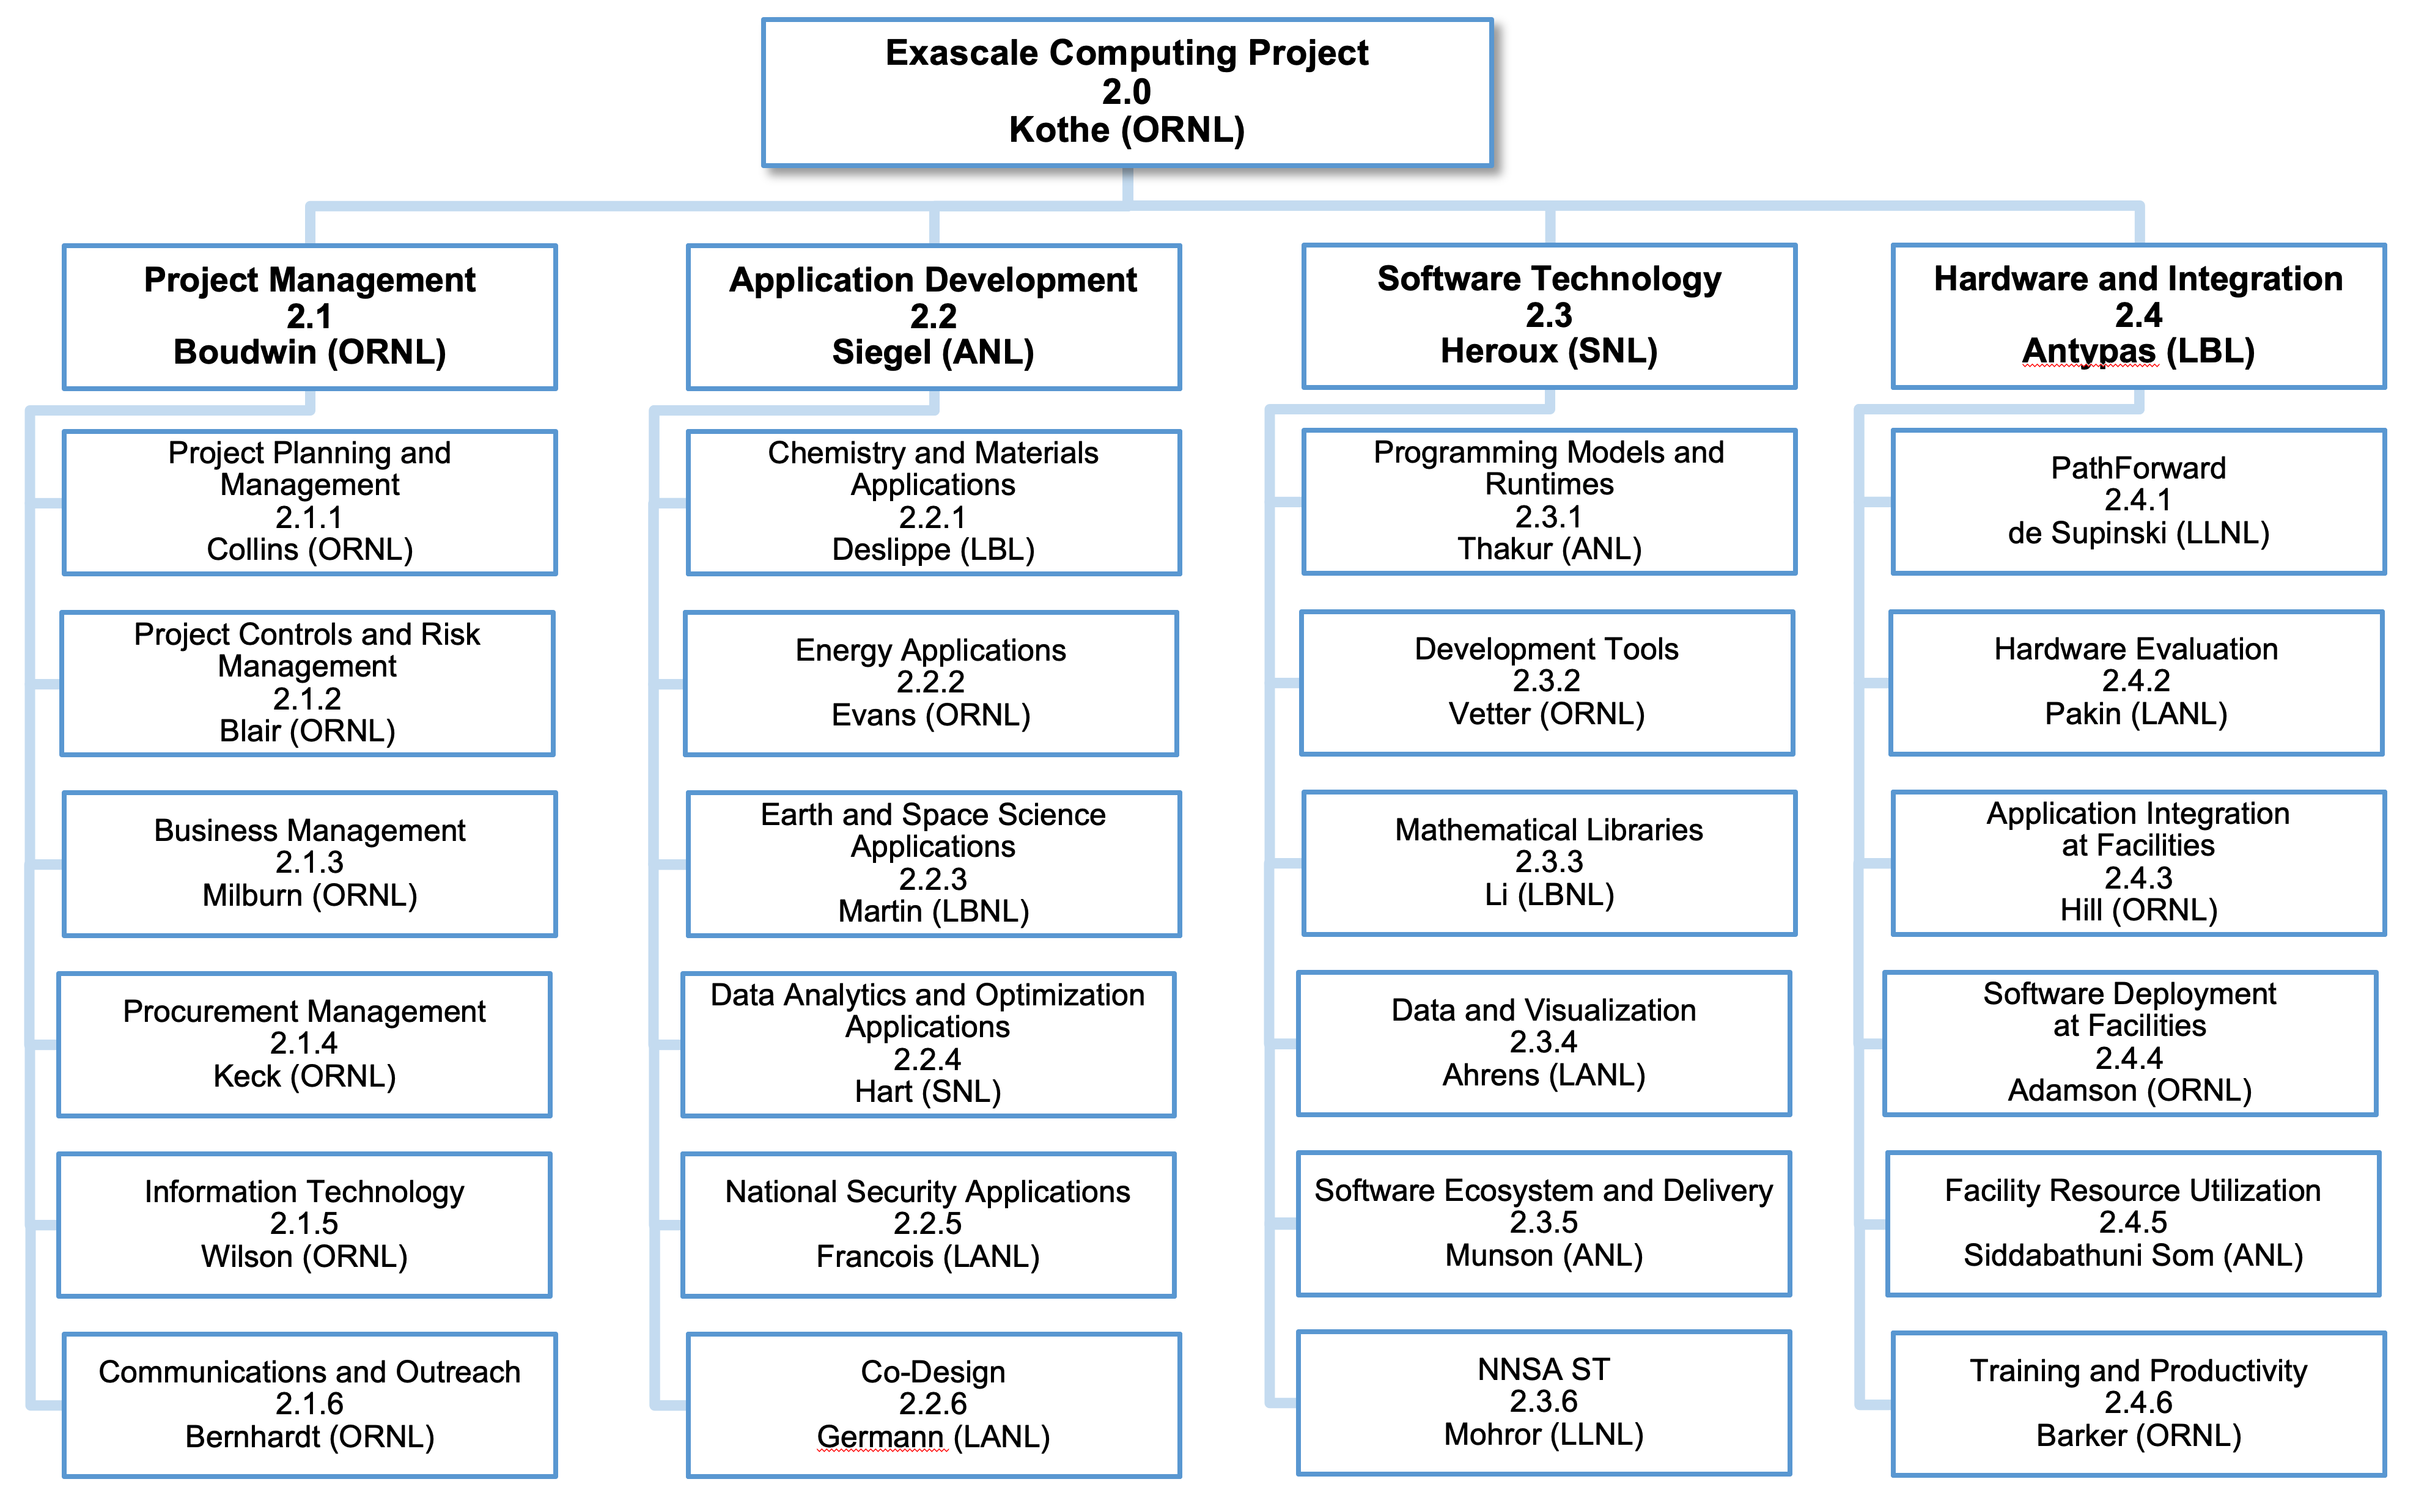
\includegraphics[width=0.9\linewidth]{ECP22}
	\caption{The ECP WBS through Level 3 (L3) as of December 5, 2019. Under ST, WBS 2.3.6 consolidates ATDM contributions to the ECP into a new L3 area.}
	\protect\todo[inline]{Please replace image with higher resolution image that is not a screenshot so that the image is not blurry and no longer has the red spellcheck underline. Also, please add a callout to Figure 1 somewhere in the text.}
	\label{fig:ecp2}
\end{figure}

\subsection{Background}
Historically, the software used on supercomputers has come from three sources: computer system vendors, DOE national laboratories, and academia. Traditionally, vendors have supplied system software, such as operating systems, compilers, runtime, and system-management software. The basic system software is typically augmented by software developed by the DOE HPC facilities to fill gaps or improve system management. System software often breaks or does not perform well when there is a jump in the scale of the system.
 
Mathematical libraries and tools for supercomputers have traditionally been developed at universities and DOE national laboratories and ported to the new computer architectures when they are deployed. Vendors also play a role in this space by optimizing the implementations of commonly used libraries and tools for their architectures while retaining the interfaces defined by the broader community.  This approach enables compile and link time replacement to improve performance on a specific platform by using the vendor versions.  Mathematical libraries and tools have been remarkably robust and have supplied some of the most impactful improvements in application performance and productivity. The challenges have been the constant adapting and tuning to rapidly changing architectures.
 
Programming paradigms and the associated programming environments---which include compilers, debuggers, message passing, and associated runtimes---have traditionally been developed by vendors, DOE laboratories, and universities. The same can be said for file system and storage software. Vendors are ultimately responsible for providing a programming environment and file system with the supercomputer, but vendors are often disinterested in software developed by others or investing in new ideas that have few or no users yet. Also, file system software plays a key role in overall system resilience, and the difficulty of making the file system software resilient has grown nonlinearly with the scale and complexity of the supercomputers.
 
In addition to the lessons learned from traditional approaches, exascale computers pose unique software challenges, including the following.
\begin{itemize}
\item \textbf{Extreme parallelism:} Experience has shown that software breaks at each shift in scale. Exascale systems are predicted to have a billion-way concurrency almost exclusively from discrete accelerator devices, similar to today's GPUs. An alternate approach that uses many cores with vector units is also competitive but still requires the same approximate amount of parallelism.  Because clock speeds have essentially stalled, the 1,000-fold increase in potential performance going from petascale to exascale is entirely from concurrency improvements.
\item \textbf{Data movement in a deep memory hierarchy: }Data movement has been identified as a key impediment to performance and power consumption. Exascale system designs are increasing the types and layers of memory, which further challenges the software to increase data locality and reuse while reducing data movement.
\item \textbf{Discrete memory and execution spaces:} The node architectures of exascale systems include host CPUs and discrete device accelerators.  Programming for these systems requires the coordinated transfer of data and work between the host and device. Although some of this transfer can be managed implicitly, for the most performance-sensitive phases, the programmer typically manages host-device coordination explicitly.  Much of the software transformation effort will focus on this issue.
\end{itemize}
 
In addition to the software challenges imposed by the scale of exascale computers, the following additional requirements push the ECP away from historical approaches of obtaining the needed software for DOE supercomputers.
\begin{itemize}
\item \textbf{2021 acceleration:} One of the ECP's goals is to accelerate the development of the US exascale systems and enable the first deployment by 2021. This means that the software must be ready soon. A concerted plan that accelerates the development of the highest priority and most impactful software is needed.
\item \textbf{Productivity:} Traditional supercomputer software requires considerable expertise to use. One of the ECP's goals is to make exascale computing accessible to a wider science community than was possible with previous supercomputers. This requires developing software that improves productivity and ease of use.
\item \textbf{Diversity:} There is a strong push to make software run across diverse exascale systems. Accelerator devices from NVIDIA have been available for many years, and specific host-device programming and execution applications have been successfully ported to these platforms.  Exascale platforms will continue to have this kind of execution model but with different programming and runtime software stacks.  Writing high-performance, portable code for these platforms will be challenging.
\item \textbf{Analytics and machine learning:} Future DOE supercomputers must solve emerging data science and machine learning problems in addition to the traditional modeling and simulation applications. This will require the development of scalable, parallel analytics and machine learning software for scientific applications, much of which does not exist today.
\end{itemize}
 
\noindent The next section describes the approach the ECP ST used to address the exascale challenges.

\subsection{ECP ST Project WBS changes}\label{subsect:ProjectRestructuring}

The initial organization of the ECP ST was based on discussions that occurred over several years of exascale planning within DOE, especially DOE ASCR.  Figure~\ref{fig:ecpstv1} \todo{Should this be Figure 1? The first 3 figures in this document are not called out. Recommend calling them out prior to this or moving them behind fig:ecpstv1.} shows the conceptual diagram of this first phase.  The 66 ECP ST projects were mapped into eight technical areas, in some cases arbitrating where a project should go based on its primary type of work, even if other work were present in the project.  In November 2017, the ECP ST was reorganized into five technical areas, primarily through merging a few smaller areas, and the number of projects was reduced to 56, then to 55 because of further merging in \ecosystem.  Figure~\ref{fig:ecpstv2} shows the diagram of the second phase of the ECP ST.  Section~\ref{sect:PETA} describes the organization, planning, execution, tracking, and assessment processes that will put the ECP ST in a good position for success in the critical decision (CD) 2 phase of the project.

\begin{figure}
	\centering
	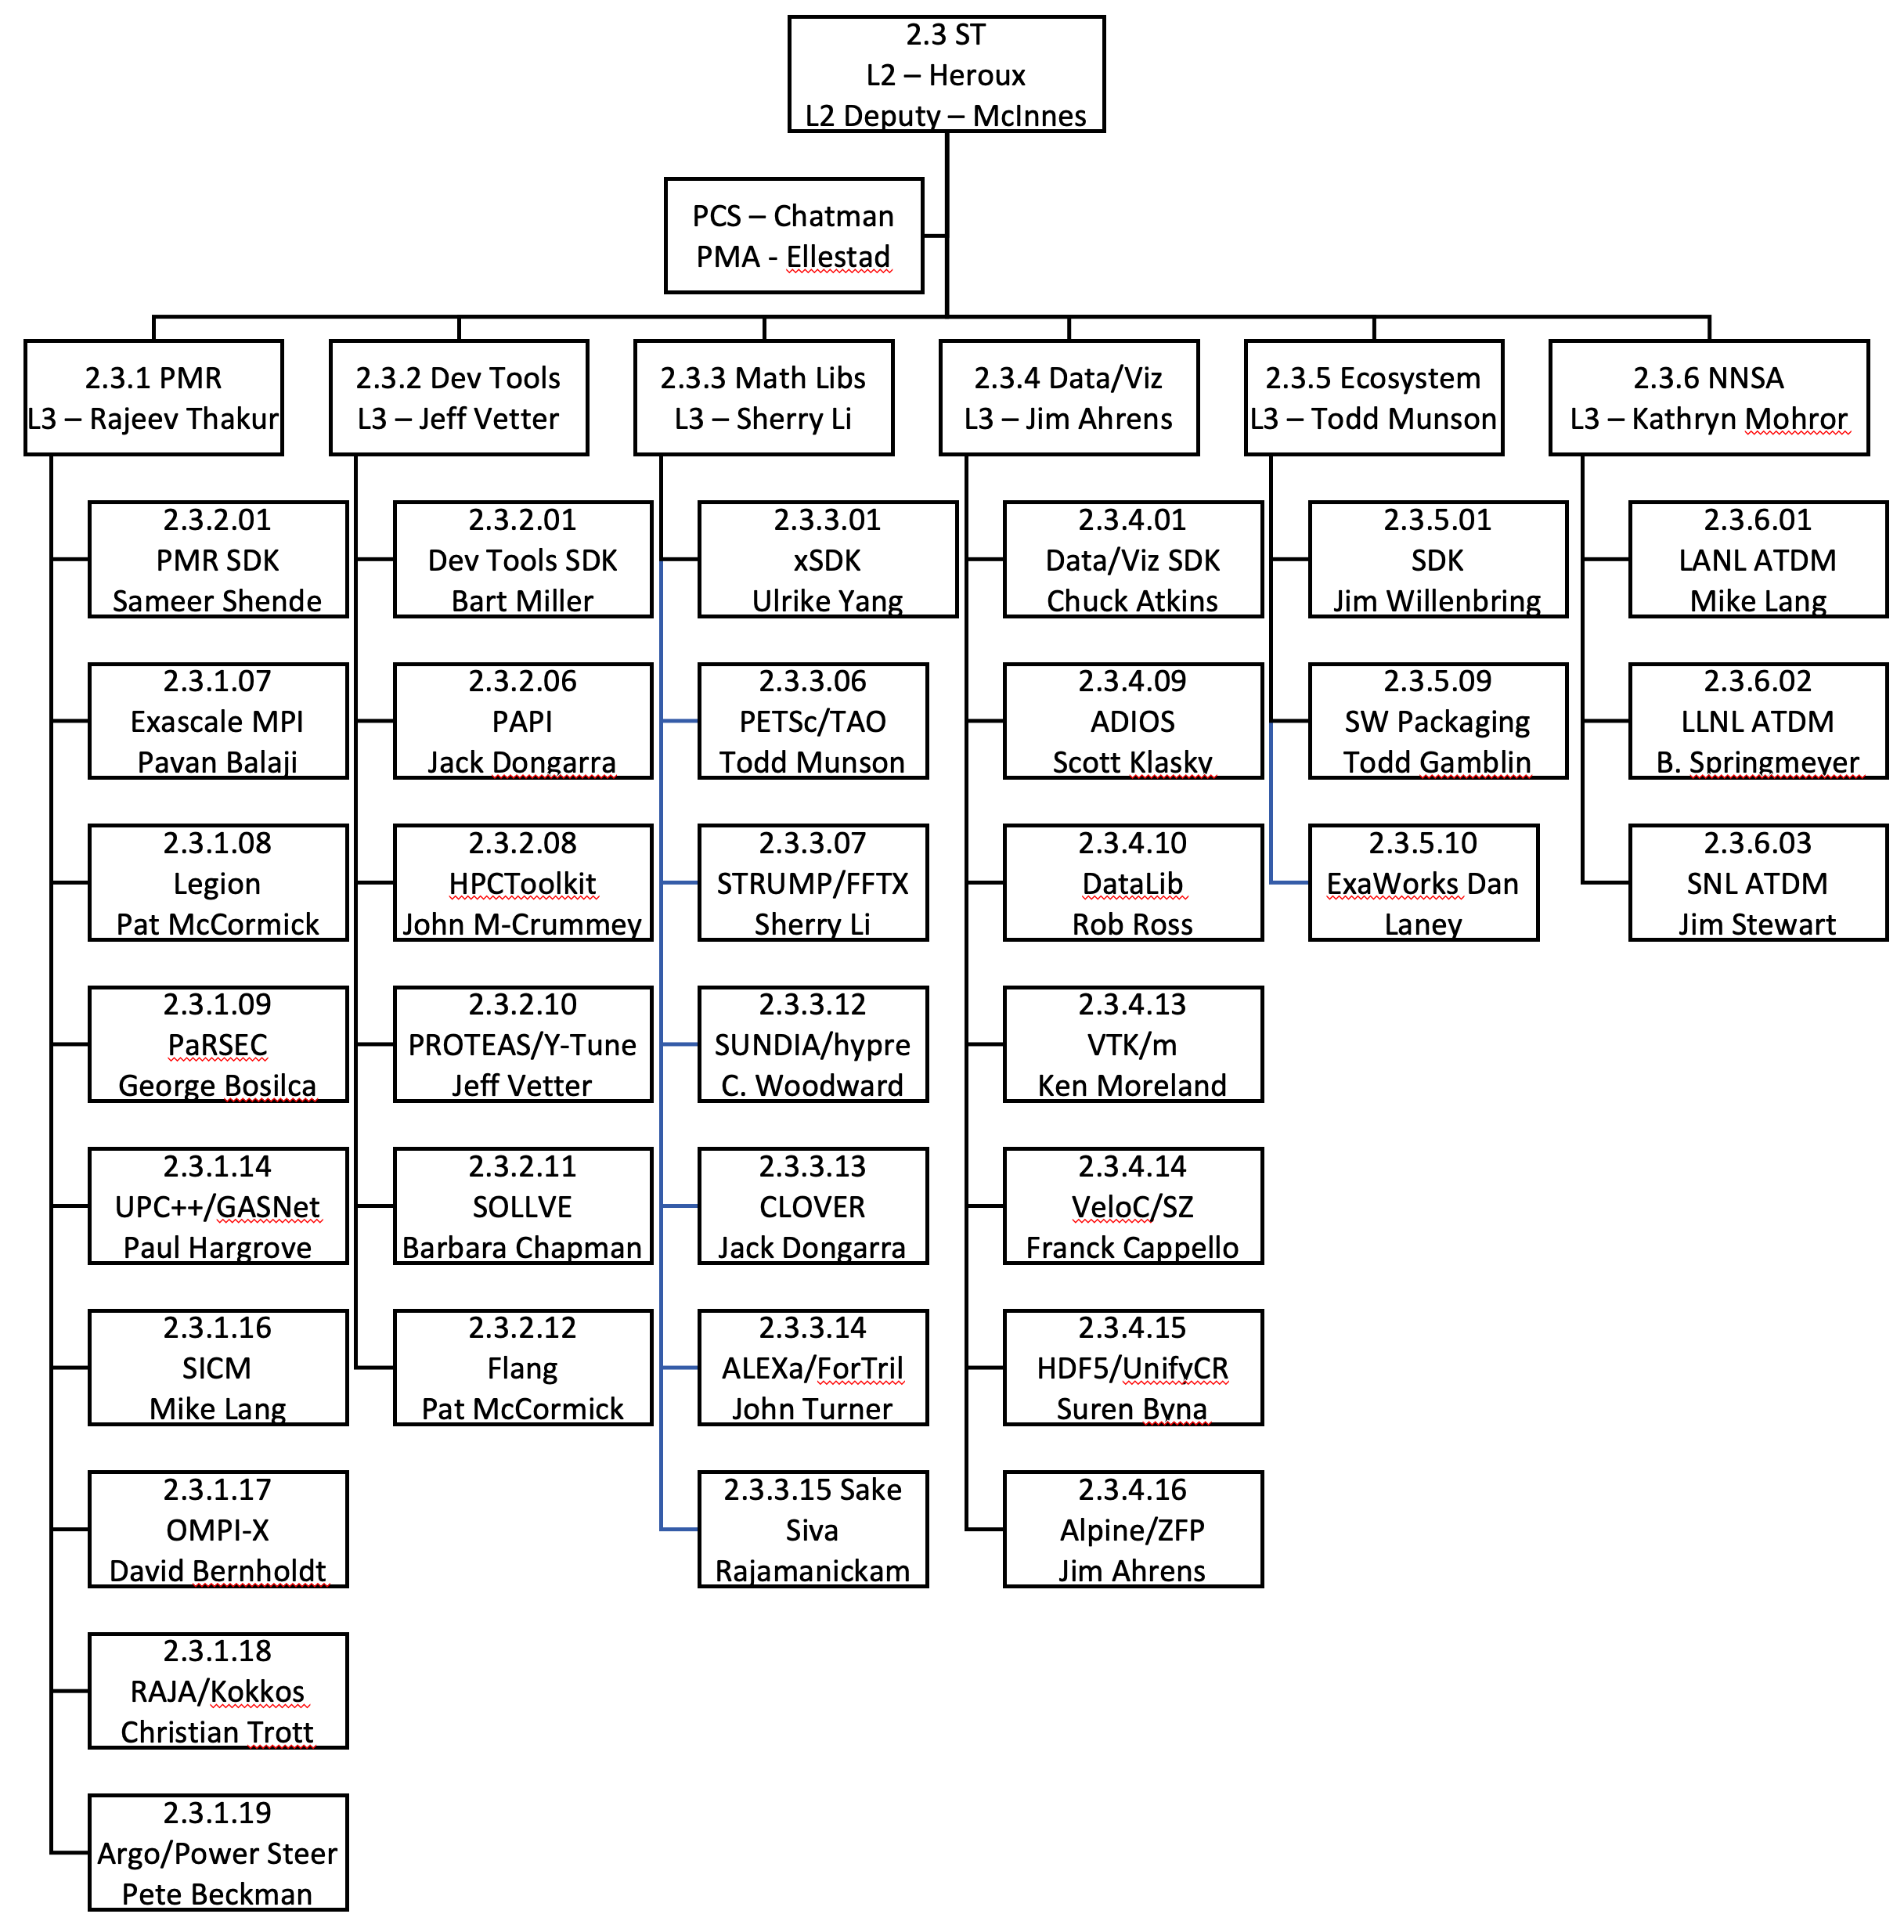
\includegraphics[width=0.9\linewidth]{STFY20WBS}
	\caption{\label{fig:wbs-FY20} The FY20 ECP ST WBS as of November 18, 2020, includes two new Level 4 (L4) subprojects: 2.3.5.10 ExaWorks, a workflow components project, and 2.3.3.15 Sake, a new solver effort that provides funding for Trilinos porting to Frontier and Aurora platforms.}
    \protect\todo[inline]{Please replace image with higher resolution image that is not a screenshot so that the image is not blurry and no longer has the red spellcheck underline.}
\end{figure}

\begin{figure}
\begin{mdframed}
\todo[inline]{Would this be better suited as a list with a header in the narrative?}
\begin{itemize}
\item Phase 1: 66 total L4 subprojects
\begin{itemize}
\item 35 projects funded by DOE SC that were selected in late 2016 via an RFI and RFP process, considering prioritized requirements of applications and DOE facilities. 
These projects started work between January--March 2017, depending on when the contracts were awarded.
\item 31 ongoing DOE NNSA-funded projects that are part of the ATDM program. The ATDM program started in FY14.  These projects are focused on longer term research to address the shift in computing technology to extreme heterogeneous architectures and to advance the capabilities of NNSA simulation codes.
\end{itemize}
\item Phase 2: 55 total L4 subprojects
\begin{itemize}
\item 41 ASCR-funded projects.  Added  two \ecosystem\ projects and four SDK projects.
\item 15 ATDM projects: Combined the previous 31 ATDM projects into one project per technical area per lab.  ATDM projects are generally more vertically integrated and would not perfectly map to any proposed ECP ST technical structure.  Minimizing the number of ATDM projects within the ECP WBS reduces complexity of ATDM to ECP coordination and gives ATDM flexibility in revising its portfolio without disruption to the ECP-ATDM mapping.
\end{itemize}
\item Phase 3a: 33 total L4 subprojects.  Fewer, larger, and more uniform-sized projects.
\begin{itemize}
	\item Starting in FY20, the ECP ST further consolidated L4 projects to foster additional synergies and amortize project overheads as the ECP heads into the CD-2 phase~\cite{413.3B}, in which more rigorous planning and execution are needed.
	\item Five L3s to six: New NNSA ST L3.
	\item 40 ST SC-funded L4 subprojects to 30.
	\begin{itemize}
	\item \pmr: 13 to nine, \tools: six to six, \mathlibs: seven to six, \dataviz: 10 to seven, \ecosystem: four to three.
	\item Includes two new L4 subprojects in \ecosystem.
	\end{itemize}
	\item 15 ST NNSA-funded projects transferred to new NNSA ST L3. Consolidated from 15 to three L4 subprojects.
	\item No more small subprojects.
	\item Figure~\ref{fig:wbs-FY20} shows the overall structure.\todo[inline]{First callout to Figure 2 is within Figure 3. Please correct.}
\end{itemize}
\item Phase 3b: 35 total L4 subprojects.  Add two new L4 subprojects.
\begin{itemize}
	\item New L4 subproject called ExaWorks.  Focuses on providing an underlying component architecture for workflow management systems and is led by a team of workflow experts who would leverage the new substrate in their own workflow products.
	\item New L4 subproject called Sake.  This project was created in response to a need for Trilinos funding to port to Aurora and Frontier.  Concurrently, Trilinos-related activities in the CLOVER project, specifically Kokkos Kernels, were merged with the new Trilinos funding to create a more holistic project independent of CLOVER.
	\item Figure~\ref{fig:wbs-FY20} shows the overall structure.
\end{itemize}
\end{itemize}
\end{mdframed}

\caption{\label{fig:project-remapping}Project remapping summary from Phase 1 (through November 2017) to Phase 2 (November 2017--September 30, 2019) to Phase 3 (After October 1, 2019).}
\end{figure}


\begin{figure}
	\centering
	\includegraphics[width=0.9\linewidth]{ECPSTV1}
	\caption{The ECP ST before the November 2017 reorganization.  This conceptual layout emerged from several years of exascale planning conducted primarily within DOE ASCR.  Because of significant restructuring of the ECP that removed many of the facility's activities and reduced the project time line from 10 to 7 years, as well as a growing awareness of what risks had diminished, this diagram no longer represented the ECP ST efforts accurately.}
	\label{fig:ecpstv1}
	\todo[inline]{Please add a ref to this figure in the narrative.}
\end{figure}
\begin{figure}
	\centering
	\includegraphics[width=0.9\linewidth]{ECPSTV2}
	\caption{The ECP ST after the November 2017 reorganization.  This diagram more accurately reflects the priorities and efforts of the ECP ST given the new ECP project scope and the demands foreseen.}
	\label{fig:ecpstv2}
	\todo[inline]{Please add a ref to this figure in the narrative.}
\end{figure}
\begin{figure}
	\centering
	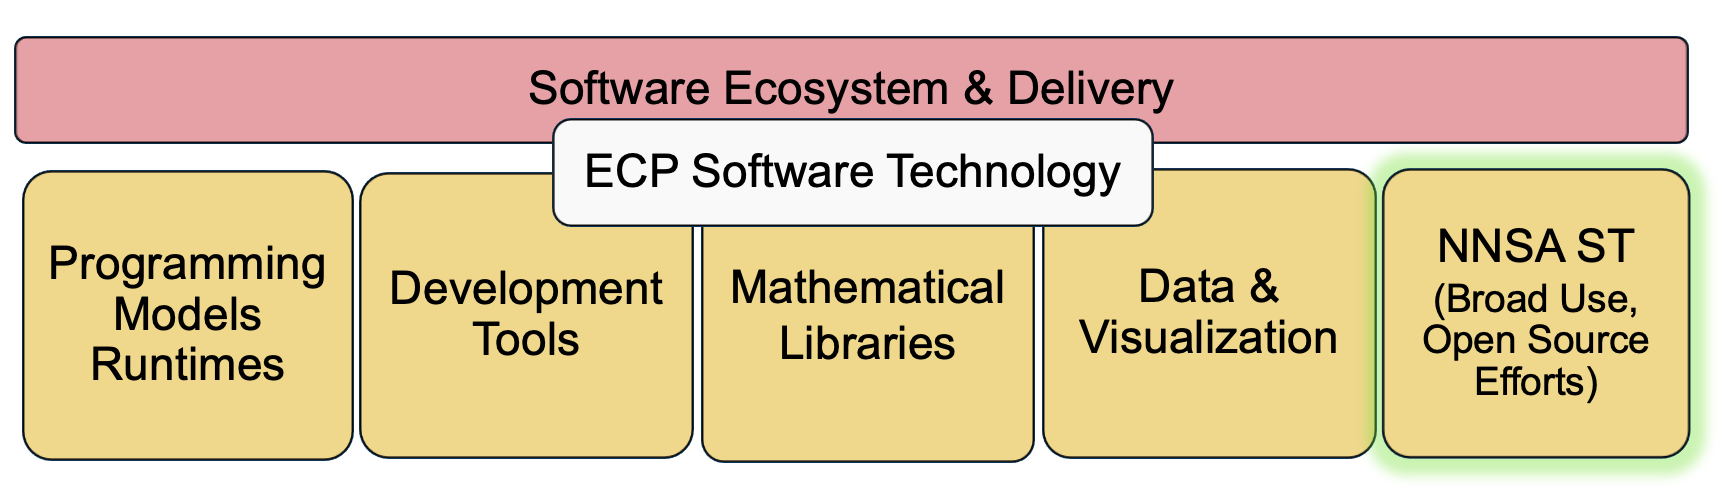
\includegraphics[width=0.9\linewidth]{ECPSTV3}
	\caption{The ECP ST after the October 2019 reorganization.  This diagram reflects the further consolidation of NNSA open-source contributions to enable the more flexible management of NNSA ST contributions.}
	\todo[inline]{Please add a ref to this figure in the narrative.}
\end{figure}
\begin{figure}
	\centering
	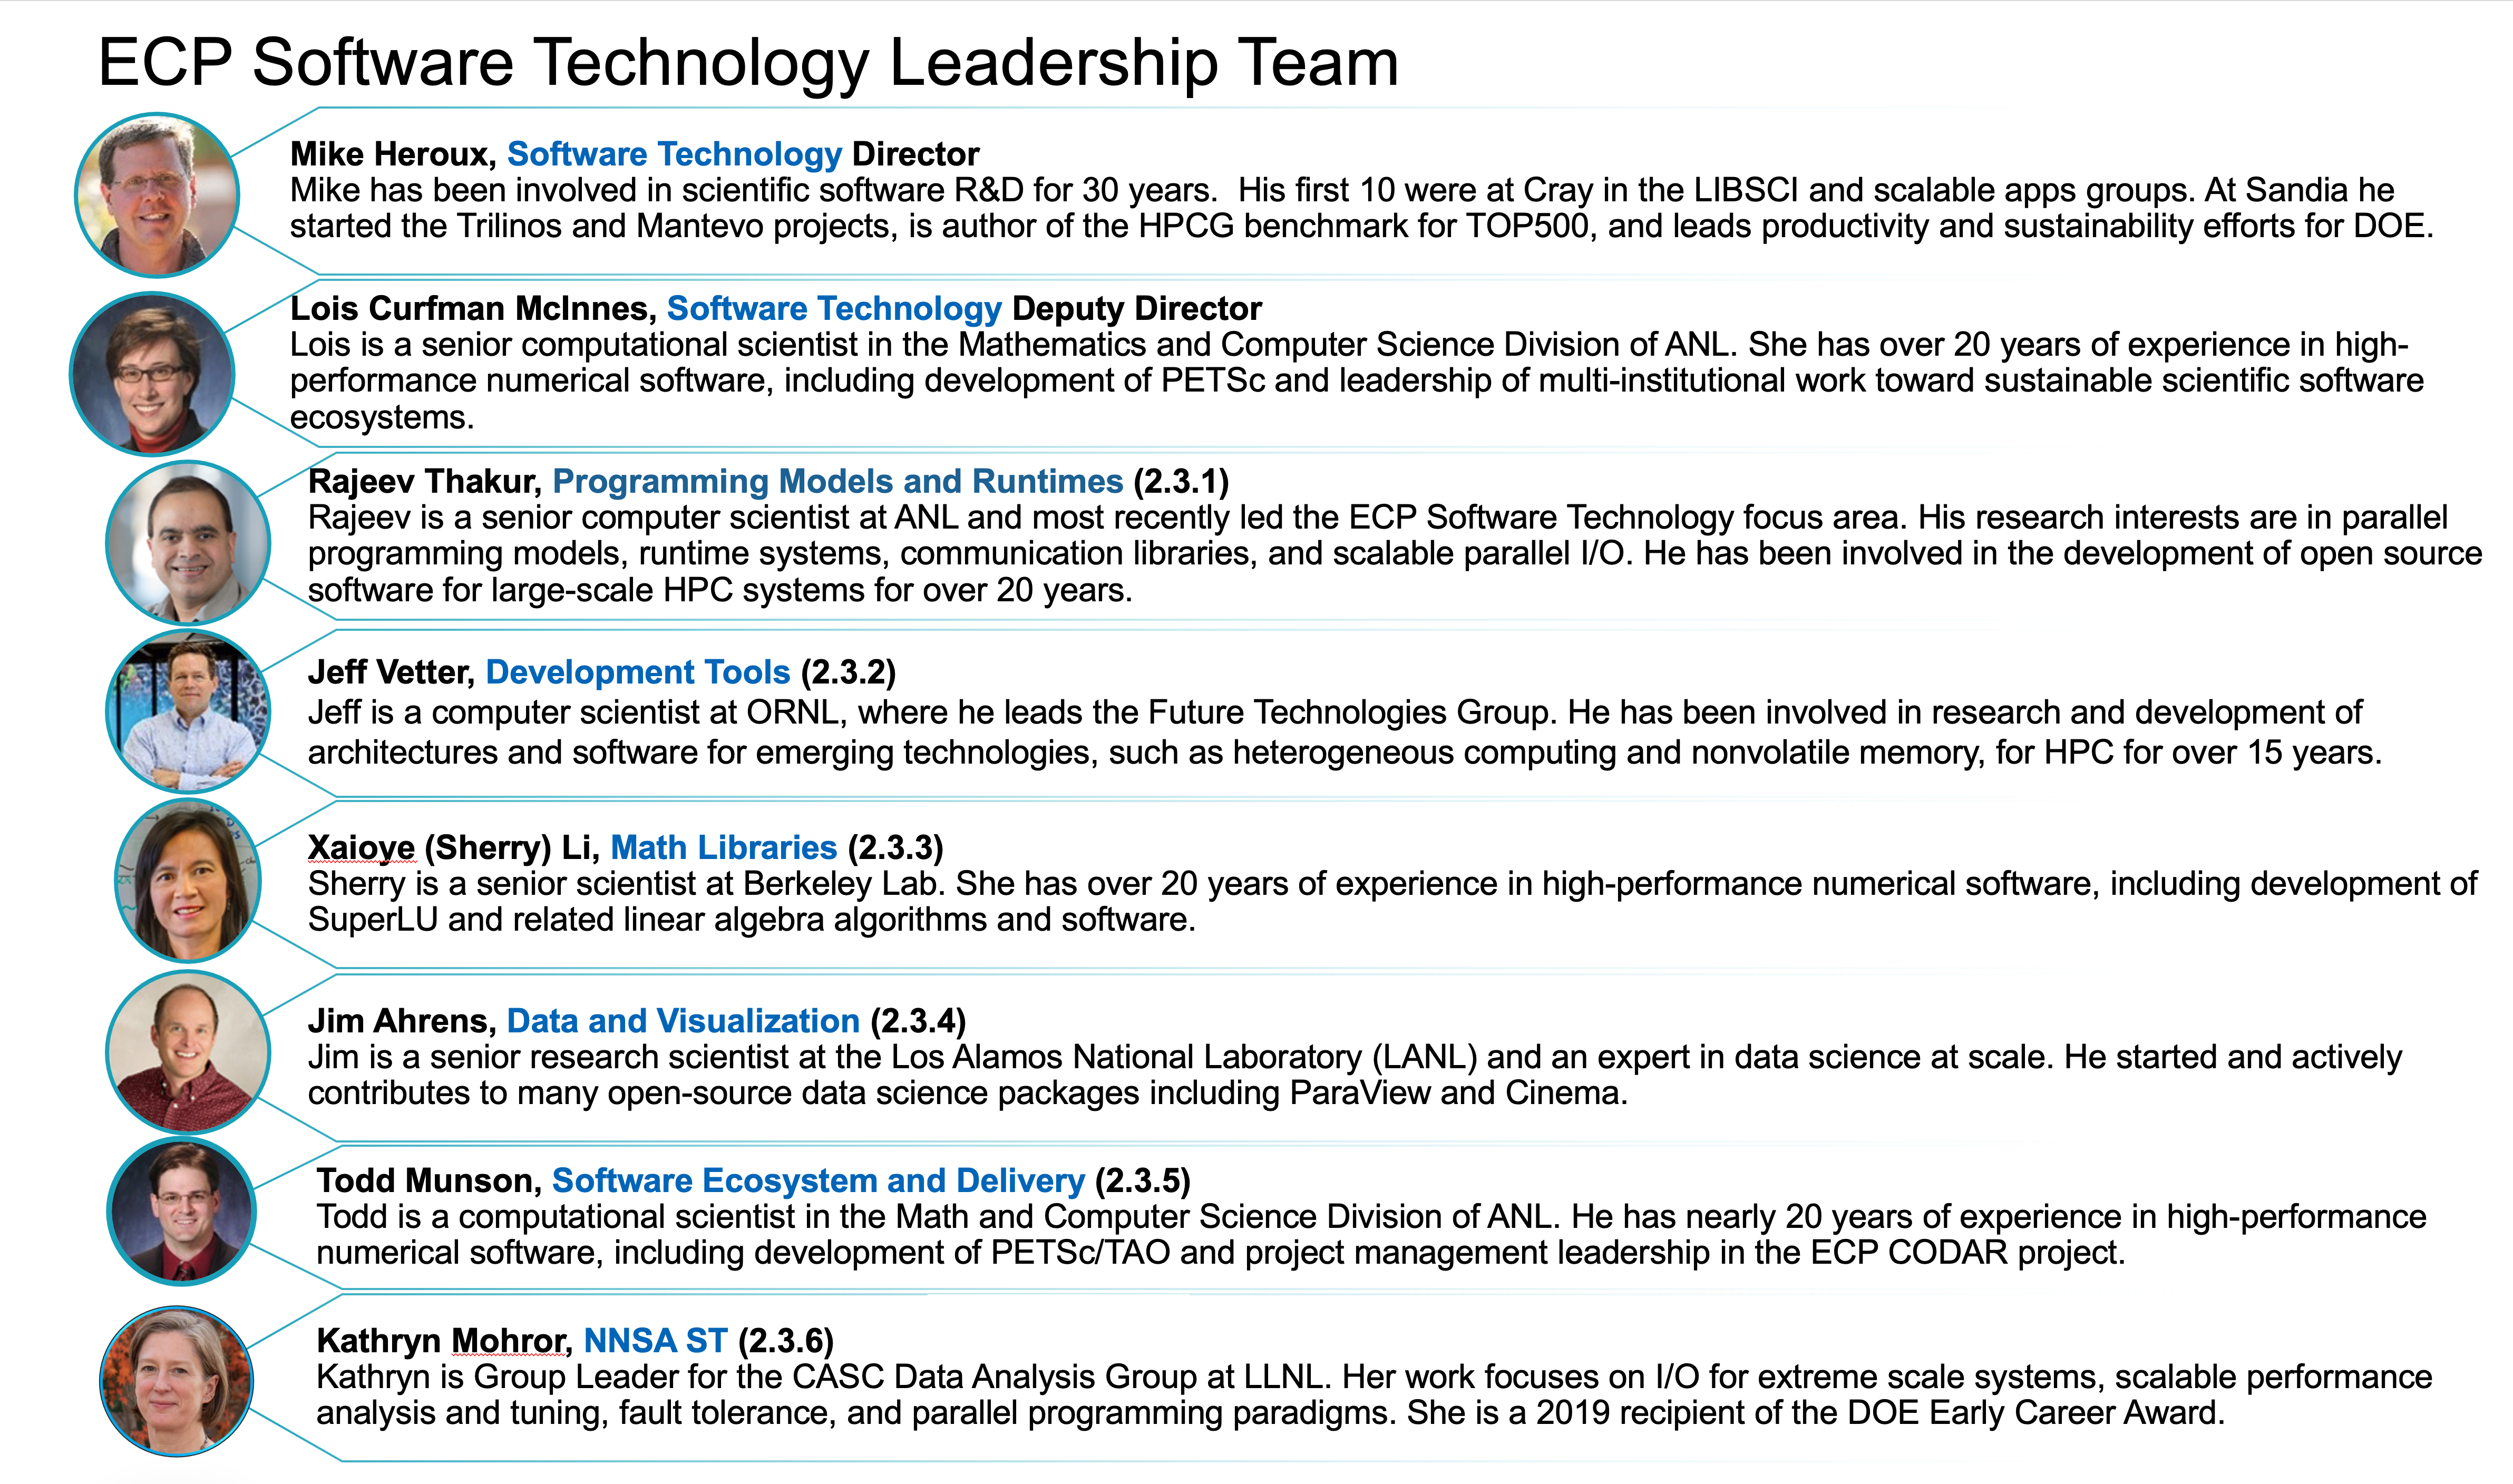
\includegraphics[width=0.9\linewidth]{ECP-ST-Leads}
	\caption{The ECP ST Leadership Team as of November 2020. Jonathan Carter, previous deputy director of the ECP ST, became associate laboratory director of the Computing Sciences Area at Lawrence Berkeley National Laboratory. His departure led to Lois Curfman McInnes, previously the L3 lead of Mathematical Libraries, being named the ECP ST deputy director and Sherry Li being named the new Mathematical Libraries L3 lead.  Rob Neely was also promoted at Lawrence Livermore National Laboratory (LLNL), leading to Kathryn Mohror becoming the L3 lead of NNSA ST.}
	\label{fig:ecpstleads}
	\todo[inline]{Please add a ref to this figure in the narrative.}
\end{figure}



\section{ECP ST Planning, Execution, Tracking and Assessment}\label{sect:PETA}
During the last 2 years, the ECP ST has introduced the E4S and SDKs.  New approaches have been established for project planning, execution, tracking, and assessment by using a tailored earned value management system that enables iterative and incremental refinement to its planning process.  The team has also revised its key performance parameter (KPP) to be solely focused on measuring capability integration into client environments.  An assessment process was developed and used that has led to significant changes in the number and scope of L4 subprojects.

\subsection{ECP ST Architecture and Design}
The ECP is taking an approach of co-design across all its principal technical areas: Application Development (AD), ST, and Hardware and Integration (HI). For the ECP ST, this means that its requirements are based on input from other areas, and there is a tight integration of the software products within the software stack and with applications and the evolving hardware. 

The ECP ST portfolio of projects is intended to address the aforementioned exascale challenges and requirements. The ECP is not developing the entire software stack for an exascale system. For example, vendors are expected to provide the core software that comes with the system---in many cases, by leveraging ECP and other open-source efforts. Examples of vendor-provided software include operating systems; file systems; compilers for C, C++, Fortran, and so on, increasingly derived from the LLVM community ecosystem to which the ECP contributes; basic math libraries; system monitoring tools; schedulers; debuggers; vendor performance tools; MPI based on ECP-funded projects; OpenMP with features from ECP-funded projects; and data-centric stack components. The ECP develops other, mostly higher level software that is needed by applications and is not vendor specific. ECP-funded software activities are concerned with extreme scalability, exposing additional parallelism, unique requirements of exascale hardware, and performance-critical components. Other software that aids in developer productivity is needed and could come from third-party, open-source efforts.

The ST portfolio includes both ASCR and NNSA ATDM-funded efforts. The memorandum of understanding established between DOE SC and NNSA has formalized this effort.  Whenever possible, ASCR and ATDM efforts are treated uniformly in ECP ST planning and assessment activities.

ST also plans to increase integration within the ST portfolio through the increased use of software components and application composition vs. monolithic application design. One important transition that ECP can accelerate is the increased development and delivery of reusable scientific software components and libraries. Although math and scientific libraries have long been a successful element of the scientific software community, their use can be expanded to include other algorithms and software capabilities so that applications can be considered more of an aggregate composition of reusable components than a monolithic code that uses libraries tangentially.

To accelerate this transition, a greater commitment on the part of software component developers is needed to provide reliable and portable software that users can consider to be part of the software ecosystem in much the same way users depend on MPI and compilers. However, application developers must be expected to participate as clients and users of reusable components, using capabilities from components, transitioning away from---or keeping a backup option of---their own custom capabilities.

\subsubsection{The Extreme-Scale Scientific Software Stack}\label{subsubsect:e4s}
In October 2020, the ECP ST released V1.2 of the E4S.\footnote{\url{http://e4s.io}} E4S contains a collection of the software products to which ECP ST contributes.  E4S is the primary conduit for providing easy access to ECP ST capabilities for the ECP and the broader community.  E4S is also the ECP ST vehicle for regression and integration testing across DOE pre-exascale and exascale systems.

\begin{figure}
		\centering
		\fbox{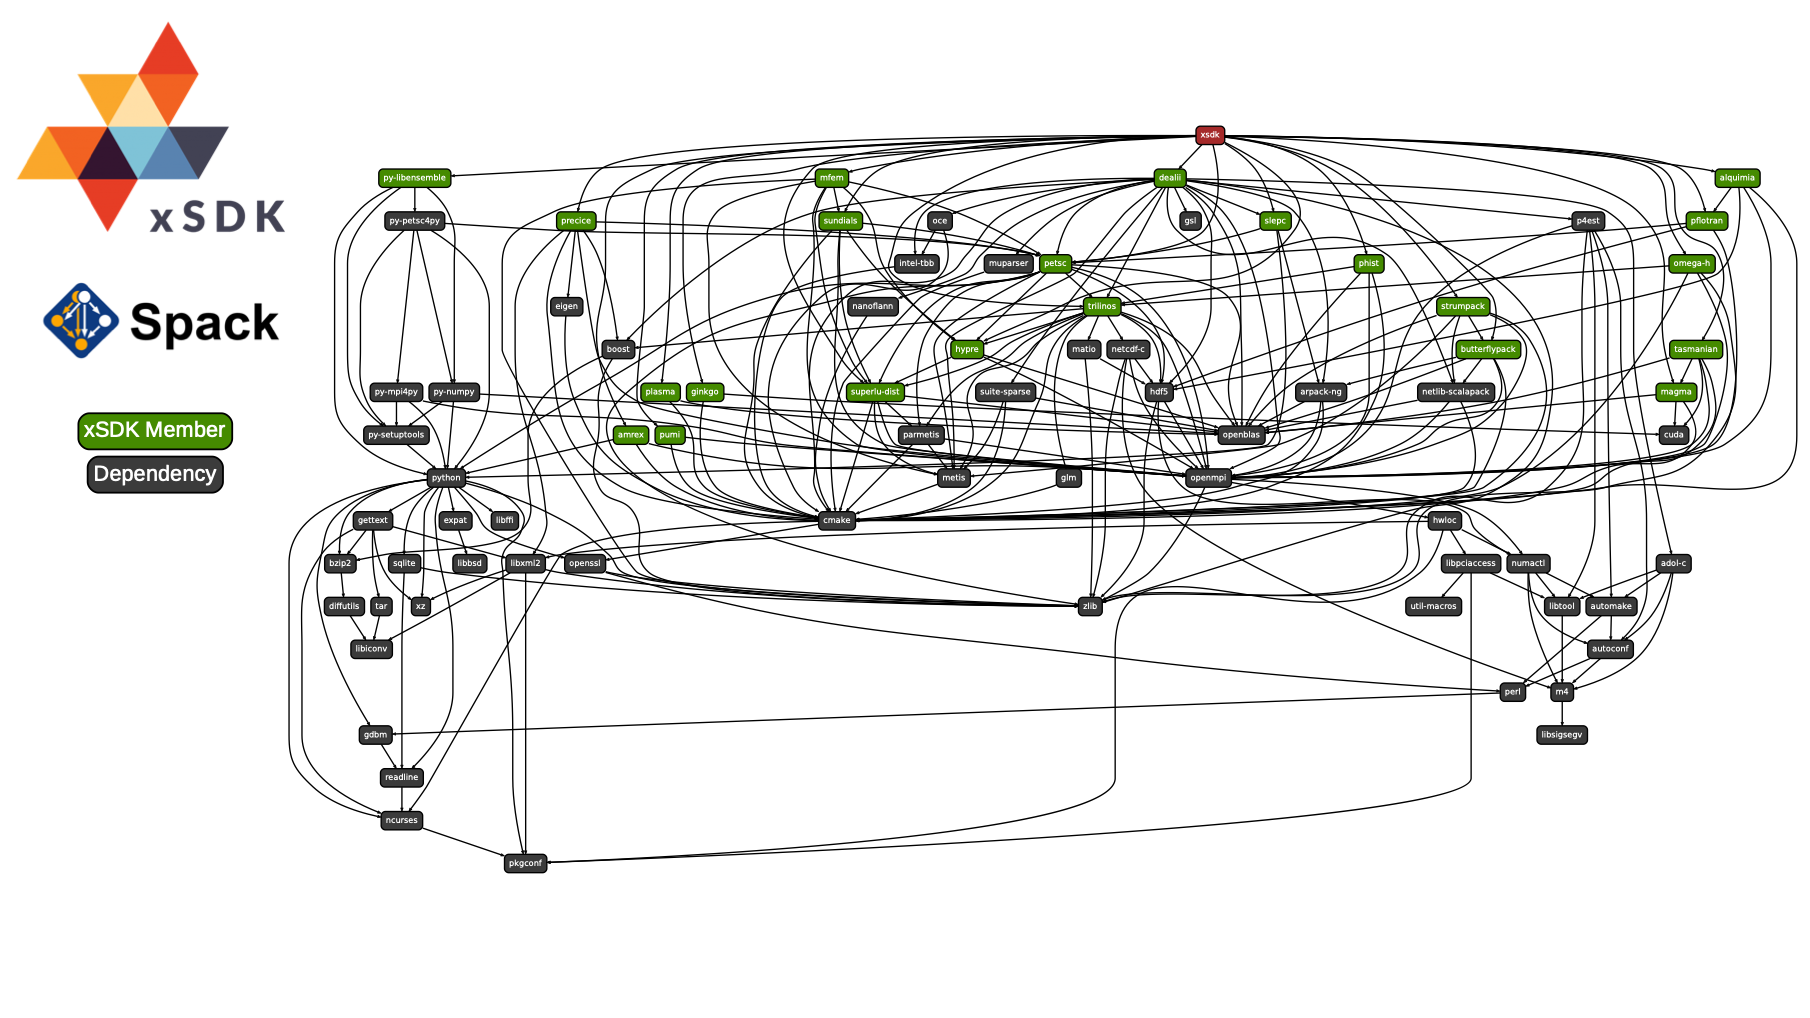
\includegraphics[width=0.9\linewidth]{E4S-Build-Tree}}
	\caption{Using Spack~\cite{gamblin+:ecp18-spack-tutorial}, E4S builds a comprehensive software stack.  As ECP ST efforts proceed, E4S will be used for continuous integration testing, providing developers with rapid feedback on regression errors and providing user facilities with a stable software base as the team prepares for exascale platforms.  This diagram shows how E4S builds ECP products via an SDK target, which are the math libraries' SDK, called xSDK in this example.  The SDK target then builds all products that are part of the SDK (see Figure~\ref{fig:sdk-definition1-0} for SDK groupings), first defining and building external software products. Green-labeled products are part of the SDK. The blue label indicates expected system tools, which, in this case, is a particular version of Python.  Black-labeled products are expected to be previously installed into the environment, which is a common and easily satisfied requirement.  Using this approach, users interested in only SUNDIALS, a particular math library, can be assured that the SUNDIALS build will be possible because it is a portion of what E4S builds and tests.}
	\label{fig:e4s-build-tree}
\end{figure}

E4S has the following key features.
\begin{itemize}
	\item \textbf{The E4S suite is a large and growing effort to build and test a comprehensive scientific software ecosystem.} In November 2018, E4S V0.1 contained 25 ECP products.  Two years later, E4S V1.2, the fifth E4S release, contained 67 ECP ST products and numerous additional products needed for a complete software environment.  Eventually, E4S will contain all the open-source products to which ECP contributes and all the related products needed for a holistic environment.
	\item \textbf{E4S is not an ECP-specific software suite.}  The products in E4S represent a holistic collection of capabilities that contain the ever-growing SDK collections sponsored by the ECP and all additional underlying software required to use ECP ST capabilities.  Furthermore, the E4S effort is expected to live beyond the time span of the ECP, becoming a critical element of the scientific software ecosystem.
	\item \textbf{E4S is partitionable.} E4S products are built and tested together by using a tree-based hierarchical build process.  Because the entire E4S tree is built and tested, users can build any subtree of interest without building the whole stack (Figure~\ref{fig:e4s-build-tree}).
	\item \textbf{E4S uses Spack.} The Spack~\cite{gamblin+:ecp18-spack-tutorial} meta-build tool invokes the native build process of each product, enabling the quick integration of new products, including non-ECP products.
	\item \textbf{E4S is available via containers.} In addition to a build-from-source capability using Spack, E4S maintains several container environments (e.g., Docker, Singularity, Shifter, CharlieCloud) that provide the lowest barrier to use.  Container distributions dramatically reduce installation costs and provide a ready-made environment for tutorials that leverage E4S capabilities.  For example, E4S containers now support custom images for ECP applications, such as WDMapp and Pantheon.
	\item \textbf{E4S distribution.} E4S products are available at the E4S website.\footnote{\url{http://e4s.io}}
	\item \textbf{E4S developer community resources.} Developers interested in participating in E4S can visit the E4S-Project GitHub community.\footnote{\url{https://github.com/E4S-Project}}	
\end{itemize}

The first set of E4S community policies~\cite{e4s:policies} was adopted in October 2020 (Figure~\ref{fig:E4S-Community-Policies-V1}). These policies are membership criteria for a product to become an E4S member package. The purpose of the community policies is to establish baseline software quality and practice expectations to help address sustainability and interoperability challenges for the ST software ecosystem. Although a package does not have to demonstrate compatibility with the policies as a condition of inclusion in E4S releases, compatibility is necessary for member package designation.

\begin{figure}
        \centering
        \fbox{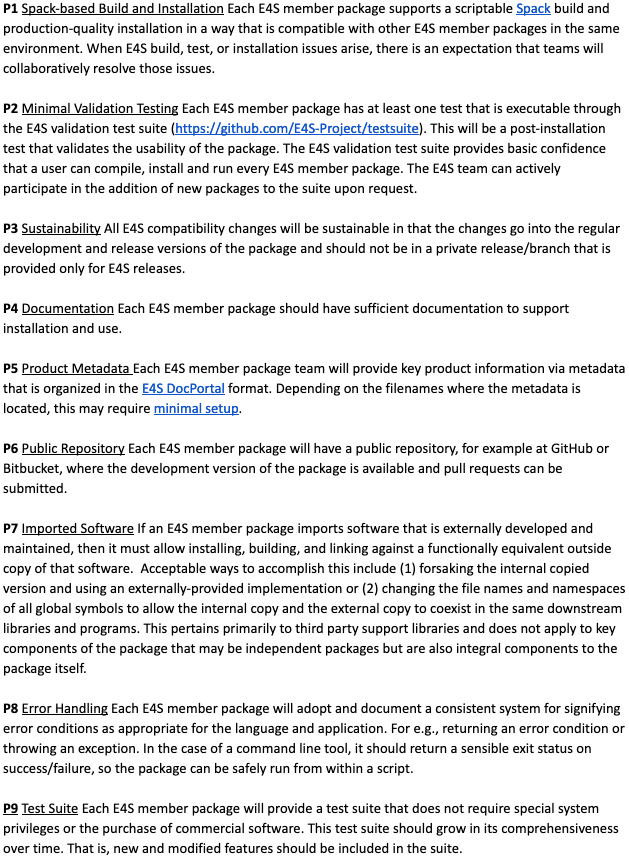
\includegraphics[width=0.9\linewidth]{E4S-Community-Policies-V1}}
        \caption{Version 1 of the E4S community policies. These policies serve as membership criteria for E4S member packages. The E4S community policy effort heavily leveraged the existing xSDK community policies~\cite{xsdk-policies:homepage}.}
          \protect\todo[inline]{Please replace image with higher resolution image so that the image is not blurry or integrate as an editable list.}
        \label{fig:E4S-Community-Policies-V1}
\end{figure}

\begin{figure}
	\centering
	\fbox{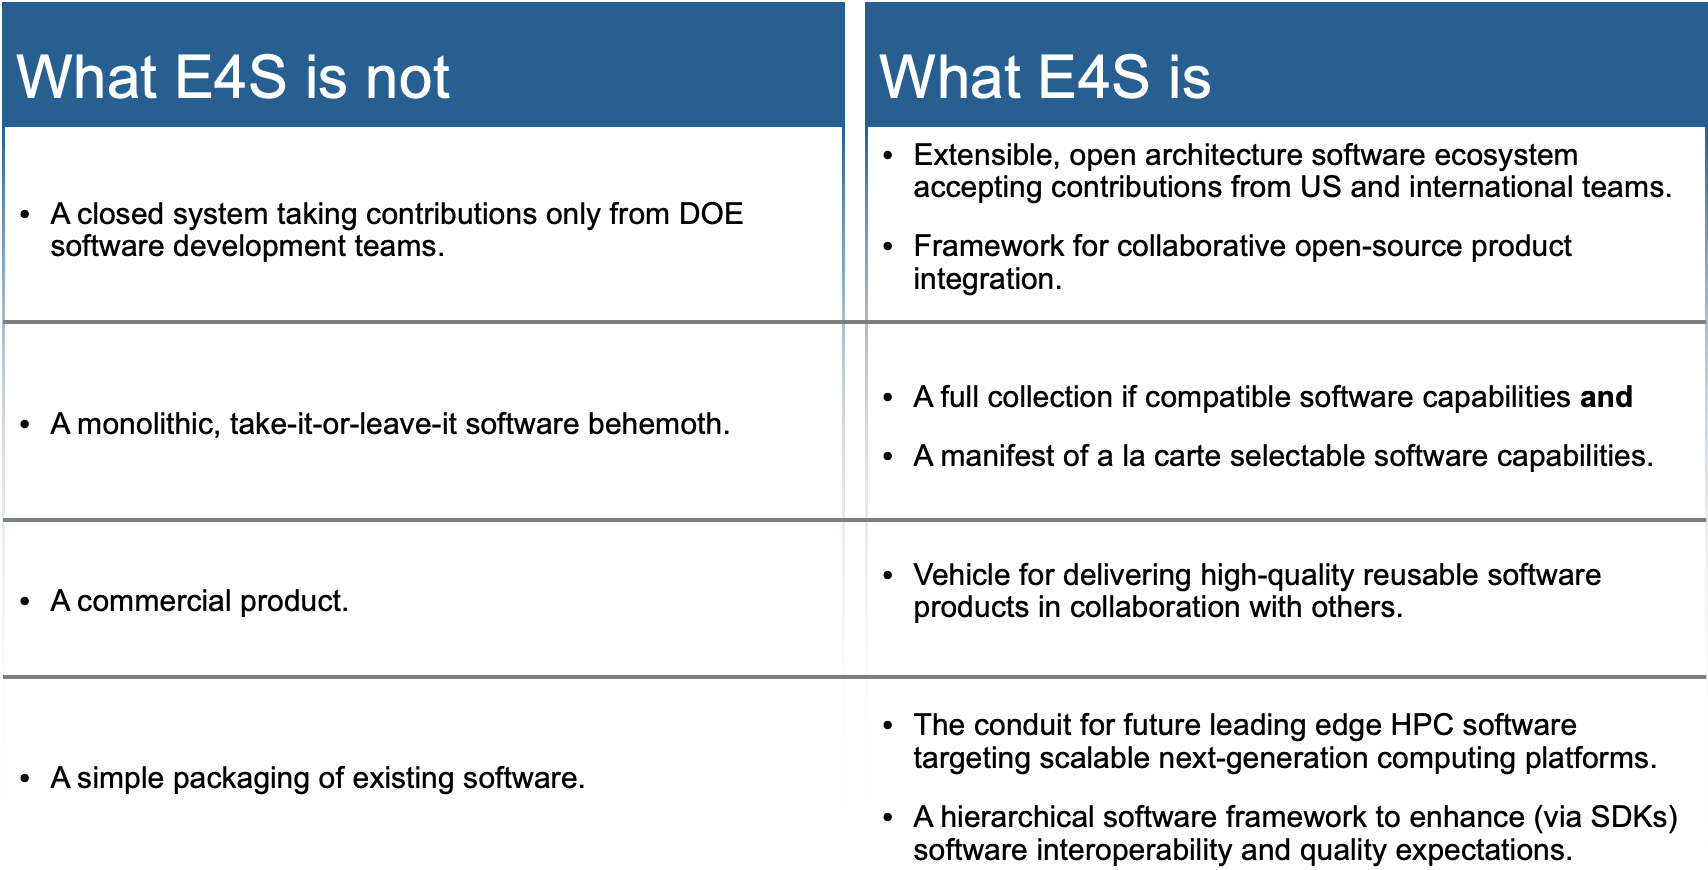
\includegraphics[width=0.9\linewidth]{E4S-Summary}}
	\caption{E4S provides a complete Linux-based software stack that is suitable for many scientific workloads, tutorial, and development environments.  Additionally, it is an open-software architecture that can expand to include any additional and compatible Spack-enabled software capabilities. Because Spack packages are available for many products and easily created for others, E4S is practically expandable to include almost any robust Linux-based product.  Furthermore, E4S capabilities are available as subtrees of the full build. E4S is not monolithic.}
    \protect\todo[inline]{Please make this a table, not a figure, so that it can be edited.}
    \todo[inline]{Please add a ref to this figure (or as a table) in the narrative.}
	\label{fig:e4s-is-isnot}
\end{figure}

\begin{figure}
	\centering
	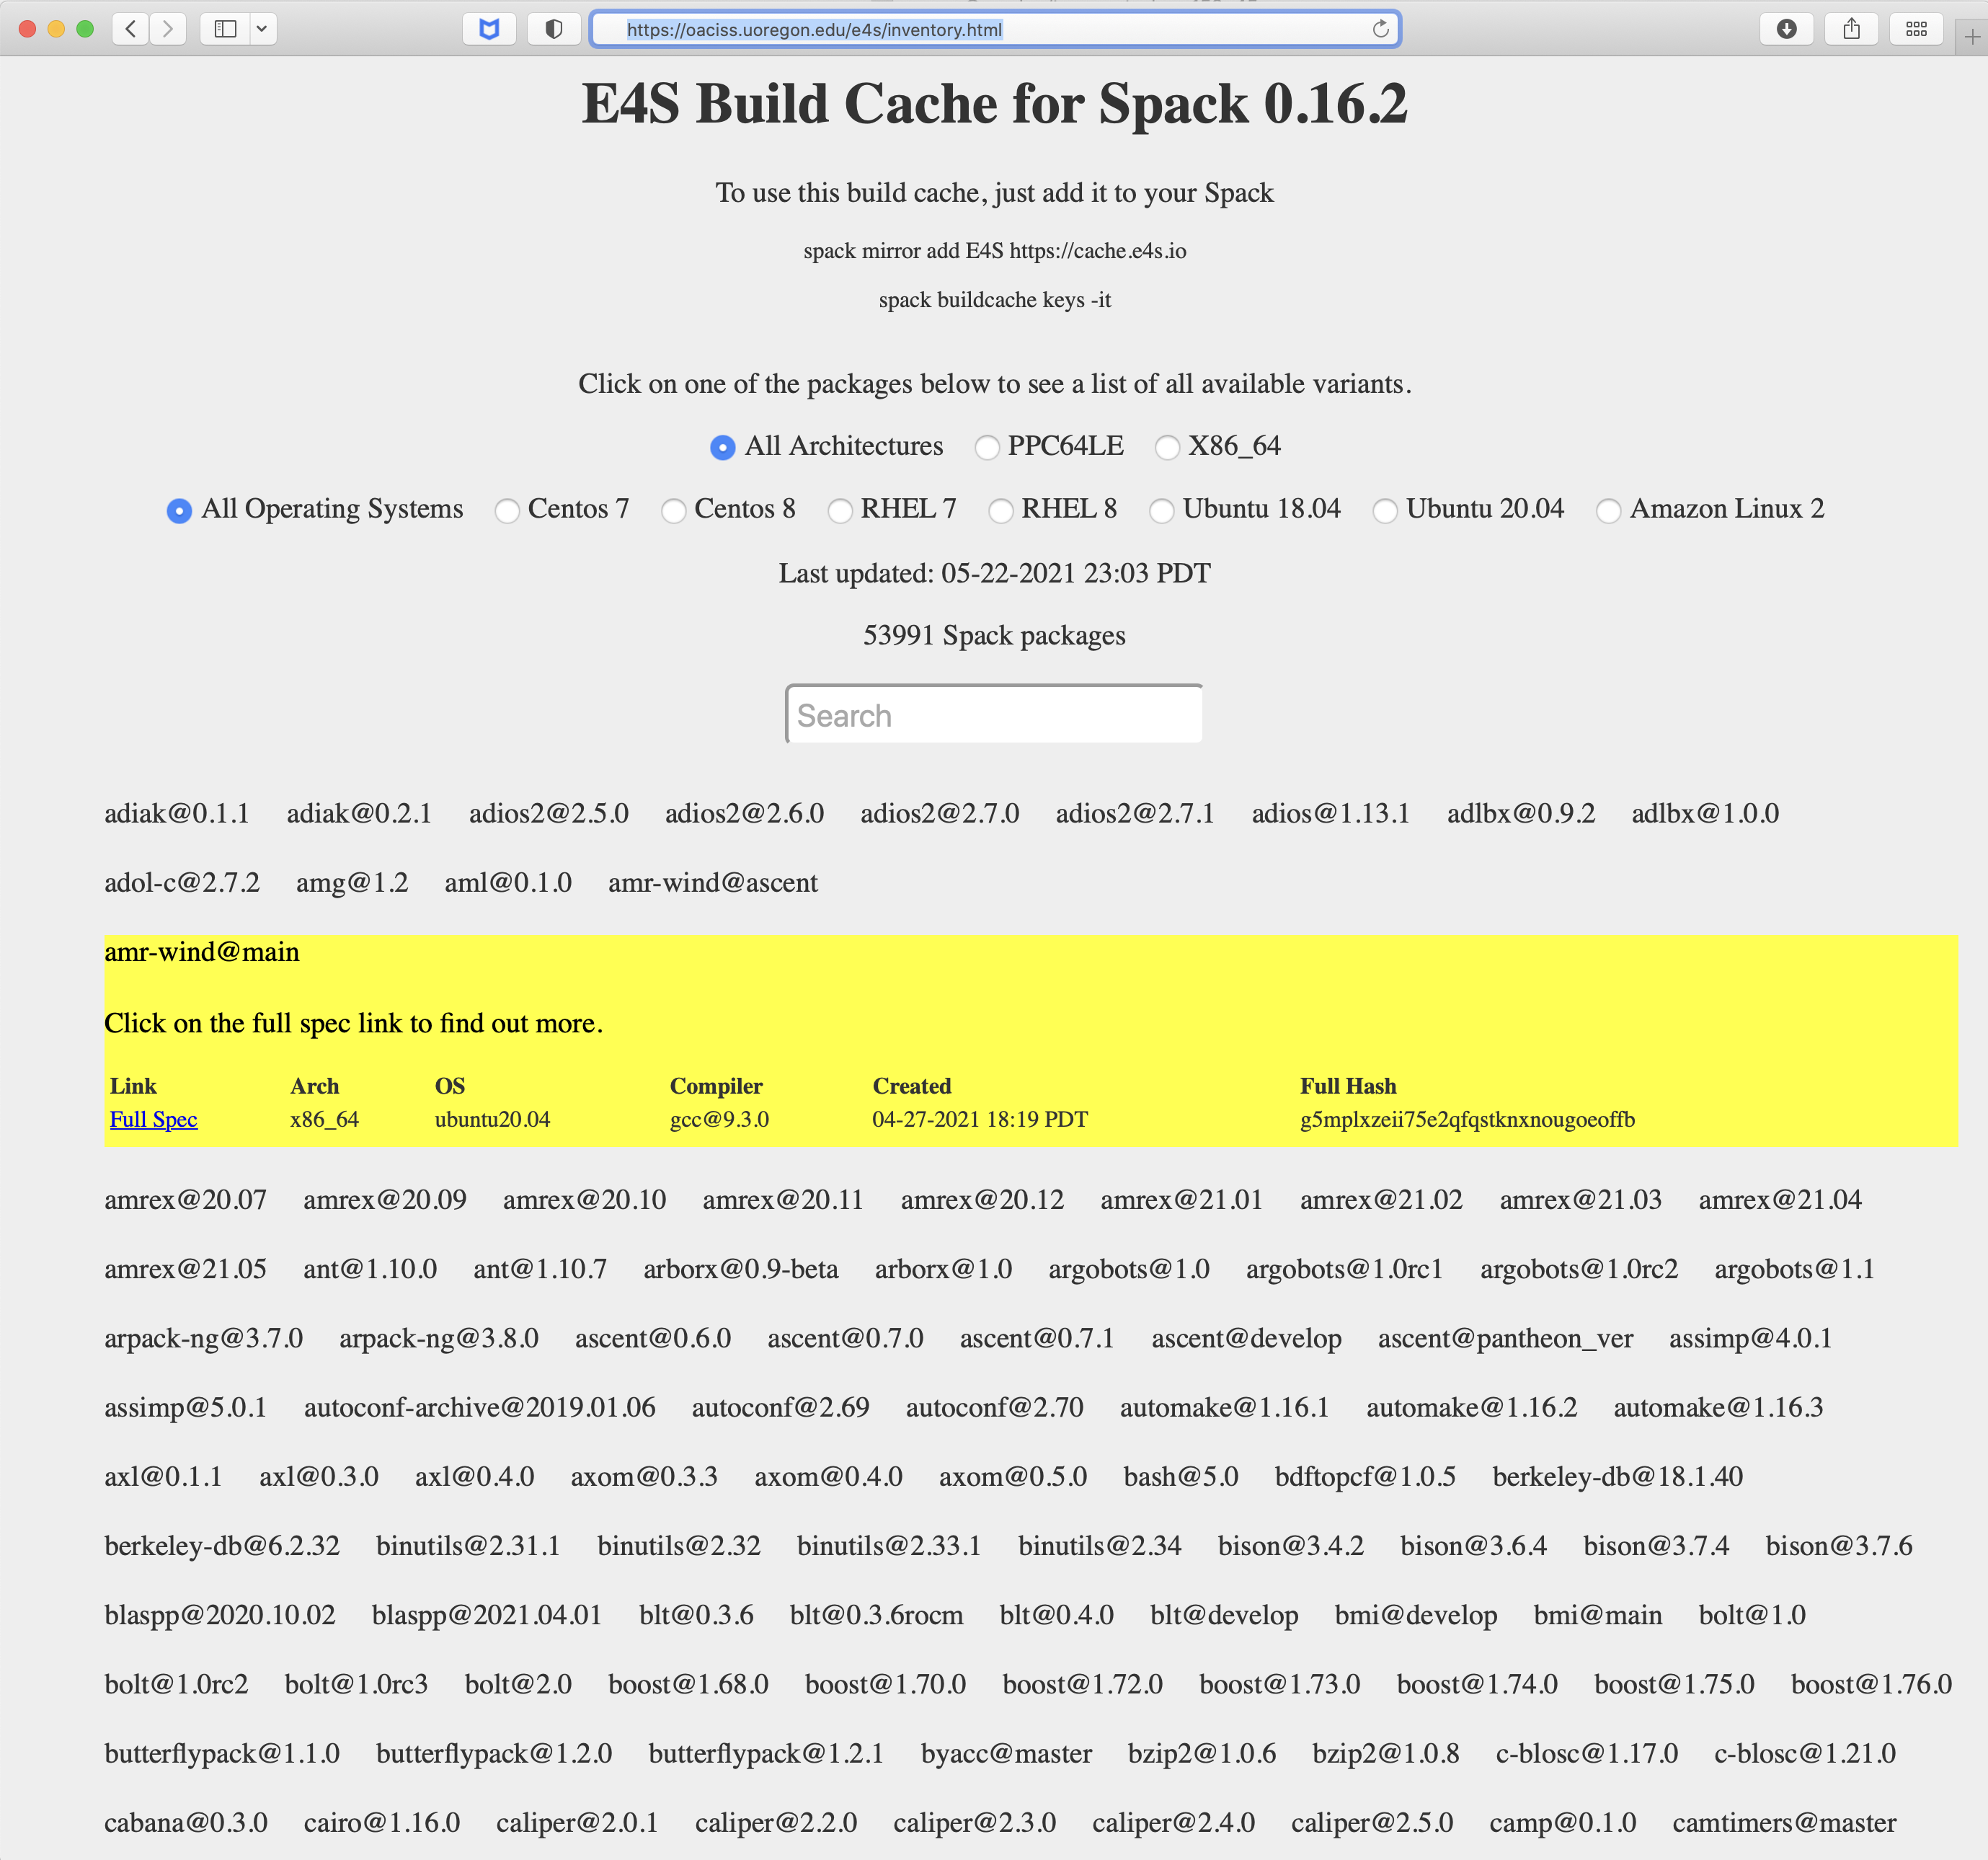
\includegraphics[width=0.9\linewidth]{projects/2.3.5-Ecosystem/2.3.5.01-Ecosystem-SDK/E4S_buildcache_Oct21}
	\caption{Using Spack build cache features, E4S builds can be accelerated via cached binaries for any build signature that Spack has already seen. Between September 2019 and September 2020, more than 21,000 binaries were added to the cache.}
	\label{fig:e4s-build-cache}
	\todo[inline]{Please add a ref to this figure in the narrative.}
\end{figure}

\begin{figure}
	\centering
	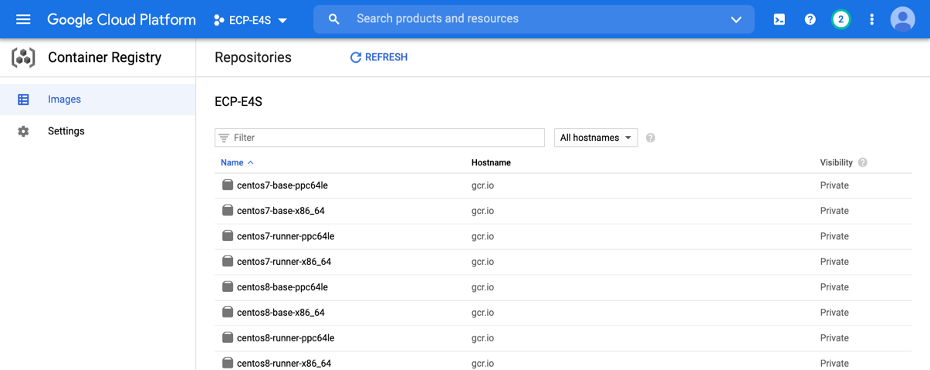
\includegraphics[width=0.9\linewidth]{E4S-GCP}
	\caption{E4S now supports Google Cloud Platform in addition to Amazon Web Services (AWS).}
	\label{fig:e4s-gcp-image}
	\todo[inline]{Please add a ref to this figure in the narrative.}
\end{figure}

The E4S effort is described in further detail in Sections~\ref{subsubsect:sdks} and~\ref{subsect:ecosystem}.

\subsubsection{Software Development Kits}\label{subsubsect:sdks}
One opportunity for a large software ecosystem project such as the ECP ST is to foster increased collaboration, integration, and interoperability among its funded efforts. Part of the ECP ST design is the creation of SDKs.  SDKs are collections of related software products, called \textit{packages}, in which coordination across package teams will improve usability and practices and foster community growth among teams that develop similar and complementary capabilities. SDKs have the following attributes.

\begin{enumerate}
	\item \textbf{Domain scope:} Each SDK will comprise packages whose capabilities are within a natural functionality domain. Packages within an SDK provide similar capabilities that can enable leveraging of common requirements, design, testing, and similar activities. Packages could have a tight complementary so that ready composability is valuable to the user.
	\item \textbf{Interaction models:} This is how packages within an SDK interact with each other. Interactions include common data infrastructure, or the seamless integration of other data infrastructures, and access to capabilities from one package for use in another.
	\item \textbf{Community policies:} These include expectations for how package teams will conduct activities, the services they provide, the software standards they follow, and other practices that can be commonly expected from a package in the SDK.
	\item \textbf{Meta-build system:} This includes robust tools and processes to build from source, install, and test the SDK with compatible versions of each package. This system sits on top of the existing build, install, and test capabilities for each package.
	\item \textbf{Coordinated plans:} Development plans for each package will include efforts to improve SDK capabilities and lead to better integration and interoperability.
	\item \textbf{Community outreach:} Efforts to reach out to the user and client communities will include explicit focus on SDK as a product suite.
\end{enumerate}
	
SDKs provide an aggregation of software products that have complementary or similar attributes. The ECP ST uses SDKs to better ensure product interoperability and compatibility.  SDKs are also essential aggregation points for coordinated planning and testing. SDKs are an integral element of the ECP ST~\cite{Heroux-SDK-Podcast}.  Section~\ref{subsubsect:ecosystem-sdk} describes the six SDK groupings and the current status of the SDK effort.
%\end{table}

\paragraph{ECP ST SDKs}
As part of the delivery of ECP ST capabilities, the team will establish and grow a collection of SDKs. The new layer of aggregation that SDKs represent is important for improving all aspects of product development and delivery. The communities that will emerge from SDK efforts will lead to better collaboration and higher quality products. Established community policies will provide a means to grow SDKs beyond the ECP to include any relevant external effort. The meta-build systems based on Spack will play an important role in managing the complexity of building the ECP ST software stack by providing a new layer in which versioning, consistency, and build options management can be addressed at a mid-scope below the global build of ECP ST products.
Each of the five ECP ST L3 has funds for an SDK project from which the team has identified six SDKs and an at-large collection of remaining products that will be delivered outside the SDK grouping.\todo{Per Julia, please clarify the preceding sentence.}  Section~\ref{subsubsect:ecosystem-sdk} provides an update on the progress in defining SDK groupings. For visibility, the same diagram is provided in Figure~\ref{fig:sdk-definition1-0}.

\begin{figure}[htb]
	\centering
	\fbox{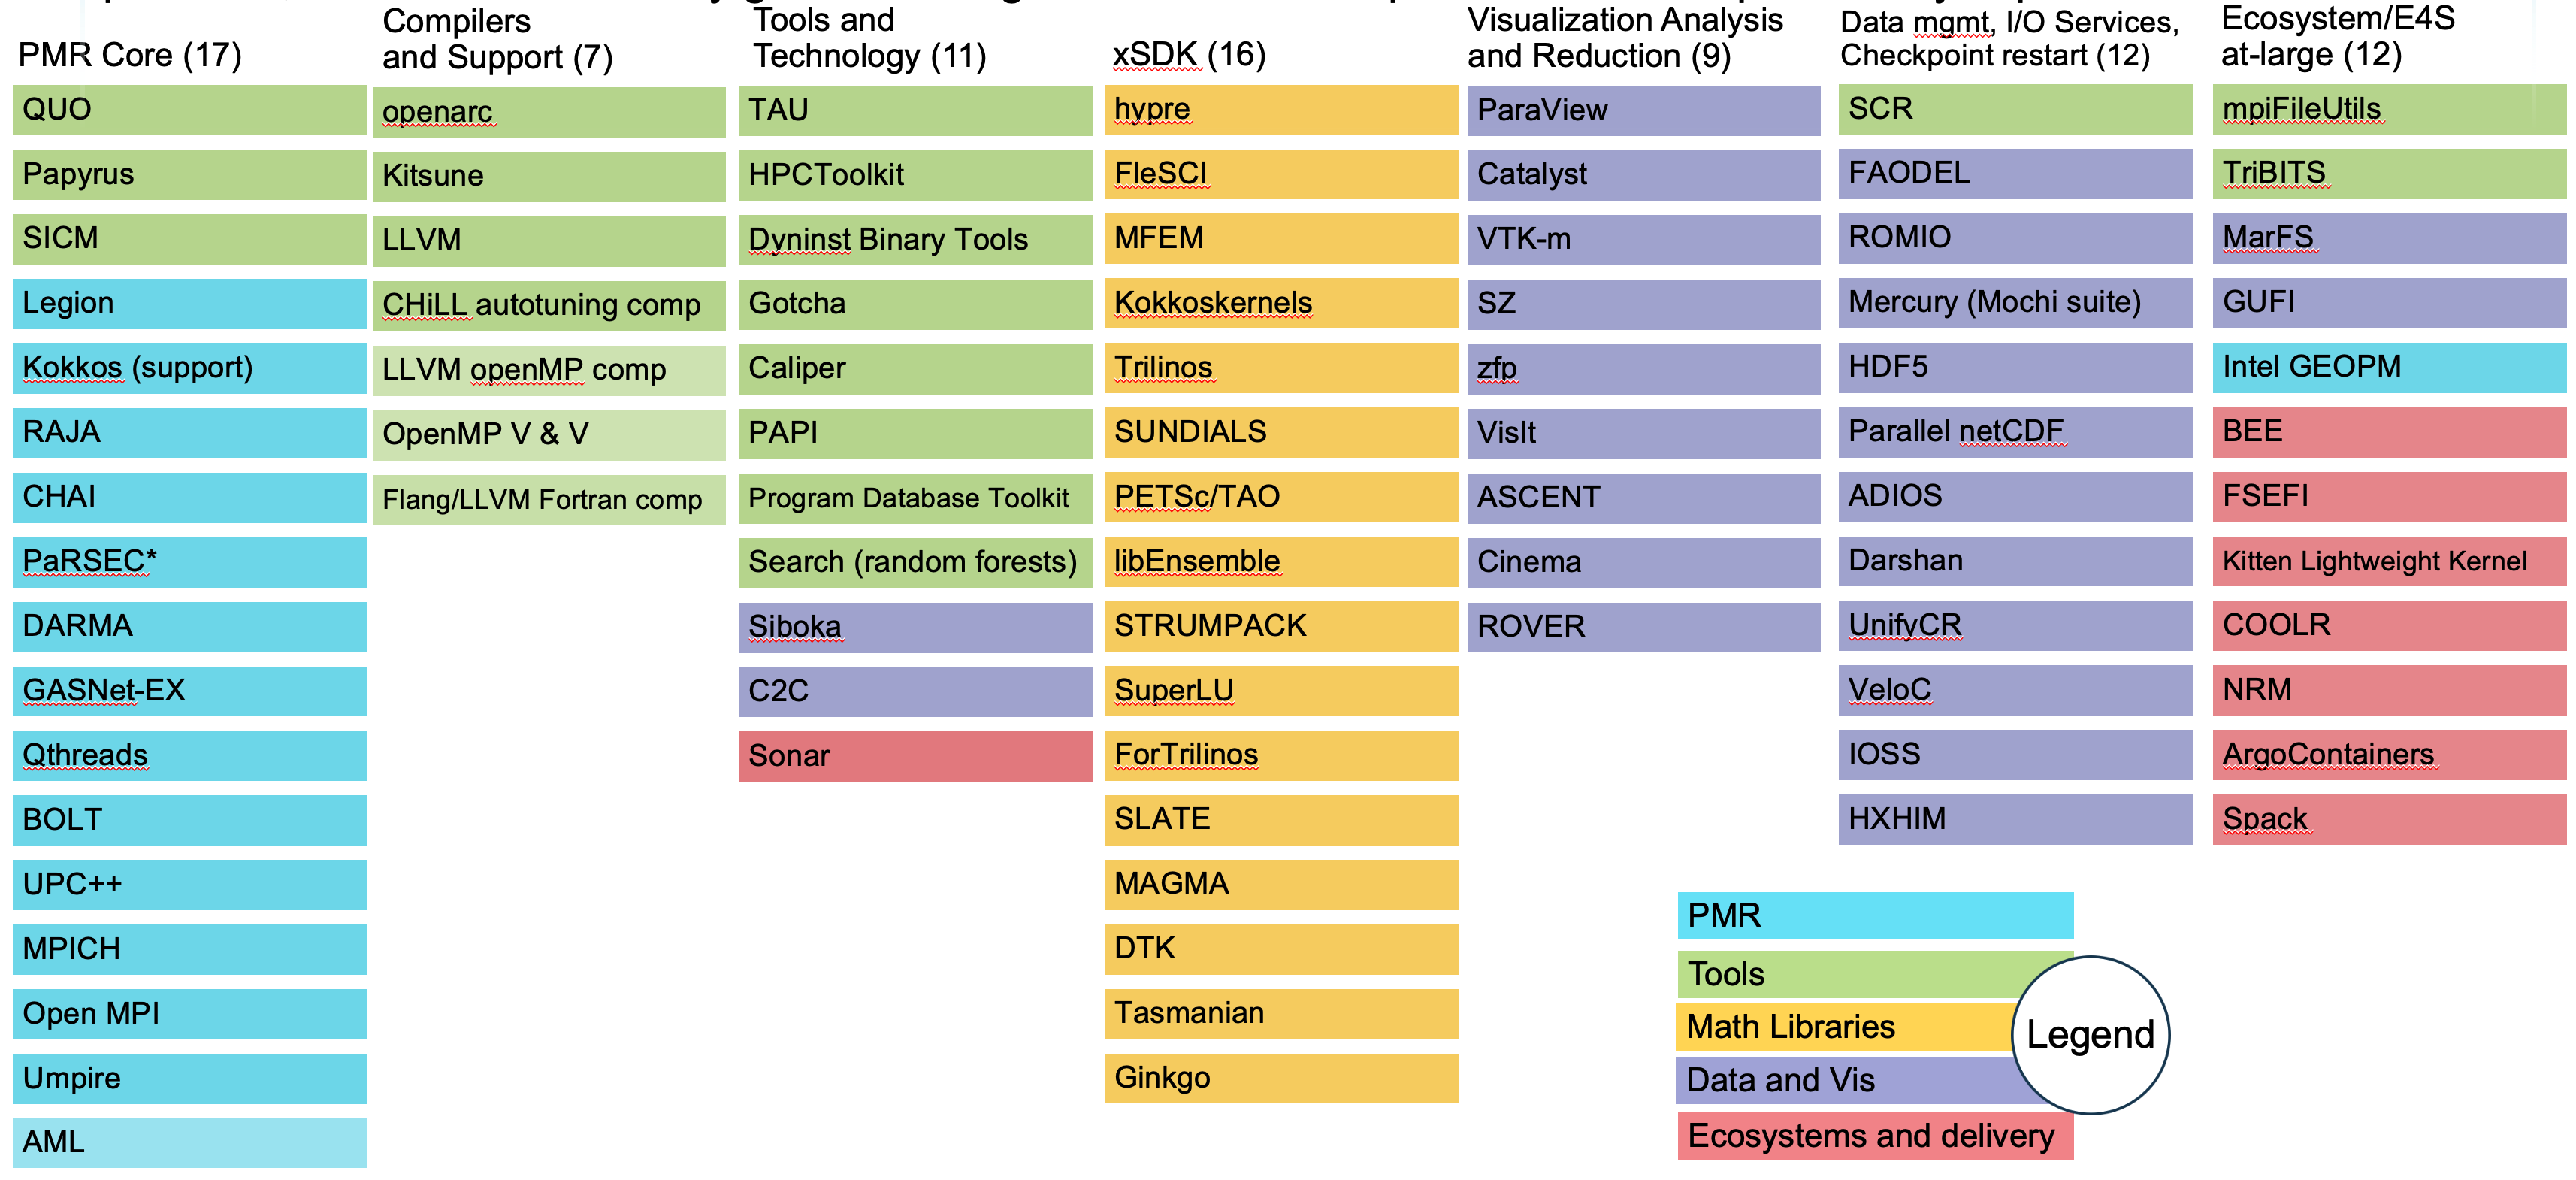
\includegraphics[width=6.5in]{projects/2.3.5-Ecosystem/2.3.5.01-Ecosystem-SDK/SDKdefinition3}}
	\caption{\label{fig:sdk-definition1-0}The breakdown of ECP ST products into six SDKs are shown in the first six columns. The rightmost column lists products that are not part of an SDK but are part of the Ecosystem group that will also be delivered as part of the E4S. The colors denoted in the key map all of the ST products sorted into their respective ST technical areas.  For example, the xSDK consists of products that are in the \mathlibs~technical area, plus TuckerMPI, which is in the \ecosystem~technical area.  Section~\ref{subsubsect:ecosystem-sdk} provides an update on the progress in defining SDK groupings.}
    \protect\todo[inline]{Please replace image with an image that is not a screenshot so that the image no longer has the red spellcheck underline.}
\end{figure}


\subsubsection{ECP ST Product Dictionary}\label{subsubsect:dictionary}
In the last year, the ECP has initiated an effort to explicitly manage ECP ST products and their dependencies (Section~\ref{subsubsect:dep-management}).  To eliminate ambiguities, a product dictionary---an official list of publicly named products to which ECP ST teams contribute their capabilities and upon which ECP ST clients depend---is needed.  The ECP product dictionary is one managed table that presently contains 70 primary products and subproducts that are either components within a product or particular implementations of a standard application programming interface (API).  Two special primary products are the Facilities stack and Vendor stack.  Having these stacks on the list enables ST teams to indicate that the team's capabilities are being delivered to ecosystems outside of the ECP.

Figure~\ref{fig:product-dictionary-overview} describes the policy for ECP ST teams to add and manage their contributions to the product dictionary.  Figure~\ref{fig:product-dictionary} shows a snapshot of the beginning and end of the current \textit{ECP ST Product Dictionary}, which is maintained on the ECP Confluence wiki. \todo{Is ``wiki" how it is listed in this document? If so, leave it. If not, please remove. Please make the same change in the caption of Figure 14.}

\begin{figure}
	\centering
	\fbox{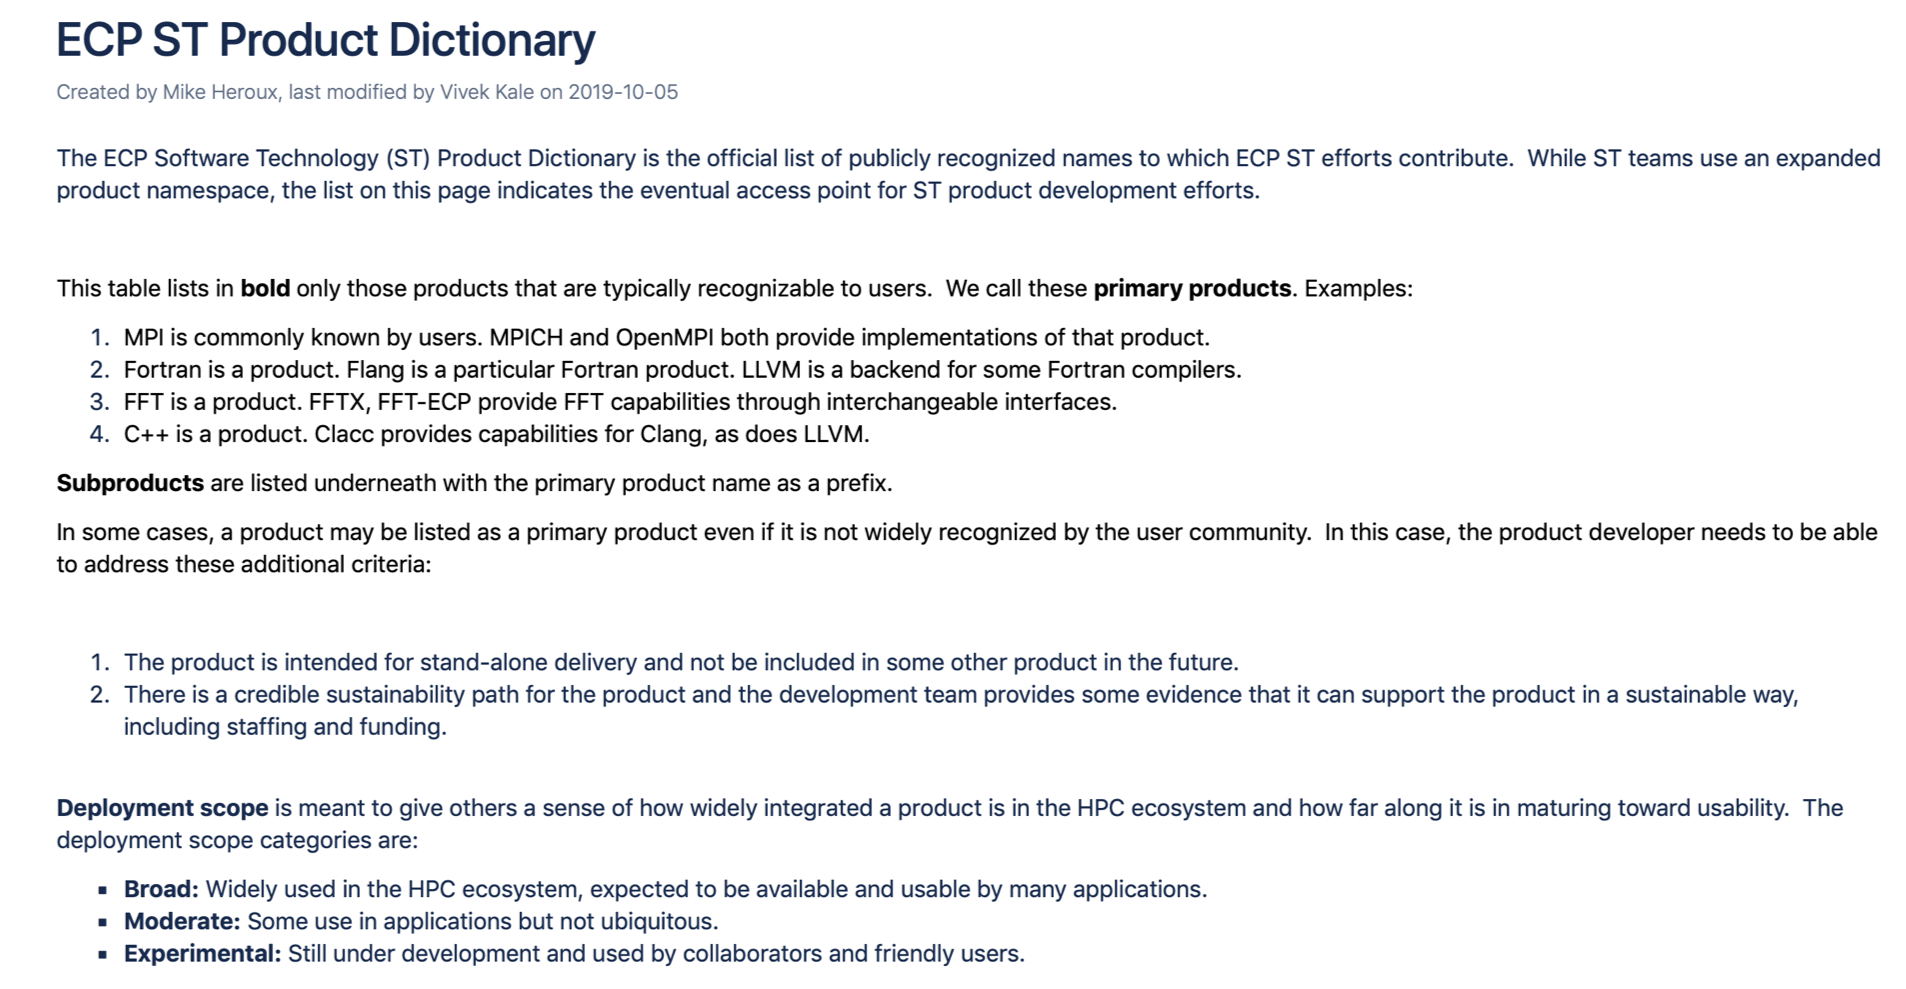
\includegraphics[width=0.9\linewidth]{ProductDictionaryOverview}}
	\caption{Screenshot from the top of the ECP Confluence wiki page containing the \textit{ECP ST Product Dictionary}.  The product dictionary structure contains primary and secondary products.  Client (i.e., consumer) dependencies are stated against the primary product names only, enabling unambiguous mapping of AD-on-ST and ST-on-ST dependencies.}
	\label{fig:product-dictionary-overview}
\end{figure}

\begin{figure}
	\centering
	\fbox{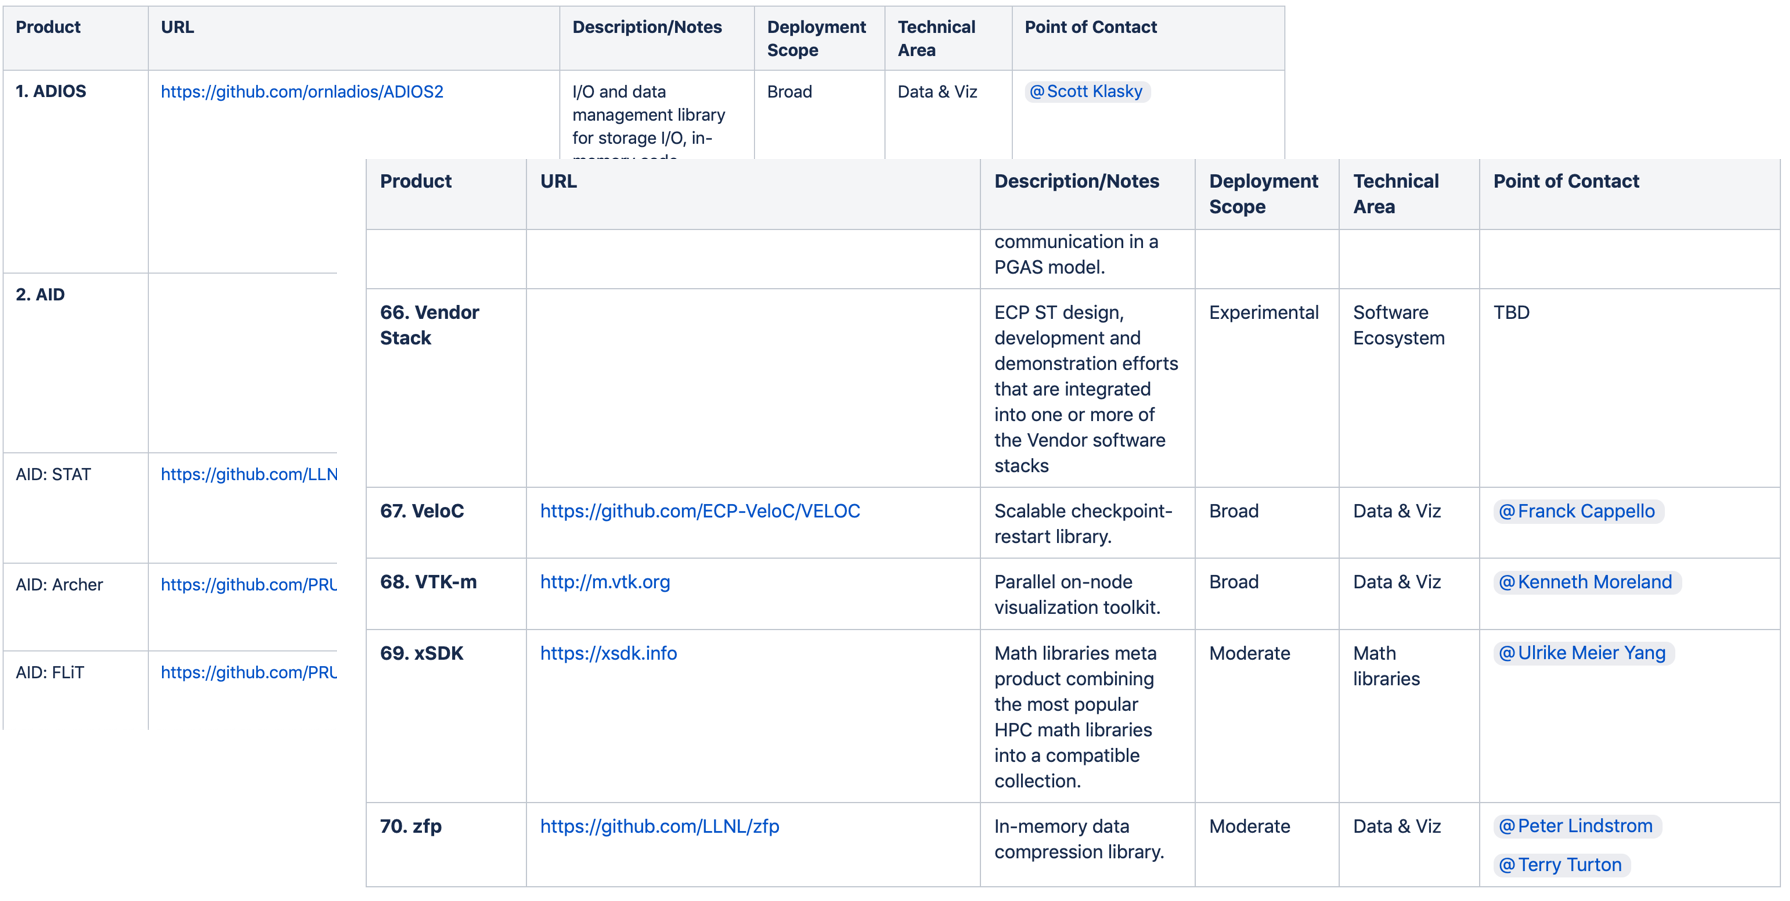
\includegraphics[width=0.9\linewidth]{ConfluenceProductDictionaryExample}}
	\caption{Screenshots of the \textit{ECP ST Product Dictionary} table.  The table is actively managed to include primary and secondary products to which the ECP ST team contributes and upon which ECP ST clients depend.  Presently, the product dictionary contains 70 primary products.  Secondary products are listed under the primary product with the primary product as a prefix.  For example, AID is the second primary product in the table shown here.  STAT, Archer, and FLIT are component subproducts.  MPI (not shown) is another primary product.  MPICH and OpenMPI are two robust MPI implementations and are listed as MPI subproducts.}
	\label{fig:product-dictionary}
\end{figure}

\subsubsection{ECP Product Dependency Management}\label{subsubsect:dep-management}
Given the \textit{ECP ST Product Dictionary} and a similar dictionary for ECP AD and co-design products, the ECP has created a dependency database that enables the creation and characterization of product-to-product dependencies. The ECP manages these dependencies in a Jira database by using a custom Jira issue type: Dependency.  The dependency database provides an important tool for understanding and managing ECP activities.  The dependency information is valuable within and outside the project.  Figure X \todo{Add figure number in place of X} shows a screenshot of the Jira dependency database dashboard, and Figure X \todo{Add figure number in place of X} shows a screenshot of an example query result in the Jira dependency database.

\begin{figure}
	\centering
	\fbox{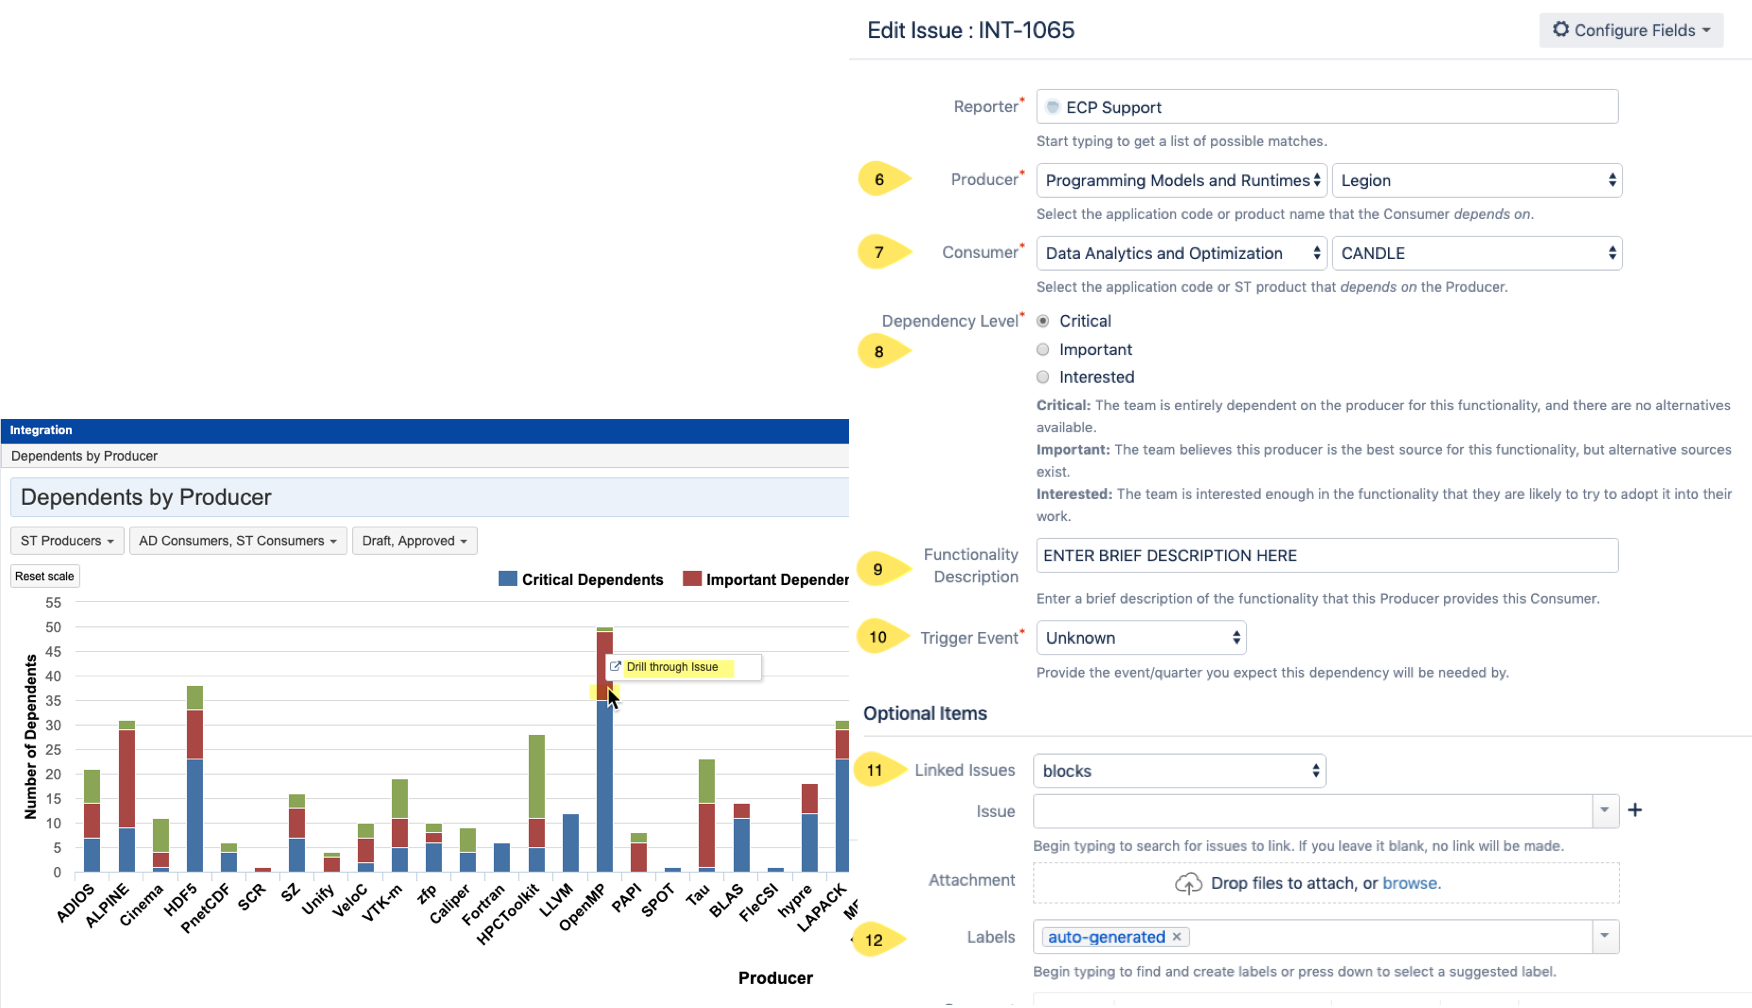
\includegraphics[width=0.9\linewidth]{DependencyDashboard-EditPanel}}
	\caption{Using Jira, the ECP manages its AD, ST, HI, vendor, and facilities dependencies.  This figure shows a screenshot of the Jira dependency database dashboard and an edit panel, which supports the creation and management of a consumer-on-producer dependency.}
	\label{fig:dependency-dashboard-edit}
	\todo[inline]{Please add a ref to this figure in the narrative.}
\end{figure}

\begin{figure}
	\centering
	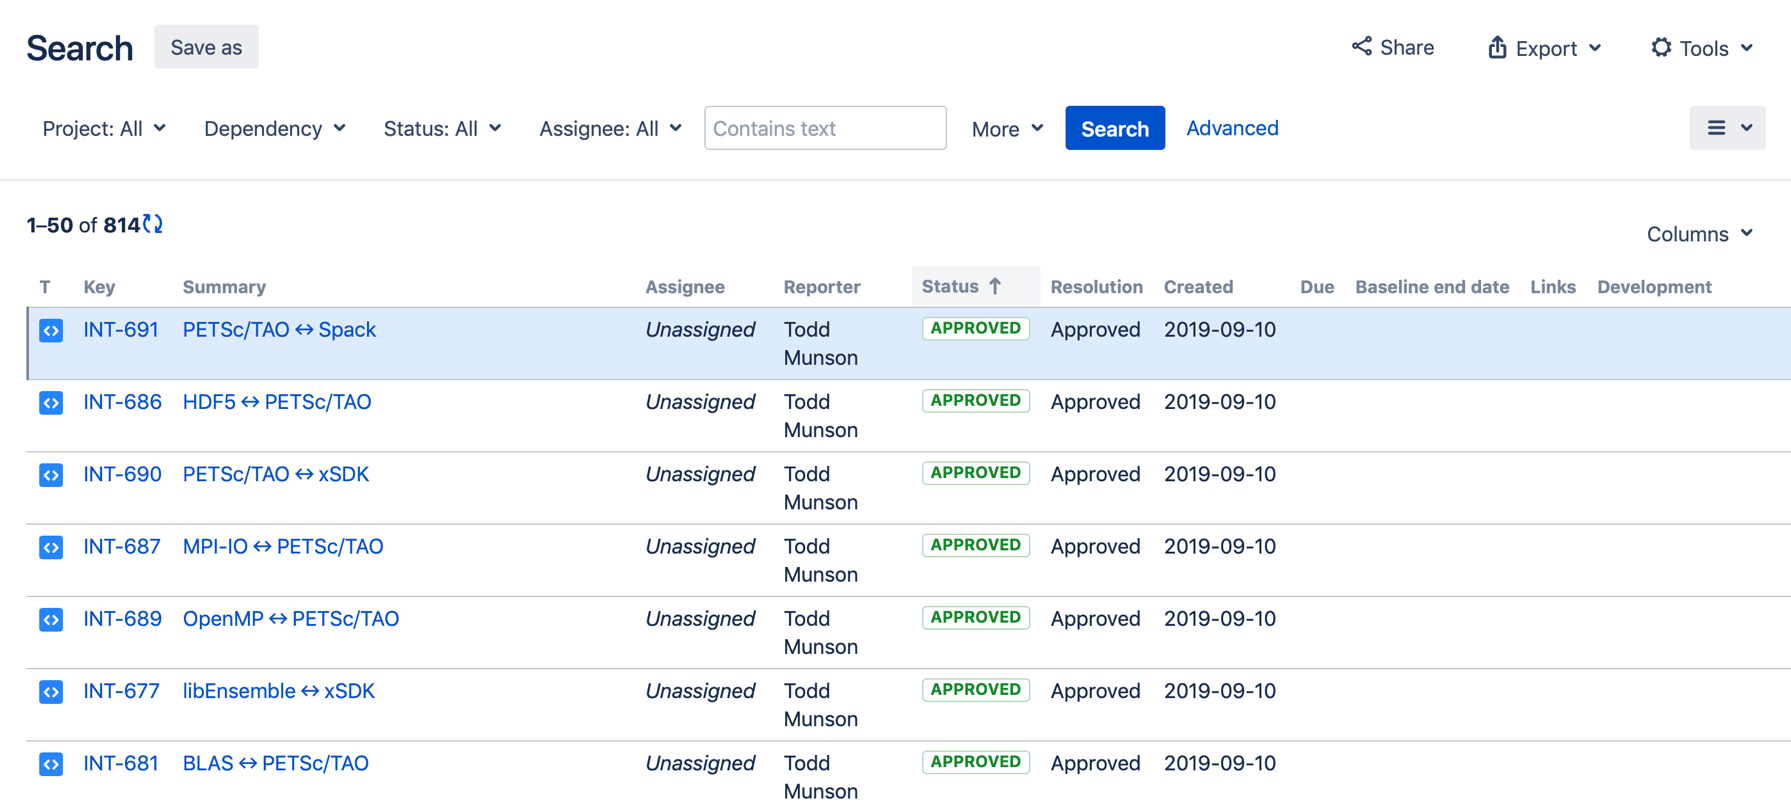
\includegraphics[width=0.9\linewidth]{PETSc-TAO-Dependencies}
	\caption{This query result from the ECP Jira dependency database lists all consumers of capabilities from the PETSc/TAO product. Selecting the details of one of the dependency issues shows how critical the dependency is and any custom information peculiar to the particular dependency.}
	\label{fig:petsc-tao-dependencies}
	\todo[inline]{Please add a ref to this figure in the narrative.}
\end{figure}

\newpage
\subsection{ECP ST Planning and Tracking}

Although the ECP is an official 413.3B federal construction project using an earned value management system, the ECP is permitted to tailor the planning process to obtain the flexibility needed for a software project, the requirements of which are emerging as the project proceeds.  This section describes how the ECP ST plans activities using the Jira project management tool.  The following sections discuss P6 activities, which are similar to milestones, and KPP-3, which is associated with the ECP ST.


\subsubsection{ECP ST P6 Activity Issues}

ECP ST uses a custom Jira issue type called \textit{P6 Activity}.  Each L4 subproject creates a series of P6 activity issues that extend to the end of the ECP (Q3 FY23).  Except for the current fiscal year, one P6 Activity issue describes expected deliverables as a planning package.  Six months before the start of a fiscal year, the planning package for the coming year is replaced with four to six issues that span the year with baseline start and end dates, an estimate of the percent annual budget and a high-level description.  Eight weeks before the start of an activity, full details about staffing, completion criteria, and more are added to the issue.  Figure~\ref{fig:planning-process} shows the steps in diagram form.  

Cost, scope, and schedule for the ECP ST are tracked and managed by monitoring the progress of the collection of P6 Activities.  Value is accrued when a P6 Activity issue is marked ``Done'' in the Jira database.  Schedule and cost performance indices are derived from the status of the P6 Activities.  Schedule, cost, and scope changes against the plan are managed via a formal project change request process.

\begin{figure}
	\centering
	\fbox{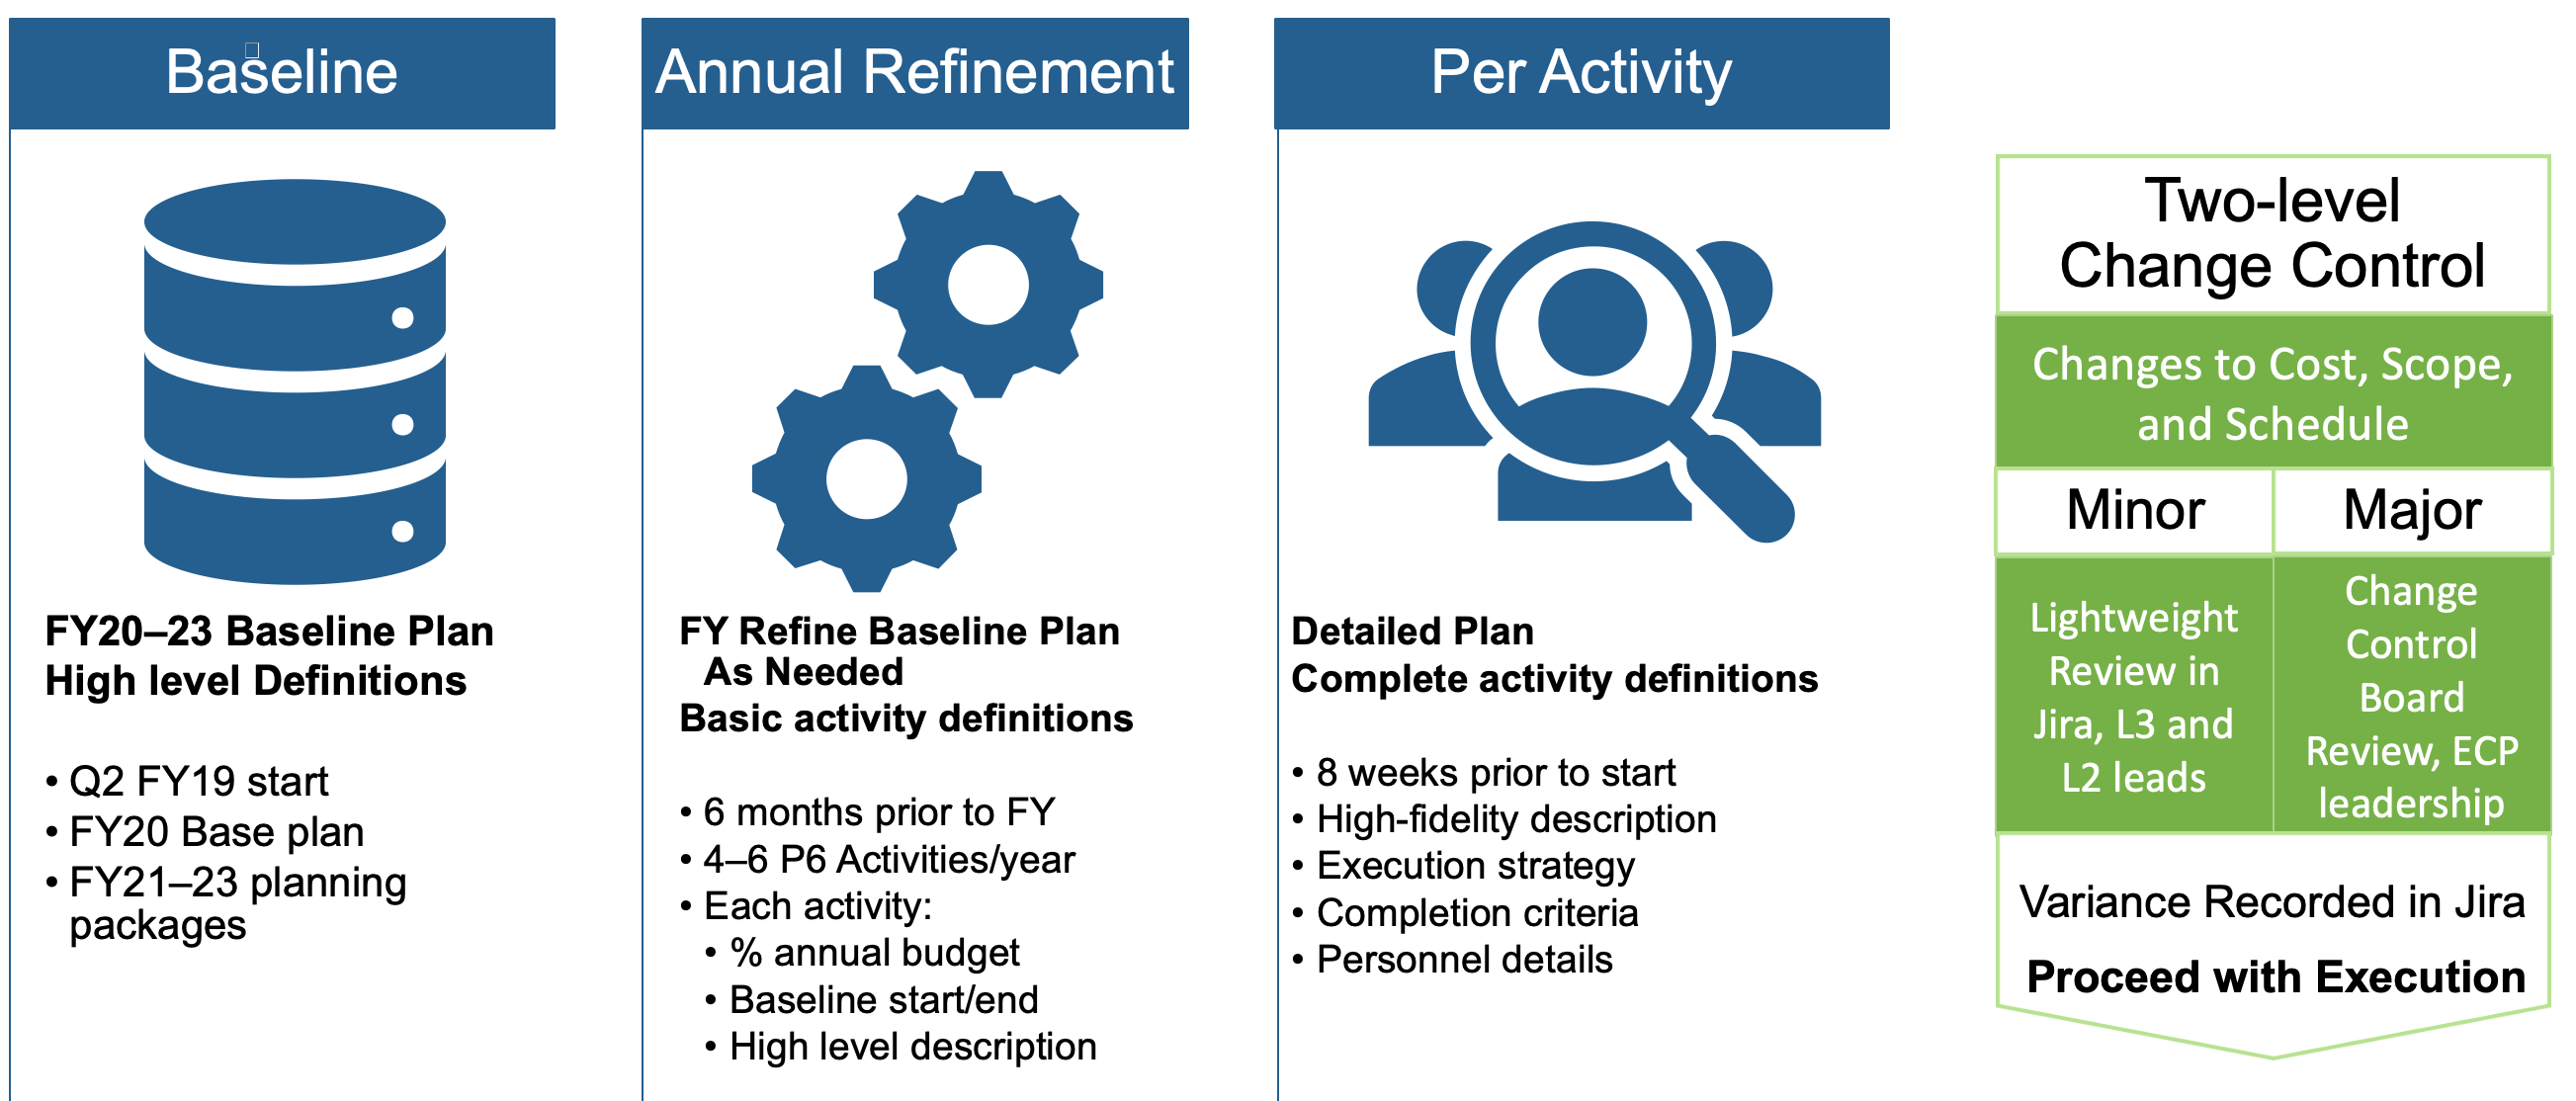
\includegraphics[width=0.9\linewidth]{Planning-Process}}
	\caption{Example of a P6 Activity.} 
	\protect\todo[inline]{The former caption was just repeating verbatim the previous paragraph. Please add a caption that describes what is shown in the image.}
	\label{fig:planning-process}
\end{figure}


\subsubsection{KPP-3}

The ECP has four KPPs.  Figure~\ref{fig:kpp-definitions} shows the KPP definitions. KPP-3 focuses on a productive and sustainable software ecosystem. The ECP ST is the primary owner of this KPP along with co-design projects in the ECP AD.  The focus of KPP-3 is to define and track capability integrations of ST products into the client environment, as described in this section. 

\begin{figure}
	\centering
	\fbox{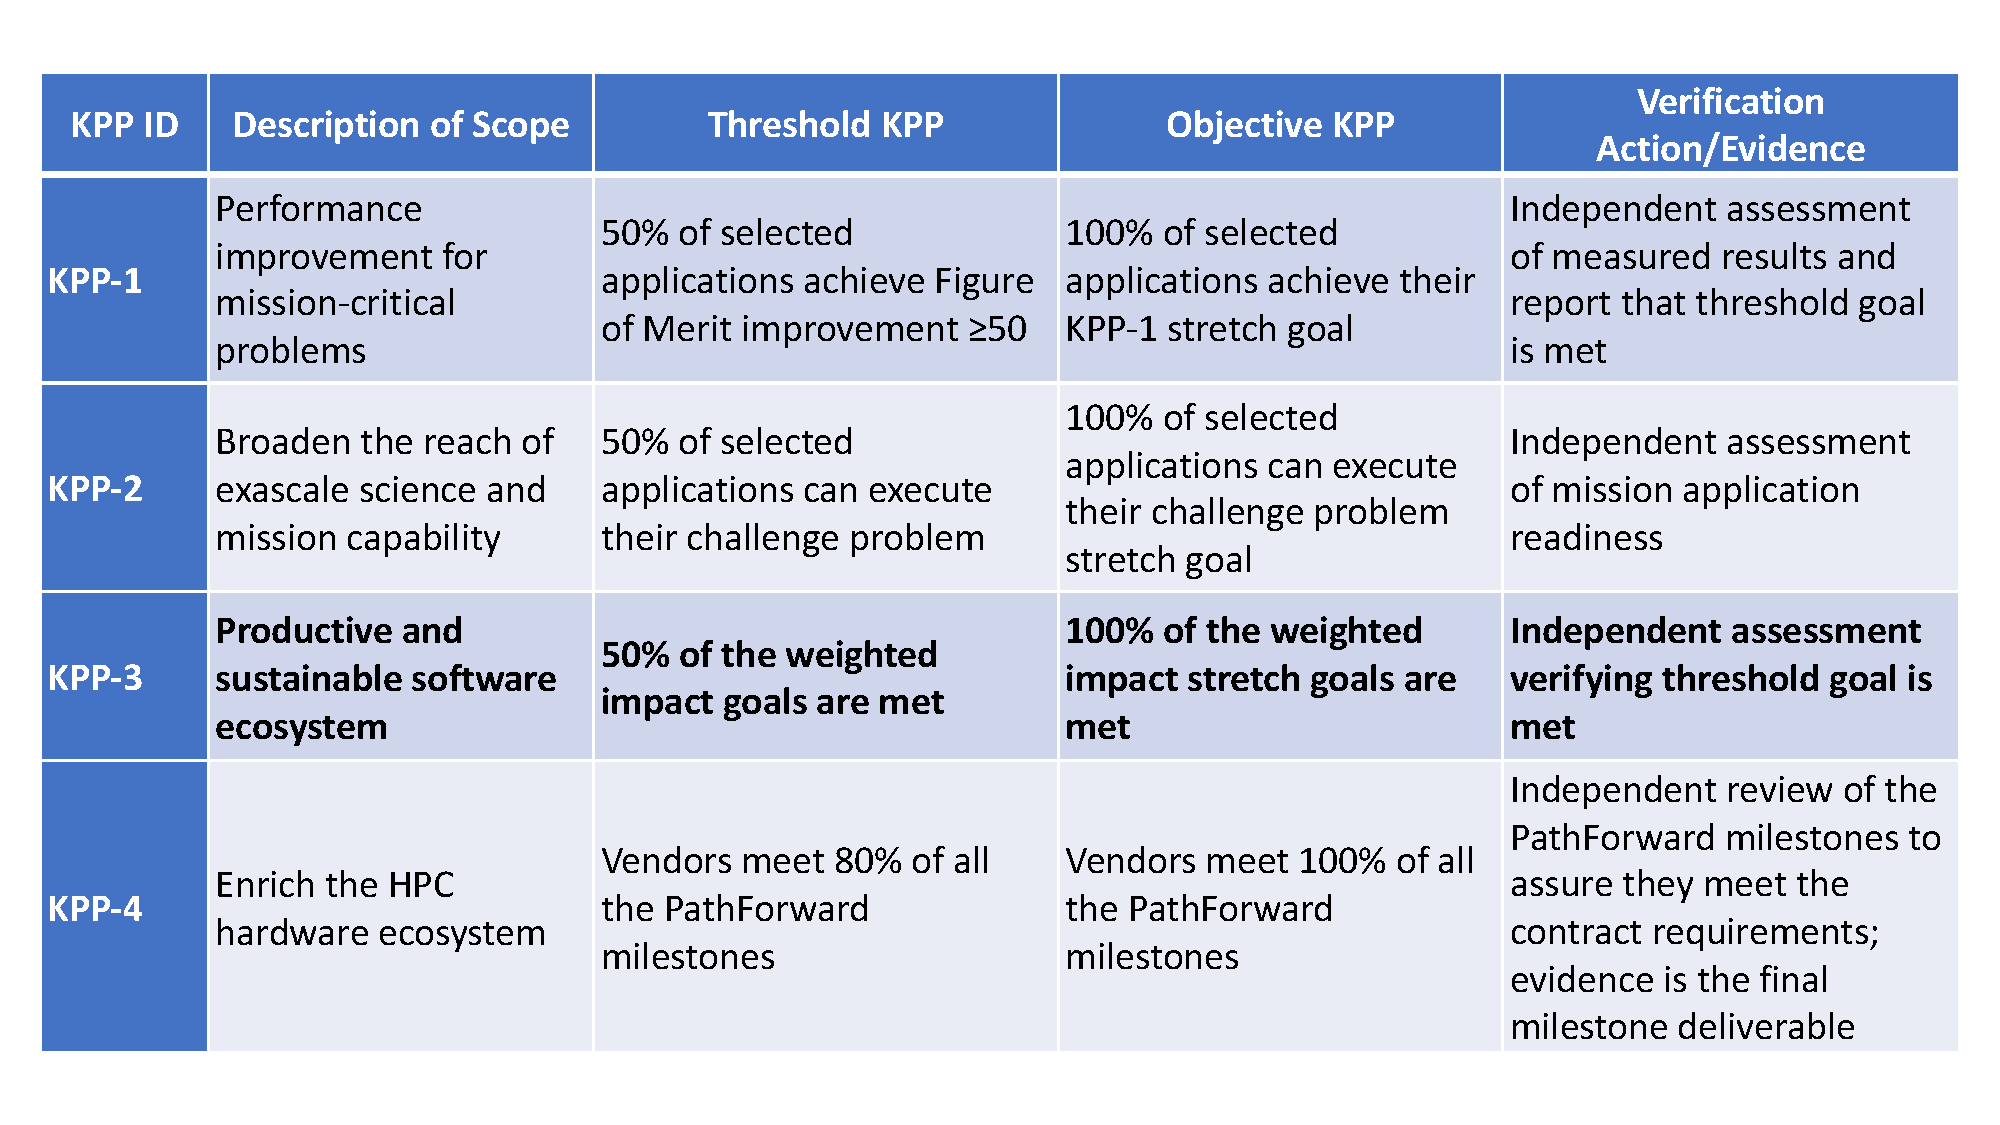
\includegraphics[width=0.9\linewidth]{KPP-Definitions}}
	\caption{The ECP's four KPPs.}
	\label{fig:kpp-definitions}
	\todo[inline]{Please convert this to an editable table or provide a higher-resolution version without blurry text.}
\end{figure}



The following terms are defined for clarity.
\begin{itemize}
	\item \textbf{Capability:} Any significant product functionality, including existing features adapted to the pre-exascale and exascale environments, that can be integrated into a client environment.
	\item \textbf{Integration goal:} A statement of impact on the ECP ecosystem in which a software capability is used in a consequential and sustainable way by a client in pre-exascale environments first, then in exascale environments.  Integration goals are product focused.  A project that contributes to more than one product will have a KPP-3 Jira issue for each of its products.
	\item \textbf{Integration score: }The number of successful capability integrations into a client environment (Table~\ref{table:KPP-3-scoring}).
	\item \textbf{Sustainable:} For KPP-3, \textit{sustainable} means that the capability is integrated in a way that reasonably ensures future use of the capability beyond the end of the ECP.  For libraries, \textit{sustainable} generally means that library usage is made from the source code in the main repository and use of the library is tested regularly as a part of the client code's regular regression testing.  For tools, \textit{sustainable} generally means that the tool is available as needed in the exascale environment.  For prototype capabilities that are incorporated into vendor and community software, the impact of the prototype is still visible to subject matter experts (SMEs).
\end{itemize}

\paragraph{Defining an Integration Goal:}
Integration goals are defined per product within each project.  The goal statement will include the following.
\begin{itemize}
	\item The name of the product to which the project contributes.  The product must be listed in the \textit{ECP ST Product Dictionary}.
	\item A description of the target clients' environments into which the product capabilities will be integrated.  Specific clients can be listed but are not necessary.  Clients must be part of the ECP or otherwise part of the exascale systems ecosystem, such as a vendor or facility partner.   
	\item A general description of the nature of the integration that addresses what it means to be successfully integrated.
\end{itemize}

\begin{table}[h!]
	\begin{tabular}{|L{1.5in}|L{2.0in}|L{2.5in}|}\hline
		\rowcolor{LightCyan}
		Integration score & Capability & Integration description\\\hline
		One point per capability sustainably integrated by a client per exascale platform used. &
		Complete, sustainable integration of a significant product capability into a client environment in a pre-exascale environment (tentative score) and in an exascale environment (confirmed score). &
		Clients acknowledge benefit from product capability use and considers it part of their workflow. Integration is sustainable with documentation and testing. Integration of product capability into main product repo and SDK/E4S environments is completed.\\\hline
	\end{tabular}
	\caption{\label{table:KPP-3-scoring} Integration goal scoring. One point is accrued when a client integrates and sustainably uses a product's capabilities.  Scores are assessed annually.}
\end{table}


\paragraph{Demonstrating and Recording Progress toward an Integration Goal:}
All artifacts and evidence of progress will be captured in the Jira KPP-3 issue associated with a product integration goal as progress is made.  All integration scores are tentative until the capability is available and demonstrated in exascale environments.  Table~\ref{table:KPP-3-values} summarizes the defined values.

\begin{table}[h!]
	\begin{tabular}{|L{0.6in}|L{2.0in}|L{3.4in}|}\hline
		\rowcolor{LightCyan}
		Value & Definition & Description\\\hline
		Present & The current integration score. & This is always an indication of the progress that the team has made. The present value is assessed annually.\\\hline
		Passing & The minimum integration score required for the product to be counted as part of ECP ST progress toward KPP-3. & The passing score is between 4 and 8 for each integration goal, in which 4 is for larger integration efforts, and 8 is for smaller ones. This is equivalent to accomplishing one to two capability integrations per year, per product.\\\hline
		Stretch & The maximum reasonably achievable integration score for a product if capability integrations are successful with all potential ECP clients.   & The stretch value shows the overall integration potential.\\\hline
	\end{tabular}
	\caption{\label{table:KPP-3-values} Key metric values. These values are determined by the L4 subproject team when defining its KPP-3 issue.}
\end{table}

\paragraph{Assessment Process:}
Although progress is recorded as it is achieved, progress assessment is done annually, including input from external SMEs.  ECP leadership and SMEs will review integration score evidence, confirming or adjusting integration scores.
Assessments can result in a reduced integration score from a previous year if a client has stopped using a capability that was previously used.

\paragraph{Transition from Tentative to Confirmed Integration Score:}
Each integration score is tentative until the capability is available and demonstrated to be effective in the exascale environments.  Demonstration can be achieved in a variety of ways so that ECP leadership and SMEs are reasonably certain that the capability positively impacts the client in exascale environments.  At this point, the integration score becomes confirmed. 
Typically, the transition from tentative to confirmed would be a low-cost, independent demonstration or accomplished within the client’s environment as the client is conducting its own assessments. 
The planned exascale system, El Capitan, that can support National Security Applications will not be available until the end of FY23. Integrating ST products into National Security Applications will be considered for transition from tentative to confirmed when: (1) evidence of integration is provided during FY20--22 ASC L1 and L2 milestones related to ECP/ATDM National Security Application readiness for exascale platforms and/or (2) integration is demonstrated on the El Capitan early access systems and exercises capabilities similar to those anticipated to be important for effectively using El Capitan.  For KPP-3 capability integrations targeted at El Capitan, the ECP will use the best available confirmation process in FY23. Table~\ref{table:KPP-3-impact} explains the weight of the integration scores. 


\begin{table}[h!]
	\begin{tabular}{|L{1.0in}|L{0.5in}|L{4.5in}|}\hline
		\rowcolor{LightCyan}
		Impact level & Weight & Comments\\\hline
		High & 2 & The score for integration goals associated with high-impact products will be added to the KPP-3 score with a weight of 2.\\\hline
		Normal & 1 & Most KPP-3 Jira issues will have a weight of 1.\\\hline
		Risk mitigating & 0.5 & Some KPP-3 Jira issues are associated with products that help plan for the potential risks if high-impact products do not deliver as expected.\\\hline
		Shared  & 0.5 & Some projects receive funding from both NNSA and DOE SC (e.g., RAJA/Kokkos). For these projects, the score is balanced to reflect dual contributions.\\\hline
	\end{tabular}
	\caption{\label{table:KPP-3-impact} Integration scores. Each integration score will have an associated weight, depending on the potential impact if integration targets are not met.}
\end{table}

The KPP-3 score is the weighted sum of all integration goals that have an integration score that meets or exceeds its passing value. 
The KPP-3 score will initially be tentative.  The KPP-3 score is not officially met until the weighted sum of confirmed integration scores exceeds 50\% of the total possible points.


\subsubsection{ECP ST Software Delivery}
One essential activity for---and the ultimate purpose of---ECP ST is the delivery of a software stack that enables productive and sustainable exascale computing capabilities for target ECP applications and platforms and the broader HPC community. The ECP ST Software Ecosystem and Delivery sub-element (WBS 2.3.5), and the SDKs in each sub-element, provide the means by which the ECP ST will deliver its capabilities.
\paragraph{ECP ST Delivery and HI Deployment:}
Providing the ECP ST software stack to ECP applications requires coordination between the ECP ST and ECP HI. The focus areas have a complementary arrangement in which the ECP ST delivers its products, and the ECP HI deploys them. The process is described specifically as follows.
\begin{itemize}
	\item The ECP ST delivers software.  ECP ST products are delivered directly to application teams, vendors, and facilities.  The ECP ST designs and implements products to run on DOE computing facilities platforms and make products available as source code via GitHub, GitLab, or another accessible repository.
	\item The ECP HI facilitates efforts to deploy ST and other software on facilities platforms by installing them where users expect to find them. This could be in \texttt{/usr/local/bin} or a similar directory or available via ``module load.''
\end{itemize}
Separating the concerns of delivery and deployment is essential because these activities require different skill sets. Furthermore, the ECP ST delivers its capabilities to an audience that is beyond the scope of specific facilities’ platforms. This broad scope is essential for the sustainability of ECP ST products, expanding the user and developer communities needed for vitality. Additionally, the ECP HI, computer system vendors, and other parties provide deployable software outside the scope of the ECP ST, thus having the critical skills needed to deploy the entire software stack.

\paragraph{ECP ST Delivery Strategy:}
The ECP ST delivers its software products as source code, primarily in repositories found on GitHub or GitLab installations or similar platforms. Clients such as the ECP HI, OpenHPC, and application developers with direct repository access then take the source and build, install, and test the ECP ST software. The delivery strategy is outlined in Figure~\ref{fig:hierarchy}, and  
%
users access ECP ST products using the following basic mechanisms.
\begin{itemize}
	\item \textbf{Build from source code:} Most ECP ST products reach at least some of their user base via direct source code download from the product repository.  In some cases, users download one compressed file that contains the product source, then expand the file to expose the collection of source and build files.  Increasingly, users will fork a new copy of an online repository.  After obtaining the source, users execute a configuration process that detects local compilers and libraries and then builds the product.  This kind of access can be a barrier for some users because users need to build the product and can encounter a variety of challenges in that process, such as an incompatible compiler or a missing third-party library that must first be installed.  However, building from the source can be a preferred approach for users who want control over compiler settings or want to adapt how the product is used (e.g., turning on or off optional features, creating adaptations that extend product capabilities). For example, large library frameworks, such as PETSc and Trilinos, have many tunable features that can benefit from users building from source code.  Furthermore, these frameworks support user-defined functional extensions that are easier to support when users builds the product from source. The ECP ST is leveraging and contributing to the development of Spack~\cite{gamblin+:sc15}.  Via metadata stored in a Spack package defined for each product, Spack leverages a product's native build environment, along with knowledge about its dependencies, to build the product and dependencies from source.  Spack plays a central role in ECP ST software development and delivery processes by supporting turnkey builds of the ECP ST software stack for the purposes of continuous integration testing, installation, and seamless multiproduct builds.
	\item \textbf{DOE computing facilities:} Each DOE computing facility---Argonne Leadership Computing Facility (ALCF), Oak Ridge Leadership Computing Facility (OLCF), National Energy Research Scientific Computing Center (NERSC), LLNL, and the Atmosphere, Climate, and Ecosystem Science (ACES) collaboration (Los Alamos National Laboratory [LANL] and Sandia National Laboratories~[SNL]) provides pre-built versions of 17--20 ECP ST products, although the exact mix of products varies somewhat at each site. Many of these products are what users would consider to be part of the core system capabilities, including compilers---such as Flang (Section~\ref{subsubsect:flang}) and LLVM (Section~\ref{subsubsect:sollve})---and parallel programming environments, such as MPICH (Section~\ref{subsubsect:mpich}), OpenMPI (Section~\ref{subsubsect:openmpi}), and OpenMP (Section~\ref{subsubsect:bolt}).  Development tools, such as PAPI (Section~\ref{subsubsect:exapapi}) and TAU (Section~\ref{subsubsect:tau}), are often part of this suite if they are not already included in the vendor stack. Math and data libraries, such as PETSc (Section~\ref{subsubsect:petsc}), Trilinos (Section~\ref{subsubsect:peeks}), HDF5 (Section~\ref{subsubsect:exahdf5}), and others are also available in some facilities' software installations. The team anticipates and hopes for increased collaboration with facilities via the ECP HI focus area.  The team is also encouraged by multi-lab efforts, such as the Tri-Lab Operating System Stack (TOSS)~\cite{TOSS}, that are focused on improving the uniformity of software stacks across facilities.
	\item \textbf{Vendor stacks:} Computer system vendors leverage DOE investments in compilers, tools, and libraries.  Of particular note is the wide use of MPICH~(Section~\ref{subsubsect:mpich}) as a software base for most HPC vendor MPI implementations and the requirements, analysis, design, and prototyping that ECP ST teams provide.  Section~\ref{subsection:external-contributions} describes some of these efforts.
	\item \textbf{Binary distributions:} Approximately 10 ECP ST products are available via binary distributions, such as common Linux distributions, particularly via OpenHPC~\cite{OpenHPC}. The ECP ST intends to foster the growth of availability via binary distributions as an important way to increase the size of the user community and improve product sustainability via this broader user base.  
	\item \textbf{Container and cloud environments:} E4S is available via an increasing number of container and cloud environments, such as Docker, Shifter, Singularity, CharlieCloud, AWS, and Google Cloud.
\end{itemize}

\begin{figure}
	\centering
	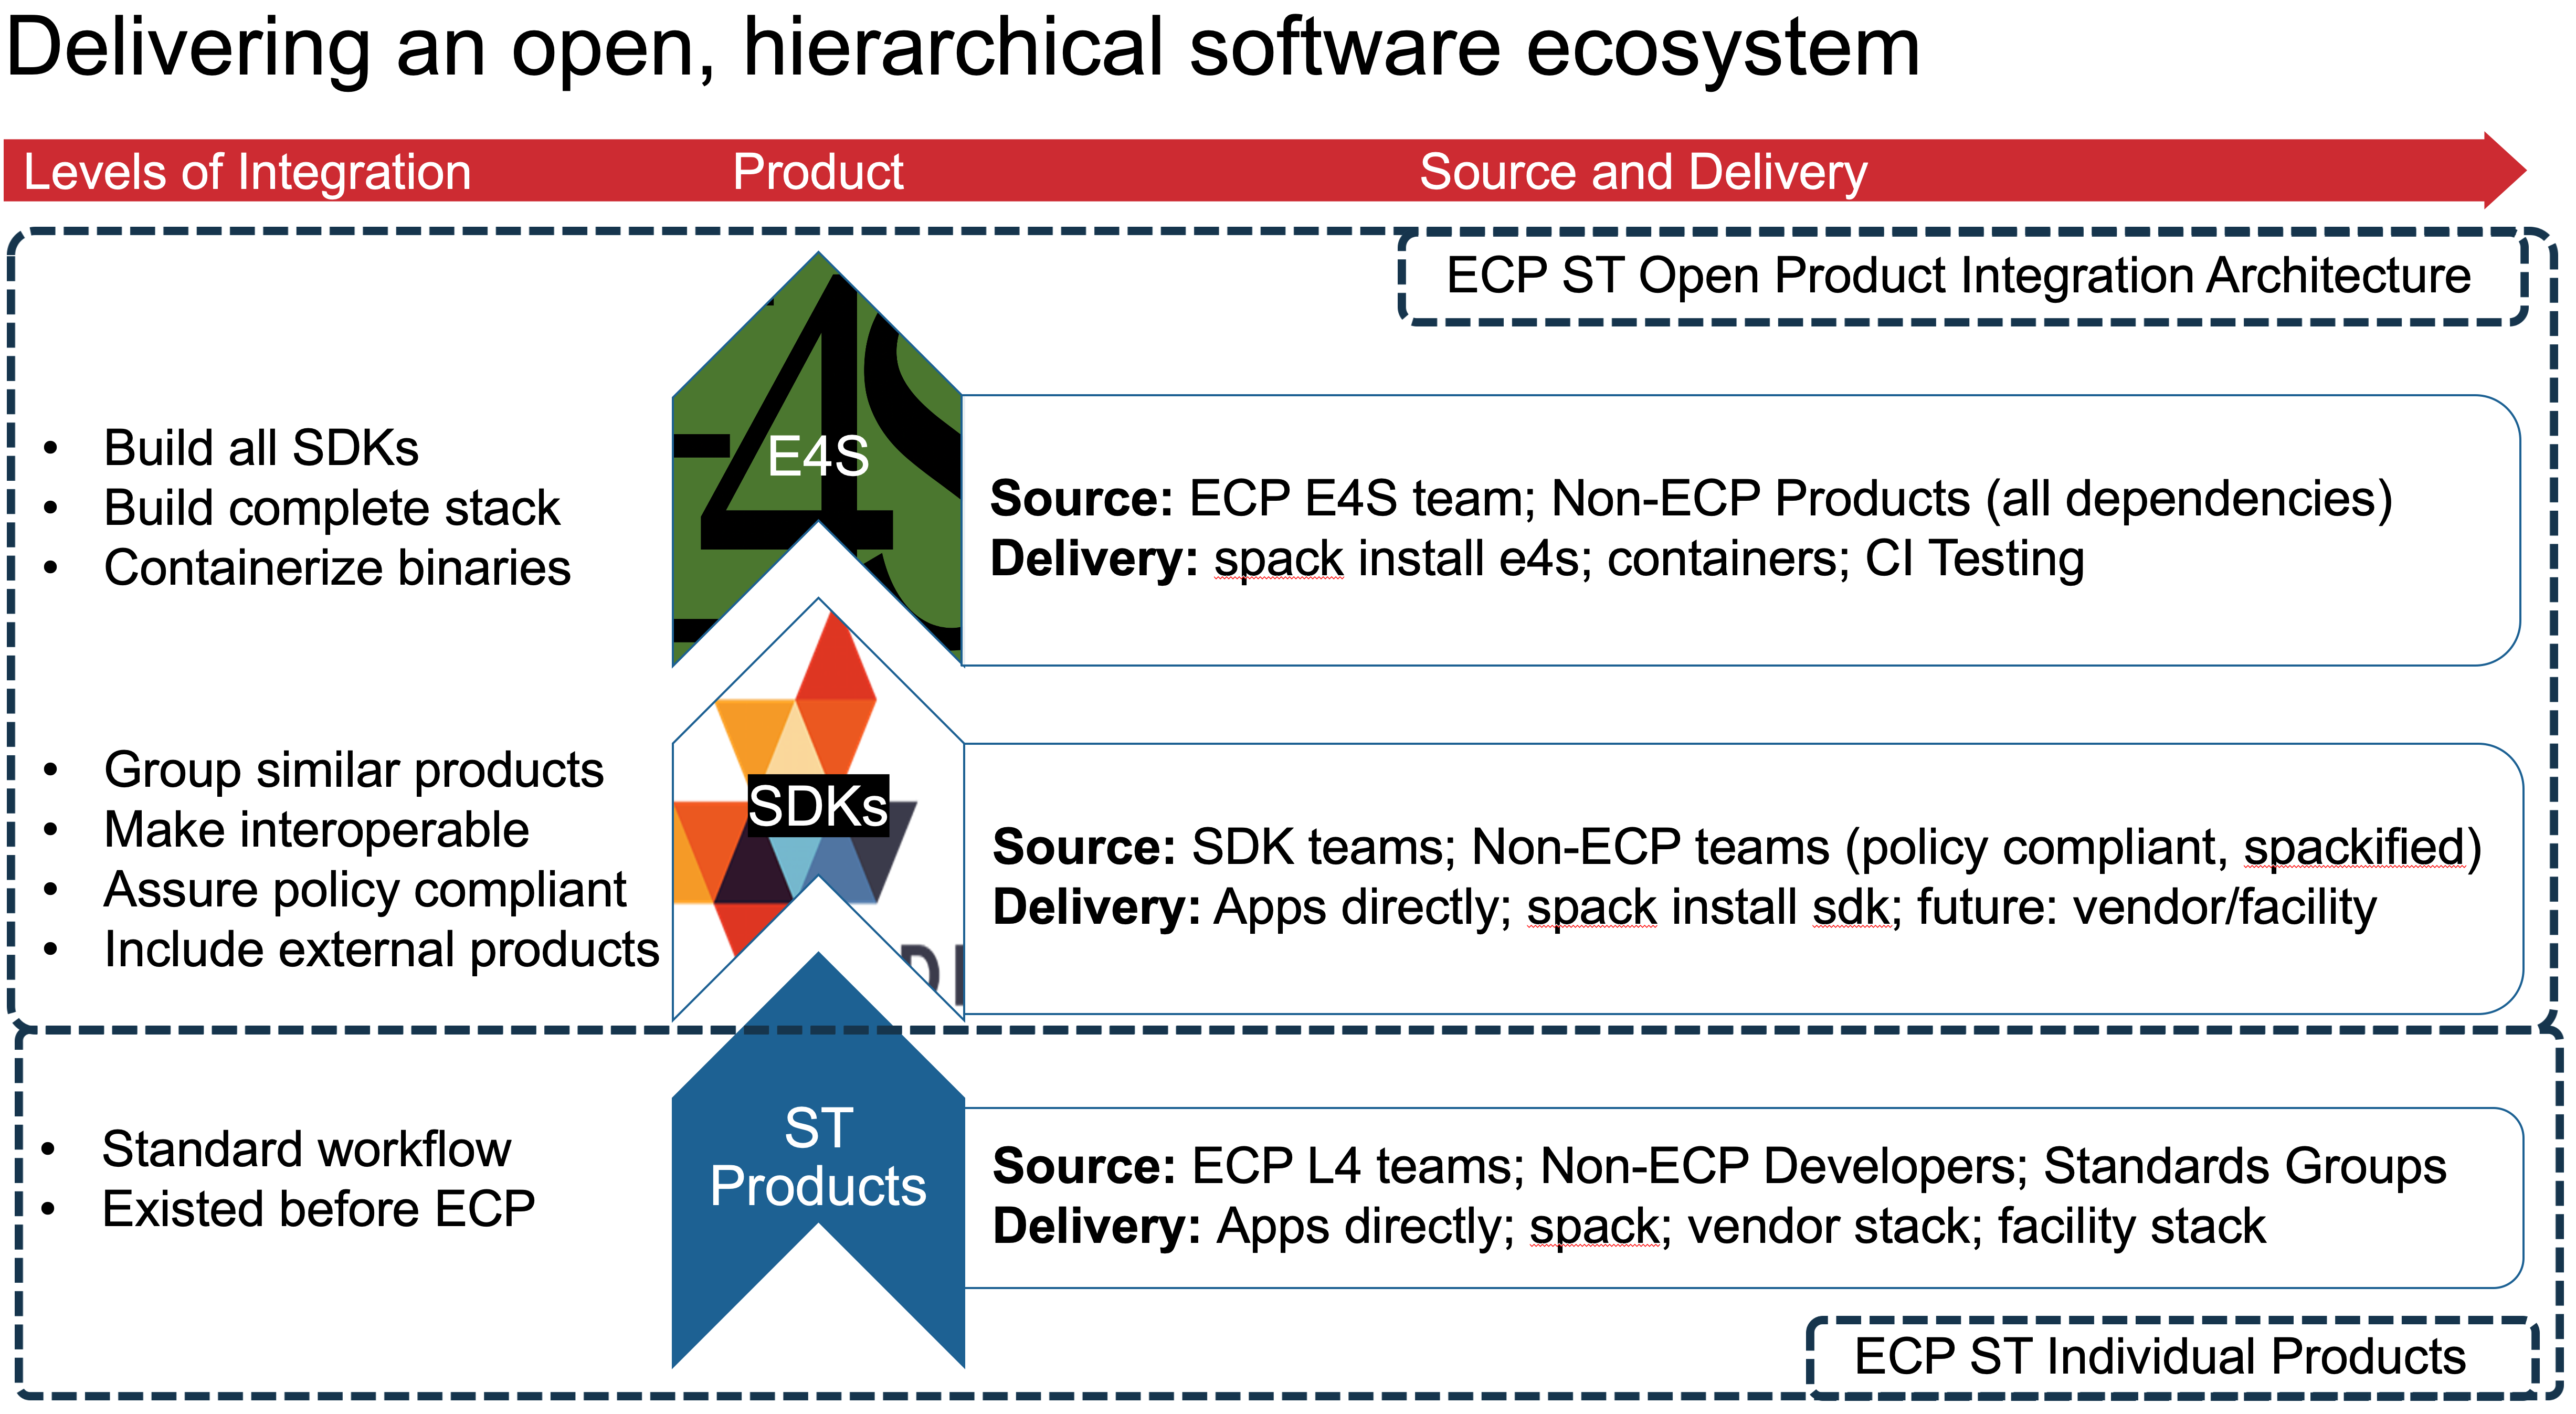
\includegraphics[width=0.9\linewidth]{E4S-Hierarchy}
	\caption{The ECP ST software stack is delivered to the user community through several channels, including via source code, using SDKs, direct to facilities in collaboration with ECP HI, and via binary distributions from containers and HPC vendors.
	Increasingly, E4S is the primary pathway for delivering ECP ST capabilities.  E4S provides testing, a documentation portal, and quality commitments via community policies.}
	\label{fig:hierarchy}
    \protect\todo[inline]{Please replace image with higher resolution image that is not a screenshot so that the image is not blurry and no longer has the red spellcheck underline.}
    \protect\todo[inline]{Capitalize: Spack, SDK, E4S, Spackified.}
\end{figure}

\subsubsection{ECP ST Software Life Cycle}
This section discusses the ECP ST software life cycle, as shown in Figure~\ref{fig:lifecycle}.  From their inception as P6 Activity planning packages, which are refined annually and given detailed information from before starting the activity all the way to the successful integration of a capability into the client environment, ECP ST features are governed by this life cycle.  Each product team conducts its own integration planning that incorporates other funding sources and stakeholders, but the ECP ST life cycle intersects the product life cycle for capabilities that the ECP funds.

\begin{figure}
	\centering
	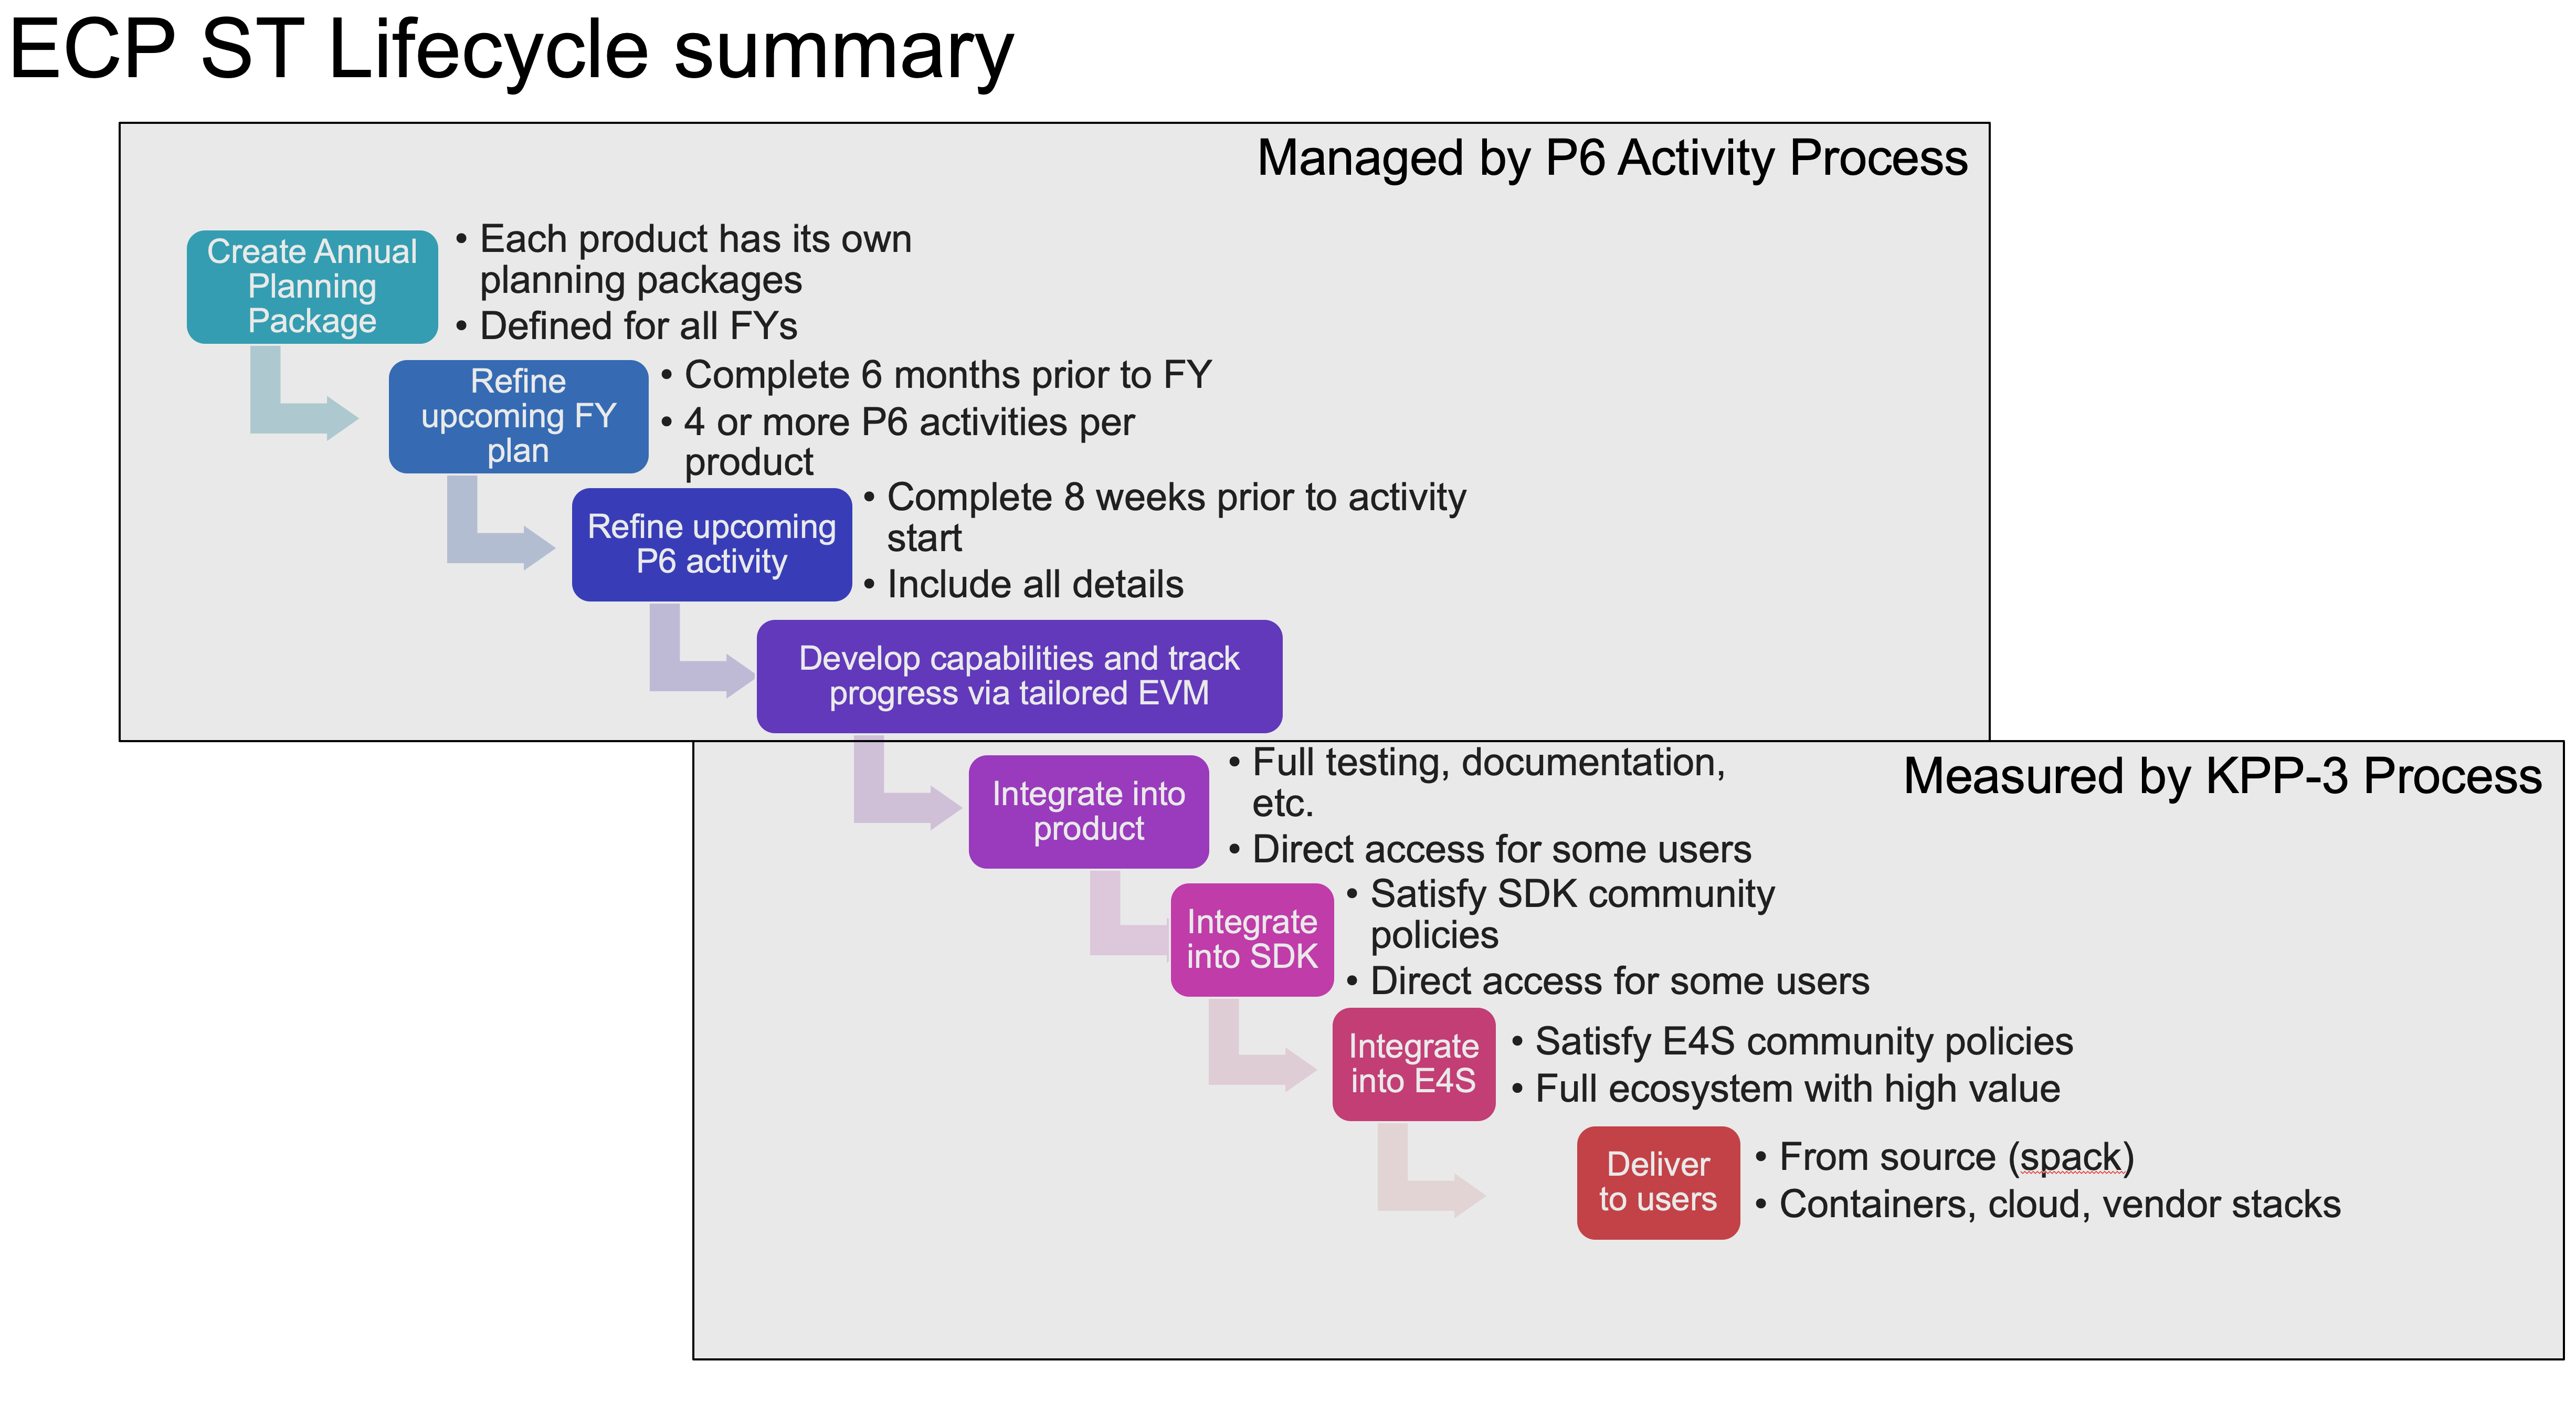
\includegraphics[width=0.9\linewidth]{E4S-Lifecycle}
	\caption{ECP ST product planning, execution, testing, and assessment are governed by the combination of P6 Activities for hierarchical planning (Figure~\ref{fig:planning-process}) and KPP-3 for measuring capability integrations (Table~\ref{table:KPP-3-scoring}).  This figure shows how the entire life cycle of ECP ST feature development is captured by these two elements.}
	\label{fig:lifecycle}
    \protect\todo[inline]{Please replace image with higher resolution image that is not a screenshot so that the image is not blurry and no longer has the red spellcheck underline. Also, if possible to edit image, please change "Lifecycle" to "Life Cycle" (it is two words per Merriam-Webster.)}
    \protect\todo[inline]{Capitalize Spack. Spell out numbers zero through nine.}
\end{figure}



%\newpage
%\section{ECP ST Technical Areas}
%\subsection{\stid{1}  \pmr}\label{subsect:pmr}

\textbf{End State:} A cross-platform, production-ready programming environment that enables and accelerates the development of mission-critical software at both the node and full-system levels.

\subsubsection{Scope and Requirements}
A programming model provides the abstract design upon which developers express and coordinate the efficient parallel execution of their program. A particular model is implemented as a developer-facing interface and a supporting set of runtime layers. To successfully address the challenges of exascale computing, these software capabilities must address the challenges of programming at both the node- and full-system levels. These two targets must be coupled to support multiple complexities expected with exascale systems (e.g., locality for deep memory hierarchies, affinity for threads of execution, load balancing) and also provide a set of mechanisms for performance portability across the range of potential and final system designs. Additionally, there must be mechanisms for the interoperability and composition of multiple implementations (e.g., one at the system level and one at the node level). This must include abilities such as resource sharing for workloads that include coupled applications, supporting libraries and frameworks, and capabilities such as in situ analysis and visualization. 

Given the ECP’s timeline, the development of new programming languages and their supporting infrastructure is infeasible. We do, however, recognize that the augmentation or extension of the features of existing and widely used languages (e.g., C/C++ and Fortran) could provide solutions for simplifying certain software development activities. 

\subsubsection{Assumptions and Feasibility}
The intent of the PMR L3 is to provide a set of programming abstractions and their supporting implementations that allow programmers to select from options that meet demands for expressiveness, performance, productivity, compatibility, and portability. It is important to note that, while these goals are obviously desirable, they must be balanced with an additional awareness that today’s methods and techniques may require changes in both the application and the overall programming environment and within the supporting software stack.

\subsubsection{Objectives}
PMR provides the software infrastructure necessary to enable and accelerate the development of HPC applications that perform well and are correct and robust, while reducing the cost both for initial development and ongoing porting and maintenance. PMR activities need to reflect the requirements of increasingly complex application scenarios, usage models, and workflows, while at the same time addressing the hardware challenges of increased levels of concurrency, data locality, power, and resilience. The software environment will support programming at multiple levels of abstraction that includes both mainstream as well as alternative approaches if feasible in ECP’s timeframe. 

Both of these approaches must provide a portability path such that a single application code can run well on multiple types of systems, or multiple generations of systems, with minimal changes. The layers of the system and programming environment implementation will therefore aim to hide the differences through compilers, runtime systems, messaging standards, shared-memory standards, and programming abstractions designed to help developers map algorithms onto the underlying hardware and schedule data motion and computation with increased automation.
\subsubsection{Plan}
PMR contains nine L4 projects. To ensure relevance to DOE missions, these efforts leverage and collaborate with existing activities within the broader HPC community. The PMR area supports the research and development needed to produce exascale-ready versions of the Message Passing Interface (MPI);  Partitioned Global-Address Space Libraries (UPC++, GASNet); task-based programming models (Legion, PaRSEC); software for node-level performance portability (Kokkos, RAJA); and libraries for memory, power, and resource management.
Initial efforts focused on identifying the core capabilities needed by the selected ECP applications and components of the software stack, identifying shortcomings of current approaches, establishing performance baselines of existing implementations on available petascale and prototype systems, and the re-implementation of the lower-level capabilities of relevant libraries and frameworks. These efforts provided demonstrations of parallel performance of algorithms on pre-exascale, leadership-class machines--at first on test problems, but eventually in actual applications (in close collaboration with the AD and HI teams). Initial efforts also informed research into exascale-specific algorithms and requirements that will be implemented across the software stack. The supported projects targeted and implemented early versions of their software on CORAL, NERSC and ACES pre-exascale systems--with an ultimate target of production-ready deployment on the exascale systems.
In FY20--23, the focus is on development and tuning for the specific architectures of the selected exascale platforms, in addition to tuning specific features that are critical to ECP applications.

Throughout the effort, the applications teams and other elements of the software stack evaluate and provide feedback on their functionality, performance, and robustness. Progress towards these goals is documented quarterly and evaluated annually (or more frequently if needed) based on PMR-centric milestones as well as joint milestone activities shared across associated software stack activities by Application Development and Hardware \& Integration focus areas.


\subsubsection{Risks and Mitigation Strategies}
The mainstream activities of ECP in the area of programming models focus on advancing the capabilities of MPI and OpenMP. Pushing them as far as possible into the exascale era is key to supporting an evolutionary path for applications. This is the primary risk mitigation approach for existing application codes. Extensions to MPI and OpenMP standards require research, and part of the efforts will focus on rolling these findings into existing standards, which takes time. To further address risks, PMR is exploring alternative approaches to mitigate the impact of potential limitations of the MPI and OpenMP programming models. 

Another risk is the failure of adoption of the software stack by the vendors, which is mitigated by the specific delivery focus in sub-element SW Ecosystem and Delivery. Past experience has shown that a combination of laboratory-supported open-source software and vendor-optimized solutions built around standard APIs that encourage innovation across multiple platforms is a viable approach and is what we are doing in PMR. We are using close interaction with the vendors early on to encourage adoption of the software stack, including well-tested practices of including support for key software products or APIs into large procurements through NRE or other contractual obligations. A mitigation strategy for this approach involves building a long-lasting open-source community around projects that are supported via laboratory and university funding. 

Creating a coordinated set of software requires strong management to ensure that duplication of effort is minimized. This is recognized by ECP management, and processes are in place to ensure collaboration is effective, shortcuts are avoided unless necessary, and an agile approach to development is instituted to prevent prototypes moving directly to product. 

\subsubsection{Future Trends}
Recently announced exascale system procurements have shown that the
trend in exascale compute-node hardware is toward heterogeneity:
Compute nodes of future systems will have a combination of regular
CPUs and accelerators (typically GPUs). Furthermore, the GPUs will not
be just from NVIDIA as on existing systems: One system will have Intel
GPUs and another will have AMD GPUs. In other words, there will be a
diversity of GPU architectures, each with their own vendor-preferred
way of programming the GPUs. An additional complication
is that although the HPC community has some experience in using NVIDIA
GPUs and the associated CUDA programming model, the community has relatively
little experience in programming Intel or AMD GPUs.  These
issues lead to challenges for application and software teams in
developing exascale software that is both portable and high performance. Below
we outline trends in programming these complex systems that will help
alleviate some of these challenges.

\paragraph{Trends in Internode Programming}
The presence of accelerator hardware on compute nodes has resulted in individual
compute nodes becoming very powerful. As a result, millions of compute
nodes are no longer needed to build an exascale system. This trend
results in a lower burden on the programming system used for internode
communication. It is widely expected that MPI will continue to serve
the purpose of internode communication on exascale systems and is the
least disruptive path for applications, most of which already use
MPI. Nonetheless, improvements are needed in the MPI Standard as well
as in MPI implementations in areas such as hybrid programming
(integration with GPUs and GPU memory, integration with the intranode
programming model), overall resilience and robustness, scalability,
low-latency communication, optimized collective algorithms, optimized support
for exascale interconnects and lower-level communication paradigms
such as OFI and UCX, and scalable process startup and management. PGAS
models, such as UPC++ and OpenSHMEM, are also available to be used by
applications that rely on them and face similar
challenges as MPI on exascale systems. These challenges are being tackled by the MPI and
UPC++/GASNet projects in the PMR area.

\paragraph{Trends in Intranode Programming}
The main challenge for exascale is in achieving performance and portability for
intranode programming, for which a variety of options
exist. Vendor-supported options include CUDA and OpenACC for NVIDIA
GPUs, SYCL/DPC++ for Intel GPUs, and HIP for AMD GPUs. OpenACC
supports accelerator programming via compiler directives. SYCL
provides a C++ abstraction on top of OpenCL, which itself is a
portable, lower-level API for programming heterogeneous
devices. Intel's DPC++ is similar to SYCL with some extensions. HIP
from AMD is similar to CUDA; in fact, AMD provides translation tools
to convert CUDA programs to HIP.

Among portable, standard programming models, OpenMP has supported
accelerators via the \texttt{target} directive starting with OpenMP version
4.0 released in July 2013. Subsequent releases of OpenMP (version 4.5
and 5.0) have further improved support for accelerators. OpenMP is
supported by vendors on all platforms and, in theory, could serve as a
portable intranode programming model for systems with
accelerators. However, in practice, a lot depends on the quality of
the implementation.

Kokkos and RAJA provide another alternative for portable,
heterogenous-node programming via C++ abstractions. They
are designed to work on complex node architectures
with multiple types of execution resources and multilevel memory
hierarchies. Many ECP applications are successfully using Kokkos and
RAJA to write portable parallel code that runs efficiently on GPUs.

We believe these options (and high-quality implementations of them) will
meet the needs of applications in the exascale timeframe. 

%\subsection{\stid{2} \tools}\label{subsect:tools}

\textbf{End State:}	A suite of compilers and development tools aimed at improving developer productivity across increasingly complex heterogeneous architectures, primarily focused on those architectures expected for the upcoming Exascale platforms of Frontier and Aurora.

\subsubsection{Scope and Requirements}

For Exascale systems, the compilers, profilers, debuggers, and other software development tools must be increasingly sophisticated to give software developers insight into the behavior of not only the application and the underlying hardware but also the details corresponding to the underlying programming model implementation and supporting runtimes (e.g., capturing details of locality and affinity). These capabilities should be enhanced with further integration into the supporting compiler infrastructure and lower layers of the system software stack (e.g., threading, runtime systems, and data transport libraries), and hardware support. Most of the infrastructure will be released as open source, as many of them already are, with a supplementary goal of transferring the technology into commercial products (including reuse by vendors of ECP enhancements to LLVM, such as Fortran/Flang, or direct distributions by vendors of software on platforms). Given the diversity of Exascale systems architectures, some subset of the tools may be specific to one or more architectural features and is potentially best implemented and supported by the vendor; however, the vendor will be encouraged to use open APIs to provide portability, additional innovation, and integration into the tool suite and the overall software stack.

\subsubsection{Assumptions and Feasibility }

The overarching goal of improving developer productivity for Exascale platforms introduces new issues of scale that will require more lightweight methods, hierarchical approaches, and improved techniques to guide the developer in understanding the characteristics of their applications and to discover sources of the errors and performance issues. Additional efforts for both static and dynamic analysis tools to help identify lurking bugs in a program, such as race conditions, are also likely needed. The suite of needed capabilities spans interfaces to hardware-centric resources (e.g., hardware counters, interconnects, and memory hierarchies) to a scalable infrastructure that can collect, organize, and distill data to help identify performance bottlenecks and transform them into an actionable set of steps and information for the software developer. Therefore, these tools share significant challenges due to the increase in data and the resulting issues with management, storage, selection, analysis, and interactive data exploration. This increased data volume stems from multiple sources, including increased concurrency, processor counts, additional hardware sensors and counters on the systems, and increasing complexity in application codes and workflows.

Compilers obviously play a fundamental role in the overall programming environment but can also serve as a powerful entry point for the overall tool infrastructure. In addition to optimizations and performance profiling, compiler-based tools can help with aspects of correctness, establishing connections between programming model implementations and the underlying runtime infrastructures, and auto-tuning. In many cases, today's compiler infrastructure is proprietary and closed source, limiting the amount of flexibility for integration and exploration into the Exascale development environment. In addition to vendor compiler options, this project aims to provide an open source compiler capability (via the LLVM ecosystem) that can play a role in better supporting and addressing the challenges of programming at Exascale. 


\subsubsection{Objectives}

This project will design, develop, and deploy an Exascale suite of compilers and development tools for development, analysis, and optimization of applications, libraries, and infrastructure from the programming environments of the project.  
The project will seek to leverage techniques for common and identified problem patterns and create new techniques for data exploration related to profiling and debugging and support advanced techniques such as autotuning and compiler integration. 
We will leverage the open-source LLVM compiler ecosystem. 
For tools, the overarching goal is to leverage and integrate the data measurement, acquisition, storage, and analysis and visualization techniques being developed in other projects of the software stack.  
These efforts will require collaboration and integration with system monitoring and various layers within the software stack.


\subsubsection{Plan}
Multiple projects will be supported under this effort. To ensure relevance to DOE missions, a majority of these efforts shall be DOE laboratory led, and collaborate with existing activities within the broader HPC community. 
Initial efforts will focus on identifying the core capabilities needed by the selected ECP applications, components of the software stack, expected hardware features, and the selected industry activities from within the Hardware and Integration focus area. 
The supported projects will target and implement early versions of their software on both CORAL and APEX systems, with an ultimate target of production-ready deployment on Frontier and Aurora. 
Throughout this effort the, applications teams and other elements of the software stack will evaluate and provide feedback on their functionality, performance, and robustness. 
These goals will be evaluated annually at the ST reviews and for milestones.

\subsubsection{Risk and Mitigation Strategies}

A primary risk exists in terms of adoption of the various tools by the broader community, including support by system vendors. Past experience has shown that a combination of laboratory-supported open source software and vendor-optimized solutions built around standard APIs that encourage innovation across multiple platforms is a viable approach, and this will be undertaken. 
We will track this risk primarily via the risk register.

Given its wide use within a range of different communities, and its modular design principles, the project's open source compiler activities will focus on the use of the LLVM compiler ecosystem (\url{https://llvm.org/}) as a path to reduce both scope and complexity risks and leverage with an already established path for NRE investments across multiple vendors. 
The compilers and their effectiveness are tracked in the risk register. 
%
In fact, in 2020, we created a fork of the llvm-project upstream repository (see \url{https://github.com/llvm-doe-org}) to capture, integrate, and test LLVM projects. This repo also serves as a risk mitigation option that can be easily enabled if other compilers are not working successfully on the target platforms.

Another major risk for projects in this area is the lack of low-level access to hardware and software necessary for using emerging architectural features. Many of these nascent architectural features have immature implementations and software interfaces that must be refined prior to release to the broader community. This project should be at the forefront of this interaction with early delivery systems. This risk is also tracked in the risk register for compilers, which are particularly vulnerable.

\subsubsection{Future Trends}

Future architectures are becoming more heterogeneous and complex~\cite{vetter:2018:extreme}. As such, the role of languages, compilers, runtime systems, and performance and debugging tools will becoming increasingly important for productivity and performance portability. 
%
In particular, our ECP strategy focuses on improving the open source LLVM compiler and runtime ecosystem; LLVM has gained considerable traction in the vendor software community, and it is the core of many existing heterogeneous compiler systems from NVIDIA, AMD, Intel, ARM, IBM, and others. 
Over the past two years, several vendors including IBM and Intel have abandoned their proprietary compiler software in favor of LLVM. 
We foresee that this trend will continue, which is why we have organized the \tools\ technical area around LLVM-oriented projects.  
%
We expect for many of our contributions to LLVM to address these trends for the entire community and will persist long after ECP ends. 
%
For example, our contributions for directive-based features for heterogeneous computing (e.g., OpenMP, OpenACC) will not only provide direct capabilities to ECP applications, but it will also impact the redesign and optimization of the LLVM infrastructure to support heterogeneous computing.
%
In a second example, Flang (open source Fortran compiler for LLVM; [the second version is also known as F18]) will become increasingly important to the worldwide Fortran application base, as vendors find it easier to maintain and deploy to their own Fortran frontend (based on Flang).  
%
Furthermore, as Flang become increasingly robust, researchers and vendors developing new architectures will have immediate access to Flang, making initial Fortran support straightforward in ways similar to what we are seeing in Clang as the community C/C++ frontend.

%

%\subsection{\stid{3} \mathlibs}\label{subsect:mathlibs}

\textbf{End State:} Mathematical libraries that (i) interoperate with the ECP software stack; (ii) are incorporated into the ECP applications; and (iii) provide scalable, resilient numerical algorithms that facilitate efficient simulations on Exascale computers.

\subsubsection{Scope and Requirements}
Software libraries are powerful means of sharing verified, optimized algorithms and their implementations. Applied research, development, and support are needed to extend existing DOE mathematical software libraries to make better use of Exascale architectural features. DOE-supported libraries encapsulate the latest results from mathematics and computer science R\&D; many DOE mission-critical applications rely on these numerical libraries and frameworks to incorporate the most advanced technologies available. 

The Mathematical Libraries effort will ensure the healthy functionality of the numerical software libraries on which the ECP applications will depend. The DOE mathematical software libraries used by computational science and engineering applications span the range from light-weight collections of subroutines with simple APIs to more “end-to-end” integrated environments and provide access to a wide range of algorithms for complex problems.

Advances in mathematical and scientific libraries will be necessary to enable computational science on Exascale systems. Exascale computing promises not only to provide more computational resources enabling higher-fidelity simulations and more demanding studies but also to enable the community to pose new scientific questions. Exascale architectural characteristics introduce new features that algorithms and their implementations will need to address in order to be scalable, efficient, and robust. As a result, it will be necessary to conduct research and development to rethink, reformulate, and develop existing and new methods and deploy them in libraries that can be used by applications to deliver more complete and sophisticated models and provide enhanced predictive simulation and analysis capabilities.

The Mathematical Libraries effort must (1) collaborate closely with the Application Development effort (WBS 2.2) to be responsive to the needs of the applications and (2) collaborate with the other products within the Software Technology effort (WBS 2.3) in order to incorporate new technologies and to provide requirements. All software developed within the Mathematical Libraries effort must conform to best practices in software engineering, which will be formulated early in the project in collaboration with the Applications Development focus area. Software produced by this effort must provide scalable numerical algorithms that enable the application efforts to reach their performance goals, encapsulated in libraries whose data structures and routines can be used to build application software.

\subsubsection{Assumptions and Feasibility}
Years of DOE investment have led to a diverse and complementary collection of mathematical software, including AMReX, Chombo, hypre, Dakota, DTK, MAGMA, MFEM, PETSc/TAO, PLASMA, ScaLAPACK, SUNDIALS, SuperLU, and Trilinos. This effort is evolving a subset of existing libraries to be performant on Exascale architectures. In addition, research and development is needed into new algorithms whose benefits may be seen only at the extreme scale. Results of preliminary R\&D projects indicate that this approach is feasible.

Additionally, ECP will need to rely on a strong, diverse, and persistent base math research program, which is assumed to continue being supported by the DOE-SC ASCR Office. The ECP technical directors will schedule quarterly meetings with the ASCR research program managers to get updates on research results that might meet ECP requirements as well as to inform the program managers of ECP needs in applications and software components.

\subsubsection{Objectives}
The high-level objective of the Mathematical Libraries effort is to provide scalable, resilient numerical algorithms that facilitate efficient application simulations on Exascale computers. To the greatest extent possible, this objective should be accomplished by preserving the existing capabilities in mathematical software while evolving the implementations to run effectively on the Exascale systems and adding new capabilities that may be needed by Exascale applications.

The key performance metrics for the software developed by this effort are scalability, efficiency, and resilience. As a result of the new capabilities in mathematics libraries developed under this effort, applications will tackle problems that were previously intractable and will model phenomena in physical regimes that were previously unreachable.

\subsubsection{Plan}
As detailed below, the Mathematical Libraries effort supports six complementary L4 projects as needed to meet the needs of ECP applications. These efforts include strong collaborations among DOE labs, academia, industry, and other organizations, and leveraging existing libraries that are widely used by the DOE HPC community. 

Initial efforts have focused on identifying core capabilities needed by selected ECP applications, establishing performance baselines of existing implementations on available Petascale and prototype systems, and beginning re-implementation of lower-level capabilities of the libraries and frameworks. Another key activity is collaborating across all projects in the Mathematical Libraries effort to define community policies in order to enable compatibility among complementary software and to provide a foundation for future work on deeper levels of interoperability. Refactoring of higher-level capabilities will be prioritized based on needs of the applications. In time, these efforts will provide demonstrations of parallel performance of algorithms from the mathematical software on pre-Exascale, leadership-class machines (at first on test problems, but eventually in actual applications). The initial efforts also are informing research into advanced exascale-specific numerical algorithms that will be implemented within the libraries and frameworks. In FY20–23, the focus will be on development and tuning for the specific architectures of the selected exascale platforms, in addition to tuning specific features that are critical to ECP applications. The projects will implement their software on the CORAL, NERSC and ACES systems,
the pre-Exascale hardwares such as Tulip and Iris,
and ultimately on initial Exascale systems, so that functionality, performance, and robustness can be evaluated by the applications teams and other elements of the software stack. Throughout the effort the applications teams and other elements of the software stack will evaluate and provide feedback on their functionality, performance, and robustness. These goals will be evaluated at least yearly based on milestones as well as joint milestone activities shared across the associated software stack activities by Application Development and Hardware and Integration project focus areas.


\subsubsection{Risks and Mitigations Strategies}
There are a number of foreseeable risks associated with the Mathematical Libraries effort.
\begin{itemize}
\item Efficient implementation of new or refactored algorithms to meet Exascale computing requirements may introduce unanticipated requirements on programming environments. To mitigate this risk, effective communication is needed between projects in the Mathematical Libraries effort and projects tasked with developing the programming environments. From the application perspective, this is specifically tracked in a specific AD risk
  in the risk register. Additionally, the risks of an inadequate programming environment overall are tracked as a specific ST risk in the risk register.
	\item A significant number of existing algorithms currently implemented in numerical libraries may scale poorly, thereby requiring significantly more effort than refactoring. The R\&D planned for the first three years of the ECP is the first mitigation for this risk (as well as the co-design centers planned in Application Development). In addition, the ECP will be able to draw from a strong, diverse, well-run, persistent base math research program. From the application perspective, this is tracked via an AD risk in the risk register. Scaling issues for the software stack in general, including libraries, are monitored via an ST risk in the risk register.
	\item Exascale architecture characteristics may force a much tighter coupling among the models, discretizations, and solvers employed, causing general-purpose solvers to be too inefficient. The mitigation strategy is to ensure close collaboration with the sub-elements of the Application Development focus area (WBS 2.2) to understand integration and coupling issues. Again, a strong, diverse, well-run, persistent base math research program may provide risk mitigation strategies.
\end{itemize}

\subsubsection{Future Trends}
Mathematical libraries have been one of the strongest success stories in the scientific software ecosystem.  These libraries encode specialized algorithms on advanced computers that can be the difference between success or not.  Algorithms such as multigrid, highly-tuned dense linear algebra and optimized FFTs, can improve performance by orders of magnitude and reduce the asymptotic algorithmic complexity for users.  We foresee that math libraries will have an ever-growing role in the scientific software ecosystem, as architectures become more challenging for targeting optimization and algorithms require even more concurrency and latency hiding in order to realize performance on modern computer systems.

In addition, we anticipate that new algorithms based on multi-precision arithmetic will further enable performance improvements on compute devices that are optimized for machine learning workloads,
where lower precision can be an order of magnitude faster that double precision.
A recent paper~\cite{Anztetal2020} surveys the landscape of multi-precision numerical
linear algebra algorithms.

For a deeper discussion of the futures of ECP Math Libraries efforts, please consult the paper ``Preparing Sparse Solvers for Exascale Computing''~\cite{ECP-Solvers}.

%\subsection{\stid{4} \dataviz}\label{subsect:dataviz}

\textbf{End State:} A production-quality storage infrastructure necessary to manage, share, and facilitate analysis of data in support of mission critical codes. Data analytics and visualization software that effectively supports scientific discovery and understanding of data produced by Exascale platforms.

\subsubsection{Scope and Requirements}
Changes in the hardware architecture of Exascale supercomputers will render current approaches to data management, analysis and visualization obsolete, resulting in disruptive changes to the scientific workflow and rendering traditional checkpoint/restart methods infeasible. A major concern is that Exascale system concurrency is expected to grow by five or six orders of magnitude, yet system memory and input/output (I/O) bandwidth/persistent capacity are only expected to grow by one and two orders of magnitude, respectively. The reduced memory footprint per FLOP further complicates these problems, as does the move to a hierarchical memory structure. Scientific workflow currently depends on exporting simulation data off the supercomputer to persistent storage for post-hoc analysis.

On Exascale systems, the power cost of data movement and the worsening I/O bottleneck will make it necessary for most simulation data to be analyzed in situ, or on the supercomputer while the simulation is running. Furthermore, to meet power consumption and data bandwidth constraints, it will be necessary to sharply reduce the volume of data moved on the machine and especially the data that are exported to persistent storage. The combination of sharp data reduction and new analysis approaches heighten the importance of capturing data provenance (i.e., the record of what has been done to data) to support validation of results and post-hoc data analysis and visualization.
Data and Visualization is the title for Data Management (DM) \& Data Analytics and Visualization (DAV) activities in the Exascale project.

Data management (DM) activities address the severe I/O bottleneck and challenges of data movement by providing and improving storage system software; workflow support including provenance capture; and methods of data collection, reduction, organization and discovery.

Data analytics and visualization (DAV) are capabilities that enable scientific knowledge discovery. Data analytics refers to the process of transforming data into an information-rich form via mathematical or computational algorithms to promote better understanding. Visualization refers to the process of transforming scientific simulation and experimental data into images to facilitate visual understanding. Data analytics and visualization have broad scope as an integral part of scientific simulations and experiments; they are also a distinct separate service for scientific discovery, presentation and documentation purposes, as well as other uses like code debugging, performance analysis, and optimization. 

The scope of activities falls into the following categories:
\begin{itemize}
\item Scalable storage software infrastructure – system software responsible for reliable storage and retrieval of data supporting checkpointing, data generation, and data analysis I/O workloads
\item Workflow and provenance infrastructure – facilitating execution of complex computational science processes and the capture and management of information necessary to interpret and reproduce results
\item Data collection, reduction, and transformation – enabling complex transformation and analysis of scientific data where it resides in the system and as part of data movement, in order to reduce the cost to solution
\item Data organization and discovery – indexing and reorganizing data so that relevant items can be identified in a time- and power-efficient manner, and complex scientific data analysis can be performed efficiently on Exascale datasets
\item In situ algorithms and infrastructure – performing DAV while data is still resident in memory as the simulation runs enabling automatic identification, selection and data reduction for Exascale applications.
\item Interactive post-hoc approaches – on data extracts that produced in situ and support post-hoc understanding through exploration.
\item Distributed memory multi-core and many-core approaches, for the portable, performant DM and DAV at Exascale.
\end{itemize}
\subsubsection{Assumptions and Feasibility}
\begin{itemize}
\item Scaling up traditional DM and DAV approaches is not a viable approach due to severe constraints on available memory and I/O capacity, as well as dramatically different processor and system architectures being at odds with contemporary DAV architectures.
\item Simulations will produce data that is larger and more complex, reflecting advances in the underlying physics and mathematical models. Science workflows will remain complex, and increasing requirements for repeatability of experiments, availability of data, and the need to find relevant data in Exascale datasets will merit advances in workflow and provenance capture and storage.
\item The expense of data movement (in time, energy, and dollars) will require data reduction methods, shipping functions to data, and placing functionality where data will ultimately reside.
\item Solid-state storage will become cheaper, denser, more reliable, and more ubiquitous (but not cheap enough to replace disk technology in the Exascale timeframe). Exascale compute environments will have in-system nonvolatile storage and off-system nonvolatile storage in addition to disk storage. Applications will need help to make use of the complex memory/storage architectures.
\item Disks will continue to gain density but not significant bandwidth; disks will become more of a capacity solution and even less a bandwidth one.
\item Industry will provide parts of the overall data management, data analysis and visualization solution, but not all of it; non-commercial parts will be produced and maintained.
\item This plan and associated costs were formulated based on the past decade of DOE visualization and data analysis activities, including the successful joint industry/laboratory-based development of open-source visualization libraries and packages (VTK, VisIt, and ParaView).
\end{itemize}
\subsubsection{Objectives}
Data management, analysis and visualization software must provide:
\begin{itemize}
\item production-grade Exascale storage infrastructure(s), from application interfaces to low-level storage organization, meeting requirements for performance, resilience, and management of complex Exascale storage hierarchies;
\item targeted research to develop a production-grade in situ workflow execution system, to be integrated with vendor resource management systems, meeting science team requirements for user-defined and system-provided provenance capture and retention;
\item production-grade system-wide data transfer and reduction algorithms and infrastructure, with user interface and infrastructure for moving/reducing data within the system, to be integrated with vendor system services and meeting science and national security team requirements; and
\item production-grade metadata management enabling application and system metadata capture, indexing, identification, and retrieval of subsets of data based on complex search criteria and ensures that technologies target science and national security team requirements.
\item targeted research to develop a production-grade in situ algorithms, to be integrated with open source visualization and analysis tools and infrastructure, meeting science team data reduction requirements
\item targeted research to develop a production-grade algorithms for the new types of data that will be generated and analyzed on Exascale platforms as a result of increased resolution, evolving scientific models and goals, and increased model and data complexity.
\item targeted research to develop a production-grade post-hoc approach that support interactive exploration and understanding of data extracts produced by in situ algorithms
\item production-grade Exascale data analysis and visualization algorithms and infrastructure, meeting requirements for performance, portability and sustainability for evolving hardware architectures and software environments. 
\end{itemize}

\subsubsection{Plan}
Particularly in the area of DM, productization of technologies is a necessary step for adoption, research-quality software is not enough. One approach we will take is to fund vendors of products in related areas to integrate specific technologies into their product line. When developing objectives for this activity, a focus was placed on the availability of products that deliver these technologies on platforms of interest. Activities can be separated into two categories:
\begin{itemize}
\item Community/Coordination – designed to build the R\&D community, inform ourselves and the community regarding activities in the area, track progress, and facilitate coordination.
\item Targeted R\&D – filling gaps in critical technology areas (storage infrastructure, workflow, provenance, data reduction and transformation, and organization and discovery).
\end{itemize}
In the workflows area, the first 3 years of the project will identify existing software systems that are in use by the DOE community and are aimed at applications that require HPC systems (eventually Exascale systems) and support further R\&D to the emerging requirements of Exascale workflows as well as interaction with other parts of the software stack and adaptation to Exascale hardware architectures.

Portions of the DAV software stack are being productized and supported by industry, which will help to control costs in the long term. Activities to achieve the DAV objectives are heavily dependent on developments across the Exascale project, and thus close coordination with other teams is essential. Close engagement with application scientists is crucial to the success of DAV, both in terms of understanding and addressing the requirements of science at scale and ensuring that computational scientists are able to adopt and benefit from the DAV deliverables.

Many objectives need initial research projects to define plausible solutions. These solutions will be evaluated and progressively winnowed to select the best approaches for the Exascale machine and the needs of science. Selected projects will continue to receive support to extend their research and development efforts to integrate their solutions into the open-source Exascale software stack. 

\subsubsection{Risks and Mitigations Strategies}
There are specific risks identified for the Data and Visualization portfolio.  These risks are tracked in the risk register .  
\begin{itemize}
\item Application teams may continue to employ ad hoc methods for performing data management in their work, resulting in increased I/O bottlenecks and power costs for data movement. Application team engagement, working within the overall software stack, and input into Hardware Integration will be necessary if results are to be deployed, adopted, and significantly improve productivity.
\item Despite funding vendor activities, industry partners may determine the market is insufficient to warrant meeting Exascale requirements.
\item If vendor integration and targeted R\&D activities are not closely coordinated, gaps will not be effectively identified and targeted, or successful R\&D will not be integrated into industry products in the necessary timeframe.
\item Vendors supplying data management solutions are likely to be distinct from Exascale system vendors. Additional coordination will be necessary, beyond DM productization, in order to ensure interoperability of DM solutions with specific Exascale platforms.
\item Data management from an application perspective is tracked in one of the identified risks.  Additionally, the software stack tracks several risks indirectly related to data management as well.
\item Failure of scientists to adopt the new DAV software is a major risk that is exacerbated if the DAV software is research quality. Mitigating this risk depends on close engagement with domain scientists and supporting layers of the software stack through co-design activities, as well as investment in development and productization of DAV codes.
\item Redundant efforts in domain science communities and within ASCR-supported activities such as SciDAC result in wasted resources. Communication and close coordination provide the best strategy for mitigation.
\item Fierce industry and government competition for DAV experts creates a drain on laboratory personnel in DAV and makes lab hiring in this area difficult. Stable funding and a workforce development program would help to mitigate these risks.
\item A skilled workforce is required for a successful Exascale project.
\end{itemize}

\subsubsection{Future Trends}

\textbf{Graphics Architectures and Approaches}  Graphics architectures are improving in terms of raw computational power and through the addition of specialized libraries for accelerating ray-tracing, volume rendering, and denoising. Nvidia has added specialized hardware processing units for ray-tracing and machine learning to their GPU offerings.  Intel has developed a suite of CPU accelerated libraries that support OpenGL (OpenSWR), ray-tracing (Embree, OSPRay), volume rendering (Open Volume Kernel Library) and de-noising (Open Image Denoise). From a visualization and rendering perspective, ray-tracing provides significantly improved rendered results over traditional scan-conversion based approaches.  A near-term opportunity is to take advantages of such functionality for our rendering needs. Longer term, we will look into leveraging these hardware accelerated approaches to accelerate visualization and analysis tasks.

\textbf{In Situ Analysis and Automation}  A key thrust of the Data and Visualization area is the focus on in situ analysis in order to filter important information as it is being generated by the simulations. In addition to our algorithmic and infrastructure efforts, automatic techniques and workflows must be developed to guide the overall in situ analysis process.

\textbf{Workflows} Slowly, more complex workflows are becoming a more significant component of the job mix on ECP-relevant platforms, partially driven by the increased use of these systems for machine learning applications. Workflows can drive degenerate use cases in the storage stack, such as the use of the file system for communication between tasks, when tools from outside the HPC community are adopted without change. Alternative approaches to enable communication between tasks exist but must be adapted to facility contexts, and technical roadblocks (e.g., difficulty in communicating between separate jobs) must be overcome.

\textbf{AI} AI applications will appear more frequently in the job mix. This impacts the requirements for data storage, as new classes of data become more prominent in application input datasets. It also impacts technologies for understanding application behavior, as these jobs are often not using MPI, a common assumption in tool sets. Finally AI-focused applications do not exhibit the common pattern of alternating phases of I/O and computation seen in simulation codes, driving a need for attention on methods of I/O optimization that do not rely on explicit collective I/O phases.

\textbf{Networks} Network architectures are still in flux, and specific new technologies such as Slingshot from Cray will bring new capabilities such as more advanced congestion detection and mitigation that change how networks will behave in the face of mixed communication and I/O traffic or the impact of communication-heavy applications on other applications in the system, etc.  Assumptions regarding how I/O traffic fits into this picture may need to be reexamined. The libfabric interface for accessing networks appears to be the most promising portable interface for use outside of MPI, and teams will need to assess how to best use libfabric across platforms of interest as well as possibly advocating for specific capabilities in libfabric that fall outside of traditional MPI use cases, such as the common pattern of clients connecting and detaching from long-running services.

\textbf{Object stores} Facilities are planning deployments of non-POSIX storage solutions. One of the first of these will be the DAOS deployment on the A21 system at Argonne. The DAOS interfaces are available for teams to begin to understand, an HDF5 front-end for DAOS is available, and there are some examples of DAOS use for scientific codes. It is likely that the highest performance will come from applications directly using the DAOS APIs, and work to allow understanding of how these APIs are used would be beneficial.

\textbf{Compression} Compression will continue to play an important role in computation as a vehicle for addressing the explosion in size of datasets and outputs. Improved integration of compression capabilities in libraries supporting parallel I/O will continue to be a topic for further development, and techniques for allowing concurrent updates while compression is enabled specifically need more exploration.  The use of lower precision data types has the potential of speeding up the visualization and analysis process as well as reducing data sizes without significantly degrading the accuracy of results. 

\textbf{Storage technologies and architectures} Even in systems that will continue to employ POSIX file systems as the main "scratch" store, the hardware on which these file systems are stored will be changing. For example, the Perlmutter system will provide a 30~PB nonvolatile storage tier using Lustre. The file system teams (e.g., Lustre team) will be working to maximize performance on these new storage back-ends, but simultaneously higher software layers must consider how this significant change impacts their assumptions about the relative costs of communication and data storage for common patterns of access.


% STORAGE ARCH. DIAGRAM -- HIGH LEVEL
\begin{figure}[t]
	\centering
	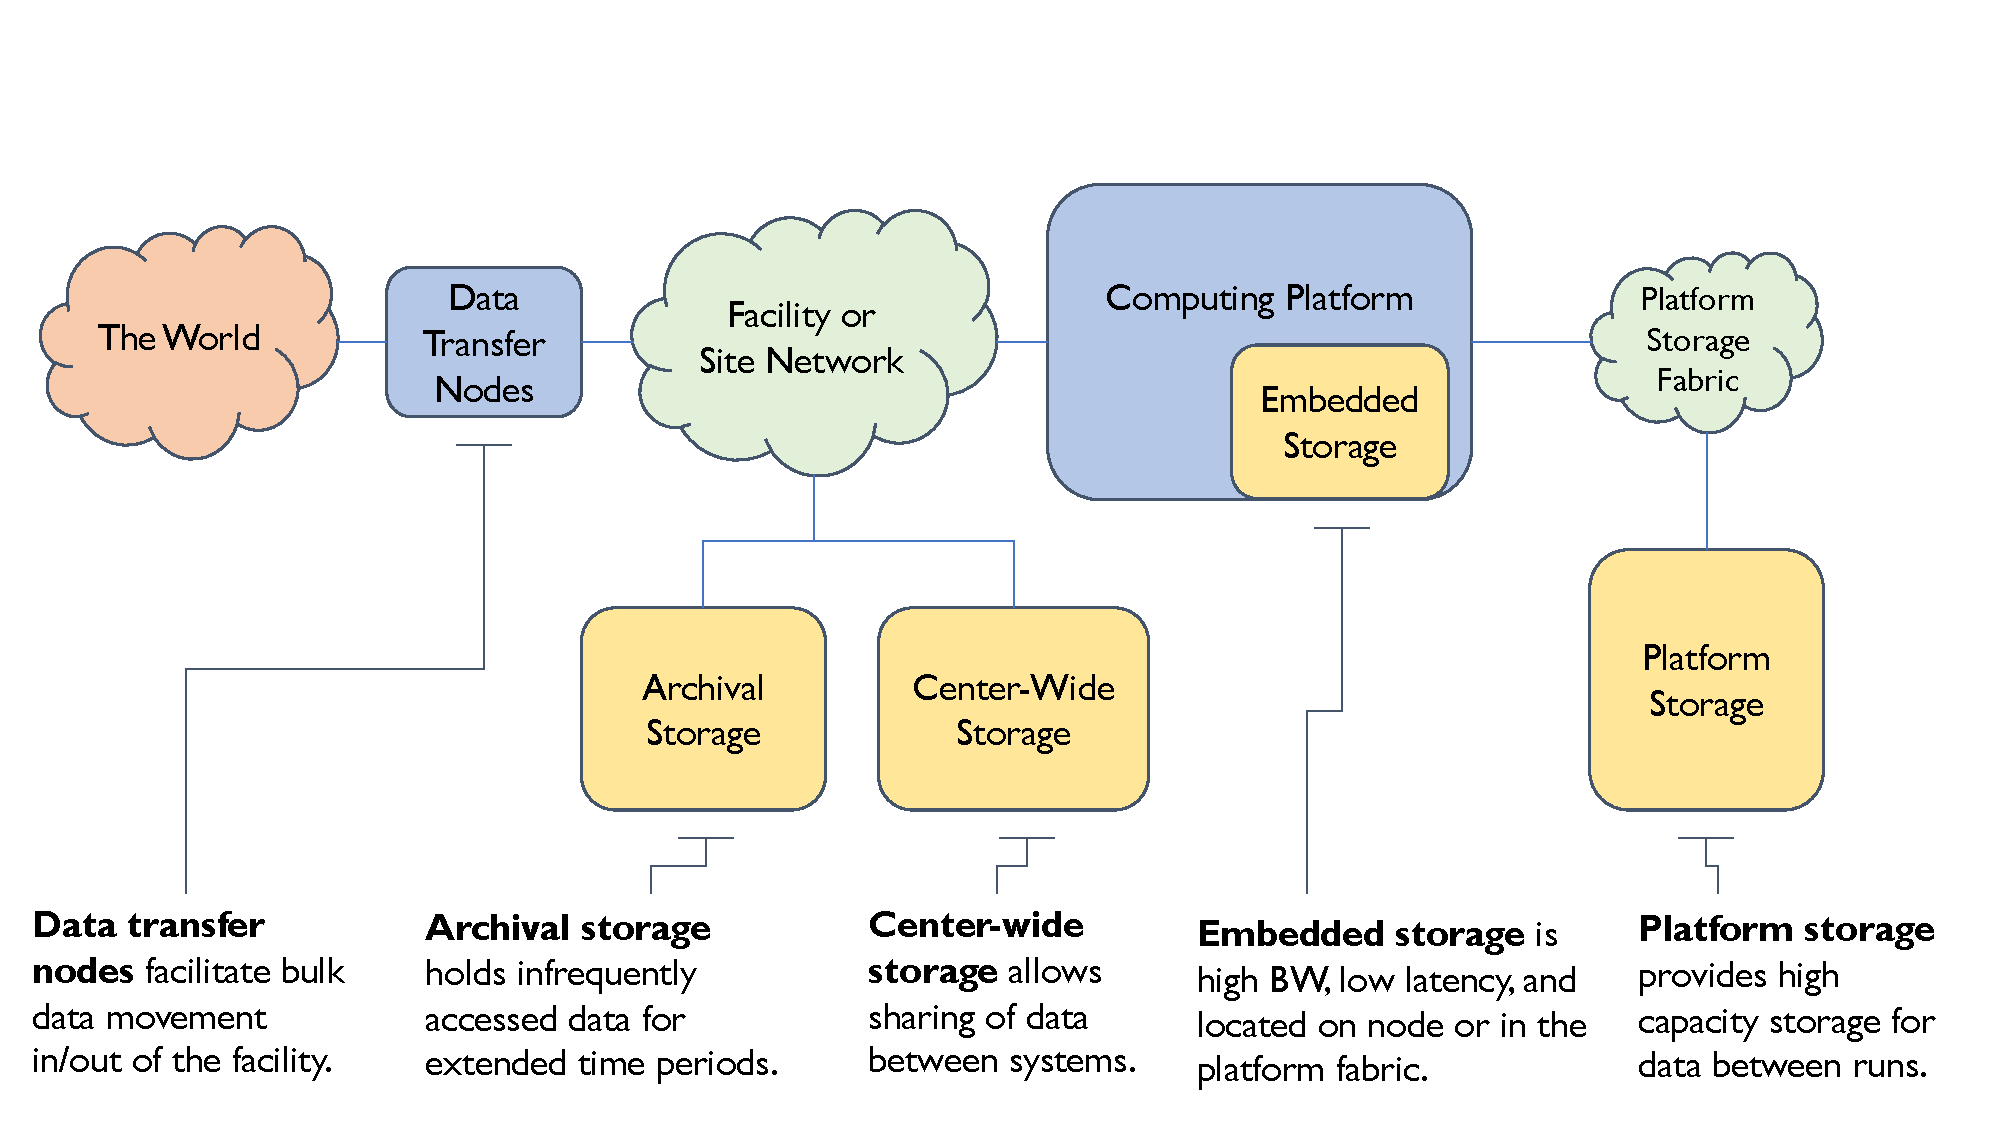
\includegraphics[width=0.70\textwidth]{projects/2.3.4-DataViz/DataViz-storage-notional-diagram.pdf}
	\caption{\label{fig:DataViz:StorageDiagram} A notional diagram of DOE
		facility storage resources. Not all systems have each role filled,
		and often additional network connections exist to accelerate specific
		data flows.}
\end{figure}


% FUTURE: STORAGE TECHNOLOGIES AND ARCHITECTURES
Figure~\ref{fig:DataViz:StorageDiagram} depicts a notional diagram of
the storage resources surrounding a leadership class platform at a DOE
facility. In this diagram, ``platform'' is the HPC system itself: Theta, Summit,
Cori, Frontier, Perlmutter, Aurora, etc. 

Note that this is a notional diagram. There are often additional
connections to speed specific transfers, and some sites augment one resource
while omitting another.
%
Data transfer nodes provide access to data stored on facility storage from the
outside world: Typically this is enabled using GridFTP, Globus Online, htar, or
similar.

There are lots of roles that storage might play:
\begin{itemize}
	\item \emph{Archival storage} holds ``cold'' data. Currently tape is
	still the dominant media for archival storage, but disk is also used,
	both as cache and as permanent storage (sometimes spun down).
	\item \emph{Center-wide storage} allows for easy data access between
	systems. This might include home directories and some other shared data
	volumes. Often performance is limited compared to platform storage.
	\item \emph{Platform storage} is storage that is connected to a limited
	number of platforms in the facility and is meant to be a high-performance,
	high-capacity store for data that will be used for multiple runs. While
	disk drives are still used in some platform storage deployments,
	increasingly solid-state storage (e.g., SSDs) is being employed in
	this role.
	\item \emph{Embedded storage} is located very close to the platform
	itself, either as node-local storage or tightly integrated into the
	fabric. Technologies used include NVMe and SSDs. Embedded storage that
	is available across the system is perhaps best thought of as a special 
	kind of platform storage.
\end{itemize}

%
% CURRENT STORAGE SPECS
%
\begin{table}[t]
	\vspace{-2mm}
	\centering
	\caption{\label{table:DataViz:StorageSpecsCurrent} Storage system specifications for current platforms.}
	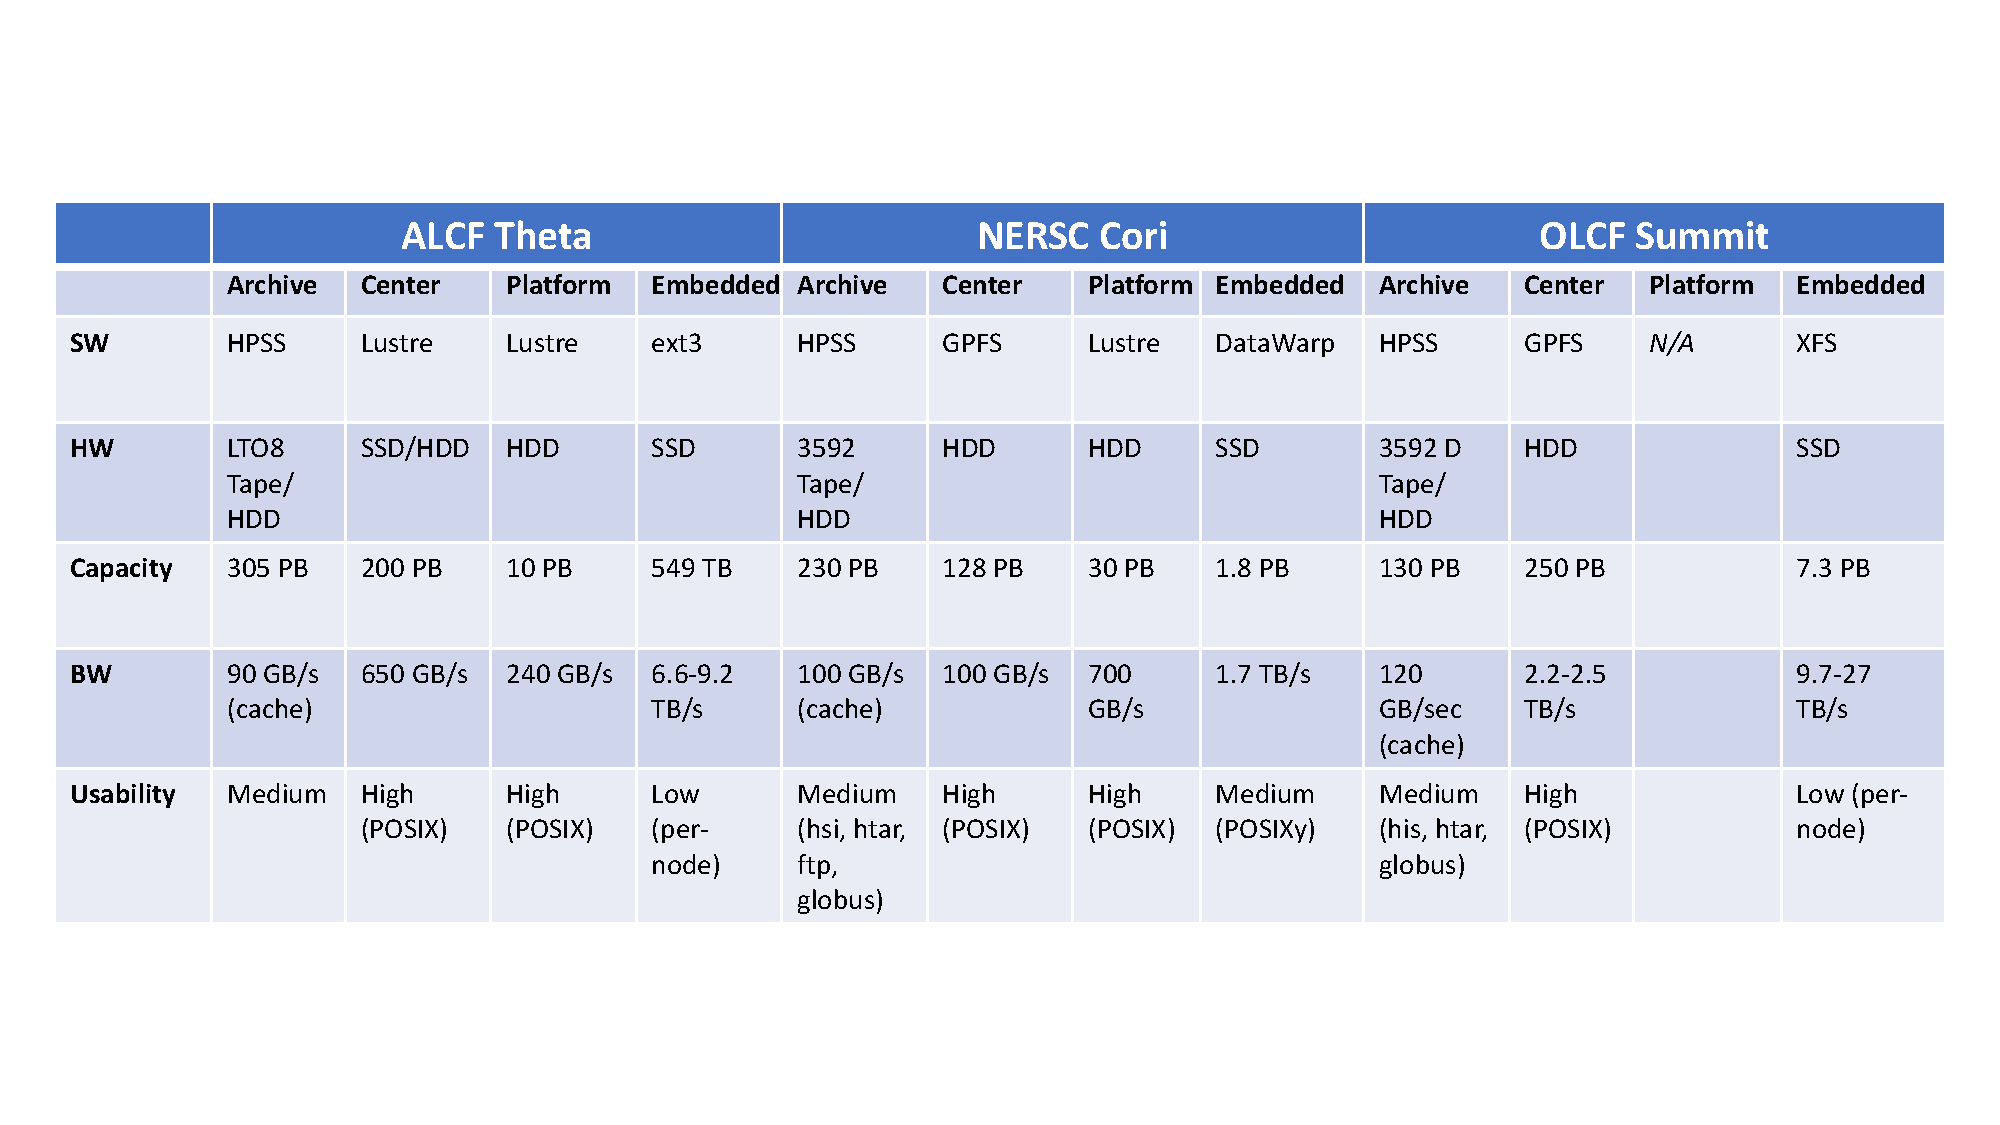
\includegraphics[width=0.75\textwidth]{projects/2.3.4-DataViz/DataViz-storage-specs-current.pdf}
\end{table}

Table~\ref{table:DataViz:StorageSpecsCurrent} captures the salient
characteristics of the storage deployments for the current generation of
systems: Theta, Cori, and Summit. These systems largely reflect trends in DOE
storage over the last decade: HPSS archival storage coupled with a POSIX
center-wide file system provided by GPFS or Lustre and backed by hard disk
drives (HDDs). In two cases a faster, platform-specific POSIX file system is 
deployed, while at OLCF the team chose to instead concentrate on a very high
performance center-wide file system that is available on other resources as well.

Of note in these systems are some embedded storage options that have
provided the community with some early experiences with SSD storage. On
Theta and Summit local SSDs are available that have seen limited use
by specific teams. On Cori, the DataWarp service allows for SSD-backed
storage pools to be allocated that are visible to an entire job or
workflow. This functionality is close to the model that users are
accustomed to, and the resource and has seen significant use.

%
% PROJECTED FUTURE SPECS
%
\begin{table}[t]
	\vspace{-2mm}
	\centering
	\caption{\label{table:DataViz:StorageSpecsNext} Projected storage specifications for upcoming platforms.}
	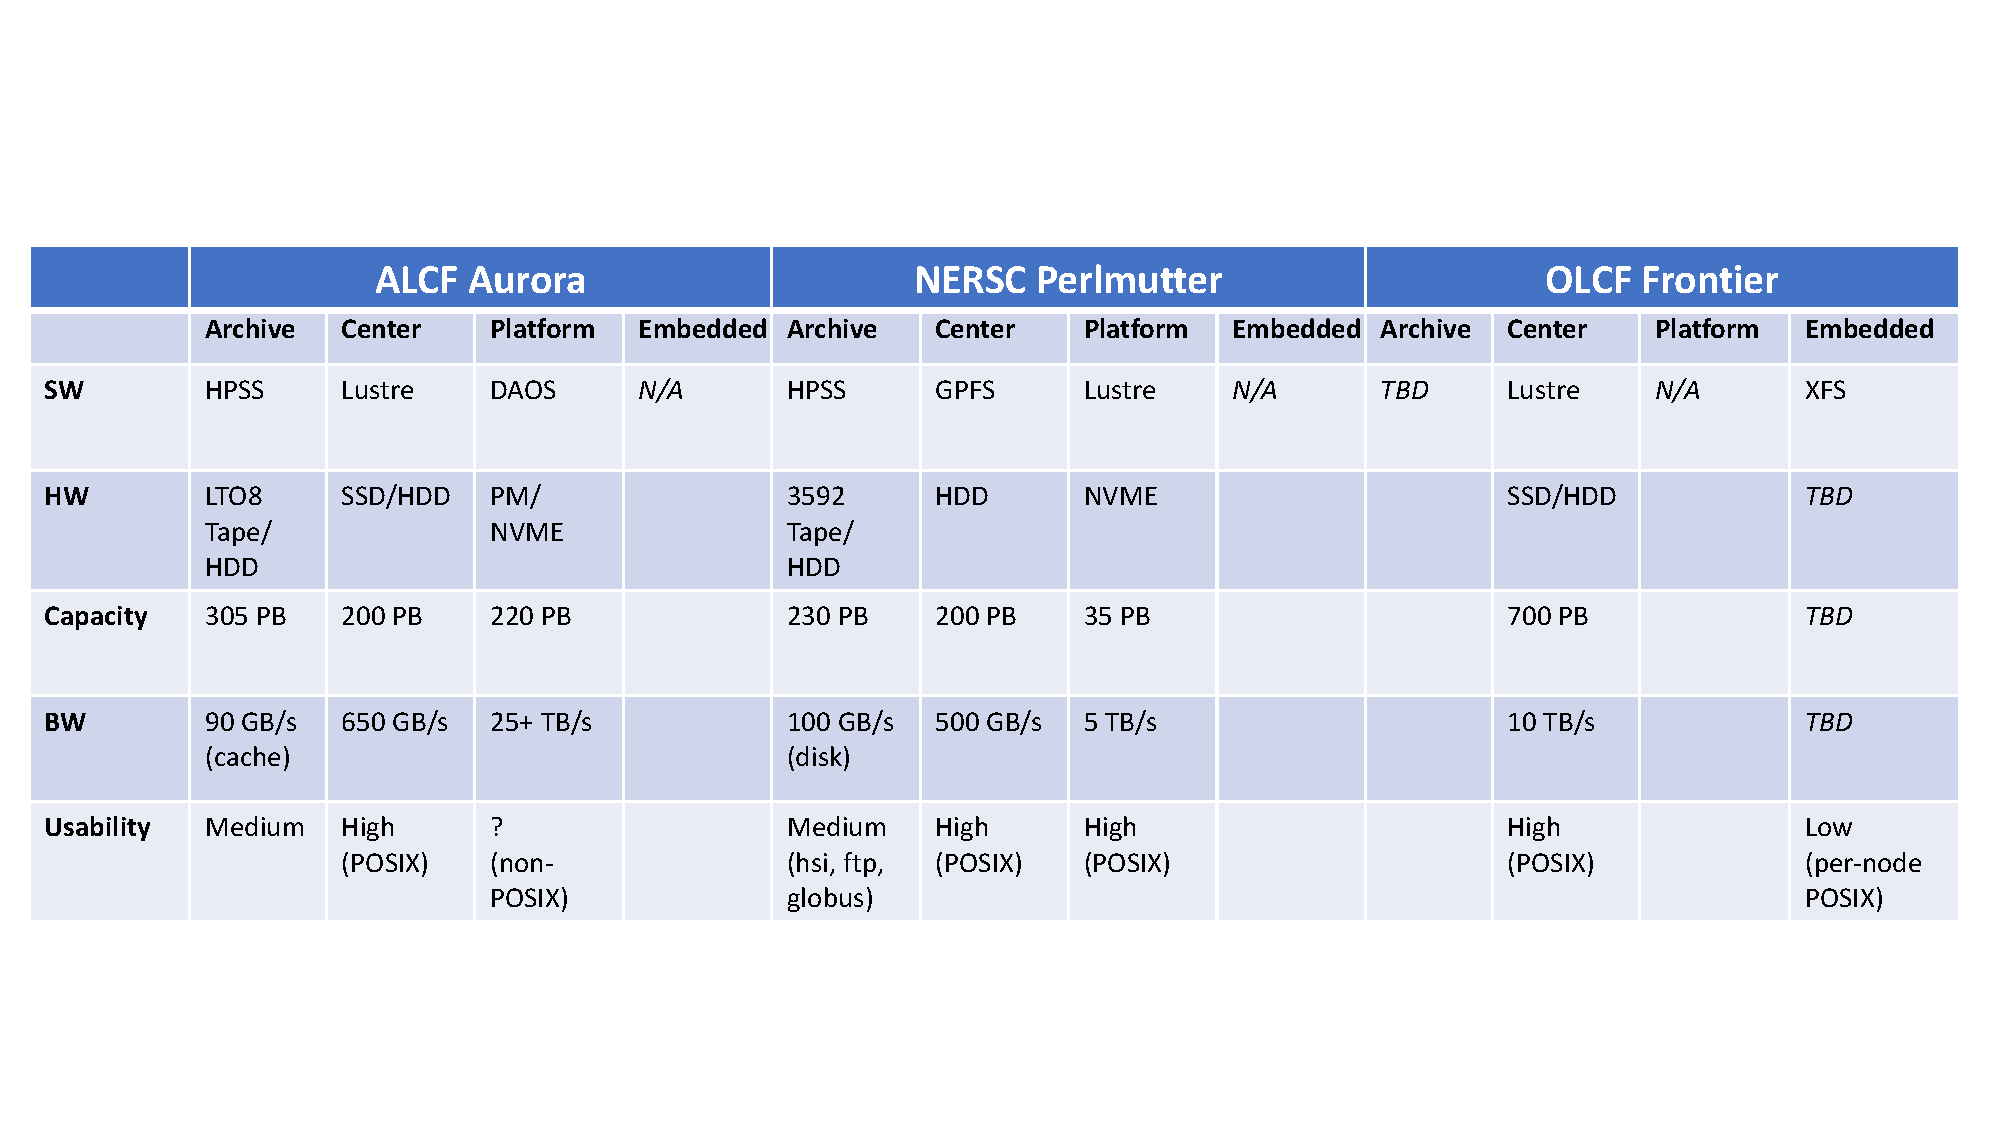
\includegraphics[width=0.75\textwidth]{projects/2.3.4-DataViz/DataViz-storage-specs-next.pdf}
\end{table}

Table~\ref{table:DataViz:StorageSpecsNext} captures the current, public
understanding of storage characteristics for the next generation of
systems: Aurora, Perlmutter, and Frontier.
%
Looking at this data, a number of observations can be made. First, POSIX will
remain the dominant (at least low-level) API for interacting with the primary
storage resources (embedded, platform, and center-wide). Obtaining peak
performance will likely remain a challenge for users, but with node counts
somewhat stalled, storage software scalability is not further pressured.
%
Second, a POSIX alternative, DAOS, will appear. DAOS is an Intel
product that will provide a form of globally accessible key-value
style of storage. However, a POSIX ``veneer'', or compatibility layer,
will be provided that will give users an easy way to make use of the
resource. With all the major ST I/O libraries already having the ability
to implement alternative back-ends, the challenge will be more about how
to persist things \emph{outside} DAOS efficiently (e.g., converting back
to POSIX files).
%
Finally, there will still be a non-global, embedded storage resource on
Frontier. The best ways to use this resource are unclear, but systems
like UnifyFS could play a role.


%\subsection{\stid{5} \ecosystem}\label{subsect:ecosystem}

\textbf{End State:} A production-ready software stack delivered to our facilities, vendor partners, and the open source HPC community.

\subsubsection{Scope and Requirements}
The focus of this effort is on the ``last mile'' delivery of software that is intended to be supported by DOE Facilities and/or vendor offerings. The scope of this effort breaks down into the following key areas:
\begin{itemize}
	\item Hardening and broad ST and facility adoption of Spack for easy build of software on all target platforms
        \item Delivery of formal software releases (E4S) in multiple packaging formats technologies -- from-source builds, modules, and containers
	\item Oversight of the ST SDKs developed in all five ST L3 areas, with a goal of ensuring the SDKs are deployed as production-quality products at the Facilities, and available to the broader open-source HPC community through coordinated releases
	\item Development of testing infrastructure (e.g., Continuous Integration) in collaboration with HI 2.4.4 (Software Deployment at the Facilities) for use by ECP teams at the Facilities
	\item Development and hardening of methods for software deployment through the use of container technology
	\item Development and hardening of a toolkit of reusable components for scientific workflow management systems
	\item Informal partnerships with the Linux Foundation's OpenHPC project for potential broader deployment of ST technologies in the OpenHPC ecosystem
\end{itemize}

A major goal of ST is to ensure that applications can trust that ST products will be available on DOE Exascale systems in a production-quality state, which implies robust testing, documentation, and a clear line of support for each product. This will largely be an integration effort building on both the SDKs project elements defined in each ST L3 area, and tight collaboration and coordination with the HI L3 area for Deployment of Software on Facilities (WBS 2.4.4). We will work to develop, prototype, and deliver foundational infrastructure for technologies such as continuous integration and containers in tight collaboration with our DOE facility partners. The ultimate goal is ensuring that the ECP software stack is robustly supported, as well as finding a reach into the broader HPC open-source community -- both of which provide the basis for long-term sustainability required by applications, software, Facilities, and vendors who rely upon these products.

Spack has broad adoption in the open-source community as an elegant solution toward solving many of the challenges presented by building software with many dependencies. Spack is one of the most visible outward-facing products in this L3 area, and is the basis for the SDK and E4S efforts.

\subsubsection{Assumptions and Feasibility}
Success in this effort will require a coordinated effort across the entire hardware and software stack –- in particular with HI 2.4.4 (Delivery of Software to Facilities) and in some cases, our vendor partners.  This cooperation is a critical first step in enabling our goals, and this area will drive toward ensuring those partnerships can flourish for mutual gain.

Given the project timelines and requirements of production systems at our Facilities, we do not envision a wholly new software stack as a feasible solution. We do however recognize that in many cases the software of today's HPC environments will very likely need to either be evolved or extended to meet the mission goals. This will require first, proof-of-concept on existing pre-Exascale hardware, and ultimately adoption of technologies by system vendors where required, and by other application and software teams.

\subsubsection{Objectives}
This area will focus on all aspects of integration of the ECP software stack embodied in E4S and the development of SDK Community Policies, and building the workflows community and deploying a toolkit of hardened, reusable components for workflow management systems, with a focus on putting the infrastructure in place (in partnership with HI and the SDKs) for production-quality software delivery through technologies such as Spack, continuous integration, and containers. 

\subsubsection{Plan}
Version 1.2 of the E4S was released in October, which includes 67 ST products that have Spack packages. This release is downloadable from DockerHub under the ecpe4s area.  The E4S Spack Build Cache now includes binaries for ppc64le as well as x86\_64 and includes over 22,000 total binaries.  The E4S containers now support custom images for ECP applications, such as WDMApp and Pantheon.  A regular cadence of E4S releases will continue, with updated ST products, broader facility adoption, and potentially inclusion in vendor offerings.

In close coordination with E4S, a number of SDKs are being developed across the other L3 ST areas, building on the years of experience the xSDK (Math Libraries).  These SDKs will become a prime vehicle for our delivery strategy, while also providing ST products with a standard set of community policies aimed at robust production-ready software delivery.  In October 2020, Version 1 of the E4S Community Policies was announced. The E4S Community Policies will serve as membership criteria for E4S member packages.  The E4S Community Policies will continue to evolve as we work toward release of Version 2 of them.

Spack continues to gain penetration across the ECP, and will be the de facto delivery method for ST products building from source. We provide Spack packaging assistance for ST users and DOE Facilities, and are developing new capabilities for Spack that enable automated deployments of software at Facilities, in containerized environments, and as part of continuous integration. A new effort to support running test suites within Spack environments via the {\tt spack test} functionality is underway and will be integrated with GitLab continuous integration to display dashboards for E4S tests.  Concurrently, we are developing technologies and best practices that enable containers to be used effectively at Facilities, and are pushing to accelerate container adoption within ECP.  

We filled a gap in the ST portfolio by instantiating a new project on scientific workflows, which is currently in an initial development phase.  Within this project, we are establishing the ExaWorks toolkit by assembling shared components from existing workflow projects. The ExaWorks toolkit will provide a robust, well-tested, documented, and scalable set of components that can be combined to enable diverse teams to produce scalable and portable workflows for a wide range of exascale applications. Importantly, the project will not create a new workflow system nor does it aim not to replace the many workflow solutions already deployed and used by scientists, but rather it will provide well engineered and scalable components which can be leveraged by new and existing workflows.

\subsubsection{Risks and Mitigation Strategies}
\begin{itemize}
	\item Deploying E4S on unknown architectures -- use Spack for deployment to decrease installation complexity
        \item Keeping updated versions of ST and dependent software in synch after initially achieving SDK interoperability
	\item Delays in deploying a common CI infrastructure lead to subsequent delays in an integrated software release
	\item Multiple container technologies in flight will make it hard to come to agreement on a ``common'' looking solution; may not be possible to generate containers that are both portable and performant
	\item ECP Application Reliance on workflow management systems that may not be scalable and performant at exascale -- mitigate by adopting robust, well-tested, and scalable components 
	\item OpenHPC partnership is ill-defined, and unfunded
	\item Sustainability of ECP ST capabilities after ECP has ended
\end{itemize}

\subsubsection{Future Trends}

SDKs will gain further traction in their communities as the benefits of 
interoperability and community policies are demonstrated.  We believe these processes will
become embedded into the communities and become one of the lasting legacies of ECP and
critical for sustainability beyond ECP.

Software deployments will continue to become more complex, especially when we require optimized 
builds for the unique and complicated exascale architectures.  Keeping dependencies updated and 
the software tested on these systems using continuous integration will tax the resources at 
the Facilities.  Software testing that includes interoperability and scalability tests will 
require further resources, both in terms of people to write the tests and the hours to
regularly run them.  These put greater emphasis on using and updating Spack as a
solution strategy for large collections of software and tight coordination with
HI and Facilities on CI infrastructure and resources.

Containers will become more popular and usable as a way to package the entire 
environment necessary to run an application on the exascale machines, thereby managing some of the 
complexity of an application deployment.  We expect that performance of an application within a 
container will be nearly as fast or faster than running the application on bare metal.  Application
build time will be reduced by using the associated build caches.

Workflows will continue to become more complex to complete their science missions, requiring
orchestration of many applications and scripts, executed at various scales across many 
different resource types, and often reliant on machine learning algorithms for guidance.
We expect that hardening workflow management systems and building a community centered
around robust and scalable components will be foundational for addressing these
complexities.  Moreover, we expect that container-based scientific workflows will 
begin to take off as we transition from demonstrations of applications at scale 
to performing science with them.


%\subsection{\stid{6} \nnsa}\label{subsect:nnsa}

\textbf{End State:} Software used by the NNSA/ATDM National Security
Applications and associated exascale facilities, hardened for
production use and made available to the larger ECP community.

\subsubsection{Scope and Requirements}
The NNSA ST L3 area was created in FY20, although the projects included
have all been part of the ECP before its creation. The capabilities of these
software products remains aligned with the other Software Technology
L3 areas from which they were derived, but are managed separately for
non-technical reasons out of scope of this document.

The resulting products in this L3 area 
are open source, important or critical to the success of the NNSA
National Security Applications, and are used (or potentially used) in
the broader ECP community. The products in this L3 span the scope of
the rest of ST (Programming Models and Runtimes, Development Tools,
Math Libraries, Data Analysis and Vis, and Software Ecosystem), and
will be coordinated with those other L3 technical 
areas through a combination of existing relationships and
cross-cutting efforts such as the ST SDKs and E4S.  

\subsubsection{Objectives}

The objective of these software products is to support the
development of new from-scratch applications within the NNSA that were
started just prior to the founding of the ECP under the ATDM (Advanced
Technology Development and Mitigation) program element within NNSA and
ASC. While earlier incarnations of these products may have been more
research-focused, by the time of the ECP ST restructuring in 2019 that
resulted in this L3 area, these products are in regular use by their
ATDM applications, and have matured to the point where they are ready
for use within the broader open source community.

\subsubsection{Plan}

NNSA ST products are developed with and alongside a broader
portfolio of ASC products in an integrated program, and are planned
out at high level in the annual ASC Implementation Plan, and in detail
using approved processes within the home institution/laboratory. They
are scoped to have 
resources sufficient for the success of the NNSA mission, as well as a
modicum of community support (e.g., maintaining on GitHub, or answering
occasional questions from the community).

For ECP products not part of the NNSA portfolio that have critical
dependencies on these products, there are often other projects within
ECP that provide additional funding and scope for those activities. In
those cases, there may be additional information within this document
on these products.


\subsubsection{Risks and Mitigation Strategies}

%A primary risk within this L3 area is that the 2020 ASC Level 1 milestone,
%designed as a capstone for the ATDM initiative and a decision point
%for the ultimate transition of those applications into the core ASC
%portfolio, will fail due to the inadequacy of these software
%products. While not all of them are on the critical path to
%application success (instead focusing on productivity enhancements for
%end users, or analysis functionality), it is expected that first and
%foremost they will contribute to the success of that milestone, as any
%subsequent ASC milestones and decision points about the ultimate fate
%of those applications. Mitigation is to use other ASC funding to bolster these
%efforts as needed.

One risk associated with the NNSA ST projects is the programming environment
of the El Capitan system. The programming environment on this system
will be a departure from what the NNSA software teams have used before,
so there is a risk that it will present challenges that cause delays
in porting the software to the system. That said, the probability of this risk is low because 
the programming environment of El Capitan will also be installed on DOE predecessor 
machines so it is likely that it challenges will be identified and addressed by
the time of El Capitan. NNSA ST projects can mitigate this risk by 
evaluating their software on the predecessor systems to identify challenges early.

Another risk associated with the NNSA ST L3 is that the projects rely
on multiple sources of funding outside of ECP. The budget priorities of 
those external sources may not always be aligned with those of ECP. In general,
this risk is low because the L4 leads strive to align their project goals across 
all funding sources. However, it is possible that funding expected to be leveraged
to develop a feature to later be used for ECP purposes may be dropped. If this 
occurs, the L4 leads will need to mitigate the situation according to their 
individual project needs, perhaps by renegotiating deliverable time lines.

Another risk is that others in the community will pick up these
products as open source, and expect additional support beyond the
scope of the primary NNSA mission. If those dependent products are within the
ECP, the main mitigation is to use ASCR contingency funding to provide
additional development and support - potentially through support of teams
outside of the home institution. If those dependent products are in
the broader community, mitigations are generally outside of the scope
of the ECP - although each NNSA lab typically has some sort of project
(or possibly even a policy) on how to deal with external demands on
open source products.





\newpage
\section{ECP ST Deliverables}\label{sect:deliverables}
\begin{wrapfigure}{r}{0.5\textwidth}
	\begin{mdframed}
		\large{ECP ST contributes to the HPC software ecosystem through direct product development, contributions to industry and de facto standards, and shaping the requirements, design, and prototyping of products delivery by vendors and other third parties.}
	\end{mdframed}
\end{wrapfigure}
ECP ST efforts contribute to the HPC software ecosystem in a variety of ways. The most tangible way was to include contributions to software products, many of which are already widely deployed and being transformed for use with exascale systems.  However, the ECP ST contributes to industry and de facto standards efforts.  Finally, some ECP ST efforts contribute to the upstream processes of requirements, analysis, design, and prototyping that inform the implementation of vendor and other third-party software products.  Although they do not receive the most attention, these upstream efforts are very impactful and low cost without a product to support.

%\begin{figure}[htb]
%	\begin{center}
%		\includegraphics[width=0.7\textwidth]{ProductsOverview}
%
%		\caption{\label{fig:productsoverview}{\small{The 33 ECP ST Projects contribute to 70 user-facing software product suites.   ECP ST products are delivered to users via many mechanisms. Provides experience we can leverage across projects.  Building via Spack is required for participating in ECP ST releases: 50 of the 70 ST product suites are available in the Extreme-scale Scientific Software Stack (E4S) V1.0, release in November 2019.}}}
%	\end{center}
%\end{figure}

\subsection{ECP ST Development Projects}\label{subsect:projects}
 ECP ST efforts support development in the following software projects spanning five technical areas: %(Table~\ref{table:wbs}).
 (1)~\pmr, see Table~\ref{table:pmr-products};
 (2)~\tools, see Table~\ref{table:tools-products};
 (3)~\mathlibs, see Table~\ref{table:math-products};
 (4)~\dataviz, see Table~\ref{table:vizdata-products}; and
 (5)~\ecosystem, see Table~\ref{table:eco-products}.
 Each table lists related projects, a URL (if available), and an estimate of deployment scope.

\begin{table}[H]
\centering
	\begin{tabular}{|l|l|l|}\hline
		\rowcolor{LightCyan}
		\textbf{Product} & \textbf{Website} & \textbf{Deployment scope}\\\hline
		GASNet-EX & \url{https://gasnet.lbl.gov} & Broad\\\hline
		Kokkos & \url{https://github.com/kokkos} & Broad\\\hline
		MPICH & \url{http://www.mpich.org} & Broad\\\hline
		OpenMPI & \url{https://www.open-mpi.org} & Broad\\\hline
		RAJA & \url{https://github.com/LLNL/RAJA} & Broad\\\hline

		CHAI & \url{https://github.com/LLNL/CHAI} & Moderate\\\hline
		Intel GEOPM & \url{https://geopm.github.io} & Moderate\\\hline
		Legion & \url{http://legion.stanford.edu} & Moderate\\\hline
		Qthreads & \url{https://github.com/Qthreads} & Moderate\\\hline
		Umpire & \url{https://github.com/LLNL/Umpire} & Moderate\\\hline
		UPC++ & \url{https://upcxx.lbl.gov} & Moderate\\\hline
		UMap & \url{https://github.com/LLNL/umap} & Moderate\\\hline
		Variorum & \url{https://github.com/LLNL/variorum} & Moderate\\\hline

		BOLT & \url{https://github.com/pmodels/bolt} & Experimental\\\hline
		Argobots & \url{https://github.com/pmodels/argobots} & Experimental\\\hline
		PaRSEC & \url{http://icl.utk.edu/parsec} & Experimental\\\hline
		AML & \url{https://xgitlab.cels.anl.gov/argo/aml} & Experimental\\\hline
		PowerSlurm & \url{https://github.com/tpatki/power-slurm} & Experimental\\\hline
	\end{tabular}
\caption{\label{table:pmr-products} \pmr~(18 total).}
\end{table}

\begin{table}[H]
	\begin{tabular}{|l|l|l|}\hline
		\rowcolor{LightCyan}
		\textbf{Product} & \textbf{Website} & \textbf{Deployment scope}\\\hline

		Caliper & \url{https://github.com/llnl/caliper} & Broad\\\hline
		Dyninst Binary Tools Suite & \url{http://www.paradyn.org} & Broad\\\hline
	 	Flang/LLVM Fortran compiler & \url{http://www.flang-compiler.org} & Broad\\\hline
		HPCToolkit & \url{http://hpctoolkit.org} & Broad\\\hline
		LLVM & \url{http://llvm.org/} & Broad\\\hline
		PAPI & \url{http://icl.utk.edu/exa-papi} & Broad\\\hline
		SCR & \url{https://github.com/llnl/scr} & Broad\\\hline
	    STAT & \url{https://github.com/LLNL/STAT} & Broad\\\hline
		TAU & \url{http://tau.uoregon.edu} & Broad\\\hline

		LLVM OpenMP compiler & \url{https://github.com/SOLLVE} & Moderate\\\hline
		OpenMP V \& V Suite & \url{https://bitbucket.org/crpl_cisc/sollve_vv/src} & Moderate \\\hline
		mpiFileUtils & \url{https://github.com/hpc/mpifileutils} & Moderate\\\hline
		openarc & \url{https://ft.ornl.gov/research/openarc} & Moderate\\\hline
		Papyrus & \url{https://csmd.ornl.gov/project/papyrus} & Moderate\\\hline
		Program DB Toolkit (PDT) & \url{https://www.cs.uoregon.edu/research/pdt} & Moderate\\\hline
	    PRUNERS Toolset & \url{https://github.com/PRUNERS/PRUNERS-Toolset} & Moderate\\\hline
		TriBITS & \url{https://tribits.org} & Moderate\\\hline

		Gotcha & \url{http://github.com/llnl/gotcha} & Experimental\\\hline
		Kitsune & \url{https://github.com/lanl/kitsune} & Experimental\\\hline
		Metall &  \url{https://github.com/LLNL/metall} & Experimental \\\hline
		QUO & \url{https://github.com/lanl/libquo} & Experimental\\\hline
		SICM & \url{https://github.com/lanl/sicm}  & Experimental \\\hline
		SuRF  & & Experimental\\\hline
\end{tabular}
\caption{\label{table:tools-products} \tools~(22 total).}
\todo[inline]{Please modify the preceding table to fit within the page margins.}
\end{table}


\begin{table}[H]
\begin{tabular}{|l|l|l|}\hline
		\rowcolor{LightCyan}
	\textbf{Product} & \textbf{Website} & \textbf{Deployment scope}\\\hline
	hypre & \url{http://www.llnl.gov/casc/hypre} & Broad\\\hline
	Kokkoskernels & \url{https://github.com/kokkos/kokkos-kernels} & Broad\\\hline
	MFEM & \url{http://mfem.org/} & Broad\\\hline
	PETSc/TAO & \url{http://www.mcs.anl.gov/petsc} & Broad\\\hline
	SLATE & \url{http://icl.utk.edu/slate} & Broad\\\hline
	SUNDIALS & \url{https://computing.llnl.gov/sundials} & Broad\\\hline
	SuperLU & \url{https://portal.nersc.gov/project/sparse/superlu} & Broad\\\hline
	Trilinos & \url{https://github.com/trilinos/Trilinos} & Broad\\\hline

	DTK & \url{https://github.com/ORNL-CEES/DataTransferKit} & Moderate\\\hline
	FleCSI & \url{http://www.flecsi.org} & Moderate\\\hline
	MAGMA-sparse & \url{https://bitbucket.org/icl/magma} & Moderate\\\hline
	STRUMPACK & \url{http://portal.nersc.gov/project/sparse/strumpack} & Moderate\\\hline
	xSDK & \url{https://xsdk.info} & Moderate\\\hline

	FFTX & \url{https://github.com/spiralgen/fftx} & Experimental\\\hline
	ForTrilinos & \url{https://trilinos.github.io/ForTrilinos} & Experimental\\\hline
	libEnsemble & \url{https://github.com/Libensemble/libensemble} & Experimental\\\hline
	Tasmanian & \url{http://tasmanian.ornl.gov} & Experimental\\\hline
	ArborX & \url{https://github.com/arborx/ArborX} & Experimental\\\hline
\end{tabular}
\caption{\label{table:math-products} \mathlibs~(18 total).}
\end{table}


\begin{table}[H]
\begin{tabular}{|l|l|l|}\hline
		\rowcolor{LightCyan}
	\textbf{Product} & \textbf{Website} & \textbf{Deployment scope}\\\hline
	Catalyst (ALPINE) & \url{https://www.paraview.org/in-situ} & Broad\\\hline
	Darshan & \url{http://www.mcs.anl.gov/research/projects/darshan} & Broad\\\hline
	HDF5 & \url{https://www.hdfgroup.org/downloads} & Broad\\\hline
	IOSS & \url{https://github.com/gsjaardema/seacas} & Broad\\\hline
	Parallel netCDF & \url{http://cucis.ece.northwestern.edu/projects/PnetCDF} & Broad\\\hline
	ParaView (ALPINE) & \url{https://www.paraview.org} & Broad\\\hline
	ROMIO & \url{http://www.mcs.anl.gov/projects/romio} & Broad\\\hline
	VeloC & \url{https://veloc.readthedocs.io} & Broad\\\hline
	VisIt (ALPINE) & \url{https://wci.llnl.gov/simulation/computer-codes/visit} & Broad\\\hline
	VTK-m & \url{http://m.vtk.org} & Broad\\\hline

	ADIOS & \url{https://github.com/ornladios/ADIOS2} & Moderate\\\hline
	ASCENT (ALPINE) & \url{https://github.com/Alpine-DAV/ascent} & Moderate\\\hline
	In Situ Algorithms (ALPINE) & \url{https://github.com/Alpine-DAV/algorithms} & Moderate\\\hline
	Cinema & \url{https://github.com/cinemascience} & Moderate\\\hline
	zfp & \url{https://github.com/LLNL/zfp} & Moderate\\\hline
	SZ & \url{https://github.com/szcompressor/SZ} & Moderate\\\hline

	C2C &  & Experimental\\\hline
	FAODEL & \url{https://github.com/faodel/faodel} & Experimental\\\hline
	GUFI & \url{https://github.com/mar-file-system/GUFI} & Experimental\\\hline
	HXHIM & \url{http://github.com/hpc/hxhim.git} & Experimental\\\hline
	MarFS & \url{https://github.com/mar-file-system/marfs} & Experimental\\\hline
	Mercury & \url{http://www.mcs.anl.gov/research/projects/mochi} & Experimental\\\hline
	ROVER & \url{https://github.com/LLNL/rover}   & Experimental\\\hline
	Siboka &  & Experimental\\\hline
	UnifyFS & \url{https://github.com/LLNL/UnifyFS} & Experimental\\\hline
\end{tabular}
\caption{\label{table:vizdata-products} \dataviz~(25 total).}
\todo[inline]{Please modify the preceding table to fit within the page margins.}
\end{table}



\begin{table}[H]
\centering
\begin{tabular}{|l|l|l|}\hline
		\rowcolor{LightCyan}
	\textbf{Product} & \textbf{Website} & \textbf{Deployment scope}\\\hline
	Spack & \url{https://github.com/spack/spack} & Broad\\\hline
	E4S & \url{https://e4s.io} & Broad\\\hline

\end{tabular}
\caption{\label{table:eco-products} \ecosystem~(two total).}
\end{table}

\newpage
\subsection{Standards Committees}
Participating in standards efforts is an important activity for ECP ST staff.  In many instances, the software will not be sustainable if it is not tightly connected to a standard. Additionally, any standard must account for the emerging requirements that exascale platforms need to meet to achieve performance and portability. Figure~\ref{fig:standards} summarizes ECP ST staff involvement in the major standards efforts that impact the ECP.

ECP ST staff are heavily involved in the MPI and OpenMP standards efforts and hold several key leadership positions within the standardizing bodies. ECP ST staff also play a critical role in C++ standards efforts. Although DOE staff have only recently engaged in C++ standards, ECP ST staff efforts are essential for ensuring that HPC requirements are considered, especially by contributing working code that demonstrates requirements and design. The ECP ST sponsors the newest open-source Fortran compiler, Flang~\ref{subsubsect:flang} as a front end for LLVM.  This compiler is rapidly emerging as an essential part of the HPC ecosystem.  In particular, although ARM processors are not explicitly part of the pre-exascale ecosystem, they are emerging as a strong contender in the future.  Flang is \textit{the} Fortran compiler for ARM-based systems.  ECP ST involvement in other committees provides valuable leverage and improved uniformity for HPC software.  Lastly, the Visualization Toolkit (VTK) Architecture Review Board (ARB) [...]\todo{Please complete this sentence.}.  Although this is only one instance, the team intends to explore the ARB model as part of its SDK efforts.
\begin{figure}[htb]
	\begin{center}
		\includegraphics[width=0.5\textwidth]{StandardsInvolvement}
		
		\caption{\label{fig:standards} ECP ST staff are involved in a variety of official and de facto standards committees.  Involvement in standards efforts is essential for ensuring the sustainability of ECT ST products and ensuring that emerging exascale requirements are addressed by these standards.}
	\end{center}
	\todo[inline]{Please convert this figure into a table.}
\end{figure}

\subsection{Contributions to External Software Products}\label{subsection:external-contributions}
Although many ECP ST efforts focus on the product that it will develop and support, some of the important work---and certainly some of the most sustainable and highly leveraged work---is done by providing requirements, analysis, design, and prototype capabilities to vendor and other third-party software.  Many software studies have shown that 70--80\% of the cost of a successful software product goes into post-delivery maintenance. The effort summarized in Table~\ref{table:externalproducts} expressly eliminates this large cost for DOE because the product is developed and supported outside DOE.


\begin{table}
	\begin{tabular}{|L{1.5in}|L{4in}|}\hline
			\rowcolor{LightCyan}
			Product & Contribution\\\hline
			Kokkos and RAJA & ECP efforts to provide portable on-node parallel programming and execution environments have led to new features in C++ standards. \\\hline
			MPI Forum & ECP ST staff maintain several chapters of the MPI Forum, an effort that requires constant involvement with the other authors, as well as participation in the online discussions related to the chapter and regular attendance of the MPI Forum's face-to-face activities.\\\hline
			Flang & ECP funds the development of the new open-source Fortran compiler front end called Flang. Flang provides Fortran language support for LLVM back ends in a way similar to how Clang provides support for C and C++.\\\hline 
			All \tools\ work & Starting in FY20, the \tools\ efforts are organized around delivering capabilities into the LLVM ecosystem.  \\\hline
			SWIG (www.swig.org) & The ECP ST ForTrilinos efforts contribute the capability to generate automatic Fortran bindings from C++ code.\\\hline
			TotalView debugger & ECP ST staff, along with RogueWave engineers, are engaged in the co-design of OMPD, the new debugging interface for OpenMP programs. This effort helps RogueWave improve its main debugging product, TotalView, by making it aware and compatible with recent advances in OpenMP debugging.\\\hline
			LLVM &  An ECP ST staff member is co-leading design discussions around the parallel intermediate representation (IR) and loop-optimization infrastructure.\\\hline
			SLATE & ECP ST Mathematical Library efforts inform the design, implementation, and optimization of dense numerical linear algebra routines on most vendor platforms.\\\hline
			Cray MPICH MPI-IO & As part of the ExaHDF5 ECP project, the ALCF worked with Cray MPI-IO developers to merge the upstream ROMIO code into the downstream proprietary Cray MPICH MPI-IO, leveraging Cray’s extensive suite of I/O performance tests and further tuning the algorithm.  Cray is currently targeting its deployment in an experimental release.\\\hline
			OpenHPC & An ECP ST staff member serves on the OpenHPC Technical Steering Committee as a component development representative.\\\hline
		\end{tabular}
		\centering
		\caption{\label{table:externalproducts} External products to which ECP ST activities contribute.  Participation in requirements, analysis, design, and prototyping activities for third-party products is some of the most effective software work that can be done.}
	\end{table}

%%ECP ST Product Dictionary
%Note: This page is still under construction.
%
%The ECP Software Technology (ST) Product Dictionary is the official list of publicly recognized 
%names to which ECP ST efforts contribute.  While ST teams use an expanded product 
%namespace, the list on this page indicates the eventual access point for ST product development 
%efforts.
%
%This table lists only those products that are typically recognizable to users. Examples:
%1.	MPI is commonly known by users. MPICH and OpenMPI both provide implementations 
%of that product.
%2.	Fortran is a product. Flang is a particular Fortran product. LLVM is a backend for some 
%Fortran compilers.
%3.	FFT is a product. FFTX, FFT-ECP provide FFT capabilities through interchangeable 
%interfaces. 
%4.	C++ is a product. Clacc provides capabilities for Clang, as does LLVM.
%
%Product 
%Dictionary 
%List
%ST products that deliver capabilities through public products 
%(comma separated list)
%
%ADIOS
%
%AML
%
%ALPINE: Ascent, ParaView, Catalyst, Visit, LibSim, In Situ Algorithms
%
%BLAS
%
%SLATE
%
%C
%
%LLVM
%
%C++
%
%LLVM
%
%Caliper
%
%Catalyst
%
%CHAI
%
%Cinema
%
%CUDA
%
%Darshan
%
%DTK
%
%Dyninst
%
%E4S
%
%FFT
%FFTX, FFT\_ECP
%FleCSI
%
%Flux
%
%Fortran
%LLVM/Flang
%GASNet
%
%Ginkgo
%
%HDF5
%
%HPCToolkit
%
%hypre
%
%Kokkos
%
%KokkosKernels
%
%LAPACK
%
%Legion
%
%libEnsemble
%
%MarFS
%
%MFEM
%
%MPI
%MPICH, Open MPI
%OpenACC
%Clacc/LLVM
%OpenCL
%-
%OpenMP
%SOLLVE/LLVM
%PAPI
%
%Papyrus
%
%Paraview
%
%PaRSEC
%
%PETSc/TAO
%
%PnetCDF
%
%PowerStack
%
%RAJA
%
%MPI-IO
%ROMIO
%ScaLAPACK
%SLATE
%SCR
%
%SICM
%
%Spack
%
%SPOT
%
%STRUMPACK
%
%SUNDIALS
%
%SuperLU
%
%SYCL
%
%SZ
%
%TASMANIAN
%
%TAU
%
%Trilinos
%
%UMap
%
%Umpire
%
%Unify
%
%UPC++
%
%VeloC
%
%VisIt
%
%VTK-m
%
%xSDK
%
%ZFP
%
%



%%---------------------------------------------------------------------------%%
%\vspace{3in}
\clearpage
%\newpage
\section{ECP ST Technical Areas}\label{sect:project-summaries}
%\section{ECP ST Project Summaries}\label{sect:project-summaries}

ECP ST is composed of six L3 technical areas (Figure~\ref{fig:l3-overview}).  This section of the report provides an overview of each L3 technical area and two-page summaries of each funded project within the technical area.  For each L3 area, the report discusses scope and requirements, assumptions and feasibility, objectives, plans, risks and mitigations, and future trends.  For each L4 subproject, a project overview is provided and the key challenges, solution strategy, recent progress, and next steps for the project are summarized.
\
\begin{figure}[H]
	\centering
	\fbox{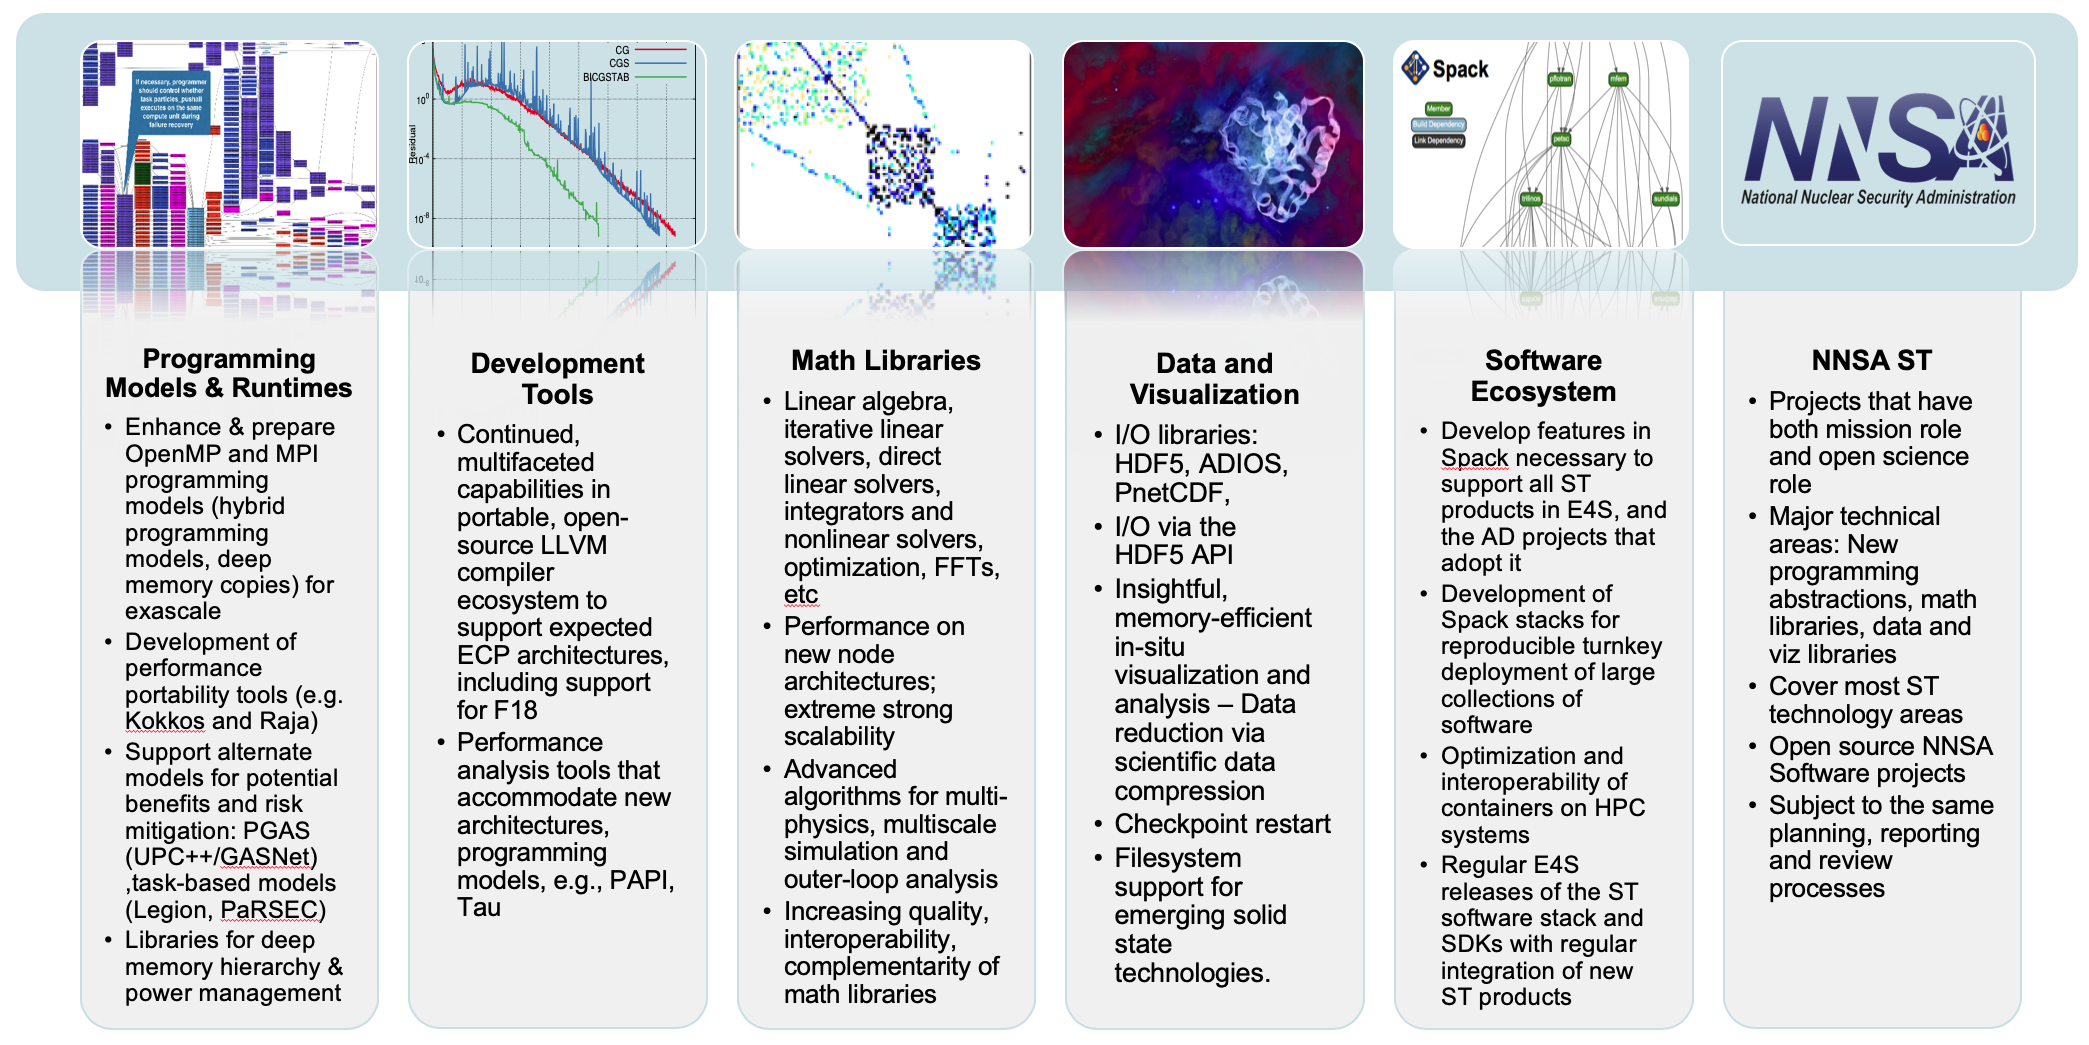
\includegraphics[width=0.9\linewidth]{L3-Overview}}
	\caption{ECP ST is composed of six L3 technical areas.  The first four areas are organized around functionality development themes.  The fifth is focused on technology for packaging and delivering capabilities.  The sixth is organized around per-lab open-source development at the three DOE NNSA laboratories: LANL, LLNL, and SNL.  }
	\label{fig:l3-overview}
	\todo[inline]{Please add a higher resolution version of this figure without the spell check underlines.}
\end{figure}

\newpage
%\subsection{\pmr}
%This section presents projects in \pmr.
\subsection{\stid{1}  \pmr}\label{subsect:pmr}

\textbf{End State:} A cross-platform, production-ready programming environment that enables and accelerates the development of mission-critical software at both the node and full-system levels.

\subsubsection{Scope and Requirements}
A programming model provides the abstract design upon which developers express and coordinate the efficient parallel execution of their program. A particular model is implemented as a developer-facing interface and a supporting set of runtime layers. To successfully address the challenges of exascale computing, these software capabilities must address the challenges of programming at both the node- and full-system levels. These two targets must be coupled to support multiple complexities expected with exascale systems (e.g., locality for deep memory hierarchies, affinity for threads of execution, load balancing) and also provide a set of mechanisms for performance portability across the range of potential and final system designs. Additionally, there must be mechanisms for the interoperability and composition of multiple implementations (e.g., one at the system level and one at the node level). This must include abilities such as resource sharing for workloads that include coupled applications, supporting libraries and frameworks, and capabilities such as in situ analysis and visualization. 

Given the ECP’s timeline, the development of new programming languages and their supporting infrastructure is infeasible. We do, however, recognize that the augmentation or extension of the features of existing and widely used languages (e.g., C/C++ and Fortran) could provide solutions for simplifying certain software development activities. 

\subsubsection{Assumptions and Feasibility}
The intent of the PMR L3 is to provide a set of programming abstractions and their supporting implementations that allow programmers to select from options that meet demands for expressiveness, performance, productivity, compatibility, and portability. It is important to note that, while these goals are obviously desirable, they must be balanced with an additional awareness that today’s methods and techniques may require changes in both the application and the overall programming environment and within the supporting software stack.

\subsubsection{Objectives}
PMR provides the software infrastructure necessary to enable and accelerate the development of HPC applications that perform well and are correct and robust, while reducing the cost both for initial development and ongoing porting and maintenance. PMR activities need to reflect the requirements of increasingly complex application scenarios, usage models, and workflows, while at the same time addressing the hardware challenges of increased levels of concurrency, data locality, power, and resilience. The software environment will support programming at multiple levels of abstraction that includes both mainstream as well as alternative approaches if feasible in ECP’s timeframe. 

Both of these approaches must provide a portability path such that a single application code can run well on multiple types of systems, or multiple generations of systems, with minimal changes. The layers of the system and programming environment implementation will therefore aim to hide the differences through compilers, runtime systems, messaging standards, shared-memory standards, and programming abstractions designed to help developers map algorithms onto the underlying hardware and schedule data motion and computation with increased automation.
\subsubsection{Plan}
PMR contains nine L4 projects. To ensure relevance to DOE missions, these efforts leverage and collaborate with existing activities within the broader HPC community. The PMR area supports the research and development needed to produce exascale-ready versions of the Message Passing Interface (MPI);  Partitioned Global-Address Space Libraries (UPC++, GASNet); task-based programming models (Legion, PaRSEC); software for node-level performance portability (Kokkos, RAJA); and libraries for memory, power, and resource management.
Initial efforts focused on identifying the core capabilities needed by the selected ECP applications and components of the software stack, identifying shortcomings of current approaches, establishing performance baselines of existing implementations on available petascale and prototype systems, and the re-implementation of the lower-level capabilities of relevant libraries and frameworks. These efforts provided demonstrations of parallel performance of algorithms on pre-exascale, leadership-class machines--at first on test problems, but eventually in actual applications (in close collaboration with the AD and HI teams). Initial efforts also informed research into exascale-specific algorithms and requirements that will be implemented across the software stack. The supported projects targeted and implemented early versions of their software on CORAL, NERSC and ACES pre-exascale systems--with an ultimate target of production-ready deployment on the exascale systems.
In FY20--23, the focus is on development and tuning for the specific architectures of the selected exascale platforms, in addition to tuning specific features that are critical to ECP applications.

Throughout the effort, the applications teams and other elements of the software stack evaluate and provide feedback on their functionality, performance, and robustness. Progress towards these goals is documented quarterly and evaluated annually (or more frequently if needed) based on PMR-centric milestones as well as joint milestone activities shared across associated software stack activities by Application Development and Hardware \& Integration focus areas.


\subsubsection{Risks and Mitigation Strategies}
The mainstream activities of ECP in the area of programming models focus on advancing the capabilities of MPI and OpenMP. Pushing them as far as possible into the exascale era is key to supporting an evolutionary path for applications. This is the primary risk mitigation approach for existing application codes. Extensions to MPI and OpenMP standards require research, and part of the efforts will focus on rolling these findings into existing standards, which takes time. To further address risks, PMR is exploring alternative approaches to mitigate the impact of potential limitations of the MPI and OpenMP programming models. 

Another risk is the failure of adoption of the software stack by the vendors, which is mitigated by the specific delivery focus in sub-element SW Ecosystem and Delivery. Past experience has shown that a combination of laboratory-supported open-source software and vendor-optimized solutions built around standard APIs that encourage innovation across multiple platforms is a viable approach and is what we are doing in PMR. We are using close interaction with the vendors early on to encourage adoption of the software stack, including well-tested practices of including support for key software products or APIs into large procurements through NRE or other contractual obligations. A mitigation strategy for this approach involves building a long-lasting open-source community around projects that are supported via laboratory and university funding. 

Creating a coordinated set of software requires strong management to ensure that duplication of effort is minimized. This is recognized by ECP management, and processes are in place to ensure collaboration is effective, shortcuts are avoided unless necessary, and an agile approach to development is instituted to prevent prototypes moving directly to product. 

\subsubsection{Future Trends}
Recently announced exascale system procurements have shown that the
trend in exascale compute-node hardware is toward heterogeneity:
Compute nodes of future systems will have a combination of regular
CPUs and accelerators (typically GPUs). Furthermore, the GPUs will not
be just from NVIDIA as on existing systems: One system will have Intel
GPUs and another will have AMD GPUs. In other words, there will be a
diversity of GPU architectures, each with their own vendor-preferred
way of programming the GPUs. An additional complication
is that although the HPC community has some experience in using NVIDIA
GPUs and the associated CUDA programming model, the community has relatively
little experience in programming Intel or AMD GPUs.  These
issues lead to challenges for application and software teams in
developing exascale software that is both portable and high performance. Below
we outline trends in programming these complex systems that will help
alleviate some of these challenges.

\paragraph{Trends in Internode Programming}
The presence of accelerator hardware on compute nodes has resulted in individual
compute nodes becoming very powerful. As a result, millions of compute
nodes are no longer needed to build an exascale system. This trend
results in a lower burden on the programming system used for internode
communication. It is widely expected that MPI will continue to serve
the purpose of internode communication on exascale systems and is the
least disruptive path for applications, most of which already use
MPI. Nonetheless, improvements are needed in the MPI Standard as well
as in MPI implementations in areas such as hybrid programming
(integration with GPUs and GPU memory, integration with the intranode
programming model), overall resilience and robustness, scalability,
low-latency communication, optimized collective algorithms, optimized support
for exascale interconnects and lower-level communication paradigms
such as OFI and UCX, and scalable process startup and management. PGAS
models, such as UPC++ and OpenSHMEM, are also available to be used by
applications that rely on them and face similar
challenges as MPI on exascale systems. These challenges are being tackled by the MPI and
UPC++/GASNet projects in the PMR area.

\paragraph{Trends in Intranode Programming}
The main challenge for exascale is in achieving performance and portability for
intranode programming, for which a variety of options
exist. Vendor-supported options include CUDA and OpenACC for NVIDIA
GPUs, SYCL/DPC++ for Intel GPUs, and HIP for AMD GPUs. OpenACC
supports accelerator programming via compiler directives. SYCL
provides a C++ abstraction on top of OpenCL, which itself is a
portable, lower-level API for programming heterogeneous
devices. Intel's DPC++ is similar to SYCL with some extensions. HIP
from AMD is similar to CUDA; in fact, AMD provides translation tools
to convert CUDA programs to HIP.

Among portable, standard programming models, OpenMP has supported
accelerators via the \texttt{target} directive starting with OpenMP version
4.0 released in July 2013. Subsequent releases of OpenMP (version 4.5
and 5.0) have further improved support for accelerators. OpenMP is
supported by vendors on all platforms and, in theory, could serve as a
portable intranode programming model for systems with
accelerators. However, in practice, a lot depends on the quality of
the implementation.

Kokkos and RAJA provide another alternative for portable,
heterogenous-node programming via C++ abstractions. They
are designed to work on complex node architectures
with multiple types of execution resources and multilevel memory
hierarchies. Many ECP applications are successfully using Kokkos and
RAJA to write portable parallel code that runs efficiently on GPUs.

We believe these options (and high-quality implementations of them) will
meet the needs of applications in the exascale timeframe. 

\newpage

\subsubsection{\stid{1.01} \pmr\ Software Development Kits} 

\paragraph{Overview} 
The \pmr\ SDK effort is focused on identifying meaningful aggregations of products in this technical area.  SDK efforts are in the early stages of planning and execution.  Most of the work on SDKs has been driven from the \ecosystem\ technical area.  A description of the SDK effort can be found in Section~\ref{subsubsect:ecosystem-sdk}.

\newpage
\subsubsection{\stid{1.07} Exascale MPI} \label{subsubsect:mpich}
\paragraph{Overview}

MPI has been the de facto standard programming model for HPC from the
mid 90's till today, a period where supercomputing performance
increased by six orders of magnitude.  The vast majority of DOE's
parallel scientific applications running on the largest HPC systems
use MPI. These application codes represent billions of dollars of
investment. Therefore, MPI must evolve to run as efficiently as
possible on Exascale systems. Our group at Argonne developed a
high-performance, production-quality MPI implementation, called MPICH.
The focus areas of the Exascale MPI / MPICH project are: (1)
continuous improvement of the performance and capabilities of the
MPICH software to meet the demands of ECP and other broader DOE
applications, (2) coordinate vendor and supercomputing center
interactions to ensure efficient solutions to applications, and (3) be
involved in the MPI Forum and standardization efforts to ensure
continuity of the work beyond this project.

The MPICH group was involved in the formation of the MPI Forum and has been
deeply involved in defining the MPI standard since 1992. MPICH has
helped prototype and define the majority of the features in the MPI
standard. As such, MPICH has been one of the most influential pieces of
software in accelerating the adoption of the MPI standard by the HPC
community. MPICH has been adopted by leading vendors into their own
derivative implementations. Examples include Intel (for Intel MPI), Cray
(for Cray MPI), IBM (for IBM PE MPI), Mellanox (for MLNX-MPI), Microsoft
(for MS-MPI), and Ohio State University (for MVAPICH). MPICH and its
derivatives are routinely used in the majority of the top 10 supercomputers in
the world. MPICH is the recipient of a number of awards including
an R\&D 100 award.

\paragraph{Key Challenges}

While we believe MPI is a viable programming model at Exascale, both
the MPI standard and MPI implementations have to address the
challenges posed by the increased scale, performance characteristics
and evolving architectural features expected in Exascale systems, as
well as the capabilities and requirements of applications targeted at
these systems. The key challenges are:

\begin{enumerate}

\item Interoperability with intranode programming models having a high
  thread count~\cite{Hybrid1, Hybrid2, FT2} (such as OpenMP,
  OpenACC and emerging asynchronous task models);

\item Scalability and performance over complex
  architectures~\cite{FT2, Perf1, Perf2, Perf4} (including high core
  counts, processor heterogeneity and heterogeneous memory);

\item Software overheads that are exacerbated by lightweight cores and
  low-latency networks;

\item Enhanced functionality (extensions to the MPI standard) based on
  experience with applications and high-level libraries/frameworks
  targeted at Exascale; and

\item Topics that become more significant as we move to the next
  generation of HPC architectures: memory usage, power, and
  resilience.

\end{enumerate}

\paragraph{Solution Strategy}

The Exascale MPI project has the following primary technical thrusts:
(1) \textbf{Performance and Scalability} (2) \textbf{Heterogeneity}
(3) \textbf{Topology Awareness} (4) \textbf{Fault Tolerance} and (5)
\textbf{MPI+X Hybrid Programming}.

Our solution strategy started by addressing performance and
scalability aspects in MPICH related to network address
management~\cite{memscal}.  Apart from this, we also looked at
communication strategies which allow the MPI library to be as
lightweight as possible~\cite{ch41, ch42}. Other solutions include
investigation and evaluation of communication relaxation hints,
investigation of optimizations to memory scalability in MPICH and
improvements to MPI RMA operations.

Exascale MPI heterogeneity efforts~\cite{Hetero1, Hetero2, Hetero3}
started with the survey on heterogeneous memory architectures on
upcoming DOE machines and how MPICH can take advantage of
them~\cite{hexe}. The efforts also included the investigation of
utilizing heterogeneous memory inside the MPI implementation and
evaluation of applications~\cite{hetero4}. The heterogeneity efforts
further extended to investigating and developing technologies for GPU
integration for the better support of the coming Exascale
supercomputers.

Exascale MPI topology awareness efforts~\cite{Topo1,Topo2} originated
with the investigation and evaluation of hints based on topology
awareness and optimizations to virtual topology functionality in
MPICH~\cite{topo-io,topo-io2}. The other efforts include investigation
of topology-aware collectives and neighborhood collectives in
MPICH~\cite{coll} and evaluation of the selected ECP applications.

Exascale MPI fault tolerance efforts~\cite{FT1, FT2} started with
support for handling noncatastrophic errors in MPI. The second effort
included defining the scope of errors in MPI, a prerequisite for
user-level failure mitigation. Other efforts in this direction
include standardizing these efforts in MPI and evaluating application
suitability for fault tolerance.

Exascale MPI+X hybrid programming efforts involved
improving interoperation of MPICH with threads~\cite{interthread}.
Secondly, we developed the work-queue data transfer model for
multithreaded MPI communication~\cite{workq}. We have included support
for interaction of MPICH with user-level thread (ULT)
libraries~\cite{ULT}, primarily targeting Argobots and the BOLT
runtime~\cite{BOLT}.  Other issues being investigated include the
design and evaluation of multiple virtual communication
interfaces (VCIs) for multithreaded MPI communication~\cite{VCI}.

\paragraph{Recent Progress}

One major achievement of MPICH recently is the support for the newly
released MPI-4 standard. The MPI-4 standard introduced new ways for
communication including persistent collective that aims to reduce the
overhead of repetitively setting up collective, and partitioned
communication which aims to improve the performance for multi-threaded
MPI communication. The MPICH 4.0 release has include all the new MPI-4 
features.

We focus on better GPU support in MPICH. MPICH now supports
GPUs from all three vendors (NVIDIA, AMD and Intel). The support for
GPU communication includes a fast path that utilizes the hardware RDMA
support for GPU memory, and a fallback path for cases like complex
datatypes which cannot be directly handed by hardware RDMA. We have
also developed prototypes for GPU-stream-triggered operations, which allow
an MPI application to enqueue MPI point-to-point communication to a GPU
stream or command queue. This allows the GPU stream to be used to manage
the synchronization between GPU kernels and the MPI communication that
depends on the result of those kernels. The benefit includes better
overlapping between computation and communication, and higher GPU
utilization.

\paragraph{Testing, Continuous Integration, and Experience on Early
Access Systems}

Validation and verification has been an integral part of the MPICH
project. We have made several improvements to the automated testing
infrastructure for more effective testing. Specifically, we added the
support for testing with GPU buffers for all three GPU vendors. It
enables us to test MPI communications with different combinations of CPU
and GPU buffer including inter-process communication between multiple
GPUs on the same node. We regularly test MPICH using both Spock and
Arcticus to evaluation and verify the new features and optimizations
that targets the upcoming exascale systems. We have also setup a
Continuous Integration (CI) configuration to automate part of the test.
These testing and verification helped us identify problems early and
provides the necessary environment for experiments. It also simplifies
our collaborations with vendor partners that we have similar hardware
setup for testing on issues of common interests.

%\begin{figure}[htb]
%  \centering
%  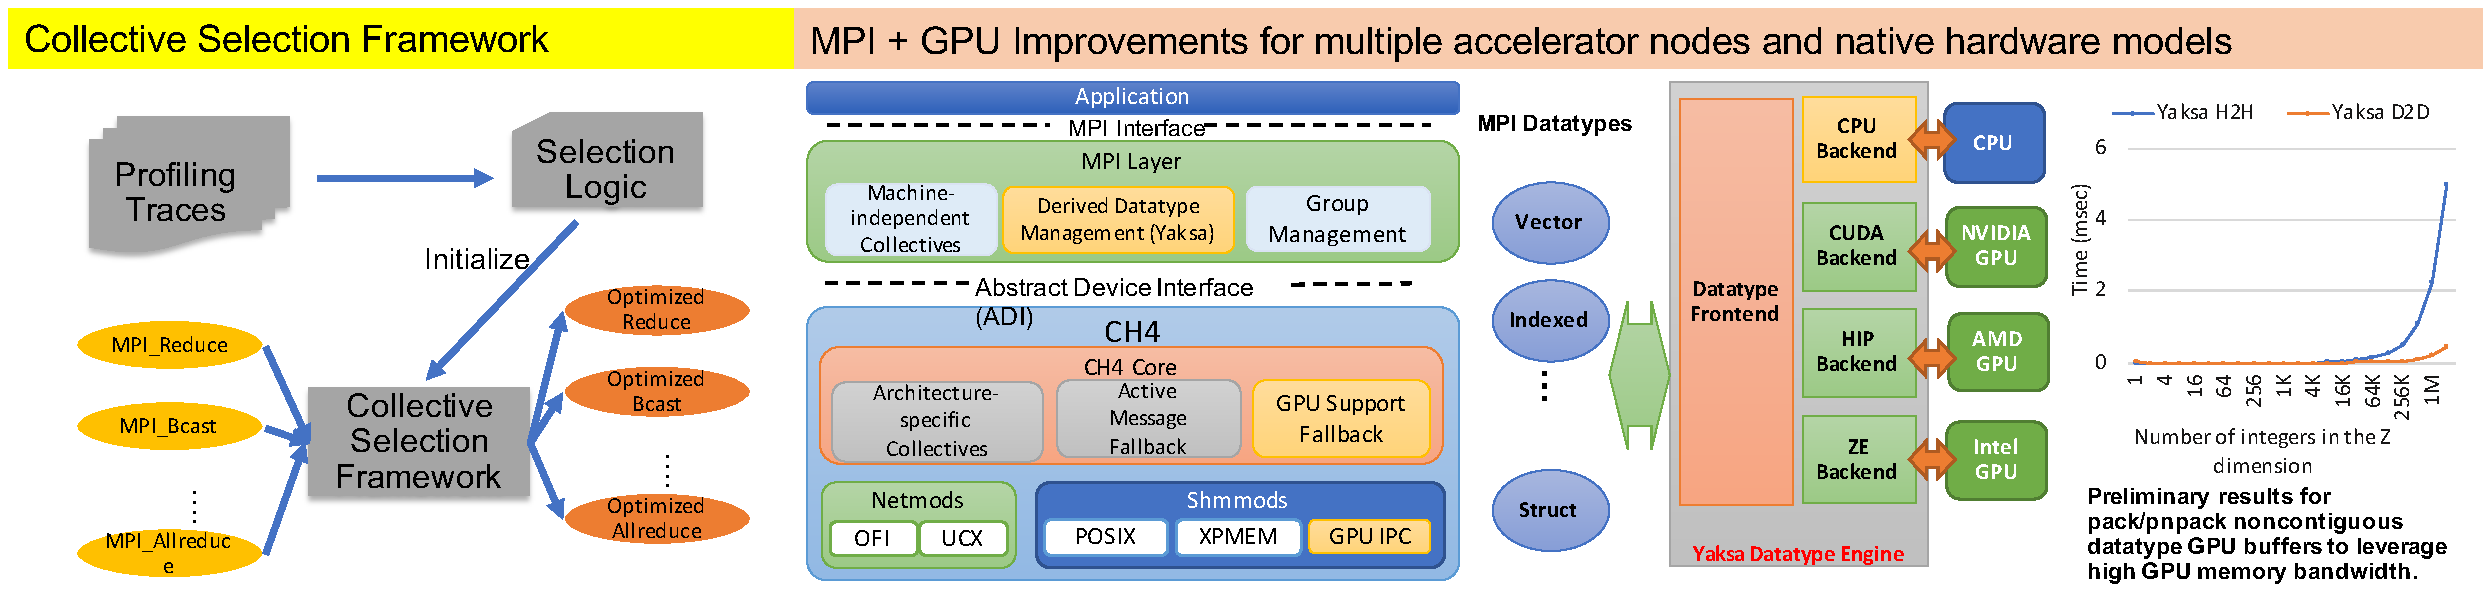
\includegraphics[width=6in]{projects/2.3.1-PMR/2.3.1.07-Exascale-MPI/MPICH-recent-milestones.pdf}
%  \caption{\label{fig:fy20}Major MPICH milestones completed in fiscal year 2020}
%\end{figure}

\paragraph{Next Steps}
In the next year, we plan to continue optimizing the GPU support in
MPICH. Planned work includes performance evaluation and improvement of GPU
communication, support for GPU collectives, and  extending
GPU-stream-triggered operations to more MPI communication functions.
We will also expand the software validation and verification work on
pre-exascale and exascale systems to make MPICH perform well on the target
machines. We will also continue our close collaboration with the
vendors, Intel and Cray, to ensure that high-quality MPICH-based MPI implementations
(Intel MPI and Cray MPI) are available on the exascale platforms.

\newpage
\subsubsection{\stid{1.08} Legion}

\paragraph{Overview}
This project focuses on the development, hardening and support of the
Legion Programming System (\url{https://legion.stanford.edu}) with a
focus on Exascale platforms and workloads that can benefit from
Legion's features and capabilities.  At a fundamental level, the
project focuses s on the key capabilities (e.g. correctness,
performance, scalability) of an alternative programming model for ECP
that seeks to expose additional levels of parallelism and provide more
flexible data-centric abstractions.  In addition, Legion also enables
a separation of concerns of the implementation of an application from
how it is mapped onto a given system architecture.

Our efforts have been focused on addressing bugs, refactoring the
implementation for improved stability, performance and scaling,
extending support for the selected exascale platforms, and also
expanding the feature set as needed for both application and
platform requirements.

\paragraph{Key Challenges}
As with all new approaches to programming high-performance systems,
there is a distinct challenge and a significant level-of-effort required to
reach a level of stability, capabilities, and performance to establish
stability, acceptance, and an established user base.  In this
regard, Legion is becoming more widely used outside of ECP for both
machine-learning and data-centric workloads within industry (e.g.,
NVIDIA and Facebook).  This growing base is providing both additional
developers and use cases that are helping to stabilize the code as
well as broaden the overall scope of testing.  Much like these efforts
benefit from ECP Legion-centric efforts, ECP is benefiting from this
growth and additional external investments.

We have focused much of our efforts on emerging use cases within ECP
that are a mix of traditional workloads, and those related to machine
learning (ML) and data-centric computation.  The data-centric and ML
domains have provided a path for more substantial impact given reliance
on external tools (e.g. TensorFlow, Python, etc.) vs. years of established code
written in MPI.  We continue to see clear benefits from focusing our efforts in
these areas. This has helped us to increase our overall impact as well focus on
areas of adoption across more specialized application needs that seeks to leverage
machine learning and related workloads.

The ML component is support primarily via the FlexFlow framework that
is discussed in more detail below. FlexFlow represents an additional
level of scope that require its own set of efforts for hardening,
expanding the feature set, tuning performance, and porting to the ECP
target platforms.  None of the FlexFlow scope was originally planned at the
outset of ECP. 

\paragraph{Solution Strategy}
As part of a larger collaboration between LANL, Stanford University,
NVIDIA, SLAC, Facebook, MIT, and others this project provides the
overarching implementation of Legion that captures the most stable
(correct, feature complete, and performant) versions of the programming
system for ECP's use.  In addition, we are actively looking for
opportunities to further educate the broader community about Legion 
and general advantages of using data-centric and task-based approaches
to programming.

We have continued working with Ristra (AD 2.2.5.01), ExaFEL (AD
2.2.4.05) and the CANDLE project (AD 2.2.4.03) to provide support for
Legion.  For all these efforts we provide support, software releases,
and bug fixes related to both correctness and performance. Our project
includes management of the current repository and quarterly, or more
frequent, releases of Legion to the broader community (e.g. NVIDIA,
Facebook, FlexFlow, etc.).  In addition, we have provided initial
support for AMD and Intel GPUs, and features that support
inter-operation with other languages and programming systems --
e.g. MPI, OpenMP, Kokkos, Fortran, and Python. Finally, we have collaborated
at the lower levels of the software stack with the GASNet-EX effort (part
of the Pagoda project in ST).

As part of the focused work with CANDLE, we are providing additional
support with the implementation of the FlexFlow deep-learning
framework that is built on top of Legion.  This framework has proven to
be significantly faster than industry-provided solutions such as TensorFlow
and PyTorch -- providing over a 15x reduction in training time on some of
CANDLE's networks. 

\paragraph{Recent Progress}

We continue to discover and address both performance and scalability
issues in the runtime.  In addition, for use cases within ECP, and
also a growing set of users outside of ECP, we have continued to
identify and address bugs and other issues (e.g. missing features).
The vast majority of these fixes have been released and are part of
the Legion releases in use within ECP.

Additional work, some done in collaboration with the GASNet-EX team, has provided a Legion implementation that
supports AMD's GPU architectures as well as GPU-to-GPU network-based
communications.  In addition, the Kokkos interoperability support in
Legion now also supports AMD's GPU software stack and testing is
underway with the Ristra team for full support on early access
test-beds for AMD-based exascale platforms.  Performance debugging will
be an upcoming activity once appropriate resources are available.

Additional work has been done to support Intel's GPUs and all of
Legion's internal CI tests and small test applications are
successfully and correctly running on early access systems.
Performance debugging will be an upcoming activity once appropriate
resources are available.

We have continued to develop high-level entry points for FlexFlow that
allow it to seamlessly use code from existing learning frameworks (e.g.,
Keras, PyTorch, and ONNX).  We currently have versions of Keras/TensorFlow
networks running correctly and are continuing to make progress on support
for PyTorch and ONNX.   Additional work has been done to improve performance
via exposing new levels of parallelism in training networks as well as
graph-centric optimizations.  Our latest results suggest a 2-3x performance
boost over previous results for one of CANDLE's example learning networks.
Like Legion, we currently use a quarterly set of releases for FlexFlow that
are aligned to leverage features and new capabilities of Legion and the
underlying software components on the target platforms. 

Both FlexFlow and Legion are open source projects and distributed via GitHub:

\begin{itemize}
  \item Legion: \url{https://github.com/StanfordLegion/legion/}
  \item FlexFlow: \url{https://github.com/flexflow/FlexFlow} 
\end{itemize}

\paragraph{Next Steps}

Our plans for the next year are to continue focusing on the challenges
presented by obtaining reliable, high performance versions of Legion and
FlexFlow on the upcoming exascale system architectures.  

We will continue to work on the Python interfaces for Legion (an aspect
of growing interest from the ExaFEL project for improved productivity)
and the feature set of FlexFlow requested by CANDLE.  This will include
seeking out and improving our outreach and leveraging new features of
Legion exposed by other non-ECP efforts.  Regular open-source releases of
Legion and FlexFlow will continue, and as we test on the early access
systems we will continue to focus on bug fixes, improving capabilities and 
developer productivity, and addressing performance issues. 





\newpage
\subsubsection{\stid{1.09} Distributed Tasking at Exascale: PaRSEC}


\paragraph{Overview}

The PaRSEC Environment provides a software ecosystem composed of a runtime
component to dynamically execute task-based applications on heterogeneous
distributed systems, and a productivity toolbox that comprises a development
framework for the support of multiple Domain Specific Languages (DSLs) and
extensions, with debugging, trace collection, and analysis tools.
%
\begin{wrapfigure}[17]{l}{.45\linewidth}
\includegraphics[scale=0.3]{projects/2.3.1-PMR/2.3.1.09-ParSEC/PaRSEC-diagram.png}
\caption{PaRSEC\label{fig:parsec} modular framework allows each
component to be dynamically activated.}
\end{wrapfigure}
%
The PaRSEC project team is dedicated to solving two challenging and
interdependent problems facing the ECP developer community: First, how to create
an execution model that enables developers to express as much parallelism as
possible in their applications, so that applications effectively utilize the
massive collection of heterogeneous devices ECP machines will deploy. Second,
how to ensure the execution model is flexible and portable enough to actually
provide and sustain a performance benefit by increasing the scientific
productivity of the application developers, not only for the ECP target
environments but for the foreseeable future.

PaRSEC is an open source, community-based implementation of a generic task-based
runtime that is freely available, and used by an increasing number of software
libraries.
%  The PARSEC development team is mainly comprised of research staff at % UTK,
%  but regular contributions from the community are provided via our presence %
%  on GitHub and Bitbucket.
The project focuses on providing a stable and efficient infrastructure for quick
prototyping of different approaches to define task-based languages able to
exploit the full range of capabilities of Exascale platforms. Without such a
project, and based on the current state of task-based runtime, potential users
will be stuck either in fixed programming paradigms, or with a particular,
potentially less efficient, mix of programming languages. The DTE project
provides means to maintain a high competitiveness in the field leading to more
innovation on addressing the challenges we are facing toward scalable,
efficient and Exascale-ready programming paradigms.

\paragraph{Key Challenges}
%\textit{Describe what is hard to do, why it is challenging.}

As we get closer to the delivery of Exascale platforms, an increasing number of
aspects of the hardware and software environment still pose challenges. First
and foremost, keeping pace with the architectural changes on current and future
platforms requires changes not only on how we take advantage of the hardware
capabilities, but how we reshape our algorithms and applications to expose
enough parallelism to maximize the use of the underlying hardware. The number of
nodes, threads per node, memory hierarchies and support for increased
computational capabilities (accelerators) will continue to increase, while the
currently available programming paradigms are still struggling with parallelism
at the node level.

\begin{wrapfigure}{l}{.45\linewidth}
\centering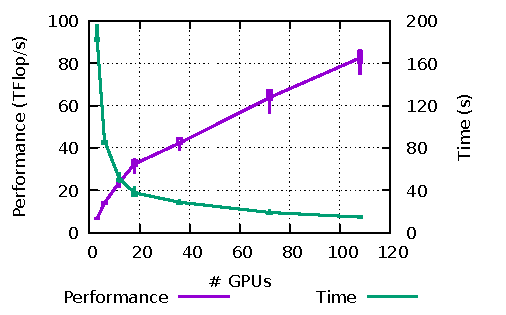
\includegraphics[width=.9\linewidth]{projects/2.3.1-PMR/2.3.1.09-ParSEC/irr-bs-gemm-combined.pdf}
\caption{Time to solution and Performance as a function of the number
  of V100 GPUs on Summit, for the molecule
  $C_{65}H_{132}$\label{fig:irrbsgemm}}
\end{wrapfigure}\paragraph{Solution Strategy}
%\textit{Describe your basic strategy for addressing the challenges.}
The approach followed in PaRSEC is to provide a low-level, flexible and dynamic
runtime able not only to schedule tasks at the node level, but to handle data
transfers between different memory (both inter- and intra-nodes), memory
hierarchies, heterogeneous architectures with support for accelerators with a
simple programming scheme. The proposed approach envisions a middle-ground
solution, addressing both hardware and software challenges. At the hardware
level a team of dedicated developers extends PaRSEC to map its capabilities to
the hardware and to improve its scalability and performance. At the upper
software level the runtime interactions are through Domain Specific Languages
with the target domain scientists in mind, that will facilitate the expression
of algorithmic parallelism with familiar constructs mapped on the exposed
low-level capabilities. To facilitate the integration of PaRSEC-driven libraries
into larger and complex applications, PaRSEC natively interoperate with other
programming paradigms, including some target of the ECP PMR support, such as
PGAS, MPI, OpenMP and Kokkos. This integration provides a smooth transition for
library developers that embrace the PaRSEC runtime, providing a platform where a
shift to a new programming paradigms can be done in stages of increased
complexity~\cite{lorapo-protools,BLR_LU,parsec_pdgemm}.
% In this model, PaRSEC remains in full control of data tracking and
% allocation on the managed accelerator.


%
% Recent work: irregular block-sparse GEMM on Summit
%


The PaRSEC team, in collaboration with NWChemEx project researchers,
developed an efficient and portable tensor product algorithm
specifically designed for the computational chemistry domain needs on
top of the PaRSEC runtime. This includes an efficient matrix product
operation for hybrid architectures (such as Summit) with an irregularly
blocked, block-sparse representation of matrices. Moreover, the
requirements on this implementation were extremely strict, the
matrices are rectangular and extremely large in at least one of their
dimensions, such that none of the input matrices could fit in the
aggregated memory of all GPUs. The algorithm and a deeper analysis of
the results are described in~\cite{parsec::rr::irrbs}.

\begin{wrapfigure}[16]{l}{.45\linewidth}
\vspace*{-1.5em}\centering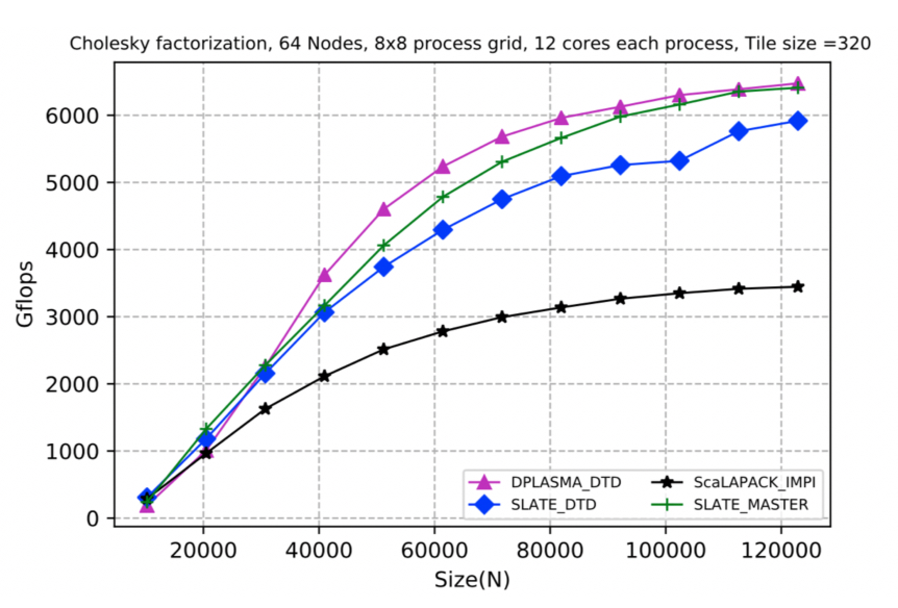
\includegraphics[scale=0.50]{projects/2.3.1-PMR/2.3.1.09-ParSEC/slate_updated_nacl.pdf}
  \caption{Comparison of DPLASMA and SLATE Cholesky factorization over PaRSEC with
           SLATE and ScaLAPACK on 64 nodes 12 cores each\label{fig:slate-parsec}}
\end{wrapfigure}

Figure~\ref{fig:irrbsgemm} shows a strong scaling performance
evaluation of this algorithm, when applied to the main tensor product
required by the CCSD method to simulate the electronic structure from
first principles. The simulated molecule was $C_{65}H_{132}$, which is
a quasi-1-dimensional system and small atomic orbital basis, where the
sparsity of tensors is maximized while the optimal (from the data
compression perspective) tile size is small. That molecule is
representative of applications to 1-d polymers and quasi-linear
molecules (such as some proteins), while the choice of the atomic
orbital basis is representative of medium-precision simulations in
chemistry and condensed phase. Such use case stresses the system and
algorithm as it implies a significant sparsity: the largest matrix,
while being of square of rank $2,464,900$, has only a density of
3.1\%.

The strong scaling evaluation shows a parallel efficiency of 35\%,
with a time to solution at 180s on 3 GPUs, going down to 13s at 118
GPUs.
% The performance per GPU decreases with the number of nodes,
% between 36\% at 3 GPUs and 12\% at 118 GPUs.
Compared to the state of the art, DBCSR~\cite{parsec::dbcsr} can only
run problems that fit in the GPU memory, preventing us to run the same
experiment, but experiments on synthetic problems that fit in memory
show an improvement by a factor two, while
TiledArray~\cite{parsec::tiledarray} cannot leverage the GPUs of
Summit without using PaRSEC and would run, on the CPUs of Summit ten
times slower.
%
% End
%


An important aspect of the DTE project is to define and prototype scalable
domain specific languages that enable a productive expression of parallelism for
end-user communities. PaRSEC presents multiple programming interfaces
(Parameterized Task Graphs for maximum parallelism, the popular serial task
insertion dataflow model to provide direct access to the runtime). In addition,
the DTE team is in close contact with application teams to define parallel
abstractions that are suitable for their domain usage. Notably, the PaRSEC team
has ongoing collaboration with the SLATE linear algebra package and NWChemEx and
GAMESS chemistry package teams.

In this context it is interesting to highlight the first step toward
the integration of the PaRSEC framework into the SLATE (2.3.3.09) in
the context of the shared milestone (STPM11-23). The first prototype
of the application ran in a distributed environment and showed the
capability of the SLATE library using a modern fully capable runtime
system. This work involved enhancing the insert task interface
available in the PaRSEC runtime to map onto the logic of a SLATE
algorithm.

Figure~\ref{fig:slate-parsec} compares different implementation of the
Cholesky factorization. On one side we have two reference
implementations for distributed linear algebra, ScaLAPACK and the
current version of the SLATE library (using OpenMP for intra-node
parallelism and MPI for communications). On the other side we have two
DSL expressing the same algorithm but using PaRSEC as the underlying
runtime, the Dynamic Task Discovery (DTD) an approach similar to
OpenMP but working on a distributed setting, and a version of the
SLATE library where instead of relying on explicit parallelism
(OpenMP) and communications (MPI) it rely on implicit dependencies
management via PaRSEC.


% side including the integration of SLATE and PaRSEC. Two domain
% specific languages that have the capability to do linear algebra; then
% against the regular SLATE using OpenMP for intra-node parallelism, and
% MPI for communication; and finally against ScaLAPACK, which is the
% reference for distributed linear algebra.

%
% Recent work: ScaLAPACK - DPLASMA - PaRSEC
%


%\begin{wrapfigure}{l}{.42\linewidth}
%\centering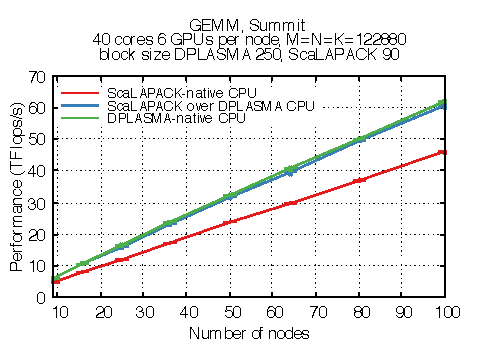
\includegraphics[width=.9\linewidth]{projects/2.3.1-PMR/2.3.1.09-ParSEC/scalapack_cpu_GEMM.pdf}
%\centering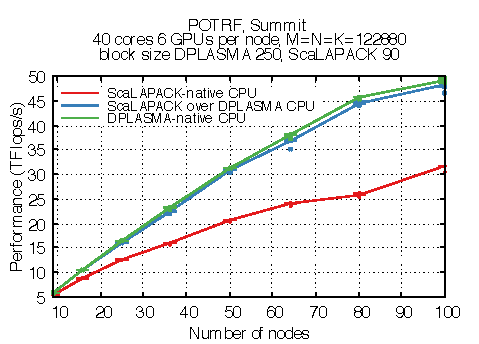
\includegraphics[width=.9\linewidth]{projects/2.3.1-PMR/2.3.1.09-ParSEC/scalapack_cpu_POTRF.pdf}
%\caption{Performance using only CPUs of native ScaLAPACK, ScaLAPACK
%  over DPLASMA and native DPLASMA for GEMM and
%  POTRF.\label{fig:scalapack_cpu}}
%\end{wrapfigure}
%\begin{wrapfigure}{l}{.42\linewidth}
%\centering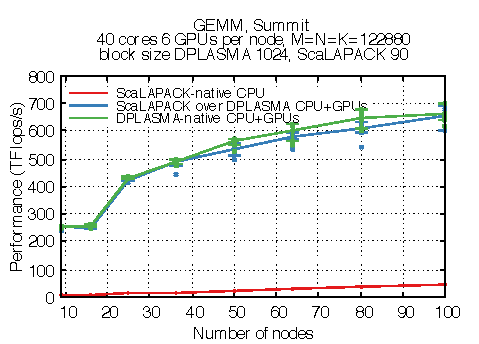
\includegraphics[width=.9\linewidth]{projects/2.3.1-PMR/2.3.1.09-ParSEC/scalapack_gpu_GEMM.pdf}
%\centering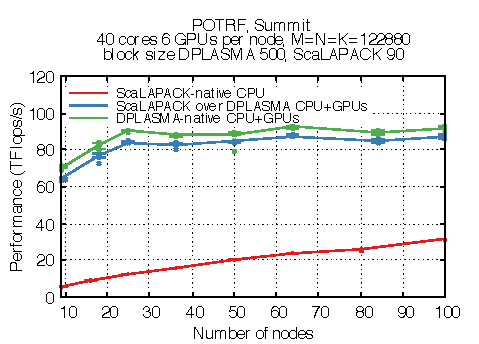
\includegraphics[width=.9\linewidth]{projects/2.3.1-PMR/2.3.1.09-ParSEC/scalapack_gpu_POTRF.pdf}
%\caption{Performance using GPUs of native ScaLAPACK, ScaLAPACK over
%  DPLASMA and native DPLASMA for GEMM and
%  POTRF.\label{fig:scalapack_gpu}}
%\end{wrapfigure}
\begin{wrapfigure}{l}{.45\linewidth}
\centering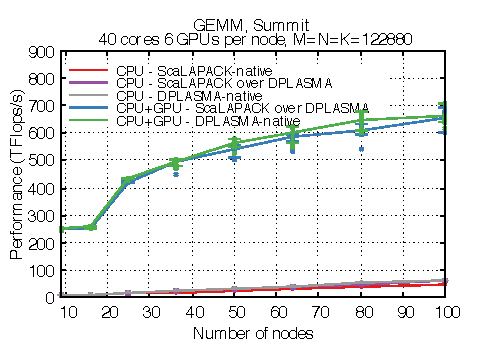
\includegraphics[width=.9\linewidth]{projects/2.3.1-PMR/2.3.1.09-ParSEC/scalapack_GEMM.pdf}
\centering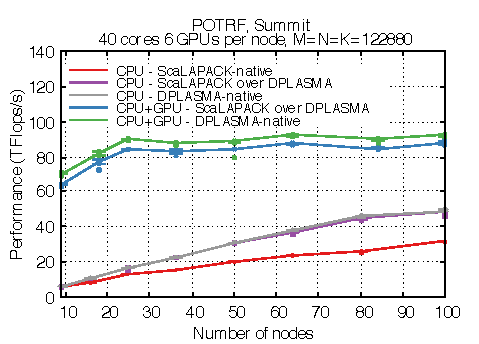
\includegraphics[width=.9\linewidth]{projects/2.3.1-PMR/2.3.1.09-ParSEC/scalapack_POTRF.pdf}
\caption{Performance using GPUs of native ScaLAPACK, ScaLAPACK over
  DPLASMA and native DPLASMA for GEMM and
  POTRF.\label{fig:scalapack_gpu}}
\end{wrapfigure}
In the context of milestone STPM11-81, the PaRSEC team worked to
enable the usage DPLASMA as a replacement for ScaLAPACK.  This
functionality is provided as an independent library which contains a
wrapped version of the ScaLAPACK API and hides the PaRSEC API from the
application while it constructs the structures necessary for the
operation with matrices represented on ScaLAPACK memory layout.  Users
of applications exploiting ScaLAPACK can link against this independent
library to run the wrapped routines over DPLASMA-PaRSEC, while any
other ScaLAPACK function, i.e. that does not have an equivalent
provided by DPLASMA, will use the original ScaLAPACK implementation.
This approach reduces to a minimum the changes that need to be
performed on the ScaLAPACK application, while enabling the
exploitation of the algorithms implemented on DPLASMA and the
operation over PaRSEC for a better exploitation of the available
hardware resources.


Figure~\ref{fig:scalapack_gpu} compare the
performance of the ScaLAPACK wrapper extensions against the native
DPLASMA and native ScaLAPACK in their typical usage scenarios (one
process per core for ScaLAPACK),
% Experiments were run using a dense matrix with dimensions 122~880 in
% double precision. The internal block size and the process grid have
% been tuned for the best performance on each library. In all cases,
% the native ScaLAPACK tests were ran spawning one process per core
while DPLASMA tests (native DPLASMA and ScaLAPACK over DPLASMA) use
one thread per core and one process per node on the experiments using
only the CPU and two processes per node, each exploiting 3 GPUs, are
used on the GPU tests.
%
In all cases, the performance achieved by running ScaLAPACK over
DPLASMA is more than 90\% the performance of native DPLASMA.  For the
CPU-only experiments, the usage of the DPLASMA wrapper introduces a
speedup of 1.73x for GEMM (minimum 1.64x, maximum 1.88x) and 1.49x for
POTRF (minimum 1.27x, maximum 1.71x) .  When exploiting also the GPUs
of the computation nodes, the performance is increased by 16.75x for
GEMM (minimum 10.79x, maximum 25.68x) and by 4.27x for POTRF (minimum
2.77x, maximum 6.70x).  The lower performance of the DPLASMA's POTRF
over GPUs is explained because in the current implementation of this
algorithm not all the tasks are run on GPUs. However, further
improvements of DPLASMA algorithms that will be integrated in the next
release of DPLASMA will likely achieved similar performance when used
for wrapping the ScaLAPACK routines. Therefore, enabling applications
already using the ScaLAPACK API to improve their usage of the
available hardware resource with very little effort that is translated
in important performance benefits.

%
% End
%


\paragraph{Recent Progress}

The software release (2021.10) provides many new additions to the low-level task
runtime, supports for a number of hardware capabilities (AMD GPUs, new device
architecture to support Intel GPUs, new communication subsystem to better
employ RDMA communications), brings significant improvements to the performance
and scalability of the runtime, and addresses many pending issues. PaRSEC
is used as the default low level task runtime for MADNESS on ECP machines.
MADNESS is the task interface and manager used by many of the applications
in the NWChemEx ECP project. The PaRSEC implementation of the TTG DSL has
been greatly improved, reaching performance comparable to other PaRSEC DSLs
and the state of the art, enabling the wide distribution of this DSL. GPU
support has been extended to the DTD DSL, enabling experiments with other
ECP applications.

%
% The installation system has been improved to take advantage of the latest
% capability of CMake, and scripts for seamless integration in the ECP software
% ecosystem (via SPack). Significant improvements have also been added on the
% performance and scalability of the runtime, as shown by the results below.
%
On the software portability and quality side, the PaRSEC runtime has been evaluated
and updated to compile and run on all Early Access System (Arcticus
and Spock), as well as some early platforms based on the new ARM
architecture.  PaRSEC is installable through Spack on all ECP platforms,
and available as a system module on Spock. More information about the early
access platforms support in Section~\ref{sec:parsec_early_access}.

%
% TTG
%
Template Task Graph (TTG) is a new DSL co-developed with members of
the NWChemEx team, to address issues in the other DSLs available in
PaRSEC. TTG mixes the concept original to PaRSEC of a Parameterized
Task Graph (PTG) to expose a concise and efficient representation of
the DAG of tasks, with the dynamicity and data-dependence capabilities
of the Dynamic Task Discovery paradigm that is most often used to
express task-based systems. A static graph of task classes is built
by the program at compile time, but the tasks belonging to this graph
are only instantiated at runtime. The originality of TTG lies
in the fact that task instantiation in TTG is by nature capable of
managing data dependency (i.e. depending on the computation itself a
task may or may not become instantiated), and fully distributed.
Tasks are instantiated by other tasks, while unrolling the graph of
task classes, and they do not require to expose a global knowledge on
the DAG, making the approach more scalable than usual DAG discovery.

\begin{wrapfigure}{l}{.45\linewidth}
\centering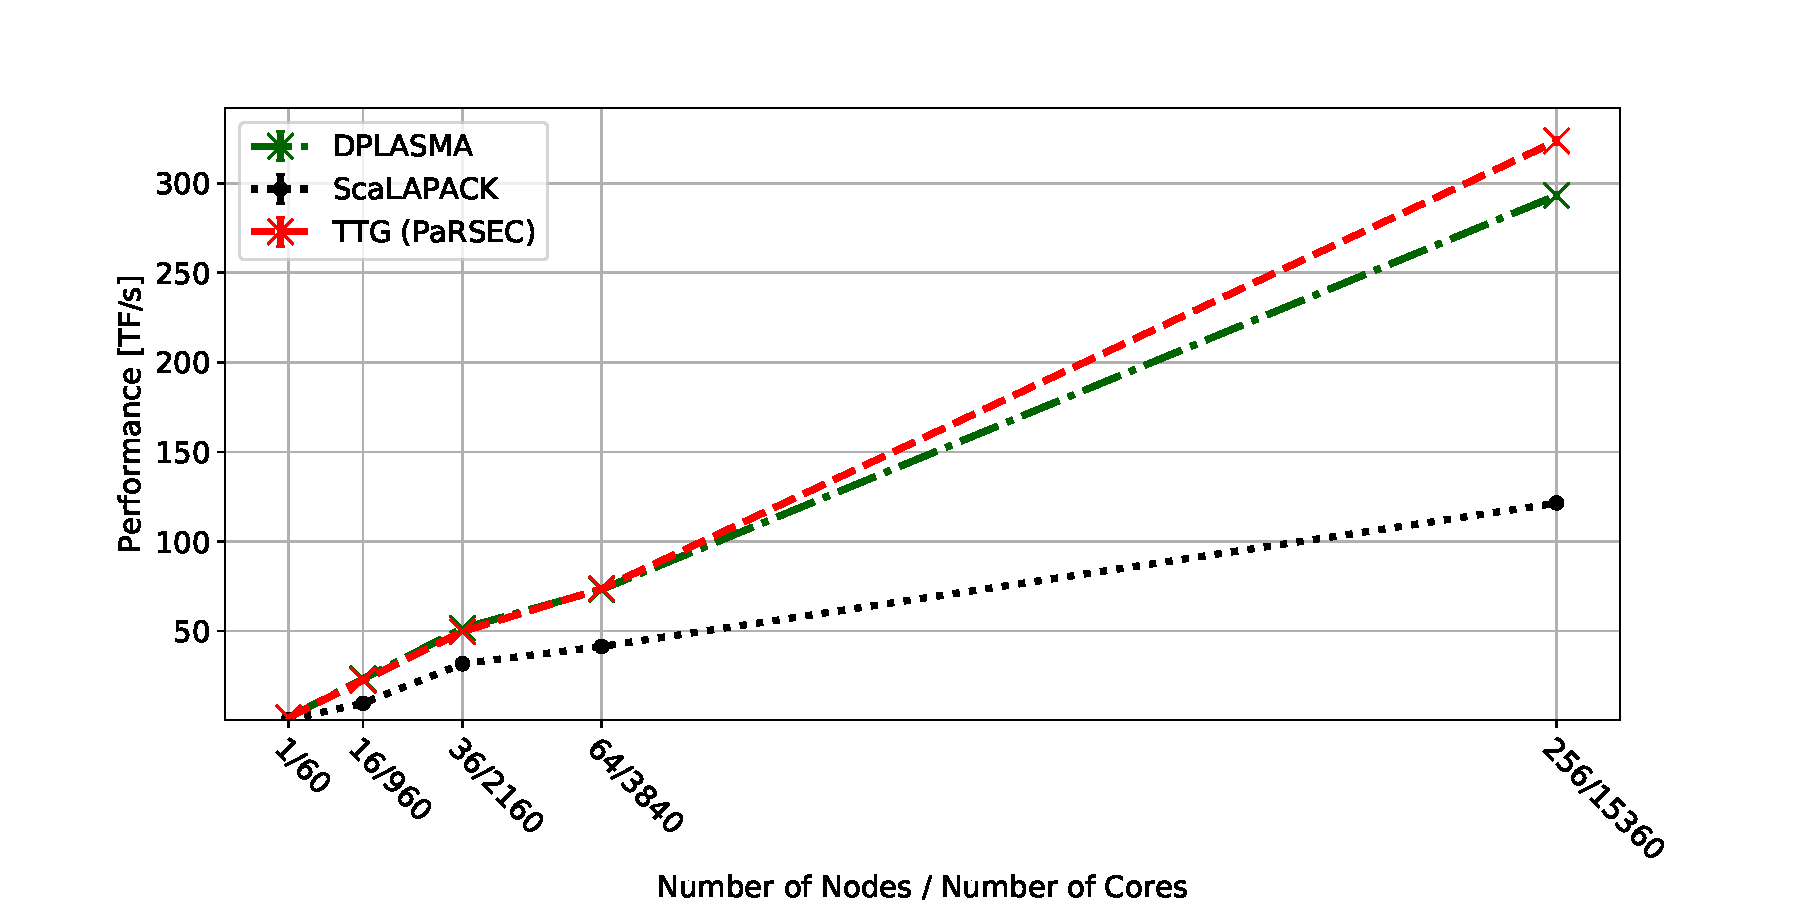
\includegraphics[width=.9\linewidth]{projects/2.3.1-PMR/2.3.1.09-ParSEC/dpotrf-ttg/dpotrf_1403612-page3.pdf}
\caption{Performance comparison between DPLASMA (PTG DSL), the TTG implementation, and ScaLAPACK, of the Cholesky factorization (double precision), for a fixed amount of memory per node (weak scaling).\label{fig:parsec:dpotrfttg:weakscale}}
\end{wrapfigure}
In the context of this collaboration, the PaRSEC team has provided
an efficient implementation of the TTG interface on top of the
PaRSEC runtime.
Figure~\ref{fig:parsec:dpotrfttg:weakscale} shows a performance
comparison on a 5,632 dual-socket 64-core AMD EPYC 7742 nodes equipped
with 256 GB main memory and connected through a Mellanox Infiniband
HDR 200 fabric, from 1 to 256 nodes (representing 15,360 cores in
total). We compare the TTG implementation of the dense Cholesky
factorization with the pdpotrf routines available in DPLASMA (thus
with the PTG implementation of the same algorithm), and in ScaLAPACK.
Each process holds a constant amount of memory, representing a
submatrix of $30k\times 30k$ elements. Each node runs 8 processes, and
each process is allocated 16 cores. With this weak-scaling experiment,
we observe that TTG behaves as efficiently and consistently as PTG. At
15,360 cores, the TTG implementation even goes slightly faster than
the PTG one, due to a better scheduling of the communications that are
discovered in a different order. Both task-based and PaRSEC-based
implementations go significantly faster than ScaLAPACK, which is the
expected behavior for a machine with so many cores per node.

%
% HIP / ROCM
%
\paragraph{Deployment on Early Access Systems\label{sec:parsec_early_access}}

The PaRSEC runtime as well as its dependent applications can compile and 
execute on the Spock early access system (EAS). Recent updates have identified
the root cause of prior difficulties with using atomic operations with the 
default compiler (LLVM-clang-13), which can now be safely used. The GNU compilers had been validated to be correct since last march.
%
The PaRSEC runtime can take advantage of the MI100 AMD accelerators (it uses the ROCM
software package to orchestrate host-device data transfer), and applications
using PaRSEC (e.g., DPLASMA dense linear algebra package, Massively Parallel Quantum Chemistry MPQC) have been modified to use rocsolver/rocblas
kernels. The performance of some of the kernels provided from rocsolver/rocblas 
has been found to be underperforming compared to theoretical peak, notably some
of the one-sided factorization in rocsolver. Despite these early system limitations, the PaRSEC
runtime is able to achieve a large proportion of peak performance on AMD
accelerated nodes. In addition to single-accelerator support, we validated the
multi-GPU scalability of PaRSEC on the DGEMM operation (dense matrix-matrix multiply),
where we have witnessed that the PaRSEC
version operates at the same rate as the rocblas DGEMM (as expected), and 
scales almost perfectly up to 4 GPUs. Similarly, the DPOTRF operation (LLT Cholesky factorization)
also shows very good multi-GPU scaling, and PaRSEC outperforms by
several order of magnitudes the performance of the rocsolver kernel. Performance of
the LLT factorization has also been verified to scale to multiple nodes. Looking at a
more challenging application pattern, we ran the irregular tensor contraction operation
from the MPQC chemistry ECP application. On this application, we showed a
very high rate of execution on multiple GPU accelerators, even when the sparsity
pattern of the data is high.

\begin{figure}
\centering
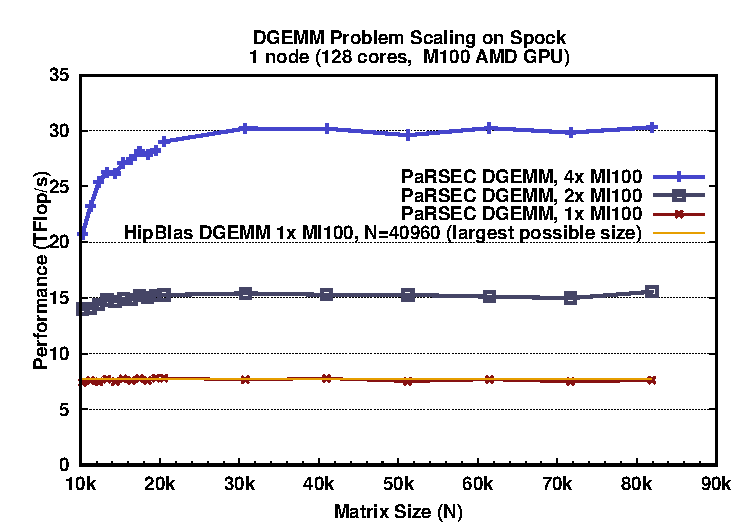
\includegraphics[width=.45\linewidth]{projects/2.3.1-PMR/2.3.1.09-ParSEC/spock-gemm-pbscal1.pdf}
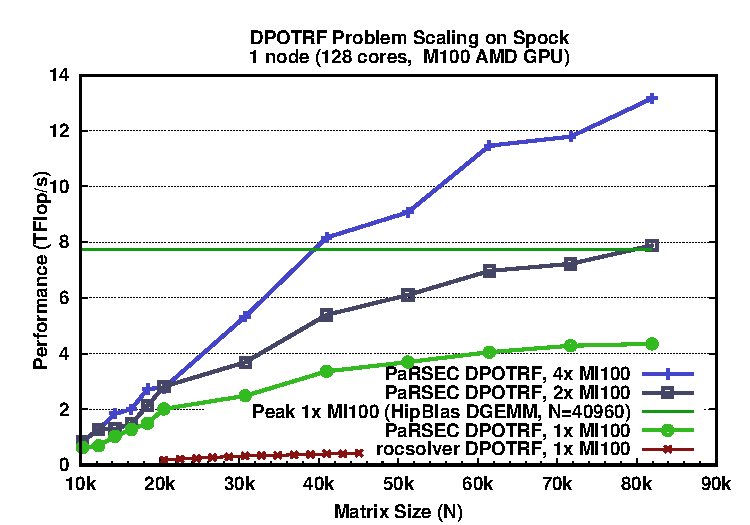
\includegraphics[width=.45\linewidth]{projects/2.3.1-PMR/2.3.1.09-ParSEC/spock-po-pbscal1.pdf}
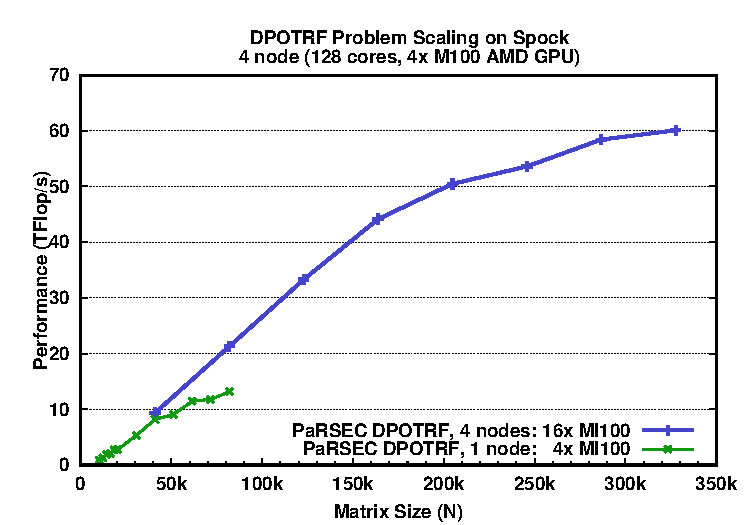
\includegraphics[width=.45\linewidth]{projects/2.3.1-PMR/2.3.1.09-ParSEC/spock-po-pbscal4.pdf}
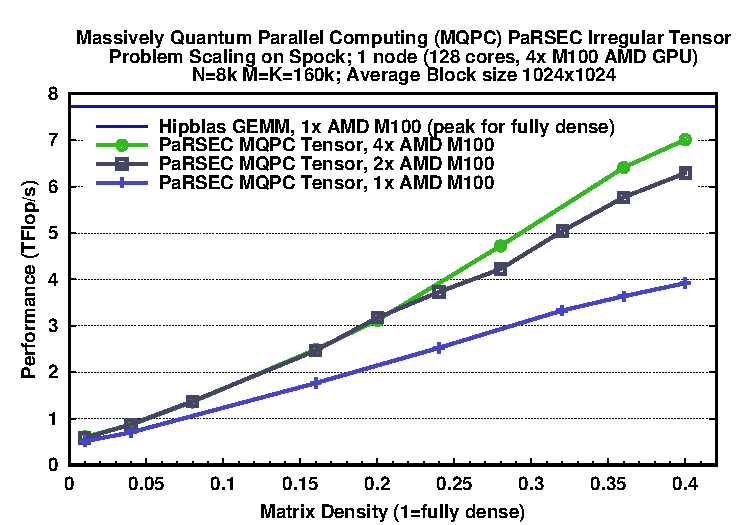
\includegraphics[width=.45\linewidth]{projects/2.3.1-PMR/2.3.1.09-ParSEC/spock-mqpc-density1.pdf}
\caption{Performance of PaRSEC on AMD accelerated system OLCF Spock.\label{fig:parsec:spock}}
\end{figure}

%Porting to Crusher has started in recent weeks.
The general software environment on Crusher being very similar to Spock, compiling PaRSEC
on Crusher required only minor adaptation of the build scripts (so as to find
and load the correct software dependencies from system-installed software).
PaRSEC has been verified to run on Crusher with basic correctness tests on up to 4 nodes, 
with multiple GPUs.

On both Crusher and Spock, we identified a limitation of the libSCI BLAS library:
it would not allow calling into BLAS operations from all cores when running one thread per-
core. This limitation has been communicated to the OLCF support team, but has not been
resolved thus far. Our mitigation strategy has been to compile our own copy of OpenBLAS as 
a substitute that can support enough threads to access the BLAS library.

We have also validated that PaRSEC deploys on Nvidia based DOE pre-exascale systems 
Perlmutter and Summit. All features of PaRSEC are supported on these machines, 
and performance has been validated to be consistent with expectations on a wide range
of applications.

Deployment on Intel Xe systems has been tested on the Yarrow system. We
also used Yarrow to develop an Xe specific device that manages host-device
memory movement. Deployment on the Arcticus EAS is ongoing. We verified that
the software can compile and are running basic tests with CPU workloads to verify
correctness.

\paragraph{Next Steps}
%\textit{Describe what you are working on next.}
% Improve DTE accelerator support and interoperability with other
% programming models
To provide programmers with more control over how accelerators are
integrated and used by the runtime, a need to provide finer control of the
resource usage by the runtime system has arisen. We are developing new APIs to
allow the programmers to advise the runtime system with respect to data
placement, prefetching, and management of cache.
%
Programming interoperability should not be limited to node-level programming
models but should extend to distributed programming. Execution modes where part
of the application is expressed in native MPI (including communicating tasks)
and other parts using PaRSEC DSLs, running above the task system in a tightly
coupled manner, are being developed.

% Facilitate DSL integration

% Provide better libraries and tools integration
The set of tools that come with the PaRSEC runtime environment to
assess performance, find bottlenecks, improve scheduling and debug the
task-based application are being improved to expose the information
in a format compatible with TAU, Score-P and other
tools that are already familiar to ECP users.

\newpage
\subsubsection{\stid{1.14} GASNet-EX}\label{subsubsect:gasnet-ex}
\paragraph{Overview} 

GASNet-EX~\cite{gasnet-site} is a portable high-performance communication layer
supporting multiple implementations of the Partitioned Global Address Space
(PGAS) model.
GASNet-EX clients include Pagoda's PGAS programming interface UPC++~\cite{upcxx-ipdps19,upcxx-site}
 and the Legion Programming
System~\cite{bauer2012legion,legion-site} (WBS~2.3.1.08).

GASNet-EX's low-overhead communication mechanisms are designed to maximize
injection rate and network utilization, tolerate latency through
overlap, streamline unpredictable communication events, minimize
synchronization,
leverage hardware support for communication involving accelerator memory,
and efficiently support small- to medium-sized
messages arising in ECP applications.  GASNet-EX enables the ECP
software stack to exploit the best-available communication mechanisms,
including novel features still under development by vendors.  The
GASNet-EX communications library and the PGAS models built upon it
offer a complementary, yet interoperable, approach to ``MPI + X'',
enabling developers to focus their effort on optimizing
performance-critical communication.

We are co-designing GASNet-EX with the UPC++ development team,
along with additional input from the Legion and
(non-ECP) Cray Chapel~\cite{chapel-chapter,chapel-site} projects.

\paragraph{Key Challenges}

Exascale systems will deliver exponential growth in on-chip parallelism and
reduced memory capacity per core, 
increasing the importance of strong
scaling and finer-grained communication events.  
Success at exascale demands minimizing software overheads,
especially avoiding long, branchy serial code paths; 
this motivates a requirement for efficient
fine-grained communication.
The pervasive use of accelerators introduces heterogeneous systems including
memory with properties that differ from host DRAM but can still benefit from
network offload support during communication.
These challenges are exacerbated by application trends; many of the ECP applications require
adaptive meshes, sparse matrices,
or dynamic load balancing.
All of these characteristics favor the use of
low-overhead communication mechanisms that
can maximize injection rate and network utilization, tolerate latency through
overlap, accommodate unpredictable communication events, minimize synchronization,
leverage hardware support for communication involving accelerator memory,
and efficiently support small- to medium-sized messages. The ECP software stack
needs to expose the best-available communication mechanisms, including novel
features being developed by the vendor community.

\paragraph{Solution Strategy}

The PGAS model is a powerful means of addressing these
challenges and is critical in building other ECP programming systems,
libraries, and applications.  We use the term {\em PGAS} for models that support
one-sided communication, 
including contiguous and non-contiguous remote memory access (RMA) operations such as put/get
and atomic updates. Some of these models also include support for remote function invocation.
GASNet-EX~\cite{gasnet-lcpc18} is a communications library that provides the foundation for implementing
PGAS models, and is the successor to the widely-deployed GASNet library.
We are building on nearly 20 years of experience with the GASNet~\cite{gasnet-site,gasnet-spec}
communication layer to provide production-quality implementations that include
improvements motivated by
technology trends and application experience.  

The goal of the GASNet-EX team is to provide a portable, high-performance PGAS
communication layer for exascale and pre-exascale systems, addressing the challenges
identified above.
GASNet-EX provides interfaces that efficiently match the RDMA capabilities of modern
inter-node network hardware and intra-node communication between distinct address spaces.
New interfaces for atomics and collectives have enabled offload to current
and future network hardware with corresponding capabilities.
New interfaces for non-host memory are designed to enable efficient transfers
to and from device memories, by leveraging such vendor technologies as
GPUDirect RDMA (GDR).
Together these design choices and their implementations supply the low-overhead communication
mechanisms required to address the requirements of exascale applications.

\begin{figure}[htb]
  \centering
  \subfloat[8-byte RMA Latencies\label{fig:rma-lat-bars}]{
     \includegraphics[width=0.432\textwidth]{projects/2.3.1-PMR/2.3.1.14-UPCxx-GASNet/latency_bars.pdf}
  }
  \subfloat[Summit Flood Bandwidth\label{fig:summit-bw}]{
     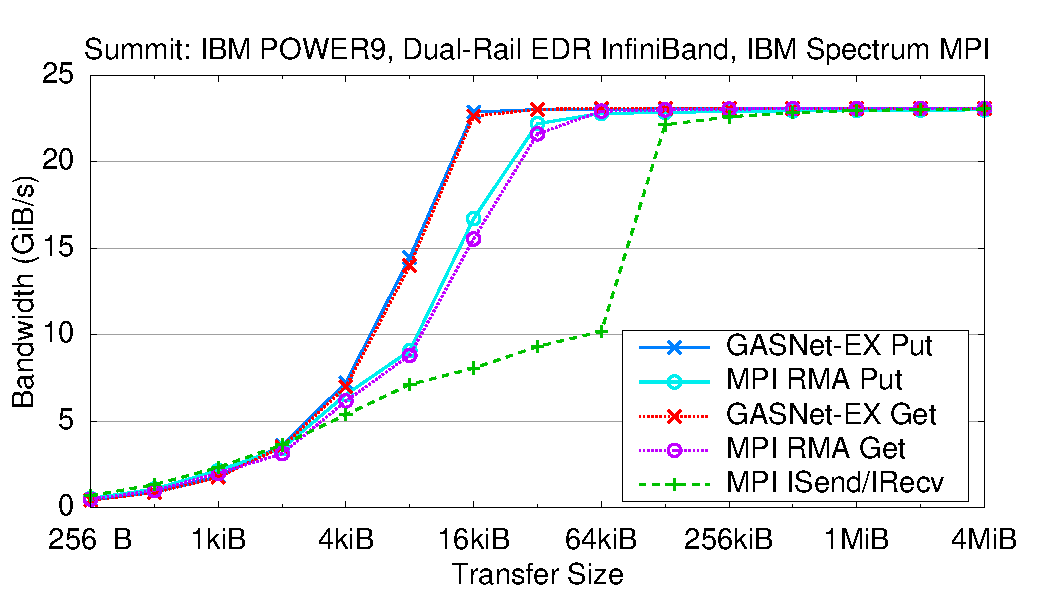
\includegraphics[width=0.504\textwidth]{projects/2.3.1-PMR/2.3.1.14-UPCxx-GASNet/Summit-slide-BW.pdf}
  }
  \caption{\label{fig:gasnet-ex-rma} Selected GASNet-EX vs. MPI RMA Performance Results}
\end{figure}

Figure~\ref{fig:gasnet-ex-rma} shows representative results from a
paper~\cite{gasnet-lcpc18} comparing
the RMA performance of GASNet-EX against MPI on multiple systems including
NERSC's Cori and OLCF's Summit%
\footnote{The paper's results from Summitdev
have been replaced by more recent (June 2019) results from OLCF's newer Summit system.}.
These results demonstrate the ability of a PGAS-centric runtime to
deliver performance as good as MPI, and often better.
%
The paper presents experimental methodology and system descriptions, which are
also available online~\cite{gasnet-site}, along with results for additional
systems.

Figure~\ref{fig:rma-lat-bars} shows the latency of 8-byte RMA Put and Get operations on
four systems, including two distinct network types and three distinct MPI
implementations.
%
GASNet-EX's latency is 6\% to 55\% better than MPI's on Put and 5\% to 45\%
better on Get.
%
Algorithms sensitive to small-transfer latency may become practical in PGAS
programming models due to these improvements relative to MPI.
%
Figure~\ref{fig:summit-bw} shows flood bandwidth of RMA Put and Get measured
on OLCF's Summit.
GASNet-EX's bandwidth is seen to rise to saturation at smaller
transfer sizes than IBM Spectrum MPI, with the most pronounced differences
appearing between 4KiB and 32KiB.
%
Comparison to the bandwidth of MPI message-passing (dashed green) illustrates the
benefits of one-sided communication, a major feature of PGAS models.


\paragraph{Recent Progress}

The most notable work on GASNet-EX in the past year has been in two areas:

\textbf{Device (GPU) Memory Support}.
``Memory kinds'' is the GASNet-EX term for support of communication involving
memory other than host memory.  In the context of ECP, the primary focus is
accelerator devices such GPUs.  However, the design is extensible to other
accelerators, such as FPGAs, and to storage.
Since late 2020, GASNet-EX has leveraged the GDR
capabilities of modern NVIDIA GPUs and Mellanox network adapters (such as those
on Summit) to perform one-sided RMA involving GPU memory without
the overheads of staging through intermediate buffers in host memory.
The GASNet-EX APIs for memory kinds have been co-designed with the developers
of UPC++ and the Realm runtime layer of the Legion Programming System
(WBS~2.3.1.08), and both projects have leveraged this support since
their respective late 2020 releases.
Performance of GASNet-EX memory kinds, including via Legion and UPC++
benchmarks, is featured on an SC21 research poster~\cite{gasnet-poster-sc21},
and additional UPC++ performance results using memory kinds appear in
Figure~\ref{fig:paw21_interop_strong_scaling} in
Section~\ref{subsubsect:upcxx}.
The most recent work on memory kinds has extended the implementation in two directions:
adding support for the UCX network API and for GPUs using the AMD HIP API.
The net result is support for four combinations of network API and GPU vendor.

\textbf{Tuning}.
We have devoted effort in the past year to improving the performance and memory
use of the GASNet-EX runtime.  Examples of this work include significant
improvements to InfiniBand support which (1) reduce memory consumption at large
job sizes and (2) improve scaling to large thread counts in multi-threaded
clients.  Other recent tuning efforts have reduced the overheads for put, get
and atomic updates in intra-node shared memory.

\paragraph{Next Steps}

Our next efforts include:

\textbf{Device (GPU) Memory Support}.
We will continue work in the area of GASNet-EX memory kinds, including the
hardening and tuning of the current implementation.
As access to relevant systems is secured, we plan to extend support to
additional accelerators and networks, with Intel GPUs and the HPE Slingshot
network being the most important examples for ECP.

\textbf{Client-Driven Tuning}.
In collaboration with authors of client runtimes using GASNet-EX (most notably
UPC++ and Legion) and their users (such as ExaBiome), we will continue to
identify and address any significant scalability issues or performance
anomalies which are discovered.

\clearpage

\subsubsection{\stid{1.14} UPC++} 
\paragraph{Overview} 
The UPC++ project~\cite{upcxx-site} at LBNL is developing a C++ library
that supports Partitioned Global Address Space (PGAS) programming~\cite{Bachan:paw17,upcxx-spec}.
The current ECP-funded version of
UPC++ is markedly different from an earlier prototype designated V0.1 \cite{zheng:ipdps14}.  
First, all communication is \emph{asynchronous}, to allow the overlap of computation and
communication, and to encourage programmers to avoid global synchronization. Second, all communication
is \emph{syntactically explicit}, to encourage programmers to consider the costs of communication. Third,
UPC++ encourages the use of \emph{scalable data-structures}
and avoids non-scalable library features.
%such as symmetric heaps. % this is too strong, inflammatory and not supported
All of these principles are intended to provide a programming model that can
scale efficiently to potentially millions of processors.
% We are revising the library under the auspices of the DOE's Exascale Computing
% Project, to meet the needs of applications requiring PGAS support.
UPC++ is well-suited for implementing elaborate distributed data structures where
communication is irregular or fine-grained. 
The UPC++ communication interfaces for Remote Memory Access (RMA) 
and Remote Procedure Calls (RPC)
are composable and fit naturally within the context of modern C++.

UPC++ is needed for ECP because it delivers low-overhead communication that runs
at close to hardware speeds, embracing 
interest by vendors in the PGAS model that
efficiently matches the RDMA mechanisms offered by
network hardware and on-chip communication between distinct address
spaces.  
Because ECP applications rely on irregular representations
to improve accuracy and conserve memory, the UPC++ library provides
an essential ingredient for the ECP software stack.  It enables
effective scaling of Exascale software by minimizing the work funneled
to lightweight cores, avoiding the overhead of long, branchy serial
code paths, and supporting efficient fine-grained communication.  The
importance of these properties is reinforced by application trends;
many ECP applications require the use of irregular data structures such as 
adaptive meshes, sparse
matrices, particles, or similar techniques, and also perform load balancing.  UPC++'s
low-overhead communication mechanisms can maximize injection rate and
network utilization, tolerate latency through overlap, streamline
unpredictable communication events, minimize synchronization, and
efficiently support small- to medium-sized messages arising in such
applications.  UPC++ enables the ECP software stack to exploit
the best-available communication mechanisms, including novel features
being developed by vendors.  This library offers a complementary,
yet interoperable, approach to MPI with OpenMP, enabling developers to
focus their effort on optimizing performance-critical communication.

\paragraph{Key  Challenges}

As a result of technological trends, the cost of data motion is steadily increasing relative to that of computation.  To reduce communication costs we need to 
reduce the software overheads and hide communication latency behind available computation. UPC++ addresses both strategies.
To reduce software overheads, UPC++ takes advantage of the GASNet-EX~\cite{gasnet-lcpc18,gasnet-site}
communication library's 
low-overhead communication as well as access to any special hardware
(see Section~\ref{subsubsect:gasnet-ex} on GASNet-EX, which is being co-designed).
UPC++ supports asynchronous communication via one-sided RMA and RPC.


% A challenge in the ECP-ST effort is to maintain interoperability among run times,
% that invoke the back end to carry out communication. The difficulty is that each
% backend operates under the assumption that it "owns" the network.
% But many ECP applications employ (or will under ECP) multiple runtimes;
% thus interoperability is of paramount concern.
% Our approach is conservative; so long as entries and exits between different
% models is sufficiently coarse grained, then it is feasible to synchronize
% at a barrier at each transition.

\paragraph{Solution Strategy}

The UPC++ project has two primary thrusts:
\begin{enumerate}
\item \textbf{Increased performance through reduced communication costs:} The
UPC++ programmer can expect communication to run at close to hardware speeds.
Asynchronous execution enables an application to hide communication behind
available computation.

\item \textbf{Improved productivity:}  UPC++'s treatment of asynchronous
execution relies on futures and promises, and these simplify the management of
asynchrony.

\end{enumerate}

The PGAS one-sided RMA communication employed by UPC++
benefits application  performance by mapping tightly onto the RDMA mechanisms
supported by the network hardware. GASNet-EX provides the
thin middleware
needed to enable this model to run at close to hardware speeds, across platforms ranging from laptops to supercomputers.
One-sided communication also has another benefit:
it decouples synchronization from data motion,
avoiding the fine-grained synchronization overheads of two-sided message-passing.

UPC++'s Remote Procedure Call (RPC)
%, which is built on GASNet Active Messages,
% provides additional control over asynchronous execution, by enabling
enables the programmer
to execute procedure calls on remote processors.
RPC is useful in managing access to complicated irregular data structures,
and in expressing asynchronous task execution, where communication patterns
are data-dependent and hence difficult to predict.

%UPC++ addresses productivity via one-sided data motion, remote procedure calls,
%and future-based management of asynchrony.
%Futures enable the programmer
%to capture data readiness state,
%which is useful in making scheduling decisions,
%and to attach handlers that 
%execute asynchronously as dependencies become
%satisfied. Futures may also be conjoined, to aggregate
%completion processing. The outcome is to avoid explicit synchronization of completion at a fine granularity.

As one example of how our approach is applicable to real problems
we have implemented a distributed hash table, which serves as a proxy
for a key phase in the HipMer application of the Exabiome Project (WBS~2.2.4.04).
This implementation scales efficiently
to a large number of processors. RPC was observed to simplify the implementation
considerably, by avoiding data hazards without the need for locking.
Figure~\ref{fig:dht} illustrates the benefits of the UPC++ model 
in a weak scaling study up to 34,816 processes on the KNL partition of NERSC's Cori.


\begin{figure}[htb]
\centering
      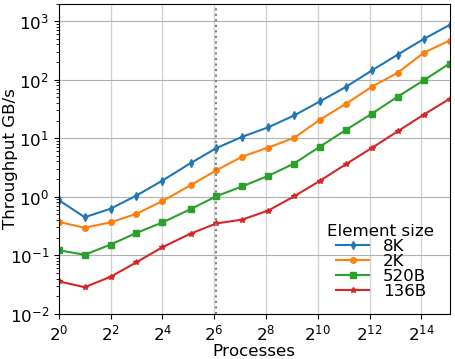
\includegraphics[scale=0.75]{projects/2.3.1-PMR/2.3.1.14-UPCxx-GASNet/all-cori-knl-out-inserts-wait.png}
  \caption{Weak scaling of distributed hash table insertion on the KNL partition of NERSC's Cori platform. The dotted line represents the processes in one node.}
  \label{fig:dht}
\end{figure}



\paragraph{Recent Progress}

\begin{enumerate}
\item \textbf{Memory Kinds.}
Unified abstractions for 
transferring data back and forth between device (e.g. GPU) and host memory, possibly remote.
By unifying the means of expressing data transfer among the collective memories of a heterogeneous system with different memory kinds,
the abstractions enable ECP applications to utilize accelerators, which are necessary to attain peak performance on ECP platforms.
The design and abstraction enables eventual hardware offload (such as to GPUDirect) of device data transfers, support for which will be provided in the near future by GASNet-EX.

\item \textbf{Portability and Sustainability.}
%Ensure that UPC++ remains viable as new compiler versions are released into the ECP software stack. 
UPC++ benefits to productivity rely heavily on template meta-programming, using features added in C++11.
However not all relevant C++ compilers comply sufficiently with the C++11 standard, 
necessitating deployment of various work-arounds within the UPC++ implementation.
The past year has seen the addition of UPC++ support for seven new CPU/compiler pairs.
A UPC++ Spack package has also been added to the E4S PMR SDK (Section~\ref{subsubsect:e4s}).

\end{enumerate}

\paragraph{Next Steps}

\begin{enumerate}
\item \textbf{Performance.}
With the help of our stakeholders, we are identifying portions of the UPC++
implementation where performance tuning is most needed and/or beneficial.
A recent example is deployment of an optimized implementation for
RMA puts using target-side completion notification.

\item \textbf{Productivity.}
With the core API specification and implementation of UPC++ nearly complete, we
are shifting focus toward some productivity-oriented features.  These include
UPC++ serialization of non-trivial user types and a distributed array facility
for UPC++.

\item \textbf{Outreach.}
We have begun activities designed to strengthen collaboration with our
stakeholders (both current ones, and potential future ones).  This includes
holding training events for users of UPC++ and circulating working group
drafts of productivity features (above) to solicit feedback.

\end{enumerate}

\newpage
\subsubsection{\stid{1.16} SICM}
\paragraph{Overview} The goal of this project is to create a universal interface for discovering, managing and sharing within complex memory hierarchies. The result will be a memory API and a software library which implements it. These will allow operating system, runtime and application developers and vendors to access emerging memory technologies. The impact of the project will be immediate and potentially wide reaching, as developers in all areas are struggling to add support for the new memory technologies, each of which offers their own programming interface. The problem we are addressing is how to program the deluge of existing and emerging complex memory technologies on HPC systems. This includes the MCDRAM (on Intel Knights Landing), NV-DIMM, PCI-E NVM, SATA NVM, 3D stacked memory, PCM, memristor, and 3Dxpoint. Also, near node technologies, such as PCI-switch accessible memory or network attached memories, have been proposed in exascale memory designs. Current practice depends on ad hoc solutions rather than a uniform API that provides the needed specificity and portability. This approach is already insufficient and future memory technologies will only exacerbate the problem by adding additional proprietary APIs. Our solution is to provide a unified two-tier node-level complex memory API. The target for the low-level interface are system and runtime developers, as well as expert application developers that prefer full control of what memory types the application is using. The high-level interface is designed for application developers who would rather define coarser-level constraints on the types of memories the application needs and leave out the details of the memory management. The low-level interface is primarily an engineering and implementation project. The solution it provides is urgently needed by the HPC community; as developers work independently to support these novel memory technologies, time and effort is wasted on redundant solutions and overlapping implementations. Adoption of the software is focused on adsorption into existing open source projects such as hwloc, Umpire, CLANG/LLVM, OpenMP, and Jemalloc.
\begin{itemize}
\item  Low-Level Interface: Finished refactor of low-level interface supporting memory arenas on different memory types. Added initial support for Umpire, OpenMP. Reviewing features need to fully support these runtimes. SICM now supports Intel Optane memory, the first NVM memory that can be used as an extension of traditional DRAM memory.
Pull requests have been developed for OpenMP/CLANG/LLVM and Umpire. the patches to Clang/LLVM/OpenMP turn OpenMP memory spaces in OpenMP 5.x into SICM library calls in the LLVM/OpenMP runtime. The same codepath that supports memkind library was refactored to support multiple custom memory allocators – more general than just SICM support.
SICM currently supports ``pragma openmp allocate'' with  memory types: omp\_ (default, large\_cap, const, high\_bw, low\_lat ) \_mem\_spaces and supports KNL, Optane, testing on Sierra/Summit.
\item  High-Level Graph Interface: Metall is a persistent memory allocator designed to provide developers with an API to allocate custom C++ data structures in both block-storage and byte- addressable persistent memories (e.g., NVMe and Intel Optane DC Persistent Memory) beyond a single process lifetime. Metall relies on a file-backed mmap mechanism to map a file in a filesystem into the virtual memory of an application, allowing the application to access the mapped region as if it were regular memory which can be larger than the physical main-memory of the system.
\item Analysis: 
SICM has employed application profiling and analysis to direct data management across complex memory hierarchy, the team extended the SICM high-level interface with application-directed data tiering based on the MemBrain approach which is more effective than an unguided first touch policy.  The impact of using different data features to steer hot program data into capacity-constrained device tiers was modeled.
\end{itemize}
\paragraph{Next Steps}
\begin{itemize}
\item  Low-Level Interface: Focus on performance of support for runtimes and adding feature requested to support Umpire, OpenMP and MPI and address the slow move pages implementation in the Linux kernel – (collaboration with RIKEN). Test with proxy applications for functionality and correctness. Investigate Linux kernel modifications for page migration in collaboration with ECP project Argo 2.3.5.05 and RIKEN research center in Japan, on-going. Start collaborating with applications to enable use of heterogenous memory on ECP target platforms. Additionally, the team needs to finalize the memory topology discover with the hwloc team.
\item For the analysis work the team will extend and harden the tools for guiding application memory management and investigate feature categories to classify objects associated with different features such as size, type, allocation time, etc to guide data placement.
\item For the Metall high-level interface we plan to continue outreach to ExaGraph to store graph data as well as other intermediate data into PM leveraging Metall. We also plan to support UMap (user-level mmap library in Argo PowerSteering project) underneath Metall to enhance its performance and capability.
\end{itemize}



\newpage
\subsubsection{\stid{1.17} Open~MPI for Exascale (OMPI-X)}\label{subsubsect:openmpi}

%% {\itshape

%% 	\begin{enumerate}
%% 	\item Rename this file to your project WBS-projectname.tex, for example 2.3.3.01-XSDK4ECP.tex.
%% 	\item Complete this template for your project.  Limit your text to two pages, not counting citations.
%% 	\item Please avoid changing the content of main.tex.
%% 	\item Put any references in a .bib file with the same root name, for example 2.3.3.01-XSDK4ECP.bib.
%% 	\item Remember to include any image files you reference in your text.
%%     \item The files 2.3.3.01-XSDK4ECP.tex, 2.3.3.01-XSDK4ECP.bib and xSDK-diagram.jpeg are included as examples for your reference.  You can remove them from what you upload.
%% 	\end{enumerate}
%% }

\paragraph{Overview}
%% \textit{Provide an overview of your project.  You might find that the introductory text from your Fall 2017 Project Summary \url{https://confluence.exascaleproject.org/display/1ST/Fall+2017+ECP+ST+Project+Summaries} useful as a starting draft.}

The OMPI-X project ensures that the Message Passing Interface (MPI)
standard, and its specific implementation in Open~MPI meet the needs
of the ECP community in terms of performance, scalability, and
capabilities or features. MPI is the predominant interface for
inter-process communication in high-end computing.  Nearly all of the
ECP application (AD) projects (93\%~\cite{Bernholdt:2018:SMU-tr})
and the majority of ST projects
(57\%~\cite{Bernholdt:2018:SMU-tr}) rely on it.
With the impending exascale era, the
pace of change and growing diversity of HPC architectures pose new
challenges that the MPI standard must address.  The OMPI-X project is
active in the MPI Forum standards organization, and works within it to
raise and resolve key issues facing ECP applications and libraries.

Open~MPI is an open source, community-based implementation of the MPI
standard that is used by a number of prominent
HPC vendors as the basis for their commercial MPI offerings.   The
OMPI-X team is comprised of active members of the Open~MPI community,
with an extensive history of contributions to this community.
The OMPI-X project focuses on prototyping
and demonstrating exascale-relevant proposals under consideration by
the MPI Forum, as well as improving the fundamental performance and
scalability of Open~MPI, particularly for exascale-relevant platforms
and job sizes.
MPI users will be able to take advantage of these
enhancements simply by linking against recent builds of the Open~MPI
library.

In addition to MPI and Open~MPI, the project also includes two other products,
which are less visible to the end user, but no less important.
PMIx (Process Management Interface for Exascale) provides facilities for
scalable application launch, process wire-up, resilience, and coordination between runtimes.
It originated as a spin-off from the Open~MPI community, but is now developing a
community of its own as adoption grows.  Starting in FY20,
Qthreads (formerly WBS 2.3.1.15) is also part of the OMPI-X project.  Qthreads is a
user-level lightweight asynchronous thread library particularly focused on improving support for
multithreading in the context of network communications.  Both PMIx and Qthreads help the
OMPI-X project address key issues of performance and capability for exascale applications.


\paragraph{Key  Challenges}
%% \textit{Describe what is hard to do, why it is challenging.}
A number of aspects of exascale levels
of computing pose serious challenges to the tried and true message
passing model presented by MPI and its implementations, including Open~MPI.
%
Keeping pace with changes in HPC architecture is a major challenge.
Examples include massive node-level concurrency, driving the
growth of MPI+X programming approaches,
and the complex memory architectures, which make the placement of data
within memory more important. In the near-term, with GPUs dominating the exascale
environment, how code running on the GPUs interacts with MPI and inter-process
communications must also be addressed.  This will require both changes to the standard
and changes and improvements within implementations.
%
Performance and scalability become both more important and more
challenging as node counts increase
and memory per MPI rank trends downward.
%
Finally, as we identify solutions to these challenges that must be
implemented within the MPI \emph{standard} rather than particular MPI libraries,
we must work within the much larger and broader MPI
community that may not always be attuned to the needs of computing at the largest scales.

\paragraph{Solution Strategy}
%% \textit{Describe your basic strategy for addressing the challenges.}
The OMPI-X project is working across a number of fronts to address
these challenges.

\subparagraph{Runtime Interoperability for MPI+X and Beyond} MPI is
increasingly being used concurrently with other runtime environments.
This includes both MPI+X approaches, where X
is most often a threading model, such as OpenMP, as
well as the use of multiple inter-process runtimes within a single
application.  Concerns include awareness of other runtimes,
cooperative resource management capabilities, and ensuring that all
concurrently active runtimes make progress.  We are developing APIs and
demonstrating capabilities for interoperability in both MPI+X and
multiple inter-process runtime situations.

\subparagraph{Extending the MPI Standard to Better Support Exascale
Architectures} The MPI community is standardizing a
number of ideas that
are particularly important to supporting
the architectural and system size characteristics anticipated for
exascale.  Partitioned communications (previously called \textit{Finepoints})
deal with the growing use of threading for node-level concurrency, in
combination with MPI.  Sessions increases the flexibility of MPI
semantics in a number of areas, which in turn can open opportunities
for enhanced scalability, as well as easier support for
multicomponent applications such as coupled multiphysics
simulations. Error management and recovery capabilities are key to
ensuring that applications can detect and respond effectively when errors,
inevitably, occur during execution.  We are helping to drive incorporation
of these and other ideas into the MPI standard by developing prototypes and
working with ECP teams and the broader community to demonstrate their
feasibility and value.

\subparagraph{Open~MPI Scalability and Performance} As we push the scale of
both hardware and applications, we stress MPI implementations and
expose areas that need to be improved.
OMPI-X is targeting key components within Open~MPI, such as threading capabilities,
memory usage, remote memory access (RMA), tag matching, and other areas,
for improvements in both scalability and performance.

\subparagraph{Supporting More Dynamic Execution Environments} We are
developing and implementing strategies to help MPI applications
better deal with topological process layout preferences
and contention in the network.

\subparagraph{Resilience in MPI and Open~MPI} Concerns about system and
application resilience increase as either scales in size.  Our goal in
this area is to ensure that MPI, Open~MPI, and PMIx provide not only
support for simplified
recovery for the widely used checkpoint/restart fault tolerance strategy, but also the building
blocks to support more general error management and recovery by applications (the evolution of the User-Level
Fault Mitigation concept). We work within the MPI Forum, implement,
and train users on resilience strategies.

\subparagraph{MPI Tools Interfaces}  Several interfaces within the
MPI standard are primarily used to support performance and
correctness tools.
The MPI Forum is in the process
of making significant revisions and extensions to these interfaces.
We will track the discussions in the Forum and provide prototype
implementations within Open~MPI to facilitate evaluation and provide
feedback.
We will work with the
ECP community, including tool developers, to make additional data
available through the MPI\_T interface.

\subparagraph{Quality Assurance for Open~MPI}  We are enhancing the
Open~MPI testing infrastructure, adding tests to reflect ECP
requirements, and instantiating routine testing on systems of
importance to ECP, both for correctness and performance.

\begin{wrapfigure}{r}{0.40\textwidth}
    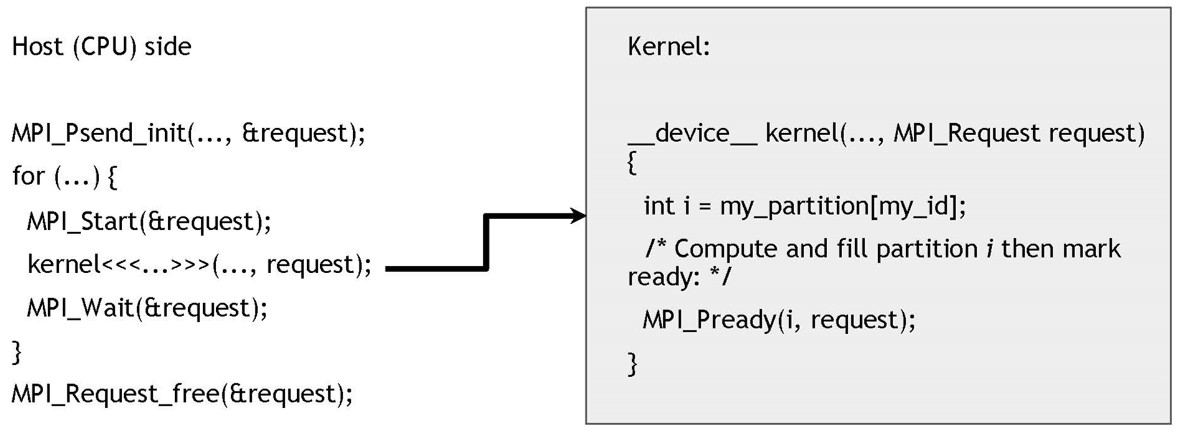
\includegraphics[width=0.40\textwidth]{projects/2.3.1-PMR/2.3.1.17-OMPI-X/partitioned-comms-code.jpg}
    \caption{Schematic code illustrating use of partitioned communications from a GPU kernel.  
    Host code (left) sets up communication, GPU kernel (right) triggers send (MPI\_Pready).}
    \label{fig:partitioned-communications}
\end{wrapfigure}

\paragraph{Recent Progress}
%% \textit{Describe what you have done recently.  It would be good to
%% have some kind of figure or diagram in this section.}
The MPI Forum finalized and released version 4.0 of the standard in June 2021.  The OMPI-X team helped drive
the incorporation a number of new features and capabilities considered important for exascale applications.
These include sessions and a number of error management and recovery features
based on the long-standing User-Level Fault Mitigation (ULFM) concept.  Partitioned communications (Figure~\ref{fig:partitioned-communications})
is another major addition to the standard which is designed to benefit massively-threaded environments, such as GPU accelerators, by supporting
incremental completion of the communication as portions of the buffer become ready.
These capabilities have at least prototype-level implementations available in the Open~MPI library, allowing interested project teams to start
exploring the new capabilities.  

As the MPI Forum continues its work beyond 4.0, the OMPI-X team continues 
its strategic involvement on topics that did not make the 4.0 release of the standard or further enhancements to 4.0 features
to improve support for high-end systems and the ECP community,  particularly in the context of resilience. The ULFM
proposal has been updated to reflect those features that have been incorporated into 4.0, as well as the discussions
within the Forum.  For the complementary Reinit simplified checkpoint/restart proposal (Figure~\ref{fig:reinit}), we have carried out a formal verification on the recovery algorithm. 
This ensures that the protocol, which we plan to propose for a future version of MPI, correctly handles the recovery phase 
of a failure response, including correct propagation of notifications, absence of deadlocks, and proper termination.
During the past year, the Reinit recovery protocol has been formally verified
and a prototype implementation has been developed in Open~MPI.  Performance evaluation
of the approach show it offering superior performance to traditional checkpoint/restart
for the HPCG benchmark against different types of failures (Fig.~\ref{fig:reinit}).

\begin{figure}
    \centering
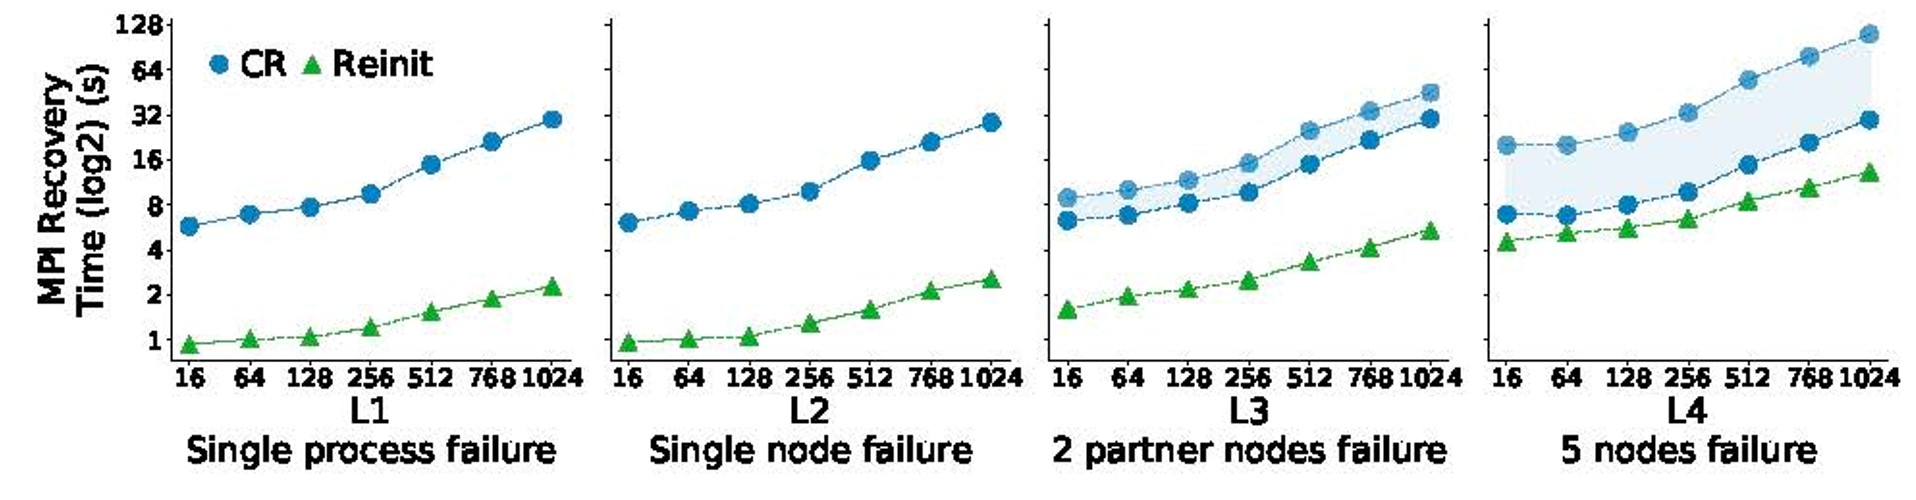
\includegraphics[width=0.80\textwidth]{projects/2.3.1-PMR/2.3.1.17-OMPI-X/reinit-performance.jpg}
\caption{Comparison of recovery times for traditional checkpoint/restart (blue) and Reinit (green) for the HPCG benchmark.  
Each graph represents different types/severities of failures.}
\label{fig:reinit}
\end{figure}

As part of the larger Open~MPI community, we are working towards a major-version
release (v5.0.0), planned for late CY2021.  This release will include many contributions
of the OMPI-X team, including the beginnings of our work towards full support for
MPI 4.0, user-level fault mitigation and FP16 support (both of which we will be advocating
for future MPI standards), and performance enhancements such as SIMD support for MPI reductions,
and improvements to collective and atomic operations.

\begin{wrapfigure}{r}{0.40\textwidth}
    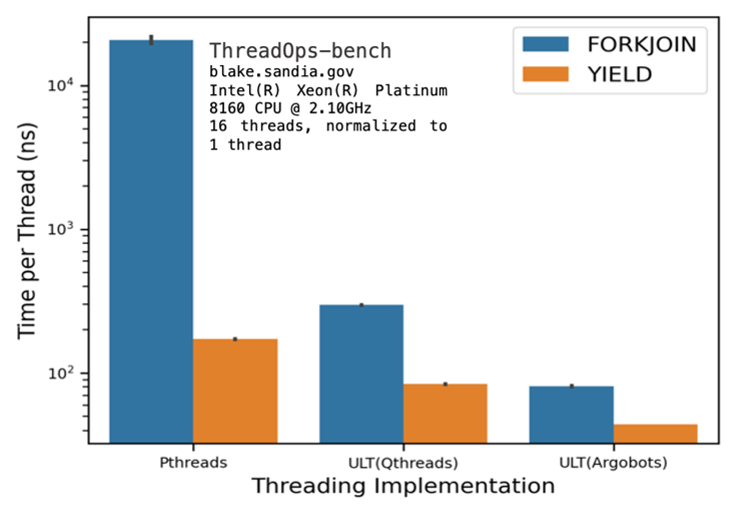
\includegraphics[width=0.40\textwidth]{projects/2.3.1-PMR/2.3.1.17-OMPI-X/ult-performance.png}
    \caption{Illustration of relative costs of PThreads vs ULT threads (Qthreads, Argobots) using ThreadOps benchmark for fork-join and yield operations.}
    \label{fig:ult-performance}
\end{wrapfigure}

To support highly-threaded MPI+X use cases primarily on the CPU side, the OMPI-X project has teamed with the MPICH and Argobots ECP teams (WBS 2.3.1.07 and 2.3.2.11)
to define interfaces in both MPICH and Open~MPI to support the use of lightweight user-level threading (ULT) libraries such as Qthreads or BOLT
as an alternative to Pthreads.  The new ULT support, now integrated into both libraries, offer significantly improved performance compared to 
the traditional Pthreads implementation (Figure~\ref{fig:ult-performance}).

Another key product that the OMPI-X project supports is the Process Management Interface for Exascale (PMIx).  PMIx includes both a community standard
and a reference implementation, OpenMPIx.  Open~MPI relies on the PMIx standard and the PRRTE reference runtime for process startup, wireup, and runtime coordination.
It is also used and implemented by a variety of other libraries and projects, including LLNL's Flux resource manager (WBS 2.3.6.02), which is in turn part of the ExaWorks toolkit (WBS 2.3.5.10).
During the past year, version 4.0 of the PMIx standard was released, as well as version 4.1.0 of OpenPMIx and version 2.0.0 of PRRTE.

In addition to these activities, we continue to support quality assurance of the Open~MPI code base through more and better testing.  The Open~MPI testing infrastructure, 
MTT, continues to be improved for flexibility and capability.  One of this year's noteworthy efforts was the addition of the bueno application test harness to the testing 
system.  The facilitates incorporating third-party test cases (i.e. based on user applications) into the routine testing process without having to commit them to the
Open~MPI testing repository.  We are also working to establish more frequent testing regimes on key DOE hardware platforms.

\paragraph{Next Steps}
%% \textit{Describe what you are working on next.}
The delivery of the first HPE Slingshot-11 (SS-11) network, as part of the Frontier system, at the beginning of FY22 finally affords us
the opportunity to start our work to ensure that Open~MPI provides good support for SS-11, which we expect to be the focus of significant
effort this year.  SS-11 will be used on both Frontier and Aurora, so much of the work will support both systems, though there will be differences 
in on-node (particularly GPU-to-GPU) transfers due to the different GPU accelerators.  The different workload management solutions on the two platforms
will also need to be supported.  Additionally, we will be in a much better position to work with application teams who can benefit from the new capabilities 
embodied in MPI 4.0, but who have been reluctant to adopt them until they were officially part of the standard.  
We will likewise continue to identify and improve performance and scalability bottlenecks and drive forward on
the core themes outlined in our Solution Strategy.

\paragraph{Early Access System Experience}
Most of the early access systems have utilized InfiniBand interconnects, which are well-supported 
by Open MPI (the HPE Slingshot-10 interconnect is also InfiniBand).  The Frontier test and development
system Crusher was the first system available with the new Slingshot-11 network.  A subset of the
OMPI-X team obtained access to Crusher in December, and have been working to port Open MPI to
the SS-11 interconnect.  The basic approaches available leverage either Open Fabric providers or
the UCX communication infrastructure, or some combination.
So far, we have confirmed basic point-to-point functionality using the HPE-provided
CXI Open Fabric provider, and partial intra-node shared memory functionality through the 
UCX communications framework.
We plan to continue exploring all three paths until we arrive at a solution that provides full functionality
with the expected performance.

The Qthreads user-level lightweight threading package is not dependent on the network, nor on the GPUs
so it is easier to port.  It has been confirmed to work on Spock (the Frontier early access system).
Challenges getting the Qthreads team access to ANL early access systems have delayed demonstration
of the functionality there, but we do not anticipate any problems.  The team just recently obtained
access to Arcticus and plans to test Qthreads there shortly.

\newpage
%  The RAJA text is out-of-date.  Need to comment it out.
%
%\subsubsection{\stid{1.18} ISC4MCM (RAJA)} 
%
%\paragraph{Overview.} 
%The Integrated Software Components for Managing Computation and Memory 
%Interplay at Exascale (ISC4MCM) project is providing software libraries that 
%enable application and library developers to meet advanced architecture 
%portability challenges. The project goals are to enable writing performance 
%portable computational kernels and coordinate complex heterogeneous memory 
%resources among components in a large integrated application. These 
%libraries enhance developer productivity by insulating them from much of the 
%complexity associated with parallel programming model usage and 
%system-specific memory concerns.
%
%The software products provided by this project are three complementary and 
%interoperable libraries:
%\begin{enumerate}
%\item {\bf RAJA:} Software abstractions that enable C++ developers to write
%  performance portable (i.e., single-source) numerical kernels (loops). 
%\item {\bf CHAI:} C++ ``managed array'' abstractions that enable transparent
%  and automatic copying of application data to execution memory spaces at run
%    time as needed based on RAJA execution contexts.
%\item {\bf Umpire:} A portable memory resource management library that provides
%  a unified high-level API for resource discovery, memory provisioning,
%    allocation, access, operations, and introspection.
%\end{enumerate}
%
%Capabilities delivered by these software efforts are needed to manage the
%diversity and uncertainty associated with current and future HPC architecture
%design and software support. Moving forward, ECP applications and libraries 
%need to achieve performance portability: without becoming bound to particular
%(potentially-limiting) hardware or software technologies, by insulating 
%numerical algorithms from platform-specific data and execution concerns, and 
%without major disruption as new machine, programming models, and vendor
%software become available.
%
%These libraries in development in this project are currently used in production
%ASC applications at Lawrence Livermore National Laboratory (LLNL). They are
%also being used or being explored/adopted by several ECP application and
%library projects, including: LLNL ATDM application, GEOS (Subsurface), SW4
%(EQSIM), MFEM (CEED co-design), and SUNDIALS.
%
%The software projects are highly-leveraged with other efforts. Team members
%include: ASC and ATDM application developers, ASD tool developers, university
%collaborators, and vendors. This ECP ST project supports outreach to the ECP
%community and collaboration with ECP efforts.
%
%\paragraph{Key Challenges.}
%
%The main technical challenge for this project is enabling production
%applications to achieve performance portability in an environment of rapidly
%changing, disruptive HPC hardware architecture design. Typical large
%applications contain $O(10^5) - O(10^6)$ lines of code and $O(10K)$ loop
%kernels. The codes must run efficiently on platforms ranging from laptops to
%commodity clusters to large HPC platforms. The codes are long-lived and are
%used daily for decades, so they must be portable across machine generations.
%Also, the codes are under continual development, with a steady stream of new
%capabilities added throughout their lifetimes -- continual validation and
%verification is essential, which precludes substantial rewrites from scratch.
%Lastly, the complex interplay of multiple physics packages and dozens of
%libraries makes it so that the data required for the full set of components
%needed for a given simulation may not fit into a single system memory space. To
%advance scientific computing capabilities, applications must navigate these
%constraints while facing substantial hardware architecture disruption along the
%road toward Exascale computing platforms. 
%
%While the software provided by this project has a substantial user base at
%LLNL, achieving broader adoption in the ECP (projects without LLNL involvement,
%in particular) is another challenge. The software efforts are funded almost
%entirely by LLNL programs and the majority of their developers work on LLNL
%application projects. So resource limitations is a key issue.
%
%\paragraph{Solution Strategy.}
%
%The software libraries in this project focus on encapsulation and 
%application-facing APIs to insulate users from the complexity and 
%challenges associated with diverse forms of parallelism and heterogeneous 
%memory systems. This approach allows users to exploit new capabilities 
%with manageable rewriting of their applications.
%
%RAJA provides various C++ abstractions for parallel loop execution. It
%supports: various parallel programming model back-ends, such as OpenMP 
%(CPU multithreading and target offload), CUDA, Intel Threading Building Blocks,
%etc.; loop iteration space and data view constructs to reorder, 
%aggregate, tile, and partition loop iterations; complex loop kernel 
%transformations for optimization, such as reordering loop nests, fusing 
%loops, etc. RAJA also supports portable atomic operations, parallel scans, 
%and CPU and GPU shared memory. After loops have been converted to RAJA, 
%developers can explore implementation alternatives via RAJA features without 
%altering loop kernels at the application level.
%
%CHAI provides C++ ``managed array'' abstractions that automatically copy 
%data to execution memory spaces as needed at run time based on RAJA execution 
%contexts. Access to array data in loop kernels looks the same as when using
%traditional C-style arrays.
%
%Umpire provides a portable API for managing complex memory resources by 
%providing uniform access to other libraries and utilities that provide
%system-specific capabilities. Umpire decouples resource allocation from 
%specific memory spaces, allocators, and operations. The memory introspection 
%functionality of Umpire enables applications and libraries to make memory 
%usage decisions based on allocation properties (size, location, sharing 
%between packages, etc.)
%
%All three software libraries are open source and available on
%GitHub~\cite{RAJA-github, CHAI-github, Umpire-github}. There they provide
%regular software and documentation releases. Each project has dedicated email
%lists, issue tracking, test suites, and automated testing.
%
%\paragraph{Recent Progress}
%
%In FY18, CHAI and Umpire have been released as open source software projects
%and they are now developed on GitHub Recent development has focused on 
%user documentation and cleaner integration of these two libraries to give 
%applications more flexible and easy access to their capabilities.
%
%Many new features have been added to RAJA in FY18 to enable flexible
%loop transformations for complex loop kernels via execution policies.
%LLNL applications are assessing this new functionality now in a 
%"pre-release" version; it will be generally available before the end of FY18.
%
%The RAJA Performance Suite~\cite{RAJAPerf-github} was released and made 
%available on Github in January 2018. The Suite is used to assess and track 
%performance of RAJA across programming models and diverse loop 
%kernels. It is also being used for compiler acceptance testing in the CORAL 
%procurement and was prepared for use as a benchmark for the CORAL-2 procurement.
%
%In 2018, the RAJA project expanded its visibility beyond DOE NNSA Labs. 
%Recent presentations include a RAJA tutorial at the 2018 ECP Annual Meeting 
%and an application use case study the 2018 NVIDIA GPU Tech Conference (GTC). 
%Future tutorials are planned at 2018 ATPESC and GTC 2019. Also, a RAJA paper 
%and $1/2$-day tutorial proposal were submitted to SC18.
%
%\paragraph{Next Steps}
%
%Our next efforts include:
%\begin{enumerate}
%\item {\bf Fill RAJA Gaps:} Not all features are available for all programming
%  model back-ends; as models mature, such as OpenMP4.5, these gaps will be
%    filled.
%\item {\bf Expand RAJA User Guide and Tutorial:} Build example codes and user
%  documentation for latest RAJA features and prepare for future tutorials
%    (ATPESC 2018 and SC18).
%\item {\bf Expand RAJA Performance Suite:} Include kernels that exercise more
%  application use cases and RAJA features.
%\item {\bf Focus RAJA Vendor Interaction:} Work with CORAL vendors to address
%  issues as applications port to the Sierra platform at LLNL; establish early
%    interactions with CORAL-2 vendors to ensure RAJA will be supported well on
%    CORAL-2 systems.
%\item {\bf Expand Umpire Capabilities:} Explore potential collaboration with
%  relevant ECP efforts, such as SICM project.
%\end{enumerate}
\subsubsection{\stid{1.18} RAJA/Kokkos} 

\paragraph{Introduction}
The RAJA/Kokkos sub-project is a new combined effort intended to focus on collaborative development of backend capabilities for the Aurora and Frontier platforms.  The formation of this project is significant in that it brings two independent teams, RAJA (primarily from LLNL) and Kokkos (primarily from Sandia), to work on a common goal. This project also enhances interactions with staff from other labs, in particular Argonne and Oak Ridge, to help integrate RAJA and Kokkos into the software stack and applications at the respective leadership computing facilities.  The remainder of this section is focused on the Kokkos-specific activities. A description of RAJA is provided in the NNSA/LLNL section 2.3.6.02.


\paragraph{Overview} 

The Kokkos C++ Performance Portability Ecosystem is a production-level solution for writing modern C++ applications in an hardware-agnostic way.
Started by Sandia National Laboratories, it is now supported by developers at the Argonne, Berkeley, Oak Ridge, Los Alamos and Sandia National Laboratories as well as the Swiss National Supercomputing (Centre).
It is now used by more than a hundred HPC projects, and Kokkos-based codes are running regularly at-scale on half of the top ten supercomputers in the world. 
The EcoSystem consists of multiple libraries addressing the primary concerns for developing and maintaining applications in a portable way.
The three main components are the Kokkos Core Programming Model, the Kokkos Kernels Math Libraries and the Kokkos Tools.
Additionally, the Kokkos team is participating in the ISO C++ standard development process, to get successful concepts from the Kokkos EcoSystem incorporated into the standard. 
Its development is largely funded as part of the Exascale Computing Project, with a mix of NNSA ATDM and Office of Science sources. 

 
\paragraph{Key Challenges}

One of the biggest challenges for the ExaScale supercomputing era is the proliferation of different computer architectures, and their associated mechanisms to program them.
Vendors have an incentive to develop their own models in order to have maximum freedom of exposing special hardware capabilities, and potentially achieve "vendor-lock-in".
This poses the problem for applications that they may need to write different variants of their code for different machines - an effort which can be simply not feasible for many of the larger application and library projects.

The Kokkos project aims at solving this issue by providing a programming solution which provides a common interface build upon the vendor specific software stacks.
There are a number of technical challenges associated with that. 
First an abstraction must be designed which is restricted enough to allow mapping to a wide range of architectures while allowing exploitation of all the hardware capabilities provided by new architectures. 
Secondly, the development of support for a new architecture may take significant resources. In order to provide a timely solution for applications in line with the availability of the machine, CoDesign collaborations with the vendors are critical.
At the same time software robustness, quality and interface stability is of utmost importance. 
In contrast to libraries such as the BLAS, programming models permeate the entire code base of an application, and are not isolated to simple call sites. 
API changes thus would require a lot of work inside of the users code base. 
A fourth challenge is that in order to debug and optimize the code base tools are required to gain insights into the application. 

Besides the technical challenges, 
a comprehensive support and training infrastructure is absolutely critical for a new programming model to be successful.
Prospective users must learn how to use the programming model, current users must be able to bring up issues with the development team and access detailed documentation, and the development team of the model must be able to continue technical efforts without being completely saturated with support tasks. 
The latter point became a significant concern for the Kokkos team with the expected growth of the user base through ECP.  
Already before the launch of ECP, there were multiple application or library teams starting to use Kokkos for each developer on the core team -- a level not sustainable into the future without a more scalable support infrastructure. 
This issue was compounded by the fact that Kokkos development was funded through NNSA projects, making it hard to justify extensive support for open science applications. 

\paragraph{Solution Strategy}

To address the challenges the Kokkos team is developing a set of libraries and tools which allow application developers to implement, optimize and maintain performance portable codes. 
At its heart the EcoSystem provides the Kokkos Core Programming Model.
Kokkos Core is a programming model for parallel algorithms that use many-core chips and share memory among those cores.
The programming model includes abstractions for frequently used parallel execution patterns, policies that provide details for how those patterns are executed, and execution spaces that denote on which execution agents the parallel computation is performed. 
Kokkos Core also provides fundamental data structures with policies that provide details for how those data structures are laid out in memory, memory spaces that denote in which memory the data reside, and data access traits conveying special data access semantics.
The model works by requiring that application development teams implement their algorithms in terms of Kokkos’ patterns, policies, and spaces. 
Kokkos Core can then map these algorithms onto the target architecture according to architecture-specific rules necessary to achieve best performance.

Kokkos Kernels is a software library of linear algebra and graph algorithms used across many HPC applications to achieve best (not just good) performance on every architecture. The baseline version of this library is written using the Kokkos Core programming model for portability and good performance. The library has architecture-specific optimizations or uses vendor-specific versions of these mathematical algorithms where needed. This reduces the amount of architecture-specific software that an application team potentially needs to develop, thus further reducing their modification cost to achieve “best in class” performance. 

Kokkos Tools is an innovative “plug in” software interface and a growing set of performance measurement and debugging tools that plug into that interface for application development teams to analyze the execution and memory performance of their software. Teams use this performance profiling and debugging information to determine how well they have designed and implemented their algorithms and to identify portions of their software that should be improved. Kokkos Tools interfaces  leverage the Kokkos Core programming model interface to improve an application developer’s experience dramatically, by forwarding application specific information and their context within the Kokkos Core programming model to the tools.

Kokkos Support addresses the challenges of establishing, growing and maintaining the user community.
First and foremost, it provides explicit means for supporting all DOE ECP applications. 
A main component of that is funding for local Kokkos experts at the Sandia, Oak Ridge, Argonne, Berkeley and Los Alamos laboratories which can serve as direct contacts for local applications and the users of the leadership computing facilities. 
Secondly, the project develops and maintains a reusable support infrastructure, which makes supporting more users scalable and cost effective. 

The support infrastructure consists of GitHub wiki pages for the programming guide and API reference, GitHub issues to track feature requests and bug reports, a Slack channel for direct user-to-user and user-to-developer communication, and tutorial presentations and cloud-based Kokkos hands-on exercises. 

The Kokkos Team is also actively engaging the ISO C++ Committee, where it provides about a third of the members interested in HPC.
This strong engagement enables the team to lead or contribute to numerous proposals.
Among those proposals the team leads are abstractions for multi dimensional arrays based on Kokkos View, atomic operations on generic types and linear algebra algorithms based on Kokkos Kernels, which cover not only the classic Fortran BLAS capabilities, but also batched BLAS and mixed precision linear algebra.
The team also has a central role in the primary proposal introducing heterogeneous computing into the C++ standard via the executors concept.

Furthermore, certain areas of common needs between RAJA and Kokkos have emerged. 
To avoid duplicated efforts, and leverage possible synergies the two teams are developing certain capabilities together.
These include for example:
\begin{itemize}
 \item advanced atomic support with memory order and memory scope exposure.
 \item common metaprogramming facilities.
 \item optional integration of Umpire memory pools into Kokkos.
 \item integration of Kokkos Tools callback mechanisms into RAJA.
 \item an extension of the RAJA performance test suite to include Kokkos variants.
\end{itemize}

\paragraph{Recent Progress}

The Kokkos project now consists of an integrated developers team spanning five DOE National Laboratories.
In particular both NNSA and Office of Science funded developers are working based off the same task and code management system, use a shared slack channel, and attend a common weekly team meeting.
This ensures that no duplication of effort happens, and makes Kokkos a true inter laboratory project.

Kokkos is used by many applications in production across the entire spectrum of DOE's super computers.
Support for current production platforms is mature and stable.
Work on supporting the upcoming ExaScale platforms is underway and the primary Kokkos capabilities for AMD GPUs and Intels GPUs are working. 
Initial application tests were successfully conducted with projects such as EXAALT/LAMMPS, ArborX and Cabana.

A training course was developed called "The Kokkos Lectures", which consists of about 15 hours of recorded lessons and over 20 hands-on exercises.
It is available at \url{https://kokkos.link/the-lectures}.
The \url{https://kokkosteam.slack.com} channel has grown dramatically in use, with about 500 users at the end of 2020, of which more than 150 are active in any given week.
The team finished developing a full API documentation as well as adding use case descriptions for common patterns found in applications.

Auto-tuning is now available as an integrated capability into Kokkos with user facing hooks, which allow for the development of custom tuning tools.

At the C++ committee, the MDSpan proposal is now in wording review - meaning that the technical design is approved. 
MDSpan will be able to provide all the core capabilities of Kokkos\:\:View.
This includes compile and runtime extents, customizable layouts, and data access traits.
The extension to heterogeneous memory can be achieved by trivial extensions. 
Furthermore, the atomic\_ref proposal was voted into C++20.
This capability will provide atomic operations on generic allocations as powerful as Kokkos' atomic operations.
In particular it allows atomic operations on types independent of their size, and not just the ones native in the hardware.
A very recent development, is the proposal for linear algebra functions.
It entails functionality covering all of BLAS 1, 2, and 3, but extends it to any scalar types (including mixing of scalar types) and batched operations.
The proposal was approved by the relevant study groups, as well as the library evolution incubator group.
The Kokkos team was also able to gain co-authors from NVIDIA, Intel and AMD - providing significant support from the leading hardware vendors.

Implementations of those proposals are now available on GitHub. 
The new atomic operations implementation is hosted at \url{https://github.com/desul/desul} which serves as the common utility repository for both Kokkos and RAJA.
RAJA integrated the Kokkos Tools callback interface, which allows it to leverage investment into tools made by the Kokkos effort.

\paragraph{Next Steps}

Highest priority for both RAJA and Kokkos is now the further maturing of the backends for Aurora and Frontier, as well as optimization work guided by application teams.
Besides our general support for application teams, we have chosen a few driver projects to focus the optimization efforts.

Addressing latency limitations in current application design is another critical topic.
Many codes are now reaching a point on the production platforms, where kernel launch, memory transfer, and communication latencies are limiting factors.
The Kokkos team is exploring concepts such as predefined kernel graphs as well as global arrays style communication to address these issues.
Initial prototypes are available now, and need to be tested by applications.

Further work on the shared facilities for RAJA and Kokkos is ongoing.


\newpage
\subsubsection{\stid{1.19} Argo: Low-Level Resource Management for the OS and Runtime}

The goal of the Argo project~\cite{perarnau2017argo} is to augment and
optimize existing OS/R components for use in production HPC systems,
providing portable, open source, integrated software that improves the
performance and scalability of and that offers increased functionality to
exascale applications and runtime systems.

System resources should be managed in cooperation with applications and
runtime systems to provide improved performance and resilience. This is
motivated by the increasing complexity of HPC hardware and application
software, which needs to be matched by corresponding increases in the
capabilities of system management solutions.

The Argo software is developed as a toolbox---a collection of autonomous
components that can be freely mixed and matched to best meet the user's
needs.

Project activities focus around four products:
\begin{enumerate}
\item AML: a library providing explicit, application-aware memory
management for deep memory systems

\item UMap: a user level library incorporating NVRAM into complex memory
hierarchy using a high performance \texttt{mmap}-like interface

\item PowerStack: power management infrastructure for optimizing performance
of exascale applications under power or energy constraints

\item NRM: a daemon to centralize node management activities such as
job management, resource management, and power management
\end{enumerate}

\input projects/2.3.1-PMR/2.3.1.19-Argo-PowerSteering/aml
\input projects/2.3.1-PMR/2.3.1.19-Argo-PowerSteering/umap
\input projects/2.3.1-PMR/2.3.1.19-Argo-PowerSteering/powerstack
\input projects/2.3.1-PMR/2.3.1.19-Argo-PowerSteering/nrm

\newpage

%\subsection{\tools}
%This section presents projects in \tools.
\subsection{\stid{2} \tools}\label{subsect:tools}

\textbf{End State:}	A suite of compilers and development tools aimed at improving developer productivity across increasingly complex heterogeneous architectures, primarily focused on those architectures expected for the upcoming Exascale platforms of Frontier and Aurora.

\subsubsection{Scope and Requirements}

For Exascale systems, the compilers, profilers, debuggers, and other software development tools must be increasingly sophisticated to give software developers insight into the behavior of not only the application and the underlying hardware but also the details corresponding to the underlying programming model implementation and supporting runtimes (e.g., capturing details of locality and affinity). These capabilities should be enhanced with further integration into the supporting compiler infrastructure and lower layers of the system software stack (e.g., threading, runtime systems, and data transport libraries), and hardware support. Most of the infrastructure will be released as open source, as many of them already are, with a supplementary goal of transferring the technology into commercial products (including reuse by vendors of ECP enhancements to LLVM, such as Fortran/Flang, or direct distributions by vendors of software on platforms). Given the diversity of Exascale systems architectures, some subset of the tools may be specific to one or more architectural features and is potentially best implemented and supported by the vendor; however, the vendor will be encouraged to use open APIs to provide portability, additional innovation, and integration into the tool suite and the overall software stack.

\subsubsection{Assumptions and Feasibility }

The overarching goal of improving developer productivity for Exascale platforms introduces new issues of scale that will require more lightweight methods, hierarchical approaches, and improved techniques to guide the developer in understanding the characteristics of their applications and to discover sources of the errors and performance issues. Additional efforts for both static and dynamic analysis tools to help identify lurking bugs in a program, such as race conditions, are also likely needed. The suite of needed capabilities spans interfaces to hardware-centric resources (e.g., hardware counters, interconnects, and memory hierarchies) to a scalable infrastructure that can collect, organize, and distill data to help identify performance bottlenecks and transform them into an actionable set of steps and information for the software developer. Therefore, these tools share significant challenges due to the increase in data and the resulting issues with management, storage, selection, analysis, and interactive data exploration. This increased data volume stems from multiple sources, including increased concurrency, processor counts, additional hardware sensors and counters on the systems, and increasing complexity in application codes and workflows.

Compilers obviously play a fundamental role in the overall programming environment but can also serve as a powerful entry point for the overall tool infrastructure. In addition to optimizations and performance profiling, compiler-based tools can help with aspects of correctness, establishing connections between programming model implementations and the underlying runtime infrastructures, and auto-tuning. In many cases, today's compiler infrastructure is proprietary and closed source, limiting the amount of flexibility for integration and exploration into the Exascale development environment. In addition to vendor compiler options, this project aims to provide an open source compiler capability (via the LLVM ecosystem) that can play a role in better supporting and addressing the challenges of programming at Exascale. 


\subsubsection{Objectives}

This project will design, develop, and deploy an Exascale suite of compilers and development tools for development, analysis, and optimization of applications, libraries, and infrastructure from the programming environments of the project.  
The project will seek to leverage techniques for common and identified problem patterns and create new techniques for data exploration related to profiling and debugging and support advanced techniques such as autotuning and compiler integration. 
We will leverage the open-source LLVM compiler ecosystem. 
For tools, the overarching goal is to leverage and integrate the data measurement, acquisition, storage, and analysis and visualization techniques being developed in other projects of the software stack.  
These efforts will require collaboration and integration with system monitoring and various layers within the software stack.


\subsubsection{Plan}
Multiple projects will be supported under this effort. To ensure relevance to DOE missions, a majority of these efforts shall be DOE laboratory led, and collaborate with existing activities within the broader HPC community. 
Initial efforts will focus on identifying the core capabilities needed by the selected ECP applications, components of the software stack, expected hardware features, and the selected industry activities from within the Hardware and Integration focus area. 
The supported projects will target and implement early versions of their software on both CORAL and APEX systems, with an ultimate target of production-ready deployment on Frontier and Aurora. 
Throughout this effort the, applications teams and other elements of the software stack will evaluate and provide feedback on their functionality, performance, and robustness. 
These goals will be evaluated annually at the ST reviews and for milestones.

\subsubsection{Risk and Mitigation Strategies}

A primary risk exists in terms of adoption of the various tools by the broader community, including support by system vendors. Past experience has shown that a combination of laboratory-supported open source software and vendor-optimized solutions built around standard APIs that encourage innovation across multiple platforms is a viable approach, and this will be undertaken. 
We will track this risk primarily via the risk register.

Given its wide use within a range of different communities, and its modular design principles, the project's open source compiler activities will focus on the use of the LLVM compiler ecosystem (\url{https://llvm.org/}) as a path to reduce both scope and complexity risks and leverage with an already established path for NRE investments across multiple vendors. 
The compilers and their effectiveness are tracked in the risk register. 
%
In fact, in 2020, we created a fork of the llvm-project upstream repository (see \url{https://github.com/llvm-doe-org}) to capture, integrate, and test LLVM projects. This repo also serves as a risk mitigation option that can be easily enabled if other compilers are not working successfully on the target platforms.

Another major risk for projects in this area is the lack of low-level access to hardware and software necessary for using emerging architectural features. Many of these nascent architectural features have immature implementations and software interfaces that must be refined prior to release to the broader community. This project should be at the forefront of this interaction with early delivery systems. This risk is also tracked in the risk register for compilers, which are particularly vulnerable.

\subsubsection{Future Trends}

Future architectures are becoming more heterogeneous and complex~\cite{vetter:2018:extreme}. As such, the role of languages, compilers, runtime systems, and performance and debugging tools will becoming increasingly important for productivity and performance portability. 
%
In particular, our ECP strategy focuses on improving the open source LLVM compiler and runtime ecosystem; LLVM has gained considerable traction in the vendor software community, and it is the core of many existing heterogeneous compiler systems from NVIDIA, AMD, Intel, ARM, IBM, and others. 
Over the past two years, several vendors including IBM and Intel have abandoned their proprietary compiler software in favor of LLVM. 
We foresee that this trend will continue, which is why we have organized the \tools\ technical area around LLVM-oriented projects.  
%
We expect for many of our contributions to LLVM to address these trends for the entire community and will persist long after ECP ends. 
%
For example, our contributions for directive-based features for heterogeneous computing (e.g., OpenMP, OpenACC) will not only provide direct capabilities to ECP applications, but it will also impact the redesign and optimization of the LLVM infrastructure to support heterogeneous computing.
%
In a second example, Flang (open source Fortran compiler for LLVM; [the second version is also known as F18]) will become increasingly important to the worldwide Fortran application base, as vendors find it easier to maintain and deploy to their own Fortran frontend (based on Flang).  
%
Furthermore, as Flang become increasingly robust, researchers and vendors developing new architectures will have immediate access to Flang, making initial Fortran support straightforward in ways similar to what we are seeing in Clang as the community C/C++ frontend.

%

\newpage
\subsubsection{\stid{2.01} \tools\ Software Development Kits} 

\paragraph{Overview}
The Software Development Tools SDK is a collection of independent projects specifically targeted to address performance analysis at scale. The primary responsibility of the SDK is to coordinate the disparate development, testing, and deployment activities of many individual projects to produce a unified set of tools ready for use on the upcoming exascale machines. The efforts in support of the SDK are designed to fit within the overarching goal to leverage and integrate data measurement, acquisition, storage, analysis, and visualization techniques being developed across the ECP ST ecosystem.


\paragraph{Key Challenges}
In addition to the general challenges faced by all of the SDKs outlined in Section~\ref{subsubsect:ecosystem-sdk}, the unique position of the \tools\ SDK between the hardware teams and the application developers requires additional effort in preparing today’s software to run on yet-unknown architectures and runtimes to be delivered by the end of ECP.

\paragraph{Solution Strategy}
The primary mechanism for mitigating risk in the SDK is the \textit{Readiness Survey}. This survey is designed to assess the current status of each product in the SDK in six key areas: software availability, documentation, testing, Spack build support, SDK integration, and path forward technology utilization. By periodically assessing the progress of the individual L4 products in the SDK, we will use the survey to identify and resolve current hardware architecture dependencies, plan for future architecture changes, and increase adoption of the Continuous Integration (CI) testing workflow to reduce this risk.

Critically, the survey will allow us to accomplish this by providing a direct communication channel between the SDK maintainers and the L4 product developers allowing us to identify current architecture dependencies in each project and compare them with existing and emerging ECP platforms. Our initial efforts will be to increase support for today’s heterogeneous CPU architectures across the DOE facilities (e.g., x86, Power, ARM, etc.) to ensure a minimum level of usability on these platforms. We will then focus on current accelerator architectures- namely GPGPU computing. As new architectures arise, we will re-issue the survey and use this same process to provide guidance to the L4 product as they develop support for them.

The survey also allows us to monitor the increased adoption of the proposed ECP CI testing workflow. This will be crucial to understanding each project’s interoperability with not only the other projects within the Tools SDK, but all applications across the ECP Software Technologies landscape. Additionally, it will serve as a bridge between the HI teams working with the facilities and the software teams working across the SDK. By relaying new hardware requirements from the facilities to the software developers, we can closely monitor support for both new and existing systems. Conversely, giving feedback to the facilities regarding compiler support and buildability of library dependencies will guide software adoption on those platforms.

\paragraph{Recent Progress}
The Readiness Survey was re-issued to each L4 product in September 2021. There have been no changes to planned GPU support. Work is actively ongoing to get the tools operating with the Intel GPUs for Aurora via the Arcticus early access system and the AMD GPUs for Frontier via the Spock early access system. In Q321, NERSC enabled ECP users to evaluate their preliminary version of Perlmutter. Only two of the tools L4 projects are targeting work for that system, currently. We expect that number to grow in the next few months.

Support for automated testing remains a challenge area that all of the projects are aware of and will continue to be a point of focus for the SDK. Thus far, two of the six products, Dyninst and TAU, have had successful runs of their complete test suites on pre-exascale systems. With this work, both products now have working tests that can be employed through scriptable executions. This represents an essential component of software sustainability to demonstrate and track correctness in the presence of code changes for these products. Additionally, all of the L4 projects have both an entry in the E4S test suite as well as 'smoke test' functionality in their Spack packages. These testing modalities will be automatically executed by the E4S team when assessing releases. The Spack smoke tests are also executed by the Spack CI pipeline when evaluating pull requests for a package as well as part of preparation for a Spack release.

Continuous Integration (CI) testing remains a still-larger challenge for the SDK. This is due in part to some products not having scriptable testing capabilities and also in part to more general challenges of using CI at the facilities. With the decommissioning of the OSTI Gitlab, we have moved to a distributed model of running CI at each facility separately. We currently have a preliminary CI pipeline that can be manually executed to build the entire SDK.

Starting in Q122, the SDK will be expanded from six to thirteen L4 projects. This was the result of a request from LLNL affiliates to improve support and utilization of their internally-developed tools. These changes were introduced too late to be explicitly included in the FY22 P6 activities, but they will be incorporated into the SDK's milestone efforts, nonetheless.

The Tools SDK has been an active contributor to developing the E4S Community Policies (Figure \ref{fig:E4S-Community-Policies-V1}). From the FY21 \textit{Readiness Survey} results, two of the L4 projects are planning to be member packages in E4S. They are working toward compatibility in FY22 and beyond. It should be noted that these policies are not a requirement for inclusion in the SDK. Instead, they are good-faith efforts to demonstrate how software in the sciences can be made more accessible and portable.

\paragraph{Next Steps}
In FY21, we continued our efforts to assess builds with multiple compilers on early access systems. Results from these tests were fed back into the L4 products to guide development of spack packages, bug/issue-reporting workflows, and integration into the greater ECP software ecosystem. As the number of early access systems increases in FY22, we expect this work to remain central to our efforts. Additionally, we want more of the L4 members to be consistently built under the auspices of the SDK development efforts as an addition to the various builds carried out by the Spack and E4S developers. A large portion of our SDK work allocation in FY22 will be dedicated to this task with an emphasis on utilizing Continuous Integration at the various labs as a vehicle.

\newpage
\subsubsection{\stid{2.06} Exa-PAPI}\label{subsubsect:exapapi}

\paragraph{Overview} 

%Understanding the performance characteristics of exascale applications is 
%necessary in order to identify and address the barriers to achieving performance 
%goals. This becomes more difficult as the architectures become more complex. 
%The Performance Application Programming Interface (PAPI) provides both library 
%and application developers with generic and portable access to low-level 
%performance counters found across the exascale machine, enabling users to see
%the relationships between software performance and hardware events. 
%These relationships provide a critical step toward improving performance.

The Exa-PAPI project is developing new performance counter monitoring 
capabilities as well as power management support for novel and advanced 
ECP hardware, and software technologies.
Exa-PAPI builds upon classic-PAPI functionality and strengthens its path to
exascale with a standard interface and methodology for using
low-level performance counters in CPUs, GPUs, on/off-chip memory, interconnects, 
and the I/O system, including energy/power management. 

In addition to providing hardware counter-based information, a standardizing layer 
for monitoring software-defined events (SDE) is being incorporated that exposes 
the internal behavior of runtime systems and libraries, such as communication and 
math libraries, to the applications. As a result, the notion of performance events is 
broadened from strictly hardware-related events to include software-based 
information. Enabling monitoring of both hardware and software events provides 
more flexibility to scientific application developers when capturing performance 
information.


\paragraph{Key Challenges}

Widely deployed and widely used, PAPI has established itself as fundamental
software infrastructure in every application domain where improving performance
can be mission critical. 
However, processor and system designs have been experiencing radical changes.
Systems now combine multi-core CPUs and accelerators, shared and
distributed memory, PCI-express and other interconnects, and
power efficiency is emerging as a primary design constraint.
These changes pose new challenges and bring new
opportunities to PAPI. At the same time, the ever-increasing importance of
communication and synchronization costs in parallel applications, as well as the
emergence of task-based programming paradigms, pose
challenges to the development of performance-critical applications and create a
need for standardizing performance events that originate from various ECP
software layers.


\paragraph{Solution Strategy}

The Exa-PAPI team is preparing PAPI support to stand up to 
the challenges posed by exascale systems by 
\begin{enumerate}
\item widening its applicability and providing robust support for exascale 
hardware resources;
\item supporting finer-grain measurement and control of power, thus offering 
software developers a basic building block for dynamic application optimization 
under power constraints; 
\item extending PAPI to support software-defined events; and 
\item applying semantic analysis to hardware counters so that the application 
developer can better make sense of the ever-growing list of raw hardware 
performance events that can be measured during execution. 
\end{enumerate}

%The Exa-PAPI effort delivers new PAPI components to handle the wide range of
%new hardware and software events for the extreme scale platforms that will form
%the basis of exascale computing. To achieve this, Exa-PAPI implements a variety
%of monitoring and sampling capabilities for the different technologies, which
%are exported to the ECP application community. 
%%
%Exa-PAPI also provides finer-grain measurement and control of power, thus
%offering software developers a basic building block for dynamic application
%optimization under power constraint. Other hardware efforts in Exa-PAPI are the
%development of components for monitoring network interconnect events, as well as
%components targeted at the deep and heterogeneous memory hierarchies that we
%are already seeing in new architectures.

In summary, the team is channeling the monitoring capabilities of hardware 
counters, power usage, software-defined events into a robust PAPI software 
package. 
%PAPI++ is meant to be PAPI's replacement---with a more flexible and 
%sustainable software design.
%
\begin{figure}[!h]
\begin{center}
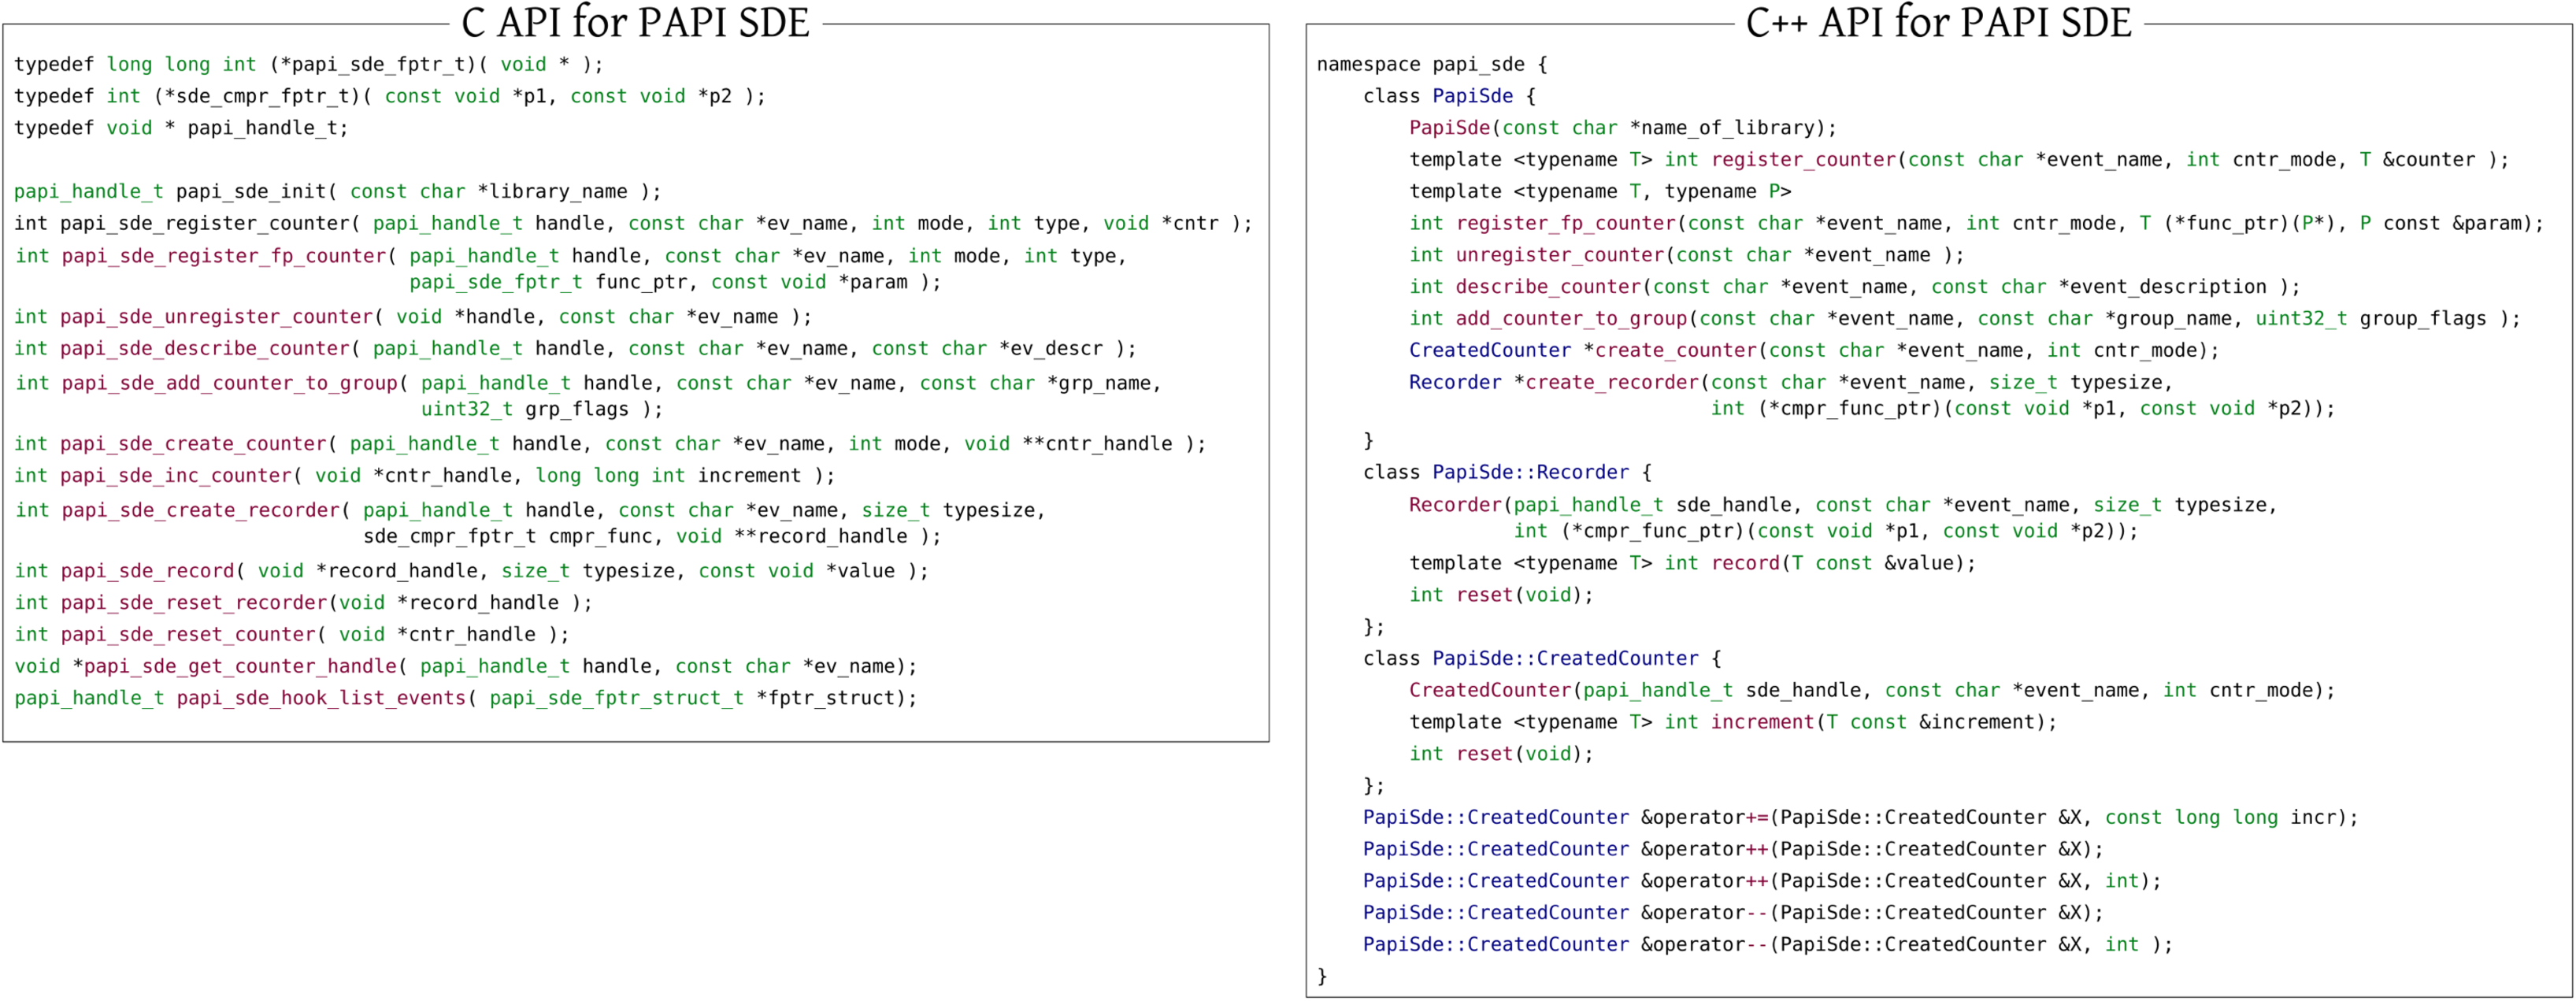
\includegraphics[width=0.88\linewidth]{projects/2.3.2-Tools/2.3.2.06-EXA-PAPI/papi_sde.pdf}
\caption{Existing PAPI SDE C API and new SDE C++ API.}
\label{fig:papi_sde}
\end{center}
\end{figure}


\paragraph{Recent Progress}

The Exa-PAPI team is in the process to prepare a major release---PAPI 7.0.0---scheduled
to be shipped in November 2021. For this release, the team has  
designed and developed a C++ API for utilizing PAPI's software-defined events (SDEs) 
from within third-party libraries and applications that are written in C++. 
This is a major addition to the already implemented and released 
C and FORTRAN APIs for the PAPI SDE functionality (shipped with PAPI 6.0.0 in 
March 2020). The example code in Figure~\ref{fig:papi_sde} demonstrate  the 
C and C++ API for PAPI SDEs. 
%

\vspace{10pt}
Furthermore, PAPI 7.0.0 will release newly developed support for the latest monitoring
features on the Intel Gen9 GPUs. 
This was accomplished under NDA and in very close collaboration with the Intel team. 
The new PAPI capabilities for monitoring Intel Gen9 include GPU hardware 
events, and memory performance metrics (bytes read/written/transferred from/to L3).
Monitoring of GPU and memory performance counters aids developers in producing
more efficient code by profiling the utilization of the latest GPU resources and
diagnosing performance bottlenecks.
The objective of this development was to  
%a mechanism to collect Intel
%GPU performance metrics via PAPI�s well known interface and without any additional
%efforts from the users.
%In our approach, through the PAPI component framework, we 
enable transparent access
to the Gen9 performance and memory metrics via Intel's OneAPI Level-Zero Interface.
A unique feature of this development enables users to apply two different collection modes 
via the PAPI interface:\\
The Time-based Collection Mode:
\begin{itemize}
\item Counter values are aggregated and stored in a buffer.
\item Counter values can be read at any given time during the execution, which means
performance counter monitoring is completely autonomous from the kernels
running in the GPUs.
\end{itemize}
%
The Kernel-based Collection Mode:
\begin{itemize}
\item Counter monitoring is per kernel.
\item Performance counter data is not available during kernel execution but only after
the kernel finishes.
\item In this mode, the Level-Zero API uses internal barriers, which implies, if two
kernels overlap, the execution of the second kernel is pushed out until the first
kernel finishes.
\end{itemize}


\vspace{10pt}
Another major change in PAPI 7.0.0 is the refactoring of the PAPI CUDA component and 
new developments to support NVIDIA compute capability 7.0 and greater. This required
the use of the CUDA/CUPTI 11 Profiling and Perfworks APIs. The PAPI CUDA component 
has been redesigned so that it works in equal measure for NVIDIA compute capabilities 
$<$ 7.0 and $\geq$ 7.0. 
 
 
 \vspace{10pt}
Last but not least, the team designed and implemented PAPI support for FUGAKU's A64FX 
Arm architecture. This work includes the development of new Counter Analysis Toolkit (CAT) 
benchmarks and refinements of PAPI's CAT data analysis; specifically, the extension of 
PAPI's CAT with MPI and ``distributed memory''-aware benchmarks and analysis in order to 
stress all cores/node. The CAT analysis of the A64FX raw hardware counters resulted in the 
definition of 36 new PAPI presets for FUGAKU users.
 
 

\paragraph{Next Steps}

Our next efforts will focus on:
\begin{enumerate}
\item \textbf{Modernize atomics and reduce overhead in PAPI:} 
	When PAPI calls are made from within different thread contexts, PAPI uses internal 
	mechanisms for guaranteeing thread safety. 
	Atomic operations have a central role in these mechanisms, since they introduce less 
	overhead than mutexes. 
	However, the support for atomic operations in the current PAPI framework is limited, 
	and many opportunities are missed. Projects such as ``the atomic\_ops library'' offer a 
	much wider support for atomic operations, which the team plans to leverage in PAPI.

%
\item \textbf{Improved multi-threading and OpenMP support in PAPI}: 
	Beyond the atomic operations for guaranteeing correctness, PAPI will modernize 
	support for threads. PAPI was originally designed in a time when threads were exotic, 
	and OpenMP was nonexistent. The Exa-PAPI team will improve the interoperability with 
	thread systems and OpenMP in particular.

%
\item \textbf{Development of PAPI support for new ECP hardware}:
	Development of new PAPI components, as well as new features in current PAPI 
	components due to underlying vendor interface updates. Development of new PAPI 
	presets (predefined events) for newly released hardware.
\end{enumerate}

\newpage

\subsubsection{\stid{2.08} HPCToolkit} 
\paragraph{Overview} 

The HPCToolkit project is working to develop performance measurement
and analysis tools to help ECP application, library, runtime, and tool
developers understand where and why their software does not fully
exploit hardware resources within and across nodes of extreme-scale
parallel systems. Key deliverables of the project are a suite of
software tools that developers need to measure and analyze the
performance of parallel software as it executes on existing ECP
testbeds and new technologies needed to measure and analyze
performance on forthcoming GPU-accelerated exascale systems.

To provide a foundation for performance measurement and analysis, the
project team is working with community stakeholders, including
standards committees, vendors, and open source developers to improve
hardware and software support for measurement and attribution of
application performance on extreme-scale parallel systems. The
project team has been engaging vendors to improve hardware support
for performance measurement in next-generation GPUs and working
with other software teams to design and integrate new capabilities
into operating systems, runtime systems, communication libraries, and
application frameworks that will enhance the ability of software
tools to accurately measure and attribute code performance on
extreme-scale parallel systems.  Using emerging hardware and software
interfaces for monitoring code performance on both CPUs and GPUs, the project team is
working to extend capabilities to measure and analyze computation, data movement,
communication, and I/O as a program executes to pinpoint scalability
bottlenecks, quantify resource consumption, and assess
inefficiencies.

\paragraph{Key  Challenges}

Today's fastest supercomputers and forthcoming exascale systems all
employ GPU-accelerated compute nodes. Almost all of the 
computational power of GPU-accelerated compute nodes comes from GPUs rather than CPUs.
GPU-accelerated compute nodes have complex memory hierarchies that include 
multiple memory technologies with different bandwidth and latency characteristics. In addition, 
GPU-accelerated compute nodes have non-uniform connections between memories and computational elements (CPUs and GPUs). 
Furthermore, three emerging DOE supercomputers (Perlmutter, Aurora, and Frontier) will feature GPUs from different vendors (NVIDIA, Intel, and AMD). 
There are significant differences in the underlying organization of these GPUs as well as their hardware and software support for performance measurement. For
performance tools, the need to support multiple CPU and GPU architectures significantly increases tool complexity.  At the same time, the
complexity of applications is increasing dramatically as developers
struggle to expose billion-way parallelism, map computation onto
heterogeneous computing elements, and cope with the growing complexity
of memory hierarchies. While application developers can employ
abstractions to hide some of the complexity of emerging parallel
systems, performance tools must be intimately familiar with each of
the features added to these systems to improve performance or
efficiency, develop measurement and analysis techniques that assess
how well these features are being exploited, and then relate these
measurements back to software to create actionable feedback that will
guide developers to improve the performance, efficiency, and
scalability of their applications.

\paragraph{Solution Strategy}

Development of HPCToolkit as part of ECP is focused on preparing it
for production use at exascale by enhancing it in several ways. First,
the team is adding new capabilities to measure and analyze
interactions between software and key hardware subsystems in
extreme-scale platforms, including GPUs and the complex memory hierarchies on GPU-accelerated compute nodes. A major focus of this effort is developing new capabilities for 
measurement and analysis of performance on GPUs.
Second, the team is working to improve performance
attribution given optimized code for a large collection of complex node-level programming
models used by ECP developers, including 
vendor specific programming models such as CUDA, HIP, and Data Parallel C++,
open source community programming models such as OpenMP,
and template-based programming models developed at national laboratories such as LLNL's RAJA and Sandia's Kokkos. To support
this effort, the project team is enhancing the Dyninst binary analysis
toolkit, which is also used by other ECP tools. A major focus of this effort 
is to support analysis of GPU binaries. Third, the team is
improving the scalability of HPCToolkit so that it can be used to
measure and analyze extreme-scale executions. Fourth, the project team
is working to improve the robustness of the tools across the range of
architectures used as ECP platforms. Finally, the project team will
work other ECP teams to ensure that they benefit from HPCToolkit's
capabilities to measure, analyze, attribute, and diagnose performance
issues on ECP testbeds and forthcoming exascale systems.

%\newpage
\paragraph{Recent Progress}

\begin{itemize}

\item
The project team developed a unified GPU monitoring substrate. Upon this substrate, they developed support for collecting summary metrics for 
kernel launches, memory copies, and synchronizations on AMD, Intel, and NVIDIA GPUs.


\item
The project team enhanced support for fine-grained measurement of GPU computations using PC sampling on NVIDIA GPUs and binary instrumentation on Intel GPUs. 
HPCToolkit uses instruction-level measurements to reconstruct calling context trees and
parses NVIDIA's extended line map to reconstruct GPU inlining call chains to help developers understand performance of complex GPU kernels.
Figure~\ref{fig:hpctoolkit}(a) shows a calling context for PeleC, an ECP application for adaptive-mesh compressible hydrodynamics code for reacting flows; the highlighted region shows a reconstruction of GPU calling contexts with multiple inlined GPU device functions.

\item
The project team enhanced HPCToolkit for collecting and visualizing traces of both CPU and GPU activity.
Figure~\ref{fig:hpctoolkit}(b) shows a trace of a GPU-accelerated execution of LAMMPS, an ECP application for parallel molecular dynamics simulation, using 512 NVIDIA A100 GPUs. Each GPU kernel is related to the CPU calling context in which it was launched, which helps developers understand the performance of complex applications.

\item
The project team developed a novel approach that utilizes both shared and distributed memory parallelism to analyze and aggregate sparse data representations of performance measurements from every rank, thread and GPU stream in a program execution. 

\item 
The project team improved the reliability of HPCToolkit's hpcrun for monitoring complex dynamic library loading and unloading and interacting with the application when other software tools are present.

\end{itemize}

\begin{figure}[t]
\captionsetup{width=.96\textwidth}
\begin{minipage}[t]{.40\textwidth}
\centering
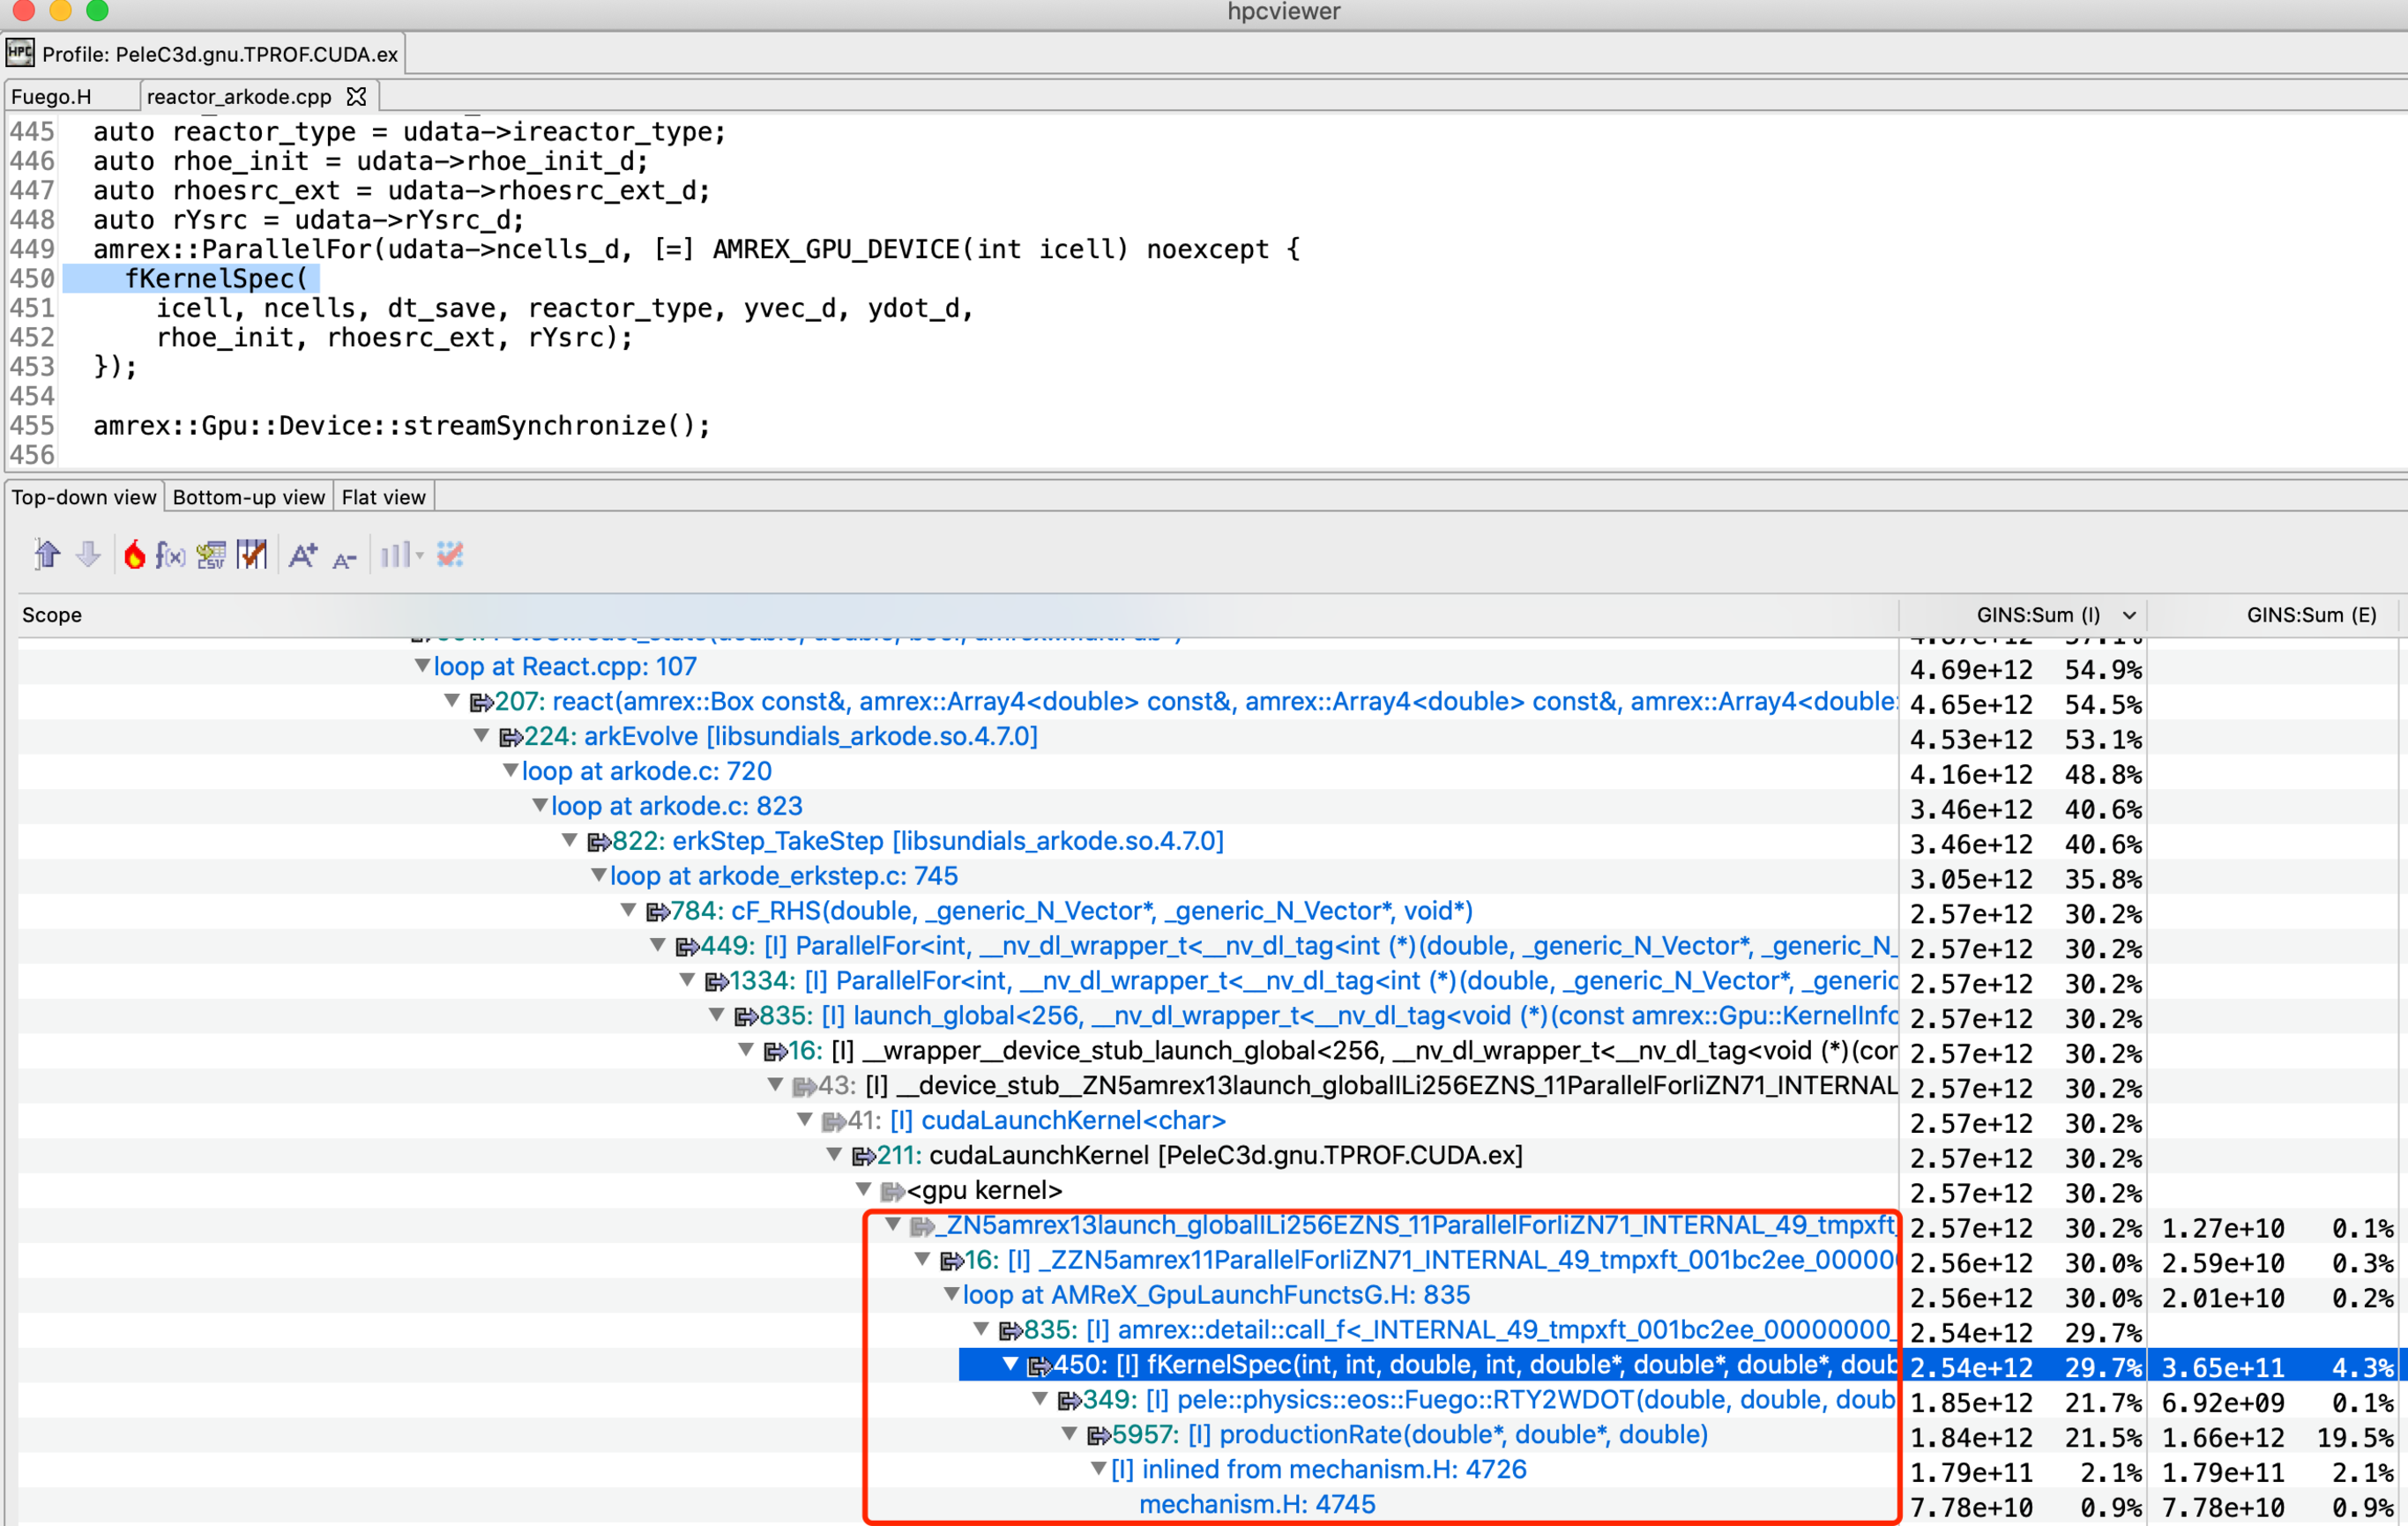
\includegraphics[width=\textwidth]{projects/2.3.2-Tools/2.3.2.08-HPCToolkit/hpctoolkit-pelec-profiles}
\\(a)
\end{minipage}
\hfill
\begin{minipage}[t]{.46\textwidth}
\centering
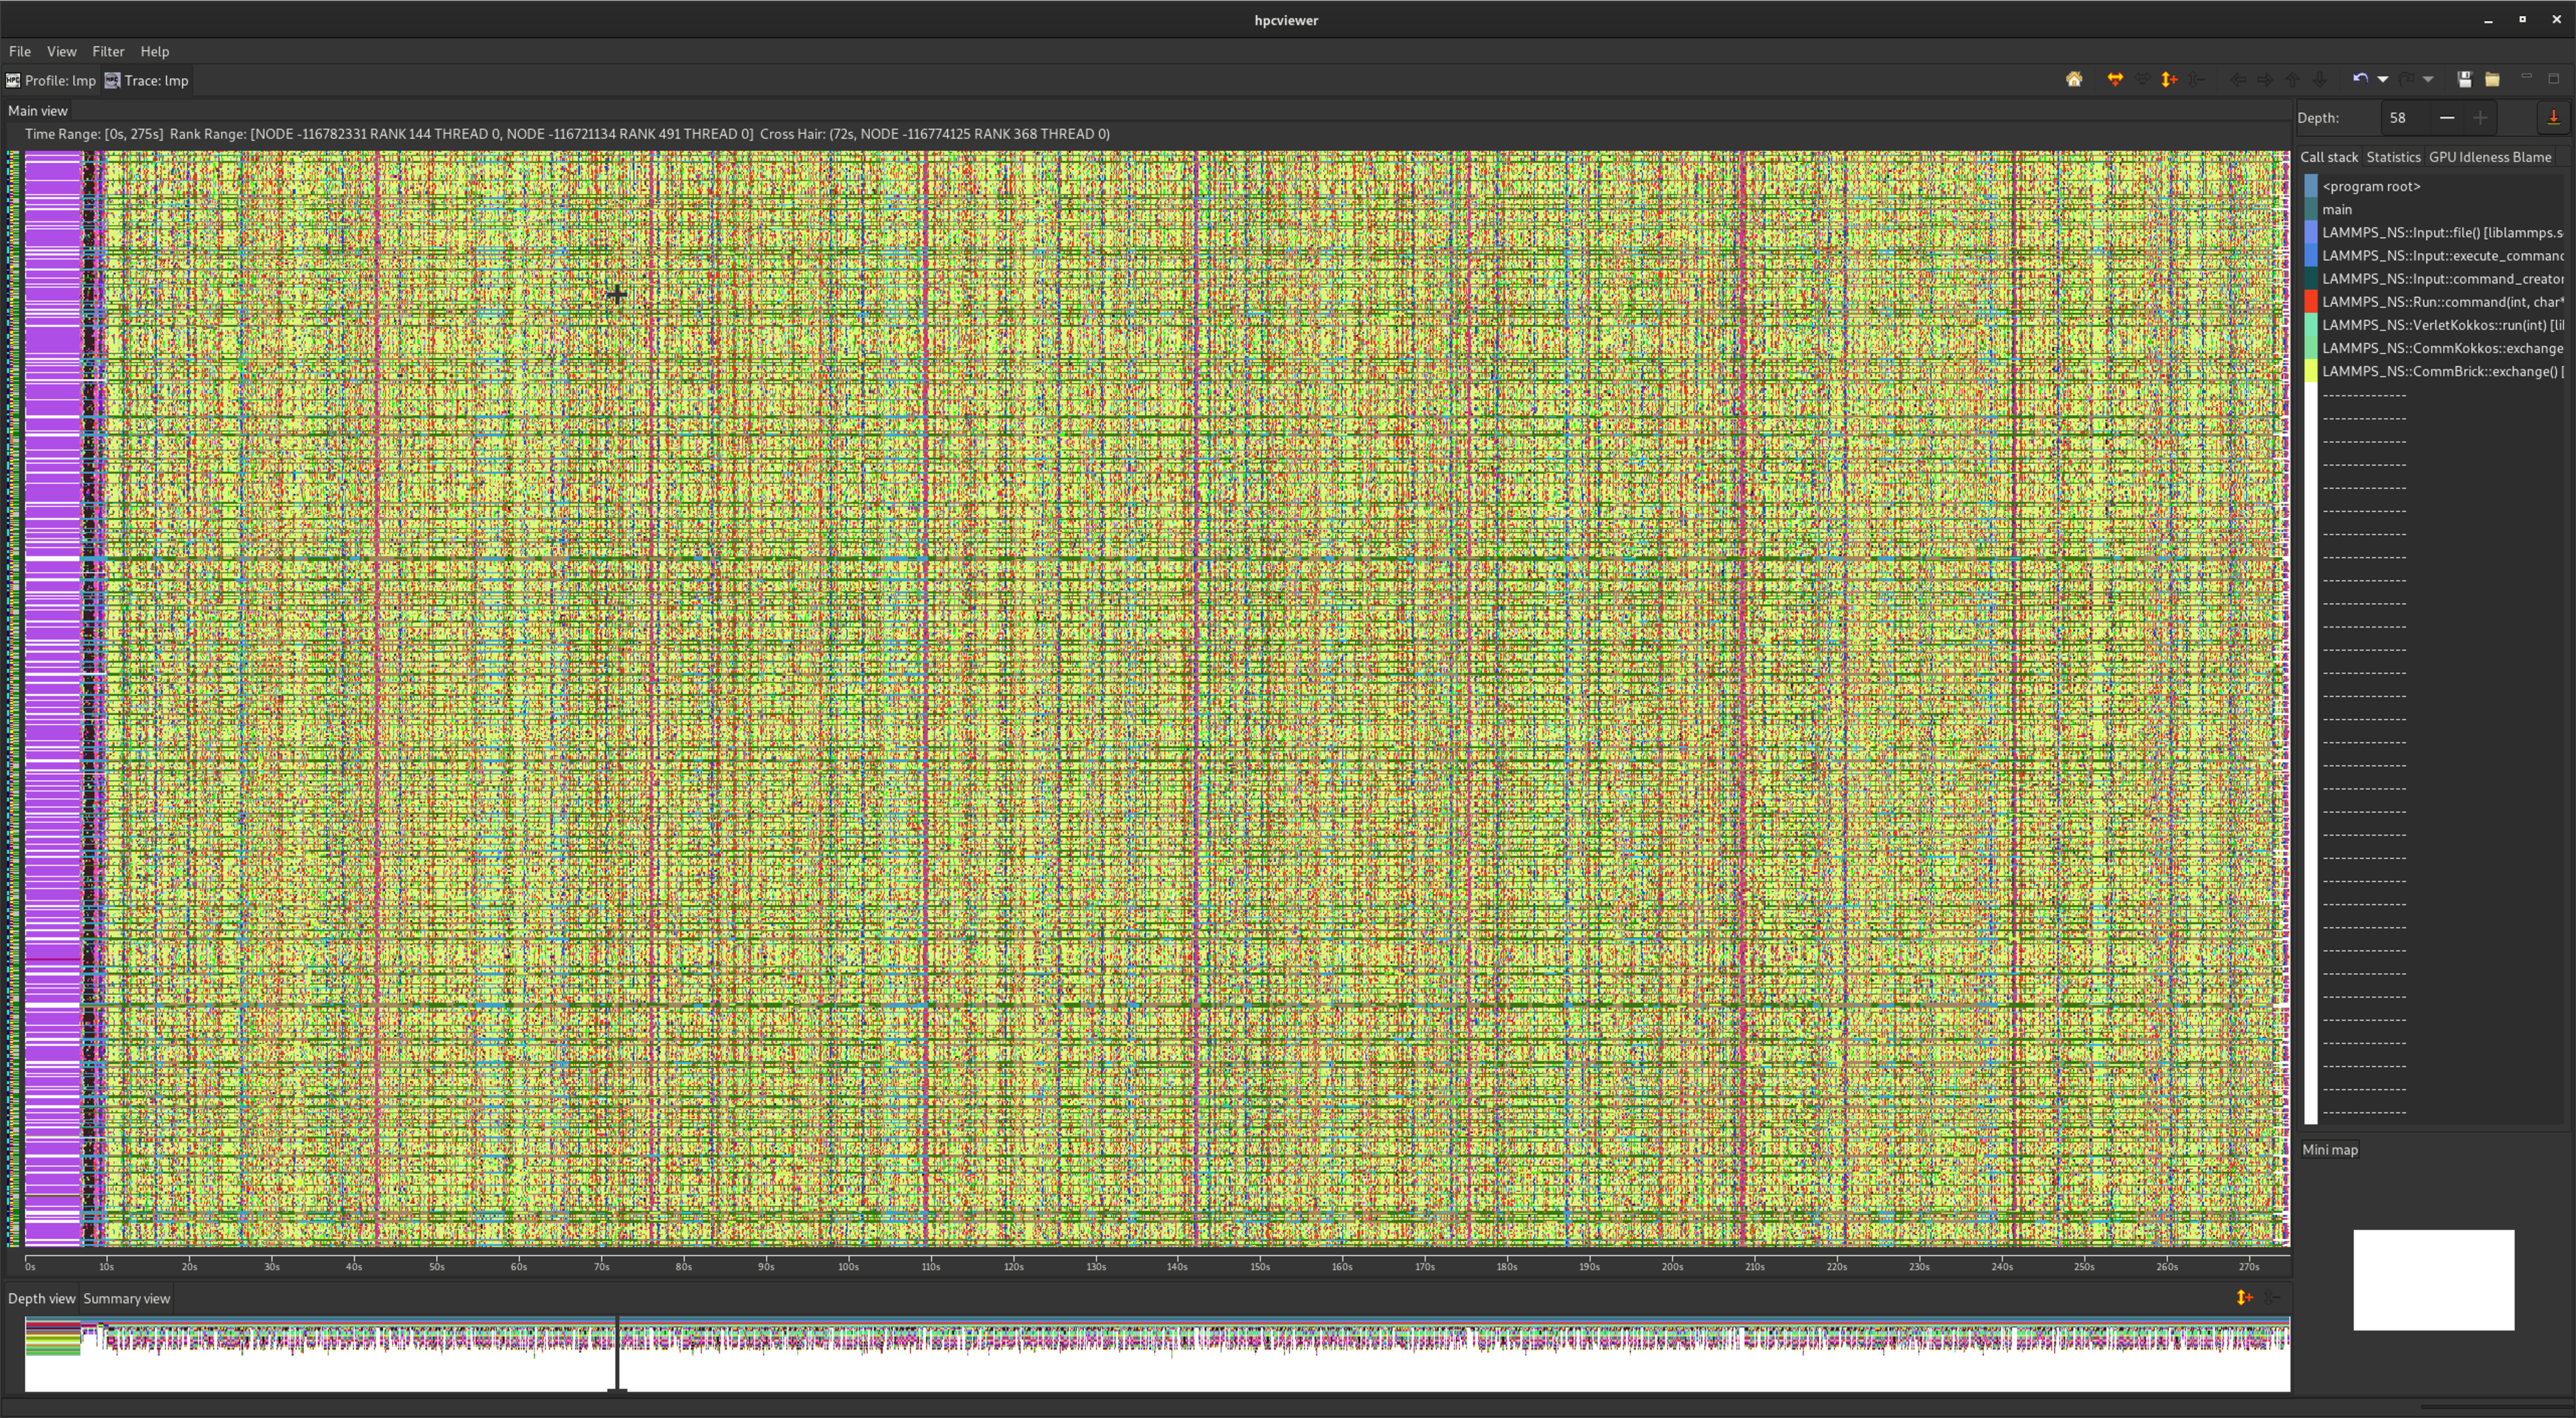
\includegraphics[width=\textwidth]{projects/2.3.2-Tools/2.3.2.08-HPCToolkit/hpctoolkit-lammps-traces}
\\(b)
\end{minipage}
\caption{(a) 
HPCToolkit's \texttt{hpcviewer} showing a detailed attribution of GPU performance metrics in a 
profile of PeleC.
(b) HPCToolkit's \texttt{hpctraceviewer} showing CPU and GPU trace lines for LAMMPS.}
\label{fig:hpctoolkit}
\end{figure}

\paragraph{Preliminary Experiences on Early Access systems}

\subparagraph{HPCToolkit}
The project team is working to deliver tracing and profiling of GPU activity atop AMD's \texttt{rocTracer} API and to assess GPU kernel activity using hardware counters using AMD's \texttt{rocProfiler} API. 
HPCToolkit builds and runs on the Spock and Crusher early access systems. 
At present, the project team is working closely with AMD to 
resolve issues measuring GPU-accelerated
applications with the \texttt{rocTracer} and \texttt{rocProfiler} APIs
by providing test cases that highlight issues of concern.

In addition, the project team has been collaborating with AMD to develop
support for monitoring the performance of OpenMP offload in the
runtime for AMD's AOMP compiler. The code is integrated into AMD's development
branch and has been submitted upstream
for integration into LLVM OpenMP.  A development branch of HPCToolkit
uses this support to attribute GPU activity to OpenMP \texttt{target}
regions. The HPCToolkit project team is working to integrate this 
emerging capability into a forthcoming release.
\subparagraph{Dyninst}
Dyninst builds and runs on the Spock and Crusher early access systems. 
HPCToolkit uses Dyninst to analyze AMD CPU binaries to attribute 
performance measurements to source code contexts, 
including functions, loops, and lines.   


\paragraph{Next Steps}
Next steps for each effort have already been identified.
%
The team will integrate GPU measurement and analysis capabilities using hardware counters.
%
Solutions for fine-grained computation measurement on Intel GPUs will be improved, and the team will explore new solutions for fine-grained measurement on AMD GPUs.
%
Efforts will continue to refine the reliability and performance of monitoring operations on dynamic libraries.
%
The team will work with the open-source community to upstream the team's GPU measurement support into the community version of the \texttt{libomptarget} offloading library.
%
Finally, we will continue to work with DOE and platform vendors to evaluate and refine software interfaces for measuring GPU performance.



\newpage
\subsubsection{\stid{2.10} PROTEAS-TUNE: Programming Toolchain for Emerging Architectures and Systems} 

\paragraph{Key  Challenges:}
Programmer productivity and performance portability are two of the most important challenges facing users of future exascale computing platforms. Application developers targeting ECP architectures will find it increasingly difficult to meet these two challenges without integrated capabilities that allow for flexibility, composability, and interoperability across a mixture of programming, runtime, and architectural components. 

\paragraph{Solution Strategy:}
The PROTEAS-TUNE project was formed as a strategic response to this challenge. (The PROTEAS-TUNE project is the result of merger in FY20 of two previous ECP projects: PROTEAS [PROgramming Toolchain for Emerging Architectures and Systems] and Y-Tune: Autotuning for Cross-Architecture Optimization and Code Generation.) 
This project has three high-level goals. First, PROTEAS-TUNE will provide a programming pathway to anticipated exascale architectures by addressing programmability and portability concerns of emerging technology trends seen in emerging architectures. In particular, the project focuses on improvements to LLVM and OpenACC. Additionally, the team has significant experience with CUDA, OpenCL, and other programming models that will enable ECP applications teams to explore programming options to find the most effective and productive approaches without constraining programming models or software solutions. Second, PROTEAS-TUNE will prototype an integrated programming framework strategy will deliver solutions on these emerging architectures that will be further refined for these architectural capabilities, and make sure that they transition to vendors, standards activities, applications, and facilities. Thirdly, PROTEAS-TUNE includes autotuning which makes it possible to separate a high-level C/C++/FORTRAN implementation from architecture-specific implementation (OpenMP, OpenACC, CUDA, etc.), optimization, and tuning. It also provides a flexible programming framework and integrated toolchain that will provide ECP applications the opportunity to work with programming abstractions and to evaluate solutions that address the exascale programming challenges they face. 


Specifically, the PROTEAS-TUNE focuses on seven thrusts to improve capabilities and performance portability for applications on exascale architectures: 

\begin{itemize}
\item 
    Improve the core-LLVM compiler ecosystem; 
\item 
	Design and implement the OpenACC heterogeneous programming model for C/C++ in Clang/LLVM (Clacc);
\item 
    Design and implement the OpenACC heterogeneous programming model for Fortran in Flang/LLVM (Flacc);  
    
\item 
	Use performance modeling and optimization to enable code transformation and performance portability;
\item 
	Refine autotuning for OpenMP and OpenACC programming models in order to directly target challenges with heterogeneous architectures;
\item 
    Improve performance measurement and analysis tools (TAU) for the target exascale architectures and apply it to applications to improve performance;
\item 
    Develop and implement portable software abstractions (Papyrus) for managing persistent memory;
\item 
    Aggressively engage applications, SDK, vendor, and software teams to demonstrate and deploy; and,
\item
    in collaboration with SOLLVE and Flang, develop a DOE ECP fork of LLVM that will be the clearinghouse for ECP modifications of LLVM  (see \url{https://github.com/llvm-doe-org}).
    
\end{itemize}

Importantly, the team’s solutions are based on significant, continuing work with LLVM, OpenACC, OpenMP, ARES HLIR, OpenARC, TAU, SuRF and CHiLL. The team has extensive experience and a demonstrated track record of accomplishment in all aspects of this proposed work including existing software deployments, interaction with application teams, vendor interaction, and participation in open source community and standards organizations. Also, the team champions its successful solutions in ECP procurements, community standards, and open-source software stacks, like LLVM, in order to improve their use.

%\paragraph{Key  Challenges:}
%Programmer productivity and performance portability are two of the most important challenges facing applications targeting future Exascale computing platforms. Application developers targeting evolving ECP architectures will find it increasingly difficult to meet these dual challenges without help from integrated capabilities that allow for flexibility, composability, and interoperability across a mixture of programming, runtime, and architectural components. In particular, an integrated programming toolchain is critical for Exascale delivery. First, it will provide a programming pathway to anticipated Exascale architectures by addressing programmability and portability concerns of emerging technology trends seen in pre-procurement machines. It will also enable ECP applications teams to explore programming options to find the most effective and productive approaches without constraining programming models or software solutions. Second, an integrated programming framework strategy will deliver solutions that will be further refined for the architecture capabilities known to be in the system procurement. This is essential for maintaining developer productivity and attaining performance portability as ECP requirements evolve.
%
%
%\paragraph{Solution Strategy:}
%The PROTEAS (\textit{PROgramming Toolchain for Emerging Architectures and Systems}) project is a strategic response to the continuous changes in architectures and hardware that are defining the landscape for emerging ECP systems. PROTEAS is a flexible programming framework and integrated toolchain that will provide ECP applications the opportunity to work with programming abstractions and to evaluate solutions that address the Exascale programming challenges they face. Specifically, the PROTEAS objectives are to
%
%\begin{enumerate}
%    
%    \item Provide productive and performance-portable programming solutions based on directive-based methodologies that support current language paradigms and flexible prototyping of interfaces specifically directed at heterogeneous and manycore processors, deep memory hierarchies, and nonvolatile memory systems (NVM);
%    
%    \item Provide integrated performance assessment solutions for these programming systems that will enable automatic performance analysis and performance-driven optimization;
%    
%    \item Provide an integrated programming toolchain that is powerful enough to prototype the above solutions, while flexible enough to extend its functionality over time;
%    
%    \item Refine our toolchain and solutions through engagement with ECP applications teams who will evaluate prototypes, provide feedback, promote application readiness, and facilitate use of ECP prototype and eventual production machines; and,
%    
%    \item Champion our successful solutions in ECP procurements, community standards (e.g., OpenACC, OpenMP), and open-source software stacks (e.g., LLVM).
%    
%\end{enumerate}
%
%Our team has started with a strong existing base of relevant technological and software capabilities. Importantly, our solutions are based on our significant, continuing work with LLVM, ARES HLIR, OpenARC, and TAU. We have extensive experience and a demonstrated track record of accomplishment in all aspects of this proposed work including existing software deployments, interaction with application teams, vendor interaction, and participation in open source community and standards organizations.
%
%Our strong emphasis on delivering an effective toolchain to application developers within the next few years emphasizes the importance of adopting an integrated programming solution that will be further refined for the architecture capabilities known to be in the Exascale system procurement. We will develop an integrated system (i.e. compilers, runtime systems, debuggers, and performance tools) suitable for deployment in the 2021 timeframe. The experience gained from this development will inform vendor collaborations, proposals to standards committees, and existing open source software to make key elements of our developed technology ready for ECP deployment, either from vendors, through the ECP SDKs, or directly from other open-source venues.
%
%While PROTEAS will be oriented towards foreseeable architectural trends, it will not lock in to specific choices that will constrain what new hardware features it can address. Rather, it is important for the programming framework to embody interoperability, open interfaces, and flexibility in the toolchain, allowing it to pursue high-value solutions as opportunities arise and thereby achieve Exascale performance potential. 

\paragraph{Recent Progress:}

Our recent work has focused on six topics:

\begin{enumerate}
    
    \item OpenACC and Clacc~\cite{clacc:2018:denny}. Develop production-quality, standard-conforming OpenACC compiler and runtime support as an extension of Clang/LLVM. See \S\ref{s:clacc}.
    
    \item OpenACC and Flacc. Develop production-quality, standard-conforming OpenACC compiler and runtime support as an extension of Flang/LLVM. 

    \item Performance analysis with Tau by adding additional functionality for new architectures. 
    Improve a widely-used performance analysis framework by adding functionality for new architectures and software systems.
    See \S\ref{subsubsect:tau}.

    \item Improving LLVM. In collaboration with numerous other ECP projects, PROTEAS is contributing improvements to the LLVM compiler infrastructure. These improvements include simple bugfixes to the existing infrastructure, monitoring Flang progress, developing Clacc (see \S\ref{s:clacc}), developing Flacc (See \S\ref{s:flacc}), and developing a DOE ECP fork of LLVM for our work.
    
    \item Papyrus~\cite{Kim:2017:DIP,Kim:2017:PHP} for portability across NVM architectures. 
Develop a portable interface to NVM architectures to provide massive, persistent data structures as required by many applications.
See \S\ref{s:papyrus}.

    \item Outreach and collaboration with ECP applications teams. 
    We have interacted with over a dozen applications teams to help prepare their applications for ECP. See \S\ref{s:clacc}, \S\ref{s:papyrus}, and \S\ref{subsubsect:tau}.
    
\end{enumerate}

\paragraph{Next Steps:}

Our next efforts are:

\begin{enumerate}
	\item Clacc. Continue developing OpenACC support by lowering OpenACC directives to use the existing LLVM OpenMP infrastructure.
    
    \item Flacc. Continue developing OpenACC support by finishing the development of the  OpenACC dialect for MLIR and beginning to develop the runtime system on the existing LLVM OpenMP infrastructure.
    
	\item Papyrus. Improve support for versioning and other performance improvements.
    
    \item Tau. Improve performance instrumentation for deep memory hierarchies in Tau, focusing primarily on various GPUs and emerging NVM.
    
    \item ECP LLVM fork. Finish consolidation of ECP activities into the ECP LLVM fork, and start basic support for continuous integration.

\end{enumerate}

\subsubsection{\stid{2.10} PROTEAS-TUNE: LLVM} 

\paragraph{Overview}

LLVM, winner of the 2012 ACM Software System Award, has become an integral part of the software-development ecosystem for optimizing compilers, dynamic-language execution engines, source-code analysis and transformation tools, debuggers and linkers, and a whole host of programming-language and toolchain-related components. Now heavily used in both academia and industry, where it allows for rapid development of production-quality tools, LLVM is increasingly used in work targeted at high-performance computing. LLVM components are integral parts of the programming environments on our upcoming Exascale systems, and smaller-scale systems as well, being not only popular open-source dependencies, but are critical parts of the commercial toolchains provided by essentially all relevant vendors.

\paragraph{Key Challenges}

LLVM is well suited to the compilation of code from C++ and other languages on CPU hardware, and for some models, GPU hardware, but lacks the kind of high-level optimizations necessary to enable performance-portable programming across future architectures.
\begin{itemize}
\item LLVM lacks the ability to understand and optimize parallelism constructs within parallel programs.
\item LLVM lacks the ability to perform high-level loop transformations to take advantage of complex memory hierarchies and parallel-execution capabilities.
\end{itemize}

Without these abilities, code compiled well for LLVM must be presented to the compiler in a form already tuned for a specific architecture, including expressions of parallelism suited for the particular characteristics of the target machine. It is, however, unfeasible to tune our entire workload of applications in this way for multiple target architectures. Autotuning helps this problem by allowing dynamic analysis to supplement static cost modeling, which is always fundamentally limited, but without the ability to perform complex transformations, both the parallel and serial execution speed of the resulting programs will be suboptimal.

There are two remaining challenges that we are addressing: The first is that deploying autotuning relying on source-to-source transformations is difficult because maintaining these separate source kernel versions is practically difficult. The second is that, as a general matter, performance improvements can be obtained by specializing code and runtime as opposed to limiting ourselves to ahead-of-time code generation.

\paragraph{Solution Strategy}
We are developing two significant enhancements to LLVM's core infrastructure, and many other LLVM components. These enhancements are grouped into two categories:
\begin{itemize}
\item Enhancements to LLVM's inter-procedural analysis, and an improved representation of parallelism constructs, to allow LLVM to propagate information across boundaries otherwise imposed by parallelism constructs, and to allow LLVM to transform the parallelism constructs themselves.
\item Enhancements to LLVM's loop-optimization infrastructure to allow the direction of a sequence of loop transformations to loop nests, exposing these features to users through Clang pragmas (in addition to being available at an API level to tools such as autotuners), enabling those transformations to execute as specified, and otherwise enhancing the loop-optimization infrastructure.
\end{itemize}

As part of this project, we're investigating both fundamental intermediate
representation (IR) level enhancements (as part of the Kitsune development), as
well as runtime call aware optimizations that deal with the classical lowering
of parallelism into runtime calls. The latter mechanism is being implemented
upstream as an OpenMP optimization pass, while the Kitsune work is, at present,
more exploratory.

To address autotuning and the need for code specialization, we are developing a just-in-time compilation technology with integrates naturally with the C++ language as well as embedding of (domain specific) languages into C/C++ programs.

\paragraph{Recent Progress}

For parallelism, we have implemented several new features in upstream LLVM
including an OpenMP-aware optimization pass that performs various optimizations
specific to OpenMP code on the host and device (=GPU)~\cite{OpenMPOpt2020}. It
is run by default with medium and high optimizations enabled (``-O2'' and
``-O3''). In addition to transformations it will provide user feedback in form
of optimization remarks (``-Rpass=openmp-opt'')

Extension to the Attributor inter-procedural optimization framework that
transparently applies transformations across the  boundary between sequential
and parallel code. This upstream work will reduce the overhead parallelism
introduces due to missed classical optimizations~\cite{giorgis2020}.

We prototyped heterogeneous LLVM-IR modules which allow host and device code to
coexist in the same LLVM-IR file and therefore be optimized with a holistic
view. Our approach was already discussed with the community and needs to be
further refined and tested.

For loop optimizations, we have implemented several new features in LLVM and
Clang, including the OpenMP 5.1 ``tile'' directive and clang pragma syntax for
exploration of future transformations not yet available through the OpenMP
standard. Most of these enhancements are in papers
(~\cite{kruse2018user,kruse2018loop} and in several forums directly to the LLVM
community.

In a more forward looking approach we prototyped a loop-hierarchical IR for
LLVM which we also present and discuss in various LLVM community forums.

To facilitate autotuning (ref. Section \ref{sec:PROTEAS_TUNE_AUTOTUNING}), we
implemented a loop nest information extraction tool for
LLVM-IR~\cite{kruse2020search}.

We have developed a prototype C++ compiler, based on Clang, supporting an
extension that enables programmers to embed (domain specific) languages inside
their ``C-like'' programs~\cite{finkel2020dsl}. That is, we allow a new type of
Clang plugin to bridge the gap between classical code, e.g., C or C++, and code
written in a different language, e.g., a quantum or tensor domain specific
language (DSL). The latter two examples have been successfully prototyped as
well.

All our efforts have also been featured in many talks, tutorials, and so on at
LLVM developers' meetings over the last couple of years.

\paragraph{Next Steps}
We will continue to prototype implementations, discuss them with the LLVM
community, and then refine them for integration in upstream LLVM.

For the C++ JIT technology, we will also continue to pursue standardization at
the C++ standards committee.

In addition, we are implementing autotuning technology based on the loop
transformation improvements, and other improvements developed by this project.
This will enable an easy-to-use autotuning capability for applications on
Exascale systems.

Parallelism specific optimizations will further be improved through Attributor
enhancements upstream and more capabilities for the OpenMP-aware aware
optimization pass. Generalization of the latter to other parallel models is
planned as well.

To enable optimizations across the host-device boundary we are continuing to
work on heterogeneous LLVM-IR modules in order to integrate them into upstream
LLVM.


%\end{document}

\subsubsection{\stid{2.10} PROTEAS-TUNE - Clacc: OpenACC in Clang and LLVM}\label{s:clacc}

%\newcommand{\todo}[1]{\textbf{\textcolor{red}{#1}}} use todonotes package

\paragraph{Overview}

Heterogeneous and manycore processors (e.g., multicore CPUs, GPUs,
Xeon Phi, etc.) are becoming the de facto architectures for current
HPC platforms and future Exascale platforms.  These architectures are
drastically diverse in functionality, performance, programmability,
and scalability, significantly increasing the complexity that ECP app
developers face as they attempt to fully utilize available hardware.

A key enabling technology pursued as part of PROTEAS-TUNE is OpenACC.
While OpenMP has historically focused on shared-memory multi-core,
OpenACC was launched in 2010 as a portable programming model for
heterogeneous accelerators.  Championed by institutions like NVIDIA,
PGI, and ORNL, OpenACC has evolved into one of the most portable and
well recognized programming models for accelerators today.

Despite the importance of OpenACC, the only non-academic open-source
OpenACC compiler cited by the OpenACC website is
GCC \cite{openaccOrgTools}.  However, GCC has lagged behind commercial
compilers, such as NVIDIA's, in providing production-quality support
for the latest OpenACC specifications
\cite{openACCValidationSuite}.  Moreover, GCC is known within the compiler
community to be challenging to extend and, especially within the DOE,
is losing favor to Clang and LLVM for new compiler research and
development efforts.

\textit{Clacc}~\cite{clacc:2018:denny} is a major component of
PROTEAS-TUNE.  Overall, the goal is to build on Clang and LLVM to
develop an open-source, production-quality OpenACC compiler ecosystem
that is easily extensible and that utilizes the latest research in
compiler technology.  Such an ecosystem is critical to the successful
acceleration of ECP applications using modern HPC hardware.  The
PROTEAS-TUNE objectives for Clacc are:

\begin{enumerate}

\item Develop production-quality, standard-conforming OpenACC
compiler, runtime, and profiling support as an extension of Clang and
LLVM.  Two compilation modes are being developed: (a) traditional
mode, which produces a binary, and (b) source-to-source mode, which
produces OpenMP source.

\item As part of the design, leverage the Clang ecosystem to enable
the future construction of source-level OpenACC tools, such as pretty
printers, analyzers, lint tools, debugger extensions, and editor
extensions.

\item Throughout development, actively contribute improvements to the
OpenACC specification, and actively contribute mutually beneficial
improvements to the upstream Clang and LLVM infrastructure.

\item As the work matures, contribute OpenACC support itself to
upstream Clang and LLVM so that it can be used by the broader HPC and
parallel programming communities.

\end{enumerate}

\paragraph{Key Challenges}

\begin{enumerate}

\item \textbf{OpenACC Support:} Developing production-quality,
standards-conforming OpenACC compiler and runtime support is a large
undertaking.  Complicating that undertaking further is the need for
optimization strategies that are competitive with existing commercial
compilers, such as NVIDIA's, which have been developed over many years
since before the conception of the OpenACC standard.

\item \textbf{Source-to-Source:} Lowering OpenACC to OpenMP
significantly reduces the effort to implement OpenACC and offers
additional capabilities, such OpenACC support for proprietary OpenMP
compilers.  However, not all OpenACC features are actually
representable in OpenMP.  Moreover, there are several challenges from
Clang's AST, the source-level representation.  First, it was designed
to be immutable.  Second, the AST represents the source after
preprocessor expansions, which harm readability and can prevent
compilation with other compilers.  Third, sophisticated analyses and
optimizations are critical for lowering OpenACC's descriptive language
to the more prescriptive language of OpenMP, but these are best
implemented at the level of LLVM IR not the Clang AST.

\item \textbf{Production-Quality:} Clang and LLVM are sophisticated tools
with a complex codebase and a large team of developers who diligently screen
contributions to maintain a clean design and correct operation.  As for any
production-quality compiler, developing and contributing improvements to
Clang and LLVM can be significantly more challenging and time-consuming than
for research-quality compilers.

\item \textbf{OpenMP Alternative:} We believe that OpenACC's current
momentum as the go-to directive-based language for accelerators will
continue into the foreseeable future.  Nevertheless, some potential OpenACC
adopters hesitate over concerns that OpenACC will one day be replaced by
OpenMP features.  A tool to migrate OpenACC applications to OpenMP could
alleviate such concerns, encourage adoption of OpenACC, and thus advance
utilization of acceleration hardware in ECP applications.

\end{enumerate}

\paragraph{Solution Strategy}

~
\vspace{-1em}

\begin{tabular}{@{\hspace{-1.5em}}p{.6\textwidth}p{.4\textwidth}@{}}

\begin{enumerate}

\item A key Clacc design feature is lowering OpenACC to OpenMP.
Benefits include:

\begin{enumerate}

\item By building on Clang and LLVM's OpenMP support, it reduces the
effort necessary to construct a production-quality OpenACC
implementation.

\item It enables OpenACC support on OpenMP compilers other than Clang,
including proprietary compilers.

\item It facilitates repurposing existing OpenMP static analysis and
debugging tools for the sake of OpenACC.

\item It facilitates porting applications from OpenACC to OpenMP to
alleviate the aforementioned concerns about developing applications in
OpenACC.

\end{enumerate}

\end{enumerate}

&

\raisebox{-\totalheight}{\includegraphics[scale=.3]{projects/2.3.2-Tools/2.3.2.10-PROTEAS-YTUNE/clacc.png}}

\end{tabular}

\vspace{-1em}

\begin{enumerate}

\setcounter{enumi}{2}

\item To handle Clang's immutable AST, Clacc's design includes a
TransformACCToOMP component, which reuses Clang's TreeTransform
feature, which was originally designed for C++ template
specialization.

\item To avoid preprocessor expansions in source-to-source mode, Clacc
includes a RewriteOpenACC component, which reuses a Clang feature
called Rewrite.

\item To represent OpenACC features not covered by the OpenMP
standard, Clacc is developing original OpenMP extensions.  To utilize
LLVM IR analyses and optimizations, Clacc first translates OpenACC to
our extended OpenMP, which Clacc then translates to LLVM IR.

\item To stage our development effort, we are initially implementing
Clacc with two simplifications: we are implementing a prescriptive
OpenACC interpretation for correct behavior, and we are implementing
for C.  We will then extend Clacc with necessary analyses for a
descriptive interpretation and for C++.

\item Throughout Clacc development, we are continuously integrating the
latest upstream Clang and LLVM changes, and we are running and
extending the Clang and LLVM test suites to detect regressions and
incompatibilities.  We are also investigating OpenACC
benchmarks \cite{specAccel} and validation test
suites \cite{openACCValidationSuite} to ensure correct OpenACC
behavior and good performance.

\end{enumerate}


\paragraph{Recent Progress}

\begin{enumerate}
\item
  Extended Clacc to support additional OpenACC features, most notably
  the OpenACC runtime library routines, but also various directives,
  clauses, environment variables, and associated profiling interface
  functionality.  Developed various OpenMP extensions to support this
  work.
\item
  Extended Clacc's OpenACC support to AMD GPU offload, and extended
  the LLVM DOE Fork's CI infrastructure to test Clacc on relevant
  platforms, including AMD GPUs and OLCF's Ascent.
\item
  Contributed to Clang and LLVM, including LLVM testing infrastructure
  support and original OpenMP extensions required for OpenACC support.
  Contributed to the OpenACC and OpenMP specifications.
\item
  Collaborated with the OpenACC organization to invite broader
  participation in OpenACC LLVM development.  Efforts include docs for
  the LLVM DOE Fork to guide potential collaborators, co-mentoring a
  Google Summer of Code student, and organizing an OpenACC in LLVM
  mini-workshop.
\end{enumerate}


\paragraph{Next Steps}

\begin{enumerate}
\item
  Continue to implement Clacc support for critical OpenACC features
  based on the needs of ECP and other HPC apps and benchmarks, and
  pursue OpenACC optimizations and C++ support.
\item
  Continue contributions to upstream Clang and LLVM and to the OpenACC
  and OpenMP specifications.
\end{enumerate}

\subsubsection{\stid{2.10} PROTEAS-TUNE - LLVM-DOE: Creating and Maintaining a DOE Fork of LLVM}\label{s:llvm-doe}

\paragraph{Overview}

The ECP funds multiple projects that develop compiler technologies, based on the
popular, open-source LLVM compiler infrastructure project. This ecosystem allows
customization to meet the unique needs of ECP, and a level of well-established
mechanisms to deploy technologies through vendors and at DOE’s leadership
facilities. Importantly, this provides an alternative open-source compiler
ecosystem to those provided by the vendor, thus reducing the dependence on the
vendor’s compilers, timelines, and staff (Risk 10032 that ST product will not
function or meet performance targets).

In addition, most today’s vendors already rely on LLVM as the foundation for
their compiler ecosystems. This means ECP technology has a path back to vendors
via LLVM itself or through a DOE-/ECP-focused fork of LLVM’s open source
repository. This work will focus on deployment to reduce Risk 10020.

More broadly, there are eight LLVM-related projects supported by ECP that have
a risk of not being used if developers cannot easily access their contributions.
This fork of LLVM will provide an opportunity for these projects to work
collectively on establishing synergies, interoperability, address the unique
needs of ECP, and mechanisms for making contributions back into the mainstream
LLVM code base. The tasks to setup the DOE Fork of LLVM are as follows:

\begin{enumerate}

\item Set up a fork of the llvm-project upstream repository (see \url{https://github.com/llvm-doe-org}).

\item Enable continuous integration for the fork on various hardware of       interests.

\item Enable LLVM ECP related projects to be able to push and test branches.

\item Setup status information for the continuous information results.

\end{enumerate}


\paragraph{Solution Strategy}

%\begin{enumerate}

The DOE LLVM repository is set up on GitHub as a fork of the llvm-project
      main repository also hosted on GitHub. This makes it easier to have a
      seamless synchronization with the main repository and keep all the
      GitHub main-fork integrated features.
%
The GitHub repository is automatically mirrored in the GitLab premium
      instance hosted at ORNL.
%
Furthermore, the continuous integration takes advantage of the GitLab CI infrastructure.
      This infrastructure is available on several machines from the ExCL lab as
      well as on Summit and Theta.

%\end{enumerate}


\paragraph{Recent Progress}

%\begin{enumerate}
The fork has been set up with an automatic mirroring with the upstream repository.
The mirroring is using GitHub Actions, and the fork is integrated with E4S releases.
%\end{enumerate}


\paragraph{Next Steps}

%\begin{enumerate}
The team will add continuous integration on more hardware (i.e., most recent versions of Frontier and Aurora test nodes) and
improve the test suite for the CI (e.g., OpenACC tests).
%\end{enumerate}

\subsubsection{\stid{2.10} PROTEAS-TUNE - FLACC and MLIR: Creating and Maintaining OpenACC in LLVM/Flang}\label{s:flacc}

\paragraph{Overview}
Heterogeneous and manycore processors (e.g., multicore CPUs, GPUs,
Xeon Phi, etc.) are becoming the de facto architectures for current
HPC platforms and future Exascale platforms.  These architectures are
drastically diverse in functionality, performance, programmability,
and scalability, significantly increasing the complexity that ECP app
developers face as they attempt to fully utilize available hardware.

A key enabling technology pursued as part of PROTEAS is OpenACC.
While OpenMP has historically focused on shared-memory multi-core,
OpenACC was launched in 2010 as a portable programming model for
heterogeneous accelerators.  Championed by institutions like NVIDIA,
PGI, and ORNL, OpenACC has evolved into one of the most portable and
well recognized programming models for accelerators today.

Despite the importance of OpenACC, the only non-academic open-source OpenACC
compiler cited by the OpenACC website is GCC \cite{openaccOrgTools}.
However, GCC has lagged behind commercial compilers, such as PGI's, in
providing production-quality support for the latest OpenACC specifications
\cite{openACCValidationSuite}.  Moreover, GCC is known within the compiler
community to be challenging to extend and, especially within the DOE, is
losing favor to Clang and LLVM for new compiler research and development
efforts.

Recent efforts to build a Fortran counter-part to Clang in LLVM project have
been accelerated and big chunk of the Flang have been upstreamed.
Directive-based programming model are heavily used in Fortran applications ported
to accelerators. Unlike C and C++, Fortran doesn not have many alternatives.

FLACC proposes to develop a prototype OpenACC 3.0 implementation in Flang based
on MLIR to fill this gap. As the implementation of the OpenMP target offload
feature in Flang does not have a clear path, this work will help in this regard
by sharing code in the MLIR dialects and lowering sections with the Flang and
SOLLVE projects.

\paragraph{Key Challenges}

\begin{enumerate}

\item \textbf{OpenACC Support:} Developing production-quality,
      standards-conforming OpenACC compiler and runtime support is a large
      undertaking. Complicating that undertaking further is the need for
      optimization strategies that are competitive with existing commercial
      compilers, such as PGI's, which have been developed over many years
      since before the conception of the OpenACC standard.

\item \textbf{MLIR:} Flang and the OpenACC support for it rely on the MLIR
      project for the intermediate representation. MLIR has been upstreamed to
      the core LLVM project in early 2020 and it is still actively under
      development. Flang will be the first core frontend relying on MLIR.

\item \textbf{Runtime:} LLVM does not include an OpenACC runtime but only one
      for OpenMP at the moment. This runtime can be generalized to support
      missing OpenACC features. This generalization needs to be accepted by the
      current OpenMP community.

\item \textbf{OpenMP Stability:} As we plan to generalize the OpenMP runtime to
      support OpenACC, we will also rely on various part of the runtime that
      are already here. There has been some concern on the stability of the
      current OpenMP runtime implementation and especially the
      textit{libomptarget} responsible for the target offload part.

\end{enumerate}

\paragraph{Solution Strategy}

~
\vspace{-1em}

\begin{enumerate}

\item Flacc design follows a similar design as the OpenMP implementation for
      Flang. This design includes the following aspects:

\begin{enumerate}
\item An OpenACC MLIR dialect part of the core MLIR project.
\item A lowering from the Flang AST to a mix of FIR and OpenACC MLIR dialect.
\item A progressive lowering from MLIR to LLVM IR with runtime call.
\end{enumerate}

\end{enumerate}

\paragraph{Recent Progress}

\begin{enumerate}
\item OpenACC 3.0 parser is upstreamed to the Flang front-end. It covers the
      full specification and also implements the unparsing feature of Flang.
\item Semantic checking for OpenACC 3.0 is also upstreamed in Flang. While
      implementing this part, a new TableGen backed for directive-based language
      has been contributed upstreamed. This is used by OpenACC and OpenMP for
      both Clang and Flang.
\item Base of the OpenACC MLIR dialect has been introduced upstream. The OpenACC
      dialect is part of the core MLIR project.
\item Discussed Flacc at various ECP, HPC, and LLVM venues.
\end{enumerate}


\paragraph{Next Steps}

\begin{enumerate}
\item Continue the definition of the OpenACC MLIR dialect and complete the
      lowering to it.
\item Start working on the runtime support for OpenACC.
\item Work on the lowering from MLIR to LLVM IR and runtime call.
\end{enumerate}

\subsubsection{\stid{2.10} PROTEAS-TUNE: Autotuning} 
\label{sec:PROTEAS_TUNE_AUTOTUNING}

\paragraph{Overview}

We are developing tools and an application development workflow that separates a high-level C/C++/FORTRAN implementation from an architecture-specific implementation (OpenMP, CUDA, etc.), optimization, and  tuning.   This  approach
will enable Exascale application  developers to express and  maintain a
single, portable implementation of their computation that is also legal code
that can be compiled and run by using standard tools.   The autotuning compiler
and search framework will transform the baseline code into a   collection of
highly-optimized implementations. This reduces the need for extensive manual tuning.
Both code transformation and autotuning are essential in ECP for providing
performance portability on Exascale platforms.  Due to significant architectural
differences in ECP platforms, attaining performance portability may  require
fundamentally different  implementations of software -- different strategies for
parallelization, loop order,  data layout, and exploiting SIMD/SIMT.  A key
concern of ECP is the high cost of developing  and maintaining
performance-portable applications for  diverse Exascale architectures, including
manycore CPUs and GPUs. 
Ideally Exascale application developers would express their
computation separate from   its mapping to hardware, while autotuning compilers can automate this mapping and achieve performance portability.

\paragraph{Key Challenges}
Autotuning has the potential to dramatically improve the performance portability of Petascale and Exascale applications.  To date, autotuning has been used primarily in high-performance applications through tunable libraries or previously tuned application code that is integrated directly into the application.
If autotuning is to be widely used in the HPC community,
support for autotuning must address the software engineering challenges, manage configuration overheads, and continue to demonstrate significant performance gains and portability across architectures.
In particular, tools that configure the application must be integrated into the application build process so that tuning can be reapplied as the application and target architectures evolve.

\paragraph{Solution Strategy}
We are developing pluggable software infrastructure that incorporates
autotuning at different levels: compiler optimization, runtime configuration of application-level parameters and system software.
To guarantee success in the ECP time frame, we are collaborating with
application teams, such as SuperLU and QMCPACK, to impact performance of their
codes and libraries.

The autotuning compiler strategy revolves CHiLL, which has the following distinguishing features:
(1) \textit{Composable transformation and code generation}, such
that the same tool can be applied
to multiple different application domains;
(2) \textit{Extensible to new domain-specific transformations} that can be represented as transformations on loop nest iteration spaces are also
composable with existing transformations;
(3) \textit{Optimization strategies and parameters exposed to autotuning:}
By exposing high-level expression
of the autotuning search space as transformation recipes, the compiler writer, an expert programmer or embedded DSL designer can directly \
express how to compose
 transformations that lead to different implementations.
A part of our efforts in ECP are to migrate these capabilities of CHiLL
into the Clang/LLVM open-source compiler, as well as provide lightweight
interfaces through Python, C++, and REST APIs/web services.

For example, we have developed a \textit{brick data layout library and code generator} for
stencil computations.
Recent trends in computer architecture that favor computation over data movement incentivize high-order methods.  Paradoxically, high-order codes can be challenging for compilers/optimization to attain high performance.  Bricks enable high performance and make fine-grained data reuse and memory access information known at compile time.  The SIMD code generation achieves performance portability
for high-order stencils for both CPUs with wide SIMD units (Intel Knights
Landing) and GPUs (NVIDIA Pascal).  Integration with autotuning attains
performance that is close to Roofline performance bound for both manycore CPU
and GPU architectures and demonstrates strong scaling by reducing on-node data movement in communication.


ytopt/SurF is a machine-learning-based search software package for autotuning that consists of sampling a small number of input parameter configurations, evaluating them, and progressively fitting a surrogate model over the input-output space until exhausting the user-defined time or the maximum number of evaluations. The package is built based on Bayesian Optimization that solves any optimization problem and is especially useful when the objective function is difficult to evaluate. It provides an interface that deals with unconstrained and constrained problems. The software is designed to operate in the master-worker computational paradigm, where one master node fits the surrogate model and generates promising input configurations and worker nodes perform the computationally expensive evaluations and return the outputs to the master node. The asynchronous aspect of the search allows the search to avoid waiting for all the evaluation results before proceeding to the next iteration. As soon as an evaluation is finished, the data is used to retrain the surrogate model, which is then used to bias the search toward the promising configurations.


\paragraph{Recent Progress}


We have pursued the following main activities this year:

\textit{Autotuning capability in LLVM:}
The key idea is to support the use of pragmas in the C++ source to guide transformations to be applied. These can include the types of transformation recipes used in CHiLL, but also parallelization directives for OpenMP and OpenACC that would interact with SOLLVE and PROTEAS. Our initial focus is the implementation of user/tool-directed optimizations in Polly, which is a polyhedral framework in LLVM with some similar features to CHiLL. Several existing open-source LLVM projects allowing for just-in-time (JIT) compilation of C++ code have been identified and are being evaluated for use with autotuning. 

We have successfully used loop transformations directives implemented in Clang (ref. Section \ref{sec:PROTEAS_TUNE_LLVM}) to drive a machine learning process with YtOpt. The correctness of these transformations are checked in the Clang compiler by Polly such that it is not possible to result in wrong results. The search strategies used include a Globally Greedy~\cite{kruse2020search}, random search, beam search and our latest algorithm a customized Monte-Carlo Tree Search~\cite{wu2021autotuning}.
In addition to the PolyBench benchmark suite, we applied the search over a tree-shaped configuration space to three ECP Proxy apps, namely SW4Lite, CoMD and minrAMR with promising results.


\vspace*{.1in}
\noindent
\textit{ytopt/SuRF Supporting Autotuning Search}

Compiler directives such as pragmas can help programmers to separate an algorithm's semantics from its optimization. Pragma directives for code transformations are useful for assisting program optimization and are already widely used in OpenMP. A prototype of user-directed loop transformations using Clang and Polly was implemented for the ECP SOLLVE project.
Polly is LLVM's polyhedral loop optimizer which makes it easy to apply specific transformations as directed by pragmas.
While the SOLLVE team is working on integrating the changes into the official LLVM repository, only few of the changes have been upstreamed yet.
The additional loop transformation directives supported are loop reversal (inverting the iteration order of a loop), loop interchange (permuating the order of nested loops), tiling, unroll(-and-jam), array packing (temporarily copying the data of a loop's working set into a new buffer) and thread parallelization. 
More importantly, it supports composing multiple loop nest transformation in arbitrary order. Vectorization is also supported by LLVM's dedicated loop vectorizer.
These pragmas are intended to make applying common loop optimization technique much easier and allow better separation of a code's semantics and its optimization.

We developed and extended ytopt autotuning framework that leverages Bayesian optimization to explore the parameter space search of LLVM Clang/Polly loop optimization pragmas. We integrated and compared four different supervised learning methods within Bayesian optimization and evaluated their effectiveness. We selected six of the most complex PolyBench benchmarks and apply the newly developed LLVM Clang/Polly loop optimization pragmas to the benchmarks to optimize them. We then used ytopt/SuRF framework to optimize the pragma parameters to improve their performance. The experimental results showed that our autotuning approach outperforms the other compiling methods to provide the smallest execution time for the benchmarks syr2k, 3mm, heat-3d, lu, and covariance with two large datasets in 200 code evaluations for effectively searching the parameter spaces with up to 170,368 different configurations. 

In a number of settings, the search space exposed by the transformation pragmas in LLVM LLVM/Polly’s composable loop optimization is a tree, wherein each node represents a specific combination of loop transformations that can be applied to the code resulting from the parent node's loop transformations. Consequently, Bayesian optimization within ytopt/SuRF will become ineffective. To that end, we have developed ytopt/MCTS, a search algorithm based on Monte Carlo tree search (MCTS). The algorithm consists of two phases: exploring loop transformations at different depths of the tree to identify promising regions in the tree search space and exploiting those regions by performing a local search. Moreover, a restart mechanism is used to avoid the MCTS getting trapped in a local solution. The best and worst solutions are transferred from the previous phases of the restarts to leverage the search history. We compared our approach with breadth-first, beam, global greedy, and random search methods using PolyBench kernels and ECP proxy applications. Experimental results showed that our MCTS algorithm finds pragma combinations with a speedup of 2.3x over Polly's heuristic optimizations on average.

CCS is a autotuning interface that we developed recently for ECP Kokkos library. CCS aims at providing interoperability between autotuning frameworks and applications with autotuning needs. It does so by providing a C interface with which users can describe their tuning problem, but also write their own tuners, possibly in higher-level languages. At the start of the collaboration with Kokkos team, CCS did not match up exactly with the Kokkos model of tuning. In CCS, there were no input types, and the concept of output types, objective space in CCS, was much more complex, providing a system of constraints among those types. It also had a much more complex view of a good run, having an objective space concept to specify how well a given configuration performed. Through codesign, CCS has adopted the input type concept as the features space, while maintaining the full expressiveness of their other concepts. This is progressing to the point where, as uses develop new tuners to the CCS infrastructure, they get the ability to tune Kokkos as well.



\vspace*{.1in}
\noindent
\textit{Brick Library:}
We developed a code generator for the Brick Data Layout library for stencils
that is performance-portable across CPU and GPU architectures, and addresses the
needs of modern multi-stencil and high-order stencil computations. The key
components of our approach that lead to performance portability are (1) a
fine-grained brick data layout designed to exploit the inherent multidimensional
spatial locality common to stencil computations; (2) vector code generation that
can either target wide SIMD CPU instructions sets such as AVX-512 and SIMT
threads on GPUs; and, (3) integration with autotuning framework to apply
architecture-specific tuning. For a range of stencil computations, we show that
it achieves high performance for both the Intel Knights Landing (Xeon Phi) CPU,
and the NVIDIA GPUs \cite{P3HPC_Bricks,zhao2019}. This year we extended the library in multiple ways.
We show that the indirection in the brick data layout permits distinct physical and logical data layouts; we can
therefore store the bricks in memory to reduce the data movement of packing and unpacking during cross-node
communication.  We have demonstrated strong scaling by reducing communication time.  

\paragraph{Next Steps}

We will continue to work with ECP application teams to integrate our tools with their efforts.  In particular,
we are integrating bricks into the Proto system, used in subsurface flows.
Moreover, we are developing online tuning capability for ytopt/SuRF. 

\subsubsection{\stid{2.10} PROTEAS-TUNE - Bricks} 

\paragraph{Overview}
We have developed a source-to-source stencil framework (``texttt{Bricks}'')
  to address the growing gap between memory and computational performance 
  on pre-exascale systems.
The approach uses standard \texttt{C++} code to express stencil loops, 
  then transforms the code to use a different memory alignment and ghost
  zone region to optimize memory and communication performance specifically
  for that stencil kernel~\cite{P3HPC_Bricks,zhao2019,zhaoMPI2019}.
This also provides an opportunity to inject architecture-specific code
  transformations, that can take advantage of SIMD/SIMT, threading,
  virtual memory layouts, and the variety of parameters that are needed to 
  tune for optimal performance.
This is a powerful paradigm for having both a correct legal code base 
  using standard tools and, in combination with the autotuning tools previously described,
  the ability to achieve portable performance on many different 
  platforms with minimal, auto-generated code transformations.

\paragraph{Key Challenges}
\texttt{Bricks} require three primary ingredients for performance portability:
\\
(1) \textit{Stencil kernel metadata} - including stencil radius,
  dimensionality, neighbor dependencies, and other memory access patterns.
  For example, for communication the optimal layout depends on the
  extent of stencil corner coupling and symmetry or reuse.
\\
(2) \textit{Transformation profitability model} - based on the architecture
  characteristics and benchmarks, determining what transformations could
  improve overall throughput, not just maximize flops or bytes moved. 
  This can also be explored using roofline models, auto-tuning, 
  communication-avoiding techniques, etc.
\\
(3) \textit{Back-end optimizations and benchmarks} - knowing what 
  architecture-specific transformations achieve the best roofline performance, 
  and how to isolate and compare those with a known benchmark problem. 
For example, if there
  are special OS or hardware capabilities, like vectorized \textit{shuffle}, 
  or memory \textit{mmap} or \textit{prefetch}, that are required to obtain
  peak performance.

\begin{wrapfigure}{r}{0.35\textwidth}
\begin{center}
  \includegraphics[trim=3mm 5mm 3mm 8mm,width=.33\textwidth]{projects/2.3.2-Tools/2.3.2.10-PROTEAS-YTUNE/Bricks-mpi-parts.pdf}
\end{center}
  \caption{\texttt{Bricks} can be used to map memory onto regions that
  minimize ghost zone packing and MPI message count (2D example).}
\end{wrapfigure}

\paragraph{Solution Strategy}
With \texttt{Bricks}, we have developed a data layout library and code 
  generator for both stencil computations and ghost zone communication.
Recent trends in computer architecture that favor computation over data 
  movement incentivize high-order methods.
Paradoxically, high-order codes can be challenging for compilers/optimization 
  to attain high performance.  
\texttt{Bricks} enable high performance and make fine-grained data reuse and 
  memory access information known at compile time.  
The SIMD code generation achieves performance portability
  for high-order stencils for both CPUs with wide SIMD units (Intel Knights
  Landing and Skylake) and GPUs (NVIDIA Pascal and Volta).  
Integration with autotuning attains performance that is close to Roofline
  performance bound for both manycore CPU and GPU architectures.

\paragraph{Recent Progress}
For optimization of MPI-based communication on exascale proxy systems, 
  we identified several stencil kernels from applications that
  leverage the tuned kernels from previous milestones, and evaluated their
  strong scaling on Theta (Intel KNL) and Summit (NVIDIA V100 GPUs). 
For most stencil codes, strong scaling is
  limited by the communication of ``ghost zone'' values or exchanged between
  processors and nodes, which is required for iterative algorithms or time
  integrators. 
Because each MPI rank has one or more subdomains with different layouts 
  in memory, this involves ``packing'' before sending – copying a subset of
  local arrays into an MPI message buffer – and then ``unpacking'' 
  (copying buffers to array subset) after receiving data. 
This involves both strided memory access
  and accessing the same array as different messages are sent or received. 
These operations on the ghost zone ``skin'' can introduce significant latency 
  and is a blocking operation that, in the limit of strong scaling, 
  can’t be hidden by overlapping communication and computation. 
We have used our \texttt{Bricks} source-to-source transformation technique to 
  eliminate the cost of MPI packing/unpacking on CPUs and GPUs, which 
  improves strong scaling for block semi-structured applications, is 
  performance-portable, and is directly relevant to applications with many 
  DoF’s per grid point (such as in combustion and multi-physics codes). 
We have also introduced a novel technique on CPU to
  significantly reduce the number of messages, using an indirect mapping 
  of memory to MPI buffers. 


\paragraph{Next Steps}
For FY20, we are extending \texttt{Bricks} to other
  application patterns, including block-structured AMR, chemistry kernels,
  and systems of (non-)linear solvers.
For these, the primary focus will be on investigating the profitability
  models, code transformations, and auto-tuning the kernels.
As more diverse architectures and benchmarks become available within 
  the ECP program (AMD GPU, Intel GPU, NVIDIA Turing), we will develop 
  transformations that provide better porformance portability.
We will be building up to portable \textit{application} performance 
  and load balancing; this is a complex trade-off between all kernels in
  a given code, and will be very application- and architecture-dependent.

  

%\end{document}

\subsubsection{\stid{2.10} PROTEAS-TUNE - TAU Performance System}\label{subsubsect:tau}

\paragraph{Overview}
The TAU Performance System is a versatile profiling and tracing toolkit that supports performance instrumentation, measurement, and analysis. It is a robust, portable, and scalable performance tool for use in parallel programs and systems over several technology generations. It is a ubiquitous performance tool suite for shared-memory and message-passing parallel applications written in C++, C, Fortran, Java, Python, UPC, and Chapel. In the PROTEAS project, TAU is being extended to support compiler-based instrumentation for the LLVM C, C++, and Fortran compilers using higher-level intermediate language representation. TAU is also targeting support for performance evaluation of directive based compilation solutions using OpenARC and it will support comprehensive performance evaluation of NVM based HPC systems.  Through these and other efforts, our objective to better support parallel runtime systems such as OpenMP, OpenACC, Kokkos, ROCm, and CUDA in TAU. Figures~\ref{figure:tau:openmp} and~\ref{figure:tau:clacc} give  examples of using TAU's parallel profile analysis tool, ParaProf.

\paragraph{Key Challenges}
Scalable Heterogeneous Computing (SHC) platforms are gaining popularity, but it is becoming more and more complex to program these systems effectively and to evaluate their performance at scale. Performance engineering of applications must take into account multi-layered language and runtime systems, while mapping low-level actions to high-level programming abstractions.  Runtime systems such as Kokkos can shield the complexities of programming SHC systems from the programmers, but pose challenges to performance evaluation tools.  Better integration of performance technology is required.  Exposing parallelism to compilers using higher level constructs in the intermediate language provides additional opportunities for instrumentation and mapping of performance data.  It also makes possible developing new capabilities for observing multiple layers of memory hierarchy and I/O subsystems, especially for NVM-based HPC systems.

\paragraph{Solution Strategy} Compilers and runtime systems can expose several opportunities for performance instrumentation tools such as TAU.  For instance, using the OpenACC profiling interface, TAU can tap into a wealth of information during kernel execution on accelerators as well measure data transfers between the host and devices. This can highlight when and where these data transfers occur and how long they last.  By implementing compiler-based instrumentation of LLVM compilers with TAU, it is possible to how the precise exclusive and inclusive duration of routines for programs written in C, C++, and Fortran.  Furthermore, we can take advantage of the Kokkos profiling interface to help map lower level performance data to higher level Kokkos constructs that are relevant to programmers. The instrumentation at the runtime system level can be achieved by transparently injecting the TAU Dynamic Shared Object (DSO) in the address space of the executing application. This requires no modification to the application source code or the executable.

\begin{figure}[htb]
\centering
\includegraphics[width=6in]{projects/2.3.2-Tools/2.3.2.10-PROTEAS-YTUNE/miniFE_openmp_tau.png}
\caption{TAU was used to collect profiles and traces of ECP proxy applications like miniFE (trace shown in Vampir), observing OpenMP parallel regions, loops and synchronization without application instrumentation.}
\label{figure:tau:openmp}
\end{figure}

\begin{figure}[htb]
\centering
\includegraphics[width=6in]{projects/2.3.2-Tools/2.3.2.10-PROTEAS-YTUNE/clacc_tau.png}
\caption{TAU was used to collect profiles and traces of OpenACC benchmarks (303.stencil trace shown in Vampir), observing OpenACC regions and device offload events without application instrumentation.}
\label{figure:tau:clacc}
\end{figure}

\paragraph{Recent Progress}
\begin{enumerate}
\item \textbf{Updated CUDA support} Updated support in TAU for NVIDIA A100 GPUs with support for CUDA 11+.

\item \textbf{Updated OpenMP support} Updated OMPT support to OpenMP 5.0, tested with ECP Proxy applications miniFE and miniQMC as shown in the Vampir~\cite{vampir.eu} trace viewer in Figure~\ref{figure:tau:openmp}.  Tentative OpenMP 5.1 support prototyped when runtimes provide the tool callbacks.

\item \textbf{Clacc support} Updated profiling support for OpenACC events provided by the Clacc compiler as shown in the Vampir trace viewer in Figure~\ref{figure:tau:clacc}.

\item \textbf{HIP} Updated support for AMD GPUs with ROCm 3.3 - 4.2, tested on Spock (ORNL).

\item \textbf{PDT} PDT has been ported to pre-exascale systems.  PDT is
typically installed as the static analysis component of the TAU Performance
System and is available on JLSE, ALCF, OLCF, NERSC, LLNL, LANL and Sandia
systems and is installed as part of the system software stack.

%\item \textbf{CODAR} Updated TAU plugin for streaming profile and trace output to ADIOS2 for realtime application monitoring.  Integrated with Chimbuko framework for runtime trace analysis, demonstrated with XGC on Summit using 768 MPI ranks. (publication accepted to ISAV Workshop @SC20)

\item \textbf{New Architectures}
Implemented and tested support for Intel OneAPI with Level Zero and the HPE Cray platform with AMD GPUs.

\item \textbf{E4S} Updated TAU in E4S to support NVIDIA, AMD, and Intel GPUs. Both Docker and Singularity images posted on E4S.io website include TAU with support for NVIDIA, AMD and Intel GPUs.

%\item \textbf{Kokkos} Updated support for Kokkos profiling interface in TAU (publication accepted to ProTools Workshop @SC20).

\item \textbf{LLVM Instrumentation} Implemented an LLVM module for selective instrumentation of C/C++ using TAU, tested with LLVM versions 6 through 12 and Clacc.

\item \textbf{CCAMP} Extended OpenACC and OpenMP interoperable framework, (publication presented at SC20).

\item \textbf{TAU Instrumentation} New TAU source-to-source auto-instrumentation support in TAU for C++ by replacing current parser front-end with LLVM based solution.

\item \textbf{LLVM Instrumentation} Added Fortran support for both PDT-based source instrumentation and compiler-based instrumentation with an LLVM selective instrumentation module.

\end{enumerate}

\paragraph{Next Steps}
\begin{enumerate}
\item \textbf{CUDA Enhancements}
Implement new Profiling API and Perfworks Metrics API for CUDA/CUPTI 11+.

\item \textbf{OpenMP and OpenACC Enhancements}
Test and update prototype measurement for OpenMP 5.1 regions executed on target devices (when support is available from runtimes).

\item \textbf{New Architectures}
Update and debug support for Intel OneAPI with Level Zero and the HPE Cray platform with AMD GPUs.

\item \textbf{Outreach}
Continued outreach activities to demonstrate comprehensive performance evaluation support in TAU for OpenARC, OpenACC, LLVM compiler-based instrumentation, CUDA, Kokkos, ROCm, and NVM based programming frameworks for SHC platforms.

\item \textbf{E4S}
Continued integration of TAU and PROTEAS-TUNE projects in the E4S.

\item \textbf{TAU Instrumentation} Integrate new TAU source-to-source auto-instrumentation support in TAU for C++ by replacing current parser front-end with LLVM based solution for systems where Clang compiler support available.

\end{enumerate}

\subsubsection{\stid{2.10} PROTEAS-TUNE - PAPYRUS: Parallel Aggregate Persistent Storage}\label{s:papyrus}

\paragraph{Overview}
Papyrus is a programming system that provides features for scalable, aggregate, persistent memory in an extreme-scale system for typical HPC usage scenarios. Papyrus provides a portable and scalable programming interface to access and manage parallel data structures on the distributed NVM storage. Papyrus allows the programmers to exploit large aggregate NVM space in the system without handling complex communication, synchronization, replication, and consistency models. Papyrus consists of three components, virtual file system (VFS)~\cite{Kim:2017:DIP}, C++ template container library (TCL)~\cite{Kim:2017:DIP}, and key-value store (KV)~\cite{Kim:2017:PHP}.
%Figure~\ref{fig:papyrus-fig} illustrates the overview of Papyrus.
(1) PapyrusVFS provides a uniform aggregate NVM storage image for the different types of NVM architectures. It presents an illusion of a single large NVM storage for all NVM devices available in the distributed system. Unlike other traditional kernel-level VFSs, PapyrusVFS is a lightweight user-level VFS, which is provided as a library so that applications can link to or dynamically load it. PapyrusVFS implements a subset of POSIX API related to file I/O. (2) PapyrusTCL provides a high-level container programming interface whose data elements can be distributed to multiple NVM nodes. PapyrusTCL provides three containers, including map, vector, and matrix, implemented as C++ templates. PapyrusTCL is built on top of PapyrusVFS. This enables PapyrusTCL to be decoupled from a specific NVM architecture and to present a high-level programming interface whose data elements are distributed across multiple NVM nodes transparently. (3) PapyrusKV is a novel embedded KVS implemented specifically for HPC architectures and applications to provide scalability, replication, consistency, and high performance, and so that they can be customized by the application. It stores keys and values in arbitrary byte arrays across multiple NVMs. PapyrusKV provides configurable consistency technique controlled by the application during the program execution dynamically to meet application-specific requirements and/or needs. It also supports fault tolerance and streamlined workflow by leveraging NVM's persistence property.

%\begin{figure}[htb]
%    \centering
%    \includegraphics[width=5in]{papyrus-fig}
%    \caption{\label{fig:papyrus-fig}Papyrus consists of three components, virtual file system, C++ template containers, and key-value store}
%\end{figure}

\paragraph{Key Challenges}
In HPC, NVM is quickly becoming a necessary component of future systems, driven, in part, by the projections of very limited DRAM main memory per node and plateauing I/O bandwidth. More concretely, recent DOE systems, such as NERSC's Cori, LANL/Sandia's Trinity, LLNL's Sierra, OLCF's Summit, TACC's Stampede2, and ALCF's Theta, include some form of NVM. This NVM will be used in two fundamental ways. First, it will be used as a cache for I/O to and from the traditional HDD-based external parallel file systems. In this case, most scientists believe that the caching can be implemented transparently, shielding complexity from the applications and users. Second, NVM will be used as an extended memory to provide applications with access to vast amounts of memory capacity beyond what is feasible with DRAM main memory. More interestingly, in HPC, this extended memory can be aggregated into a much larger, scalable memory space than that provided by a single node alone. In this second case, however, no portable and scalable programming systems exist.

\paragraph{Solution Strategy}
We describe our key goals for Papyrus: high performance, scalability, portability, interoperability with existing programming models, and application customizability. First, \textbf{high performance} is a clear need in HPC. The design of Papyrus should provide the opportunity to exploit NVM resources efficiently. Second, \textbf{scalability} is important in HPC as most of the applications must run on large sectors of the systems - thousands to hundreds of thousands of processors. Papyrus should not inhibit scalability; it should provide an interface that is able to scale as the application and system do. Third, \textbf{portability} is a necessary requirement because HPC applications must be able to run on multiple, diverse platforms at any given time. The upcoming DOE systems all have NVM integrated into the systems in different ways. Papyrus must provide both functional portability and performance portability across systems with different architectures. Fourth, \textbf{interoperability} is a practical requirement of HPC applications. Papyrus must be designed so that it can be incrementally introduced into an application without conflicting with existing HPC programming models and languages like MPI, UPC, OpenMP, OpenACC, C, C++, and Fortran. Furthermore, Papyrus should leverage characteristics of these other programming models when possible. Interoperability allows programmers to adopt Papyrus incrementally in legacy MPI applications avoiding major rewrites of the application. Fifth, \textbf{application customizability} is a key requirement to achieve high performance and scalability. HPC applications have many different usage scenarios, and thus Papyrus should have customizable parameters for key features that impact other important properties like performance and scalability.

\paragraph{Recent Progress}

%Meraculous~\cite{Georganas:2014:PDB} is a state-of-the-art de novo assembler written in UPC. Its parallel algorithm for de Bruijn graph construction and traversal leverages the one-sided communication in UPC to facilitate the requisite random access pattern in the global de Bruijn graph. The de Bruijn graph is implemented as a distributed hash table with an overlapping substring of length {\it k}, referred to as a {\it k-mer}, as key and a two-letter code [ACGT][ACGT] as value as shown in \autoref{fig:papyrus-meraculous}(a). A hash function is used to define the affinities between UPC threads and hash table entries. We ported the distributed hash table written in UPC to a PapyrusKV database. The keys in the database are k-mers and the values are two-letter codes. The PapyrusKV runtime calls the same hash function in the UPC application to determine the owners of key-value pairs in the database by specifying the custom hash function when the database is created. Thus, the thread-data affinities in UPC and PapyrusKV are the same as shown in \autoref{fig:papyrus-meraculous}(a). PapyrusKV requires fewer lines of source code than UPC because it calls standard put and get API functions without implementing an application-specific algorithm for the distributed hash table construction and traversal. \autoref{fig:papyrus-meraculous-eval}(b) shows the performance comparison between PapyrusKV and UPC of Meraculous on Cori. Both versions are built and run using Berkeley UPC, an MPI-interoperable UPC implementation. We measured the total execution time on 32, 64, 128, 256, and 512 UPC threads (32 UPC threads per node). UPC shows better performance than PapyrusKV due to its RDMA capability and built-in remote atomic operations during the graph traversal. The performance gap between UPC and PapyrusKV decreases as the number of UPC threads increases. On 512 UPC threads, PapyrusKV runs 1.5 times slower than UPC. This is mainly because of the asynchronous migration in PapyrusKV during the graph construction.

%\begin{figure}[htb]
%\centering
%\includegraphics[width=3in]{projects/2.3.2-Tools/2.3.2.09-PROTEAS/papyrus-meraculous}
%\caption{K-mer distributed hash table implementations in UPC and PapyrusKV.}
%\label{fig:papyrus-meraculous}
%\end{figure}
%
%\begin{figure}[htb]
%\centering
%\includegraphics[width=3in]{projects/2.3.2-Tools/2.3.2.09-PROTEAS/papyrus-meraculous-eval}
%\caption{Meraculous performance comparison between PapyrusKV (PKV) and UPC on Cori.}
%\label{fig:papyrus-meraculous-eval}
%\end{figure}


%\begin{figure}[t]
%    \centering
%    \begin{minipage}[t]{.48\textwidth}
%        \centering
%        \includegraphics[width=\textwidth]{projects/2.3.2-Tools/2.3.2.10-PROTEAS-YTUNE/papyrus-meraculous}
%        \\(a)
%    \end{minipage}
%    \hfill
%    \begin{minipage}[t]{.48\textwidth}
%        \centering
%        \includegraphics[width=\textwidth]{projects/2.3.2-Tools/2.3.2.10-PROTEAS-YTUNE/papyrus-meraculous-eval}
%        \\(b)
%    \end{minipage}
%    \caption{Using PapyrusKV for Meraculous.
%    (a) K-mer distributed hash table implementations in UPC and PapyrusKV.\label{fig:papyrus-meraculous}
%    (b) Meraculous performance comparison between PapyrusKV (PKV) and UPC on Cori.\label{fig:papyrus-meraculous-eval}}
%\end{figure}

%\begin{figure}[t]
%    \centering
%    \begin{subfigure}[b]{0.45\textwidth}
%        \includegraphics[width=.99\textwidth]{projects/2.3.2-Tools/2.3.2.09-PROTEAS/papyrus-meraculous}
%        \caption{K-mer distributed hash table implementations in UPC and PapyrusKV.}
%        \label{fig:papyrus-meraculous}
%    \end{subfigure}
%    \hfill
%    \begin{subfigure}[b]{0.45\textwidth}
%        \includegraphics[width=.99\textwidth]{projects/2.3.2-Tools/2.3.2.09-PROTEAS/papyrus-meraculous-eval}
%        \caption{Meraculous performance comparison between PapyrusKV (PKV) and UPC on Cori.}
%        \label{fig:papyrus-meraculous-eval}
%    \end{subfigure}
%    \caption{Using PapyrusKV for Meraculous.}
%\end{figure}

%This past year, we have added data compression and encryption to Papyrus. For data compression, the overhead of data access and movement becomes a serious bottleneck compared to compute overhead in large-scale HPC systems. We integrated data compression methods into Papyrus to achieve storage reduction and performance improvement.
%For data encryption, we need to protect sensitive data (e.g., health records, DNA data) that is being used in distributed infrastructures, and users need practical methods to secure their data throughout its lifecycle. We will introduce data encryption in Papyrus to add an extra layer of security in the complex scientific workflows.

\begin{enumerate}
\item \textbf{Data compression and encryption}
  Added data compression and encryption to Papyrus~\cite{Kim:2019:IED}.
  Our compression technique exploits deep memory hierarchy in an HPC system to achieve both storage reduction and performance improvement.
  Our encryption technique provides a practical level of security and enables sharing of sensitive data securely in complex scientific workflows with nearly imperceptible cost.
\item \textbf{Redesign}
  Redesigned and optimized Papyrus to support multidimensional tables.
\item \textbf{Summit}
  Performed preliminary evaluation on OLCF's Summit supercomputer.
\end{enumerate}

\paragraph{Next Steps}

\begin{enumerate}
\item \textbf{Versioning} Versioning can be used to provide new levels of reliability and performance optimization. We will design and implement versioning in Papyrus.

\item \textbf{Performance optimization} New APIs and hardware support is being developed for NVM technologies; we are implementing optimizations in Papyrus to take advantage of these advances.

\end{enumerate}

\subsubsection{\stid{2.10} PROTEAS-TUNE - SYCL}\label{s:sycl}

\paragraph{Overview}
OpenCL is an open standard maintained by the Khronos group. It offers programming portability across a wide range of software and hardware for graphics processing units (GPUs), multi-core processors (CPUs), and other accelerators. As opposed to the OpenCL programming model in which host and device codes are written in two languages, the SYCL standard specifies a cross-platform abstraction layer that enables programming of heterogeneous computing system using standard C++. It can combine host and device codes for an application in a type-safe way to improve development productivity. SYCL is a promising programming model for exascale computing. The relevant topics are migration from CUDA only to SYCL, performance and expressiveness of SYCL programs, maturity of SYCL compilers, and accesses to SYCL programs.


The PROTEAS-TUNE objectives for SYCL are:
\begin{enumerate}
\item Develop a SYCL suite comprised of kernels from open-source benchmarks, scientific, and machine learning applications
\item Evaluate the performance of these kernels with contemporary SYCL implementations on heterogeneous computing platforms
\item Understand the impacts of SYCL compilers and computing platforms upon the performance gaps of these kernels
\item Propose SYCL features that can improve functional and performance portability 
\item Engage with vendors, facilities, universities, and communities for the development of SYCL applications and compilers
\end{enumerate}

 

\paragraph{Key Challenges}
Acknowledging CUDA's established presence in high-performance computing, SYCL has been striving for a portability-enhancing path for a wider set of platforms. While SYCL can achieve functional portability, it does not solve performance portability. To address the challenge, understanding the applications, programming models, SYCL features, SYCL compilers, and the architectures of heterogeneous computing platforms are critical. There are many scientific and AI applications. Major programming models for the target platforms are CUDA, HIP, OpenMP, and SYCL. Major SYCL features are extension to OpenCL C, single source, USM and buffer styles, and asynchronous programming. Major SYCL compilers are DPC++ with OpenCL and Level Zero backends, DPC++ with CUDA and HIP support, hipSYCL, and ComputeCpp. AMD, Intel, and Nvidia GPUs are different in their computing architectures. CPUs, GPUs, and FPGAs have fundamentally different architectures. The combination of applications, languages, features, toolchains, and architectures will characterize the performance of a SYCL program.


\paragraph{Solution Strategy}
\begin{enumerate}
\item Develop a diverse set of SYCL programs with compute- and memory-bound kernels for performance analysis  
\item Have a good understanding of the characteristics of these programs 
\item Evaluate the performance of SYCL programs with the latest SYCL compilers on computing platforms
\item Analyze the performance of SYCL kernels through performance profilers
\item Identify and summarize these performance differences
\item Engage with SYCL compiler developers to fix bugs and improve kernel performance
\item Collaborate with PROTEAS teams and SYCL developers on performance optimization and tuning
\end{enumerate}


\paragraph{Recent Progress}
\begin{enumerate}
\item Investigated the use of vendor and academic conversion tools by evaluating CUDA portability with HIPCL and DPCT \cite{dpct}.
\item Investigated the performance of integer sum reduction in SYCL and CUDA on GPUs \cite{reduction}.
\item Developing 200+ SYCL programs in the open-source GitHub repository (https://github.com/zjin-lcf/oneAPI-DirectProgramming).
\end{enumerate}


\paragraph{Next Steps}

\begin{enumerate}
\item Continue developing SYCL programs with codes of interest to ECP.
\item Evaluate kernel performance with SYCL compilers on target platforms.
\item Analyze the performance of SYCL kernels through performance profilers.
\item Sum up the optimization techniques for SYCL kernels on target platforms.
\item Engage with SYCL developers to fix bugs and improve performance and portability. 
\item Support compiler installation, feature requests, and bug reporting for ECP users.
\end{enumerate}

%eof

\newpage
\subsubsection{SOLLVE}\label{subsubsect:sollve}

%% {\itshape
%% 
%% 	\begin{enumerate}
%% 	\item Rename this file to your project WBS-projectname.tex, for example 2.3.3.01-XSDK4ECP.tex.
%% 	\item Complete this template for your project.  Limit your text to two pages, not counting citations.  
%% 	\item Please avoid changing the content of main.tex.  
%% 	\item Put any references in a .bib file with the same root name, for example 2.3.3.01-XSDK4ECP.bib.
%% 	\item Remember to include any image files you reference in your text.
%%     \item The files 2.3.3.01-XSDK4ECP.tex, 2.3.3.01-XSDK4ECP.bib and xSDK-diagram.jpeg are included as examples for your reference.  You can remove them from what you upload.
%% 	\end{enumerate}
%% }


\paragraph{Overview}
OpenMP is a directive-based API for intra-node programming that is widely used  in ECP applications. Implementations of OpenMP and  tools to facilitate OpenMP application development are available in all DOE LCFs.  
The specification is supported by a stable community of vendors, research labs, and academics who
participate in the efforts of the  OpenMP Architecture Review Board (ARB) and its Language Committee to evolve its features.
The mission of the SOLLVE project is to further enhance  OpenMP and its implementations to meet the performance and productivity goals of ECP applications. 

SOLLVE has identified open ECP application software requirements, developed features and/or implementation technology to address them, and created use cases that motivate the need for enhancements. 
 The project continues to identify needs and works to standardize them via 
%In addition to 
active participation in the deliberations of the Language Committee.  
%SOLLVE has moreover produced 
% prototype
%implementations of key new features to support their rapid adoption.

The project is  developing a verification and validation (V\&V) suite to assess implementations and
enable evaluations by DOE  facilities. It is constructing a high-quality,  robust 
OpenMP implementation based on the LLVM compiler. 
%%% BC put in suitable place: resolution of various interoperability 
 SOLLVE plays a critical
role in specifying, implementing, promoting, and deploying functionality
that will enable ECP application developers to reach their goals using OpenMP.
%The project will demonstrate the high impact of new features via their use in selected
%ECP applications.

\paragraph{Key  Challenges}
%\textit{Describe what is hard to do, why it is challenging.}
%need more features, need more implementations (with quality)
Gaps in OpenMP functionality exist as a result of the rapid evolution of node architectures and  base programming languages, as well as a lack of focus on performance portability before version 5.0.  
 Since vendor representatives dominate the  OpenMP Language Committee, effort is needed  to secure their support with regard to the scope of the API, as well as  the syntax and semantics of new features.

%large feature set, many new features are important for ECP
The API has greatly expanded in recent years as some of these gaps are closed, placing a large burden on its implementers. 
The timely provision of  robust implementations of new features that are critical for ECP is therefore particularly challenging.
%%Must we delete this line?
For performance portability, consistent approaches in multiple implementations is highly desirable. Interoperability concerns have emerged as a  new challenge.
 
 %need help to get good performance. 

Given the lack of availability of implementations with features that target accelerators, many existing codes have used alternative APIs for GPUs: a significant effort will be required to replace those approaches by OpenMP. A broad effort is required to develop and apply best practices for new features and platforms. 

\paragraph{Solution Strategy}
We address the challenges by focusing on the following primary activities:

\begin{enumerate}
\item {\bf Application requirements}
Ongoing in-depth interactions with selected ECP application teams have resulted in a list of required extensions, some of which have been met by the recent 5.0 specification.  New needs are being identified. This work informs all other project activities by producing use cases, detailed feedback and example codes. It moreover contributes to the OpenMP Examples document. 
\item {\bf OpenMP specification evolution}
Members of the SOLLVE project are active participants in the OpenMP Language committee.  The project creates early prototypes for new features based on ECP use cases, develops concrete proposals and submits them for standardization. Several proposed features  were included in OpenMP 5.0, ratified November 2018. More are under development for version 5.1.
\item {\bf LLVM  Compiler}
SOLLVE implements new OpenMP features in the LLVM compiler and develops analyses and transformations that enhance, and provide consistency to, OpenMP performance. Its open source solutions may be leveraged in vendor compilers.
The compiler is available on LCF platforms.
\item {\bf Lightweight OpenMP runtime}
The BOLT runtime, built upon ultra-lightweight threading, addresses the need for efficient nested parallelism and improved task scheduling, it develops better support for interoperability with MPI. BOLT is integrated and delivered with the project's LLVM compiler. 
\item {\bf Validation and Verification (V\&V)} 
A V\&V suite is being implemented that allows vendors, users and facilities to assess the coverage
and standard compliance of OpenMP implementations. A ticket system for bug reporting and inquiries has also been deployed to facilitate interaction with end users.
\item{\bf Training and Outreach}
 Tutorials and webinars are delivered to provide information on OpenMP features and their usage, as well as updating on the status of  %their support in vendor and open source 
 implementations. Deeper interaction with application programmers via hackathons supports the development of ECP codes using all available OpenMP features.
%  also provides immediate feedback to compiler and tool developers as the application teams experiment with the use of new features.  
\end{enumerate}
%%revision needed starting here: publications from IWOMP, Lingda, etc.


\paragraph{Recent Progress}
Figure \ref{fig:sollve-update} shows the latest progress on the 5 core SOLLVE
thrust areas. The {\bf training and outreach} activity is a
cross-cutting effort which is supported by resources from SOLLVE and  ECP Broader Engagement,
 with contributions by external collaborators, notably Lawrence Berkeley National
Laboratory.   
%Oak Ridge and Delaware are not external so I commented this out in the hope it can benefit the figure
%project and
%external partners, namely collaborators from Lawrence Berkeley National
%Laboratory, Oak Ridge, University of Delaware and other academic institutions.
A number of articles have also been published
as part of the SOLLVE
effort~\cite{openmp-tr6,zinenko.cc.2018,vandv2019,
tregion, Mishra:2019:KFA:3314872.3314915, udm, loopTransPragmas,ompautotuneFramework, osti_1559911, 
DBLP:conf/iwomp/ScoglandSOHES19, DBLP:conf/iwomp/0001WLSS19,
DBLP:conf/iwomp/KaleIKKC19, Bak2019OptimizedEO, lsrt, boltPACT19, machlearnoffload, DBLP:conf/sc/MishraLKFC17, Bak2019OptimizedEO}.

%DBLP:conf/iwomp/SreenivasanJHBS19,
%% The value that SOLLVE brings to ECP is observed in the ease of leveraging
%% different OpenMP features related to data mappings, parallelism exposure (e.g.
%% {\bf concurrent} or {\bf simd} directives) and control (affinity), runtime
%% scheduling and accelerator (device) offloading (e.g. GPUs or FPGAs).

\begin{figure}[t]
\includegraphics[width=1.0\linewidth,height=9.1cm]{projects/2.3.2-Tools/2.3.2.11-SOLLVE/SOLLVE-progress}
\caption{\label{fig:sollve-update}SOLLVE thrust area updates}
\end{figure}
%\textit{Describe what you have done recently.  It would be good to have some kind of figure or diagram in this section.}

\paragraph{Next Steps}
The following next steps are planned:
\begin{itemize}
\item Applications: Continue to interact with ECP applications teams, evaluate implementations of new features and explore new requirements; identify best practices for the use of OpenMP on accelerators;

\item OpenMP specification: Continue work toward the next version of the standard via ECP-motivated feature development and participation in the OpenMP Language Committee: version 5.1 is underway and due for release November 2020;

\item LLVM compiler: Improve performance of device offloading and optimize generation of code within target devices; generalize to enable reuse across multiple offloading architectures; develop infrastructure to support integration of Fortran front end; increase parallel region performance; implementation of OpenMP 5.1 loop transformations;

\item OpenMP runtime: Provide support for 5.0 spec; address broader set of interoperability challenges including MPI+OpenMP codes using BOLT; address advanced tasking requirements; 

\item V\&V suite: Continue expanding the coverage of the V\&V Suite, with focus on 5.0 features and additions and corrections to 4.5 tests as OpenMP implementations mature; expand Fortran tests; work with ARB Examples Committee; improve ALCF toolchains; more vendor interactions.
\end{itemize} 

%\textit{Describe what you are working on next.}

%\item Applications: Continue to interact with ECP applications teams, evaluate implementations of new features and explore new requirements; 
% create mini-apps to help evaluate OpenMP accelerator support; 
 %identify best practices for the use of OpenMP on accelerators;
%for memory management API and concurrent parallel construct; prepare and coordinate %OpenMP webinar focusing on memory management, deep copy and tasking. Spack %package development and deployment with applications. 
%\item OpenMP specification: Continue work toward the next version of the standard via ECP-motivated feature development and participation in the OpenMP Language Committee: version 5.1 is already well under way and is due for release November 2020;
%Next face-to-face meeting in January 2019; ratify and vote latest memory management %features and mappers, vote on examples, add to loop scheduling and tasking for affinity %research. 
%\item LLVM compiler: Improve performance of device offloading and optimize generation of code within target devices; generalize to enable reuse across multiple offloading architectures; develop infrastructure to support integration of Fortran front end; increase parallel region performance; 
%develop new optimizations for loop transformations; refine Clang based implementation of data layout transformations for OpenMP offloading; improve general testing; evaluate on Summit and other ECP systems. 
%\item OpenMP runtime: provide support for 5.0 spec; improve performance of MPI+OpenMP codes; address broader set of interoperability challenges; address advanced tasking requirements;
% and MPI implementations
%\item V\&V suite: Continue expanding the coverage of the V\&V Suite, with main focus on 4.5 features;  expand Fortran tests; work with ARB Examples Committee; improve ALCF toolchains;
%\end{itemize}


\subsubsection{\stid{2.11} Argobots: Flexible, High-Performance Lightweight Threading }

\paragraph{Overview}
Efficiently supporting massive on-node parallelism demands highly
flexible and lightweight threading and tasking runtimes. At the
same time, existing lightweight abstractions have shortcomings while
delivering generality and specialization.  Our group at Argonne
developed a lightweight, low-level threading and tasking framework,
called Argobots.  The key focus areas of this project are: (1) To
provide a framework that offers powerful capabilities for users to
allow efficient translation of high-level abstractions to low-level
implementations. (2) To provide interoperability with other
programming systems such as OpenMP and MPI as well as with other
software components (e.g., I/O services). (3) To provide a programming
framework that manages hardware resources more efficiently and reduce
interference with co-located applications.

\paragraph{Key Challenges}
Several user-level threading and tasking models have been proposed in
the past to address the shortcomings of OS-level threads, primarily
with respect to cost and flexibility. Their lightweight nature and
flexible generic interface play an important role at managing
efficiently the massive concurrency expected at the Exascale level.
Existing user-level threading and tasking models, however, are either
too specific to applications or architectures or are not powerful or
flexible. Existing runtimes tailored for generic use \cite{GNUPth,
PLDI97_Taura, COSET05_Thibault, COB14_Nakashima, MTAAP08_Wheeler,
PPoPP99_Taura, SenSys06_Dunkels, TBB1, EuroPar08_Perache} are suitable
as common frameworks to facilitate portability and interoperability
but offer insufficient flexibility to efficiently capture higher-level
abstractions, while specialized runtimes \cite{ATC02_Adya,
SolarisThreads, SOSP03_von_Behren, StateThreads, PLDI07_Li,
MTAAP09_Porterfield, WMPP05_Cuvillo, IntelOMP, Nanos++, LCPC96_Kale,
PACT14_Treichler} are tailored to specific environment.

\paragraph{Solution Strategy}
Argobots offers a carefully designed execution model that balances
generality of functionality with providing a rich set of controls to
allow specialization by end users or high-level programming models
\cite{seo2018}.  Delivering high performance in Argobots while
providing a rich set of capabilities is achieved by heavily optimizing
critical paths as well as by exposing configuration knobs and a rich
API, which allow users to trim unnecessary costs. Furthermore,
Argobots honors high degrees of expressibility through the following
three key aspects:

\begin{enumerate}

\item Capturing the requirements of different \emph{work units}, which
are the most basic manageable entities. Work units that require
private stacks and context-saving capabilities, referred to as
\textit{user-level threads} (ULTs, also called \textit{coroutines} or
\textit{fibers}), are fully fledged threads usable in any context.
\emph{Tasklets} do not require private stacks. They are more
lightweight than ULTs because they do not incur context saving and
stack management overheads.  Tasklets, however, are restrictive; they
can be executed only as atomic work units that run to completion
without context switching.

\item Exposing hardware computational units through \emph{execution
streams} (ESs) as OS-level threads to execute work units. Unlike
existing generic runtimes, ESs are exposed to and manageable by users.

\item Allowing full control over \emph{work unit management}.  Users
can freely manage \emph{scheduling} and mapping of work units to ESs
through \emph{thread pool} management, and thus achieving the desired
behavior. Figure~\ref{fig:sollve-argobots} illustrates the various
building blocks in the Argobots framework and the interactions between
them to build a hypothetical system.

\end{enumerate}

\begin{figure}[htb]
  \centering
  \includegraphics[height=3in]{projects/2.3.2-Tools/2.3.2.11-SOLLVE/SOLLVE-ARGOBOTS.pdf}
  \caption{\label{fig:sollve-argobots}Argobots execution model}
\end{figure}

\paragraph{Recent Progress}

Threading overheads are crucial for fine-grained parallel applications
and runtimes running in massively parallel environments.  We have
found that the timing of yield operations highly affects the
performance of lightweight threads~\cite{iwasaki2018}, but other
factors remained unexplored.  We further optimized fork-join overheads
by exploring new threading methods with respect to stack allocation
timing and scheduling policies and a wider range of modern hardware
architectures.  Our evaluation shows that our child-first scheduling
yields promising results for deep and narrow recursive task-parallel
programs while the parent-first scheduling is good for flat
parallelism.  Our study helps users and application developers choose
the best threading methods that fit their hardware architectures and
application workloads and maximize the scalability~\cite{iwasaki2020}.

Integration with other runtime systems is fundamentally important for
the Argobots project.  BOLT, a SOLLVE OpenMP runtime over
Argobots~\cite{BOLT}, is one of the most successful parallel
programming systems using Argobots.  Our enhancements of Argobots
threads lowers the cost of OpenMP threading and tasking.  The Argobots
project continues to improve interoperability with communication
layers such as MPI runtimes (e.g., MPICH and Open~MPI) and Margo, a
Mercury RPC over Argobots.  To help their performance analysis, our
latest Argobots 1.1 release includes a lightweight yet powerful
profiling interface, which helps runtime developers pinpointing a
performance problem in these systems.  I/O service is one of the most
important application areas for Argobots. Intel DAOS, a next-
generation high-performance storage system developed by Intel, uses
Argobots to efficiently handle asynchronous I/O messages.  We are
working together to improve Argobots by providing a better debugging
interface such as stack dump features. Our CI testing has been
extended for various CPU architectures, operating systems, and
compilers to cover most of the DOE HPC platforms.  Thanks to our CI,
Argobots 1.1a1 works on major UNIX-based platforms including Ubuntu,
FreeBSD, CentOS, macOS, and Solaris. Argobots supports most CPU
architectures with special optimizations for Intel/AMD x86/64,
ARMv8-A, and POWER 8 and 9. Argobots can be compiled with numerous C
compilers including GCC, Clang, ICC (Intel), XLC (IBM), PGCC (PGI),
Solaris Studio (Oracle), and Arm C Compiler for HPC (ARM).

\paragraph{Next Steps}

Argobots continues to implement new features and optimizations for
application needs, while our substantial efforts will be made to
promote integration and composition with other systems. Our major
ongoing and planned steps are as follows.

\begin{enumerate}

\item Further integration with other applications and runtimes
including MPI runtimes including MPICH and Open MPI.  In collaboration
with MPICH and Open MPI developers, we will further optimize their
Argobots interoperability layers by utilizing user-level threading
techniques.

\item Enhanced interoperability of multiple components that are not
aware of Argobots.  Unfortunately, not all applications are written
for lightweight ULTs; some programs suffer from core starvation and,
in the worst case, deadlocks if they are running on Argobots.  To
address this issue, we are investigating an approach that is as
lightweight as the current Argobots ULTs while it has the OS-implicit
preemption functionality that traditional OS-level threads have.

\end{enumerate}

\subsubsection{\stid{2.11} BOLT: Lightning Fast OpenMP}\label{subsubsect:bolt}

\paragraph{Overview}

OpenMP is central for several applications that target Exascale,
including ECP applications, to exploit on-node computational
resources.  Unfortunately, current production OpenMP runtimes, such as
those that ship with Intel and GNU compilers, are inadequate for the
massive and fine-grained concurrency expected at the Exascale level.
These runtimes rely on heavy-handed OS-level threading strategies that
incur significant overheads at fine-grained levels and exacerbate
interoperability issues between OpenMP and internode programming
systems, such as MPI and OpenSHMEM.  BOLT is a production quality
OpenMP runtime (called BOLT) which has been developed within the
SOLLVE project to address this issue by leveraging user-level threads
instead of OS-level threads (e.g., Pthreads).  Due to their
lightweight nature, managing and scheduling user-level threads incurs
significantly less overheads.  Furthermore, interoperability between
BOLT and internode programming systems opens up new optimization
opportunities by promoting asynchrony and reducing hardware
synchronization (atomics and memory barriers).  Initial studies on
this proposal can be found in \cite{amer2018, ccgrid, ppopp}. This
report briefly summarizes the issues in OpenMP runtimes that rely on
OS-level threading, describes BOLT as the solution to this challenge,
the current status in the BOLT effort, and the next steps for further
improvements.

\paragraph{Key Challenges}

The growing hardware concurrency in HPC
cluster nodes is pushing applications to chunk work more fine-grained
to expose parallelism opportunities.  This is often achieved through
nested parallelism either in the form of parallel regions or by
explicit tasks.  Nested parallel regions can potentially cause
oversubscription of OS-level threads to CPUs and thus lead to
expensive OS-level thread management.  Such heavy costs usually
outweigh the benefits of increased concurrency and thus compel the
OpenMP programmer to avoid nested parallel regions altogether.  Such
workaround, however, not only causes poor resource utilization from
insufficient parallelism but is also not always possible.  For
instance, the nested level could be outside the control of the user
because it belongs to an external library that also uses OpenMP
internally.  Internode programming systems, such as MPI and OpenSHMEM,
are not aware of OpenMP semantics, such as the notion of an OpenMP
task.  What these internode systems understand is the low-level
threading layer used by OpenMP, such as Pthreads.  This threading
layer serves as the interoperability medium between OpenMP and the
internode programming system and has a direct impact on performance.
It is notoriously known that OS-level thread safety in production MPI
libraries suffers significant performance issues. While continued
progress on improving OS-level thread safety in these important
internode programming systems is crucial for traditional
interoperability, we propose in this work exploring an orthogonal
direction that assumes a more lightweight interoperability layer.

\paragraph{Solution Strategy}

Both fine-grained parallelism and interoperability issues suffer from
the heavy nature of working at the level of OS threads.  Our solution
to both challenges leverages user-level threads.  Using user-level
threads as the underlying threading layer for the OpenMP runtime
offers a significantly better trade-off between high concurrency and
thread management overheads.  This allows users to generate
fine-grained concurrency and oversubscription without worrying about
the performance collapse that is observed in current OpenMP runtimes.
Our OpenMP runtime, BOLT, is derived from the LLVM OpenMP runtime and
leverages Argobots, a highly optimized lightweight threading library,
as its underlying threading layer.  OpenMP threads and tasks are
spawned as Argobots work units and nested parallel regions are managed
through an efficient work-stealing scheduler.  Furthermore, new
compiler hints and runtime optimizations have been developed to allow
reducing thread management overheads even further~\cite{iwasaki2018,
iwasaki2020}. Interoperability improvements have also been
demonstrated by having BOLT interoperate with an MPI libraries through
the Argobots threading layer rather than OS-level threads.  Results
showed that this approach allows better communication progress and
outperforms the traditional Pthreads-level interaction~\cite{seo2018}.

\paragraph{Recent Progress}

\begin{figure}[t]
  \centering
  \includegraphics[width=0.9\columnwidth]{projects/2.3.2-Tools/2.3.2.11-SOLLVE/SOLLVE-BOLT.pdf}

  \caption{\label{fig:sollve-bolt} MPI+Threads interoperability of
  BOLT.  OpenMP threads and tasks in BOLT interact MPI implementations
  via the Argobots layer.}
\end{figure}

We improved the interoperability of BOLT with various MPI systems via
lightweight threads, Argobots.  Since most MPI runtimes including
MPICH, Open~MPI, and production MPI implementations that are derived
from either MPICH or Open~MPI assume OS-level threads as ``Thread'' in
MPI+Thread, lightweight OpenMP runtimes based on lightweight threads
failed to interoperate well with existing MPI systems.  To address
this issue, we have implemented an abstracted threading layer for
lightweight threads in these MPI runtimes so that users can choose
OpenMP threads and tasks of BOLT as ``Thread''.

Virtual communication interfaces (VCIs) in MPICH are mapped to logically parallel MPI operations, can benefit both multi-thread and multi-GPU configurations since both rely on VCIs for parallel communication. We developed VCI-aware OpenMP thread scheduling over BOLT via a user-level threading interoperability layer significantly reduces the locking overheads, realizing highly scalable MPI communication. The evaluation using ORNL Spock (Slingshot) shows significant performance improvement.

Our latest BOLT 1.0 release contains a large upgrade to be compatible
with LLVM OpenMP 10.0, which further improves performance and
functionalities especially for GPU offloading and new OpenMP 5.0
features.  This release also contains scheduler improvement in BOLT
and an upgrade of the Argobots package, which allows further
lightweight fine-grained OpenMP threading and tasking.  Interaction
and integration are a critical piece for the BOLT project.  We
continue working on the SOLLVE Spack package so that this BOLT system
is available on our target HPC systems and users can utilize BOLT for
(1) ECP applications that have fine-grained parallelism such as nested
parallel regions and tasking (e.g., ECP SLATE) and (2) runtime systems
via the Argobots layer (such as MPICH and Open MPI we mentioned) that
can take advantage of ULT's lightweight synchronization for resource
management.

\paragraph{Next Steps}

One of the largest advantages of BOLT is an underlying lightweight
thread implementation, flexible scheduling, and high interoperability
thanks to Argobots. The following list includes our next plans:

\begin{enumerate}

\item Explores opportunities for utilizing lightweight threads for
other optimizations in the context of OpenMP.  The main focus of BOLT
has been the performance of fine-grained OpenMP threads, so we have
not fully explored how BOLT could elevate the performance of other
parallel units (e.g., data-dependent tasking and GPU offloading). We
are planning to investigate room for optimizations and implement them
with evaluation.

\item Investigates the performance with large-scale applications.
In order to find potential room for optimizations and evaluate the
performance of BOLT in real large-scale workloads, we further
investigate other SOLLVE components and ECP applications that can benefit from BOLT.  Since most distributed systems rely on MPI for internode
communication, we will also work on tighter integration with MPI to
optimize the performance with MPI runtimes over BOLT.

\end{enumerate}

\subsubsection{\stid{2.11} LLVM Implementations}

\paragraph{Overview}
The LLVM project is a collection of modular components for building compilers and toolchains.
LLVM comes with support for OpenMP through the C/C++ frontend Clang.
Execution is supported using OpenMP runtime libraries centered around \texttt{libomp} (for host execution) and \texttt{libomptarget} (for device execution).
The key focus of this project is to implement OpenMP features in LLVM, enhance features, and provide best-in-class performance with the LLVM community version.
As vendor compilers are built on top of LLVM, enhancements we integrate upstream are likely to be reused
by one or multiple vendor compilers as well.

We will discuss asynchronous OpenMP offloading in detail now.
Afterwards, we list other recent works and present results of enhanced
OpenMP lowering for GPUs together with OpenMP-aware optimizations.

\paragraph{Key Challenges}

As most of the computational power is within GPUs, it is imperative for performance (per watt) to keep them occupied with productive work at all times. A meaningful approach is to perform as many computations as possible simultaneously. Even NVIDIA Fermi GPUs, which have been on the market for ten years, allow for concurrent execution of up to 16 GPU kernels on a single device. Asynchronous offloading is a promising technique to achieve such concurrency as it allows a single CPU thread to overlap memory movement, GPU computation, and the preparation of new GPU tasks on the CPU.
Costly stalls between GPU computations (a.k.a. kernels) are avoided and the hardware can start the execution of an already prepared kernel as soon as the ones currently executed stop utilizing the entire device. OpenMP supports asynchronous offloading through the \texttt{nowait} clause on \texttt{target} directives, though compiler support still varies.

There are two existing designs that can do asynchronous offloading: regular task and detachable task.
The regular task design is easy to implement, potentially even without compiler support, but it will fail to achieve the goal if there are no threads available to perform the offloading concurrently, which sometimes is unrealistic and restrictive.
The detachable task design can be expected to provide consistently good results under most circumstances.
%However, there are performance challenges with either scheme.
%For one, dependences between host and target tasks need to be handled efficiently.
%While one could resolve host task dependences as part of the setup, thus stalling the encountering thread until they are resolved, it would defeat the purpose.

\paragraph{Solution Strategy}
We propose a new scheme to implement the \texttt{nowait} clause on \texttt{target} directives to achieve concurrent offloading.
It is designed to provide good performance regardless of the context.
Our approach utilizes otherwise hidden helper threads to provide consistent results across various use cases.
In the hidden helper task design, a deferred target task is executed in its entirety by a thread that is not started by nor (in any language-defined way) visible to the user.
These hidden helper threads form a team of threads that is implicitly created at program start and is only responsible for the execution of the special hidden helper tasks.
We denote them in our pseudo code as \texttt{hht\_task}.
Such tasks are not too different from other deferred OpenMP tasks except that they are always executed by an implicit hidden helper thread.
It is especially important that they participate in the dependence resolution like any other tasks generated by the encountering thread.
Thus they are siblings to tasks generated by threads in the same team as the encountering thread.
The hidden helper task concept is not tied to deferred target task but could help the definition or extension of the OpenMP specification.
\autoref{fig:target_task_intro_split_hht} shows how the generic deferred target task is executed in this design.

\begin{figure}[H]
\begin{lstlisting}[language=C++]
#pragma omp hht_task shared(...) depend(...) ...
#pragma omp target map(...) ...
{ ... }
\end{lstlisting}
\caption{Conceptual lowering of the \texttt{target} directive to the hidden helper task design.
A special \texttt{hht\_task} is used and executed by an hidden helper thread while the offload part is made synchronous.}
\label{fig:target_task_intro_split_hht}
\end{figure}

Our results show the hidden helper task design gains up to $6.7\times$ improvement on Summit supercomputer, and also provides comparable speedup to the commercial IBM XL C/C++ compiler. Most important, our design provides more functionalities and it can be used even if the native runtime has no asynchronous offloading capabilities.

\begin{figure}[hbt!]
\centering
\subfloat[]{\resizebox{0.45\textwidth}{!}{% This file was created by tikzplotlib v0.9.2.
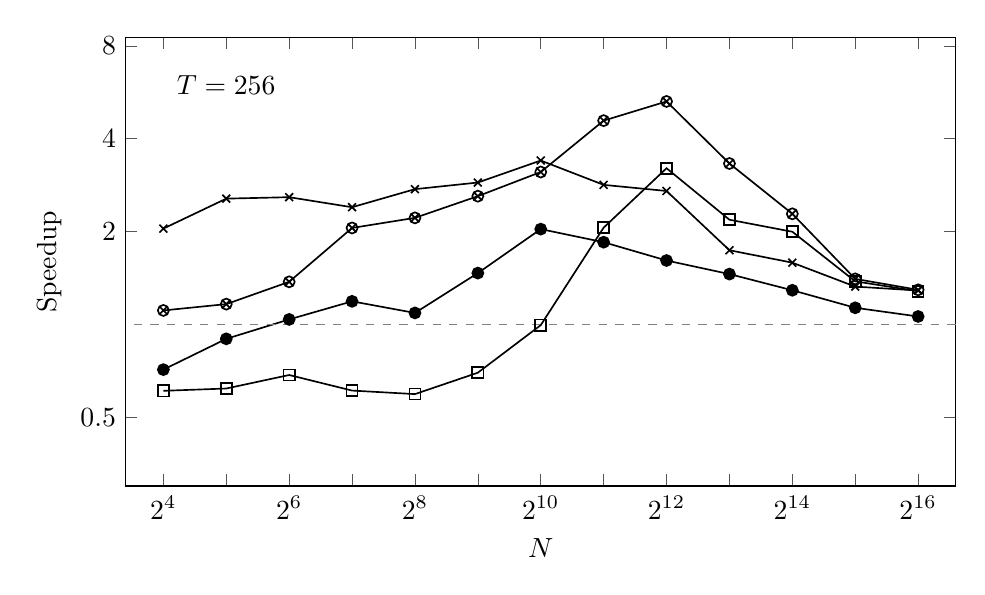
\begin{tikzpicture}

\begin{axis}[
axis line style={black},
xlabel={$N$},
xlabel near ticks,
xmin=-0.6, xmax=12.6,
xtick style={color=white!33.3333333333333!black},
xtick={0,1,2,3,4,5,6,7,8,9,10,11,12},
xticklabels={\(\displaystyle 2^4\),\(\),\(\displaystyle 2^6\),\(\),\(\displaystyle 2^8\),\(\),\(\displaystyle 2^{10}\),\(\),\(\displaystyle 2^{12}\),\(\),\(\displaystyle 2^{14}\),\(\),\(\displaystyle 2^{16}\)},
ylabel={Speedup},
ylabel near ticks,
ytick style={color=white!33.3333333333333!black},
%ytick={0,1,2,3,4,5,6},
%yticklabels={,\(\displaystyle {1.0}\),,\(\displaystyle {3.0}\),,\(\displaystyle {5.0}\),},
%ymin=0.361127455148372, ymax=5.51707532158344,
ymin=0.3, ymax=8.5,
ymode=log,
log basis y={2},
ytick={0.5,2,4,8},
log ticks with fixed point,
width=\textwidth,
height=0.6\textwidth,
title={$T=256$},
title style={below right,at={(0.05,0.9)}}
]
\addplot [semithick, mark=otimes]
table {%
0 1.11147540983607
1 1.16501650165017
2 1.37581699346405
3 2.05629139072848
4 2.21710526315789
5 2.60615384615385
6 3.12078651685393
7 4.57857142857143
8 5.2827140549273
9 3.32571109871723
10 2.28499799438428
11 1.40641665600068
12 1.29619187709406
};
% \addlegendentry{B1}
\addplot [semithick, mark=square]
table {%
0 0.610244988864143
1 0.620842572062084
2 0.686666666666667
3 0.611408199643494
4 0.595488721804511
5 0.698653198653199
6 0.995929443690638
7 2.06111111111111
8 3.21023359288098
9 2.18633540372671
10 1.99912018300194
11 1.38082448735985
12 1.28262231666122
};
% \addlegendentry{B2}
\addplot [semithick, mark=x]
table {%
0 2.04658385093168
1 2.55905511811024
2 2.58680555555556
3 2.4
4 2.74642857142857
5 2.88562091503268
6 3.40054495912806
7 2.83580080753701
8 2.70911949685535
9 1.74132043255549
10 1.58726097495287
11 1.32766260484254
12 1.2893861343636
};
% \addlegendentry{B3}
\addplot [semithick, mark=*]
table {%
0 0.714707329070339
1 0.899248120300752
2 1.03947368421053
3 1.18948412698413
4 1.09095002251238
5 1.46853146853147
6 2.03842794759825
7 1.84909727836163
8 1.61319515399212
9 1.45761636107193
10 1.29182463005992
11 1.13366620453858
12 1.06254475718846
};
% \addlegendentry{B4}
\addplot[gray, dashed] coordinates {(-1,1) (13,1)};
\end{axis}

\end{tikzpicture}
}}
\subfloat[]{\resizebox{0.45\textwidth}{!}{% This file was created by tikzplotlib v0.9.2.
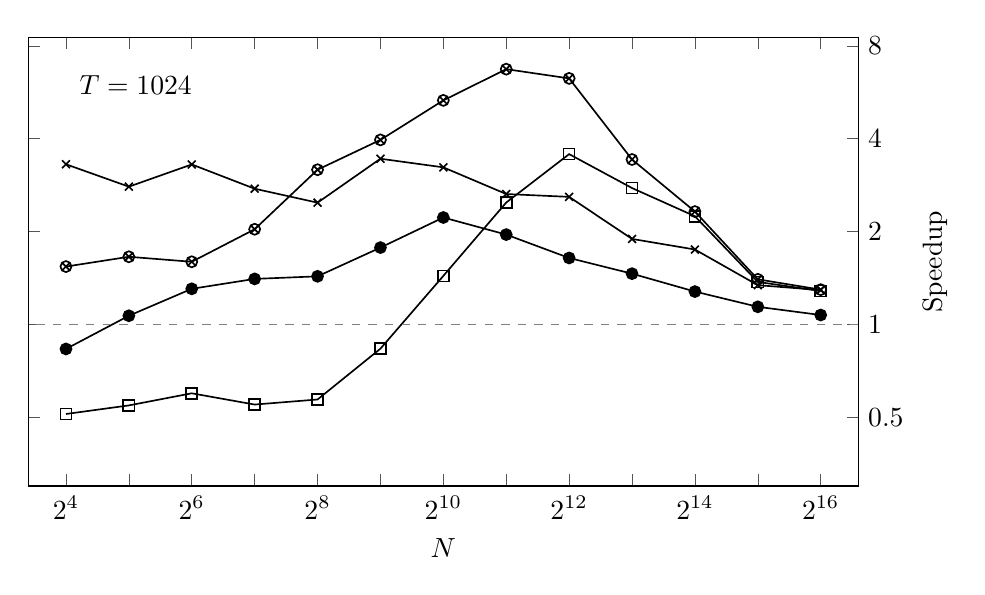
\begin{tikzpicture}

\begin{axis}[
axis line style={black},
xlabel={$N$},
xmin=-0.6, xmax=12.6,
xlabel near ticks,
xtick style={color=white!33.3333333333333!black},
xtick={0,1,2,3,4,5,6,7,8,9,10,11,12},
xticklabels={\(\displaystyle 2^4\),\(\),\(\displaystyle 2^6\),\(\),\(\displaystyle 2^8\),\(\),\(\displaystyle 2^{10}\),\(\),\(\displaystyle 2^{12}\),\(\),\(\displaystyle 2^{14}\),\(\),\(\displaystyle 2^{16}\)},
ylabel={Speedup},
ylabel near ticks,
%ymin=0.202966825333382, ymax=7.6,
ytick style={color=white!33.3333333333333!black},
%yticklabels={,\(\displaystyle {1.0}\),,\(\displaystyle {3.0}\),,\(\displaystyle {5.0}\),,\(\displaystyle {7.0}\),\(\displaystyle {8.0}\)},
ymode=log,
log basis y={2},
ymin=0.3, ymax=8.5,
ytick={0.5,1,2,4,8},
log ticks with fixed point,
yticklabel pos=right,
width=\textwidth,
height=0.6\textwidth,
title={$T=1024$},
title style={below right,at={(0.05,0.9)}}
]
\addplot [semithick, mark=otimes]
table {%
0 1.54172560113154
1 1.65860215053763
2 1.59782608695652
3 2.03624161073826
4 3.17523056653491
5 3.96593673965937
6 5.32525951557093
7 6.72148541114058
8 6.2743450321305
9 3.42638125542378
10 2.32380177063193
11 1.40163487155345
12 1.29789579295094
};
% \addlegendentry{B1}
\addplot [semithick, mark=square]
table {%
0 0.513372472276582
1 0.547333333333333
2 0.599075297225892
3 0.550828729281768
4 0.57201646090535
5 0.835728952772074
6 1.43811764705882
7 2.48555411815438
8 3.56691152986266
9 2.76931747025673
10 2.24389385867926
11 1.37479676536026
12 1.28436651244046
};
% \addlegendentry{B2}
\addplot [semithick, mark=x]
table {%
0 3.30685203574975
1 2.79770114942529
2 3.30263157894737
3 2.75550891920252
4 2.48282630029441
5 3.44634377967711
6 3.23179190751445
7 2.64840182648402
8 2.59288461538462
9 1.89490421158768
10 1.7509535977484
11 1.34198274819622
12 1.29377530790229
};
% \addlegendentry{B3}
\addplot [semithick, mark=*]
table {%
0 0.833864844343204
1 1.06823060410917
2 1.30601343101343
3 1.40609367894497
4 1.4334323922734
5 1.77639399943391
6 2.22291134622401
7 1.9573504027618
8 1.64384220061375
9 1.46215812497777
10 1.27950960037583
11 1.14186188461619
12 1.07420840134936
};
% \addlegendentry{B4}
\addplot[gray, dashed] coordinates {(-1,1) (13,1)};
\end{axis}

\end{tikzpicture}
}}
\caption[]{Speedup of concurrent execution with hidden helper tasks compared to vanilla LLVM with different benchmarks.}
\label{fig:speedup-nw-vanilla}
\end{figure}

\paragraph{Recent Progress}
In recent work we implemented loop transformation constructions introduced in OpenMP 5.1~\cite{kruse2021openmpbooth,kruse2021clangast}, asynchronous offloading for OpenMP~\cite{thiddenhelper}, efficient lowering of idiomatic OpenMP code to GPUs (under review),  OpenMP-aware compiler optimizations with informative and actionable remarks for users (under review), a portable OpenMP device (=gpu) runtime written in OpenMP 5.1 (including atomic support)~\cite{DBLP:conf/iwomp/TianCDC21}, a virtual GPU as debugging friendly
offloading target on the host~\cite{DBLP:conf/icppw/PatelTDC21}, improved diagnostics and execution information~\cite{DBLP:conf/icppw/DoerfertHC21,DBLP:conf/iwomp/HuberWGDH21}.

We redone the OpenMP GPU code generation in LLVM/Clang~\cite{OpenMPEncoding} to improve performance and correctness.
This work was complemented by a new LLVM/OpenMP GPU device runtime that helps us further close the performance gap compared to CUDA and other kernel languages~\cite{NewOpenMPRT}.
Various efforts in improving development and debugging have also been integrated into LLVM/OpenMP~\cite{DBLP:conf/icppw/DoerfertHC21,DBLP:conf/icppw/PatelTDC21}.

We implemented hidden helper task design in LLVM/OpenMP.
Most of our work \cite{DBLP:conf/iwomp/TianCDC21} (except device side dependence resolution) have been upstream and already part of LLVM since 12.0.
Recently Intel also adopted our design and implementation in Intel's latest OpenMP compiler \cite{TianUpdateOnIntelCompiler2021}.

\begin{figure}[tb]
\centering
\subfloat[][Unrolling on AMD EPIC 7532 CPU]{\includegraphics[width=0.5\textwidth]{projects/2.3.2-Tools/2.3.2.11-SOLLVE/unroll.pdf}}%
\subfloat[][Tiling on Intel i5-9400F CPU compared to chunking]{\includegraphics[width=0.5\textwidth]{projects/2.3.2-Tools/2.3.2.11-SOLLVE/tiling.pdf}}
\caption{Performance impact of loop transformations on CPUs.}
\label{fig:unrolltile}
\end{figure}

The loop transformation constructs implemented in Clang include the unroll and tile directives.
We demonstrate how these make speedup in the vicinity of 3$\times$ (tiling on GPU) and an additional 20\% become
low-hanging fruits by just adding a directive~\cite{kruse2021openmpbooth} as illustrated in \autoref{fig:unrolltile}.
There are actually two implementations, one AST-based and a second using the OpenMPIRBuilder that can also be used other compilers such as Flang~\cite{kruse2021clangast}.

Testing of OpenMP offloading for NVIDIA and AMD GPUs has been added to LLVM's Continuous Integration infrastructure.
This will allow identifying changes that break OpenMP early during development, including those by non-OpenMP developers making maintenance easier.

GPU kernel times have been improved significantly since LLVM 12. \autoref{fig:kernel_times} illustrates the impact of
different optimizations we integrated into LLVM and which are run by default for OpenMP codes. As shown, speedups
of up to 13.35$\times$ (RSBench, upper right) were reached while we get closer to CUDA
performance across the board. More recent improvements caused benchmarks like
XSBench (upper left) to also achieve CUDA performance when compiled with OpenMP
offload via our development branch of LLVM/Clang.

\begin{figure}[hbt!]
\centering
\includegraphics[width=0.95\linewidth]{projects/2.3.2-Tools/2.3.2.11-SOLLVE/LLVM-opt-kernel-times.jpg}
\caption[]{Kernel times for different ECP proxy apps when compiled with OpenMP offloading and CUDA. For the former differently optimized versions are shown and the results of a close to LLVM upstream branch is marked explicitly. All times are normalized against LLVM 12 OpenMP offloading performance.}
\label{fig:kernel_times}
\end{figure}

LLVM/Clang 13.0.0 has been officially released on October 4, 2021, which includes most of the aforementioned improvements. The branch for LLVM/Clang 14.0.0 has been branched-off the development repository and is expected to be released March 15 2022.


\subparagraph{Case study: LLVM/OpenMP performance for OpenMC}

We intensified our work with the OpenMC team on their portable OpenMP implementation of a Monte Carlo code.
Most recent results obtained with LLVM/OpenMP show how our compile enhancements and application engagement improve performance manifold.
Further, the early results on AMD GPUs are very promising and indicate that performance portability is achievable with LLVM/OpenMP.
The performance evolution through our collaboration is summarized in \autoref{fig:openmc}. JLSE testbeds from Argonne National Lab have been used for these results.  
A more detailed report was recently accepted to the PHYSOR conference.


  \definecolor{col0o}{RGB}{0,146,146}
  \colorlet{col0}{col0o!80}
  \definecolor{col1o}{RGB}{182,109,255}
  \colorlet{col1}{col1o!70}
  \definecolor{col2}{RGB}{219,209,0}
  \definecolor{col3}{RGB}{255,182,119}
  \definecolor{col8}{RGB}{182,255,219}
  \definecolor{col5}{RGB}{36,255,36}
  \definecolor{col6}{RGB}{182,219,255}
  \definecolor{col7}{RGB}{255,109,182}
  \definecolor{col18}{RGB}{255,255,109}
  \definecolor{col9}{RGB}{73,0,146}
  \definecolor{col10}{RGB}{146,73,0}
  \definecolor{col11}{RGB}{146,0,0}
  \definecolor{col12}{RGB}{0,109,219}
  \definecolor{col13}{RGB}{0,73,73}
  \definecolor{col14}{RGB}{73,0,73}
  \definecolor{col15}{RGB}{73,73,0}
  \definecolor{col16o}{RGB}{255,36,36}
  \colorlet{col16}{col16o!80}
  \definecolor{col17o}{RGB}{36,36,255}
  \colorlet{col17}{col17o!50}
  \definecolor{col4}{RGB}{255,182,219}
  
  \definecolor{Maroon}{HTML}{990000} 

\begin{figure}[h!]
  \vspace*{3mm}
  \centering

\resizebox{\linewidth}{!}{%
  %\includegraphics{includes/openmc.pdf}

\begin{tikzpicture}
\begin{axis}[
    compat=newest,
    enlarge y limits={rel=0.20},
    enlarge x limits={abs=0.5},
    ybar,
    ymode = log,
    log basis y = 10,
    bar width=40,
    xtick={1,2,3,4,5},
    xticklabels={CPU\\32 cores, A100 initial\\ performance, A100 after application-\\compiler co-design\\ (OpenMC + LLVM), A100 after further\\ algorithmic changes\\ (OpenMC team), AMD MI100 perf-\\ormance latest\\ OpenMC + LLVM},
    xtick style={draw=none},
    xticklabel style={align=center,font=\small},
    %xmajorticks=false,
    ymajorgrids=true,
    ylabel={particles/sec},
    %ylabel style = {align=center,at={(-0.08,0.5)}},
    %yminorgrids=true,
    grid style=dashed,
    height=7cm,
    width=18cm,
    visualization depends on ={y \as \y},
    visualization depends on ={rawy \as \rawy},
    %log ticks with fixed point,
    every node near coord/.append style = {
      %name=a\coordindex,
      %font=\small,
      /pgf/number format/fixed,
      %fill=white,
      %yshift=-2pt,
      %inner sep=0pt,
    },
    every axis plot/.append style={
      bar shift=0pt,
    },
  ]
\addplot[
    %nodes near coords,
    %point meta=rawy,
    nodes near coords={%
      \begingroup%
        % this group is merely to switch to FPU locally.
        % Might be unnecessary, but who knows.
        \pgfkeys{/pgf/fpu}%
        \pgfmathparse{\pgfplotspointmeta<4}%
        \global\let\issmall=\pgfmathresult%
        \pgfmathparse{\pgfplotspointmeta==0}%
        \global\let\iszero=\pgfmathresult%
        \pgfmathparse{\pgfplotspointmeta==1}%
        \global\let\isone=\pgfmathresult%
      \endgroup%
      \pgfmathfloatcreate{0}{0.0}{0}%
      \let\ZERO=\pgfmathresult%
      \pgfmathfloatcreate{1}{1.0}{0}%
      \let\ONE=\pgfmathresult%
      \color{black}%
      \ifx\iszero\ONE%
      {%
        \hspace*{-5mm}%
        \global\let\ycoord=\ZERO%
        \textbf{OoM}%
      }%
      \else%
        \ifx\isone\ONE%
        {%
          \textbf{base}
          \global\let\ycoord=\ZERO%
        }%
        \else%
          \ifx\issmall\ONE%
          {%
            %\global\let\ycoord=\ZERO
            \textbf{\phantom{,}\pgfmathprintnumber[precision=2]{\rawy}\phantom{,}}%
          }%
          \else%
            %\hspace*{-12mm}
            %\hspace*{-4mm}
            %\global\let\ycoord=\rawy
            %\colorbox{white}{%
              \textbf{\pgfmathprintnumber[precision=2]{\rawy}}%
            %}
          \fi%
        \fi%
      \fi%
    },
    every node near coord/.append style = {
        name=a\coordindex,
        /pgf/number format/fixed,
        yshift=0.5pt,
        fill=white,
        inner sep=0pt,
    },
    fill=Maroon,
  ]
  coordinates {
(2,602)
(3,58529)
(4,349685)
};

\addplot[
    %nodes near coords,
    %point meta=rawy,
    nodes near coords={%
      \begingroup%
        % this group is merely to switch to FPU locally.
        % Might be unnecessary, but who knows.
        \pgfkeys{/pgf/fpu}%
        \pgfmathparse{\pgfplotspointmeta<4}%
        \global\let\issmall=\pgfmathresult%
        \pgfmathparse{\pgfplotspointmeta==0}%
        \global\let\iszero=\pgfmathresult%
        \pgfmathparse{\pgfplotspointmeta==1}%
        \global\let\isone=\pgfmathresult%
      \endgroup%
      \pgfmathfloatcreate{0}{0.0}{0}%
      \let\ZERO=\pgfmathresult%
      \pgfmathfloatcreate{1}{1.0}{0}%
      \let\ONE=\pgfmathresult%
      \color{black}%
      \ifx\iszero\ONE%
      {%
        \hspace*{-5mm}%
        \global\let\ycoord=\ZERO%
        \textbf{OoM}%
      }%
      \else%
        \ifx\isone\ONE%
        {%
          \textbf{base}
          \global\let\ycoord=\ZERO%
        }%
        \else%
          \ifx\issmall\ONE%
          {%
            %\global\let\ycoord=\ZERO
            \textbf{\phantom{,}\pgfmathprintnumber[precision=2]{\rawy}\phantom{,}}%
          }%
          \else%
            %\hspace*{-12mm}
            %\hspace*{-4mm}
            %\global\let\ycoord=\rawy
            %\colorbox{white}{%
              \textbf{\pgfmathprintnumber[precision=2]{\rawy}}%
            %}
          \fi%
        \fi%
      \fi%
    },
    every node near coord/.append style={
        /pgf/number format/fixed,
        yshift=0.5pt,
        fill=white,
        inner sep=0pt,
    },
    fill=col6,
  ]
  coordinates {
(1,54913)
};
\addplot[
    %nodes near coords,
    %point meta=rawy,
    nodes near coords={%
      \begingroup%
        % this group is merely to switch to FPU locally.
        % Might be unnecessary, but who knows.
        \pgfkeys{/pgf/fpu}%
        \pgfmathparse{\pgfplotspointmeta<4}%
        \global\let\issmall=\pgfmathresult%
        \pgfmathparse{\pgfplotspointmeta==0}%
        \global\let\iszero=\pgfmathresult%
        \pgfmathparse{\pgfplotspointmeta==1}%
        \global\let\isone=\pgfmathresult%
      \endgroup%
      \pgfmathfloatcreate{0}{0.0}{0}%
      \let\ZERO=\pgfmathresult%
      \pgfmathfloatcreate{1}{1.0}{0}%
      \let\ONE=\pgfmathresult%
      \color{black}%
      \ifx\iszero\ONE%
      {%
        \hspace*{-5mm}%
        \global\let\ycoord=\ZERO%
        \textbf{OoM}%
      }%
      \else%
        \ifx\isone\ONE%
        {%
          \textbf{base}
          \global\let\ycoord=\ZERO%
        }%
        \else%
          \ifx\issmall\ONE%
          {%
            %\global\let\ycoord=\ZERO
            \textbf{\phantom{,}\pgfmathprintnumber[precision=2]{\rawy}\phantom{,}}%
          }%
          \else%
            %\hspace*{-12mm}
            %\hspace*{-4mm}
            %\global\let\ycoord=\rawy
            %\colorbox{white}{%
              \textbf{\pgfmathprintnumber[precision=2]{\rawy}}%
            %}
          \fi%
        \fi%
      \fi%
    },
    every node near coord/.append style={
        /pgf/number format/fixed,
        yshift=0.5pt,
        fill=white,
        inner sep=0pt,
    },
    fill=col3,
  ]
  coordinates {
  (5,93918)
};
\end{axis}

\draw[ultra thick,->,shorten <=1mm,shorten >=3mm] ($(a0.south east) + (3mm,0mm)$) -- node[midway,above,rotate=55,fill=white,inner sep=1pt,yshift=2pt] {97x} ($(a1.south west) + (-0.5mm,1mm)$);
\draw[ultra thick,->,shorten <=1mm,shorten >=3mm] ($(a1.south east) + (3mm,0mm)$) -- node[midway,above,rotate=30,fill=white,inner sep=1pt,yshift=2pt] {6x} (a2.south west);

\end{tikzpicture}
}

\vspace*{-2mm}

\caption{
  Performance results for the OpenMC~\cite{romano2013openmc} OpenMP offloading code that simulates transport of neutral particles using the Monte Carlo methodology.
  The application is part of the ExaSMR ECP project and known for its proxy applications (XSBench~\cite{XS_Tramm_2014} and RSBench~\cite{RS_Tramm_2014}).
  Results show the almost 100x speedup achieved by co-optimizing the full OpenMC application with the LLVM compiler for OpenMP offloading on NVIDIA A100 GPUs.
  In the process, changes to both OpenMC and LLVM were made, and the latter were often triggered via command line options or assumptions.
  Guided by compiler remarks, other applications could benefit similarly and with far less involvement from a compiler developer---but only if the remarks, and later the suggested code changes, are clear, actionable, and effective.
 For context, we also present the AMD MI100 numbers obtained with the latest versions
 of OpenMC and the LLVM/Clang compiler.
 Since the LLVM/OpenMP offloading backend for AMD GPU is new and only recently became stable, we expect substantial performance improvements as we start our tuning efforts.
 Even without, we believe the results shows how performance portability is certainly
 within reach for a full application using the LLVM/OpenMP offloading environment. \\
  The data for the figure was generated and generously provided by John Tramm.
}

  \label{fig:openmc}
  %\vspace*{-2mm}
  \vspace*{2mm}
\end{figure}


\paragraph{Next Steps}
We will keep working on supporting more new OpenMP 5.1 features in LLVM.
%OpenMP 5.1 introduces a number of new features, one of which is new set of useful atomic operations, \texttt{compare} clause and a combined one \texttt{compare capture}.
%Now most of atomic operations in scientific applications can be written in OpenMP directly instead of using target dependent intrinsics or function calls.
%We will support the two clauses in LLVM/Clang.
%
To avoid redundant development of two OpenMP implementations, we will mature the development of the OpenMPIRBuilder and make it the default OpenMP code generation for Clang as it is already for Flang.

Improvements to the OpenMP offloading ecosystem are planned, e.g., to extend the remote offloading capabilities we introduced and to further improve development and debugging of OpenMP GPU applications.

More OpenMP-aware optimizations are expected to materialize as we get the last OpenMP benchmarks on par with CUDA performance. We also plan to invest time in generic GPU optimizations soon.

We will implement proof-of-concept implementations of loop transformations that are planned for OpenMP 6.0, such as loop interchange, reversal, fusion, fission and index set splitting.


\paragraph{Experiences on Early Access Systems}

%The SOLLVE team has implemented and optimized an OpenMP offload version of AutoDock-GPU based on a OpenMP CPU OpenMP tasking version, 

AutoDock-GPU is an application code for molecular docking often used to solve problems in the domains of biology and AI/ML on supercomputers including DoE's supercomputers, and it has recently (in 2020 and 2021) been used as the driver for simulations run on supercomputers for developing COVID-19 therapeutics~\cite{legrand2020gpu}. AutoDock-GPU uses OpenMP offload features to run on a single GPU and has the ability for parallelize and schedule computation across multiple GPUs on a node through OpenMP. The OpenMP offload implementation of AutoDock-GPU was developed by members of the SOLLVE team. The application code has been experimented with using LLVM 12 OpenMP and LLVM 13 OpenMP on one node of the Spock Early Access System provided by ECP. Note that the LLVM 13 results were not in our SOLLVE FY21 Program Review slides and we only showed LLVM 12 then.

Figure~\ref{fig:llvmadspck} shows the wall clock timings of AutoDock-GPU when using 3 different sizes of ligands on one GPU of Spock, under LLVM OpenMP 12 and LLVM OpenMP 13. The results show that LLVM 13 OpenMP (rocm4.5) improves performance over LLVM 12 OpenMP (rocm4.2) of the AutoDock-GPU for the largest problem size, i.e., the 3er5 ligand, by 16.56\%. The results show that the LLVM OpenMP implementation version generally has an impact to performance and suggests has a larger impact with larger problem size for this application. 

\begin{figure}[h!]
    \centering
    \subfloat[One GPU. \label{fig:llvmadspck}] {\includegraphics[scale=0.5]{projects/2.3.2-Tools/2.3.2.11-SOLLVE/one_gpu_spock.png}}\subfloat[One node (four GPUs). \label{fig:mgpuSpock} ]{\includegraphics[scale=0.5]{projects/2.3.2-Tools/2.3.2.11-SOLLVE/multi_gpu_spock.png}}
    \caption{Running AutoDock-GPU with LLVM's OpenMP on Spock.} 
\end{figure}

Figure~\ref{fig:mgpuSpock} shows results for strategies for an OpenMP parallelization of AutoDock-GPU (using an assortment of the three ligands in Figure~\ref{fig:llvmadspck}) across the 4 GPUs of Spock. The figure specifically shows the difference in performance between a static assignment of the application's computation to GPUs and a dynamic assignment - or scheduling - of the application's computation across multiple GPUs of the node, as discussed in~\cite{9669317}, and the impact of the LLVM OpenMP implementation version. The round-robin scheduler under LLVM 13 OpenMP (rocm4.5) improves performance over the round-robin scheduler in LLVM 12 OpenMP (rocm4.2) by 10.73\%. Under LLVM 13’s OpenMP (rocm4.5), using a dynamic assignment (labeled \textit{random} in Figure~\ref{fig:mgpuSpock} and where OpenMP chunks of a loop are assigned to randomly chosen GPU) as opposed to a static assignment (labeled \textit{round-robin} in Figure~\ref{fig:mgpuSpock} and where OpenMP chunks are assigned to a GPU based on chunk number) cuts the execution time by 45.63\%. By using the newer LLVM 13 over LLVM 12 and by using the random multiGPU scheduling strategy instead of the round-robin scheduling strategy, AutoDock-GPU is sped up by approximately 2.05$\times$. Using the dynamic multiGPU scheduling strategy over the static one improves performance 4.5$\times$ more than using the new LLVM OpenMP implementation version over the older one, but the newer LLVM OpenMP implementation version still helps improve performance substantially and by about 10\%. 

\subsubsection{\stid{2.11} Building tools to detect and debug bugs and performance issues with OMP offloading}

\paragraph{Overview}
Starting from the 4.0 version, OpenMP has introduced a new feature, \textit{target offloading}, which enables programmers to leverage additional computing ``devices'' connected to the host (e.g., GPU, application-specific accelerator).
With a group of hardware-agnostic constructs (\textit{device directives}), target offloading makes it possible to write accelerated OpenMP applications in a performance-portable manner. However, concurrency bugs and performance issues may still arise due to  incorrect usage of device directives. 
Our group at Georgia Tech has conducted a comprehensive study of such issues~\cite{yu2020study}. We found that most of these issues are related to the data mappings between the host and target device.
For example, incorrect data mappings can lead to uninitialized memory accesses or even buffer overflow on the target device. In addition, programmers may also declare data mappings that incur unnecessary time and memory overhead due to redundant copies.

To help programmers detect and debug these concurrency bugs and performance issues, we have developed a toolset for OpenMP applications including:
\begin{itemize}
    \item OMPSan~\cite{barua2019ompsan}, a static analyzer that can report all suspicious data mappings that may lead to concurrency bugs and memory issues;
    \item ARBALEST~\cite{yu2021arbalest}, a dynamic analyzer that can pinpoint incorrect data mappings that result in concurrency bugs or memory issues at runtime;
    \item OmpMemOpt~\cite{barua2020ompmemopt}, a static optimizer identifies redundant data mappings and replaces them by more optimized data mappings.
\end{itemize}

\paragraph{Key Challenges}
With respect to incorrect data mappings, multiple kinds of bugs may arise at runtime, such as use of uninitialized memory, use of stale data, buffer overflow, and data race. Currently, there exists no tool that can recognize all these bugs' behavior. 
Even if programmers apply multiple analysis tools when testing a single OpenMP application, some incorrect data mappings may still be missed since they may only trigger bugs in a specific thread interleaving.
On the other hand, detecting redundant data mappings may also be challenging. OpenMP utilizes a reference-count algorithm to manage the lifecycle of each data mapping. Memory transfer is only carried out when a data mapping is first encountered.
The analysis tool needs to correctly model this reference-count-based mechanism and all memory accesses related to data mappings to determine whether a data mapping is redundant.

\paragraph{Solution Strategy}
As a static analysis tool, OMPSan~\cite{barua2019ompsan} compares the def-use information in an OpenMP application with the application's serial-elision version. OMPSan assumes that the serial-elision version contains the correct def-use information. Any inconsistent def-use chain incurred by data mappings can be statically reported as a potential bug.

ARBALEST is a dynamic analysis tool designed for incorrect data mappings. It is an extension to the Archer data race detector~\cite{atzeni2016archer}. ARBALEST leverages a state-transition diagram to record the state of each data mapping, i.e., whether the memory section on the host/target device has a valid value. ARBALEST also utilizes the happens-before relations maintained by Archer to detect conflicting memory accesses when the runtime conducts memory transfer for a data mapping.
According to the evaluation in~\cite{yu2021arbalest}, ARBALEST can accurately identify all incorrect data mappings with acceptable time and memory overhead.

OmpMemOpt\cite{barua2020ompmemopt} is a static optimizer that can generate optimal data mappings for an OpenMP application. 
The optimization framework in OmpMemOpt casts the problem of detection and removal of redundant data movements into a partial redundancy elimination (PRE) problem and applies
the lazy code motion technique to optimize these data movements.
The evaluation on ten benchmarks shows that OmpMemOpt achieved a geometric speedup of 2.3×, and reduced on average 50\% of the total bytes transferred between the host and GPU.

\paragraph{Recent Progress}
We have achieved a number of publications for the toolset. OMPSan has been presented at IWOMP 2019 and was selected as the best paper award recipient in that two workshops. The other two papers on ARBALEST and OmpMemOpt were presented at IPDPS 2021 and Euro-Par 2020 respectively.

\paragraph{Next Steps}
We are working with the LLVM OpenMP subcommunity to develop a new version of ARBALEST. The new implementation will be built on the latest LLVM and apply a number of optimization techniques to reduce the time overhead. Besides, we are also helping improve the OpenMP Tool Interface design based on our experience of developing analysis tools.
\subsubsection{\stid{2.11}Validation and Verification Testsuite}

\paragraph{Overview}
The OpenMP Validation and Verification Testsuite (OMPVV) presents the community with a test suite comprised of functional tests and application kernels that are written with the intention of verifying usability of OpenMP features. The test suite aims to accomplish several goals of equal importance. The first goal is to provide vendors with a straightforward way to examine the status of their implementations. The next goal is to support application developers in identifying whether their system can support the specific OpenMP features they wish to utilize. Both of these are accomplished by running the full test suite and generating a report summary, which provides the user with a simple pass-fail report for OpenMP features. These insights also include where the tests are failing (compile time or runtime) and what is the error encountered. Our full suite of OpenMP tests is made publicly available on Github \cite{sollvevvgithub} and full documentation in available the corresponding website \cite{sollvevvwebsite}. 

\paragraph{Key Challenges}
Every few years, the OpenMP Architecture Review Board releases new versions of their specification. These new releases of the specification, 5.0 in November of 2018 and 5.1 in November of 2020, introduce new clauses and directives that many application developers and general users are keen on utilizing. Thus, when the updates are published, we set out to create tests for each new feature or new directive. It takes time for the compiler developers to develop implementations for several of the new features, as a result there is a gap between versions released by the specification, implementations developed and implementations made available for the application developers. Due to this fact, we are often times writing test cases for new clauses and directives even before the implementations begin to exist. This can be quite a challenge since we cannot even compile or execute them right away, so would need to revisit the test cases as soon as the implementations are made available. 

\paragraph{Solution Strategy}
 When OpenMP 5.0 was released in 2018, we began by identifying all of the features reported to be 'implemented' or 'partially implemented' by LLVM's OpenMP implementation status page and placed those tests at the top of our priority list. Additionally, we identified the features that were of great importance to application developers and also associated these as 'high priority' tests. Since the release of OpenMP 5.1 in 2020, we have adopted the same strategy as before. As more features are implemented by LLVM, we continue to create functional tests cases and verify our own work by running the tests on several heterogeneous systems that represent multiple vendors and OpenMP compiler implementations. In previous years, we followed the same strategy for providing OpenMP 4.5 test coverage \cite{vandv2019}.

\paragraph{Recent Progress}
Over the past year, we have been able to provide tests (C, C++, and Fortran90) that cover almost all of the new features introduced in OpenMP 5.0. We have continued to report the pass-fail status and individual test results on state-of-the-art systems such as Oak Ridge National Lab's Summit and Spock computing systems as well as NERSC's Cori system. Also, we have created functional tests for several of the latest OpenMP 5.1 features that have been implemented by LLVM and deemed of high importance to application developers.

\paragraph{Next Steps}
Following the release of the OpenMP 5.1 specification, we have continued to follow the same strategy as we did for providing test coverage of 5.0 features. As LLVM continues to make progress implementing the new 5.1 features, we will continue to generate new functional tests and run our tests on the newest available compiler implementations that support OpenMP.  Additionally, we have a list of features that application developers are interested in using and will consult this list as a priority list alongside the LLVM implementation status list. 
\subsubsection{\stid{2.11} Training \& Outreach in 2021}\label{subsubsect:train_outreach}

\begin{enumerate}
\item Annual ECP Meeting 2021 related
\begin{itemize}
    \item \enquote{OpenMP Tutorial} by O. Hernandez, D. Oryspayev, T. Scogland, C. Bertoni, J. Doerfert, and V. Kale
    \item \enquote{ECP + SOLLVE COVID} 
    \item \enquote{OpenMP Application Experiences BoF} 
    \item \enquote{LLVM in ECP Short Stories About a Compiler Framework in HPC} 
    \item \enquote{OpenMP Vendor BoF}
    \item \enquote{Session on Testing in ECP including OpenMP V\&V Suite} 
    \item \enquote{Tutorial: Autotuning PolyBench Benchmarks with LLVM Clang/Polly Loop Optimization Pragmas Using Bayesian Optimization}
\end{itemize}

\item \enquote{OpenMP Users Monthly Telecons\footnote{\url{https://www.openmp.org/events/ecp-sollve-openmp-monthly-teleconference/}}} led by D. Oryspayev

\item Weekly \enquote{OpenMP-in-LLVM} teleconference with DOE labs and vendors (AMD, Intel, Cray, ...)

\item Biweekly \enquote{OpenMP work in Flang} teleconference with DOE labs and vendors (AMD, ARM, NVIDIA, ...)

\item Hackathons

\begin{itemize}
    \item \enquote{ECP SOLLVE + NERSC OpenMP Hackathon\footnote{\url{https://sites.google.com/view/ecpomphackjan2021/home}}}, January 22, and 27 – 29, 2021
    \begin{itemize}
        \item Organizers: C. Daley, D. Oryspayev, K. Gott, H. He, O. Hernandez, and V. Kale 
    \end{itemize}
    \item \enquote{ECP OpenMP Virtual Hackathon\footnote{\url{https://www.bnl.gov/ompbrookathon2021/}}}, October 1, and 6 -8, 2021
    \begin{itemize}
        \item Organizers: D. Oryspayev, J. Doerfert, S. Chandrasekaran, S. Pophale, T. Scogland, and V. Kale  
    \end{itemize}
\end{itemize}

\item ISC HPC'21\footnote{\url{https://www.isc-hpc.com/schedule.html}} related tutorials \& presentations
\begin{itemize}
    \item Tutorial: \enquote{OpenMP Common Core: Learning Parallelization of Real Applications from the Ground-Up} by M. Arenaz, B. Chapman, R. Budiardja, O. Hernandez, and D. Oryspayev.
\end{itemize}

\item OpenMP.org Webinars 
\begin{itemize}
    \item \enquote{A Compiler's View of the OpenMP API\footnote{\url{https://www.openmp.org/events/webinar-a-compilers-view-of-the-openmp-api/}}} by J. Doerfert.
    \item \enquote{The Leaders of OpenMP Discuss the Future of the OpenMP API\footnote{\url{https://www.openmp.org/events/webinar-the-leaders-of-openmp-discuss-the-future-of-the-openmp-api/}}} by M. Klemm and B. de Supinski.
\end{itemize}

\item \enquote{Introduction to OpenMP GPU Offloading\footnote{\url{https://www.olcf.ornl.gov/calendar/introduction-to-openmp-gpu-offloading/}}} by S. Parete-Koon \& S. Pophale, September 22 - 23, 2021
   
\item ICPP'21 presentations:
\begin{itemize}
    \item \enquote{Loop Transformations Using Clang’s Abstract Syntax Tree}, LLVM in Parallel Processing Workshop, by M. Kruse
\end{itemize}
      
\item SC'21\footnote{\url{https://sc21.supercomputing.org/program/}}
\begin{itemize}
    \item OpenMP Tutorials
    \begin{itemize}
        \item \enquote{Advanced OpenMP: Host Performance and 5.1 Features} by C. Terboven, M. Klemm, R. van der Pas, B. R. de Supinski
    \end{itemize}
    \item OpenMP BoF
    \begin{itemize}
        \item \enquote{OpenMP Offloading and the 5.2 API} session led by J. Doerfert and M. Klemm 
    \end{itemize}
    \item OpenMP Booth Talks
    \begin{itemize}
        \item \enquote{Behind the Pragmas} by J. Doerfert
        \item \enquote{Low-overhead Loop Scheduling in OpenMP} by V. Kale
        \item \enquote{Using OpenMP Loop Transformations with Clang} by M. Kruse
        \item \enquote{SOLLVE Validation and Verification Suite} by S. Pophale
    \end{itemize}
    \item Workshops
    \begin{itemize}
        \item \enquote{Loop Transformations Using Clang’s Abstract Syntax Tree}, LLVM-in-HPC Workshop, by M. Kruse
    \end{itemize}
\end{itemize}


\end{enumerate} 
    
      

     

 
\newpage
[\subsubsection{\stid{2.12} Flang}\label{subsubsect:flang}

\paragraph{Overview}

The Flang project provides an open-source Fortran standard 
\cite{iso-fortran-2004, iso-fortran-2010, iso-fortran-2018}
compiler front-end for the LLVM Compiler Infrastructure (see
\url{http://llvm.org})~\cite{llvm:homepage}.  Flang was formally
accepted as an official component of LLVM in 2019 and merged portions
of its initial code base into the main LLVM repository in April 2020. 
Work continues today with a growing set of contributors to the
code base.  Leveraging LLVM, Flang will provide a
cross-platform Fortran solution available to ECP and the broader
international LLVM community. The goals of the project include
extending support to GPU accelerators and target Exascale systems, and
supporting LLVM-based software and tools of interest to a large
deployed base of Fortran applications.

LLVM's growing popularity and wide adoption make it an integral part
of the modern software ecosystem. Flang will provide a foundation
for Fortran that will complement and interoperate with the
Clang C/C++ compiler and other tools within the LLVM infrastructure.
We aim to provide a modern, open-source Fortran implementation that is
stable, has an active footprint within the LLVM community, and will
meet the specific needs of ECP as well as the broader scientific
computing community.

\paragraph{Key Challenges}
Today there are several commercially-supported Fortran compilers,
typically available from one vendor and often for a limited set of
platforms.  None of these are open source.  While the GNU gfortran compiler is
open source and available on a wide variety of platforms, the source base is not modern
LLVM-style C++ and the GPL license is not compatible with
LLVM.  This places limits on a wide breath of potential collaborations, and thus has an
impact on broader community participation and adoption.

The primary challenge of this project is to create a source base with
the maturity, features, and performance of proprietary solutions with
the cross-platform capability of GNU compilers, and which is licensed
and coded in a style that will be embraced by the LLVM community. 
Additional challenges come from supporting all Fortran
language features, language extensions (e.g., OpenMP, OpenACC), and
scalability required for effective use of exascale-class systems. 

\paragraph{Solution Strategy}

With the adoption of Flang into the LLVM community, our strategy
focuses on establishing and growing a strong community around it and the development
and delivery of a solid, alternative Fortran compiler for DOE's
platforms.  It is critical that we be good shepherds within
the LLVM community to successfully establish this community for Flang.
This external engagement is in the best interest
of ECP as well as the long-term success of Fortran, and enables leveraging
the significant momentum and strengths of this widely used and accepted
code base. 

Our path to success will rely on significant testing across not only
the various facilities but also across a very broad and diverse set of
applications. Given the early development stage of Flang, this testing
will be paramount in the delivery of a robust infrastructure to ECP
and the broader community.

\paragraph{Recent Progress}

After several years of effort and support from NNSA, Flang was 
successfully \emph{``adopted''} by the LLVM community and has transitioned 
from a stand-alone git repository to one hosted by the main LLVM project.  This 
represents a significant result and the community reviewed and accepted code is
available via GitHub:

\begin{center}
\url{https://github.com/llvm/llvm-project/}
\end{center}

The current capabilities of Flang include the parsing and semantic
analysis of the full Fortran 2018 standard and OpenMP 5.X. As part of the
development of the parsing and semantic analysis portions of the
front-end, over five million lines of Fortran code have been
successfully processed. Beyond parsing and semantics, we have been
focusing our efforts on creating a Fortran-centric intermediate
representation (Fortran IR -- ``FIR'') that leverages recent activities
within Google on 
\href{Multi-Level Intermediate Representations} 
{https://www.blog.google/technology/ai/mlir-accelerating-ai-open-source-infrastructure/}
(MLIR) for use with the implementation of FIR.
With the development of FIR progressing, we have completed
the first full (sequential) compiler with the full set of F77 
capabilities, and will soon complete the full set of F95 capabilities.
Implementations of the later standards will follow in chronological order.

\paragraph{Next Steps}
Our short-term priorities are focused on up-streaming of the
sequential compiler with Fortran 95 support, completing implementation of the remaining Fortran standards,
the creation of a significant testing infrastructure, and helping to play a key role in
the interactions and overall discussions within the LLVM community.  Longer term efforts
will shift to support OpenMP 5.X features critical to ECP applications
on the target Exascale platforms.  We are actively exploring finding a
common leverage point between Clang's current OpenMP code base and
Flang.  This would enable the reuse of existing code versus writing
everything from scratch in Flang.  We see this as a critical path
forward to enabling a timely release of a node-level parallelizing
compiler for ECP.  Additional work will focus on features that would
benefit Fortran within the LLVM infrastructure as well as general and
targeted optimization and analysis capabilities.


\newpage


%\subsection{\mathlibs}
%This section presents projects in \mathlibs.
\subsection{\stid{3} \mathlibs}\label{subsect:mathlibs}

\textbf{End State:} Mathematical libraries that (i) interoperate with the ECP software stack; (ii) are incorporated into the ECP applications; and (iii) provide scalable, resilient numerical algorithms that facilitate efficient simulations on Exascale computers.

\subsubsection{Scope and Requirements}
Software libraries are powerful means of sharing verified, optimized algorithms and their implementations. Applied research, development, and support are needed to extend existing DOE mathematical software libraries to make better use of Exascale architectural features. DOE-supported libraries encapsulate the latest results from mathematics and computer science R\&D; many DOE mission-critical applications rely on these numerical libraries and frameworks to incorporate the most advanced technologies available. 

The Mathematical Libraries effort will ensure the healthy functionality of the numerical software libraries on which the ECP applications will depend. The DOE mathematical software libraries used by computational science and engineering applications span the range from light-weight collections of subroutines with simple APIs to more “end-to-end” integrated environments and provide access to a wide range of algorithms for complex problems.

Advances in mathematical and scientific libraries will be necessary to enable computational science on Exascale systems. Exascale computing promises not only to provide more computational resources enabling higher-fidelity simulations and more demanding studies but also to enable the community to pose new scientific questions. Exascale architectural characteristics introduce new features that algorithms and their implementations will need to address in order to be scalable, efficient, and robust. As a result, it will be necessary to conduct research and development to rethink, reformulate, and develop existing and new methods and deploy them in libraries that can be used by applications to deliver more complete and sophisticated models and provide enhanced predictive simulation and analysis capabilities.

The Mathematical Libraries effort must (1) collaborate closely with the Application Development effort (WBS 2.2) to be responsive to the needs of the applications and (2) collaborate with the other products within the Software Technology effort (WBS 2.3) in order to incorporate new technologies and to provide requirements. All software developed within the Mathematical Libraries effort must conform to best practices in software engineering, which will be formulated early in the project in collaboration with the Applications Development focus area. Software produced by this effort must provide scalable numerical algorithms that enable the application efforts to reach their performance goals, encapsulated in libraries whose data structures and routines can be used to build application software.

\subsubsection{Assumptions and Feasibility}
Years of DOE investment have led to a diverse and complementary collection of mathematical software, including AMReX, Chombo, hypre, Dakota, DTK, MAGMA, MFEM, PETSc/TAO, PLASMA, ScaLAPACK, SUNDIALS, SuperLU, and Trilinos. This effort is evolving a subset of existing libraries to be performant on Exascale architectures. In addition, research and development is needed into new algorithms whose benefits may be seen only at the extreme scale. Results of preliminary R\&D projects indicate that this approach is feasible.

Additionally, ECP will need to rely on a strong, diverse, and persistent base math research program, which is assumed to continue being supported by the DOE-SC ASCR Office. The ECP technical directors will schedule quarterly meetings with the ASCR research program managers to get updates on research results that might meet ECP requirements as well as to inform the program managers of ECP needs in applications and software components.

\subsubsection{Objectives}
The high-level objective of the Mathematical Libraries effort is to provide scalable, resilient numerical algorithms that facilitate efficient application simulations on Exascale computers. To the greatest extent possible, this objective should be accomplished by preserving the existing capabilities in mathematical software while evolving the implementations to run effectively on the Exascale systems and adding new capabilities that may be needed by Exascale applications.

The key performance metrics for the software developed by this effort are scalability, efficiency, and resilience. As a result of the new capabilities in mathematics libraries developed under this effort, applications will tackle problems that were previously intractable and will model phenomena in physical regimes that were previously unreachable.

\subsubsection{Plan}
As detailed below, the Mathematical Libraries effort supports six complementary L4 projects as needed to meet the needs of ECP applications. These efforts include strong collaborations among DOE labs, academia, industry, and other organizations, and leveraging existing libraries that are widely used by the DOE HPC community. 

Initial efforts have focused on identifying core capabilities needed by selected ECP applications, establishing performance baselines of existing implementations on available Petascale and prototype systems, and beginning re-implementation of lower-level capabilities of the libraries and frameworks. Another key activity is collaborating across all projects in the Mathematical Libraries effort to define community policies in order to enable compatibility among complementary software and to provide a foundation for future work on deeper levels of interoperability. Refactoring of higher-level capabilities will be prioritized based on needs of the applications. In time, these efforts will provide demonstrations of parallel performance of algorithms from the mathematical software on pre-Exascale, leadership-class machines (at first on test problems, but eventually in actual applications). The initial efforts also are informing research into advanced exascale-specific numerical algorithms that will be implemented within the libraries and frameworks. In FY20–23, the focus will be on development and tuning for the specific architectures of the selected exascale platforms, in addition to tuning specific features that are critical to ECP applications. The projects will implement their software on the CORAL, NERSC and ACES systems,
the pre-Exascale hardwares such as Tulip and Iris,
and ultimately on initial Exascale systems, so that functionality, performance, and robustness can be evaluated by the applications teams and other elements of the software stack. Throughout the effort the applications teams and other elements of the software stack will evaluate and provide feedback on their functionality, performance, and robustness. These goals will be evaluated at least yearly based on milestones as well as joint milestone activities shared across the associated software stack activities by Application Development and Hardware and Integration project focus areas.


\subsubsection{Risks and Mitigations Strategies}
There are a number of foreseeable risks associated with the Mathematical Libraries effort.
\begin{itemize}
\item Efficient implementation of new or refactored algorithms to meet Exascale computing requirements may introduce unanticipated requirements on programming environments. To mitigate this risk, effective communication is needed between projects in the Mathematical Libraries effort and projects tasked with developing the programming environments. From the application perspective, this is specifically tracked in a specific AD risk
  in the risk register. Additionally, the risks of an inadequate programming environment overall are tracked as a specific ST risk in the risk register.
	\item A significant number of existing algorithms currently implemented in numerical libraries may scale poorly, thereby requiring significantly more effort than refactoring. The R\&D planned for the first three years of the ECP is the first mitigation for this risk (as well as the co-design centers planned in Application Development). In addition, the ECP will be able to draw from a strong, diverse, well-run, persistent base math research program. From the application perspective, this is tracked via an AD risk in the risk register. Scaling issues for the software stack in general, including libraries, are monitored via an ST risk in the risk register.
	\item Exascale architecture characteristics may force a much tighter coupling among the models, discretizations, and solvers employed, causing general-purpose solvers to be too inefficient. The mitigation strategy is to ensure close collaboration with the sub-elements of the Application Development focus area (WBS 2.2) to understand integration and coupling issues. Again, a strong, diverse, well-run, persistent base math research program may provide risk mitigation strategies.
\end{itemize}

\subsubsection{Future Trends}
Mathematical libraries have been one of the strongest success stories in the scientific software ecosystem.  These libraries encode specialized algorithms on advanced computers that can be the difference between success or not.  Algorithms such as multigrid, highly-tuned dense linear algebra and optimized FFTs, can improve performance by orders of magnitude and reduce the asymptotic algorithmic complexity for users.  We foresee that math libraries will have an ever-growing role in the scientific software ecosystem, as architectures become more challenging for targeting optimization and algorithms require even more concurrency and latency hiding in order to realize performance on modern computer systems.

In addition, we anticipate that new algorithms based on multi-precision arithmetic will further enable performance improvements on compute devices that are optimized for machine learning workloads,
where lower precision can be an order of magnitude faster that double precision.
A recent paper~\cite{Anztetal2020} surveys the landscape of multi-precision numerical
linear algebra algorithms.

For a deeper discussion of the futures of ECP Math Libraries efforts, please consult the paper ``Preparing Sparse Solvers for Exascale Computing''~\cite{ECP-Solvers}.

\newpage
\subsubsection{\stid{3.01} xSDK} 
\paragraph{Overview} The xSDK project is creating a value-added aggregation of DOE math and scientific libraries through the xSDK~\cite{xsdk:homepage}, which increases the combined usability, standardization, and interoperability of these libraries as needed by ECP. The project focuses on community development and a commitment to combined success via quality improvement policies, better build infrastructure, and the ability to use diverse, independently developed xSDK libraries in combination to solve large-scale multiphysics and multiscale problems.  We are extending xSDK package community policies and developing interoperability layers among numerical libraries in order to improve code quality, access, usability, interoperability, and sustainability. Focus areas are (1) coordinated use of on-node resources, (2) integrated execution (control inversion and adaptive execution strategies), and (3) coordinated and sustainable documentation, testing, packaging, and deployment. %In FY20, the project also began to investigate and deploy multiprecision functionality in the ECP ST ecosystem to enable the use of low-precision hardware function units, reduce the pressure on memory and communication interfaces, and achieve improved performance.

xSDK is needed for ECP because it enables applications such as ExaAM and ExaWind to seamlessly leverage the entire scientific libraries ecosystem.  For example, ExaWind has extremely challenging linear solver scaling problems.  xSDK provides access to all scalable linear solvers with minimal changes.  xSDK is also an essential element of the product release process for ECP ST.  xSDK provides an aggregate build and install capability for all ECP math libraries that supports hierarchical, modular installation of ECP software.  Finally, xSDK provides a forum for collaborative math library development, helping independent teams to accelerate adoption of best practices, enabling interoperability of independently developed libraries and improving developer productivity and sustainability of the ECP ST software products.

\paragraph{Key Challenges}
The complexity of application codes is steadily increasing due to more sophisticated scientific models.  While some application areas will use Exascale platforms for higher fidelity, many are using the extra computing capability for increased coupling of scales and physics.  Without coordination, this situation  leads to difficulties when building application codes that use 8 or 10 different libraries, which in turn might require additional libraries or even different versions of the same libraries.

The xSDK represents a different approach to coordinating library development and deployment.  Prior to the xSDK, scientific software packages were cohesive with a single team effort, but not across these efforts. The xSDK goes a step further by developing community policies followed by each independent library included in the xSDK.  This policy-driven, coordinated approach enables independent development that still results in compatible and composable capabilities.

\paragraph{Solution Strategy}

The xSDK effort has two primary thrusts:
\begin{enumerate}
	\item \textbf{Increased interoperability:} xSDK packages can be built with a single Spack package target.  Furthermore, services from one package are accessible to another package.
	\item \textbf{Increased use of common best practices:}  The xSDK has a collection of community policies that set expectations for a package, from best design practices to common look-and-feel.
\end{enumerate}

xSDK interoperability efforts began first with eliminating incompatibilities that prohibited correct compilation and integration of the independently developed libraries.  These issues include being able to use a common version of a library by another library.  The second, and ongoing phase is increased use of one package's capabilities from another. xSDK community package policies~\cite{xsdk-policies:homepage,xsdk-policies:github} are a set of minimum requirements (including topics of configuring, installing, testing, MPI usage, portability, contact and version information, open source licensing, namespacing, and repository access) that a software package must satisfy in order to be considered xSDK compatible. The designation of xSDK compatibility informs potential users that a package can be easily used with others and makes configuration and installation of xSDK software and other HPC packages as efficient as possible on common platforms, including standard Linux distributions and Mac OS X, as well as on target machines currently available at DOE computing facilities (ALCF, NERSC, and OLCF) and eventually on new Exascale platforms.
Community policies for the xSDK promote long-term sustainability and interoperability among packages, as a foundation for supporting complex multiphysics and multiscale ECP applications. In addition, because new xSDK packages will follow the same standard, installation software and package managers (for example, Spack~\cite{gamblin+:sc15}) can easily be extended to install many packages automatically.

For the adaptive execution effort, the team is working toward GPTune, a Gaussian process tuner, to help math library users find the optimal parameter settings for the libraries to achieve high performance for their applications. In addition, an interface will be created to also give access to alternate autotuners.

%For the multiprecision effort, the project assesses current status and functionalities, advances the theoretical knowledge on multiprecision algorithms, design prototype implementations and multiprecision interoperability layers, deploys production-ready multiprecision algorithms in the xSDK math libraries, ensures multiprecision cross-library interoperability and integrates multiprecision algorithms into ECP application projects.

\paragraph{Recent Progress}

The xSDK team developed a suite of example codes that demonstrate interoperabilities between select xSDK libraries, xsdk-examples v.0.1.0~\cite{xsdk-examples}. The suite includes a build system and documentation in the subfolders of the codes and can be built with Spack~\cite{gamblin+:sc15}. It provides training for xSDK users on mixed package use. It also serves as test suite and will be included in testing of future xSDK releases.
Figure~\ref{fig:xsdk-schematic} illustrates the xSDK libraries and their interoperabilities represented in the first release.

The xSDK team also released version v.0.6.0 of the xSDK community policies~\cite{xsdk-policies:github}. It includes a new recommended policy on documentation quality. Since the switch from the original xSDK installer to Spack as the xSDK package installer has facilitated the build of the xSDK, the team could simplify policy M1 by merging it with M16 and abandoning the installation policies. In place of the installation policies, Spack variant guidelines have been provided, and a new policy M16 was created to keep the installation policy requirement that xSDK libraries need to have an option to be configured in debug mode.

\begin{figure}[htb]
	\centering
	\includegraphics[width=4.2in]{projects/2.3.3-MathLibs/2.3.3.01-xSDK/xSDK-examples-diagram.png}
	%\includegraphics[width=4.2in]{xSDK-examples-diagram.png}
	\caption{\label{fig:xsdk-schematic} xSDK packages and interoperabilities represented in version v.0.1.0 of the xsdk-examples test suite. A$\rightarrow$B indicates that A uses functionalities of B}
\end{figure}


The first version of the GPTune autotuning software for parameter optimization of HPC codes was released~\cite{gptune:homepage}. It was evaluated by tuning several ECP math libraries and applications codes using up to 2048 Cori Haswell cores. GPTune achieved a performance gain of up to 60 percent compared to default parameter settings. It outperformed two state-of-the-art tuners, OpenTuner and HpBandster, up to 2.5, when tuning ScaLAPACK QR.

%The xSDK team performed a literature survey on mixed precision algorithms and summarized the results in a report and a paper submitted to IJHPC~\cite{Anztetal2020}. It designed an accessor that separates memory precision from arithmetic precision and provided a document that contains details about the design.

\paragraph{Next Steps}

Our next efforts include 
\begin{itemize}
    \item a new xSDK release with two additional math libraries heFFTe and SLATE, 
    \item development of new interoperabilities between xSDK libraries and their inclusion in xsdk-examples, 
   % \item advancing multiprecision capabilities for solvers, preconditioners, and other ECP-relevant kernels in xSDK libraries,
  %  \item a production-ready implementation of an accessor that separates memory precision from arithmetic precision, and an example to showcase its use,
    \item enhancing GPTune with new features, such as transfer learning, incorporation of predictive models, and speeding up the internal Gaussian process modeling algorithms,
    \item design and implementation of a code quality toolkit that automates analyses and activities related to code testing, documentation, and use.
    
\end{itemize}

\newpage
%\begin{enumerate}
%	\item \textbf{Include more libraries:} xSDK4ECP will continue efforts to expand the number of participating packages, adapt community policies, and exploit increased interoperability.  We are coordinating with broader SDK efforts and working toward the inclusion of additional domain application packages.
%	\item \textbf{Extend application usage:}  xSDK4ECP will continue partnering with application teams to evaluate the effectivness of current functionality and to motivate new capabilities.
%	\item \textbf{Autotuning of code performance:} The team will finish a prototype autotuning framework using the multi-output Gaussian Process ML approach which includes multitask and transfer learning.
%	\item \textbf{Multiprecision effort:} The xSDK4ECP team will investigate the use of multiprecision for the math libraries and document the results of the investigation. 

% 		\item \textbf{Process control transfer interfaces:} The ever-increasing use of concurrency within the top-level MPI processes requires that computational resources used by an application or library can be transferred to another library. Transfer of these resources is essential for obtaining good performance.  The xSDK project will develop interfaces to support sharing and transfer of computational resources.	
%\end{enumerate}

\subsubsection{\stid {3.01} xSDK Sub-project: multiprecision} 
\paragraph{Overview} 
The multiprecision focus effort is a cross-laboratory effort to develop and deploy production-ready 
mixed precision algorithms for modern hardware architectures. 
The focus effort is ECP's response to two trends we see in the evolution of HPC hardware:
1) An increasing number of processor designs feature low precision special function units 
to accommodate the demand of the Machine Learning community for high compute power
in low precision formats;
2) The gap between compute power on the one hand and memory bandwidth 
on the other hand keeps increasing, making data access and communication prohibitively 
expensive compared to arithmetic operations. 
To address these trends, scientists from ECP partners teamed up to develop strategies and deploy
production-ready software that reflects the architecture trends in the algorithm design. The multiprecision focus team has bi-weekly virtual meetings in which the progress on the different efforts is presented and discussed. As another integral part of the bi-weekly phone calls, we established a series of short talks where each meeting is commenced by an invited talk presenting an idea, success story, or progress update on mixed precision functionality to the audience. The short talks have quickly become a line-up of well-known researchers from ECP, the global academic HPC community, and industry.

\paragraph{Key Challenges}
Generally, there exists a strong relationship between the precision used in arithmetic operations and the accuracy of the computed result. Since scientific applications need to provide high-quality output, replacing high precision formats with low precision formats throughout a complete application code is generally not feasible. Instead, to utilize lower precision formats, the underlying numerical algorithms have to be redesigned to employ low precision formats for the most time-consuming parts while preserving high accuracy in the solution. In this context, arithmetic operations are only one aspect. As the execution time of many scientific applications is dominated by communication and memory access, the algorithm redesign also has to include strategies for compressing data to reduce the pressure on the memory bandwidth. This aspect becomes even more relevant as the arithmetic power continues to grow faster than the memory bandwidth, therewith widening the gap between arithmetic performance and memory performance, see Figure~\ref{fig:xsdk-machinebalance}.

\begin{figure}[htb]
	\centering
	\includegraphics[width=.8\columnwidth]{projects/2.3.3-MathLibs/2.3.3.01-xSDK/xsdk-machinebalance.pdf}
	%\includegraphics[width=.8\columnwidth]{xSDK-machinebalance.pdf}
	\caption{\label{fig:xsdk-machinebalance} Evolution of the machine balance of processors over different hardware generations.}
\end{figure}


\paragraph{Solution Strategy}
In the multiprecision focus effort, we identified several action lines. These include the development of
\begin{itemize}
\item a \textbf{memory accessor} that separates the precision format used in the arithmetic operations from the precision format used for memory operations and communication. This strategy can increase the accuracy of memory-bound low precision algorithms without impacting the performance, or increase the performance for memory-bound high precision algorithms that can tolerate or compensate for some information loss in the memory operations.
\item \textbf{low precision kernels} using the reduced precision formats introduced for the machine learning community,
\item \textbf{mixed precision multigrid methods},
\item production-ready \textbf{mixed precision iterative refinement} variants for dense and sparse direct solvers,
\item \textbf{mixed precision Krylov} solvers that accelerate the solution process by using a lower precision format for parts of the computations,
\item \textbf{mixed precision preconditioners} that preserve the preconditioner quality but reduce the preconditioner application cost,
\item \textbf{mixed precision FFT} algorithms.
\end{itemize}
Furthermore, to improve mixed precision interoperability, we investigate how to allow users to combine components from different xSDK libraries in different precision formats.


\paragraph{Recent Progress}
Recent progress includes
\begin{itemize}
\item the deployment of accessor-BLAS functionality for CPUs, AMD GPUs, and NVIDIA GPUs based on the memory accessor. This functionally is equivalent to memory-bound low precision BLAS, achieves the same performance, but provides higher numerical accuracy because all arithmetic operations are handled in high precision. Currently supported are the \texttt{dot}, \texttt{gemv}, and \texttt{trsv} kernels on NVIDIA GPUs.
\item the development of a Compressed Basis (CB-) GMRES solver that can solve linear problems faster than the standard GMRES solver by storing the Krylov basis vectors in lower precision and therewith reducing the main memory access. CB-GMRES solver is a plug-in replacement for standard GMRES as it achieves the same solution approximation accuracy, and all conversion and data compression is handled by the memory accessor and thus hidden from the user.
\item the deployment of a production-ready mixed precision iterative refinement variant of the GMRES solver that can accelerate time-to-solution.
\item the prototype implementation of distributed mixed precision iterative refinement solver based on a sparse factorization,
\item the deployment of a production-ready LU-based mixed precision iterative refinement solvers for AMD GPU architectures.
\item research on FFT algorithms using lower precision for inter-node communication. 
\end{itemize}


For a more comprehensive overview of the recent progress, the multiprecision focus team created an ECP report on ``Advances in Mixed Precision Algorithms: 2021 Edition'' that is available to the ECP community in Confluence. A significant portion of the material is currently under consideration for journal publication.


\paragraph{Next Steps}

Our next efforts include the publication of a compacted version of the ECP report on advances in mixed precision algorithms, the deployment of accessor-BLAS for AMD GPUs and multicore CPUs,  and the advancement of multiprecision capabilities for solvers, preconditioners, and other ECP-relevant kernels in xSDK libraries.


\subsubsection{\stid {3.01} xSDK Sub-project: batched sparse linear algebra}

\paragraph{Overview}

Over the course of the development of the xSDK libraries and
interactions with the ECP applications teams, the need for batched
sparse linear algebra (LA) functions has emerged in order to make more
efficient use of the GPUs for many small and sparse linear algebra
problems. Currently there is almost no support from the vendors for
batched sparse linear algebra routines, except
for a few functions from NVIDIA (batched SpMV and batched sparse QR).
The broad appeal of such a functionality that could be
integrated across xSDK libraries represents a unique opportunity in
terms of avoiding critical performance bottlenecks and integrating
algorithmic advances across low-level software libraries used in ECP.
We have identified six ECP applications that will benefit from new batched sparse solvers.
These include chemical and nuclear kinetics, device modeling  power grid planning and additive manufacturing applications.
We will work with vendors to develop batched sparse linear algebra software, starting with the design of an interface,
followed by the implementation of the software and their integration into application codes and libraries.
We will evaluate the performance, pinpoint any issues and implement solutions to improve performance.


\paragraph{Key Challenges}

The applications we identified need to solve many small linear systems
with varying sizes and sparsity patterns simultaneously.  System sizes
range between 30 and 200. The insight into the challenges of this effort
then are the combination of dealing with sparsity, batched interface,
iterative solvers, and matrix properties that depend on the elements'
values.
One of the main challenges facing this effort is how recent the
discovery of the need for better handling of batched sparse LA is. This
will require bridging the gap between what is possible on the upcoming
Exascale hardware platform and what the eventual need of ECP
applications will be.
There are no such solvers available yet to draw the design potential and
limitations from or try to conduct early feasibility and performance
studies. This implies that a lot of the effort will face the lack of
easy starting points and more careful analysis is needed on how to proceed.
We envision challenges due to the structural sparsity that is already an
issue on the accelerators for the existing software that deals with
sparsity such as direct or iterative solvers and graph processing
kernels.
Additionally, potential solutions would be limited to what the application
data allows. In particular, the matrix elements will determine numerical
properties such as conditioning that could vary even if other parameters
remain the same across the batch.
All the variable factors mentioned above will require exploration and
pose a challenge to limit the potential splintering of work with little
eventual return. Minimizing this will require tight coordination between
participants.

\paragraph{Solution Strategy}

We will try to draw on the existing libraries and their solvers and
either extend their capability to our new context or limit their
features that are an unlikely fit for the specialized function of
batched sparse LA for small batch sizes, such as multi-GPU support.
With the abundance of iterative solvers, we will
start exploring their functionality and potential extensions for our
effort.
We are collaborating with ECP industry partners, including NVIDIA, AMD,
and Intel, to develop a set of new APIs to support required batched
sparse linear algebra operations for various GPUs. This is essential to
receive an early and frequent feedback on the direction and the
potential benefit of the solvers and data formats we propose and
evaluate.
We will then develop batched sparse linear solvers, both direct and
iterative, and preconditioners for the GPUs. We will also develop new
interoperability layers for integration across the applications,
solvers, and lower-level libraries. The planned work will involve the
following math libraries: Ginkgo, hypre, Kokkos Kernels, MAGMA, PETSc,
PLASMA, STRUMPACK, SUNDIALS, SuperLU-DIST, and Trilinos.
We envision that the functionality
should be for on-device compute with careful use of shared/local/private
memory (e.g., only 64KB on NVIDIA GPU). The interface will support
multiple sparse matrix formats. For language interoperability, C++ and C
will be the core languages, and SWIG will be used to build the Fortran
wrappers.

\paragraph{Recent Progress}

In initial meetings with team members and vendors, we started reviewing existing batched
interface options in vendor and xSDK libraries.
We extracted application data in the form of small sparse matrices that
occur in batches in the Chemical kinetics ECP application Pele. They are now available to the
project members in an easily readable form for analysis and testing with
the existing and future batched kernels.
We started reviewing the options available for host-side and device-side
interface design.

\paragraph{Next Steps}

Our next efforts include the
%
finalization of vendor batched interface review,
the organization of batched sparse matrix examples,
the design of batched sparse linear algebra interface for the relevant application use cases,
the initial implementation of batched sparse linear algebra software, and
the integration of batched sparse LA software into applications and libraries and performance assessment of effort.

\newpage
\subsubsection{\stid{3.06} PETSc-TAO} \label{subsubsect:petsc}
\paragraph{Overview} 

Algebraic solvers (generally nonlinear solvers that use sparse linear solvers) and integrators form the 
core computation of many numerical simulations. No scalable ``black box'' sparse solvers or integrators 
work for all applications, nor are there single implementations that work well for all problem sizes. 
Hence, algebraic solver and integrator packages provide a wide variety of algorithms and implementations 
that can be customized for the application and range of problem sizes. PETSc/TAO~\cite{petsc:homepage,petsc-man} 
is a widely used numerical library for the scalable solution of linear, nonlinear, and variational systems,
for integration of ODE/DAE systems and computation of their adjoints, and for numerical optimization. 
This project focuses on three topics: (1) partially matrix-free scalable solvers to efficiently use 
many-core and GPU-based systems; (2) reduced synchronization algorithms that can scale to larger 
concurrency than solvers with synchronization points; and (3) performance and data structure 
optimizations for all the core data structures to better utilize many-core and GPU-based 
systems as well as provide scalability to the exascale systems.

The availability of systems with over 100 times the processing power of today's machines compels the utilization 
of these systems not just for a single ``forward solve'' (as discussed above), but rather within a tight loop 
of optimization, sensitivity analysis (SA), and uncertain quantification (UQ). This requires the implementation 
of a new scalable library for managing a dynamic hierarchical collection of running scalable simulations, where 
the simulations directly feed results into the optimization, SA, and UQ solvers.  This library, which we call 
libEnsemble, directs the multiple concurrent ``function evaluations'' through the tight coupling and 
feedback. This work consist of two parts: (1) the development of libEnsemble; and (2) the development 
of application-relevant algorithms to utilize libEnsemble.

\paragraph{Key Challenges}

A key challenge for scaling the PETSc/TAO numerical libraries to Exascale systems is that traditional 
``sparse-matrix-based'' techniques for linear, nonlinear, and ODE solvers, as well as optimization 
algorithms, are memory-bandwidth limited.  Another difficulty is that any synchronizations 
required across all compute units---for example, an inner product or a norm---can 
dramatically affect the scaling of the solvers.  Another challenge is the need to
support the variety of accelerators that will be available on the exascale systems
and the programming models that application teams use for performance
portability.

Running an ensemble of simulations requires a coordination layer that handles load balancing and
allows the collection of running simulations to grow and shrink based on feedback. Thus, our
libEnsemble library must be able to dynamically start simulations with different parameters, 
resume simulations to obtain more accurate results, prune running simulations that the solvers 
determine can no longer provide useful information, monitor the progress of the simulations, 
and stop failed or hung simulations, and collect data from the individual simulations both 
while they are running and at the end.

\paragraph{Solution Strategy}

To address the scalability of the numerical libraries, we implemented new solvers and data 
structures including: pipeline Krylov methods that delay the use of the results of inner 
products and norms, allowing overlapping of the reductions and other computation; partially 
matrix-free solvers using high-order methods that have high floating-point-to-memory-access 
ratios and good potential to use many-core and GPU-based systems; and in-node optimizations 
of sparse matrix-matrix products needed by algebraic multigrid to better utilize many-core 
systems.

Our strategy for coordinating ensemble computations has been to develop libEnsemble
to satisfy our needs.  This library should not be confused with workflow-based 
scripting systems; rather it is a library that, through the tight coupling and 
feedback, directs the multiple concurrent ``function evaluations'' needed by 
optimization, SA, and UQ solvers.

\paragraph{Recent Progress}

In the past year, we have released PETSc/TAO 3.14 (available at \url{http://www.mcs.anl.gov/petsc}),
which features enhanced GPU support.  The library now supports CUDA-11 and HIP, along with CUDA-aware 
MPI, which allows direct communication of data between Summit GPUs, bypassing the previously needed 
step of first copying the data to the CPU memory. This enhancement reduces the latency of the 
communication and improves bandwidth.  An experimental Kokkos backend for some matrix and 
vector operations using KokkosKernels was also provided, as one step in the refactoring 
process to support the variety of accelerators needed for exascale systems and the 
programming models for performance portability wanted by applications.

\begin{figure}
\centering
\includegraphics[trim = 0in .2in 1.7in .2in, clip, width=0.9\textwidth]{projects/2.3.3-MathLibs/2.3.3.06-PETSc-TAO/petsc_arch}
\caption{The improved PETSc/TAO architecture enables users to utilize a variety of programming 
models for GPUs independently of PETSc's internal programming model.}
\label{fig:petsc-tao-fig}
\end{figure}

We have also release libEnsemble 0.7.1 (available at \url{https://github.com/Libensemble/libensemble}).
This release includes new generator functions and examples, changes to become xSDK compatible, and 
improved testing across available platforms.

\paragraph{Next Steps}

Our next efforts are:
\begin{enumerate}
  \item \textbf{Performance and application assessment}: 
  We will provide updated performance reports of PETSc/TAO on the architectures available to us.
  We will work with our applications to assess the usage of our software technologies and our 
  progress toward reaching our impact goals.
  We will add a libEnsemble guide for function writer users to the documentation and survey 
  the libEnsemble user community.
  \item \textbf{PETSc/TAO release with full-functionality on available hardware}:
  We will release a version of PETSc/TAO that fully supports the hardware and software on the 
  architectures available to us. 
  We will begin testing important kernels using different backends and prepare more methods to utilize accelerators.
  \item \textbf{libEnsemble release with enhanced capabilities}:
  We will release a version of libEnsemble that implements a method for Bayesian calibration. 
  We will connect libEnsemble to continuous integration tools and demonstrate capabilities.
  \item \textbf{PETSc/TAO release focused on performance on available hardware}:
  We will release a version of PETSc/TAO with performance improvements on the architectures available to us. 
  We will continue testing important kernels using different backends and optimize more methods to 
  utilize accelerators.
\end{enumerate}


\newpage
%% Last update: Oct. 21, 2020
\newcommand{\ignore}[1]{}

%\subsubsection{\stid{3.07} Factorization Based Sparse Solvers and Preconditioners for Exascale} \label{subsubsect:strumpack}
\subsubsection{\stid{3.07} STRUMPACK-SuperLU} \label{subsubsect:strumpack}

\paragraph{Overview} 
% \textit{Provide an overview of your project.  You might find that the introductory text from your Fall 2017 Project Summary \url{https://confluence.exascaleproject.org/display/1ST/Fall+2017+ECP+ST+Project+Summaries} useful as a starting draft.}
This project will deliver factorization-based sparse solvers
encompassing the two widely used algorithm variants: supernodal
(SuperLU: \url{https://portal.nersc.gov/project/sparse/superlu})
and multifrontal (STRUMPACK: \url{http://portal.nersc.gov/project/sparse/strumpacK}).
STRUMPACK is
further enhanced with scalable preconditioning using
hierarchical and data-sparse matrix algebra. Both libraries are purely algebraic,
applicable to many application domains. We will address
several Exascale challenges, with the following
focus areas: 
(1) Develop novel approximation algorithms that have lower
arithmetic and communication complexity with respect to the size of the
input matrix;
(2) Develop new parallelization strategies that reduce
inter-process communication and expose task parallelism and vectorization
for irregular computations involving sparse data structures to better
use on-node resources;
(3) Integrate our software into higher-level
algebraic solvers such as hypre, PETSc, Trilinos, and collaborate with
ECP teams for application-specific and hardware-specific tuning
of the parameters space to achieve optimal efficiency.

Our solver technology is essential for ECP, because many 
% DOE simulation and data analysis 
codes expected to run on Exascale machines need
solutions of sparse algebraic systems, and many high-fidelity simulations
involve large-scale multiphysics and multiscale modeling problems that
generate highly ill-conditioned and indefinite algebraic equations,
for which pure iterative methods 
% such as Krylov and multigrid, albeit readily parallelizable on large machines, 
cannot converge to the solution.
The factorization-based algorithms being developed herein
represent an important class of methods that are indispensable building
blocks for solving those numerically challenging problems. Our software
can often be used as a reliable standalone solver, or as a preconditioner
for Krylov methods, or as a coarse grid solver in multigrid
methods. %, just to name a few.

\vspace{-10pt}
\paragraph{Key Challenges}
%\textit{Describe what is hard to do, why it is challenging.}
At Exascale we need to address several major challenges:
decreasing amount of memory per core, increasing impact of communication
cost and load imbalance, and increasing architectural heterogeneity.
Our new design of algorithms and codes must focus on
reducing communication and synchronization and task scheduling 
instead of floating point operation throughput. In sparse factorization
methods, we expect new bottlenecks in parts of the code
that previously received little attention. For example, the preprocessing
step involves numerical pivoting for selecting stable pivots and
symbolic factorization, which do not yet parallelize well on manycore
architectures with fine-grained parallelism.
At Exascale, direct solvers are more likely to
be used in a preconditioning strategy, for example, in block Jacobi
preconditioning, in domain decomposition methods or as coarse-grid
solvers in algebraic multigrid, which requires repeated triangular
solves. The challenge here is to mitigate the low arithmetic intensity
and high degree of data dependency.

Compared to iterative methods, the primary bottleneck of direct solvers
is the asymptotically higher growth in memory need and floating point
operations, especially for problems from three-dimensional geometry.
It is imperative to develop new factorization methods that require
much less memory and data movement.

\vspace{-10pt}
\paragraph{Solution Strategy}
%\textit{Describe your basic strategy for addressing the challenges.}
We will address these challenges in several thrust areas.
The new techniques will be implemented in the two software packages SuperLU
and STRUMPACK. The former is a widely used sparse direct solver based on
supernodal factorization and the latter is a newer direct
solver/preconditioner package based on multifrontal factorization 
and hierarchical low-rank matrix structures.
% Parallel pre-pivoting for both packages.

The improvements for SuperLU will be mainly in two areas: (1) develop
the communication-avoiding 3D factorization and triangular solve
algorithms and codes that have provably lower communication complexity;
(2) develop a synchronization-avoiding triangular solve code to enable more
overlap of communications of different processes at different substitution steps;
(3) develop new multi-GPU codes for both symbolic preprocessing step and
numerical factorization and solve steps.

In addition to exploiting structural sparsity as SuperLU does, STRUMPACK
also exploits data sparseness in the dense blocks of sparse factors using
low-rank representations, which leads to linear scaling $O(n)$ or $O(n \log n)$
memory and arithmetic complexity for PDEs with smooth kernels.
The developments for STRUMPACK will focus on several areas:
\ignore{ %% old
(1) develop robust stopping criteria --- both absolute and relative --- for
    adaptive (incremental) randomized sampling schemes to reveal numerical
    ranks in the low-rank compression routine. The goal is to use
    enough samples for stability, but not too many for efficiency;
(2) add OpenMP support for both HSS compression and ULV factorization routines,
    especially use OpenMP task construct to support irregular parallelism;
(3) reduce MPI communication in all stages of the code, including HSS
    construction, ULV factorization and triangular solve;
(4) in addition to HSS, develop codes to support other simpler low-rank
    formats, such as HOLDR and BLR. The HSS format has asymptotically
    lower complexity than HOLDR and BLR, but has a larger prefactor constant.
    We expect HSS to be more useful for large-scale problems while HOLDR
    and BLR are more useful for mid-range problems;
(5) work with ECP application teams to examine their specific problem
    characteristics and develop the best clustering/ordering methods to 
    reveal low-rank structures.
}

(1) development of an advanced preconditioner based on approximate
multifrontal LU factorization, combining small dense fronts, medium
sized Block Low-Rank (BLR) fronts (reducing the complexity pre-factor)
and large fronts compressed using the Hierarchically Off-Diagonal
Butterfly (HODBF) representation (leading to nearly linear scaling for
large high-frequency problems); (2) port the BLR algorithms --
including several variants like left and right-looking, low-rank
update and accumulate -- to GPUs (targeting CUDA, HIP/ROCm and
SYCL/DPC++), and include in the preconditioner;
%targeting Perlmutter, Frontier and Aurora.  (3) reduce
%MPI communication
(3) develop sparse direct solvers (preconditioners) that are fully
resident on the GPU, including reordering and symbolic analysis.
%. (4)
%work with ECP application teams to examine their specific problem
%characteristics


\vspace{-10pt}
\paragraph{Recent Progress}
%\textit{Describe what you have done recently.  It would be good to have some kind of figure or diagram in this section.}
\ignore{ %%%% replace the following by the new activities
In the past six months, we added more support for GPUs and
improved on-node threading performance.  To this end, we participated
in the 3.5-day ECP OpenMP Hackathon at NERSC in August 2019,
working closely with the HPCToolkit and SOLLVE teams,
as well as the OpenMP/vectorization experts from Intel.  
Using HPCToolkit revealed several performance bottlenecks.  We rewrote
the code to remove a few inefficiencies, and identified solution strategies
for the other bottlenecks.

We also worked with two ECP applications: MFEM electromagnetic diffusion
problems governed by high frequency indefinite Maxwell equations
(CEED Co-Design Center) and ExaSGD Miniapp2 -- sparse ACOPF matrices:
\url{https://github.com/LLNL/hiop/tree/sandbox/matrices/data/acopf_matrices}
}  %%%% ignored


We mainly focus on the multi-GPU developments. For SuperLU, the developments are
on parallel symbolic
factorization and triangular solve with one-sided communication using NVSHMEM. All the experiments
are performed on Summit.
% The main algorithmic challenges we have to overcome are: parallel tasks are of non-uniform size,
% load imbalance, and memory and communication bound operations.

% For STRUMPACK we improved the GPU off-loading code. We ported the
% preconditioner based on block low-rank compression to distributed
% memory systems. We developed an interface from Trilinos to STRUMPACK.

For STRUMPACK we further improved performance of the sparse direct
solver on GPUs, by reducing memory allocations. We reduced the peak
memory usage of the BLR enabled preconditioner, allowing to solve much
larger problems.

We also worked with the ECP application ExaSGD team, applying our sparse solvers to
the linear systems coming from AC optimal power flow problems. The linear systems
arising from the Interior Point optimization loops are highly ill-conditioned,
and zero-pivots are encountered during numerical factorization.
We improved both STRUMPACK and SuperLU to deal with the situation and allow the factorization
to succeed and recover the solution accuracy by iterative refinement.

The other algorithmic changes and the results are detailed below.

\vspace{-5pt}
\paragraph\
\underline{STRUMPACK}  % {\bf (Pieter -- update the following)}
\begin{itemize}
\item We improved the block low-rank preconditioner to drastically
  reduce the peak memory usage. This is achieved by building the BLR
  representation one single column at a time. This has allowed us to
  solve numerically challenging 3D problems up to $350^3$, using
  double precision complex arithmetic, on 64 nodes of Cori.
\item We implemented different BLR variants, including left-looking
  (reducing communication), and low-rank update and accumulate
  operations (reducing algorithm complexity).
\item STRUMPACK now has experimental support for Intel GPUs through
  SYCL/DPC++ and the oneAPI standard's variable sized batched BLAS and
  LAPACK routines.
\end{itemize}

\underline{SuperLU}
\begin{itemize}
\item Finished the first version of the multi-GPU path-based traversal algorithm for
  parallel symbolic factorization, including supernode detection algorithm. The new code
  showed strong scaling up to 31x speedup on 44 Summit GPU nodes.
\item Implemented the single precision LU factorization with double precision iterative refinement.
  Initial tests show up to 50-60\% speedup on 1 node Summit using 6 CPU cores and 6 GPUs.
%  The speedup mainly comes from reduced data transfer / communication.  
\item Improved the user interface for the 3D code base: developed the new redistribution routine,
  so that the users do not need to worry about setting up proper submatrices on the 2D layer
  of the 3D process grid.
\end{itemize}

\vspace{-.13in}
\begin{figure}[htb]
%\begin{minipage}[t]{0.48\columnwidth}
%% \centering
%% \includegraphics[scale=0.7]{projects/2.3.3-MathLibs/2.3.3.07-STRUMPACK-SuperLU/strumpack-Summit.pdf}
%% \caption{STRUMPACK factorization on Summit GPU.}
%% \label{fig:strumpack-parmetis-scaling}
%% \end{minipage}
%% \hfill
%% \begin{minipage}[t]{0.48\columnwidth}
\centering
%\includegraphics[scale=0.8]{projects/2.3.3-MathLibs/2.3.3.07-STRUMPACK-SuperLU/superlu-solve-Summit.pdf}
%\caption{SuperLU solve on Summit GPU.}
\includegraphics[scale=0.2]{projects/2.3.3-MathLibs/2.3.3.07-STRUMPACK-SuperLU/speedup_SOA.jpg}
\label{fig:strumpack-metis-scaling}
\caption{SuperLU symbolic factorization: GPU speedup over CPU, 13 matrices}
%  on Summit GPU nodes; 13 matrices}
%% \end{minipage}
\end{figure}

%%--------------------------------------

\vspace{-.135in}
\paragraph{Next Steps} Our future efforts will focus on the following areas:
%\textit{Describe what you are working on next.}
%\begin{itemize}
%\item
%%  {\bf (Pieter updates)}
 For STRUMPACK, we will work to improve the performance of the block
 low-rank preconditioner on multi-GPU systems.
% \item
 For SuperLU, we will work towards release of the GPU-enabled 3D code, including both numerical
 factorization and triangular solve on multi-GPUs, and release of GPU-enabled symbolic
 factorization code.
% \item 
 Furthermore, we will apply the GPTune autotuner developed from xSDK4ECP project to conduct comprehensive
 tuning in the parameter space for both STRUMPACK and SuperLU, for the ECP applications and
 on the pre-exascale machines.
% \end{itemize}

%-----------
\ignore{  %%%% from last period ....
\begin{itemize}
\item For STRUMPACK, we will improve the performance of the HSS solve
      routine, add OpenMP and reduce communication. We will implement
      the HOLDR low-rank format.
\item For both STRUMPACK and SuperLU, we will build detailed performance
      models and performance specific code optimizations for the ECP
      applications that use our solvers.
\end{itemize}
} %%%%------ ignored from last period ....

%%%%%%%%%%%%%%%%%%%%%%%%%%%%%%%%%%%%%%%%%%%%%%%%%%%%
%%%% FFTX sub-project %%%%
%%%%%%%%%%%%%%%%%%%%%%%%%%%%%%%%%%%%%%%%%%%%%%%%%%%%
\subsubsection{\stid{3.07} Sub-project: FFTX} \label{subsubsect:fftx}
\noindent

\paragraph{Overview}

The use of Fast Fourier Transforms (FFTs) span a broad range of DOE science applications, including ones represented in the Exascale applications space.
In the FFTX project (\url{https://github.com/spiralgen/fftx}), 
we are developing a new package for supporting FFT applications on exascale architectures. Our approach is based on the following ideas: a C++ high-level API that can express a more complete set of use cases as a composition of operators including FFTs, but also computation of and multiplication by a symbol, and padded inputs / pruned outputs; a toolchain based on the SPIRAL toolset, an open-source toolchain for FFT developed at CMU, that enables the
specialization of the FFT calculation and its surrounding use case calculations (scaling, data layout transformation, marshalling/unmarshalling for communication), using code generation, symbolic analysis, automatic performance tuning, and applications-specific code generation; and a workflow that automates the code generation and integration into the applications software. We are using specific ECP applications and target ECP exascale platforms to provide a focus for this work.

\paragraph{Key Challenges}
There are several challenges to the FFT-based simulations on exascale systems. 
\begin{trivlist}
\item
(1) Performance engineering on accelerator-based systems. The traditional approach to FFT calculations is to provide library functions for computing FFTs, with user code to calculate the remaining parts of the algorithm. Such an approach can lead to less than the theoretically maximum performance, specifically due to the larger amounts of data motion due to the coarse data granularity of the library interface. This can be addressed to some extent using a finer-grained interface, but only incompletely, and with code that complicated and difficult to maintain.
\item
(2) Performance portability. High performance is difficult to obtain on a single accelerator-based platform, and the low-level code required to obtain high performance as described in (1) is likely to change as one moves onto different hardware and programming systems. 

\item
(3)
The need for an open-source ecosystem. One of the major successes of the FFTW software is that it was open source, and available as a starting point for any FFT-based application. However, FFTW has not been supported since the mid-2000's, and is not being ported to GPUs. In the absence of a new open-source FFT code base, ECP will be entirely dependent on what is provided by the vendors, which is a significant risk to the overall success of the ECP applications that depend on FFTs. 
\end{trivlist}

\paragraph{Solution Strategies}
Our approach is based on SPIRAL, an open-source framework for expressing the family of algorithms that includes FFT applications in a high-level notation that can be parsed and represented as nontrivial decompositions of low-level algorithmic fragments (analogous to FFTW codelets). This decomposition can then be transformed into low-level code to be called by the application. The decomposition and code generation is done in a platform-specific fashion for optimal performance, and multiple variants can be generated for the purpose of autotuning.
FFTX is building out from SPIRAL in the following ways.
First, we are developing a C++ API that expresses high-level components of FFT-based algorithms in a mathematically concise fashion. Executing C++ programs written in terms of this interface generates a SPIRAL symbolic representation of these algorithms, which is then transformed by SPIRAL into optimized low-level code. The class of algorithms expressible in the FFTX API (and in the SPIRAL symbolic representation) includes many of the ECP algorithms, such as convolutions of various types, and plane-wave calculations for density functional theory calculations. Second, we are developing novel algorithmic analysis and code generation techniques specific to the requirements of exascale systems, in particular to reduce data footprint and data movement in ways that are impractical, if not impossible, for a human programmer to do. Finally, we are developing an automated workflow for managing the process that goes from an FFTX specification to code generation to compiling and linking to a user's application. 

This approach addresses the challenges given above. The ``whole-algorithm'' approach to expressing and generating optimized code for FFT-based algorithms enables optimizations that are not feasible in the classical library approach; for example, fine-grained interleaving of sub-steps in a multidimensional FFT and parts of the symbol calculation in a convolution, or eliminating unused calculations for padded inputs or pruned outputs. The high-level specification of the algorithms through the FFTX API does not change when moving between platforms, this providing performance portability from the application developer's standpoint. Also, other parts of the toolchain are reused across platforms, such as the higher-level stages of the SPIRAL representation. Finally, the entire SPIRAL and FFTX software stack is open source. SPIRAL is publicly available, as will be various FFTX capabilities as they are completed.




\paragraph{Recent Progress}

We have a complete end-to-end FFTX implementation of the PSATD algorithm for solving Maxwell's equations on CPUs, a key component of the ECP WarpX application. This includes: a FFTX API representation of the PSATD algorithm; SPIRAL code generation of c code; and linking to a version of the WarpX ECP application that uses PSATD, including coupling of FFTX and AMReX data representations. We have performed side-by-side comparisons of the results obtained by the standard FFTW-based WarpX implementation, and that obtained from FFTX, and they agree to within roundoff error.
We have also developed strategies for obtaining high-performance on multi-gpu and multi-node subsets of summit.

\paragraph{Next Steps} Our future efforts will focus on the following areas:
\begin{itemize}
\item Deliver high performance on Summit for ECP AD use cases, including plane-wave, PSATD, and periodic convolutions, both on single-GPU and multi-GPU configurations.
\item Code generation for Tulip / Frontier platform, based on the HIP programming tools.
\item Complete release version, documentation for release.
\end{itemize}




\newpage
\subsubsection{\stid{3.12} Sub-project: SUNDIALS}
\label{subsubsect:SUNDIALS-hypre}

\paragraph{Overview}

This project is enhancing the SUNDIALS library of numerical software packages
for evolving differential systems in time using state-of-the-art time
integration technologies for use on exascale systems.

The SUNDIALS suite of packages \cite{SUNDIALSweb} provides efficient and
adaptive time integrators and nonlinear solvers.  The packages are written using
encapsulation of both data structures and solvers, thus allowing easy
incorporation into existing codes and flexibility to take advantage of new
solver technologies and packages.  SUNDIALS provides both multistep and
multistage methods designed to evolve stiff or nonstiff ordinary (ODE) and
differential algebraic (DAE) systems with efficient accuracy-driven time step
selection.  SUNDIALS also provides both Newton and fixed point (with optional
acceleration) nonlinear solvers and scaled Krylov methods with hooks for
user-supplied preconditioners.  SUNDIALS is released with data structures and
interfaces to solvers supporting several programming environments, and users can
employ these supplied structures and interfaces or provide their own data
structures or solvers under the integrators.

Through software infrastructure developments, this project is enabling the
efficient and robust SUNDIALS time integrator packages to easily interoperate
with applications evolving time dependent systems as well as with external
linear and nonlinear solver packages developed for exascale computing.  In
addition, this project is providing support for integrating several independent
ordinary differential equation systems simultaneously on GPUs as part of
multiphysics applications.  Lastly, this project is supporting the deployment
and use of SUNDIALS packages within ECP applications, both through incorporation
into the discretization-based Co-Design Centers, AMReX and CEED, and directly
into applications.

\paragraph{Key Challenges}

Current implementations of efficient time integrators face challenges on many
fronts.  First, applications need both efficient integrators and ones that can
interface easily with efficient linear algebra packages to solve subservient
linear systems.  In addition, integrators and their interfaces to both solver
libraries and applications must be frequently updated to keep up with rapid
advances in system architectures. Some ECP applications require the solution of
many small systems of ODEs in parallel on GPUs giving rise to the specific need
for a GPU-enabled ODE time integration capability that can be used in parallel
for many systems at once and be able to run on multiple GPU-based architectures
with differing programming models.  Lastly, ECP applications require assistance
incorporating new linear solvers underneath the integrators and in updating
their interfaces to optimally use integrators on new platforms.


\paragraph{Solution Strategy}

This year, the SUNDIALS team will be performing regular performance assessments
of the SUNDIALS integrators within key ECP applications that use SUNDIALS,
including PeleC, PeleLM, and Nyx.  These assessments will involve running the
application codes on available early access hardware and evaluating SUNDIALS
performance, both due to systems aspects as well as algorithmic choices.

In addition, the SUNDIALS team will be working with the Pele team to assess a
new interface to the Ginkgo library of sparse linear solvers that will allow the
PeleLM and PelePhysics codes access to highly efficient solvers for batched
systems that work well on AMD GPUs.  This interface will provide additional
options to those available in the MAGMA solver library.  In addition, the
SUNDIALS team will evaluate the application of scaling factors for Jacobian
matrices supplied to direct linear solvers like MAGMA and Ginkgo.  These factors
have long been applied in the SUNDIALS use of iterative linear solvers, and they
drastically improve the numerical conditioning of the linear systems.

Also this year, the SUNDIALS team will evaluate the inclusion of mixed precision
linear solvers underneath its integrators.  While higher precision has generally
been necessary in time integrator algorithms due to the need to meet accuracy
tolerances, the linear solvers are used solely to update the solutions to the
nonlinear systems.  Hence these linear solvers can be fairly imprecise.  The
team will explore using the newest mixed precision solvers as a way to help
speed solutions on GPU-based systems.

Lastly, the SUNDIALS team is providing general support to ECP applications in
interfacing SUNDIALS packages into their software and in the optimal use of
advanced time integration algorithms.  This support will include working with
the application teams to help them install SUNDIALS, adjust their build systems
to appropriately link with the SUNDIALS library, choose the best algorithms for
their applications, and efficiently use (through parameter adjustments) the time
integrator methods in SUNDIALS.

\paragraph{Recent Progress}

SUNDIALS had four releases this past year, including new features in direct
support of ECP application needs.  In particular, releases in late 2020
delivered support for vectors, matrices, and solvers that make use of the HIP
programming model for use on AMD GPUs.  In addition, releases in spring and
summer of 2021 delivered similar support for the SYCL programming model for use
on Intel GPUs.  These new features are being used by the Pele and Nyx code
teams, and performance assessments are ongoing.

To support better performance evaluation within ECP applications, in FY21, the
SUNDIALS team implemented a new high performance test suite and performance
assessment layer.  The test suite consists of several short problems that can
scale to high numbers of unknowns and make use of a variety of programming
models and hybrid distributed parallel/GPU systems.  The test suite allows for
easier evaluation of performance on new platforms, including expected exascale
systems.  Moreover, the SUNDIALS team added a performance assessment layer and
enabled use of the ECP ST Caliper package for instrumentation underneath that
layer.  This year, the SUNDIALS team will conduct regular testing of this new
suite on EAS systems as a way of regularly updating build and install options
and improving library performance.

In fall of 2020, the SUNDIALS team completed initial assessments of performance
on AMD GPU systems \cite{balosEnablingGPUAccelerated2021} showing 5$\times$ speedups
using MPI+HIP over MPI+serial on advection-reaction problems using some of the
SUNDIALS advanced integrators.  In spring of 2021, the SUNDIALS team completed a
comprehensive study of the relative performance of several time integrators
within the PeleC application.  This study gave rise to new recommendations for
parameter settings that led to a 44\% reduction in runtime.

\begin{figure}[htb]
  \centering
  \includegraphics[width=0.6\linewidth]{projects/2.3.3-MathLibs/2.3.3.12-SUNDIALS-hypre/PeleC_fig.pdf}
  \caption{\label{fig:sun-many-demo} Runtimes from a pre-mixed flame test case
  in PeleC using various time integrators from SUNDIALS for chemistry evolution.
  Demonstrated 44\% reduction in runtime through algorithm choice using 2 nodes
  and 12 GPUs on Summit. Note that more efficient algorithms required fewer
  calls to the expensive right-hand-side function.}
\end{figure}

\paragraph{Early Access System Experiences}
The SUNDIALS team has been testing performance on both the Spock Early Access System and on the new Crusher system.  Figure \ref{fig:sun-spock-12-21} shows execution times for a 2D diffusion benchmark problem using the SUNDIALS CVODE integrator with a preconditioned conjugate gradient linear solver and run on one node of Spock using the new SUNDIALS profiling capabilities.  The maximum speedups (cpu time / gpu time) achieved are 3.8$\times$, 3.9$\times$, 2.1$\times$, and 7.8$\times$ for the overall, linear solve, dot product, and right-hand-side times, respectively.  Furthermore, application partners with the PeleC, PeleLMeX, PelePhysics, Nyx, and MEUMAPPS-SS codes have all been able to run SUNDIALS within their codes on Spock. 

\begin{figure}[htb]
	\centering
	\includegraphics[width=0.6\linewidth]{projects/2.3.3-MathLibs/2.3.3.12-SUNDIALS-hypre/SpockResults-Dec2021.png}
%	\includegraphics[width=0.6\linewidth]{projects/2.3.3-MathLibs/2.3.3.12-SUNDIALS-hypre/SpockResults-Dec2021.png}
	\caption{\label{fig:sun-spock-12-21} Speedup of 2D diffusion on one Spock node with differing problem sizes.  CPU problems used 60 CPU cores and GPU problems used all 4 MI100 GPUs on the node.}
\end{figure}

In addition, the SUNDIALS team recently ported to Crusher and executed the same 2D diffusion benchmark problem there using both the CVODE and ARKODE integrator packages.  
These results are in Figure \ref{fig:sun-crusher-spock-2-22}.
Running with problem sizes of $10^6$ and $10^7$, speedups of $\approx$1.53$\times$ for ARKODE and of $\approx$1.45$\times$ for CVODE were observed with Crusher over Spock ($T_{Spock} / T_{Crusher}).$  In addition, a speedup of $\approx$1.55$\times$ was observed for just the dot product operation.  These experiments used 1 MPI task with 1 MI100 GPU on Spock and 1 GCD of a MI250X GPU on Crusher.  Lastly, we note that the MEUMAPPS-SS (ExaAM project), PeleLMeX, and Nyx codes have successfully run using SUNDIALS on Crusher.

\begin{figure}[htb]
	\centering
	\includegraphics[width=0.6\linewidth]{projects/2.3.3-MathLibs/2.3.3.12-SUNDIALS-hypre/crusher-spock-1e7-Feb2022.png}
%	\includegraphics[width=0.6\linewidth]{projects/2.3.3-MathLibs/2.3.3.12-SUNDIALS-hypre/crusher-spock-1e7-Feb2022.png}
	\caption{\label{fig:sun-crusher-spock-2-22} Speedup of 2D diffusion with $10^7$ unknowns on 1 MPI task with 1 MI100 GPU on Spock and 1 GCD of a MI250X GPU on Crusher.}
\end{figure}

\paragraph{Next Steps}

During the remainder of FY22, this project team will perform regular assessments of SUNDIALS performance 
with the new high-performance test suite and within key applications on Early Access Systems, implement 
new features to support more efficient linear solves, expand SUNDIALS support for Intel GPUs, and continue 
to support ECP applications in their use of SUNDIALS.


\subsubsection{\stid{3.12} Sub-project: hypre}

\paragraph{Overview}
The {\sl hypre} software library \cite{hypre:homepage,hypre_design_impl_2006} provides high performance preconditioners and solvers for the solution of large sparse linear systems on massively parallel computers, with particular focus on algebraic multigrid solvers. One of {\sl hypre}’s unique features is the provision of a (semi)-structured interface, in addition to a traditional linear-algebra based interface. The semi-structured interface is appropriate for applications whose grids are mostly structured, but with some unstructured features. Examples include block-structured grids, composite grids in structured adaptive mesh refinement (AMR) applications, and overset grids. These interfaces give application users a more natural means for describing their linear systems, and provide access to methods such as structured multigrid solvers, which can take advantage of the additional information beyond just the matrix. Since current architecture trends are favoring regular compute patterns to achieve high performance, the ability to express structure has become much more important. The {\sl hypre} library provides both unstructured and structured multigrid solvers, which have shown excellent scalability on a variety of high performance computers, e.g Blue Gene systems (unstructured solver BoomerAMG has scaled up to 1.25 million MPI cores with a total of 4.5 million hardware threads). It is used by many ECP application teams, including ExaAM, Subsurface, ExaWind, CEED, and more. It requires a C compiler and an MPI implementation, but it also runs in an OpenMP environment. It also has GPU capabilities.

\paragraph{Key  Challenges}

While {\sl hypre}'s solvers contain much parallelism, their main focus is the solution of sparse linear systems, leading to  very large demands on memory bandwidth. In addition, the use of multiple levels, while greatly aiding convergence of the solvers, leads to decreasing systems sizes, number of operations and parallel efficiencies on coarser levels. Particularly the unstructured algebraic multigrid solver BoomerAMG\cite{HeYa2002}, which is {\sl hypre}'s most often used preconditioner, suffers from increasing communication complexities on coarser levels. Coarse grid operators are generated by multiplying three matrices leading to increasing numbers of nonzeroes per row in the resulting matrices and with it increasing numbers of neighbor processes. While BoomerAMG's solve phase mainly consists of matrix vector products and smoothing operations, which are fairly straight forward to parallelize, even on a GPU, its setup phase is highly complex, including many branches, a lot of integer operations as well as some sequential passages. Current  interpolation strategies that lead to best convergence and performance on distributed memory machines are not suitable for implementation on GPUs or similar architectures requiring extreme parallelism. Since {\sl hypre} is a mature product with many solvers and interdependent features, any significant changes that affect the whole library, are tedious and require much testing to ensure that the library stays backward compatible and no features are broken.

\paragraph{Solution Strategy}

Since computer architectures continue to change rapidly, it was important to come up with strategies that will facilitate future porting of the software. Therefore we developed and implemented a new memory model that addresses the use of different memory locations.
Since the upcoming computer architectures are heterogeneous with accelerators, we focus on enabling {\sl hypre} for GPUs. We have looked into various options, such as the use of CUDA, OpenMP 4.5, as well as RAJA and Kokkos. We limited the latter three options to the structured interface and solvers which are more natural candidates for such an approach due to their use of macros, called BoxLoops, for loops. We adopted a modular approach for the unstructured interface, which relies on the restructuring the solver components to use smaller kernels that are and/or will be implemented in CUDA for Nvidia GPUs. We will investigate the use of vendor conversion tools from CUDA to HIP and SYCL to port the unstructured solvers to upcoming exascale computers.

\paragraph{Recent Progress}

Previously, we enabled the structured solvers, SMG and PFMG\cite{AsFa1996}, both setup and solve phase, to completely run on GPUs, using both CUDA or OpenMP4.5, or use optional RAJA and Kokkos.
For our unstructured AMG solver BoomerAMG, we had implemented suitable CUDA kernels for setup and solve phase, which allowed AMG to run on GPUs for specific settings, but did not include our best interpolation operators. Recently, we added CUDA capabilities to create and assemble IJ matrices and vectors. Since our best interpolation operators are not suitable for GPU implementation, we designed a new class of interpolation operators based on sparse matrix operations\cite{LiSY2020} and implemented it on GPUs. We also ported aggressive coarsening to the GPU, which leads to decreased memory complexities and can also reduce overall run times. This included the implementation of a second strength matrix, required to get even coarser grids, and several two-stage interpolation operators also based on matrix-matrix operations and capable to deal with grid points that are further apart. Figure \ref{fig:27pt} and Figure \ref{fig:syslap} show two weak scaling studies comparing GPU and CPU implementations of AMG-PCG on Lassen, using 4 MPI tasks per node with 1 GPU per MPI task for the GPU version and 10 OpenMP threads per MPI task for the CPU version.

\begin{figure}[bth]
\centering
	\includegraphics[width=3.9in]{projects/2.3.3-MathLibs/2.3.3.12-SUNDIALS-hypre/mm-exti-27pt-200.png}
	%\includegraphics[width=3in]{mm-exti-27pt-200.png}
	\caption{\label{fig:27pt} Weak scaling study for AMG-PCG applied to a 3D 27pt diffusion problem on Lassen with 8M grid points per node comparing total run times (setup and solve) on GPUs with the new mm-ext+i interpolation (GPU), and on CPUs using ext+i interpolation (CPU), and adding aggressive coarsening with multipass interpolation on the first level (opt-CPU)}
\end{figure}

\begin{figure}[bth]
\centering
	\includegraphics[width=2.5in]{projects/2.3.3-MathLibs/2.3.3.12-SUNDIALS-hypre/a1-sysLap.png}
	%\includegraphics[width=3in]{a1-sysLap.png}
	\caption{\label{fig:syslap} Weak scaling study for AMG-PCG applied to a system of coupled Poisson problems with 3 variables per grid point on Lassen with 8M grid points (24M dofs) per node comparing CPU (dashed) and GPU (solid) total run times with (red) and without (blue) aggressive coarsening on the first level. Here CPU and GPU runs use mm-ext+e interpolation and two-stage mm-ext+e interpolation when using aggressive coarsening.}
\end{figure}

\paragraph{Next Steps}

We will pursue the following tasks:

\begin{itemize}
\item We will continue to add new GPU capabilities to {\sl hypre} and improve the performance of current capabilities. We will thoroughly investigate the performance on Nvidia GPUs and begin porting to AMD GPUs.
\item We also investigate and improve the performance of other unstructured solvers in {\sl hypre}, such as AMS and ILU and port components to GPUs where needed.
\end{itemize}
In addition, we will work with ECP application teams who are using {\sl hypre}, such as ExaWind, or would like to use it, to achieve best performance by tuning the solvers for them and potentially implementing suitable algorithmic changes.

\newpage
\subsubsection{\stid{3.13} CLOVER} \label{subsubsect:clover}
Mathematical libraries are powerful tools to make better use of Exascale 
architectural features and are central for application projects to efficiently 
exploit the available computing power. The high-level objective of CLOVER is to 
provide scalable, portable numerical algorithms that facilitate efficient 
application simulations on Exascale computers. With the intention of generating synergies 
by facilitating vivid cooperation among the distinct project focus efforts 
and expert knowledge transfer, CLOVER was designed as a merger of the heFFTe, SLATE, 
and Ginkgo projects, each being complementary 
in focus but similar in the need for hardware-specific algorithm design 
expertise: SLATE focuses on Exascale-capable dense linear algebra 
functionality; heFFTe’s scope is providing robust and fast calculation for 2D 
and 3D FFT routines; Ginkgo delivers production-ready, preconditioned iterative solvers for 
GPU-accelerated systems. Together, these projects form a robust ecosystem of numerical 
base functionality for Exascale computers.
\newpage

\subsubsection{\stid{3.13} CLOVER Sub-project FFT-ECP}\label{subsubsect:fftecp}


\paragraph{Overview}

The FFT-ECP project provides sustainable high-performance multidimensional
Fast Fourier Transforms (FFTs) for Exascale platforms through 
the {\it Highly Efficient FFTs for Exascale} ({\bf heFFTe}) library~\cite{thasd19}.
HeFFTe leverages established but {\it ad hoc} 
software tools that have traditionally been part of application 
codes, but not extracted as independent, supported libraries. 

The main objective of the FFT-ECP project is to:
\begin{itemize}
\item Collect existing FFT capabilities from ECP 
      application teams;
\item Assess gaps, extend, and make available various FFT
      capabilities as a sustainable math library;
\item Explore opportunities to build multidimensional FFTs
      while leveraging on-node concurrency from 
      batched FFT formulations;
\item Focus on capabilities for Exascale platforms.
\end{itemize}

FFTs are used in many applications including molecular dynamics, 
spectrum estimation, fast convolution and correlation, signal 
modulation and many wireless multimedia applications. The 
distributed 3D FFT is one of the most important routines used 
in molecular dynamics (MD) computations, and its performance can 
affect MD scalability. The performance of the first 
principles calculations strongly depends on the performance of the 
FFT solver that performs many FFTs of size $\approx 10^7$ points in 
a calculation that we call batched FFT. Moreover, Poisson PDE-type 
equations arising from many engineering areas, such as plasma
simulation and density fields, need to solve FFTs of size larger than $10^9$. 
%
More than a dozen ECP applications use FFT in their codes.
ECP applications that require FFT-based solvers suffer from the lack of 
fast and scalable 3D FFT routines for distributed-heterogeneous parallel 
systems as the ones projected for the upcoming exascale computing systems. 
To address these needs, heFFTe functionalities are first delivered 
to CoPA projects using LAMMPS (molecular dynamics) and HACC (Hardware Accelerated
Cosmology Code).

The heFFTe software stack is illustrated in the left-hand side of Figure~\ref{fig:fft-ecp-pipeline}, 
while the main components of the heFFTe framework are illustrated in the right-hand side of
Figure~\ref{fig:fft-ecp-pipeline}. The first and last step address the need 
for a flexible FFT API to take application-specific input and output (bricks/pencils), 
including arbitrary initial decompositions. 
% Currently, heFFTe provides efficient
% GPU support for all communication primitives and features in FFTMPI and SWFFT.
 
\begin{figure}[htb]
    \centering
    \includegraphics[width=0.42\textwidth]{projects/2.3.3-MathLibs/2.3.3.13-CLOVER/heffte}~~
    \raisebox{.4\height}{\includegraphics[width=0.56\textwidth]{projects/2.3.3-MathLibs/2.3.3.13-CLOVER/ffttransormations}}
    \caption{\label{fig:fft-ecp-pipeline}
    {\bf Left}: the heFFTe software stack. {\bf Right}: 3D FFT computational pipeline in heFFTe with:~
      1) Flexible API for application-specific input and output,
         including bricks/pencils/etc.;~
      2) Efficient packing/unpacking and MPI communication
         routines;~
      3) Efficient 1D/2D/3D FFTs on the node.}
\end{figure}

\paragraph{Key  Challenges}
\begin{enumerate}
\item
\textbf{Communication costs:}
%Today's machines have very complex memory hierarchies and thus data movement, 
%data layout translation, and communication should be the main focus of any 
%distributed FFT library that aims to improve the performance of any ECP 
%application that relies on FFT. 
Communication costs are main bottleneck 
on current systems; this includes low node bandwidth (relative to 
high compute capabilities), sub-optimal accelerator-aware MPI communications,
and encountered performance degradations in MPI implementations.

\item
\textbf{Application specifics:}
ECP applications that require FFT-based solvers suffer from the lack of fast 
and scalable FFTs for distributed-heterogeneous parallel systems 
as the ones projected for the upcoming exascale computing systems. Also, ECP 
applications need different application-specific versions of FFTs,
and dictate parallelism and data distributions (where is the data, how is 
distributed, what is the parallelism, etc.). This requires application
knowledge and API designs with a suitable modular high-performance 
implementation that is flexible and easy to use and integrate in ECP applications.

\item
\textbf{Performance portability:}
Performance portability across different architectures is always a challenge.
This is further exacerbated due to the many application and 
hardware-specific FFT versions needed.
\end{enumerate}

\paragraph{Solution Strategy}

\begin{enumerate}
\item
\textbf{Communications and GPU optimizations:}
FFTs are communication bound and a main focus in heFFTe is on algorithmic
design to minimize communication and efficient GPU implementations~\cite{sc19,eurompi19}.
Other strategies include the use of mixed-precision calculations~\cite{Haidar2018,tcfft18}
and data compression for reduced communications (including lossy, e.g., using ZFP compression).
\item
\textbf{Evolving design:}
heFFTe is designed to support the fftMPI and SWFFT functionalities,
which are already integrated in ECP applications. Thus, heFFTe benefits
directly these applications and provides integrated solutions. 
More functionalities and application-specific optimizations will be added 
to support various ECP applications. 
\item
\textbf{Autotuning:}
Performance portability will be addressed through use of standards (like 1D FFTs 
from vendors), portable linear algebra (LA) using MAGMA~\cite{Tomov_2010_pcsa}, 
and parameterized versions that will be tuned across architectures. We have extensive 
expertise and well proven track record in the development and use of autotuning techniques 
for important LA kernels~\cite{Nath2010,Kurzak2012gemmfermi}. 
\end{enumerate}

\paragraph{Recent Progress}
The FFT-ECP team completed two main milestones involving software releases adding 
numerous stability, performance, and scalability enhancements, as well as new functionalities. 
HeFFTE 0.2 was released in January 2020~\cite{heffte0.2}, and heFFTe 2.0 was released in September 
2020. HeFFTe 2.0 added support for AMD GPUs and bindings for C, Fortran, and Python.
HeFFTe now can be installed through {\it spack} and is compatible with the xSDK community 
policies, and will be part of the next xSDK release. HeFFTe is also integrated in
CoPA projects using LAMMPS and HACC. HeFFTe 2.0 demonstrates very good strong 
scalability and performance that is close to 90\% of the roofline peak~\cite{heffte-iccs20}. 
(see Figure~\ref{fig:fft-ecp-progress}).


\begin{figure}[htb]
   \centering
   \includegraphics[width=0.55\textwidth]{projects/2.3.3-MathLibs/2.3.3.13-CLOVER/heFFTeAcceleration}~~~
   \includegraphics[width=0.38\textwidth]{projects/2.3.3-MathLibs/2.3.3.13-CLOVER/heFFTeStrongScalability}
    \caption{\label{fig:fft-ecp-progress}
    {\bf Left}: heFFTe acceleration of $1024^3$ FFT on 4 Summit nodes.
                Note: nodal computations are accelerated $43\times$. 
    {\bf Right}: heFFTe strong scalability on $1024^3$ 
                FFT on up to 256 nodes ($\times 6$ V100 GPUs;
                double complex arithmetic; starting and ending with bricks; 
                performance assumes $5 N^3 log_2 N^3$ flops).}
\end{figure}


\paragraph{Next Steps}
Next steps of work are adding multidimensional FFTs and optimizations for 
real data. This will include the development of R2C and C2R DFTs and their 
integration and specific optimizations in ECP applications.
Further integration and use will be added to CoPA applications and the ExaAM project.
Optimizations will be done for AMD GPUs and support added for Intel GPUs.


%\newpage
\subsubsection{\stid{3.13} CLOVER Sub-project: SLATE}\label{subsubsect:slate}

%-------------------------------------------------------------------------------
\paragraph{Overview}

SLATE (Software for Linear Algebra Targeting Exascale)
provides fundamental dense linear algebra capabilities
to the DOE and the HPC community at large.
To this end, SLATE provides
parallel BLAS (basic linear algebra subprograms), norms,
linear system, least squares,
singular value, and eigenvalue solvers.
%
The ultimate objective of SLATE is to replace the
venerable ScaLAPACK (Scalable Linear Algebra PACKage) library,
which has become the industry standard for dense linear algebra operations
in distributed-memory environments, but is past its end of life
and can't be readily retrofitted to support GPUs.
% After two decades of operation,
% ScaLAPACK is past the end of its life cycle and overdue for a replacement,
% as it can hardly be retrofitted to support GPUs,
% which are an integral part of today's HPC hardware infrastructure.

Primarily, SLATE aims to extract the full performance potential and maximum
scalability from modern multi-node HPC machines with
many cores and multiple GPUs per node.
% For typical dense linear algebra workloads, this means getting close
% to the theoretical roofline peak performance and scaling to the full size of
% the machine.
This is accomplished in a portable manner by relying on standards
such as MPI and OpenMP.
%, and encapsulating support for different
% vendors in the BLAS++ and LAPACK++ libraries.
%
% SLATE functionalities will first be delivered to the ECP applications
% that most urgently require SLATE capabilities
% (NWChem, GAMESS, EXAALT, QMCPACK, CANDLE, etc.)
% and to other software libraries
% that rely on underlying dense linear algebra services
% (STRUMPACK, SuperLU, etc.).
Figure~\ref{fig:slate-architecture} shows the role of SLATE
in the ECP software stack.

% While the initial objective of SLATE is to serve as a successful,
% drop-in replacement for ScaLAPACK with support for GPU accelerators,
% the ultimate goal of
SLATE also seeks to deliver dense linear algebra capabilities
beyond the capabilities of ScaLAPACK,
including new features such as communication-avoiding
and randomized algorithms, as well as the potential to
support variable size tiles and block low-rank compressed tiles.

\begin{figure}[htb]
    \centering
    \includegraphics[width=0.75\textwidth]{projects/2.3.3-MathLibs/2.3.3.13-CLOVER/SLATE-architecture.jpg}
    \caption{\label{fig:slate-architecture}
    SLATE in the ECP software stack.}
\end{figure}

\paragraph{Key  Challenges}

\begin{enumerate}

% \item
% \textbf{Designing from the ground up:}
% The SLATE project's primary challenge stems from the need to design the package
% from the ground up, as no existing software package offers
% a viable path forward for efficient support of GPUs
% in a distributed-memory environment.

\item
\textbf{Facing harsh hardware realities:}
SLATE targets a difficult hardware environment, where virtually
all the processing power is on the GPU side.
Achieving efficiency requires aggressive offload to GPU accelerators
and optimization of communication bottlenecks.
% and careful optimization of multiple bottlenecks, including
% interconnect technology lagging behind the computing
% capabilities of the GPUs.

\item
\textbf{Facing harsh software realities:}
SLATE uses cutting-edge software technologies,
including modern C++ features and recent extensions
to the OpenMP standard, which may not be fully supported by compilers
and their runtime environments.
Standardized solutions for GPU acceleration are still in flux.
% Also, while complete parallel programming frameworks exist, at this stage
% they have to be considered research prototypes.

\end{enumerate}

%-------------------------------------------------------------------------------
\paragraph{Solution Strategy}

\begin{enumerate}

\item
\textbf{Evolving design:}
Due to the inherent challenges of designing a software package
from the ground up, the SLATE project started
with a careful analysis of the existing and emerging
implementation technologies~\cite{abdelfattah2017roadmap},
followed by an initial design~\cite{kurzak2017designing}
that has solidified~\cite{gates2019slate-design},
but we continue to reevaluate and refactor as needed.

\item
\textbf{Focus on GPUs:}
Efficient GPU acceleration is the primary focus of performance
engineering efforts in SLATE.
Where applicable, highly optimized vendor implementations of GPU operations
are used, such as the batched \texttt{gemm} routine.
Where necessary, custom GPU kernels are developed, as for computing
matrix norms.
Care is taken to hide communication by overlapping it with GPU computations.

\item
\textbf{Community engagement:}
The SLATE team interacts on a regular basis with the OpenMP community,
represented in ECP by the SOLLVE project, and with the MPI community,
represented in ECP by the OMPI-X project and the Exascale MPI project.
The SLATE team also engages the vendor community through our contacts
at HPE Cray, IBM, Intel, NVIDIA, AMD, and ARM.

\end{enumerate}

%-------------------------------------------------------------------------------
\paragraph{Recent Progress}

\begin{enumerate}

\item \textbf{Port to AMD and Intel platforms:}
Originally, SLATE was developed using NVIDIA CUDA. We ported BLAS++ to
the AMD ROCm and Intel oneAPI platforms, and use it as a portability
layer for SLATE. Our CUDA kernels were ported to HIP using
AMD's \texttt{hipify} tool. We are also porting kernels to OpenMP
Offload, which provides an option for all platforms (NVIDIA, AMD, and
Intel GPUs).

\item \textbf{Performance improvements:}
We improved performance of several major routines, including
Cholesky, QR, eigenvalue, and singular value decompositions. More components
of Cholesky and QR are now on the GPU. For the eigenvalue
problem, we parallelized a major component and accelerated it using
GPUs, resulting in significant improvements, as shown in
Figure~\ref{fig:slate-he2hb}.

\begin{figure}
    \centering
    \subfloat[][One node]{
        \includegraphics[width=0.4\textwidth]{projects/2.3.3-MathLibs/2.3.3.13-CLOVER/slate-he2hb-1node}
    }
    \subfloat[][Four nodes]{
        \includegraphics[width=0.4\textwidth]{projects/2.3.3-MathLibs/2.3.3.13-CLOVER/slate-he2hb-4node}
    }
    \caption{Performance improvement in Hermitian reduction to band for
    eigenvalue problem. Each node has $2 \times 10$ core Intel Haswell E5-2650 v3.}
    \label{fig:slate-he2hb}
\end{figure}

\item \textbf{Added eigenvector computation:}
We added computation of eigenvectors to the eigenvalue solver, and are
working on the divide-and-conquer algorithm, which exhibits
better performance than the QR iteration algorithm for computing
eigenvectors.

\end{enumerate}

\noindent
Developments are documented in SLATE Working Notes\footnote{
\url{http://www.icl.utk.edu/publications/series/swans}}.

%-------------------------------------------------------------------------------
\paragraph{Preliminary Experiences on Early Access systems}

The SLATE team has been using the Early Access Systems to port SLATE to
the AMD ROCm and Intel oneAPI GPU architectures. This includes machines
with pre-release hardware and software, as well as the recent Spock and
Crusher machines with AMD CPU and GPU hardware at Oak Ridge National
Laboratory. We have used these engagements to benchmark early versions
of the system software stack, and reported various performance and
correctness issues to AMD, Intel, and Cray. Early results on Spock in
Figure~\ref{fig:slate-spock-gemm} show the SLATE matrix multiply
(\verb+dgemm+) achieves good performance using multiple nodes and
multiple GPUs. We have also demonstrated the Cholesky, LU, and QR
factorizations (\verb+dpotrf+, \verb+dgeqrf+, \verb+dgetrf+) in
Figure~\ref{fig:slate-spock-trf}, and are continuing work to tune the
performance, particularly of communication since AMD has made direct
GPU-to-GPU MPI communication efficient.

\begin{figure}
    \centering
    % \the\textwidth  % 469.75502pt
    \subfloat[][SLATE matrix multiply]{
        \label{fig:slate-spock-gemm}
        \includegraphics[width=0.45\textwidth]{projects/2.3.3-MathLibs/2.3.3.13-CLOVER/slate-spock-gemm}
    }
    \subfloat[][SLATE factorizations]{
        \label{fig:slate-spock-trf}
        \includegraphics[width=0.45\textwidth]{projects/2.3.3-MathLibs/2.3.3.13-CLOVER/slate-spock-trf}
    }
    \caption{Performance on Spock (4 nodes, 16 AMD MI100 GPUs).}
\end{figure}

%-------------------------------------------------------------------------------
\paragraph{Next Steps}

\begin{enumerate}

\item \textbf{CA-QR and CA-LU:}
Communication avoiding (CA) routines reorganize the traditional computation
to minimize the number and volume of communications.
Since communication is a major
bottleneck, both between nodes and between different memories within a node,
we expect CA algorithms to improve SLATE's performance.
In particular, we are optimizing QR factorizations with a focus on tall-skinny
matrices, such as solving 10,000,000 $\times$ 1000
least squares problems. There are several avenues to explore including
CA-QR and Cholesky-QR algorithms.

\item \textbf{Optimize Level 2 BLAS:}
For parallel BLAS, the initial implementations focused on the case where
the output matrix $C$ was large. However, the output matrix is often a
single vector, corresponding to Level 2 BLAS, or a few vectors.
For instance, solving a
single right-hand side $b$ in $Ax = b$. These operations require a different
algorithm, so that the computation occurs where the large input matrix $A$
resides, rather than where the output matrix $b$ or $x$ resides. This
lack of Level 2 BLAS optimizations was identified as a major bottleneck
in our mixed-precision iterative refinement algorithms. We will optimize
our existing matrix-multiplication routines to handle these cases,
automatically switching algorithms as needed.

\end{enumerate}

\subsubsection{\stid{3.13} CLOVER Sub-project: Ginkgo} \label{subsubsect:peeks}
\paragraph{Overview} 
Ginkgo~\footnote{\url{https://github.com/ginkgo-project/ginkgo}} is a modern
linear algebra library engineered towards performance portability, and
productivity. To achieve these goals, the library design is guided by combining
ecosystem extensibility with heavy, architecture-specific kernel optimization
using the platform-native languages CUDA (NVIDIA GPUs), HIP (AMD GPUs), DPC++
(Intel GPUs) and OpenMP (Intel/AMD/ARM multicore). Ginkgo is part of the
extreme-scale Software development Kit (xSDK), part of the Extreme-Scale
Scientific Software Stack (E4S), and has already been integrated as a backend
into simulation libraries like deal.II, MFEM, and HyTeG.
% SUNDIALS, and XGC.



\paragraph{Key Challenges}
% There is a list of challenges to meet with the development of sparse linear
% algebra functionality for the US flagship supercomputers deployed in ECP:
\begin{enumerate}
  \item The extreme levels of hardware concurrency available in the
		GPU-accelerated nodes need to be reflected in fine-grain parallelism in
		the numerical building blocks.
  \item An increasing variety of hardware designs and hardware-native
		programming languages requires a library design that enables platform
		portability without sacrificing performance.
  \item The arithmetic performance of processors growing much faster than the
		memory bandwidth and interconnect speed requires exploring innovative
		strategies for reducing the pressure on all cache/memory levels.
  \item Applications that build upon the fast solution of many independent
		moderate-sized sparse linear systems require batched sparse linear
		algebra functionality.
  \item Applications building upon matrix-free methods requires the flexibility
		to compose linear solvers out of library-native and customized external
		functionality.
\end{enumerate}

\begin{figure}[!h]
\centering
\includegraphics[width=.8\columnwidth]{projects/2.3.3-MathLibs/2.3.3.13-CLOVER/ginkgo_portability_crop}
\caption{\label{fig:ginkgoportability}The portability design of the Ginkgo math
  library enables high performance kernel implementations in the vendor-supported
  programming language.}
\end{figure}


\paragraph{Solution Strategy}

The Ginkgo team is addressing these challenges by striving for platform
portability, modularity, extensibility, and hardware-aware algorithm design.

\begin{enumerate}
  \item \textbf{Architecture-portable software design:}
		Ginkgo~\cite{anzt2020ginkgo} employs a design that decouples the
		algorithm implementations from the hardware-specific kernel
		implementations, thereby acknowledging the importance of platform
		portability and allowing for architecture-specific kernel optimization
		in the vendor language, see Figure~\ref{fig:ginkgoportability}.
  \item \textbf{Modularity, flexibility, and extensibility:} Ginkgo employs a
		``linear operator'' abstraction for all functionality, which allows for
		flexibility in combining functionality and interfacing external
		operators.
  \item \textbf{Sustainability efforts:} Ginkgo adheres the Better Scientific
		Software (BSSw) design principles~\cite{betterscientificsoftware} that
		ensure production-quality code by featuring unit testing, automated
		configuration and installation, Doxygen code documentation, as well as a
		continuous integration and continuous benchmarking
		framework~\cite{pasc_anzt}. Ginkgo is an open source effort licensed
		under the BSD 3-clause and included in the xSDK and E4S software
		packages.
  \item \textbf{Fine-grain parallelism:} Ginkgo features linear algebra
		building blocks and advanced algorithms for preconditioning and solving
		linear systems that can efficiently leverage the concurrency of modern
		GPUs, including (incomplete) parallel factorizations, parallel sparse
		triangular solves, parallel matrix operations, and parallel iterative
		methods.
  \item \textbf{Mixed precision methods:} Ginkgo features a memory accessor
		that encapsulates on-the-fly compression for decoupling the memory
		precision from the arithmetic precision. This allows accelerating
		memory-bound algorithms that can compensate or tolerate some information
		loss in the memory operations. The memory accessor can also be used to
		increase the result accuracy of memory-bound kernels that benefit from
		using a more complex precision format in the arithmetic operations
		without performance loss.
  \item \textbf{Batched preconditioned iterative solvers:} Ginkgo contains high
		performance batched iterative solvers that handle the concurrent
		solution of a set of independent sparse linear systems of moderate size.
		The batched iterative solvers allow for some flexibility in terms of the
		preconditioner and monitor the system-individual convergence without
		performance degradation.
\end{enumerate}

\paragraph{Recent Progress}
\begin{enumerate}
  \item The Ginkgo library realized native support for Intel GPUs (via
		DPC++)~\cite{tsai2021porting}.
  \item MFEM treating Ginkgo as numerical backend allows accelerating MFEM
		simulations with AMD GPUs, Intel GPUs, and NVIDIA GPUs.
  \item The Ginkgo library has been expanded with new advanced preconditioners
		such as ISAI and Multigrid, also supporting mixed-precision capabilities~\cite{10.1007/978-3-030-85665-6_34}.
  \item Based on the memory accessor, the Ginkgo team deployed a Compressed
		Basis GMRES (CB-GMRES) solver that outperforms the standard GMRES solver
		by storing the Krylov basis vectors in lower precision, therewith
		accelerating the memory access~\cite{DBLP:journals/corr/abs-2009-12101}.
  \item The Ginkgo team successfully employed the batched iterative solvers for
		the hydrodynamic problems arising in the PeleLM
		simulations and the gyrokinetic problems arising in the
		XGC simulations~\cite{batched-scala2021}.
\end{enumerate}


\paragraph{Next Steps}
Our next efforts are:
\begin{enumerate}
  \item \textbf{Deployment of multi-node functionality:} Ginkgo already has
		experimental support for multi-node execution via an executor-agnostic
		MPI layer. We will extend the support and make it production-ready.
  \item \textbf{Deployment of GPU-resident spare direct solvers:} In response to
		an urgent need of national power grid simulations, we will develop
		GPU-resident sparse direct solvers.
  \item \textbf{Block-versions of the parallel Incomplete factorization
		preconditioner:} To better reflect the properties of the ECP application
		projects, we will deploy blocked versions of the ParILU and ParILUT
		parallel ILU and parallel threshold ILU preconditioners in the Ginkgo
		software library.
  \item \textbf{Problem-specific preconditioners for MFEM:} In collaboration
		with the ECP CEED cluster, we will design problem-specific mixed
		precision preconditioners for matrix-free finite element simulations.
\end{enumerate}


\paragraph{Early Access Systems (EAS) Experiences}
Due to its backend model, Ginkgo has successfully been extended to HIP, with
support fully released in version 1.2.0 in July 2020 and DPC++ released in
version 1.4.0 in August 2021. The Ginkgo team has been able to continue the
development of these backends, work on new experimental features (e.g., batched
and distributed), and improve existing functionality performance when needed, in
particular thanks to EAS availability with the Perlmutter, JLSE Arcticus, Spock
and Crusher machines. In the following, we report results obtained on the EAS
Crusher for some of the single node Ginkgo functionality.

On the EAS Crusher system, we evaluate the performance of some of Ginkgo's
iterative solvers and their essential building block, the Sparse Matrix-Vector
product operation (SpMV), on one GCD of a MI250X.~\footnote{For platform
  details, we refer to
  \href{https://docs.olcf.ornl.gov/systems/crusher_quick_start_guide.html}{ORNL
    Crusher Documentation} and
  \href{https://www.amd.com/system/files/documents/amd-cdna2-white-paper.pdf}{AMD
    CDNA-2 Architecture Whitepaper}.} In these figures, each dot is a matrix
from the SuiteSparse Matrix Collection\footnote{\url{https://sparse.tamu.edu/}}.
In Figure~\ref{fig:gko-crusher-spmv} we show the bandwidth of the Ginkgo SpMV
operation with the CSR and ELL formats. For matrices with a large nonzero count,
both SpMV formats reach up to 87\% of the 1.6~TB/s peak bandwidth for one GCD.
In Figure~\ref{fig:gko-crusher-solvers} we benchmark the bandwidth of the CG,
and GMRES solvers. For each matrix and solver combination, Ginkgo's benchmarking 
setup first runs the SpMV benchmark, selects the fastest matrix format for the matrix
in question and runs the solver benchmark. This solver benchmark consists of 10000
unpreconditioned iterations for each solver type and all results are normalized over a
single iteration. We see that the CG solver reaches a bandwidth of up to 80\% of the
theoretical peak, while on average GMRES can have a slightly lower efficiency and be
more affected by the sparsity pattern of the matrix.


% \begin{figure}[!h]
%   \centering
%   \begin{tabular}{lr}
%     \includegraphics[width=.36\columnwidth]{projects/2.3.3-MathLibs/2.3.3.13-CLOVER/ginkgo_eas/bw_csr_spmv.pdf}
%     \includegraphics[width=.36\columnwidth]{projects/2.3.3-MathLibs/2.3.3.13-CLOVER/ginkgo_eas/bw_ell_spmv.pdf}
%   \end{tabular}
%   \caption{Achieved Bandwidth (GB/s) of the Ginkgo CSR (left), and ELL (right) SpMV operations on one GCD
%     of the Crusher MI250X GPUs.}
%   \label{fig:gko-crusher-spmv}
% \end{figure}

% \begin{figure}[!h]
%   \centering
%   \begin{tabular}{lr}
%     \includegraphics[width=.36\columnwidth]{projects/2.3.3-MathLibs/2.3.3.13-CLOVER/ginkgo_eas/bw_cg_solver.pdf}
%     &
%     \includegraphics[width=.36\columnwidth]{projects/2.3.3-MathLibs/2.3.3.13-CLOVER/ginkgo_eas/bw_gmres_solver.pdf}
%   \end{tabular}
%   \caption{Achieved Bandwidth (GB/s) of the Ginkgo CG (left) and GMRES (right) solvers on one
%     GCD of the Crusher MI250X GPUs.}
%   \label{fig:gko-crusher-solvers}
% \end{figure}

\newpage
\subsubsection{\stid{3.14} ALExa}


\paragraph{Overview}

The ALExa project (Accelerated Libraries for Exascale) focuses on
preparing the ArborX, DataTransferKit (DTK), Tasmanian, and ForTrilinos libraries for exascale
platforms and integrating these libraries into ECP applications.
These libraries deliver capabilities identified as needs of ECP applications:
%
(1) the ability to execute performance portable spatial searches between
arbitrary sets of distributed geometric objects (ArborX);
%
(2) the ability to transfer computed
solutions between grids with differing layouts on parallel accelerated
architectures, enabling multiphysics projects to seamlessly combine results
from different computational grids to perform their required simulations
(DTK); and
%
(3) the ability to construct fast and memory efficient surrogates to
large-scale engineering models with multiple inputs and many outputs,
enabling uncertainty quantification (both forward and inverse) as well as
optimization and efficient multiphysics simulations in projects such as
ExaStar (Tasmanian); and
%
(4) the ability to automatically interface Fortran-based codes to existing
large and complex C/C++ software libraries, such as Trilinos advanced solvers
that can utilize next-generation platforms.


These capabilities are being developed through ongoing interactions with our
ECP application project collaborators to ensure they will satisfy requirements
of these customers.  The libraries in turn take advantage of other ECP/SW
capabilities currently in development, including Trilinos,
Kokkos, and SLATE.  The final outcome of the ECP project will be a set of
libraries deployed to facilities and also made broadly available as part of
the xSDK4ECP project.


\subparagraph{ArborX}
Purpose: ArborX is an open-source library designed to provide
performance portable algorithms for geometric search.

Significance: General geometric search capabilities are needed in a wide
variety of applications, including the generation of neighbor lists in
particle-based applications (e.g., molecular dynamics or general N-body
dynamics simulations), density-based clustering analysis (e.g., halo finding
or DBSCAN in cosmology) and mesh-mesh interactions such as contact in
computational mechanics and solution transfer in multiphysics simulations.

Capabilities: Performance-portable search capabilities include shared-memory and GPU
implementations of spatial tree construction; shared memory and GPU
implementations of various spatial tree queries; MPI front-end for
coordinating distributed spatial searches between sets of geometric objects
with different decompositions; communication plan generation based on spatial
search results; density-based clustering algorithms (DBSCAN).
\footnote{\url{https://github.com/arborx/ArborX}}

\subparagraph{DTK}

Purpose: Transfers computed solutions between grids with differing
layouts on parallel accelerated architectures.

Significance: Coupled applications frequently have different grids with
different parallel distributions; DTK is able to transfer solution values
between these grids efficiently and accurately.

Capabilities: Mesh and mesh-free interpolation capabilities include multivariate data
interpolation between point clouds and grids; compactly supported radial basis
functions; nearest-neighbor and moving least square implementations; support
for standard finite-element shape functions and user-defined interpolants;
common applications include conjugate heat transfer, fluid structure
interaction, and mesh deformation.\footnote{\url{https://github.com/ORNL-CEES/DataTransferKit}}


\subparagraph{Tasmanian (Toolkit for Adaptive Stochastic Modeling and Non-Intrusive
Approximation)}

Purpose: Constructs efficient surrogate models for high-dimensional
problems and performs parameter calibration and optimization geared towards
applications in uncertainty quantification (UQ).

Significance: UQ pertains to the statistical properties of the output
from a complex model with respect to variability in multiple model inputs;
large number of simulations are required to compute reliable statistics which
is prohibitive when dealing with computationally expensive engineering
models. A surrogate model is constructed from a moderate set of simulations
using carefully chosen input values; analysis can then be performed on the
efficient surrogate.

Capabilities: Sparse grids capabilities include surrogate modeling and design of experiments
(adaptive multi-dimensional interpolation); reduced (lossy) representation of
tabulated scientific data; high dimensional numerical quadrature; data mining
and manifold learning.

DiffeRential Evolution Adaptive Metropolis (DREAM) capabilities include
Bayesian inference; parameter estimation/calibration; model validation.
global optimization and optimization under uncertainty.\footnote{\url{http://tasmanian.ornl.gov}}


\subparagraph{ForTrilinos (Fortran Trilinos)}

Purpose:
ForTrilinos provides a seamless pathway for large and complex Fortran-based
codes to access Trilinos without C/C++ interface code. This access includes
Fortran versions of Kokkos abstractions for code execution and data management.
To provide this functionality, this project developed a Fortran-targeted
extension to the SWIG (Simplified Wrapper and Interface Generator) tool.
Applied to Trilinos, it generates object-oriented Fortran 2003 interface code
that closely mirrors the Trilinos C++ API.

Significance:
The ECP requires the successful transformation and
porting of many Fortran application codes in preparation for ECP platforms. A
significant number of these codes rely upon the scalable solution of linear and
nonlinear equations. The Trilinos Project contains a large and growing
collection of solver capabilities that can utilize next-generation platforms, in
particular scalable multicore, manycore, accelerator and heterogeneous systems.
Since Trilinos is written primarily in C++, its capabilities are not available
to other programming languages. ForTrilinos bridges the gap between the
needs of Fortran app developers and the capabilities of Trilinos. Furthermore,
the technology used to generate the Fortran--C++ bindings in ForTrilinos is
capable of exposing any number of C++ libraries to Fortran exascale app
developers.


SWIG capabilities:
ForTrilinos provides an inversion of control functionality that enables custom
extensions of the Trilinos solvers implemented in downstream Fortran apps.
Although this capability is not yet comprehensive, the goal of this project is
to provide functional and extensible access Trilinos on next-generation
computing systems. Several examples of ForTrilinos are being demonstrated within
Fortran-based ECP codes to help them meet simulation goals and illustrate the
technology to other Fortran-based ECP codes. Additionally, the SWIG technology
underpinning ForTrilinos is being applied to other C++-based ECP ST subprojects
to expose their capabilities to Fortran apps.\footnote{\url{https://github.com/trilinos/ForTrilinos}}

\paragraph{Key Challenges}
Each element described above faces key challenges to successful implementation and deployment.

\subparagraph{ArborX} Search procedures to locate neighboring points, mesh cells, or
other geometric objects require tree search methods difficult to optimize on
modern accelerated architectures due to vector lane or thread divergence. A
flexible interface for calling user kernels on a positive match as well as
modifying traversal algorithms in a task-specific manner are crucial to
achieving the best performance.

\subparagraph{DTK} General data transfer between grids of unrelated applications
requires many-to-many communication which is increasingly challenging as
communication to computation ratios are decreasing on successive HPC systems.
Maintaining high accuracy for the transfer requires careful attention to the
mathematical properties of the interpolation methods and is highly
application-specific.

\subparagraph{Tasmanian} Extracting statistical information from a Tasmanian surrogate
(or using the surrogate in a multi-physics simulation) requires the collection
of a large number of samples, which is not feasible without GPU acceleration.
The GPU accelerated surrogate evaluations require both custom kernels
corresponding to the different types of basis functions as well as both
sparse and dense linear algebra methods (BLAS level 2 and 3).
Porting the capabilities and optimizing the performance across different
divergent architectures is challenging.

\subparagraph{ForTrilinos}
Developing the interfaces to the C++ libraries that provide access to
cutting-edge research, such as Trilinos,  is of significant benefit to Fortran
community. However, such interfaces must be well documented, sustainable and
extensible, which would require significant amount of resources and investment.
This is further complicated by the requirements to support heterogeneous
platforms (e.g., GPUs) and inversion-of-control functionality. The manual
approach to such interfaces has been shown to be unsustainable as it requires
interface developers to have in-depth expertise in  multiple languages and the
peculiarities in their interaction on top of the time commitment to update the
interfaces with changes in the library.

ForTrilinos addresses both the issue of reducing interface generation cost
through investment in tool configuration and usage to make the process as
automatic as possible, and the issue of providing the full-featured interface to
Trilinos library, including access to manycore, accelerator and heterogeneous
solver capabilities in Trilinos.


\paragraph{Solution Strategy}
To mitigate these challenges, the team proposes the following actions for each effort.

\subparagraph{ArborX} ArborX builds on a MPI+Kokkos programming model to deploy to all
DOE HPC architectures. Extensive performance engineering has yielded
implementations that are both as performant in serial as state-of-the-art
libraries while also expanding on the capability provided by other libraries by
demonstrating thread scalability on both GPU and multi-core CPU architectures.
Working with both synthetic as well as real data from applications (e.g., HACC)
ensures wide performance testing coverage.

\subparagraph{DTK} State-of-the-art, mathematically rigorous methods are used in DTK
to preserve accuracy of interpolated solutions.  Algorithms are implemented in
a C++ code base with extensive unit testing on multiple platforms.  Trilinos
packages are used to support interpolation methods.  Kokkos is used to achieve
performance portability across accelerated platforms.

\subparagraph{Tasmanian} The C++ CUDA/HIPO kernels within Tasmanian are templated exposing
numerous performance tweaks and tuning parameters that can be adjusted to
perform well on a corresponding Nvidia/AMD system.
The kernels are also ported to DPC++/SYCL to allow for the utilization
of Intel GPUs. Tasmanian also links to general GPU-BLAS interfaces that can
utilize any of the accelerated backends, e.g., cuBlas, rocBlas, MKL and MAGMA.

\subparagraph{ForTrilinos}
ForTrilinos defines several SWIG-Fortran modules that generate Fortran-2003
interfaces to C++ Trilinos solver classes. ForTrilinos provides a
high-level interface for applications to access nonlinear and eigenvalue
solvers in addition to low-level Trilinos classes. The SWIG-Fortran methodology
is applicable to other ECP projects and has been used strategically to provide
low-maintenance Fortran wrappers for several other ST codes.

%----------------------------------------

\paragraph{Recent Progress}
Recent progress includes developments in ArborX, Tasmanian, and ForTrilinos.

\subparagraph{ArborX} The team developed several new features in ArborX to support
applications. For the analysis of the cosmological data in the ExaSky
project, we developed a fast performance-portable algorithm to compute DBSCAN
(Density-based spatial clustering of applications with noise) clustering. It
speeds up the halo-finding algorithm (one of the most expensive elements in the
cosmological analysis pipeline) by more than $15\times$. For the stretched
inclined geometries of the wind turbine simulations in the ExaWind project,
ArborX now provides a new k-DOP bounding volume.

\subparagraph{Tasmanian} Work with partner application ExaStar (2.2.3.01) performed
multiphysics simulations on OLCF Summit using the Nvidia Volta GPUs.
The Fortran interface of Tasmanian was extended (using Swig-Fortran)
to expose the necessary C++ methods. Utilizing the GPUs yields a near 10x
performance boost, which is consistent with the Tasmanian stand-alone test
indicating that the Thornado-Tasmanian interface does not incur appreciable
overhead.

\subparagraph{ForTrilinos} This year has focused on wrapping up development of
ForTrilinos and applying SWIG-Fortran to other ECP projects. We released Flibcpp
1.0.0, a set of Fortran interfaces to the C++ standard library to supplement
ForTrilinos. We released ForTrilinos 2.0.0 based on ForTrilinos 13. New
documentation for Flibcpp and SWIG-Fortran were published as ORNL technical
memoranda. SWIG-Fortran gained support for C and C++ complex numbers.
We applied SWIG-Fortran to other ECP projects and C/C++ libraries, generating
Fortran wrappers for METIS/ParMETIS, STRUMPACK, and Tasmanian.

%----------------------------------------

\paragraph{Next Steps}
The following efforts have been identified for the next phase of the project.

\subparagraph{ArborX} Continue improving performance of both the core and
application-specific kernels and algorithms on all available accelerators.
Expand search algorithms to accommodate multi-dimensional data.

\subparagraph{DTK} Continue performance engineering campaign and deploy in a variety of
applications.

\subparagraph{Tasmanian} Tune the existing GPU kernels on the next generation
GPU architectures from Nvidia, AMD and Intel.
Extend the Tasmanian-libEnsemble integration to allow for advanced workflow
management of libEnsemble (2.3.3.06) to be coupled with the asynchronous sampling
methods within Tasmanian.

\subparagraph{ForTrilinos} Complete documentation for ForTrilinos native Fortran
interface. Continue maintenance and support for ForTrilinos, SWIG-Fortran, and
related Fortran interfaces for other ECP projects.

%----------------------------------------

\paragraph{Preliminary Experiences on Early Access systems}

\subparagraph{ArborX} ArborX is building, and all the tests are passing on various EAS systems including Perlmutter, Spock, Crusher, and Iris. We are currently focusing on improving the performance on Crusher.

\subparagraph{DTK} DTK is building, and all the tests are passing on Spock and Crusher.

\subparagraph{Tasmanian} is building and testing on all EAS systems, and tests are included in the Spack package. Currently, performance testing and improvements is done on Spock and Crusher.


%----------------------------------------

\newpage
\subsubsection{\stid{3.07} Sake} \label{subsubsect:sake}

\paragraph{Overview} 

Modern simulation codes running on high performance computing (HPC) machines often rely heavily on multiple libraries to provide core capabilities such as 
IO services, meshing, mathematical algorithms and more. This approach is highly productive as it allows domain experts to focus on their core technical 
contributions. The \emph{Sake} project focuses on the design and development of performance portable mathematical libraries within the Trilinos project and the 
Kokkos ecosystem. Specifically, the team provides new implementations of linear algebra methods optimized for the architectures planned for the upcoming exascale 
systems while using interfaces already defined in Trilinos allowing applications a smooth transition toward exascale readiness.

Sake has two software products: Trilinos and KokkosKernels. It is organized in three subprojects (Trilinos, KokkosKernels, PEEKS), where 
PEEKS and KokkosKernels were formerly part of CLOVER while the Trilinos subproject is new in ECP.

\subsubsection{\stid{3.15} Sake: Kokkos Kernels} 
\paragraph{Overview} 
The Kokkos Kernels~\footnote{https://github.com/kokkos/kokkos-kernels} subproject primarily focuses on performance portable kernels
for sparse/dense linear algebra, graphs, and machine learning, with emphasis on
kernels that are key to the performance of
several ECP applications. We work closely with ECP applications to identify the
performance-critical kernels and develop portable algorithms for these kernels.
The primary focus of this subproject is to support ECP application needs, develop new
kernels needed with an emphasis towards software releases, tutorials, boot camps
and user support. The Kokkos Kernels project also works closely with several vendors
(AMD, ARM, Cray, Intel, and NVIDIA) as part of both the ECP collaborations and
NNSA's Center for Excellence efforts. These collaborations will  enable vendor solutions
that are targeted towards ECP application needs.

\paragraph{Key  Challenges}
There are several challenges in allowing ECP applications move to the hardware architectures
announced in the next few years. We highlight the four primary challenges here:
\begin{enumerate}
\item 
The next three supercomputers that will be deployed will have
three different accelerators from AMD, Intel and NVIDIA. While we have been expecting diversity of architectures, three
different architectures in such a short timeframe adds pressure on the portability
solutions such as Kokkos Kernels to optimize and support the kernels on all the platforms.
\item
The design of several ECP applications and a software stack that rely on a component-based
approach results in an extremely high number of kernel launches on the accelerators, which
results in the latency costs becoming the primary bottleneck in scaling the applications.
\item
The change in the needs of applications from device-level kernels to smaller team-level kernels. Vendor
libraries are not ready for such a drastic change in software design.
\item 
The reliance of ECP applications on certain kernels that do not port well to the  accelerator architectures.
\end{enumerate}

These challenges require a collaborative effort to explore new algorithmic choices,
working with the vendors to incorporate ECP needs into their library plans, to develop
portable kernels from scratch, and to deploy them in a robust software ecosystem. The Kokkos
Kernels project will pursue all of these choices in an effort to address these challenges.

\paragraph{Solution Strategy}

Our primary solution strategy to address these challenges are:
\begin{enumerate}
    \item \textbf{Codesign portable kernels with vendors and applications:}
    We rely on codesign of Kokkos Kernels implementations for
    specializations that are key to the performance of ECP applications. This
    requires tuning kernels even up to the problem sizes that are of interest
    to our users. Once we have developed a version, we provide these
    to all the vendors so their teams can optimize these kernels even
    further in vendor-provided math libraries.
   \item \textbf{Emphasis on software support and usability:}
	The Kokkos Kernels project devotes a considerable amount of time working with
	ECP applications, integrating the kernels into application codes, tuning
	for application needs, and providing tutorials and user support. We invest
	in delivering a robust software ecosystem that serves the
	needs of diverse ECP applications on all platforms of interest.
   \item \textbf{Invest in algorithmic research to reduce latency costs and new accelerator focused approaches:} 
   To resolve latency cost issues, the Kokkos Kernels team is considering several solutions from computer science
   perspectives and also from algorithmic applied mathematics perspectives. 
   For example, from a computer science perspective, we are focusing on the
   use of streams or other latency reducing techniques such as cuda graphs. From
   the applied mathematics perspective we are developing new algorithms such
   as cluster-based approaches for preconditioners, such as Gauss-Seidel precondtioners,
   to reduce the number of kernel launches. 
\end{enumerate}

\paragraph{Recent Progress}
\begin{enumerate}
\item Kokkos Kernels has implemented and released its HIP backend to support deployment on early
access platform Spock. While all of the kernels are available for this backend further work on
performance improvement and vendor TPL support are forth coming.
\item New graph algorithm for distance 2 maximum independent set and coarsening have been developed.
They provide support for the coarsening set of multigrid algorithms on GPUs, and of the applications
dependent on it such as ExaWind and EMPIRE.
\item Recently the SYCL backend has been enabled in Kokkos Kernels, it is not currently supporting all
algorithms (sparse tests are disabled) but provides initial capabilities and will be released in upcoming
Kokkos Kernels version 3.5.0.
\item Kokkos Kernels team has developed and integrated tutorial materials to the Kokkos tutorials. The
tutorials are maintained as a common resource for the entire Kokkos ecosystem.
\end{enumerate}

\paragraph{Next Steps}

Kokkos Kernels team is focused on:
\begin{enumerate}
	\item \textbf{A major software release}: Kokkos ecosystem 4.0 release 
	will be available to the ECP applications in FY 2022. This includes several new 
	kernels that are requested by ECP applications, performance improvements of
	kernels that are already being used by ECP applications and further support for
        new SYCL and OpenMP Target to enable applications to be tested on Intel architectures.
	\item \textbf{Developing new sparse batched kernels}: Kokkos Kernels team is working on
        sparse batched kernels that allow application to solve small linear system that might
        exist at integration point embeded in larger systems of equations. Such algorithms will
        support ECP applications Pele and XGC.
	\item \textbf{Collaboration with vendors}: Kokkos Kernels team is working with vendor
	libraries team to incorporate ECP application needs in the vendor library roadmap.
	Conversation regarding batched algorithms is on going and collaboration are being
        actively leveraged to further prepare the library for ExaScale platforms readiness.
\end{enumerate}

\subsubsection{\stid{3.15} Sake Sub-project: Trilinos/PEEKS} \label{subsubsect:trilinos}
\paragraph{Overview} 
Trilinos is a large and widely used toolkit for scientific computing, with many users both at DOE labs, in academia, and in industry. 
This project is focused on making Trilinos ready for exascale. One part is to port a core set of Trilinos packages to relevant architectures 
(including NVIDIA, AMD, and Intel GPUs). The other part is to design algorithms that work well on accelerators and at large scale (the focus of 
the PEEKS sub-project).


\paragraph{Key  Challenges}
The Trilinos software library needs to be adapted to the new architectures. This is a large undertaking as there are many packages. Therefore, we focus on a core subset of Trilinos related to linear algebra and solvers. We are sensitive that Trilinos has a large user base and therefore need to minimize any user interface changes. Performance portability across a wide range of platforms is a key challenge.

Developing scalable iterative (Krylov) solvers for the US leadership supercomputers 
deployed in ECP, we acknowledge three major challenges coming from the hardware 
architecture:
\begin{enumerate}
\item 
Performance portability for Krylov solvers to perform well on different architectures with a single code base
such that the applications relying on Trilinos for their linear solver needs can smoothly transition to 
the new ECP machines.
\item 
Fine-grained parallelism in a single node that has to be exploited efficiently 
by the iterative solver and the preconditioner.
\item
Rising communication and synchronization cost as the
computational power is growing much faster than memory power, resulting in 
increased pressure on the bandwidth of all cache/memory levels.
\end{enumerate}

These challenges require the redesign of existing iterative solvers with respect 
to higher parallelism, a reduced number of 
communication and synchronization points, favoring computations over 
communication, and possibly adopting multiprecision algorithms for efficient hardware 
utilization. 


\paragraph{Solution Strategy}

The primary thrusts of the Trilinos/PEEKS project are:
\begin{enumerate}
  \item Performance portability:
        We plan to rely heavily on the Kokkos and Kokkos Kernels libraries as that provide kernels that are performance portable across a variety of platforms, including CPU and GPU (NVIDIA, AMD, Intel). There is still much porting work, as some packages rely on UVM (Unified Virtual Memory), which is not widely supported.
        We will ensure the readiness of the following four solver packages on ECP platforms:
        distributed linear algebra (Tpetra), Krylov solvers (Belos), algebraic preconditioners and smoothers (Ifpack2), 
        and direct solver interfaces (Amesos2).
  \item Low-synchronization Krylov methods:
    	We will develop and deploy pipelined and 
	communication-avoiding Krylov methods in production-quality code, and 
	we are actively collaborating with the ECP ExaWind project to integrate 
        our new features into their application. Another bottleneck we will address is the orthogonalization needed in GMRES (such as CGS and MGS).
\end{enumerate}

\paragraph{Recent Progress}
\begin{enumerate}
\item Removal of dependency on UVM:
we have removed the dependence of the four solver packages on UVM.
On NVIDIA GPUs, UVM simplifies coding by providing automatic data migration between the CPU and GPU memory. However, there are concerns about how well this will be supported, especially in term of performance, on future GPU systems such as Frontier and Aurora. Hence, removing UVM usage was a prerequisite for preparation to run on Frontier and Aurora platforms. 
More generally, the dependence on UVM posed a risk in term of the solver performance, while explicitly managing the data movement will likely improve solver performance. 

\item HIP backend support:
we have ensured the Trilinos solver stacks run on the Frontier early access system (Spock) using HIP backend (without UVM) and resolved initial performance problems. Several performance optimizations remain open which we plan to address this year.

%\item Polynomial preconditioning: We implemented and deployed a GMRES-based polynomial preconditioner in Trilinos/Belos. This can be used as a preconditioner by itself, as a smoother in multigrid (MueLu), or be combined (nested) with any existing preconditioner. Our code is portable to both CPU and GPU. We showed the method is robust and it does not need any user knowledge of eigenvalues of the matrix/operator, unlike the Chebyshev method. In collaboration with the Exagraph ECP project, it has been integrated into the Sphynx spectral partitioner (Trilinos/Zoltan2).

\item Low-synch orthogonalization: In collaboration with CU Denver and NREL, we developed and implemented a novel low-synch version of Classical Gram-Schmidt (CGS), called DCGS2. By delaying orthogonalization and norms, we reduce the synchronization requirement to once per iteration (even with two passes of CGS). The method is more numerically stable than previous attempts at low-synch orthogonalization. Preliminary results on Summit show that the new DCGS2 outperforms the current CGS2 and MGS methods, and achieves up to 66 Gflop/s on 192 GPUs. A version of this method is currently being integrated into Trilinos/Belos.
\end{enumerate}

\paragraph{Preliminary Experiences on Early Access systems}

The team has been actively using the Frontier early access system (Spock) for initial solver performance tuning with the AMD GPUs.
The early access has allowed us to identify the performance issues in some of the Trilinos computational kernels
and resolve some of the issues.
We have also built our Trilinos solvers on Crusher and are now looking to
further optimize the solver performance (e.g., using rocBLAS/rocSparse).


\paragraph{Next Steps}
Our next efforts are:
\begin{enumerate}
\item Support OpenMP and SYCL backends and
      perform baseline performance assessments to determine which kernels or algorithms need performance optimization
      on platforms that are relevant to ECP.
\item Conduct performance optimization using HIP, SYCL, and OpenMP backends on the platforms and problems
      that are relevant to ECP.
\item Implement graph assembly on a GPU to enable faster matrix assembly and to avoid data movement between host and device.
\item Design an unified solver interface to all the Trilinos solvers in order to ease the effort of ECP applications
      to switch between solvers and also to compose different solvers in one framework, both of which are needed for the success of ECP application projects especially when the solver options differ across architectures.
\item Deploy new orthogonalization method (DCGS2 or similar) in Trilinos/Belos, likely as an option in GMRES (which is used by several ECP applications).
\item Study Block Krylov methods, which may be particularly well suited to GPUs, and also appear to reduce communication.
\end{enumerate}


\newpage



%\subsection{\dataviz}
%This section presents projects in \dataviz.
\subsection{\stid{4} \dataviz}\label{subsect:dataviz}

\textbf{End State:} A production-quality storage infrastructure necessary to manage, share, and facilitate analysis of data in support of mission critical codes. Data analytics and visualization software that effectively supports scientific discovery and understanding of data produced by Exascale platforms.

\subsubsection{Scope and Requirements}
Changes in the hardware architecture of Exascale supercomputers will render current approaches to data management, analysis and visualization obsolete, resulting in disruptive changes to the scientific workflow and rendering traditional checkpoint/restart methods infeasible. A major concern is that Exascale system concurrency is expected to grow by five or six orders of magnitude, yet system memory and input/output (I/O) bandwidth/persistent capacity are only expected to grow by one and two orders of magnitude, respectively. The reduced memory footprint per FLOP further complicates these problems, as does the move to a hierarchical memory structure. Scientific workflow currently depends on exporting simulation data off the supercomputer to persistent storage for post-hoc analysis.

On Exascale systems, the power cost of data movement and the worsening I/O bottleneck will make it necessary for most simulation data to be analyzed in situ, or on the supercomputer while the simulation is running. Furthermore, to meet power consumption and data bandwidth constraints, it will be necessary to sharply reduce the volume of data moved on the machine and especially the data that are exported to persistent storage. The combination of sharp data reduction and new analysis approaches heighten the importance of capturing data provenance (i.e., the record of what has been done to data) to support validation of results and post-hoc data analysis and visualization.
Data and Visualization is the title for Data Management (DM) \& Data Analytics and Visualization (DAV) activities in the Exascale project.

Data management (DM) activities address the severe I/O bottleneck and challenges of data movement by providing and improving storage system software; workflow support including provenance capture; and methods of data collection, reduction, organization and discovery.

Data analytics and visualization (DAV) are capabilities that enable scientific knowledge discovery. Data analytics refers to the process of transforming data into an information-rich form via mathematical or computational algorithms to promote better understanding. Visualization refers to the process of transforming scientific simulation and experimental data into images to facilitate visual understanding. Data analytics and visualization have broad scope as an integral part of scientific simulations and experiments; they are also a distinct separate service for scientific discovery, presentation and documentation purposes, as well as other uses like code debugging, performance analysis, and optimization. 

The scope of activities falls into the following categories:
\begin{itemize}
\item Scalable storage software infrastructure – system software responsible for reliable storage and retrieval of data supporting checkpointing, data generation, and data analysis I/O workloads
\item Workflow and provenance infrastructure – facilitating execution of complex computational science processes and the capture and management of information necessary to interpret and reproduce results
\item Data collection, reduction, and transformation – enabling complex transformation and analysis of scientific data where it resides in the system and as part of data movement, in order to reduce the cost to solution
\item Data organization and discovery – indexing and reorganizing data so that relevant items can be identified in a time- and power-efficient manner, and complex scientific data analysis can be performed efficiently on Exascale datasets
\item In situ algorithms and infrastructure – performing DAV while data is still resident in memory as the simulation runs enabling automatic identification, selection and data reduction for Exascale applications.
\item Interactive post-hoc approaches – on data extracts that produced in situ and support post-hoc understanding through exploration.
\item Distributed memory multi-core and many-core approaches, for the portable, performant DM and DAV at Exascale.
\end{itemize}
\subsubsection{Assumptions and Feasibility}
\begin{itemize}
\item Scaling up traditional DM and DAV approaches is not a viable approach due to severe constraints on available memory and I/O capacity, as well as dramatically different processor and system architectures being at odds with contemporary DAV architectures.
\item Simulations will produce data that is larger and more complex, reflecting advances in the underlying physics and mathematical models. Science workflows will remain complex, and increasing requirements for repeatability of experiments, availability of data, and the need to find relevant data in Exascale datasets will merit advances in workflow and provenance capture and storage.
\item The expense of data movement (in time, energy, and dollars) will require data reduction methods, shipping functions to data, and placing functionality where data will ultimately reside.
\item Solid-state storage will become cheaper, denser, more reliable, and more ubiquitous (but not cheap enough to replace disk technology in the Exascale timeframe). Exascale compute environments will have in-system nonvolatile storage and off-system nonvolatile storage in addition to disk storage. Applications will need help to make use of the complex memory/storage architectures.
\item Disks will continue to gain density but not significant bandwidth; disks will become more of a capacity solution and even less a bandwidth one.
\item Industry will provide parts of the overall data management, data analysis and visualization solution, but not all of it; non-commercial parts will be produced and maintained.
\item This plan and associated costs were formulated based on the past decade of DOE visualization and data analysis activities, including the successful joint industry/laboratory-based development of open-source visualization libraries and packages (VTK, VisIt, and ParaView).
\end{itemize}
\subsubsection{Objectives}
Data management, analysis and visualization software must provide:
\begin{itemize}
\item production-grade Exascale storage infrastructure(s), from application interfaces to low-level storage organization, meeting requirements for performance, resilience, and management of complex Exascale storage hierarchies;
\item targeted research to develop a production-grade in situ workflow execution system, to be integrated with vendor resource management systems, meeting science team requirements for user-defined and system-provided provenance capture and retention;
\item production-grade system-wide data transfer and reduction algorithms and infrastructure, with user interface and infrastructure for moving/reducing data within the system, to be integrated with vendor system services and meeting science and national security team requirements; and
\item production-grade metadata management enabling application and system metadata capture, indexing, identification, and retrieval of subsets of data based on complex search criteria and ensures that technologies target science and national security team requirements.
\item targeted research to develop a production-grade in situ algorithms, to be integrated with open source visualization and analysis tools and infrastructure, meeting science team data reduction requirements
\item targeted research to develop a production-grade algorithms for the new types of data that will be generated and analyzed on Exascale platforms as a result of increased resolution, evolving scientific models and goals, and increased model and data complexity.
\item targeted research to develop a production-grade post-hoc approach that support interactive exploration and understanding of data extracts produced by in situ algorithms
\item production-grade Exascale data analysis and visualization algorithms and infrastructure, meeting requirements for performance, portability and sustainability for evolving hardware architectures and software environments. 
\end{itemize}

\subsubsection{Plan}
Particularly in the area of DM, productization of technologies is a necessary step for adoption, research-quality software is not enough. One approach we will take is to fund vendors of products in related areas to integrate specific technologies into their product line. When developing objectives for this activity, a focus was placed on the availability of products that deliver these technologies on platforms of interest. Activities can be separated into two categories:
\begin{itemize}
\item Community/Coordination – designed to build the R\&D community, inform ourselves and the community regarding activities in the area, track progress, and facilitate coordination.
\item Targeted R\&D – filling gaps in critical technology areas (storage infrastructure, workflow, provenance, data reduction and transformation, and organization and discovery).
\end{itemize}
In the workflows area, the first 3 years of the project will identify existing software systems that are in use by the DOE community and are aimed at applications that require HPC systems (eventually Exascale systems) and support further R\&D to the emerging requirements of Exascale workflows as well as interaction with other parts of the software stack and adaptation to Exascale hardware architectures.

Portions of the DAV software stack are being productized and supported by industry, which will help to control costs in the long term. Activities to achieve the DAV objectives are heavily dependent on developments across the Exascale project, and thus close coordination with other teams is essential. Close engagement with application scientists is crucial to the success of DAV, both in terms of understanding and addressing the requirements of science at scale and ensuring that computational scientists are able to adopt and benefit from the DAV deliverables.

Many objectives need initial research projects to define plausible solutions. These solutions will be evaluated and progressively winnowed to select the best approaches for the Exascale machine and the needs of science. Selected projects will continue to receive support to extend their research and development efforts to integrate their solutions into the open-source Exascale software stack. 

\subsubsection{Risks and Mitigations Strategies}
There are specific risks identified for the Data and Visualization portfolio.  These risks are tracked in the risk register .  
\begin{itemize}
\item Application teams may continue to employ ad hoc methods for performing data management in their work, resulting in increased I/O bottlenecks and power costs for data movement. Application team engagement, working within the overall software stack, and input into Hardware Integration will be necessary if results are to be deployed, adopted, and significantly improve productivity.
\item Despite funding vendor activities, industry partners may determine the market is insufficient to warrant meeting Exascale requirements.
\item If vendor integration and targeted R\&D activities are not closely coordinated, gaps will not be effectively identified and targeted, or successful R\&D will not be integrated into industry products in the necessary timeframe.
\item Vendors supplying data management solutions are likely to be distinct from Exascale system vendors. Additional coordination will be necessary, beyond DM productization, in order to ensure interoperability of DM solutions with specific Exascale platforms.
\item Data management from an application perspective is tracked in one of the identified risks.  Additionally, the software stack tracks several risks indirectly related to data management as well.
\item Failure of scientists to adopt the new DAV software is a major risk that is exacerbated if the DAV software is research quality. Mitigating this risk depends on close engagement with domain scientists and supporting layers of the software stack through co-design activities, as well as investment in development and productization of DAV codes.
\item Redundant efforts in domain science communities and within ASCR-supported activities such as SciDAC result in wasted resources. Communication and close coordination provide the best strategy for mitigation.
\item Fierce industry and government competition for DAV experts creates a drain on laboratory personnel in DAV and makes lab hiring in this area difficult. Stable funding and a workforce development program would help to mitigate these risks.
\item A skilled workforce is required for a successful Exascale project.
\end{itemize}

\subsubsection{Future Trends}

\textbf{Graphics Architectures and Approaches}  Graphics architectures are improving in terms of raw computational power and through the addition of specialized libraries for accelerating ray-tracing, volume rendering, and denoising. Nvidia has added specialized hardware processing units for ray-tracing and machine learning to their GPU offerings.  Intel has developed a suite of CPU accelerated libraries that support OpenGL (OpenSWR), ray-tracing (Embree, OSPRay), volume rendering (Open Volume Kernel Library) and de-noising (Open Image Denoise). From a visualization and rendering perspective, ray-tracing provides significantly improved rendered results over traditional scan-conversion based approaches.  A near-term opportunity is to take advantages of such functionality for our rendering needs. Longer term, we will look into leveraging these hardware accelerated approaches to accelerate visualization and analysis tasks.

\textbf{In Situ Analysis and Automation}  A key thrust of the Data and Visualization area is the focus on in situ analysis in order to filter important information as it is being generated by the simulations. In addition to our algorithmic and infrastructure efforts, automatic techniques and workflows must be developed to guide the overall in situ analysis process.

\textbf{Workflows} Slowly, more complex workflows are becoming a more significant component of the job mix on ECP-relevant platforms, partially driven by the increased use of these systems for machine learning applications. Workflows can drive degenerate use cases in the storage stack, such as the use of the file system for communication between tasks, when tools from outside the HPC community are adopted without change. Alternative approaches to enable communication between tasks exist but must be adapted to facility contexts, and technical roadblocks (e.g., difficulty in communicating between separate jobs) must be overcome.

\textbf{AI} AI applications will appear more frequently in the job mix. This impacts the requirements for data storage, as new classes of data become more prominent in application input datasets. It also impacts technologies for understanding application behavior, as these jobs are often not using MPI, a common assumption in tool sets. Finally AI-focused applications do not exhibit the common pattern of alternating phases of I/O and computation seen in simulation codes, driving a need for attention on methods of I/O optimization that do not rely on explicit collective I/O phases.

\textbf{Networks} Network architectures are still in flux, and specific new technologies such as Slingshot from Cray will bring new capabilities such as more advanced congestion detection and mitigation that change how networks will behave in the face of mixed communication and I/O traffic or the impact of communication-heavy applications on other applications in the system, etc.  Assumptions regarding how I/O traffic fits into this picture may need to be reexamined. The libfabric interface for accessing networks appears to be the most promising portable interface for use outside of MPI, and teams will need to assess how to best use libfabric across platforms of interest as well as possibly advocating for specific capabilities in libfabric that fall outside of traditional MPI use cases, such as the common pattern of clients connecting and detaching from long-running services.

\textbf{Object stores} Facilities are planning deployments of non-POSIX storage solutions. One of the first of these will be the DAOS deployment on the A21 system at Argonne. The DAOS interfaces are available for teams to begin to understand, an HDF5 front-end for DAOS is available, and there are some examples of DAOS use for scientific codes. It is likely that the highest performance will come from applications directly using the DAOS APIs, and work to allow understanding of how these APIs are used would be beneficial.

\textbf{Compression} Compression will continue to play an important role in computation as a vehicle for addressing the explosion in size of datasets and outputs. Improved integration of compression capabilities in libraries supporting parallel I/O will continue to be a topic for further development, and techniques for allowing concurrent updates while compression is enabled specifically need more exploration.  The use of lower precision data types has the potential of speeding up the visualization and analysis process as well as reducing data sizes without significantly degrading the accuracy of results. 

\textbf{Storage technologies and architectures} Even in systems that will continue to employ POSIX file systems as the main "scratch" store, the hardware on which these file systems are stored will be changing. For example, the Perlmutter system will provide a 30~PB nonvolatile storage tier using Lustre. The file system teams (e.g., Lustre team) will be working to maximize performance on these new storage back-ends, but simultaneously higher software layers must consider how this significant change impacts their assumptions about the relative costs of communication and data storage for common patterns of access.


% STORAGE ARCH. DIAGRAM -- HIGH LEVEL
\begin{figure}[t]
	\centering
	\includegraphics[width=0.70\textwidth]{projects/2.3.4-DataViz/DataViz-storage-notional-diagram.pdf}
	\caption{\label{fig:DataViz:StorageDiagram} A notional diagram of DOE
		facility storage resources. Not all systems have each role filled,
		and often additional network connections exist to accelerate specific
		data flows.}
\end{figure}


% FUTURE: STORAGE TECHNOLOGIES AND ARCHITECTURES
Figure~\ref{fig:DataViz:StorageDiagram} depicts a notional diagram of
the storage resources surrounding a leadership class platform at a DOE
facility. In this diagram, ``platform'' is the HPC system itself: Theta, Summit,
Cori, Frontier, Perlmutter, Aurora, etc. 

Note that this is a notional diagram. There are often additional
connections to speed specific transfers, and some sites augment one resource
while omitting another.
%
Data transfer nodes provide access to data stored on facility storage from the
outside world: Typically this is enabled using GridFTP, Globus Online, htar, or
similar.

There are lots of roles that storage might play:
\begin{itemize}
	\item \emph{Archival storage} holds ``cold'' data. Currently tape is
	still the dominant media for archival storage, but disk is also used,
	both as cache and as permanent storage (sometimes spun down).
	\item \emph{Center-wide storage} allows for easy data access between
	systems. This might include home directories and some other shared data
	volumes. Often performance is limited compared to platform storage.
	\item \emph{Platform storage} is storage that is connected to a limited
	number of platforms in the facility and is meant to be a high-performance,
	high-capacity store for data that will be used for multiple runs. While
	disk drives are still used in some platform storage deployments,
	increasingly solid-state storage (e.g., SSDs) is being employed in
	this role.
	\item \emph{Embedded storage} is located very close to the platform
	itself, either as node-local storage or tightly integrated into the
	fabric. Technologies used include NVMe and SSDs. Embedded storage that
	is available across the system is perhaps best thought of as a special 
	kind of platform storage.
\end{itemize}

%
% CURRENT STORAGE SPECS
%
\begin{table}[t]
	\vspace{-2mm}
	\centering
	\caption{\label{table:DataViz:StorageSpecsCurrent} Storage system specifications for current platforms.}
	\includegraphics[width=0.75\textwidth]{projects/2.3.4-DataViz/DataViz-storage-specs-current.pdf}
\end{table}

Table~\ref{table:DataViz:StorageSpecsCurrent} captures the salient
characteristics of the storage deployments for the current generation of
systems: Theta, Cori, and Summit. These systems largely reflect trends in DOE
storage over the last decade: HPSS archival storage coupled with a POSIX
center-wide file system provided by GPFS or Lustre and backed by hard disk
drives (HDDs). In two cases a faster, platform-specific POSIX file system is 
deployed, while at OLCF the team chose to instead concentrate on a very high
performance center-wide file system that is available on other resources as well.

Of note in these systems are some embedded storage options that have
provided the community with some early experiences with SSD storage. On
Theta and Summit local SSDs are available that have seen limited use
by specific teams. On Cori, the DataWarp service allows for SSD-backed
storage pools to be allocated that are visible to an entire job or
workflow. This functionality is close to the model that users are
accustomed to, and the resource and has seen significant use.

%
% PROJECTED FUTURE SPECS
%
\begin{table}[t]
	\vspace{-2mm}
	\centering
	\caption{\label{table:DataViz:StorageSpecsNext} Projected storage specifications for upcoming platforms.}
	\includegraphics[width=0.75\textwidth]{projects/2.3.4-DataViz/DataViz-storage-specs-next.pdf}
\end{table}

Table~\ref{table:DataViz:StorageSpecsNext} captures the current, public
understanding of storage characteristics for the next generation of
systems: Aurora, Perlmutter, and Frontier.
%
Looking at this data, a number of observations can be made. First, POSIX will
remain the dominant (at least low-level) API for interacting with the primary
storage resources (embedded, platform, and center-wide). Obtaining peak
performance will likely remain a challenge for users, but with node counts
somewhat stalled, storage software scalability is not further pressured.
%
Second, a POSIX alternative, DAOS, will appear. DAOS is an Intel
product that will provide a form of globally accessible key-value
style of storage. However, a POSIX ``veneer'', or compatibility layer,
will be provided that will give users an easy way to make use of the
resource. With all the major ST I/O libraries already having the ability
to implement alternative back-ends, the challenge will be more about how
to persist things \emph{outside} DAOS efficiently (e.g., converting back
to POSIX files).
%
Finally, there will still be a non-global, embedded storage resource on
Frontier. The best ways to use this resource are unclear, but systems
like UnifyFS could play a role.


\newpage
\subsubsection{\stid{4.01} \dataviz\ Software Development Kits} 

\paragraph{\textbf{DataViz SDK Overview}}
\paragraph{}

The Data \& Visualization (DataViz) SDK aims to create a production-quality infrastructure necessary to manage, share, and facilitate data analysis of mission-critical codes at scale. The project focuses on community development and a commitment to success via quality improvement policies, better build and deployment processes, and the ability to use diverse, independently developed DataViz SDK projects, in combination, for data analysis and visualization problems.

The DataViz SDK's responsibility is to coordinate the development, testing, and deployment activities for the suite of projects across the ECP Data \& Visualization area as it applies to cross-project interoperability, and develop the necessary tooling and shared infrastructure to serve these goals. This coordination's resulting product is a unified set of usable, standardized, and interoperable packages ready for the upcoming exascale machines. We have designed the efforts to support the DataViz SDK to fit within the overarching goal of leveraging and integrating data management, analysis, and visualization techniques developed across the ECP ST ecosystem to support scientific discovery and understanding.

In addition, DataViz SDK provides a capability supporting collaborative analysis and visualization software development, helping independent teams accelerate the adoption of best practices, enabling interoperability of independently developed software, and improving developer productivity and sustainability of the software products.

\paragraph{\textbf{Key Challenges}}
\paragraph{}

Scientists and engineers from various research cultures and significantly different software engineering maturity levels develop Data \& Visualization software packages. In addition to the challenges outlined in Section~\ref{subsubsect:ecosystem-sdk}, ECP Data \& Visualization software packages will use different combinations of dependency software in various configurations. Visualization applications and libraries, in particular, utilize lower-level graphics libraries from an OpenGL stack needing to be reliably mapped to a diverse set of underlying hardware.  These applications demand the deployment infrastructure supporting the appropriate combination of software and hardware-based rendering on NVIDIA, AMD, or Intel GPUs and accelerated offscreen rendering APIs like EGL.  Requirements such as these place the DataViz SDK between the hardware teams and the analysis and visualization software developers preparing to run on new architectures yet delivered by ECP.

DataViz SDK software packages also have, on average, a much deeper dependency tree than is typical within HPC.  As of this writing, the optimized set of thirteen ECP DataViz SDK packages requires over 201 dependencies.  Many packages share these dependencies, each with their own set of constraints.  This combination presents a unique challenge to ensure compatibility, interoperability, and reliability of the entire stack as a whole, beyond the individual packages.

\paragraph{\textbf{Solution Strategy}}
\paragraph{}

First, the DataViz SDK solution strategy involves pursuing usability, standardization, interoperability, and sustainability goals through a set of community policies to improve software practices. The DataViz SDK community policy tasks have required us to define a common terminology for effective communication.

Second, we leverage shared infrastructure, such as the Spack~\cite{gamblin+:sc15} package manager and CI testing at ECP facilities. We have built the SDK release and delivery deployment goals on Spack as a unifying package manager, while our reliability and sustainability goals benefit from and leverage a combination of CI testing infrastructure from upstream Spack, DOE facilities, and dedicated project resources.

Finally, we define a spack meta-package, ecp-data-vis-sdk, to enable the delivery of ECP targeted configurations of data and visualization packages through E4S.  The meta-package establish dependencies for the packages within the DataViz SDK, and serves as the backbone of our interoperability testing and deployment efforts. It enables the coincident optimized deployment of the diverse set of packages in the ECP Data \& Visualization portfolio:
\begin{itemize}
\item Visualization tools and libraries
  \begin{itemize}
  \item ASCENT, Catalyst, Cinema, ParaView, and VTK-m
  \end{itemize}
\item Data reduction and compression libraries
  \begin{itemize}
  \item SZ and ZFP
  \end{itemize}
\item I/O and data service libraries
  \begin{itemize}
  \item ADIOS, Darshan, HDF5, PNetCDF, UnifyFS, VeloC
  \end{itemize}
\end{itemize}

\noindent
The packages contained in the meta-package are able to be deployed in a way that enables all of the appropriate features for each package when the others are present and in a way that satisfies one anothers dependencies. The release strategy in the early efforts of the SDK was to push product readiness for inclusion in the E4S releases by assisting individual packages with Spack packaging and CI testing. With that effectively achieved in the early efforts of the SDK our focus has now shifted to the collective interoperable deployment and testing of all the packages on targeted ECP platforms of interest.

\paragraph{\textbf{Recent Progress}}
\paragraph{}

% \textit{SENSEI}

\textit{Integration with upstream Spack CI} The spack package manager is the distribution mechanism of choice for ECP.  To ensure reliability for it's packages the spack project has developed a CI capability for specific package collections of interest to be built and validated in every pull request.  Through coordination with the spack project, the DataVis SDK has integrated it's spack meta-package as one of the primary pipelines of interest for the spack project. As a result, the packages and dependencies enabled by the DataVis SDK are validated for build correctness on every change and addition to spack.

\textit{Deployment on Spock} The Frontier system at OLCF is scheduled to come online by the end of 2021 or early 2022. In preparation we have targeted Spock, the testing and development environment for Frontier, for an initial full deployment of the DataVis SDK.  We have now successfully been able to deploy the ecp-data-vis-sdk meta-package on the Spock system using the Cray Programming Environment with both GNU and Cray compilers while enabling twelve distinct Data \& Vis packages.  This will minimize the effort needed to deploy on Frontier when it comes online.

\paragraph{\textbf{Next Steps}}
\paragraph{}

We highlight our next steps in the follow on project milestones.

\textit{STDV01-38} --- Implement and test accelerator variants in the SDK: The initial SDK package lacks the necessary features to enable and propagate GPU features for the packages.  We will implement and test GPU options in the SDK for each of the accelerator platforms of interest (AMD, NVIDIA, and Intel) and ensure they are consistently and reliably applied to the DataVis SDK pacakges.

\textit{STDV01-39} --- Deployment of the SDK into E4S: We will integrate the ecpdata-vis-sdk spack meta-package into the E4S distribution and it will become the provider-of-choice for the ECP Data \& Visualization packages it supports.  This will ensure that E4s will provide the most effective and useful configurations of these packages.

\textit{STDV01-40} --- Deployment of the SDK in facility environments: We will deploy the full SDK on the various ECP platforms available in production.  This will ensure that when Data \& Vis packages are provided via spack by facilities then they are in the most effective and useful configuration possible for their users.

\paragraph{HDF5}
\paragraph{Overview}
\paragraph{}
HDF5 is a data model, I/O library, and file format to store and manage data. It supports an unlimited variety of datatypes, and is designed for flexible and efficient I/O for high volume and complex data. Its extensive ecosystem is illustrated by over 2,000 repositories on GitHub depending on HDF5 or 160 packages in Spack along with many third-party tools that support HDF5, e.g., MATLAB, and open source packages, e.g., h5py, Pandas, Keras, and TensorFlow. 

HDF5 is portable and is extensible, allowing applications to evolve in their use of HDF5. It supports many different types of data stores, such as local, clustered, and networked file systems and object stores. HDF5 is highly customizable through its purposefully designed extension interfaces, Virtual Object Layer (VOL) and Virtual File Driver (VFD) interfaces as shown in Figure~\ref{fig:HDF5-Arch}.
\begin{figure}[htb]
    \centering
    \includegraphics[width=0.75\textwidth]{projects/2.3.4-DataViz/2.3.4.01-DataViz-SDK/HDF5-Arch-small.png}
    \caption{\label{fig:HDF5-Arch}
    HDF5 architecture: green rectangles represent dynamically loaded VFD and VOL connectors to access data on different storage devices; grey and blue rectangles represent components of the HDF5 library.}
\end{figure}

 The most recent extensions include support for Intel DAOS high-performance storage and NVidia’s GPUDirect interface for data movement between storage and GPU memory. 
Numerous ECP applications use HDF5 or high-level libraries built on top of HDF5 (for example, H5Part) for data management. Therefore, HDF5 is a critical part of the Data \& Vis SDK. 

The HDF Group team’s responsibility is to maintain HDF5 on the ECP systems, develop enhancements to boost the performance of the ECP HDF5 applications; integrate enhancements developed by other ECP teams (e.g. DataLib, ExaIO); and deliver HDF5  to the ECP users as a part of the Spack package and Data \& Vis SDK. 

\paragraph{Key  Challenges}
\paragraph{}

The HDF Group team faces two major challenges. The first challenge is extending HDF5 legacy software to deliver high-performing features for the Exascale systems while maintaining HDF5 current performance standards and avoiding HDF5 software disruption for the millions of non-HPC users. The second challenge is the complexity of the HDF5 software that may lead to its misapplication, resulting in poor performance, especially in the HPC environment. The third challenge is delivering contributions to HDF5 created by other teams promptly and according to HDF5 regression testing and coding standards.

\paragraph{Solution Strategy}
\paragraph{}
To lower the barrier for adopting HDF5 by ECP applications and delivering new features timely, The HDF Group (1) provides HDF5 software that is regularly tested on and released for ECP platforms, (2) integrates newly developed features into mainstream HDF5 and makes them promptly available via Spack and Data \& Vis SDK, (3) educates HDF5 users on the best HDF5 practices and new features, and (4) works closely with ECP teams on features development and applications’ tuning. 

\paragraph{Recent Progress}
\paragraph{}
In 2021, The HDF Group developers made enhancements to the HDF5 library to address requirements of the HDF5 ExaIO VOL connectors - \href{https://github.com/hpc-io/vol-async}{Async}, \href{https://github.com/hpc-io/vol-external-passthrough}{Pass-through} and \href{https://github.com/hpc-io/vol-cache}{Cache} VOL connectors, and \href{https://github.com/hpc-io/vfd-gds}{NVIDIA GPU Direct I/O VFD}. The requested changes are available in the \href{https://github.com/HDFGroup/hdf5}{HDF5 develop branch} on GitHub and will be released in the HDF5 1.13 series of releases and later. The releases can be obtained from The HDF Group \href{https://portal.hdfgroup.org/display/support/Downloads}{website} or using the Spack package manager.  

We performed a major refactoring of internal HDF5 library APIs to accommodate new \href{https://portal.hdfgroup.org/display/HDF5/Asynchronous+operations+with+HDF5+VOL+connectors}{asynchronous APIs}.  New HDF5 APIs are designed for HDF5 VOL connectors that support asynchronous operations using the \href{https://portal.hdfgroup.org/display/HDF5/Event+Set}{HDF5 Event Set APIs}. This feature allows I/O to proceed in the background while the application performs other tasks. 

HDF5 VOL and VFD APIs were reworked to address the issues brought up by the ExaIO developers. We held a webinar on the changes to help HDF5 VOLs and VFDs developers with porting existing connectors to the new version of the HDF5 library. Recording and slides are available from \href{https://www.hdfgroup.org/2021/09/webinar-followup-new-features-in-the-hdf5-1-13-0-release/}{The HDF Group website}. 
ECP ExaIO VOL connectors were integrated with Spack. The HDF Group also worked with the ExaIO team on coordination of the HDF5 library and VOL connectors releases.

CI testing was set up to keep HDF5 VOL connectors development and the HDF5 library development in sync. During our integration and testing work, we addressed several issues and desired improvements reported by the DataLib and ExaIO teams. We added a feature that allows auto-detection of a VOL connector used to open an HDF5 file; the feature is available in HDF5 1.13.0 and HDF5 1.12.2 and later maintenance releases; we made improvements to collective metadata write operations and addressed the issues found when using IBM SpectrumScale MPI on the Summit system.

The required changes to the HDF5 library architecture for supporting HDF5 VOL connectors added 7-10\% overhead for the applications that do not use connectors at all. The overhead was especially prominent for applications that work with a lot of HDF5 objects. We identified and implemented several optimizations and saw up to 10\% reduction in time spent by a \href{https://jira.hdfgroup.org/browse/HDFFV-9671}{benchmark} provided to us by LLNL. 

Other integration work includes support for SZ and ZFP compression filters in the maintenance releases of the HDF5 library starting with the HDF5 1.10.7 release. The HDF Group developers also investigated HDF5 performance with SZ and ZFP HDF5 compression filters. Our study showed that HDF5 filters pipeline implementation doesn't create additional overhead for SZ and ZFP compressions.

In 2021, The HDF Group continued with \href{https://www.hdfgroup.org/category/hdf5-resources-for-ecp-users/}{outreach activities}. Recent activities included two Tutorials \href{https://www.hdfgroup.org/2021/05/webinar-followup-hdf5-application-tuning-there-is-more-than-one-way-to-skin-a-catfish-part-2/} {"HDF5 Application Tuning"} and \href{https://www.hdfgroup.org/2021/09/webinar-followup-new-features-in-the-hdf5-1-13-0-release}{"New features in HDF5 1.13.0"}, and a \href{https://portal.hdfgroup.org/pages/viewpage.action?pageId=73924784}{white paper}. The HDF team delivered HDF5 tutorial for ECP 2021 annual meeting and gave a talk on the new ECP VOL/VFD features at the HDF5 BoF at the annual meeting.


\paragraph{Next Steps}
\paragraph{}
The HDF Group activities will continue in two areas:  productization of the HDF5 features developed for ECP applications and outreach. In 2022, we will continue with CI testing on ECP systems and will provide maintenance releases of the HDF5 library.  We will deliver a TOOLKIT for the VOL connectors developers to facilitate the development of new HDF5 connectors. We will integrate HDF5 subfiling VFD and multi-dataset feature (access data in multiple datasets using a single I/O call) that we are developing under the ExaIO project and release it in the mainstream HDF5. We will continue working with the ECP HDF5 applications teams on I/O performance, conduct Tutorials and Webinars, and create additional documentation on efficient usage of HDF5 in the ECP HPC environment. 

\newpage
\subsubsection{\stid{4.09} ADIOS} 
\paragraph{Overview} 
The Adaptable I/O Systems, ADIOS~\cite{adios2-softwarex-2020,liu2014hello}, is designed to tackle I/O and data management challenges posed  by  large-scale computational science applications running on DOE computational resources. ADIOS has  dramatically  improved  the I/O performance of Petascale  applications from a   wide range of science disciplines, thereby enabling them to accomplish their missions. The ADIOS ECP project is working on goal of transforming the ADIOS 1.x version, which has been used successfully on Petascale resources into a tool that will efficiently utilize  the underlying Exascale hardware, and create a   community I/O framework that can allow different ECP software to be easily  “plugged” into the framework. The cornerstone of this project are to 1) efficiently  address Exascale technology changes in compute, memory, and interconnect for Exascale applications; 2) develop  a  production-quality data staging method to support Exascale applications and software  technologies that require flexible in situ data reduction and management capabilities; and 3) use state  of the  art software engineering methodologies to    make it   easier for the DOE community to    use, maintain, and extend ADIOS. More precisely, our aim is to    develop and deploy a   sustainable and extensible software ecosystem. To make this into an ecosystem (rather than a point solution),this effort must result in  an  infrastructure than can be used effectively, customized, and shared among a   variety of users, Exascale applications, and hardware technologies. Technically, we are achieving  this goal  by: refactoring ADIOS  with the  goal  of improving modularity, flexibility, and extensibility by using C++; and extending, tuning, and hardening core services, such as I/O and staging that supports Exascale applications, architectures, and technologies.

\paragraph{Key  Challenges}
The core challenge of ADIOS is in its name -- adaptability.  In order to present a uniform user interface while also being able to harness the performance improvements available in the wide variety of storage and interconnect capabilities, the internal structure of the ADIOS framework must address a number of portability, functionality, and performance tuning challenges.  The internals should be constructed so that with no more than a small flag or runtime configuration a science code can move from doing I/O into a large Lustre parallel file system (with automatic calculation of file striping and number of files per directory) to utilizing burst buffer storage (with controls for delayed synchronization between the buffer and an archival store) or feeding the data directly into a concurrent application   

The challenge of supporting hardware portability and runtime performance tuning also impose a third related challenge for software engineering of the system.  In order for the code to be sustainable in the long term, while also offering guarantees of service to the end user, requires special attention to the architecture of the code base.  The consequences of trying to address these three challenges, hardware portability, runtime performance, and sustainable engineering, have driven our approach and deliverable schedule for ADIOS in ECP.

\paragraph{Solution Strategy}

The ADIOS effort has two primary thrusts:
\begin{enumerate}
	\item \textbf{Scalable I/O:} ADIOS has a data format designed for large scale parallel I/O and has data transport solutions to write/read data from/to the storage system(s) efficiently.
	\item \textbf{Scalable data staging support:}  ADIOS includes data transport solutions to work on data in transit, that is, to move data memory-to-memory, from one application stage to another without using file system I/O.
\end{enumerate}

The challenges of portability and performance apply for both of these thrusts; to a certain extent, the third challenge around software engineering emerges from the need to support these two very different categories under a single user interface.  Capitalizing on the experiences and performance expertise from our initial ADIOS platform, the ECP project wraps and extends this functionality to make it more sustainable, maintainable, and hopefully also more approachable for a wide community of users and developers.  The project approach focuses on doing deep dives with end scientist users and developers in order to make sure that the computer science development process leads to specific, verifiable results that impact the customers.


\paragraph{Recent Progress}

A new version of the Application Programming Interface unifies staging I/O and file I/O~\cite{ADIOS2-docs}, and the new, object-oriented, code framework~\cite{ADIOS2-git} supports  writing and reading files in two different file formats (ADIOS BP format and HDF5 format) and in situ with different staging implementations for various use cases. The new framework focuses on sustainable development and code reusability. The team also created the new scalable staging transport learning from the many lessons from using ADIOS for data staging and code coupling by applications in the past. As can be seen in Figure~\ref{fig:adios-example}, this past experience with methods and deep science engagements has led to demonstrations at leadership computing scale (on Titan and Summit).

\begin{figure*}[!th]
	\begin{center}
		\includegraphics[width=0.75\textwidth]{projects/2.3.4-DataViz/2.3.4.09-ADIOS/ADIOS_in_ECP.png}
		\caption{An example of using ADIOS to support ECP science.  This sketch represents the demonstration at the February 2018 ECP Meeting, which featured WDM Fusion, CODAR, ADIOS, and other joint ECP activities.  Note that all of the green arrows in the figure represent data communication or storage handled by the ADIOS infrastructure.}
		\label{fig:adios-example}
	\end{center}
\end{figure*}

The new design focuses on stability and scalability so that applications can rely on it in daily production runs just as they have relied on the high performance file I/O of ADIOS. The new code base is governed with state-of-the art software development practices, including GitHub workflow of Pull-Requests with reviews, continuous integration that enforces well-tested changes to the code only, and nightly builds to catch errors on various combinations of architecture and software stack as soon as possible. Static and dynamic analysis are integrated to the GitHub workflow to catch errors before they cause trouble. Code coverage tools also help with increasing code quality. The team has access to and the code is continuously tested on DOE machines (Summit, Cori and Theta) using several ECP application codes and realistic science simulation setups (e.g. for WDMApp, E3SM-MMF and EXAALT application setups). 

For interoperability with the other main I/O library used in the ECP program, HDF5, we have added compatibility in various ways.
ADIOS has an engine to write/read HDF5 files using the original HDF5 library linked with ADIOS. A user can just change an option to switch from ADIOS-BP output to HDF5 output. On the other hand, ADIOS provides an HDF5-VOL layer, so that an HDF5 application can choose ADIOS as the underlying driver to write ADIOS-BP files from an application using HDF5. 


\paragraph{Next Steps}
In the fifth year of the project we will be focusing on some special application cases, where the internal metadata of the ADIOS data representation leads to performance problems. Notably, the E3SM-MMF and WarpX applications need a better management of ADIOS metadata and blocks of the simulation data to achieve high write and read performance at scale. We will also have effort to prepare ADIOS for the exascale machines, Frontier and Aurora. 

\newpage
\subsubsection{\stid{4.10} DataLib} 

\paragraph{Overview} 

The Data Libraries and Services Enabling Exascale Science (DataLib)
project has been pushing on three distinct and critical
aspects of successful storage and I/O technologies for ECP applications:
enhancing and enabling traditional I/O libraries used by DOE/ECP
codes on leadership platforms, establishing a nascent paradigm of data
services specialized for ECP codes, and working closely with facilities
to ensure the successful deployment of our tools. In FY20-23 we plan to
continue to focus on these three complementary aspects of storage and
I/O technologies, adjusting in response to changing needs and bringing
these three aspects together to provide the most capable products for
end users. DataLib activities ensure that facilities have key production
tools, including tools to debug I/O problems in ECP codes; enable multiple
I/O middleware packages through Mochi and ROMIO; and will provide high
performance implementations of major I/O APIs in use by ECP codes.

We strongly support ECP management’s shift of focus towards
\textbf{Hierarchical Data Format (HDF)}. In response to ECP guidance
to prioritize the HDF5 API, we propose to emphasize enhanced HDF5
capabilities for ECP codes on current and future DOE leadership
platforms, strengthening HDF as a core technology for the future. We
propose to shift our focus away from ROMIO and PnetCDF development work
to enable rapid progress on this topic. We will continue to support the
use of Mochi tools for development of data services and I/O middleware,
including assisting other ECP AD, ECP ST, and vendor teams in providing
the best storage services possible for ECP applications. We will also
continue to work closely with the facilities to ensure the availability
and quality of our tools on critical platforms.

The \textbf{Darshan} I/O characterization toolset is an instrumentation tool
deployed at facilities to capture information on I/O behavior of
applications running at scale on production systems. It has become
popular at many DOE facilities and is usually “on by default”. Darshan
data dramatically accelerates root cause analysis of performance
problems for applications and can also (in some cases) assist in
correctness debugging. Our work in this project focuses on extending
Darshan to new interfaces and ensuring readiness on upcoming
platforms.

The \textbf{ROMIO} and \textbf{Parallel netCDF} (PnetCDF) activities
focus on existing standards-based interfaces in broad use, assisting
in performance debugging on new platforms and augmenting existing
implementations to support new storage models (e.g., “burst
buffers”). In addition to being used directly by applications, ROMIO
and PnetCDF are also indirectly used in HDF5 and netCDF-4. Our work is
ensuring that these libraries are ready for upcoming platforms and
effective for their users (and ready as alternatives if other
libraries fall short).

The \textbf{Mochi} and \textbf{Mercury} software tools are building blocks for
user-level distributed HPC services. They address issues of
performance, programmability, and portability in this key facet of
data service development. Mercury is being used by Intel in the
development of their DAOS storage service and in other data service
activities, while within ECP the HXHIM and UnifyCR projects also have
plans to leverage these tools. In addition to working with these
stakeholders and ensuring performance and correctness on upcoming
platforms, we are also working with ECP application teams to customize
data services for their needs (e.g., memoization, ML model management
during learning). These are supporting tools that are not represented as 
official products in the ECP ST portfolio.

\paragraph{Key Challenges}

Each of these subprojects has its own set of challenges. Libraries
such as HDF, ROMIO, and PnetCDF have numerous users from over a decade of
production use, yet significant changes are needed to address the
scale, heterogeneity, and latency requirements of upcoming
applications. New algorithms and methods of storing data are required.
%
For Darshan, the challenge is to operate in a transparent manner in
the face of continuing change in build environments, to grow in
functionality to cover new interfaces while remaining ``lean'' from a
resource utilization perspective, and to interoperate with other tools
that use similar methods to hook into applications.
%
Mochi and Mercury are new tools, so the challenge in the context of
these tools is to find users, adapt and improve to better support
those users, and gain a foothold in the science community.

\paragraph{Solution Strategy}

\emph{HDF enhancement.} HDF is the most popular high-level API for
interacting with storage in the DOE complex, but users express concerns
with the current The HDF Group (THG) implementation. We propose to perform
an independent assessment and systematic software development activity
targeting the highest possible performance for users of the HDF5 API on
ECP platforms of interest.

\emph{Directly supporting ECP applications and facilities.} We currently
have ongoing interactions with E3SM (PnetCDF), CANDLE (FlameStore/Mochi),
and ATDM/Ristra (Quantaii/Mochi), and we routinely work with the
facilities as relates to Darshan deployments. Our work with these
teams is targeted on specific use cases that are inhibiting their use
of current pre-exascale systems, such as E3SM output at scale using the
netCDF-4/PIO/PnetCDF preferred code path. We will continue to work with
these teams to address concerns, to maintain portability and performance,
and may develop new capabilities if needs arise. 

\emph{Supporting data services.} Mochi framework components are in use in
multiple ECP related activities, including in the UnifyCR and Proactive
Data Containers (PDC) in ExaHDF5 (WBS 2.4.x) and in the Distributed
Asynchronous Object Storage and other services in the Intel storage
software stack. The VeloC and DataSpaces teams (WBS 2.4.x and x.y.z as
part of CODAR, respectively) are also strongly considering adoption
of our tools. Mochi components enhance the performance, portability,
and robustness of these packages, and our common reliance on Mochi
components means that as Mochi improves, so do all these users.

\emph{Integration and Software QA.} DataLib has actively pursued
integration with the ECP ST software stack through the development
and upstreaming of Spack packages and the development and deployment
of automated testing for DataLib technologies, so we are already well
positioned in this aspect of our work. We anticipate this effort to
continue throughout the FY20-23 timeframe, with the addition of pull
requests submitted to THG to upstream HDF5 enhancements and effort applied
to address identified issues in our technologies as appropriate.

\paragraph{Recent Progress}

\emph{STDM12-22:} Deliver Darshan/HDF and CAR input, establish calls with Mochi
users. Discussion occurred with ExaHDF team regarding their understanding of
interesting HDF access characteristics. Basic Darshan capabilities for tracking
HDF dataset use have been implemented in a (public) branch of Darshan for
inclusion in a future release.

Unify, DataSpaces, and VeloC teams were contacted regarding regular
communication. All teams were interested in a quarterly "open call" for all
Mochi users. The first of these is planned for April and will be advertised on
the mochi-devel mailing list. DataSpaces and VeloC teams were also interested
in regular one-on-one calls. We will be meeting with the VeloC team in person
next week to discuss cadence of these. We have the first one-on-one call with
the DataSpaces team on Feb. 14. B. Robey is in touch with Ristra and ExaFEL. 

\emph{STDM12-23:} Analyze HDF use and improve Mochi services for ECP
applications. Characterize performance and overhead of HDF use in specific ECP
codes: we have been focusing on the FleCSI synthetic I/O benchmark developed
for Ristra. A number of improvements have been made as a result of this work,
including adjusting to use of collective metadata operations under HDF5, which
help performance of this application use case. This exercise has led us to
further consider how to improve how we present the new HDF5 data that can be
captured as a result of our prior work (STDM12-22).

A synthetic benchmark has been developed that stores FleCSI data for Ristra in
the HDF format. This benchmark is being used as a test environment for new
output options for Ristra. The code, known as the flecsi-hdf5proxy, is
available in the flecsi-incubator project. Our work in this benchmark has
formed the basis for the Ristra HDF I/O design. Departing from the traditional
approach of developing a proxy application for an already implemented
capability, the initial version of the flecsi-hdf5proxy was developed prior to
any implementation within Ristra codes. This allowed rapid design space
exploration prior to implementation in a production code base and a more rapid
development cycle in Ristra.

Early in the year, we initiated discussions with the CODAR team building
Chimbuko, an effort to create a provenance and performance analysis service for
HPC. Through discussion on their use case, we determined that a new Mochi
microservice was needed. The Sonata microservice has been developed to provide
convenient storage and processing of their JSON record data.

\emph{STDM12-24:} Improve HDF use in ECP code, deliver report on Mochi use and
CAR input. Regarding HDF performance, a summary was compiled, including some
discussion of PnetCDF performance, which is still critical to E3SM. Additional
notes on improving HDF performance can be found in our meeting notes.

Regarding Mochi use, feedback was compiled from our many users into a Mochi
Customer Responses document, available in Jira.  Regarding Ristra, the merged
HDF proxy is in github as part of the FleCSI incubator.

Regarding CAR input, we have gathered initial data from ALCF, NERSC, and OLCF
and identified personnel through which updates can be obtained as we get closer
to the next CAR deliverable. 

\emph{STDM12-25:} Deliver design of HDF5 VOL plug-in and improve I/O
capabilities for ECP application. HDF5 VOL design is complete, and we have an
initial prototype with which we are performing early performance testing. The
design document and developer notes will be attached to the end of this report
for convenience.

As a reminder, our HDF VOL implementation layers on top of the “native” VOL
implementation provided by HDF. We capture write operations as a log of
changes, and currently we persist both the description of the writes (in our
documentation simply the “metadata”, stored in the “metadata table”) and the
contents of the writes (in our documentation the “log data”, stored in the “log
dataset”) as HDF datasets. Additionally, another table (the “offset table”)
stores the offsets of specific datasets in the metadata table, allowing one to
skip over unrelated datasets when looking for specific log entries. We’re
investigating the storage of metadata in memory, for performance reasons.

I/O Improvement in E3SM. We have previously extracted an I/O kernel from the
E3SM code, and we are now working on a branch of this code that can write
directly into HDF51. As background, the netCDF4 API is missing a key capability
to describe I/O to multiple datasets as a single operation, and this limits the
performance of netCDF4 for many scientific codes regardless of the underlying
I/O API being used (e.g., PnetCDF, HDF). The E3SM team is aware of this
deficiency, but to our knowledge there is no plan to address it at this time.
Meanwhile, the HDF Group has been looking at multi-dataset writes of this type,
although it is unclear when the capability might be made part of a production
release. Never the less, working around the netCDF4 deficiencies allows us to
isolate HDF performance/API challenges from the higher-level netCDF4 ones, and
allows us to better explore our HDF VOL implementation.

I/O Improvement in xRAGE. Many applications use HDF5 to write extremely large
single files used for checkpoint restart and/or data analysis. Even on
pre-exascale systems such as Sierra it can be difficult to achieve high
performance (bandwidth) for these workloads. Applications writing single shared
files must carefully align I/O operations to avoid file locking overheads and
balance I/O operations across multiple writers to ensure high performance. To
help diagnose issues and optimize I/O in production Sierra applications the
DataLib team has been working closely with LANL scientists to employ Darshan
analysis capabilities that capture more detailed information about how HDF5,
MPI-IO and POSIX are being used by the application and lower level software
stacks. LANL has begun using Darshan on Sierra for a variety of applications
including the xRAGE application and have worked with the DataLib team to
identify potential bottlenecks in this and other applications.

\paragraph{Next Steps}

Our plan for FY21 includes:
\emph{STDM12-32:} Evaluate HDF prototype and build new Darshan capabilities. We
will build a DAOS module and continue evaluation of HDF VOL prototype,
adjusting design in response.

\emph{STDM12-33:} Hold Mochi boot camp and release HDF VOL prototype. We will
hold a Mochi training session, likely at the Annual Meeting, and we will
release the HDF VOL prototype with a Spack package for others to work with.

\emph{STDM12-34:} Enhance HDF VOL implementation and evaluate Darshan and Mochi
performance. We will revisit Darshan overheads on flagship platforms to ensure
correctness and low-overhead operation, and we will incorporate new
enhancements into the HDF VOL implementation for further evaluation. We will
also perform a performance evaluation of key Mochi use cases on available test
hardware.

\emph{STDM12-35:} Deliver UCX plug-in for Mercury in support of ECP
applications and services. We will provide a tested UCX plug-in for Mercury,
tuned for performance on ECP relevant platforms (e.g., Summit test systems),
with appropriate nightly tests.

\newpage
\subsubsection{\stid{4.13} ECP/VTK-m}

\paragraph{Overview}
As exascale simulations generate data, scientists must extract information and understand their results.
One of the primary mechanisms for understanding these results is producing visualizations that can be viewed and manipulated.
The VTK-m project is developing and deploying a scientific visualization library for exascale machines.
This library can be used directly by simulation codes or by other visualization products, and VTK-m is embedded in other Exascale Computing Project (ECP) solutions and is the sole project providing support for exascale architectures.
VTK-m supports features such as the shared-memory parallelism available on many-core CPUs and GPUs by redeveloping, implementing, and supporting necessary visualization algorithms.

One of the biggest recent changes in high-performance computing is the increasing use of accelerators.
Accelerators contain processing cores that independently are inferior to a core in a typical CPU, but these cores are replicated and grouped so that their aggregate execution provides a very high computation rate at a much lower power.
Current and future CPU processors also require much more explicit parallelism.
Each successive version of the hardware packs more cores into each processor, and technologies such as hyperthreading and vector operations require even more parallel processing to leverage each core’s full potential.

The VTK-m team is providing general-purpose scientific visualization software for exascale architectures that supports shared memory parallelism and fine-grained concurrency.
The team is focused on providing abstract models for data and execution that can be applied to a variety of algorithms across many different processor architectures along with necessary visualization algorithm implementations.
The results of this project will be delivered in tools currently used around the world today, such as ParaView and VisIt, as well as in new tools, such as Ascent, and in a stand-alone form.

\paragraph{Key Challenges}
The scientific visualization research community has been building scalable HPC algorithms for over 20 years, and today there are multiple production tools that provide excellent scalability.
However, our current visualization tools are based on a message-passing programming model.
More to the point, they rely on a coarse decomposition with ghost regions to isolate parallel execution \cite{Ahrens2001,Childs2010}.
However, this decomposition works best when each processing element has on the order of a hundred thousand to a million data cells \cite{ParaViewTutorial} and is known to break down as we approach the level of concurrency needed on modern accelerators \cite{Moreland2012:Ultravis,Moreland2013:UltraVis}.

The VTK-m project addresses this challenge by providing the core capabilities to perform scientific visualization on exascale architectures, which can then be used within current tools, used by new libraries for in situ processing, or used directly by simulation codes.
This fills the critical feature gap of performing efficient visualization and analysis on many-core CPU and GPU architectures.


\paragraph{Solution Strategy}
The ECP/VTK-m project leverages VTK-m \cite{Moreland2016:VTKm} to overcome these key challenges.
VTK-m has a software framework that provides the following critical features.

\begin{enumerate}
\item \textbf{Visualization building blocks:}
  VTK-m contains the common data structures and operations required for scientific visualization.
  This base framework simplifies the development of visualization algorithms \cite{VTKmUsersGuide}.
\item \textbf{Device portability:}
  VTK-m uses the notion of an abstract device adapter, which allows algorithms written once in VTK-m to run well on many computing architectures.
  The device adapter is constructed from a small but versatile set of data parallel primitives, which can be optimized for each platform \cite{Blelloch1990}.
  It has been shown that this approach not only simplifies parallel implementations, but also allows them to work well across many platforms \cite{Lo2012,Larsen2015,Moreland2015} and while still providing performance comparable to less portable solutions \cite{Moreland2021}.
  Within the device adapter we are leveraging Kokkos \cite{Edwards2011} to rapidly port to ECP hardware.
\item \textbf{Flexible integration:}
  VTK-m is designed to integrate well with other software.
  This is achieved with flexible data models to capture the structure of applications' data \cite{Meredith2012} and array wrappers that can adapt to target memory layouts \cite{Moreland2012:PDAC}.
\end{enumerate}


\begin{figure}[t]
  \centering

  \includegraphics[height=1.35in]{projects/2.3.4-DataViz/2.3.4.13-ECP-VTK-m/VTKm-wdm-in-situ.png}\quad
  \includegraphics[height=1.35in]{projects/2.3.4-DataViz/2.3.4.13-ECP-VTK-m/VTKm-particle-spheres.png}%
  \includegraphics[height=1.35in]{projects/2.3.4-DataViz/2.3.4.13-ECP-VTK-m/VTKm-particle-density.png}\quad
  \includegraphics[height=1.35in]{projects/2.3.4-DataViz/2.3.4.13-ECP-VTK-m/VTKm-warpx-flow.png}\quad
  \includegraphics[height=1.35in]{projects/2.3.4-DataViz/2.3.4.13-ECP-VTK-m/VTKm-warpx-in-situ.png}\quad
  \caption{
    Examples of recent progress in VTK-m include (from left to right) in situ visualization with WDMApp simulations, particle density estimation, flow in laser wakefields, and in situ visualization with WarpX simulations.
  }
  \label{fig:VTKmRecent}
\end{figure}

\paragraph{Recent Progress}
The VTK-m project is organized into many implementation activities.
The following features have been completed in the FY20 fiscal year.

\begin{itemize}
\item \textbf{VTK-m Releases:}
  VTK-m 1.6 was released in May 2021.
\item \textbf{Kokkos:}
  Device adapters in VTK-m can now leverage the Kokkos programming model to more rapidly port to ECP hardware.
\item \textbf{WDMApp:}
  Using specialized data adapters, VTK-m is able to link into the code coupling framework used by WDMApp to provide real-time in situ visualization as demonstrated in Figure \ref{fig:VTKmRecent}.
\item \textbf{Lagrangian Basis Flows:}
  By integrating VTK-m's particle advection code, the VTK-m and ALPINE teams demonstrated high performance with significant data reduction by computing lagrangian basis flows for subsequent flow visualization \cite{Sane2021:EGPGV,Sane2021:ICCS}.
\item \textbf{Particle Density Estimation:}
  Finding structures like bubbles in mesh-free data requires estimating the density of free-floating particles. VTK-m can now quickly estimate the density distribution of particles over a volume as demonstrated in Figure \ref{fig:VTKmRecent}.
\item \textbf{Laser Wakefield Flow:}
  Particles in a laser wakefield move with physics particular to the electromagnetic fields. VTK-m's flow visualization is customized to properly compute particle paths in laser wakefield simulations from WarpX as shown in Figure \ref{fig:VTKmRecent}.
\item \textbf{WarpX:}
  As the underlying implementation of geometry processing and rendering in Ascent, VTK-m provides in situ visualization to WarpX simulations as shown in Figure \ref{fig:VTKmRecent}.
\end{itemize}

\paragraph{Next Steps}
The VTK-m team is focused on ensuring success with our KPP-3 metric.
To ensure this, our next efforts include:

\begin{itemize}
\item \textbf{Satisfy Needs of ECP Applications:}
  The VTK-m team's KPP-3 milestones hinge on applications using VTK-m code in a useful way.
  To ensure that VTK-m is satisfying the needs of ECP applications, the team will making modifications as needed.
  The initial focus will be with the WarpX, WDM, MFIX, and Nyx applications.
\item \textbf{Porting to Exascale Architecture:}
  As Frontier becomes available, the VTK-m team will ensure that the software compiles, runs, and performs well on the platform.
\item \textbf{Ease of Adoption:}
  The VTK-m team will address complications with integrating the VTK-m software with other software projects.
  Part of this work includes isolating external code from device code.
  Another part includes improving compile times.
\end{itemize}

\newpage
\subsubsection{\stid{4.14} VeloC: Very Low Overhead Checkpointing System}

\paragraph{Overview.}
The VeloC-SZ project aims to provide VeloC, a high-performance,
scalable checkpoint/restart framework that leverages multi-level
checkpointing (the combination of several resilience strategies and
heterogeneous storage) to ensure that ECP applications run to
completion with minimal performance overhead. It delivers a
production-ready solution that increases development productivity by
reducing the complexity of having to deal with a heterogeneous storage
stack and multiple vendor APIs. VeloC offers a client library that can
be used by the applications to capture local application states, which
are then coordinated and persisted using a resilience engine.  VeloC
runs the resilience engine asynchronously, which overlaps a large part
of the checkpointing with the application runtime, thereby reducing
its overhead. An overview of the architecture of VeloC is depicted
in Figure~\ref{fig:veloc:arch}.

VeloC has been released and shows significant lower checkpointing
overhead for several ECP applications, such as HACC, LatticeQCD,
EXAALT. 

\paragraph{Key Challenges.}
VeloC faces several key challenges:
\vspace{-1em}

\paragraph{\emph{I/O bottlenecks:}} applications typically employ
simple checkpoint-restart mechanisms to survive failures that directly
use a parallel file system. With diminishing I/O bandwidth available
per core, this leads to high checkpointing overhead and is not
sustainable.
\vspace{-1em}

\paragraph{\emph{Deep heterogeneous storage:}} To compensate for
diminishing parallel file system I/O bandwidth per core, the storage
stack is becoming increasingly deeper and heterogeneous: node-local
NVRAM, burst buffers, key-value stores, etc. However, the variety of
vendors and performance characteristics make it difficult for
application developers to take advantage of it.
\vspace{-1em}

\paragraph{\emph{Restart-in-place:}} a majority of failures affect
only a small part of the nodes where the job is running. Therefore,
reusing the surviving nodes to restart from the latest checkpoint
immediately after a failure is more efficient than submitting a new job,
which may wait in the batch queue.
\vspace{-1em}

\paragraph{\emph{Portability and robustness:}} applications need to
run on a variety of supercomputing architectures, each featuring
distinct capabilities. Their critical data structures that need to be
checkpointed are constantly growing in size and complexity. Therefore,
a flexible checkpointing solution is needed that can adapt to a
variety of scenarios and configurations without sacrificing
performance and scalability.

\paragraph{Solution Strategy}

To address these challenges, VeloC adopts the following principles:
\vspace{-1em}

\paragraph{\emph{Multi-level checkpointing:}} is based on the idea
that a majority of failures can be mitigated without involving the
parallel file system: node-local checkpoints can be used to recover
from software bugs, replication/erasure coding can be used to recover
from most combinations of node failures. This reduces the frequency of
checkpointing to the parallel file system and therefore the I/O
bottlenecks.
\vspace{-1em}

\paragraph{\emph{Asynchronous mode:}} once a node-local checkpoint has
been written, applications do not need to wait for replication,
erasure coding or writes to the parallel file system: these can be
applied in the background, while the application continues
running. However, in this case, it is important to minimize
interference with the application execution.
\vspace{-1em}

\paragraph{\emph{Transparent use of heterogeneous storage:}} we
developed several techniques that can leverage a variety of local
storage (in-memory file systems, flash storage) and external storage
(burst buffers, key-value stores, parallel file systems)
options. These techniques select the best available storage options,
tune them with the optimal parameters and leverage any vendor-specific
API if needed to transfer data.
\vspace{-1em}

\paragraph{\emph{Job scheduler integration:}} to implement
restart-in-place, we have developed a series of scripts that interact
with a variety of job schedulers to run jobs with spare nodes,
continue execution on failures, restart on the surviving nodes and
spares using the fastest possible recovery strategy (which ideally
avoids reading checkpoints from the parallel file system). This is
transparent to the users.
\vspace{-1em}

\paragraph{\emph{Declarative API and automated serialization:}} we
offer a simple API that enables users to either manually capture
checkpoints into files or to define memory regions that are
automatically serialized into checkpoint files.
\vspace{-1em}

\paragraph{\emph{Modular design:}} applications link with a client
library that is responsible to manage local checkpoints, while a
separate engine is responsible to employ the rest of the resilience

strategies as plugable modules. This simplifies the implementation
of the asynchronous mode, it enables users the flexibility to choose any
combination of resilience strategies, as well as, to customize their
checkpoiting pipeline (e.g., add new post-processing operations such
as analytics or compression).

\paragraph{Recent Progress}

We met and closely collaborated with several ECP application teams in
an effort to address their checkpointing needs. Most of our current
efforts involve the HACC, LatticeQCD, and EXAALT teams. Starting from
our previous efforts to isolate the checkpointing code into an optional
plugin within the application (which is notably the case of HACC, where
we integrated VeloC as a CosmoTools plugin), we developed an automated
deployment for the components of VeloC, which has two advantages: (1)
it eliminates the need to change the application deployment scripts
to launch the active backend; (2) it enables the application to decide
the VeloC configuration dynamically at runtime.

\begin{wrapfigure}{l}{0.47\textwidth}
  \includegraphics[width=0.4\textwidth]{projects/2.3.4-DataViz/2.3.4.14-VeloC-SZ/veloc-arch}
  \caption{VeloC: Architecture}%
  \label{fig:veloc:arch}%
\end{wrapfigure}

Furthermore, we added several new capabilities. First, we have added
a \emph{checksumming} module that verifies the integrity of the checkpoints
This is done asynchronously to minimize the overheads of using this capability.
Second, we have refactored the control plane that facilitates the communication
between the VeloC clients and the active backends to include two new alternatives:
(1) a lightweight communication protocol based on UNIX sockets for the case
when the active backend is co-deployed with the VeloC clients; an RPC-based
communication protocol based on Mercury/Thallium that enables the active
backend to be deployed on separate nodes. Both alternatives complement the
existing default control plane implemented using POSIX shared memory.

In addition, we have added several new features that facilitate better
integration with the ECP ecosystem. In addition to continuous
integration based on Travis (linked to our public GitHub repository),
we designed and developed a test suite for VeloC that verifies the
correnctness in a multi-node setup on the ECP testbeds using the
continuous integration platform provided by ECP (which is configured to
mirror the GitHub repository). We are also providing a Spack
installation package that is part of the OpenHPC distribution.

We also started several exploratory directions that resulted in
several research publications. Notably, we explored how to optimize
the checkpoint interval for our multi-level checkpointing strategies
used in VeloC. In this context, we devised a technique to reduce the
simulation cost of various failure scenarios for a wide range of
parameters using machine learning ~\cite{MLCkpt20}. Furthermore, we
also developed specialized checkpointing approaches for deep learning
applications.  In particular, we explored how to take advantage of
specific properties (e.g. multiple model replicas in the case of
data-parallel training) in order to reduce the asynchronous
checkpoining overhead. Our work DeepFreeze~\cite{DeepFreeze20}
illustrates such techniques based on the idea of augmenting the
execution graph with fine-grain tensor copy operations, which then be
asynchronously flushed to stable storage. We plan to integrate such
approaches with ECP CANDLE, which relies primarily on deep learning.

\paragraph{Next Steps}
We are working towards several goals: (1) providing a set of C++
client interfaces as well as automated serialization support for
common C++ data structures (notably from the STL); (2)
investigate and apply mitigation mechanisms for features that
are missing or perform suboptimally (notably multiple concurrent 
MPI instances); (3) continue hardening the integration with
existing ECP applications and automated testing infrastructure.
In parallel, we will continue to collaborate with the ECP application
teams to address new requirements should they arise.
\subsubsection{\stid{4.14} ECP SZ: Fast, Effective, Parallel Error-bounded Exascale Lossy Compression for Scientific Data}

\paragraph{Overview}

Extreme scale simulations and experiments are generating more data than can be stored, communicated and analyzed. Error-bounded lossy compressor is critical because it can get a very high compression ratio while still respecting data fidelity based on user's requirement on compression errors. 
%Current lossless compression methods suffer from low compression ratio and do not adequately address the limitations in storage bandwidth and storage space of projected exascale systems. Existing lossy compressors are not covering the needs of many ECP applications.

The VeloC-SZ project is extending and improving the SZ error-bounded lossy compressor for structured and unstructured scientific datasets. SZ offers an excellent compression ratio as well as very low distortion and compression time. Further work is essential, however, to improve our SZ lossy compressor for ECP scientific datasets, while ensuring that user-set error controls are respected. Specifically, we are: (i) optimizing SZ compression ratios, accuracy and speed based on end-user needs (ii) refactoring SZ in C++ to support a composable compression framework and all data types used in ECP applications, (iii) integrating SZ in ECP client applications, (iv) developing the GPU version of SZ which supports multiple supercomputers with different architectures (such as Aurora, Frontier and Summit), and (v) improving robustness and testability. %Our goal is to produce a high-quality lossy compressor responding to the needs of ECP exascale applications and experiment users. To this end, 
We are working with multiple ECP application teams, including ExaSky cosmology teams (HACC), molecular dynamics simulations groups (EXAALT), x-ray laser imaging experimentalists (ExaFEL), and computational chemists (NWChem-X, GAMESS) to optimize SZ for their applications and to harden SZ.

\paragraph{Key Challenges}

SZ faces several key challenges:
\begin{itemize}
\item \textbf{Improving Prediction Accuracy} The core step in SZ is the point-wise data prediction for different datasets. The higher the prediction accuracy, the higher the compression quality in general. However, how to design an effective predictor that can adapt to diverse datasets is very challenging.
\item \textbf{Parameter tuning}: One challenge in optimizing lossy compression for scientific applications is the large
diversity of scientific data, dimensions, scales, and dynamic data changes in both space and time. Each application requires specific parameters tuning and in some cases, a specific compression pipeline, which is non-trivial to implement.
\item \textbf{Implementation \& optimization over GPU}: The third challenge is the sophisticated design in different stages of the SZ (such as data prediction, Huffman tree construction, Huffman encoding), which makes the development of efficient GPU kernels non-trivial. 
\item \textbf{Diverse integration schemes}: The fourth challenge is the diversity of the integration schemes for the different ECP client applications: HACC integrates SZ in a proprietary I/O library (GIO), Exafel integrates SZ directly in the LCLS data processing pipeline. GAMESS integrates SZ in the application directly replacing some code sections. EXAALT integrates SZ for saving storage space.
\item \textbf{Portable support for GPU}: Optimization of SZ for Aurora and Frontier requires writing portable accelerator codes that are non trivial for complex compression pipeline. 
\item \textbf{Improve development robustness and testability}: The SZ testing infrastructure (unit test, correctness test, performance test, regression test, continuous integration) will need to be adapted and its performance optimized for the new C++ implementation. A template based approach must be used to improve robustness, debugging and testability.
\end{itemize}

\paragraph{Solution Strategy}

As for the first two challenges, we develop a novel, adaptive predictor based on a dynamic spline interpolation which is combined with the classic Lorenzo predictor, such that the rate distortion (bit rate vs. data distortion PSNR) can be improved significantly.

As for the third challenge, we keep exploring the new strategies to improve the GPU kernel performance especially for bottleneck stages of cuSZ -- GPU version of SZ. This requires in-depth understanding of the bottleneck of cuSZ and numerous performance tuning tests to explore new strategies.   

As for the fourth challenge, we refactor SZ in C++, starting from the current C version. This refactoring is the perfect occasion to implement a new more modular design of SZ, capable of integrating more stages in the compression pipeline and of selecting compression stages based on specific application data features.

Concerning the fifth challenge, we are in contact with ALCF and OLCF as well as with vendors to access simulators and early systems. We also develop the portable GPU implementation of SZ for different GPUs by leveraging corresponding libraries/toolkits such as oneAPI and HIP.

We are continuously improving the robustness and testability. We integrated SZ into ORNL CI environment, and often discuss potential issues with application teams when needed. 

\paragraph{Recent Progress}

We summarize all 10+ different versions of SZ in our official website (http://szcompressor.org), including CPU version, GPU version, customize version for applications such as EXAALT and GAMESS. 
%Specifically, The flagship products include CPU version of SZ (the classic C version), composable version of SZ (a.k.a., SZ3 in C++), dynamic interpolation based SZ -- Interp-SZ (particularly effective for Seismic imaging data and turbulent flow data), CUDA version of SZ -- cuSZ, Kokkos version of SZ, ultrafast version of SZ -- SZx, specific version customized for GAMESS -- Pastri-SZ, specific version customized for ExaFEL -- Roibin-SZ, specific version customized for ExaLT -- MMD-SZ, FPGA version of SZ -- waveSZ, etc. 

We significantly improved compression quality and performance for SZ. (1) We improved the rate distortion significantly by a dynamic spline interpolation method, which is particularly effective in compressing smooth datasets with wave patterns such as turbulent flow data and quantum chemistry data (QMCPack). (2) We customized an effiicent error-bounded lossy compressor - called MMD-SZ for molecular dynamics (MD) applications such as LAMMPS and ExaALT, by leveraging the potential data characteristics of MD simulation datasets. The compression ratio has been improved by about 100+\% over the generic version of SZ. 

We have developed SZ3, which breaks down different stages of SZ to form a loosely-coupled model, such that the users can construct a new compressor by customizing each compression step conveniently. %By leveraging the SZ3 to compose new compression pipeline, we have successfully developed MMD-SZ for MD simulation datasets, which can improve the compressio ratio by 100+\% with the same distortion, and also improved the compression quality significantly for Advanced photon Source (APS) datasets.

We also significantly improved the GPU kernel performance of SZ's compression stage. We have released the cuda-based SZ (cuSZ) 0.2.9.1 and tested its performance on V100 GPU and A100 GPU. We identified that the bottleneck of cuSZ is its Huffman encoding stage and dictionary encoding stage. (1) We develop an efficient parallel codebook construction on GPUs that scales effectively with the number of input symbols. (2) We propose a novel reduction based encoding scheme that can efficiently merge the codewords on GPUs. (3) We optimize the overall GPU performance by leveraging the state-of-the-art CUDA APIs such as Cooperative Groups. (4) We evaluate our Huffman encoder thoroughly using six real-world application datasets on two advanced GPUs and compare with our implemented multi-threaded Huffman encoder. Experiments show that our solution can improve the encoding throughput by up to 5.0$\times$ and 6.8$\times$ on NVIDIA RTX 5000 and V100, respectively. Figure \ref{fig:sz-huffman} illustrates the parallel design of the Huffman encoding in cuSZ. 
\begin{wrapfigure}{l}{0.47\textwidth}
  \includegraphics[width=0.4\textwidth]{projects/2.3.4-DataViz/2.3.4.14-VeloC-SZ/SZ-Huffman}
  \caption{Parallelism implemented for Huffman coding’s subprocedures (kernels).
``sequential” denotes that only 1 thread is used due to data dependency.
``coarse-grained” denotes that data is explicitly chunked. ``fine-grained” denotes
that there is a data-thread mapping with little or no warp divergence.}%
  \label{fig:sz-huffman}%
\end{wrapfigure}


We also signficantly improved the GPU kernel performance for SZ's overall workflow and decompression stage in particular. (1) We propose an efficient compression workflow to adaptively perform run-length encoding and/or variable-length encoding. (2) We derive Lorenzo reconstruction in decompression as multidimensional partial-sum computation and propose a fine-grained Lorenzo reconstruction algorithm for GPU architectures. (3) We carefully optimize each kernel by leveraging state-of-the-art CUDA parallel primitives. (4) We evaluate the new version of cuSZ using seven real-world HPC application datasets on V100 and A100 GPUs. Experiments show the new implementation improves the compression throughputs and ratios by up to 18.4$\times$ and 5.3$\times$, respectively on the tested datasets.

Experiments on A100 GPU show that cuSZ's overall performance reaches up to 84$\sim$92GB/s based on both HACC and NYX datasets.

We ported cuSZ in active development onto the new backend: native DPC++, for the A21 platform. 
DPC++ along with oneAPI SDK serves as the native programming language on A21 system. From DPC++ setup, we successfully executed our prototype kernels that can partially match the native CUDA kernel executed on NVIDIA V100.

We developed CI for SZ on ORNL CI environment and also added smoke test to Spack for SZ. 

\paragraph{Preliminary Experiences on Early Access systems}
We translated the CUDA-version of SZx (cuSZx) to the HIP-version SZx (hipSZx), then successfully compiled it. To accomplish the translation, we leveraged HIPIFY. There are two tools in HIPIFY: hipify-perl and hipify-clang. We first tried hipify-perl on the Crusher cluster. It is a regular expression-based translator and does not rely on the CUDA toolkits (there is no CUDA module on Crusher). Unfortunately, the hipify-perl translated code yielded many errors during the compilation since this translator only performed simple string replacement without any syntax checks. Hence, we had to use hipify-clang to translate the code again on Summit (it requires a CUDA toolkit). The converted code can be compiled with hipcc on Crusher after moderate adjustments. During the compilation, we observed that the default rocm/4.2.0 does not work with our code; we have to load the module rocm/4.5.0 or above versions. With the new rocm version, we had to specify the running platform. For example, we need to define \_\_HIP\_PLATFORM\_AMD\_\_ before the main function in hipSZx in order to run it on Crusher. We note that the translated files should be saved in .cpp format. The default .hip and the .c suffixes do not work as the compiler cannot recognize the GPU-related code snippets in these file formats. There were some known unsupported CUDA instructions in HIP, for instance, the cooperative groups and the warp-level shuffle operations. We had to avoid them for now.

The generated executable files were runnable. However, there were memory access faults that happened during the execution and made the program crash. We had spent some time debugging it and figured out that it was caused by the indexing issue when reading an array in the GPU kernel. These indices were calculated by a GPU-based prefix scan step which frequently used the warp-level shuffle operations. The CUDA shuffles enabled explicit warp synchronization and used masks to allow partial warp shuffling. On the contrary, HIP only implemented the old fashion shuffles that had been deprecated in CUDA. These HIP shuffles did not allow masks and thus needed to involve the entire warp every time. Therefore, the straightforward translation from the CUDA shuffles to the HIP shuffles made the results incorrect in our GPU prefix scan. We have to find a way to work around it, e.g., move the prefix scan data from the registers to the shared memory. But this will obviously downgrade the overall performance.


\paragraph{Next Steps} Our next efforts include: (1) Improve compression quality and performance for cuSZ, (2) Keep working on the compression quality improvement and integration of SZ in more ECP applications such as ExaFEL and EXAALT, and (3) evaluate the portable GPU version of SZ on ECP platforms.


\newpage
\noindent

\subsubsection{\stid{4.15} ExaIO - ExaHDF5}
\label{subsubsect:exahdf5}

\paragraph{Overview} 
Hierarchical Data Format version 5 (HDF5) is the most popular high-level I/O library for scientific applications to write and read data files.
The HDF Group released the first version of HDF5 in 1998 and over the past 20 years, it has been used by numerous applications not only in scientific domains but also in finance, space technologies, and many other business and engineering fields. HDF5 is the most used library for performing parallel I/O on existing HPC systems at the DOE supercomputing facilities. NASA gives HDF5 software the highest technology readiness level (TRL 9), which is given to actual systems flight-proven through successful mission operations. In ECP, numerous applications declared that HDF5 is a critical dependency for performing I/O.

The ExaIO project's ExaHDF5 team, which includes researchers and developers from LBNL, ANL, and The HDF Group, has developed various HDF5 features to address efficiency and other challenges posed by data management and parallel I/O on exascale architectures. The ExaIO-ExaHDF5 team is productizing features and techniques that have been previously prototyped, exploring optimization strategies on upcoming architectures, maintaining and optimizing existing HDF5 features tailored for ECP applications. Along with supporting and optimizing the I/O performance of HDF5 applications, new features in this project include transparent data caching in the multi-level storage hierarchy, topology-aware I/O performance optimization, asynchronous I/O, multi-dataset I/O API, querying data and metadata, and scalable sub-file I/O. 

Many of the funded exascale applications and codesign centers require HDF5 for their I/O, and enhancing the HDF5 software to handle the unique challenges of exascale architectures will be instrumental in the success of ECP. For instance, AMReX, the AMR codesign center, is using HDF5 for I/O, and all the ECP applications that are collaborating with AMReX will benefit from improvements to HDF5. The EQSIM project updated its software stack to use HDF5 as a file format for their workflows, achieving significant performance benefits and storage space savings. The ExaIO HDF5 team has worked with numerous ECP AD teams, including E3SM, FLASH, WarpX, ExaSky, etc. and with various DOE supercomputing facilities in achieving superior I/O performance with their HDF5 usage and in integrating enhanced HDF5 features in their codes.
The virtual Object Layer (VOL) and interoperability features with PnetCDF and ADIOS data open up the rich HDF5 data management interface to science data stored in other file formats. The dynamically pluggable Virtual File Driver (VFD) feature allows extending HDF5 file format to new sources and destinations of I/O, including GPU memory and cloud storage. The ExaIO HDF5 project has been releasing these new features in HDF5 for broad deployment on HPC systems. Focusing on the challenges of exascale I/O, technologies will be developed based on the massively parallel storage hierarchies that are being built into pre-exascale systems. The enhanced HDF5 software will achieve efficient parallel I/O on exascale systems in ways that will impact a large number of DOE science as well as industrial applications.

\paragraph{Key Challenges}
There are challenges in developing I/O strategies for efficiently using a hierarchy of storage devices and topology of compute nodes, developing interoperability features with other file formats, and integrating existing prototyped features into production releases. 

\subparagraph{Efficient Use of Hierarchical Storage and Topology} Data generation (e.g., by simulations) and consumption (such as for analysis) in exascale applications may span various storage and memory tiers, including near-memory NVRAM, SSD-based burst buffers, fast disk, campaign storage, and archival storage. Effective support for caching and prefetching data based on the needs of the application is critical for scalable performance. Also, support for higher bandwidth transfers and lower message latency interconnects in supercomputers is becoming more complex, in terms of both topologies as well as routing policies. I/O libraries need to fully account for this topology in order to maximize I/O performance, and current I/O mechanisms fail to exploit the system topology efficiently.

%\textit{Interoperability with other file formats.} HDF5 offers a rich data model and powerful features for operating on data, and using these capabilities to access data stored in other data formats would be a valuable productivity boost to application developers and workflows. The team is developing  interoperability features that will enable ECP applications to use HDF5 function calls to read data directly from other file formats. Development includes functionality to read “classic” netCDF (including PnetCDF) and ADIOS/BP files, as these formats are in active use in DOE application communities focused on exascale deliverables. 

\subparagraph{Asynchronous I/O} Asynchronous I/O allows an application to overlap I/O with other operations. When an application properly combines asynchronous I/O with nonblocking communication to overlap those operations with its calculation, it can fully utilize an entire HPC system, leaving few or no system components idle. Thus, adding asynchronous I/O to an application's existing ability to perform nonblocking communication is necessary to maximize the utilization of valuable exascale computing resources.


\paragraph{Solution Strategy}
To mitigate these challenges, the team proposes the following actions for each effort.
%%%%%%% MOVED THIS SECTION TO AFTER DESCRIBING ASYNC I/O
%\textit{Utilizing complex compute and storage hardware. } 
%To take advantage of multiple levels of faster storage layers between memory and medium- to long-term storage, we developed Data Elevator. The Data Elevator library intercepts HDF5 file access calls and redirects them to intermediate faster caching storage layers, which future application reads or writes will then access. Data Elevator was extensively tested on burst buffers that were shared by all compute nodes. We are currently testing it with node-local burst buffer layer using UnifyFS. 

%Taking the usage of multiple levels of memory and storage to the next level, we have designed a new virtual object layer (VOL) connector, called Cache VOL. With the usage of VOL infrastructure in HDF5, Data Elevator as well as Cache VOL intercept data read and write calls and move the data transparently between source and destination storage levels. As a result, applications can take advantage of these VOL connectors without modifying their source code and avoid placing a burden on users to move the data explicitly to and from intermediate caching storage layers.

%In our prior work, improved communication times were achieved for a broad spectrum of data movement patterns such as those seen in multi-physics codes, parallel I/O aggregation, and in situ analysis, and have also improved the time to access parallel file systems. In addition to our work on Data Elevator, the team is also developing these topology-aware optimization strategies as a Virtual File Driver (VFD), which can be plugged into HDF5. 

\begin{wrapfigure}[22]{r}{0.51\textwidth}
  \begin{center}
    %\includegraphics[width=0.48\textwidth]{projects/2.3.4-DataViz/2.3.4.15-HDF5-UnifyCR/VOL-Overview.pdf}
    \includegraphics[width=0.40\textwidth]{projects/2.3.4-DataViz/2.3.4.15-HDF5-UnifyCR/async_io_overview.pdf}
  \end{center}
  \caption{An overview of asynchronous I/O as an HDF5 VOL connector.}
  \label{fig:asyncio-overview}
\end{wrapfigure}

%\textit{Interoperability with other file formats.} To open the HDF5 API for interfacing with various file formats and to provide the capability of intercepting HDF5 API calls, a Virtual Object Layer (VOL) feature is being developed. The VOL adds a new abstraction layer internally within the HDF5 library and is implemented just below the public API. The VOL intercepts all HDF5 API calls that access objects in a file and forwards those calls to an “object connector”, which can be pre-linked, or loaded dynamically. A VOL connector can store HDF5 data model objects in a variety of ways. Figure \ref{fig:vol-overview} shows a high-level view of the VOL, where intercepted HDF5 API calls can interface with other file formats and object storage. We will create VOL connectors to access the netCDF and ADIOS/BP file formats, so that applications can use the HDF5 API to operate on data stored in these formats. The interoperability functions in the VOL support the pre-defined datatypes (integers, floating-point values, strings, etc.) in these formats, and will also support compound datatypes, i.e., a user-defined combination of pre-defined datatypes, in netCDF and will use compound datatypes to support ADIOS’ complex datatypes, which represent complex numbers.

\subparagraph{Asynchronous I/O Virtual Object Layer (VOL) Connector} Overlapping the latency incurred in I/O operations with computation or communication operations can hide the I/O latency and improve application performance significantly. Implementation of asynchronous I/O operations can be achieved in different ways. Since the native asynchronous interface offered by most existing operating systems and low-level I/O frameworks (POSIX AIO and MPI-IO) does not include all file operations, I/O operations are executed using a background thread. With the recent increase in the number of available CPU threads per processor, it is now possible to use a thread to execute asynchronous operations from the core that the application is running on without a significant impact on the application's performance. As shown in Figure \ref{fig:asyncio-overview}, when an application enables asynchronous I/O, a background thread is started. Each I/O operation is intercepted, and an asynchronous task is created, storing all the relevant information before inserting it into the asynchronous task queue. The background thread monitors the running state of the application, and only starts executing the accumulated tasks when it detects the application is idle or performing non-I/O operations. When all I/O operations have completed and the application issues the close file call, the asynchronous I/O related resources, as well as the background thread itself, are freed.

\subparagraph{Utilizing Complex Compute and Storage Hardware} 
To take advantage of multiple levels of faster storage layers between memory and medium- to long-term storage, the ExaIO HDF5 team has upgraded a previously developed Data Elevator VOL connector with a new VOL connector called Cache VOL. The Cache VOL intercepts HDF5 file access calls and redirects them to intermediate faster caching storage layers, which future application reads or writes will then access. Data Elevator was extensively tested on burst buffers that were shared by all compute nodes. The team is currently testing it in combination with the asynchronous I/O VOL connector and using a node-local burst buffer layer using UnifyFS. 

%Taking the usage of multiple levels of memory and storage to the next level, we have designed a new virtual object layer (VOL) connector, called Cache VOL. With the usage of VOL infrastructure in HDF5, Data Elevator as well as Cache VOL intercept data read and write calls and move the data transparently between source and destination storage levels. As a result, applications can take advantage of these VOL connectors without modifying their source code and avoid placing a burden on users to move the data explicitly to and from intermediate caching storage layers.

\paragraph{Recent Progress}
Recent progress includes developments in VOL framework integration into HDF5, the asynchronous I/O VOL connector, multilevel storage capabilities, and ECP application I/O.

\subparagraph{Integration of the VOL framework into the HDF5 develop branch} The initial implementation of the VOL feature introduced in the HDF5 1.12.0 release didn't support stack-able VOL connectors. VOL architecture in HDF5 was updated to allow stacking multiple VOL connectors and is now available in the main HDF5 development branch \url{https://github.com/HDFGroup/hdf5}. A pass-through VOL connector \url{https://github.com/hpc-io/vol-external-passthrough} also has been developed to test the stack-ability of multiple VOL connectors. 

\subparagraph{Asynchronous I/O VOL Connector}  The ExaIO HDF5 team has shown the benefits of using the asynchronous I/O in HDF5 in a TPDS paper (H. Tang, Q. Koziol, S. Byna and J. Ravi, ``Transparent Asynchronous Parallel I/O using Background Threads'' in IEEE Transactions on Parallel and Distributed Systems, vol. , no. 01, pp. 1-1, 5555.
doi: 10.1109/TPDS.2021.3090322). The asynchronous I/O VOL is available for use: \url{https://github.com/hpc-io/vol-async}.

\subparagraph{Developed Methods to Use Multilevel Storage} The project team has developed a prototype implementation of using memory and storage layers for caching data. The team previously demonstrated that using the burst buffers on Cori, where the Data Elevator achieves 1.2--3X performance improvement over a highly tuned HDF5 code in reading data. The ExaIO HDF5 team also developed a Cache VOL connector for taking advantage of RAM, node-local cache or any other layer between application buffer and longer-term storage. The current version of the Cache VOL connector is available for testing: \url{https://github.com/hpc-io/vol-cache}.  

\subparagraph{Supporting ECP Application I/O}
The ExaIO HDF5 team has been working with various applications in the ECP portfolio. Applications in the AMReX codesign center have seen some performance issues, mainly because of less optimal configurations, such as using too few file system servers (e.g. Lustre Object Storage Targets or OSTs), producing a large number of metadata requests, using MPI collective buffering that was observing poor performance on NERSC's Cori. By simply changing these configurations, HDF5 achieved higher performance in writing files. The team also tuned HDF5's I/O performance by more than 10X by setting the alignment parameter that matches the block size of the GPFS file system on Summit at the OLCF. The team extended supporting ECP applications, such as E3SM, WarpX/OpenPMD, and FLASH codes by identifying I/O performance bottlenecks and mitigating them. The team has shown improving I/O performance for I/O benchmarks representative of these applications by up to 8X and is in the process of integrating them into the application codes.

%\emph{Asynchronous I/O}
%The ExaIO-HDF5 team evaluated the asynchronous I/O VOL connector on Cori at NERSC and on Summit at OLCF with several I/O kernels and ECP application I/O benchmarks. Experimental results show that asynchronous I/O can effectively mask the I/O cost when the application is idle or performing non-I/O operations. 

The ExaIO HDF5 team has been building and testing the new HDF5 features on various EAS systems including Perlmutter, Spock, Crusher, and Presque. The asynchronous I/O and cache VOL features, and the h5bench were successful in building. All small-scale tests passed with the develop branch of HDF5. 

\paragraph{Next Steps}

The ExaIO HDF5 team is developing subfiling for reducing locking and contention on parallel file systems,  fine-tuning asynchronous I/O and the Cache VOL connectors for caching and prefetching, and supporting ECP AD and ST teams and facilities in improving the overall performance of HDF5. The team is also working on tuning parallel compression and developing multi-dataset I/O API in HDF5. The team will continue testing and measuring performance benefits on EAS systems. 

\subsubsection{\stid{4.15} UnifyFS -- A file system for burst buffers} 

\paragraph{Overview} 

The view of storage systems for HPC is changing rapidly. Traditional, 
single-target parallel file systems have reached their cost-effective 
scaling limit. As a result, hierarchical storage systems are being designed 
and installed for our nation's next-generation leadership class systems. 
Current designs employ “burst buffers” as a fast cache between compute 
nodes and the parallel file system for data needed by running jobs and 
workflows. Burst buffers are implemented as compute-node local storage 
(e.g., SSD) or as shared intermediate storage (e.g., SSD on shared burst 
buffer nodes).

Because burst buffers present an additional complexity to effectively
using supercomputers, we developed UnifyFS, a user-level file system, 
highly-specialized for shared file access on HPC systems with distributed 
burst buffers.  UnifyFS addresses a major usability 
factor of current and future systems, because it enables
applications to gain the performance advantages from distributed burst buffers 
while providing ease of use similar to that of a parallel file system.
To use UnifyFS from within an MPI application, one only needs to change 
the paths for files that the application uses from the parallel file system 
to the mount point for UnifyFS, \texttt{/unifyfs}. Then the application
performs I/O as it normally would, using POSIX I/O or a high level I/O library, e.g.,
HDF5 or MPI-IO. The UnifyFS library intercepts all I/O operations and 
manages the file data locally on the compute nodes with high performance.

\begin{figure}[htb]
        \centering
        \includegraphics[width=3.5in]{projects/2.3.4-DataViz/2.3.4.15-HDF5-UnifyCR/usingUnifyFS}
        \caption{\label{fig:usingUnifyFS} \textbf{Using UnifyFS} 
Using UnifyFS from an MPI application is as easy as using the parallel file system. 
Simply change the file path to point to the UnifyFS mount point \texttt{/unifyfs}, and
then perform I/O as normal.} 
\end{figure}


\paragraph{Key  Challenges}

The hierarchical storage of current and future HPC systems includes compute-node
local SSDs as burst buffers. This distributed burst buffer design promises
fast, scalable I/O performance because burst buffer bandwidth and capacity
will automatically scale with the compute resources used by jobs and
workflows. However, a major concern for this distributed design is how to
present the disjoint storage devices as a single storage location to
applications that use shared files. The primary issue is that when concurrent
processes on different compute nodes perform I/O operations, e.g., writes,
to a shared file, the data for the file are scattered across the separate
compute-node local burst buffers instead of being stored in a single
location. Consequently, if a process wants to access bytes from the
shared file that exist in the burst buffer of a different compute node,
that process needs to somehow track or look up the information for locating
and retrieving those bytes. Additionally, there is no common interface across
vendors for accessing remote burst buffers, so code for cross-node file
sharing will not be easily portable across multiple DOE systems with
different burst buffer architectures, further increasing programming
complexity to support shared files.

For the reasons outlined above, it is clear that without software support 
for distributed burst buffers, applications
will have major difficulties utilizing these resources. 

\begin{figure}[htb]
        \centering
        %\includegraphics[width=3.5in]{projects/2.3.4-DataViz/2.3.4.15-HDF5-UnifyFS/UnifyFS-overview}
        \includegraphics[width=3.5in]{projects/2.3.4-DataViz/2.3.4.15-HDF5-UnifyCR/UnifyFS-overview}
        \caption{\label{fig:UnifyFS-overview} \textbf{UnifyFS Overview.} Users can give commands in their batch scripts to launch UnifyFS within
their allocation. UnifyFS works transparently with POSIX I/O, common I/O libraries, and
VeloC. Once file operations are intercepted by UnifyFS, they
are handled with specialized optimizations to ensure high performance.}
\end{figure}

\paragraph{Solution Strategy}

To address this concern, we have developed UnifyFS, a user-level file system,
highly-specialized for shared file access on HPC systems with distributed
burst buffers. In Figure \ref{fig:UnifyFS-overview}, we show a high
level schematic of how UnifyFS works. Users load UnifyFS into
their jobs from their batch scripts. Once UnifyFS is instantiated, user
applications can read and write shared files to the mount point just like
they would the parallel file system. File operations to the UnifyFS
mount point will be intercepted and handled with specialized optimizations
that will deliver high I/O performance. 

Because bulk-synchronous I/O dominates the 
I/O traffic most HPC systems, we target our approach at
those workloads. Examples of bulk-synchronous I/O include checkpoint/restart
and periodic output dumps by applications. Thus, UnifyFS  addresses a major usability
factor of current and future systems. We designed UnifyFS such
that it transparently intercepts I/O calls, so it will integrate
cleanly with other software including I/O and checkpoint/restart libraries.
Additionally, because UnifyFS is tailored for HPC systems and workloads,
it can deliver high performance.



\paragraph{Recent Progress}

In the past year, the UnifyFS team has focused on improving the usability
and performance of UnifyFS for applications and I/O middleware.
We evaluated UnifyFS for use by producer-consumer applications, which include
applications such as climate models that exchange data files between independent
components such as ``ocean'' and ``atmosphere'', and applications that couple
traditional HPC simulation with ML analysis. We updated UnifyFS to better support
these types of applications, including documentation additions and fixes to the
UnifyFS code base. This year, we also introduced our UnifyFS API which is intended
to be used by I/O middleware software, e.g., I/O libraries like HDF5. By using this
API, I/O middleware can have finer control over the workings of UnifyFS and obtain
better performance. Finally, we also implemented numerous changes and bug fixes
in preparation for our support of UnifyFS on Frontier. 
Our source code for UnifyFS is available on 
GitHub at \url{https://github.com/LLNL/UnifyFS}. Within the last year, we have also deployed UnifyFS on Summit as a production ready module. 

%\begin{figure}[htb]
        %\centering
        %%\includegraphics[width=4in]{projects/2.3.4-DataViz/2.3.4.15-HDF5-UnifyFS/milestone2}
        %\includegraphics[width=4in]{milestone2}
        %\caption{\label{fig:milestone2} \textbf{UnifyFS Design.} The UnifyFS
%instance consists of a dynamic library and a UnifyFS daemon that runs
%on each compute node in the job. The library intercepts I/O calls to
%the UnifyFS mount point from applications, I/O libraries, or VeloC and communicates them to the UnifyFS daemon that handles the I/O operation.}
%\end{figure}
%

\paragraph{Next Steps}

Our efforts for the next year will be focused on delivering a robust and 
high-performance implementation of UnifyFS on Frontier. We have begun the work
of porting to early access systems for Frontier and will continue on this track. 
We will rigorously test the correctness and performance of UnifyFS and will
evaluate UnifyFS's performance with ECP applications on Frontier.


\newpage

\subsubsection{\stid{4.16} ALPINE} 


\paragraph{Overview} 

ECP ALPINE/{\zfp} will deliver in situ visualization and analysis infrastructure and algorithms along with lossy compression for floating point arrays to ECP Applications.  

ALPINE infrastructure developers come from the ParaView~\cite{alpine:Paraview1,alpine:Paraview2} and VisIt~\cite{alpine:VisIt} teams and ALPINE solutions will deliver in situ DAV functionality in those tools, as well as through Ascent~\cite{alpine:Ascent}, a new in situ infrastructure framework that focuses on flyweight processing. 
%
ALPINE  focuses on four major activities: 
\begin{enumerate}
        \setlength{\itemsep}{1pt}
        \setlength{\parskip}{0pt}
        \setlength{\parsep}{0pt}
\item Deliver Exascale visualization and analysis algorithms that will be critical for ECP Applications as the dominant analysis paradigm shifts from post hoc (post-processing) to in situ (processing data in a code as it is generated). 
\item Deliver an Exascale-capable infrastructure for the development of in situ algorithms and deployment into existing applications, libraries, and tools. 
\item Engage with ECP Applications to integrate our algorithms and infrastructure into their software. 
\item Engage with ECP Software Technologies to integrate their Exascale software into our infrastructure. 
\end{enumerate}


\paragraph{Key  Challenges}

Many high performance simulation codes are using post hoc processing.  
Given Exascale I/O and storage constraints, in situ processing will be necessary. 
In situ data analysis and visualization selects, analyzes, reduces, and generates extracts from scientific simulation results during the simulation runs to overcome bandwidth and storage bottlenecks associated with writing out full simulation results to disk. 
The ALPINE team is addressing two problems related to Exascale processing: (1) delivering infrastructure and (2) delivering high-performance, in-situ algorithms.
The challenge for existing infrastructure tools is that need to become Exascale-ready in order to achieve performance within simulation codes’ time budgets, support many-core architectures, scale to massive concurrency, and leverage deep memory hierarchies. The challenge for in situ algorithms is to apply in situ processing effectively without a human being in the loop.
This means that we must have adaptive approaches to automate saving the correct visualizations and data extracts.


\paragraph{Solution Strategy}

A major strategy for our team is to leverage existing, successful software, ParaView and its in situ Catalyst~\cite{Catalyst} library and VisIt, and then to integrate and augment them with ALPINE data and analysis capabilities to address the challenges of Exascale. 
%
Both software projects represent long-term DOE investments, and they are the two dominant software packages for large-scale visualization and analysis within the DOE SC and the DOE NNSA. 
%These two products provide significant coverage of ECP Applications, and we can leverage their existing engagements to deliver ALPINE's algorithms and infrastructure. 
%Our development strategy consists of placing all new algorithms developed in a single code repository, and deploying this code in both
%ParaView and VisIt.
%
Our team is also developing an additional  in situ framework, Ascent.  Ascent is a flyweight solution, meaning that it is focused on a streamlined API, minimal memory footprint, and small binary size.
Our solution strategy is two-fold, in response to our two major challenges: infrastructure and algorithms.

For infrastructure, we have developed a layer on top of the VTK-m library for ALPINE algorithms.
This layer is where all ALPINE algorithms will be implemented, and it is deployed in ParaView/Catalyst, VisIt, and Ascent.
Thus all development effort by ALPINE will be available in all of our tools and by leveraging VTK-m, we will be addressing issues with many-core architectures.  
%Figure~\ref{fig:alpine_infrastructure} illustrates our software strategy.

%\begin{figure}[htb]
%	\centering
%	\includegraphics[width=3in]{projects/2.3.4-DataViz/2.3.4.16-ALPINE-ZFP/alpine_infrastructure.png}
%	\caption{\label{fig:alpine_infrastructure}ALPINE's strategy for delivering and developing software.  We are making use of existing software (ParaView, VisIt), but making sure all new development is shared in all of our tools.  The dotted lines represent ongoing work, specifically that the Ascent API will work with ParaView and VisIt.}
%\end{figure}

Furthermore, ALPINE is developing a suite of in-situ algorithms designed to address I/O and data output constraints and enable scientific discovery:
 

	\subparagraph{Topological Analysis} Used to detect features in the data and adaptively steer visualizations with no human in the loop.  For example, contour trees can identify the most significant isosurfaces in complex simulations and then the resulting visualizations can use these isosurfaces~\cite{alpine:Carr:TVCG19}.
	\subparagraph{Adaptive Sampling} This can be used to guide visualizations and extracts to the most important parts of the simulation, significantly reducing I/O~\cite{alpine:Biswas:ISAV18,alpine:Dutta:Entropy19,alpine:Liu:SC19poster}.  %Figure~\ref{fig:alpine-sampling-example} shows an adaptive sampling technique based on importance to preserve  features in the data  
	\subparagraph{Statistical Feature Detection} These models use distribution-based approaches and statistical similarity measures to identify and isolate features of interest~\cite{alpine:Dutta:PVIS17,alpine:Dutta:VIS15}. Significant data reduction is possible by only saving the statistical representations of the data.  Figure~\ref{fig:alpine-statistical-feature} illustrates the use of the statistical feature detection approach to identifying bubbles in situ in an MFiX-Exa simulation.  
	\subparagraph{Task-based Feature Extraction} This method uses segmented merge trees to encode a wide range of threshold based features.  An embedded domain specific language (EDSL) can describe algorithms using a  task graph abstraction~\cite{alpine:Landge:SC14,alpine:Petruzza:IPDPS18} and execute it using different runtimes (e.g., MPI, Charm++, Legion).
	\subparagraph{Optimal Viewpoint} Optimal Viewpoint metrics can be used to automate visualization decisions while running in situ. The initial algorithm implementation will choose the best camera placement for a scene, minimizing visualizations written to disk~\cite{alpine:Bonaventura:Entropy18,alpine:Marsaglia:UOtech20}.  
	\subparagraph{Lagrangian Analysis} Using this method to analyze vector flow allows more efficient and complete tracking of flow.  It can save vector field data with higher accuracy and less storage than the traditional approaches~\cite{alpine:Sane:EGPGV18,alpine:Sane:EGPGV19,alpine:Binyahib:LDAV19}.
%	\item [Moments-based pattern detection] can be used to find rotation-invariant patterns~\cite{alpine:Bujack:WSCG17,alpine:Yang:PR17,alpine:Wang:TopoVis17}. 


%\begin{figure*}[htb]
%	\begin{center}
%	\includegraphics[width=0.65\textwidth]{projects/2.3.4-DataViz/2.3.4.16-ALPINE-ZFP/alpine_nyxSamplingExample.png}
%		\caption{Point rendering results from Nyx simulation using (left to right):  ALPINE adaptive sampling  (sampling ratio 0.5\%); regular sampling  (sampling ratio 1.5\%); random sampling  (sampling ratio 0.5\%).}
%		\label{fig:alpine-sampling-example}
%	\end{center}
%\end{figure*}

\paragraph{Recent Progress}

%During this past year, ALPINE has made considerable progress in core functionality in infrastructure and algorithms, and in creating a robust software stack to meet exascale data and viz needs.  ALPINE collaborated with the VTK-m team to port ALPINE functionality to early access systems.   
During this past year, ALPINE focused on porting infrastructure to early access systems; hardening algorithms by porting to VTK-m and ensuring comprehensive unit testing while furthering integrations with key clients.  ALPINE facility team members worked closely with the VTK-m team on porting activities such as builds on early access systems (EAS) and  HIP implementations. 

The ParaView/Catalyst team updated the build system to enable VTK-m with the CUDA back-end and tested on OLCF's Summit.  Likewise, the VisIt team deployed on Summit.  A  build of ParaView with minimal dependencies was also done on Spock.  Deployments included improvements to Spack build processes.   Team efforts also covered build and continuous integration activities for ALPINE infrastructure on NDA-restricted early access systems.   New VTK-m functionality such as distributed memory particle advection was deployed in Ascent.   Efforts are currently underway to deploy ALPINE infrastructure on Perlmutter.   

%ParaView utilized the Ascent python extract feature to add in situ visualization in Ascent via ParaView and redesigned the Catalyst in situ library for greater ease of use.  As more simulations have adapted in situ approaches, infrastructure integration has shifted from the domain of a small set of VTK-cognizant developers to application scientists who may not have experience with the VTK data model.  
%The new Catalyst adaptor leverages Ascent's Conduit API to describe data and provides schema to convert Conduit mesh descriptions to VTK data objects.  
%The initial design has been completed and prototyped.  

%New functionality in Ascent includes Jupyter notebook integration and new derived field quantities, enabling simulations instrumented with Ascent to connect to Jupyter and simulation users to interact with their data in situ using Jupyter Notebooks. 
%The Jupyter ecosystem of tools provides a rich paradigm for interactive data analysis. This work enables simulations instrumented with Ascent to connect to Jupyter and allows simulation users to interact with their data in situ using Jupyter Notebooks. 
%The system combines Ascent’s embedded Python filter infrastructure with a Client/Server Jupyter Bridge Kernel design that simplifies both deployment and security considerations on HPC systems. 
%Building on its existing query system, Ascent added a production-oriented in situ derived field system leveraging just-in-time (JIT) compilation to target heterogeneous HPC architectures.  Ascent's new derived quantities include topological functions, gradients, and basic math functions.  
%These new derived quantities were validated with an ECP application and with proxy apps within Ascent.  Additionally, a set of unit tests have been developed to exercise the derived quantities.   

% Algorithm improvements
Algorithms have  focused on hardening, deployment in VTK-m, and unit testing while integration with clients has continued.  With the sampling algorithm now fully GPU capable and the Ascent $<>$ ExaSky:Nyx integration in place, the sampling algorithm team has focused on post hoc reconstruction methods and support for AMR levels.

The Ascent $<>$ ExaLearn $<>$ Pele integration has made considerable progress by developing a full integration of ExaLearn's Genten, a Kokkos-based library for anomaly detection, Ascent and PeleLM.  This include updating the co-kurtosis filter in Ascent to directly access the Genten library.  In addition, the teams have maintained the PeleC pipeline with updated codes.  The joint effort is also exploring interesting science use cases for CombustionPele.

ALPINE and MFiX-Exa teams are collaborating on bubble finding with the statistical feature detection algorithm and a Catalyst integration.  The statistical feature algorithm has been deployed in VTK-m, verified with the Catalyst $<>$ MFiX-Exa pipeline and has been tested with over $54$ million particles per time step, running on NERSC's Cori.  Additional work has been done to support bubble tracking and data summarization techniques for further data reduction.  

%An initial C++ implementation of the statistical feature detection algorithm was integrated directly into the MFiX-Exa simulation to extract bubbles in situ with greater temporal resolution and a factor of 300 in data reduction.  A pipeline consisting of the in situ bubble extraction and post hoc Cinema workflow enables interactive exploration of bubble dynamics, Figure~\ref{fig:alpine-statistical-feature}.  The Kitware team recently finished the Catalyst integration into MFiX-Exa while the algorithm team finished an updated VTK-m version.  These are currently being merged for testing on Summit's GPU.  

%The contour tree algorithm recently completed an upgrade and VTK-m port for its distributed parallel version and will circle back to its integration with WarpX.   An Ascent $<->$ NekRS  integration has been demonstrated on Iris' CPUs and this effort is now looking at science use cases and in situ analysis needs.   ALPINE and ExaWind have recently prototyped an Ascent $<->$ AMR:Wind integration and the teams are assessing in situ analysis approaches.  

The contour tree algorithm was refactored to update to latest VTK-m functionality.   The team developed an OpenMP+MPI prototype to compute derived metrics based on a distributed contour tree representation.  These importance metrics are needed to identify important features found by this topological approach.  Additional regression and consistency tests were added as the algorithm has been hardened.  

ALPINE is developing a task-based feature detection approach that can be executed on non-MPI runtimes such as Charm++.  The task-based feature detection team made significant progress this year, developing the LegoFlow extension which enables composable patterns, making it easier to construct larger task graphs.   They enabled a LegoFlow-based pipeline for image compositing as well as parallel merge tree computation, testing with PeleLM and developed a workflow for relevance field computation.

% legoflow.png information:
%LegoFlow provides flexibility to construct complex dataflow graphs for in situ data analysis and visualization needs
%Extends Ascent to provide portable communication layer on top of non-MPI runtimes, e.g., Charm++
%Novel analytics implemented in LegoFlow, e.g., localized feature detection (relevance)

The optimal viewpoint team also made significant strides, parallelizing the algorithm, exploring optimal viewpoint metrics, developing search methods, and studying the temporal characteristics of optimal viewpoint metrics.  They ran a user evaluation study to identify the metrics most correlated with human preference.  An entropy-based metric was found to be most highly correlated and was used in the development and optimization of the optimal viewpoint over time (OVPOT) algorithm.  

\begin{figure*}[htb]
	\begin{center}
		\includegraphics[width=0.95\textwidth]{projects/2.3.4-DataViz/2.3.4.16-ALPINE-ZFP/alpine-cinema-mfixexa-workflow.png}
		\caption{The ALPINE statistical feature detection algorithm is used to identify bubbles in situ in an MFiX-Exa fluidized bed simulation.  The raw article data is converted to a particle density field.  A threshold is applied to the density field to create a feature similarity field, separating the  bubbles from uninteresting regions.  Saving only the statistical representation allows greater temporal resolution while significantly reducing output data size.  A preliminary study shows a factor of 300 reduction in data size compared to the raw particle fields. The statistical bubble representation becomes the input to a post hoc Cinema-based workflow to track bubbles and explore bubble dynamics. }
		\label{fig:alpine-statistical-feature}
	\end{center}
\end{figure*}

%% Refresh 2022-02
The ALPINE/ZFP team has been active in porting and testing its infrastructure, algorithms, and compression capabilities to Spock and Crusher.  ALPINE’s visualization applications, ParaView and VisIt, have been deployed on Spock CPUs using OSMesa for rendering.  Client/server and batch mode were successfully tested.  Additionally, ParaView has a preliminary build with VTK-m’s Kokkos/HIP backend running on the Spock GPU.  

ALPINE’s algorithm teams have been testing stand-alone versions of the contour tree algorithm and the statistical feature detection algorithm.  On both Spock and Crusher, the contour tree algorithm team leveraged VTK-m’s Kokkos/HIP backend to build and run on the CPU for a single node, serial mode test.  

On Spock CPUs, the statistical feature detection algorithm team successfully ran using VTK-m’s OpenMP backend.  We measured a 25$\times$ performance improvement from one to 64 threads using OpenMP acceleration.
%% Refresh 2022-02

\paragraph{Next Steps}

Plans for FY 22--23 will continue the focus on integration and delivery to ECP applications.  This will include deploying key infrastructure and integration pipelines on Frontier. The team will also continue outreach with ECP application codes to support ECP applications codes as they shift their focus from  KPP-1 or KPP-2 runs to science runs and visualization needs.  


\newcommand{\zfpmilestone}[1]{~(STDM16-#1)}

\subsubsection{\stid{4.16} ZFP: Compressed Floating-Point Arrays}

\paragraph{Overview} 

One of the primary challenges for Exascale computing is overcoming the performance cost of data movement.  
Far more data is being generated than can reasonably be stored to disk and later analyzed without some form of data reduction.  
Moreover, with deepening memory hierarchies and dwindling per-core memory bandwidth due to increasing parallelism, even on-node data motion between RAM and registers makes for a significant performance bottleneck and primary source of power consumption.

{\zfp} is a floating-point array primitive that mitigates this problem using
very high-speed, lossy (but optionally error-bounded) compression to
significantly reduce data volumes.  {\zfp} reduces I/O time and off-line
storage requirements by 1--2 orders of magnitude depending on accuracy
requirements, as dictated by user-set error tolerances.  Unique among data
compressors, {\zfp} also supports constant-time read/write random access to
individual array elements from compressed storage.  {\zfp}'s compressed arrays
can often replace conventional arrays in existing applications with minimal
code changes.  This allows the user to store tables of floating-point
data in compressed form that otherwise would not fit in memory, either using
a desired memory footprint or a prescribed level of accuracy.  When used in
numerical computations to represent evolving state, {\zfp} arrays provide a
fine-grained knob on precision while achieving accuracy comparable to IEEE
floating point at half the storage, reducing both memory usage and bandwidth.

This project is extending {\zfp} to make it more readily usable in an Exascale
computing setting by parallelizing it on both the CPU and GPU, targeting
several back-ends (OpenMP, CUDA, HIP, SYCL); by providing bindings for several
programming languages (C, C++, Fortran, Python); by adding new functionality,
e.g., for unstructured data and spatially adaptive compressed arrays; by
hardening the software and adopting best practices for software development;
and by integrating {\zfp} with a variety of ECP applications, I/O libraries,
and visualization and data analysis tools.


\paragraph{Key Challenges}

There are several challenges to overcome on this project with respect
to implementing compressed floating-point arrays:
%
\begin{itemize}
\item \textbf{Data dependencies}.  Compression by its very nature removes
redundancies, often by deriving information from what has already been
(de)compressed and learned about the data.  Such data dependencies can
usually be resolved only by traversing the data in sequence, thus
complicating random access and parallelism.

\item \textbf{Random access}.  For inline compression, on-demand random
access to localized pieces of data is essential.  However, compression
usually represents large fixed-length records using variable-length
storage, which complicates random access and indexing.

\item \textbf{Parallelism}.  Manycore architectures allow for massively
concurrent execution over millions or billions of array elements.
Yet compression is usually a process of reducing such multidimensional
arrays to a single-dimensional sequence of bits, which requires considerable coordination among parallel
threads of execution.

\item \textbf{Unstructured data}.  Unstructured data, such as independent
particles and arbitrarily connected nodes in a mesh, has no natural
ordering, repeated structure, or regular geometry that can be exploited
for compression.

\item \textbf{Performance}.  For inline compression to be useful, both
compression and decompression have to be extremely fast (simple), yet
effective enough to warrant compression.  Moreover, the complexities of
compression must be hidden from the user to promote adoption, while allowing
sufficient flexibility to support essentially arbitrary data access patterns.
\end{itemize}
%
These challenges often suggest conflicting solutions and are further
complicated by the extreme demands of Exascale computing applications.

\paragraph{Solution Strategy}

{\zfp} is unique in supporting read and write random access to
multidimensional data, and was designed from the outset to address
some of the above challenges.  The following strategies are employed on
this project to overcome the remaining challenges:
%
\begin{itemize}
\item \textbf{Partitioning}.  $d$-dimensional arrays are partitioned
into small, independent blocks of $4^d$ scalars each.  This enables both
fine-grained random access and a large degree of data parallelism.

\item \textbf{Fixed-size storage}.  Instead of storing fixed-precision
values using variable-size storage, {\zfp} uses fixed-size storage to
represent values at the greatest precision afforded by a limited
bit budget.

\item \textbf{Adaptive storage}.  For applications that demand error
tolerances, this project is developing adaptive representations that
allocate bits to where they are most needed, which involves efficient
management of variable-length records that might expand and shrink in
size over time.

\item \textbf{Parallelism}.  OpenMP, CUDA, and HIP implementations of {\zfp}
have been developed that exploit fine-grained data parallelism.
Opportunities for task parallelism have also been identified.

\item \textbf{Preconditioning}.  The irregularity and unpredictability
of unstructured data is improved using \emph{preconditioners} that
``massage'' the data to make it more amenable to compression by {\zfp}.
Strategies include sorting, binning, structure inference, transposition,
pre-transforms like wavelets, etc.

\item \textbf{Abstraction}.  Concrete details about compression, caching,
parallelism, thread safety, etc., are abstracted away from the user by
providing high-level primitives that make {\zfp} arrays appear like
uncompressed arrays, in part via C++ operator overloading.  We are
designing classes and concepts commonly available for uncompressed arrays,
such as proxy references and pointers into compressed storage that act
like their uncompressed counterparts; views into and slices of arrays;
and iterators compatible with STL algorithms.  Such primitives make it
easier to write generic code for which {\zfp} arrays may easily be
substituted for uncompressed arrays.
\end{itemize}

\paragraph{Recent Progress}

We completed implementation and refactoring of \zfp's new read-only array classes.
These support random access to variable-length blocks through data structures that compactly encode block offsets within the compressed stream.
We significantly extended the C~wrappers around \zfp's C++ array classes to support 4D arrays, views into arrays, and random-access iterators.
With help from NVIDIA, we developed a CUDA implementation of parallel variable-rate compression, which achieves up to 500~GB/s throughput (Figure~\ref{fig:zfp-performance}).
We further ported our CUDA implementation to HIP and are working with external collaborators on a SYCL port.
We also expanded {\zfp} testing to more diverse platforms and compilers, including NVIDIA and AMD GPUs, through the adoption of GitLab CI.
Finally, through ongoing collaborations with the University of Utah, we published a new point set compression technique~\cite{zfp-ldav2021}.
In addition to ST integrations with \textsc{adios}, \textsc{hdf5}, \textsc{strumpack}, and \textsc{vtk-m}, we are integrating {\zfp} with \textsc{ceed}, \textsc{eqsim} (Figure~\ref{fig:zfp-sw4-hdf5}), \textsc{qmcpack}/\textsc{rmg}, and \textsc{warpx}.

The results of our R\&D efforts have been documented through publications~\cite{zfp-isc2017,zfp-jsm2017,zfp-sisc2019,zfp-drbsd2019,zfp-pdp2020,zfp-vis2020,zfp-ldav2021}, and significant efforts have been made to reach out to customers and the HPC community at large through one-on-one interactions and tutorials, both at ECP meetings and conferences~\cite{zfp-isc2017-tut,zfp-sc2017-tut,zfp-ep2018-tut,zfp-sc2018-tut,zfp-isc2019-tut,zfp-sc2019-tut,zfp-sc2020-tut,zfp-sc2020-pan}.  Together with the \textsc{sz} team, we will be giving a tutorial at SC21~\cite{zfp-sc2021-tut}.

%% Refresh 2022-02
ZFP has been ported to HIP and is successfully running on Spock GPUs.  The ZFP team is focusing on performance optimization, in collaboration with the ALPINE and VTK-m teams.  
%% Refresh 2022-02

\noindent
\begin{minipage}[t]{\textwidth}
\begin{minipage}[t]{0.46\textwidth}
\vspace{0pt}%
\includegraphics[width=\textwidth]{projects/2.3.4-DataViz/2.3.4.16-ALPINE-ZFP/zfp-performance}%
\vspace{-1ex}%
\captionsetup{width=\linewidth}%
\captionof{figure}{{\zfp} (de)compression performance.}
\label{fig:zfp-performance}%
\end{minipage}
%
\hfill%
%
\begin{minipage}[t]{0.51\textwidth}
\vspace{0pt}%
\includegraphics[width=\textwidth]{projects/2.3.4-DataViz/2.3.4.16-ALPINE-ZFP/zfp-sw4-hdf5}%
\vspace{-1ex}%
\captionsetup{width=\linewidth}%
\captionof{figure}{250:1 {\zfp} compression of \textsc{eqsim} seismic wave velocity data (figure courtesy of McCallen et al.~\cite{zfp-sw4}).}%
\label{fig:zfp-sw4-hdf5}%
\end{minipage}
\end{minipage}

\paragraph{Next Steps}

Next year's effort will focus on completing support for parallel decompression of variable-rate streams, performance optimization, and filling functionality gaps across back ends and languages.
We will also prioritize integration efforts with ECP applications and software technologies.

\newpage


%\subsection{\ecosystem}
%This section presents projects in \ecosystem.
\subsection{\stid{5} \ecosystem}\label{subsect:ecosystem}

\textbf{End State:} A production-ready software stack delivered to our facilities, vendor partners, and the open source HPC community.

\subsubsection{Scope and Requirements}
The focus of this effort is on the ``last mile'' delivery of software that is intended to be supported by DOE Facilities and/or vendor offerings. The scope of this effort breaks down into the following key areas:
\begin{itemize}
	\item Hardening and broad ST and facility adoption of Spack for easy build of software on all target platforms
        \item Delivery of formal software releases (E4S) in multiple packaging formats technologies -- from-source builds, modules, and containers
	\item Oversight of the ST SDKs developed in all five ST L3 areas, with a goal of ensuring the SDKs are deployed as production-quality products at the Facilities, and available to the broader open-source HPC community through coordinated releases
	\item Development of testing infrastructure (e.g., Continuous Integration) in collaboration with HI 2.4.4 (Software Deployment at the Facilities) for use by ECP teams at the Facilities
	\item Development and hardening of methods for software deployment through the use of container technology
	\item Development and hardening of a toolkit of reusable components for scientific workflow management systems
	\item Informal partnerships with the Linux Foundation's OpenHPC project for potential broader deployment of ST technologies in the OpenHPC ecosystem
\end{itemize}

A major goal of ST is to ensure that applications can trust that ST products will be available on DOE Exascale systems in a production-quality state, which implies robust testing, documentation, and a clear line of support for each product. This will largely be an integration effort building on both the SDKs project elements defined in each ST L3 area, and tight collaboration and coordination with the HI L3 area for Deployment of Software on Facilities (WBS 2.4.4). We will work to develop, prototype, and deliver foundational infrastructure for technologies such as continuous integration and containers in tight collaboration with our DOE facility partners. The ultimate goal is ensuring that the ECP software stack is robustly supported, as well as finding a reach into the broader HPC open-source community -- both of which provide the basis for long-term sustainability required by applications, software, Facilities, and vendors who rely upon these products.

Spack has broad adoption in the open-source community as an elegant solution toward solving many of the challenges presented by building software with many dependencies. Spack is one of the most visible outward-facing products in this L3 area, and is the basis for the SDK and E4S efforts.

\subsubsection{Assumptions and Feasibility}
Success in this effort will require a coordinated effort across the entire hardware and software stack –- in particular with HI 2.4.4 (Delivery of Software to Facilities) and in some cases, our vendor partners.  This cooperation is a critical first step in enabling our goals, and this area will drive toward ensuring those partnerships can flourish for mutual gain.

Given the project timelines and requirements of production systems at our Facilities, we do not envision a wholly new software stack as a feasible solution. We do however recognize that in many cases the software of today's HPC environments will very likely need to either be evolved or extended to meet the mission goals. This will require first, proof-of-concept on existing pre-Exascale hardware, and ultimately adoption of technologies by system vendors where required, and by other application and software teams.

\subsubsection{Objectives}
This area will focus on all aspects of integration of the ECP software stack embodied in E4S and the development of SDK Community Policies, and building the workflows community and deploying a toolkit of hardened, reusable components for workflow management systems, with a focus on putting the infrastructure in place (in partnership with HI and the SDKs) for production-quality software delivery through technologies such as Spack, continuous integration, and containers. 

\subsubsection{Plan}
Version 1.2 of the E4S was released in October, which includes 67 ST products that have Spack packages. This release is downloadable from DockerHub under the ecpe4s area.  The E4S Spack Build Cache now includes binaries for ppc64le as well as x86\_64 and includes over 22,000 total binaries.  The E4S containers now support custom images for ECP applications, such as WDMApp and Pantheon.  A regular cadence of E4S releases will continue, with updated ST products, broader facility adoption, and potentially inclusion in vendor offerings.

In close coordination with E4S, a number of SDKs are being developed across the other L3 ST areas, building on the years of experience the xSDK (Math Libraries).  These SDKs will become a prime vehicle for our delivery strategy, while also providing ST products with a standard set of community policies aimed at robust production-ready software delivery.  In October 2020, Version 1 of the E4S Community Policies was announced. The E4S Community Policies will serve as membership criteria for E4S member packages.  The E4S Community Policies will continue to evolve as we work toward release of Version 2 of them.

Spack continues to gain penetration across the ECP, and will be the de facto delivery method for ST products building from source. We provide Spack packaging assistance for ST users and DOE Facilities, and are developing new capabilities for Spack that enable automated deployments of software at Facilities, in containerized environments, and as part of continuous integration. A new effort to support running test suites within Spack environments via the {\tt spack test} functionality is underway and will be integrated with GitLab continuous integration to display dashboards for E4S tests.  Concurrently, we are developing technologies and best practices that enable containers to be used effectively at Facilities, and are pushing to accelerate container adoption within ECP.  

We filled a gap in the ST portfolio by instantiating a new project on scientific workflows, which is currently in an initial development phase.  Within this project, we are establishing the ExaWorks toolkit by assembling shared components from existing workflow projects. The ExaWorks toolkit will provide a robust, well-tested, documented, and scalable set of components that can be combined to enable diverse teams to produce scalable and portable workflows for a wide range of exascale applications. Importantly, the project will not create a new workflow system nor does it aim not to replace the many workflow solutions already deployed and used by scientists, but rather it will provide well engineered and scalable components which can be leveraged by new and existing workflows.

\subsubsection{Risks and Mitigation Strategies}
\begin{itemize}
	\item Deploying E4S on unknown architectures -- use Spack for deployment to decrease installation complexity
        \item Keeping updated versions of ST and dependent software in synch after initially achieving SDK interoperability
	\item Delays in deploying a common CI infrastructure lead to subsequent delays in an integrated software release
	\item Multiple container technologies in flight will make it hard to come to agreement on a ``common'' looking solution; may not be possible to generate containers that are both portable and performant
	\item ECP Application Reliance on workflow management systems that may not be scalable and performant at exascale -- mitigate by adopting robust, well-tested, and scalable components 
	\item OpenHPC partnership is ill-defined, and unfunded
	\item Sustainability of ECP ST capabilities after ECP has ended
\end{itemize}

\subsubsection{Future Trends}

SDKs will gain further traction in their communities as the benefits of 
interoperability and community policies are demonstrated.  We believe these processes will
become embedded into the communities and become one of the lasting legacies of ECP and
critical for sustainability beyond ECP.

Software deployments will continue to become more complex, especially when we require optimized 
builds for the unique and complicated exascale architectures.  Keeping dependencies updated and 
the software tested on these systems using continuous integration will tax the resources at 
the Facilities.  Software testing that includes interoperability and scalability tests will 
require further resources, both in terms of people to write the tests and the hours to
regularly run them.  These put greater emphasis on using and updating Spack as a
solution strategy for large collections of software and tight coordination with
HI and Facilities on CI infrastructure and resources.

Containers will become more popular and usable as a way to package the entire 
environment necessary to run an application on the exascale machines, thereby managing some of the 
complexity of an application deployment.  We expect that performance of an application within a 
container will be nearly as fast or faster than running the application on bare metal.  Application
build time will be reduced by using the associated build caches.

Workflows will continue to become more complex to complete their science missions, requiring
orchestration of many applications and scripts, executed at various scales across many 
different resource types, and often reliant on machine learning algorithms for guidance.
We expect that hardening workflow management systems and building a community centered
around robust and scalable components will be foundational for addressing these
complexities.  Moreover, we expect that container-based scientific workflows will 
begin to take off as we transition from demonstrations of applications at scale 
to performing science with them.


\newpage
\subsubsection{\stid{5.01} Software Development Kits} \label{subsubsect:ecosystem-sdk}

\paragraph{Overview} The ST SDK project supports a set of activities focused on:
\begin{itemize}
\item Establishing Community Policies aimed at increasing the interoperability between and sustainability of ST software packages, using the xSDK~\cite{xsdk:homepage} community package and installation policies~\cite{xsdk-policies:homepage} as a model.
\item Coordinating the delivery of ECP ST products through the E4S~\cite{e4s:homepage}, a comprehensive and coherent set of software tools, to all interested stakeholders on behalf of ECP ST, including ECP applications and the broader open source community.
\end{itemize}

An ECP ST SDK is a collection of related software products (called packages) where coordination across package teams will improve usability and practices and foster community growth among teams that develop similar and complementary capabilities.  SDKs have the following attributes:
\begin{itemize}
\item Domain scope: Collection makes functional sense.
\item Interaction model: How packages interact; compatible, complementary, interoperable.
\item Community policies: Value statements; serve as criteria for membership.
\item Community interaction: Communication between teams; bridge culture; common vocabulary.
\item Meta-infrastructure: Encapsulates; invokes build of all packages (Spack); shared test suites.
\item Coordinated plans: Inter-package planning -- does not replace autonomous package planning.
\item Community outreach: Coordinated, combined tutorials; documentation; best practices.
\end{itemize}

The SDK project is needed within ECP because it will make it simpler for ECP applications to access required software dependencies on ECP target platforms and drastically lower the cost of exploring the use of additional ECP ST software that may be of benefit. In addition, the SDK effort will decrease the ECP software support burden at the major computing facilities by ensuring the general compatibility of ST packages within a single software environment, providing tool support for the installation of ST packages on facility machines, communicating common requirements for ST software and facilitating the set up of CI testing at the Facilities. This project works closely with the HI 2.4.4 \textit{Deployment of Software at the Facilities} project.

\paragraph{Key Challenges}
ST software packages have been developed in a variety of very different cultures and are at significantly different levels of software engineering maturity and sophistication. The experience of some of the SDK staff during the formation of the xSDK showed that in this situation, it is challenging to establish common terminology and effective communication, and these are prerequisites to community policies and a robust software release.

Deciding exactly how to deploy the SDKs at the Facilities is itself a challenge. ECP applications will use different combinations of ST software in different configurations. For example, applications will want mathematical libraries capabilities from the xSDK build on top of both MPICH and OpenMPI, and will want different configurations of those mathematical libraries.

\paragraph{Solution Strategy}
The SDK solution strategy involves pursuing interoperability and sustainability goals by grouping ST software projects into logical collections whose members will benefit from a common set of community policies as well as increased communication between members to standardize approaches where sensible and establish better software practices. 

The SDK effort will also facilitate the use of common infrastructure, such as CI testing at the major computing Facilities and the Spack~\cite{gamblin+:sc15} package manager. SDK release and delivery goals will benefit from common package manager and testing infrastructure, including the E4S initiative to provide prebuilt binaries for a variety of architectures.

Recognizing the release readiness and broader maturity differences between ECP ST products, the release strategy has been to include only those products ready for a joint release in the E4S releases, but to also continue to work with other products in preparing for subsequent release opportunities.

\paragraph{Recent Progress}

E4S release 1.0 was announced in November 2019 on the external E4S website~\cite{e4s:homepage}. The release supports 50 ST products under Linux x86\_64. In February 2020, E4S release 1.1 extended support to both NVIDIA and AMD GPUs with the inclusion of CUDA and ROCm in a single image under Linux x86\_64. Release 1.1 also introduced support for the Linux ppc64le platform that supports CUDA 10.1. E4S releases contain HPC as well as AI/ML software including TensorFlow and PyTorch. The E4S DocPortal, accessible from the E4S website, was created to rake information from E4S product GitHub pages and provide it in a single location with the most up-to-date information about releases, installation instructions, etc. The E4S validation testsuite~\cite{e4s:validation} was introduced with support for LLVM and other ST products.

In November 2021, E4S v21.11 included x86\_64 and ppc64le Docker and Singularity images with 91 E4S products. It included the DOE fork of LLVM compilers as well as E4S products built using these compilers. E4S images with support for three GPU architectures (Intel, AMD, and NVIDIA) are now available for download on DockerHub under the ecpe4s area and are released on the E4S website. These images support Intel oneAPI, AMD ROCm, and NVIDIA NVHPC and CUDA. The E4S Spack Build Cache now includes binaries for ppc64le as well as x86\_64 and includes over 77,000 total binaries (see Figure~\ref{fig:e4s-build-cache}). E4S containers now support custom images for ECP applications such as WDMapp (see Figure~\ref{fig:SpackBuildCacheWDMapp}), Nalu-Wind (see Figure~\ref{fig:E4SImageOnAWS}), and the Pantheon project (see Figure~\ref{fig:PantheonE4S}). The WBS 2.3.6.01 LANL ATDM Software Technologies project highlights the integration of Nalu-Wind and Cinema in a curated Pantheon workflow using an E4S build cache. The E4S build cache has improved the build times for these codes significantly. 
\begin{figure}
        \centering
        \includegraphics[width=0.82\linewidth]{projects/2.3.5-Ecosystem/2.3.5.01-Ecosystem-SDK/E4S_WDMApp}
        \caption{WDMapp documentation for how to use the E4S WDMapp Docker container to speed up WDMapp installation by leveraging the E4S Spack build cache.}
        \label{fig:SpackBuildCacheWDMapp}
\end{figure}

\begin{figure}
        \centering
        \includegraphics[width=0.9\linewidth]{projects/2.3.5-Ecosystem/2.3.5.01-Ecosystem-SDK/E4S_Nalu_AWS}
        \caption{Output from the Nalu-Wind application built using E4S, is visualized using ParaVer and TAU on an AWS cloud instance.}
        \label{fig:E4SImageOnAWS}
\end{figure}

E4S is also deployed on AWS and is used for outreach activities including tutorials at conferences such as ISC-HPC and SC. Figure~\ref{fig:E4SImageOnAWS} shows the output of the ECP ExaWind application, Nalu-Wind, being visualized using ParaView. Performance data for the run is being visualized using TAU's ParaProf browser with instrumentation hooks inserted in the Kokkos runtime. Spack, Trilinos, Kokkos, TAU, ParaVer, Cinema, and Nalu-Wind are all pre-installed in the E4S AWS image. 

\begin{figure}
        \centering
        \includegraphics[width=0.78\linewidth]{projects/2.3.5-Ecosystem/2.3.5.01-Ecosystem-SDK/E4S_Pantheon_small}
        \caption{Pantheon Science uses E4S build caches to speed up installation on Summit at ORNL.}
        \label{fig:PantheonE4S}
\end{figure}

Also in October 2020, Version 1 of the E4S Community Policies was announced~\cite{e4s:policies}. The E4S Community Policies will serve as membership criteria for E4S member packages. The E4S Community Policies have their genesis in the xSDK Community Policies, and have a similar purpose. Their purpose is to help address sustainability and interoperability challenges within the complex software ecosystem that ECP ST is a part of.

The process of establishing Version 1 of the E4S Community Policies was a multi-year effort led by the ECP SDK team, including representation from Programming Models and Runtimes, Development Tools, Math Libraries, Data and Vis, and Software Ecosystem and Delivery. This team reviewed the existing xSDK Community Policies and selected those policies that were most generally applicable to all of ECP ST, and not specific to math libraries. From there, the chosen policies were refined and gaps were analyzed.

In addition to the policies shown in Figure~\ref{fig:E4S-Community-Policies-V1} a second list of Future Revision policies was also created. These policies are not currently E4S membership criteria, but will be very seriously considered in future versions. In most cases, these policies require further refinement or planning prior to adoption. The topics that these policies address provide information about likely subject areas for E4S policies going forward and are critical to ongoing communication with the E4S community.

In October 2021, Version 2 of the mapping of products to SDKs was completed. This activity was also led by the SDK team, with significant input from ST leadership. The new list includes several changes to existing SDKs, as well as a new Scientific Workflows SDK. The full listing can be seen in Figure~\ref{fig:sdk-definition1-0}.

In December 2021, a light-weight measurement of Software Technologies product compatibility with the E4S Community Policies took place during the Software Technologies annual review. The results will help guide efforts to increase the number of products that are compatible with the community policies.

%In January 2019, E4S Release 0.2 was posted to the new external E4S website~\cite{e4s:homepage}. It includes a subset of ECP ST software products, and demonstrates the target approach for future delivery of the full ECP ST software stack. Also available are a number of ECP ST software products that support a Spack package, but are not yet fully interoperable. As the primary purpose of the 0.2 release is demonstrating the ST software stack release approach, not all ECP ST software products were targeted for this release. Software products were targeted primarily based on existing Spack package maturity, location within the scientific software stack, and ECP SDK developer experience with the software.

%E4S release 0.2 is also available through a container release that includes support for Docker, Singularity, Shifter, and Charliecloud. The release allows ECP applications that use MPI to be released in a binary form using libraries from the container. The MPI runtime layer can be substituted during execution with the native MPI (e.g., Intel MPI, Cray MPICH, MVAPICH2) that uses the high-speed inter-node network interconnect.

%The initial set of ECP ST SDKs was finalized in December 2018 after consultation with ECP ST leadership. The make up of the SDKs is expected to evolve over time, but the current definitions provide a basis for beginning to form the associated SDK communities. Figure~\ref{fig:sdk-definition1} illustrates the initial division of ST products into SDKs. Note that the ecosystem group listed is currently not anticipated to become a SDK. Rather, the members of that group will be considered E4S software not associated with a specific SDK and will be responsible only for the general community policies that will apply to all ECP ST products. This is due to the large variety of software included in that group and an anticipated lack of commonality that will lead to additional beneficial community policies. Smaller-scale collaboration between these teams may be encouraged in select cases.

%\begin{figure}[htb]
%        \centering
%        \includegraphics[width=6.5in]{projects/2.3.5-Ecosystem/2.3.5.01-Ecosystem-SDK/SDKdefinition1}
%        \caption{\label{fig:sdk-definition1}The above graphic shows the breakdown of ECP ST products into 6 SDKs ( the first six columns).  The rightmost column lists products that are not part of an SDK, but are part of Ecosystem group that will also be delivered as part of E4S. The colors denoted in the key map all of the ST products to the ST technical area they are part of.  For example, the xSDK consists of products that are in the Math Libraries Technical area, plus TuckerMPI which is in the Ecosystem and Delivery technical area.}
%\end{figure}

\paragraph{Next Steps}
Current and near-term efforts include:

\begin{itemize}
\item  Assisting ST leadership in documenting and verifying compatibility with E4S Community Policies. Preliminary data has been gathered and a deeper assessment is planned for product teams wanting to demonstrate compatibility with the full set of community policies.
\item  Assisting with E4S deployment to computing Facilities.
\item  Adding additional ST software to E4S.
\item  Assisting with establishing workflows around the maintenance of Spack environments and multi-package CI builds at computing facilities.
\item  Starting work on Version 2 of the E4S Community Policies.
\item  Supporting SDK-specific efforts focused on the needs of each SDK, with a particular emphasis on sustainability.
\end{itemize}


\newpage
\subsubsection{\stid{5.09} Software Packaging Technologies} \label{subsubsect:sw-packaging}


\paragraph{Overview}

ECP is tasked with building the first capable exascale ecosystem, and the
foundation of this ecosystem, per ECP's mission statement, is {\it an
integrated software stack}.  Building and integrating software for
supercomputers is notoriously difficult, and an integration effort for
HPC software at this scale is unprecedented.  Moreover, the software
deployment landscape is changing as containers and supercomputing-capable
software package managers like Spack emerge.  Spack holds the promise to
automate the builds of all ECP software, and to allow it to be
distributed in new ways, including as binary packages.  Containers will
enable entire application deployments to be packaged into reproducible
images, and they hold the potential to accelerate development and
continuous integration (CI) workflows.

This project will build the tooling required to ensure that packaging
technologies can meet the demands of the ECP ecosystem.  The project
provides Spack packaging assistance for ST users and ECP facilities, and
it develops new capabilities for Spack that enable automated deployments
of software at ECP facilities, in containerized environments, and as part
of continuous integration.  Concurrently, the ``Supercontainers''
sub-project is investigating and developing technologies and best
practices that enable containers to be used effectively at ECP
facilities. Supercontainers will ensure that HPC container runtimes will
be scalable, interoperable, and integrated into Exascale supercomputing
across DOE.


\paragraph{Key Challenges}

Historically, building software to run as fast as possible on HPC
machines has been a manual process.  Users download source code for
packages they wish to install, and they build and tune it manually for
high performance machines. Spack has automated much of this process, but
it still requires that users {\it build} software.  Spack needs
modifications to enable it to understand complex microarchitecture
details, ABI constraints, and runtime details of exascale machines.  This
project will enable binary packaging, and it will develop new
technologies that enable the same binary packages to be used within
containers {\it or} in bare metal deployments on exascale hardware.

The Supercontainer effort faces similar challenges to deploying
containers on HPC machines. Container technology most notably enables
users to define their own software environments, using all the facilities
of the containerized host OS.  Users can essentially bring {\it their
own} software stack to HPC systems, and they can snapshot an entire
application deployment, including dependencies, within a container.
Containers also offer the potential for portability between users and
machines. The goal of moving an HPC application container from a laptop
to a supercomputer with little or no modification is in reach, but there
are a number of challenges to overcome before this is possible on
Exascale machines.  Solutions from industry, such as Docker, assume that
containers can be built and run with elevated privileges, that containers
are isolated from the host network, filesystem, and GPU hardware, and
that binaries within a container are unoptimized and can run on any chip
generation from a particular architecture. These go against the
multi-user, multi-tenant user environment of most HPC centers, and
optimized containers may not be portable across systems.

\paragraph{Solution Strategy}

The Spack project supports ST teams by developing portable build recipes
and additional metadata for the ECP package ecosystem.  The end goal is
to provide a packaging solution that can deploy on bare metal, in a
container, or be {\it rebuilt} for a new machine on demand. Spack bridges
the portability divide with portable package recipes; specialized
packages can be built per-site if needed, or lowest-common denominator
packages can be built for those cases that do not need highly optimized
performance.  Packages are relocatable and can be used outside their
original build environment.  Moreover, Spack provides {\it environments}
that enable a number of software packages to be deployed together either
on an HPC system or in a container.

The Supercontainer project seeks to document current practice and to
leverage existing container runtimes, but also to develop new enabling
technologies where necessary to allow containers to run on HPC machines.
Several HPC container runtimes (Shifter, Charliecloud, and Singularity)
already exist, and this diversity enables wide exploration of the HPC
container design space, and the Supercontainers project will work with
their developers to address HPC-specific needs, including container and
job launch, resource manager integration, distribution of images at
scale, use of system hardware (storage systems, network and MPI
libraries, GPUs and other accelerators), and usability concerns around
interfacing between the host and container OS (e.g., bind-mounting,
etc. required for hardware support).

The project will document best practices and produce a technical report
to help educate new users and developers to the advantages of containers,
as well as a best-practices report to help ensure efficient container
utilization on supercomputers. Both of these will be living
documents, periodically updated in response to lessons learned and
feedback.  In addition, we will identify gaps, and implement changes and
automation in one of the three existing runtimes, as needed.  The project
will also interface with the E4S and SDK teams, as well as AD teams
interested in containerizing their applications. We will work to enable
these teams to deploy reproducible, minimally-sized container images that
support multiple AD software ecosystems.

\paragraph{Recent Progress}

\begin{enumerate}
\item Completely reworked Spack's concretizer, developed new code to
      handle bootstrapping it from binary packages.

\item Implemented pull request testing across entire Spack project. Packages
      are built on each pull request now using cloud infrastructure and
      ECP EA architecture runners.

\item Worked with E4S team and ST teams to get E4S packages building on
      EA systems.

\item Developed an GitHub bot (``spackbot'') to automatically notify
      maintainers of changes to their packages and to interact with CI pipelines.

\item Continued to test multiple container runtimes on pre-exascale systems.

\item Investigated unprivileged container builds and wrote result in accepted
      SC21 paper: ``Minimizing privilege for building HPC containers''.

\end{enumerate}

\paragraph{Next Steps}

\begin{enumerate}
\item Further integrate testing with CI and rework test dependency model to
      support more easily building tests after installation.

\item Work with E4S team to provide support for packaging issues on deployed
      exascale systems.

\item Improve Spack environments and increase build reproducibility.

\item Work with Cray/HPE to improve Spack support for Cray programming environment.

\item Container deep dives with application teams to demonstrate successful
      and scalable deployment on EA and exascale machines.

\item Continue container training sessions, outreach efforts, and tutorials.
\end{enumerate}

\newpage
%!TEX root = ../../../ECP-ST-CAR.tex 

\subsubsection{\stid{5.10} ExaWorks} \label{subsubsect:exaworks}

% ECP ST Project Overviews: A significant portion of this report includes 2-page synopses of each
% ECP ST project (Section 4), including a project overview, key challenges, solution strategy, recent progress and next steps

\paragraph{Overview} 
Exascale computers will offer transformative capabilities to combine
data-driven and learning-based approaches with traditional simulation
applications to accelerate scientific discovery and insight. These software
combinations and integrations, however, are difficult to achieve due to
challenges coordinating and deploying heterogeneous software components
on diverse and massive platforms. The ExaWorks project is addressing 
these challenges by co-designing an open Software Development Kit (SDK) 
consisting of workflow management systems (WMSs) that can be
composed and interoperate through common interfaces. 
The project is working to bootstrap the SDK with an initial
set of tools, design common interfaces, make tools
easier to apply to complex science challenges, 
and apply the SDK to ECP applications.
The project is community centered, 
working with stakeholders, such as
users, developers, and facility representatives, to 
sustainably address workflows requirements at
exascale.




\paragraph{Key Challenges}
Emerging exascale workflows pose significant challenges to the creation of
portable, repeatable, scalable, and performant workflows. These challenges are both
technical and non-technical. On the technical side, WMSs are 
incapable of supporting heterogeneous co-scheduled and
high-throughput workflows, and enabling communication between fine-grained
tasks in dynamic workflows. On the non-technical side, the myriad WMSs
that exist, absence of reusable WMS components, and lack of user
guidance when selecting a WMS has led to a disjoint workflows community
that tends toward building ad hoc or bespoke solutions rather than adopting
and extending existing solutions. Important challenges include: 
\begin{enumerate}
    \item Workflows community: the workflows, applications, and facility communities are disjoint. 
    Efforts are needed to bring these groups together to define, develop, and integrate common workflow components. % and interfaces. 
    %and to work together to develop, integrate, and support these components.
    \item Scheduling: exascale workflows must manage the efficient execution of diverse
    tasks (e.g., in runtime, resource requirements, single/multi-node) with complex interdependencies on heterogeneous resources. 
    \item Scale and performance: emerging workflows feature huge ensembles of short-running jobs, 
    which can create millions or even billions of tasks that need to be rapidly scheduled and executed.
    \item Coordination and communication: workflows depend on coordination between the workflow and 
    the tasks within it, a need that requires efficient exchange of data following various communication patterns.
    %\item Fault tolerance: the enormous number of computing elements and workflow tasks increases 
    %the likelihood of encountering faults within a workflow at the system level and from the millions of concurrent tasks. 
    \item Portability: WMSs are tested on a handful of systems and the frequency by which
    system hardware and software change makes it impossible to guarantee that a workflow will work on a system in the future.
\end{enumerate}

\begin{wrapfigure}{r}{0.4\textwidth}
\begin{center}
    \includegraphics[width=0.37\textwidth]{projects/2.3.5-Ecosystem/2.3.5.10-ExaWorks/exaworks-circle.png}
  \end{center}
  \vspace{-0.25in}
  \caption{ExaWorks Toolkit\label{fig:arch}}
\end{wrapfigure} 

\paragraph{Solution Strategy}
The ExaWorks project lays the foundation for an inherently
\textit{new approach} to workflows: establishing an SDK (see
Figure~\ref{fig:arch}) by assembling components from existing WMSs
and defining new component interfaces. 
The ExaWorks SDK provides a robust, well-tested, well-documented,
and scalable set of tools and components that can be combined to enable diverse teams to
produce scalable and portable workflows for a wide range of exascale
applications. Importantly, the project is not creating a new workflow system
nor does it aim to replace the many workflow solutions already deployed
and used by scientists, but rather it will provide a well-engineered and
scalable SDK which can be leveraged by new and existing workflows.


%\begin{wrapfigure}[0]{r}{0.5\textwidth}


The goals of the first year of the project are to instantiate the ExaWorks SDK, seed the SDK with
robust workflow component technologies, explore pairwise integrations between components, and define
common component interfaces.  The project also aims to impact ECP applications and
bring together the workflows community, including developers, ECP applications, and DOE compute facility representatives
to collectively address workflows challenges.
%.  Specifically, it will:
% \begin{enumerate}
%     \item Engage the facilities to survey the state of workflow tools and capabilities and ways in which ExaWorks can enhance their capabilities;
%     \item Establish an advisory board composed of representatives of DOE compute facilities, ECP applications, and workflow tools, to guide and advise ExaWorks;
%     \item Survey ECP applications teams to identify the tools currently being used and to identify common challenges and needs;
%     \item Assemble a functional design working group to develop a community-centered draft function design; and
%     \item Collaborate with ECP applications to develop a proof-of-concept integration using a shared functional component as defined by the draft design, in an ECP application.
% \end{enumerate}

\paragraph{Recent Progress}
% In this period of the project we have
% assembled our advisory committee, 
% started a functional design working group, and distributed a workflows
% survey to the ECP community. The results of this survey are helping
% to prioritize in-person interviews as well as informing the 
% functional design process and helping to identify initial ExaWorks components. 
% Our team have started prototyping efforts to explore 
% component-based approaches in existing workflow systems. Specifically, 
% we have developed prototype Balsam and RADICAL-Pilot executors for Parsl
% which enable Parsl workflows to leverage the resource management 
% capabilities of these external systems.



In this period of the project we have focused on addressing our goals outlined above. 
%instantiating the SDK, defining and developing
%the first component interface, working with ECP applicaiton teams, and engaging
%the workflows community. 
We briefly describe efforts in each area. 

We released the first version of the ExaWorks SDK. We first defined
community policies~\cite{sdk-policies} (modeled on E4S) and
developed a GitHub Actions-based continuous integration model and 
a Spack-based packaging approach. 
Our packaging solutions allow for portable and reproducible deployment and 
testing techniques, which vary considerably among WMSs.
We have bootstrapped the SDK with five workflow technologies 
that are widely used in ECP applications. We followed a community-based
approach in which all artifacts are tracked using an open process on GitHub. 
%We have defined a Fork+Pull model-based GitHub development workflow and and 
%GitHub Actions-based continuous integration testing and deployment for SDK components.

Based on feedback from the ECP workflows community, we identified our 
first component interface for the SDK: PSI/J, a portability layer across different HPC workload managers. 
%allowing workflow developers and users to create portable workflows with a standard API. 
%Our survey highlighted the challenge of porting workflows as one of the most critical needs for workflow developers and users alike. 
As a community, we defined a language-agnostic specification~\cite{jpsi-spec}
and after iteration released a first version of the specification. 
We have also released a 0.1 version of a Python implementation~\cite{jpsi-python}. 
The Python library contains the set of
core classes defined by the specification, as well as abstract base classes (ABCs) for components 
that implement functionality specific to different clusters and batch systems.
The implementation currently supports Slurm, LSF, Cobalt, RADICAL-Pilot, and Flux connectors. 

We have continued to work closely with several ECP applications, including 
ExaLearn, CANDLE, and ExaAM.
 %ExaLearn and CANDLE through ongoing
%collaborations, and have strengthened collaborations with the ExaAM team. 
As the ExaAM workflow is in its early stages. We are using this engagement
as a way of defining processes for engaging with new ECP teams in the future.  
The ExaAM workflow is composed of several application codes, each capturing a
different scale or physics of the problem.  Each stage feeds
information to the next stage, and iteration can occur across stages.  Some
stages leverage CPU's and others GPU's. Several stages are themselves small
workflows typically leveraging the \textit{ensemble} motif. Thus, the ExaAM
workflow requires integration of multiple physics applications and when
executed at full scale will require complex orchestration of many
sub-workflows.  
%The ExaAM collaboration provides a strong vehicle for co-design and informing the 
%ExaWorks SDK. 
Initial integration of ExaWorks SDK technologies has shown that
improvements in throughput are possible with minor changes to existing scripts.
%The ExaAM and ExaWorks teams have identified additional stages in the workflow
%that could benefit by incrementally integrating ExaWorks SDK capabilities to
%improve portability and performance.  In order to facilitate this engagement,
%the ExaAM team has produced an example workflow capability of being executed
%upon ECP CI infrastructure and that will be used to demonstrate integration of additional
%ExaWorks SDK components.

In collaboration with the NSF-funded WorkflowsRI project, we are hosting a
series of workflows community summits that aim to bring the workflows
community together~\cite{dasilva2021community}. The first
summit~\cite{summit-1} brought together 48 international participants
representing many WMSs, with the goal to identify crucial challenges in the
workflows community. The summit considered six broad themes: FAIR workflows,
training and education, AI workflows, exascale challenges, APIs and
interoperability, and developing a workflow community. The second
summit~\cite{summit-2} focused on technical approaches for realizing many of
the challenges identified in the first summit. It included 75 workflows
developers %from around the world
and focused on three core topics: defining common workflow patterns and
benchmarks, identifying paths toward interoperability of workflow systems, and
improving workflow systems' interface with legacy and emerging HPC software
and hardware. The third workshop (scheduled for early November 2021) will
explore workflows challenges and opportunities from the perspective of
computing centers and facilities.  It will bring together a small group of
facilities representatives with the aim to understand how workflows are
currently being used at each facility, how facilities would like to interact
with workflow developers and users, how workflows fit with facility roadmaps,
and what opportunities there are for tighter integration between facilities
and workflows. We also host an open monthly community meeting that is attended
by representatives across DOE laboratories. A snapshot of progress and plans
of ExaWorks was accepted for the SC21 workshop on workflows
(WORKS21)~\cite{alsaadi2021exaworks}.


\paragraph{Next Steps}
% The remainder of this initial effort focuses on four important areas. 
% First, continuing to grow the ExaWorks community by engaging with ECP 
% applications, facilities, and WMS teams. 
% Second, working with these partners and stakeholders to produce a draft
% functional design document that outlines ExaWorks components
% and potential interfaces to these components. 
% Third, we will produce a report, derived from interviews from 
% the broad ECP community that outlines ECP workflows needs, challenges, 
% and potential solutions. 
% Finally, we will demonstrate the technical feasibility of the 
% ExaWorks approach via application of preliminary components to
% at least one ECP application. 


The next steps for the SDK are to develop and harden deeper integration of our
technologies, to make our SDK available via E4S,
 to extend our CI/CD pipeline to ECP systems, and to integrate
other community workflows tools. Thus far, we have focused on small-scale
interoperation testing, but we will extend our solutions to ensure scalable
integration of the components on pre-exascale and early access exascale
systems for immediate readiness as exascale systems become available. 
We will complete a first version of the PSI/J  Python library and work 
to integrate it in various WMSs. 

For applications engagement, we plan to build on the ExaAM workflow to explore
and showcase multiple SDK technologies, and to bootstrap integrated testing of
the components in a realistic workflow. We will leverage this engagement to
gain real-world experience in how the SDK can be leveraged by application teams
and integrated with CI and other infrastructures.  We also plan to apply our
SDK to ECP applications to address broad workflow needs.

We are preparing 
an ExaWorks tutorial at SC21. We will incorporate the
experiences and lessons learned from this tutorial into our
user-facing SDK documents.

\newpage


%\subsection{\nnsa}
%This section presents projects in \nnsa.
\subsection{\stid{6} \nnsa}\label{subsect:nnsa}

\textbf{End State:} Software used by the NNSA/ATDM National Security
Applications and associated exascale facilities, hardened for
production use and made available to the larger ECP community.

\subsubsection{Scope and Requirements}
The NNSA ST L3 area was created in FY20, although the projects included
have all been part of the ECP before its creation. The capabilities of these
software products remains aligned with the other Software Technology
L3 areas from which they were derived, but are managed separately for
non-technical reasons out of scope of this document.

The resulting products in this L3 area 
are open source, important or critical to the success of the NNSA
National Security Applications, and are used (or potentially used) in
the broader ECP community. The products in this L3 span the scope of
the rest of ST (Programming Models and Runtimes, Development Tools,
Math Libraries, Data Analysis and Vis, and Software Ecosystem), and
will be coordinated with those other L3 technical 
areas through a combination of existing relationships and
cross-cutting efforts such as the ST SDKs and E4S.  

\subsubsection{Objectives}

The objective of these software products is to support the
development of new from-scratch applications within the NNSA that were
started just prior to the founding of the ECP under the ATDM (Advanced
Technology Development and Mitigation) program element within NNSA and
ASC. While earlier incarnations of these products may have been more
research-focused, by the time of the ECP ST restructuring in 2019 that
resulted in this L3 area, these products are in regular use by their
ATDM applications, and have matured to the point where they are ready
for use within the broader open source community.

\subsubsection{Plan}

NNSA ST products are developed with and alongside a broader
portfolio of ASC products in an integrated program, and are planned
out at high level in the annual ASC Implementation Plan, and in detail
using approved processes within the home institution/laboratory. They
are scoped to have 
resources sufficient for the success of the NNSA mission, as well as a
modicum of community support (e.g., maintaining on GitHub, or answering
occasional questions from the community).

For ECP products not part of the NNSA portfolio that have critical
dependencies on these products, there are often other projects within
ECP that provide additional funding and scope for those activities. In
those cases, there may be additional information within this document
on these products.


\subsubsection{Risks and Mitigation Strategies}

%A primary risk within this L3 area is that the 2020 ASC Level 1 milestone,
%designed as a capstone for the ATDM initiative and a decision point
%for the ultimate transition of those applications into the core ASC
%portfolio, will fail due to the inadequacy of these software
%products. While not all of them are on the critical path to
%application success (instead focusing on productivity enhancements for
%end users, or analysis functionality), it is expected that first and
%foremost they will contribute to the success of that milestone, as any
%subsequent ASC milestones and decision points about the ultimate fate
%of those applications. Mitigation is to use other ASC funding to bolster these
%efforts as needed.

One risk associated with the NNSA ST projects is the programming environment
of the El Capitan system. The programming environment on this system
will be a departure from what the NNSA software teams have used before,
so there is a risk that it will present challenges that cause delays
in porting the software to the system. That said, the probability of this risk is low because 
the programming environment of El Capitan will also be installed on DOE predecessor 
machines so it is likely that it challenges will be identified and addressed by
the time of El Capitan. NNSA ST projects can mitigate this risk by 
evaluating their software on the predecessor systems to identify challenges early.

Another risk associated with the NNSA ST L3 is that the projects rely
on multiple sources of funding outside of ECP. The budget priorities of 
those external sources may not always be aligned with those of ECP. In general,
this risk is low because the L4 leads strive to align their project goals across 
all funding sources. However, it is possible that funding expected to be leveraged
to develop a feature to later be used for ECP purposes may be dropped. If this 
occurs, the L4 leads will need to mitigate the situation according to their 
individual project needs, perhaps by renegotiating deliverable time lines.

Another risk is that others in the community will pick up these
products as open source, and expect additional support beyond the
scope of the primary NNSA mission. If those dependent products are within the
ECP, the main mitigation is to use ASCR contingency funding to provide
additional development and support - potentially through support of teams
outside of the home institution. If those dependent products are in
the broader community, mitigations are generally outside of the scope
of the ECP - although each NNSA lab typically has some sort of project
(or possibly even a policy) on how to deal with external demands on
open source products.




\newpage
\subsubsection{\stid{6.01} LANL ATDM Software Technologies}

%%%%%%%%%%%%%%%%%%%%%%%%%%%%%%%%%%%%%%%%%%%%%%%%%%%%%%%%%%%%%%%%%%%%%
\paragraph{Overview} \leavevmode \\

The LANL ATDM PMR effort is focusing on the development and use of
advanced programming models for Advanced Technology Development and
Mitigation (ATDM) use-cases. Our current focus is on research and development
of new programming model capabilities in the \textbf{Legion} data-centric
programming system. Legion provides unique capabilities that align
well with our focus on the development of tools and technologies that
enables a separation of concerns of computational physicists and
computer scientists. Within the ATDM PMR effort we have focused on the
development of significant new capabilities within the Legion runtime
that are specifically required to support LANL's ATDM
applications. Another key component of our work is the co-design and
integration of advanced programming model research and development
within \textbf{FleCSI}, a Flexible Computational Science Infrastructure. A
major benefit to the broader ECP community is the development of new 
features in the Legion programming system which are available as free
open-source software \url{https://gitlab.com/StanfordLegion/legion}.  

The \textbf{Kitsune} Project, provides a compiler-focused infrastructure
for improving various aspects of the exascale programming environment.
At present, efforts are primarily focused on advanced LLVM compiler and
tool infrastructure to support the use of a \emph{parallel-aware} intermediate
representation.  In addition, we are actively involved in the Flang Fortran
front-end that is now an official sub-project within the overall LLVM
infrastructure. All these efforts include interactions across ECP as well as
with the broader LLVM community and industry.  


The LANL ATDM \textbf{Cinema} project develops scalable solutions for data analysis as part of the Data and Visualization software stack.
Cinema is a novel database approach to saving data extracts in situ which are then available for post hoc interactive exploration.  These data extracts can include metadata, parameters, data visualizations, small meshes, output plots, etc.  Cinema workflows enable flexible data analysis using a fraction of the file storage.  Cinema ECP workflows that integrate applications, in situ and post-processing analysis are captured and curated through the Pantheon project, which is focused on reproducible ECP workflows.  By integrating E4S caches of both applications and dependent capabilities (Ascent, etc.), Pantheon workflows can be downloaded, built and run quickly enough to be useful in a variety of applications such as CI, prototyping functionality or testing analyses.  

The \textbf{BEE/Charliecloud} subproject is creating software tools to increase portability
and reproducibility of scientific applications on high performance and cloud
computing platforms.  Charliecloud \cite{priedhorskyrrandlestc2016} is an unprivileged Linux container
runtime.  It allows developers to use the industry-standard Docker
\cite{dockerinc}
toolchain to containerize scientific applications and then execute them on
unmodified DOE facility computing resources without paying any performance
penalty.  BEE \cite{beeproject} (Build and Execution Environment) is a toolkit providing
users with the ability to execute application workflows across a diverse set of
hardware and runtime environments.  Using Bee's tools, users can build and
launch applications on HPC clusters and public and private clouds, in
containers or in containers inside of virtual machines, using a variety of
container runtimes such as Charliecloud and Docker. 



%%%%%%%%%%%%%%%%%%%%%%%%%%%%%%%%%%%%%%%%%%%%%%%%%%%%%%%%%%%%%%%%%%%%%
\paragraph{Key  Challenges} \leavevmode \\

\subparagraph{Legion:}

Applications will face significant challenges in realizing sustained performance on next-generation systems. Increasing system complexity coupled with increasing scale will require significant changes to our current programming model approaches. This is of particular importance for large-scale multi-physics applications where the application itself is often highly dynamic and can exhibit high variability in resource utilization and system bottlenecks depending on what physics are currently in use (or emphasized). Our goal in the LANL ATDM PMR project is to support these highly dynamic applications on Exascale systems, providing improvements in productivity, long-term maintainability, and performance portability of our next-generation applications. 

\subparagraph{FleCSI Legion integration:}
FleCSI is a Flexible Computational Science Infrastructure whose goal is to provide a common framework for application development for LANL's next-generation codes. FleCSI is required to support a variety of different distributed data structures and computation on these data structures including structured and unstructured mesh as well as mesh-free methods. Our work in the LANL ATDM PMR project is focused on co-designing the FleCSI data and execution model with the Legion programming model to ensure the latest advancements in the programming model and runtimes research community are represented in our computational infrastructure. A significant challenge in our work is the additional constraint that FleCSI must also support other runtime systems such as MPI. Given this constraint, we have chosen an approach that ensures functional correctness across both runtimes but that also leverages and benefits from capabilities in Legion that are not directly supported in MPI (such as task-based parallelism as a first-class construct). 

\subparagraph{Kitsune:}
A key challenge to our efforts is reaching agreement within the
broader community that a parallel intermediate representation is
beneficial and needed within LLVM.  This not only requires showing the
benefits but also providing a full implementation for evaluation and
feedback from the community.  In addition, significant new compiler
capabilities represent a considerable effort to implement and involve
many complexities and technical challenges.  These efforts and the
process of up-streaming potential design and implementation changes do
involve some amount of time and associated risk.

Additional challenges come from a range of complex issues surrounding
target architectures for exascale systems.  Our use of the LLVM
infrastructure helps reduce many challenges here since many processor
vendors and system providers now leverage and use LLVM for their
commercial compilers.

\subparagraph{Cinema}
Interfacing to a large number of ECP applications with the Cinema
software and the management of the voluminous data from these
applications. 

\subparagraph{Bee/CharlieCloud}
Other HPC-focused container runtimes exist, such as NERSC's Shifter
\cite{canonrsjacobsend} and
Singularity \cite{kurtzergmsochatvbauermw}.  These alternative runtimes have characteristics, such as
complex setup requirements and privileged user actions, that are undesirable in
many environments.  Nevertheless, they represent a sizable fraction of the
existing HPC container runtime mindshare.  A key challenge for BEE is
maintaining support for multiple runtimes and the various options that they require
for execution.  This is especially true in the case of Singularity, which
evolves rapidly.  Similarly, there is a diverse collection of resources that
BEE and Charliecloud must support to serve the ECP audience.  From multiple HPC
hardware architectures and HPC accelerators such as GPUs and FPGAs, to
differing HPC runtime environments and resource managers, to a multitude of
public and private cloud providers, there is a large set of available resources
that BEE and Charliecloud must take into consideration to provide a
comprehensive solution.

%%%%%%%%%%%%%%%%%%%%%%%%%%%%%%%%%%%%%%%%%%%%%%%%%%%%%%%%%%%%%%%%%%%%%
\paragraph{Solution Strategy} \leavevmode \\

\subparagraph{Legion:}

In funded collaboration with NVIDIA, LANL and NVIDIA are developing new features in Legion to support our applications. Necessary features are identified through direct engagement with application developers and through rapid development, evaluation, and refactoring within the team. Major features include Dynamic Control Replication for improved scalability and productivity and Dynamic Tracing to reduce runtime overheads for  applications with semi-regular data dependencies such as applications with stencil-based communication patterns. 


\subparagraph{FleCSI Legion integration:}
LANL staff work on co-design and integration of the Legion programming system into the FleCSI framework. We have regular milestones that align well with application needs and the development of new features within Legion. 


\begin{figure}[htb]
  \centering
  \includegraphics[width=4in]{projects/2.3.6-NNSA/2.3.6.01-LANL-ATDM/control-replication-performance}
        \caption{\label{fig:control-replication-performance}\textbf{Productivity features such as Dynamic Control Replication scales well across multi-GPU systems in unstructured mesh computations.}}
\end{figure}

\begin{figure}[htb]
        \centering
        \includegraphics[width=4in]{projects/2.3.6-NNSA/2.3.6.01-LANL-ATDM/tracing-performance}
        \caption{\label{fig:tracing-performance}\textbf{New Legion features such as Tracing will improve strong scaling in unstructured mesh computations.}}
\end{figure}


\subparagraph{Kitsune:}
Given the project challenges, our approach takes aspects of
today's node-level programming systems (e.g. Kokkos) and
programming languages (e.g. C++) into consideration and aims to improve
and expand upon their capabilities to address the needs of ECP and LANL's
mission critical applications.  This allows us to attempt to strike a
balance between incremental improvements to existing infrastructure
and more aggressive techniques that seek to provide innovative
solutions, thereby managing risk while also providing the ability to
introduce new technologies via the toolchain. 

Unlike current designs, our approach introduces the notion of explicit
parallel constructs into the LLVM intermediate representation, building
off of work done at MIT on Tapir~\cite{2.3.6.01:kitsune:Schardl:2017}
and the OpenCILK effort (url{https://cilk.mit.edu}). We are working with
MIT to extend this work as well as making some changes to fundamental data
structures within the LLVM infrastructure to assist with and improve analysis
and optimization passes. 

\subparagraph{Cinema:}
The LANL Cinema project is focused on delivering new
visualization capabilities for creating, analyzing, and managing data for
Exascale scientific applications and Exascale data centers.

Cinema~\cite{cinema:Ahrens:SC14} is being developed in coordination with
LANL's ECP application NGC to ensure that data collected during the simulation
execution is of appropriate frequency, resolution, and viewport for later
analysis and visualization by scientists. Cinema is an innovative way of
capturing, storing and exploring extreme scale scientific data. Cinema is
essential for ECP because it embodies approaches to maximize insight from
extreme-scale simulation results while minimizing data footprint 

\subparagraph{Bee/CharlieCloud:}
The BEE/Charliecloud project is focusing first on providing support for
containerized production LANL scientific applications across all of the
existing LANL production HPC systems.  The BEE/Charliecloud components required
for production use at LANL will be documented, released and fully supported.
Follow-on development will focus on expanding support to additional DOE
platforms.  This will mean supporting multiple hardware architectures,
operating systems, resource managers, and storage subsystems.  Support for
alternative container runtimes, such as Docker, Shifter, and Singularity is
planned.

%%%%%%%%%%%%%%%%%%%%%%%%%%%%%%%%%%%%%%%%%%%%%%%%%%%%%%%%%%%%%%%%%%%%%
\paragraph{Recent Progress} \leavevmode \\

\subparagraph{Legion:} 
One of the strengths of Legion is that it executes asynchronous tasks as if they were executed in the sequence they occur in the program. This provides the programmer with a mental model of the computation that is easy to reason about. However, the top-level task in this tree-of-tasks model can often become a sequential bottleneck, as it is responsible for the initial distribution of many subtasks across large machines. In earlier work NVIDIA developed the initial implementation of control replication, which allows the programmer to write tasks with sequential semantics that can be  transparently replicated many times, as directed by the Legion mapper interface, and run in a scalable manner across many nodes.
Dynamic control replication is an important capability for LANL's ATDM effort, allowing our application teams to write applications with apparently sequential semantics while enabling scalability to Exascale architectures. This approach will improve understandability of application code, productivity, and composability of software and ease the burden of optimization and porting to new architectures. 
New dynamic tracing ability has been added to Legion to allow debugging and insight in to peformance optimization activites.

\subparagraph{FleCSI Legion Integration:} 
A key component of LANL's Advanced Technology  Development and Mitigation effort is the development of a flexible computational science infrastructure (FleCSI) to support a breadth of application use cases for our Next Generation Code. FleCSI has been co-designed with the Legion programing system in order to enable our Next Generation Code to be performance portable and scalable to future Exascale systems. Legion provides the underlying distributed and node-level runtime environment required for FleCSI to leverage task and data parallelism, data dependent execution, and runtime analysis of task dependencies to expose parallelism. We completed testing of Legion on Sierra with a Visco-Plastic Self-Consistent, VSCP, application to investigate initial performance on GPU systesm.

\subparagraph{Kitsune:}
Our primary focus is the delivery of capabilities for LANL's ATDM
Ristra application (AD 2.2.5.01).  In support of the requirements for
Ristra, we are targeting the lowering of \textit{``forall''} constructs,
including Kokkos \texttt{parallel\_for} construct, directly into the
parallel representation.  At present, this works for many C++ constructs
(e.g., for and for-range statements).  We can target this code to different
runtimes and architectures via the compiler and thus avoid reimplementaiton
of Kokkos or fundametnall C++ constructs. In addition we are working to replace
LLVM's dominator tree, a key data structure for optimizations including
parallelization and memory usage analysis, with a \emph{dominator directed-acyclic-graph}
(DAG).  This capability is still in its early evaluation state and we continue to
explore correctness and compatiblity within the overall LLVM infrastructure. We are
actively watching recent events within the LLVM community around
multi-level intermediate representations (MLIR) and the relationship
they have with parallel semantics, analysis, optimization, and code
generation.

At present we are successfully compiling our full applications using the new
toolchain.  We continue to test, debug, and work towards improved optimizations
and performance. 

\subparagraph{Cinema:}

Recent Cinema progress has focused on development of exascale workflows, development of python-based Cinema functionality, and supporting Cinema export capabilities through ALPINE's exascale-capable infrastructure.  ParaView's v5.9 release includes a significant rewrite to create \textit{extract generators} to output images and other extracts.  The creation of Cinema databases is part of the extract generator workflow both in post hoc ParaView usage or via the in situ Catalyst library.  Cinema export is also available via ALPINE's Ascent infrastructure and through VisIt.    
Cinema capabilities provide scientists more options in analyzing and exploring the results of large simulations by providing a workflow that 1) detects features in situ, 2) captures data artifacts in Cinema databases, 3) promotes post-hoc analysis of the data, and 4) provides data viewers that allow interactive, structured exploration of the resulting artifacts. 
%
In our milestones during FY20, we extended two end-to-end reproducible simulation pipelines with ECP applications at scale to generate Cinema databases and ran Cinema-based workflows with Cinema algorithms to produce secondary set of artifacts.  We ran (1) Nyx integrated with Ascent, running an ALPINE adaptive sampling algorithm; and (2) SW4 integrated with Ascent, running a VTK-m isocontour algorithm.   We ran scaling and performance testing for typical ECP-based Cinema use cases.  Lastly we did the annual release of the Cinema toolkit.  Based on user feedback, we  changed the toolkit from a set of viewers and a command line tool to a single Python module that includes current Cinema toolkit components such as viewers, database classes, preliminary Composable Image Sets classes, Jupyter notebook classes, and a small web server to provide a new way to view databases with the existing viewers.  The Cinema Python module is also included in ParaView v5.9. An example of a Jupyter notebook-based approach is shown in Figure~\ref{fig:cinemasci-nyxexample} with an ExaSky:Nyx volume displayed within a notebook workflow.   The Cinema team is working with Exascale science applications to develop in situ and post hoc workflows based on data extracts such as in Figure~\ref{fig:alpine-statistical-feature} where bubbles detected in situ are then analyzed within a Cinema viewer to enable studies of bubble dynamics.  



\subparagraph{Bee/CharlieCloud}
% previous recent progress
%Recent Charliecloud progress has been focusing on understanding and documenting
%best practices for running large scale MPI jobs using containerized runtimes.
%Additional work has been done to enhance support for using containers with
%GPUs.  Charliecloud is available at https://github.com/hpc/charliecloud and was
%recently approved for inclusion in the next release of OpenHPC.
%
%BEE currently has beta-level support for launching Charliecloud containers on
%LANL HPC systems.  Automated BEE scalability testing is nearing production
%readiness.
Recent Charliecloud progress has focused on understanding and documenting best
practices for running large scale MPI jobs using containerized runtimes.
Charliecloud is enhancing support for multiple MPI implementations.
Charliecloud is available at https://github.com/hpc/charliecloud and is
distributed inside of Debian and Gentoo Linux distributions as well as being
part of OpenHPC.  Charliecloud won an 2018 R\&D-100 award.

BEE fully supports launching Charliecloud containers on all LANL HPC systems.
It can also launch containers on AWS and OpenStack clouds such as NSF
Chameleon.  BEE also supports interactive launching of jobs with the SLURM
resource manager. BEE was shown at the end of FY19 to support a complex multiphysics application with setup, in situp visualization and checkpoint-restart on a production system at LANL.

%%%%%%%%%%%%%%%%%%%%%%%%%%%%%%%%%%%%%%%%%%%%%%%%%%%%%%%%%%%%%%%%%%%%%
\paragraph{Next Steps} \leavevmode \\

\subparagraph{Legion:} 
Focus on hardening and scalability of Legion's Dynamic Control Replication and development of Dynamic Tracing for application use-cases. 

\subparagraph{FleCSI Legion Integration:} 
Support the Ristra Application milestone to run on Sierra and Trinity.

\subparagraph{Kitsune:}
The key next steps for our efforts are to expand our test cases by
increasing the complexity of the codes we're compiling, supporting
additional forms of Kokkos constructs, and support other parallel
constructs that meet the needs of Ristra.  Where possible, we will
explore a broader set of use cases within the ECP community.  This
will be done while also striving to maintain a feature set in Kitsune
that matches the most recent releases of the LLVM infrastructure. We
will continue a quarterly release cycle of the software and also when
feature sets align with our milestones.  This work will go
hand-in-hand with the code generation and optimization for the
exascale system target processors: including CPUs and GPUs on the
target platforms.  The development of associated runtime targets that
can reduce code generation complexity will also be a component of our
future efforts (as needed).

With the addition to Fortran to LLVM via the Flang front end we will
also look to add support for lowering to the parallel IR in those
use cases.

\subparagraph{Cinema:}
In FY21, Cinema will be hardening the Composable Image Sets format to meet user requests and adding functionality to the Python-based components, demonstrating these capabilities with ATDM/ECP data and applications.  Cinema is focusing on outreach to ECP applications to identify new application workflows that can be reasonably made efficient and working on new analysis methods for Cinema users.


\begin{figure}[htb]
	\centering
	\includegraphics[width=4in]{projects/2.3.6-NNSA/2.3.6.01-LANL-ATDM/cinema-jnc-nyx-volume.png}
	\caption{
		A screenshot of an ECP Nyx simulation in the new jupyter notebook-based cinemasci module.  
	\label{fig:cinemasci-nyxexample}
	}
\end{figure}

\subparagraph{Bee/CharlieCloud}
A refactoring of BEE to support an open standard is underway. Support for the Open Workflow standard will allow a base on a well defined workflow description language leveraged by other scientiic communities. This will then be tested on multiple systems to ensure portability.

\newpage
\subsubsection{\stid{6.02} LLNL ATDM Software Technologies}

%%%%%%%%%%%%%%%%%%%%%%%%%%%%%%%%%%%%%%%%%%%%%%%%%%%%%%%%%%%%%%%%%%%%%
\paragraph{Overview} \leavevmode \\

\textbf{Spack} is a package manager for
HPC~\cite{stewart+:sc19-spack-bof,gamblin+:sc19-spack-tutorial,gamblin+:lanl-spack-tutorial-2019,gamblin+:doe-nsf-spack-tutorial,baber+:pearc19-spack-tutorial,gamblin+:isc19-spack-tutorial,gamblin+:ecp19-spack-roundtable,gamblin+:ecp19-spack-tutorial,gamblin+:sc18-spack-bof,gamblin+:sc18-spack-tutorial,gamblin+:ecp18-spack-sotu,gamblin+:ecp18-spack-tutorial,gamblin+:sc17-spack-tutorial,gamblin:hpckp17,gamblin+:llnl-spack-tutorial-17,gamblin+:sc16-spack-tutorial}.
It automates the process of downloading, building, and installing
different versions of HPC applications, libraries, and their
dependencies.  Facilities can manage multi-user software deployments, and
developers and users can manage their own stacks separately.  Spack
enables complex applications to be assembled from components, lowers
barriers to reuse, and allows builds to be reproduced easily.

The \textbf{MFEM} library
\cite{MFEM,mfem_paper_2020} is focused on providing high-performance mathematical algorithms
and finite element discretizations to next-gen high-order ECP/ATDM
applications. A main component of these efforts is the development of
ATDM-specific physics enhancements in the finite element algorithms in
MFEM and the MFEM-based BLAST Arbitrary Lagrangian-Eulerian (ALE)
code \cite{BLAST}, in order to provide efficient discretization
components for LLNL's ATDM efforts, including the MARBL application
(ECP's LLNLApp).

A second main task in the MFEM project is the development of unique unstructured
adaptive mesh refinement (AMR) algorithms in MFEM, that focus on generality,
parallel scalability, and ease of integration in unstructured mesh
applications. The new AMR capabilities can benefit a variety of ECP apps that
use unstructured meshes, as well as many other applications in industry and the
SciDAC program.

Another aspect of the work is the preparation of the MFEM finite element library
and related codes for exascale platforms by using mathematical algorithms and
software implementations that exploit increasing on-node concurrency targeting
multiple complex architectures (e.g. GPUs). This part of the project is
synergistic with and leverages efforts from the ECP CEED co-design center.

MFEM is an open-source finite element library with ~3000 downloads/year from 70+
countries. It is freely available at \url{mfem.org}, on GitHub
at \url{github.com/mfem}, where the MFEM community includes more than 165
members), as well as via Spack and OpenHPC. The application outreach and the
integration in the ECP ecosystem is further facilitated by MFEM's participation
in ECP's xSDK project.

\textbf{RAJA}, \textbf{CHAI}, and \textbf{Umpire} are providing software libraries that enable
application and library developers to meet advanced architecture
portability challenges. The project goals are to enable writing
performance portable computational kernels and coordinate complex
heterogeneous memory resources among components in a large integrated
application. These libraries enhance developer productivity by insulating
them from much of the complexity associated with parallel programming
model usage and system-specific memory concerns.

The software products provided by this project are three complementary
and interoperable libraries:

\begin{enumerate}

\item {\bf RAJA}: Software abstractions that enable C++ developers to write
    performance portable (i.e., single-source) numerical kernels (loops).

\item {\bf CHAI}: C++ ``managed array'' abstractions that enable transparent
    and automatic copying of application data to memory spaces at run
    time as needed based on RAJA execution contexts.

\item {\bf Umpire}: A portable memory resource management library that provides
    a unified high-level API in C++, C and FORTRAN for resource
    discovery, memory provisioning, allocation, transformation, and
    introspection.

\end{enumerate}

Capabilities delivered by these software efforts are needed to manage the
diversity and uncertainty associated with current and future HPC
architecture design and software support. Moving forward, ECP
applications and libraries need to achieve performance portability:
without becoming bound to particular (potentially limiting) hardware or
software technologies, by insulating numerical algorithms from
platform-specific data and execution concerns, and without major
disruption as new machine, programming models, and vendor software become
available.

These libraries in development in this project are currently used in
production ASC applications at 
LLNL and receive most of their support from the LLNL national security
application project. They are also being used or being explored/adopted
by several ECP application and library projects, including: LLNL ATDM
application, GEOS (Subsurface), SW4 (EQSIM), MFEM (CEED co-design),
DevilRay (Alpine), and SUNDIALS.

\textbf{Flux}~\cite{Ahn:2014:Flux,FluxSC18} is a next-generation resource
management and scheduling software framework under active development at
LLNL. This ECP project significantly augments the design and development
of this framework to address two specific technical challenges pertaining
to exascale computing.

\begin{enumerate}
\item Provide Flux as a portable user-level scheduling solution for complex
      exascale workflows

\item Provide capabilities for co-scheduling, high throughput, task
      coordination, and high portability.

\item Develop a resource model capable of portably representing job
      requirements of exascale systems.

\item Provide Flux as the system resource manager and scheduler for exascale
      systems.
\end{enumerate}

Major efforts include developing and deploying additional capabilities
such as management and scheduling of a diverse set of emerging workflows
as well as a diverse set of exascale resources (e.g., power and burst
buffers). The project strives to do this through co-design efforts with
major workflow management software development teams within ASC (i.e.,
LLNL’s UQPipeline), ECP/ATDM programs, and exascale computing hardware
vendors themselves. Because Flux’s design allows it to be used as a
user-space scheduling tool, it is suitable for co-development with other
workflow systems that require advanced scheduling capabilities. As a
system tool, it is a potential replacement for resource managers such as
SLURM, providing more advanced scheduling capabilities with full
awareness of resources beyond just nodes and CPUs (e.g., filesystems,
power, accelerators).

\textbf{AID} (Advanced Infrastructure for Debugging) provides an advanced
debugging, code-correctness and testing toolset to facilitate
reproducing, diagnosing and fixing bugs within HPC applications. The
current capabilities include:

\begin{itemize}
\item STAT (highly scalable lightweight debugging tool);
\item Archer (low-overhead OpenMP data race detector);
\item ReMPI/NINJA (scalable record-and-replay and smart noise injector for MPI); and
\item FLiT/FPUChecker (floating-point correctness checking tool suite).
\end{itemize}

Major efforts include developing and deploying additional capabilities
within the team’s toolset for exascale systems and integrating them to
ASC and ECP/ATDM codes. The team strives to do this through co-design
efforts with both large HPC code teams and exascale computing hardware
vendors themselves.

\textbf{Caliper} is a program instrumentation and performance measurement
framework. It is designed as a performance analysis toolbox in a library,
allowing one to bake performance analysis capabilities directly into
applications and activate them at runtime. Caliper can be used for
lightweight always-on profiling or advanced performance engineering use
cases, such as tracing, monitoring, and auto-tuning. It is primarily
aimed at HPC applications, but works for any C/C++/Fortran program on
Unix/Linux.


%%%%%%%%%%%%%%%%%%%%%%%%%%%%%%%%%%%%%%%%%%%%%%%%%%%%%%%%%%%%%%%%%%%%%
\paragraph{Key  Challenges} \leavevmode \\

\subparagraph{Spack:}
Spack makes HPC software complexity manageable. Obtaining optimal
performance on supercomputers is a difficult task; the space of possible
ways to build software is combinatorial in size, and software reuse is
hindered by the complexity of integrating a large number of packages and
by issues such as binary compatibility.  Spack makes it easy to build
optimized, reproducible, and reusable HPC software.

\subparagraph{MFEM:}
The key challenges addressed by the LLNL ATDM Mathematical Libraries project are:

\noindent
{\bf \em Robust high-order finite element methods for ALE compressible flow.}
While high-order methods offer significant advantages in terms of HPC performance,
their application to complicated ALE problems requires careful considerations to
control oscillations and ensure accuracy.

\begin{figure}[htb]
\centering
\includegraphics[width=\textwidth]{projects/2.3.6-NNSA/2.3.6.02-LLNL-ATDM/mfem-amr}
\caption{\label{fig:mfem-amr}AMR implementation in MFEM allows many applications to benefit from non-conforming adaptivity, without significant changes in their codes.}
\end{figure}

\noindent
{\bf \em Scalable algorithms for unstructured adaptive mesh refinement.}
Adaptive mesh refinement is a common way to increasing application efficiency
in problems with localized features. While block-structured AMR has been
well-studied, applying AMR in unstructured settings is challenging, especially
in terms of derefinement, anisotropic refinement, parallel rebalance and
scalability.

\noindent
{\bf \em GPU porting of finite element codes.}
Due to the relatively high complexity of the finite element machinery, MFEM,
BLAST and related codes use object-oriented C++ design that allows generality
and flexibility, but poses challenges in terms of porting to GPU architectures.
Finding the right balance between generality and performance in the GPU context
is an important challenge for many finite element-based codes that remains
outstanding in the current software and programming model environment.

\subparagraph{RAJA/Umpire/CHAI:}
Exascale machines are expected to be very diverse, with different GPU,
threading, memory models, and node architectures.  A parallelization
strategy that works well for one machine may not work well for another,
but application developers cannot afford to develop multiple versions of
their code for each machine they support.  Rather, the application must
be written using higher-level abstractions, and adapted at a lower level,
with minimal programmer effort, to specific machines.  RAJA, Umpire, and
CHAI address this by giving applications the flexibility to adapt and
tune for many target machines, using the same high level kernel
formulations.  In other words they separate the concerns of performance
and correctness and avoid a combinatorial explosion of code versions for
the exascale ecosystem.

In addition to performance portability, RAJA, Umpire, and CHAI
specifically target the porting issues faced by legacy codes.  Where
other performance portability frameworks may require a larger up-front
investment in data structures and code restructuring, RAJA, Umpire, and
CHAI are non-invasive and allow codes to adopt strategies for loop
parallelism, data layout tuning, and memory management separately.
Legacy applications need not adopt all three at once; they can gradually
integrate each framework, at their own pace, with a minimal set of code
modifications.

\subparagraph{Flux:}
Exascale resource management is particularly complex as it requires us to
manage both the complexity of workloads (workflows, jobs, and services)
as well as the increasing complexity of exascale machines themselves.
Exascale systems may have diverse node types with CPUs, GPUs, burst
buffers, and other independently allocatable hardware resources. Jobs
must be mapped to these systems generically -- one application must be
able to run portably {\it and} with high performance or throughput on
{\it any} exascale machine.  Flux aims to save application developers the
pain of configuring and setting up their applications and workflows
across multiple machine, and to enable massive ensembles and workflows to
run scalably on these machines.

\subparagraph{AID:}
Debugging parallel applications running on supercomputers is extremely
challenging.  greater challenges.  Supercomputers may contain very high
numbers of compute cores and multiple GPUs, and applications running on
such systems must rely on multiple communication and synchronization
mechanisms as well as compiler optimization options to effectively
utilize the hardware resources. These complexities often produce errors
that occur only occasionally, even when run with the exact same input on
the same hardware. These so-called non-deterministic bugs are remarkably
challenging to catch due in large part to difficulty in reproducing
them. Some errors may not even reproduce when being debugged, as the act
of debugging may perturb the execution enough to mask the bug.  To find
and fix these errors, programmers currently must devote a large amount of
effort and machine time.

\subparagraph{Caliper:}
Caliper addresses the challenges of providing {\it meaningful}
measurements for large applications.  Often, measurements of FLOPs,
timings, data movement, and other quantities are not associated with key
application constructs that give them meaning.  For example, we may know
the number of floating point instructions over an entire application run,
but if we do not know the number of mesh elements or the particular
physics phase associated with the measurement, we may be unable to
determine whether the FLOPS achieved are good or bad.  Caliper separates
these concerns: application developers can instrument the phases other
context in their code, and performance analysts and users may turn on
performance measurements that are then associated with the context.
Caliper associates meaning with HPC performance measurements.



%%%%%%%%%%%%%%%%%%%%%%%%%%%%%%%%%%%%%%%%%%%%%%%%%%%%%%%%%%%%%%%%%%%%%
\paragraph{Solution Strategy} \leavevmode \\

\subparagraph{Spack:}
Spack provides a domain-specific language for templated build recipes.
It provides a unique infrastructure called the {\it concretizer}, which
solves the complex constraint problems that arise in HPC dependency
resolution.  Developers can specify builds {\it abstractly}, and Spack
automates the tedious configuration process and drives the build. Spack
also includes online services to host recipes, code, and binaries for
broad reuse.  These repositories are maintained by Spack's very active
community of contributors.

\subparagraph{MFEM:}
The MFEM team has performed and documented a lot of research in
high-performance mathematical algorithms and finite element discretizations
of interest to ATDM applications
\cite{BLAST18,BLASTFCT18,BLASTFCT17,BLAST16,BLAST14,BLAST13,BLAST12,BLAST11}.
Our work has demonstrated that the high-order finite element approach can
successfully handle coupled multi-material ALE, radiation-diffusion and MHD.
We have also shown how high-order methods can be adapted for monotonicity
(positivity preservation), handling of artificial viscosity (shock capturing),
sub-zonal physics via closure models, etc.

To enable many applications to take advantage of unstructured mesh adaptivity,
the MFEM team is developing AMR algorithms at library level, targeting both
{\em conforming} local refinement on simplex meshes and {\em non-conforming}
refinement for quad/hex meshes. Our approach is fairly general, allowing for
any high-order finite element space, H1, H(curl), H(div), on any high-order
curved mesh in 2D and 3D, arbitrary order hanging nodes, anisotropic refinement,
derifenement and parallel load balancing.
An important feature of our library approach is that it is independent of
the physics, and thus easy to incorporate in apps, see Figure \ref{fig:mfem-amr}.

As part of the efforts in the ECP co-design Center for Efficient Exascale
Discretizations (CEED), the MFEM team is also developing mathematical algorithms
and software implementations for finite element methods that exploit increasing
on-node concurrency targeting multiple complex architectures (e.g. GPUs). This
work includes the libCEED low-level API library, the Laghos miniapp, and several
other efforts available through CEED.

To reach its many customers and partners in NNSA, DOE SC,
academia and industry, the MFEM team delivers regular releases on GitHub
(e.g., mfem-4.0 in 2019 and mfem-4.1 in 2020) that include
detailed documentation and many example codes.  Code quality is ensured
by smoke tests with Travis CI on Linux, Mac, Windows and nightly
regression testing at LLNL.

\subparagraph{RAJA/Umpire/CHAI:}
RAJA, Umpire, and CHAI leverage the abstraction mechanisms available in
modern C++ (C++11 and higher) compilers, such as Lambdas, policy
templates, and constructor/destructor (RAII) patterns for resource
management.  They aim to provide performance portability at the {\it
library} level, and they do not require special support from compilers.
Targeting this level of the software stack gives DOE developers the
flexibility to leverage standard parallel programming models like CUDA
and OpenMP, without strictly {\it depending} on robust compiler support
for these APIs.  If necessary features are unavailable in compilers,
library authors are not dependent on vendors for support, and they do not
need to wait for these programming models to be fully implemented.  These
libraries allow applications to work correctly and performantly even if
some functionality from OpenMP, CUDA, threading, etc. is missing.

\subparagraph{Flux:}
Flux implements {\it hierarchical} scheduling.  Ultimately, it will be
usable either as a full system resource manager, {\it or} as a scheduler
for a single workflow {\it within} another allocation, {\it or} as both.
Flux allows application-level workloads to choose their own scheduling
policies and to specify concisely and portably the types of resources
they need to run on a range of machines.  Unlike prior approaches like
SLURM, which use a one-size-fits-all scheduling and job management
approach, Flux allows the system to set global allocation policies, but
users can instantiate their own schedulers and request specific resources
within an allocation.  With Flux, users have the control over policy and
scalability that was previously only tunable at the system level.

\subparagraph{AID:}

\begin{figure}[htb]
\centering
\includegraphics[width=\textwidth]{projects/2.3.6-NNSA/2.3.6.02-LLNL-ATDM/pruners}
\caption{
STAT, Archer, NINJA, and FliT: a continuum of debugging tools for exascale.
}
\end{figure}

Debugging a parallel code can be extremely difficult, and the most
exhaustive approaches for finding errors can require a large amount of
time to run.  For example, understanding all of the potential
interleavings of parallel threaded code requires combinatorial runtime
with respect to the number of threads.  It is not feasible to run this
type of analysis at all times.

Our strategy is to provide a continuum of debugging tools -- from the
lightweight tools like STAT, which require only seconds to run and gives
a high level overview of a code, to Archer, which requires lightweight
code instrumentation, to replay-based fuzzing tools like ReMPI and FLiT,
which run the code in a number of configurations to detect errors.  With
a suite of tools, we can enable developers to find the most common bugs
quickly, while still being able to detect deep, hard-to-find issues given
sufficient runtime and resources.

\subparagraph{Caliper:}
Caliper is implemented as a C++ library and is linked with applications.
Application teams integrate it with their code by adding Caliper
annotations at the application level.  Contrast this with binary analysis
and DWARF line mappings used by most performance tools, which are
obtained automatically but increase tool complexity and are typically
{\it not} linked with the application for regular runs.

Applications, their libraries, physics modules, and even runtime systems
can be instrumented with Caliper and measured at the same time.  All of
these layers of the application stack provide additional context to
Caliper measurements and enable deeper analysis of the relationships
between different parts of the code.



%%%%%%%%%%%%%%%%%%%%%%%%%%%%%%%%%%%%%%%%%%%%%%%%%%%%%%%%%%%%%%%%%%%%%
\paragraph{Recent Progress} \leavevmode \\


\subparagraph{Spack:}
\begin{figure}[tb]
\centering
\includegraphics[width=.75\textwidth]{projects/2.3.6-NNSA/2.3.6.02-LLNL-ATDM/spack-pipelines.pdf}
\caption{Spack build pipelines at facilities will provide HPC-native binary builds for users.}
\end{figure}


\begin{itemize}
\item Produced two major software releases: Spack 0.14.0, 0.15.0, as well as multiple bug-fix releases.
\item Developed a new Spack containerize command, which can automatically generate multi-stage container build recipes from a Spack environment.
\item Completed 100\% file system lock-based parallel build capability for Spack. This capability handles both parallel build use case and on-node synchronization.
\item Worked with the tri-lab Computing Environment 2 (TCE2) team and code teams to provide Spack support and to add features for these environments. Notable achievements included hardening for Cray platforms, new features in Spack stacks, and GitLab pipeline automation for LC.
\item Deployed pull request build testing on GitHub for the first time; the entire E4S stack is now built and tested when GitHub pull requests modify parts of it.
\end{itemize}

\subparagraph{MFEM:}

\begin{figure}[tb]
\centering
\includegraphics[width=.4\textwidth]{projects/2.3.6-NNSA/2.3.6.02-LLNL-ATDM/HO-LO}
\includegraphics[width=.4\textwidth]{projects/2.3.6-NNSA/2.3.6.02-LLNL-ATDM/mfem-gpu}
\caption{The MFEM team has developed High-Order $\protect\leftrightarrow$ Low-Order Transformations and GPU support for many linear algebra and finite element operations}
\end{figure}

Selected recent highlights:
\begin{itemize}
\item Completed major software releases: Laghos-3.0, Remhos-1.0, MFEM-4.0, and MFEM-4.1. 
\item Actively engaged with GPUs and advanced partial assembly algorithms work in MARBL. Demonstrated large-scale GPU performance in ALE hydro in MFEM benchmarks, Laghos, and BLAST on Lassen. 
\item Implemented ALE discretization improvements for compressible flow in BLAST, including significant improvements in mesh optimization methods, dynamic Adaptive Mesh Refinement (AMR), and transfer between high-order and low-order-refined simulations. 

\end{itemize}

\subparagraph{RAJA/Umpire/CHAI:}
\begin{figure}[htb]
\centering
\includegraphics[width=\textwidth]{projects/2.3.6-NNSA/2.3.6.02-LLNL-ATDM/raja-umpire-chai-support}
\caption{
Status of RAJA, Umpire, and CHAI support for exascale platforms.
}
\end{figure}

\begin{itemize}
\item Developed and released support for AMD GPUs (via the HIP programming model) with RAJA, CHAI, and Umpire in preparation for El Capitan. 
\item Continued to support integration of Umpire into multiple ASC application codes.
\item Developed and delivered new capabilities to ASC applications in support of ASC milestones and user needs. 
\item Developed prototype of fully overlapped asynchronous GPU kernel execution and data transfer to optimize application performance.
\item Developed novel memory pool algorithms in Umpire to handle very large allocation counts.
\end{itemize}

\subparagraph{Flux:}
\begin{figure}[tb]
\centering
\includegraphics[width=\textwidth]{projects/2.3.6-NNSA/2.3.6.02-LLNL-ATDM/flux-resource-model.pdf}
\end{figure}

\begin{itemize}

\item Developed hierarchical scheduling tools within Flux via co-design with UQ Pipeline, demonstrating improvements across the entire lifecycle of simulation campaigns; and demonstrated that DYAD can optimize ML workflows by automatically transferring data files using Flux. 
\item Demonstrated that Fluxion, our graph-based scheduler, can uniquely enable key use cases of multitiered storage on El Capitan, driving co-design with HPE; tested AMD GPU scheduling by enabling COVID-19 workflows on Corona; demonstrated the viability of power management within Flux using Variorum, a platform-independent power library; and released MPIBIND-2. 


\end{itemize}

\subparagraph{AID:}
\begin{itemize}

\item Demonstrated that our new correctness tools (FLiT and FPChecker) can analyze large LLNL code, discovering previously unknown issues in LLNL code; and facilitated tools co-design via the El Capitan tools working group. 


\end{itemize}

\subparagraph{Caliper:}
\begin{itemize}
\item Integrated the Caliper performance analysis tools into key LLNL applications. Supported existing integration with MARBL via improvements to performance visualizations and analysis capabilities.
\end{itemize}


%%%%%%%%%%%%%%%%%%%%%%%%%%%%%%%%%%%%%%%%%%%%%%%%%%%%%%%%%%%%%%%%%%%%%
\paragraph{Next Steps} \leavevmode \\

\subparagraph{Spack:}
In FY21, the team will focus on:

\begin{itemize}
    \item Work with MARBL and other code teams to improve developer workflows support for Spack as a development tool.
    \item Improve integration testing for LLNL code teams by enabling testing for pull requests on platforms of interest to LC.
    \item Improve Spack support for GPUs, programming models, and exascale architectures.
\end{itemize}

\subparagraph{MFEM:}
\begin{itemize}
\item Develop adaptive discretizations for high-order finite element ATDM applications, including algorithms such as dynamic AMR, mesh optimization, and hp-adaptivity. 
\item Support MFEM-based ATDM applications in their transition to exascale hardware.  
\item Continue engagement with ATDM application work, develop mini-apps, and provide support.
\end{itemize}

\subparagraph{RAJA/Umpire/CHAI:}


\begin{itemize}
\item Develop and deliver new RAJA capabilities to LLNL codes to support ASC milestone and user requirements, including expanding support for overlapping kernel execution and data transfer and optimized AMD support.
\item Continue to develop and deliver Umpire capabilities to applications in support of ASC milestone and user requirements, including interprocess shared memory to support shared on-node data and expanding functionality available inside GPU kernels. 
\item Continue interactions with El Capitan Center of Excellence (COE) partners to resolve performance and correctness issues identified as application users begin testing on early access hardware. 

\end{itemize}

\subparagraph{Flux:}

\begin{itemize}
\item Demonstrate the scalable end-to-end support within Flux for: 1) smart multitiered storage scheduling and management, 2) CTI-based tool launching, 3) Variorum-enabled power monitoring/capping, 4) more versatile UQ/V\&V/ML workflow scheduling, and 5) DYAD-enabled workflow data scheduling on El Capitan early access systems. 
\end{itemize}

\subparagraph{AID:}
\begin{itemize}
\item Implement, evaluate and harden a multilevel general-purpose graphics processing unit (GPGPU) debugging/code-correctness tool suite on early applications running on Collaboration of Oak Ridge, Argonne, and Livermore (CORAL)-2 early access systems. 
\end{itemize}

\subparagraph{Caliper:}
\begin{itemize}
\item Continue SPOT and Caliper application integrations in LLNL applications. Expand tools with more GPU and MPI measurement capabilities.
\item Continue support, porting, and deployment of Caliper.
\end{itemize}

\newpage
\subsubsection{\stid{6.03} SNL ATDM Software Technologies}

\paragraph{Overview} \leavevmode \\

The SNL ATDM Software Technologies projects are now aggregated to include Kokkos, Kokkos kernels, VTK-m, and Operating Systems and On-Node Runtime efforts. 

The Kokkos programming model and C++ library enable performance portable on-compute-node parallelism for HPC/exascale C++ applications. Kokkos has been publicly available at http://github.com/kokkos/kokkos since May 2015 and is being used and evaluated by projects at DOE laboratories, PSAAP-II centers, other universities, and organizations such as DoD laboratories. Kokkos library implementation consists of a portable application programmer interface (API) and architecture specific back-ends, including OpenMP, Intel Xeon Phi, and CUDA on NVIDIA GPU. These back-ends are developed and optimized as new application-requested capabilities are added to Kokkos, back-end programming mechanisms evolve, and architectures change.

Kokkos Kernels implements on-node shared memory computational kernels for linear algebra and graph operations, using the Kokkos shared-memory parallel programming model. Kokkos Kernels forms the building blocks of a parallel linear algebra library like Tpetra in Trilinos that uses MPI and threads for parallelism, or it can be used stand-alone in ECP applications. Kokkos Kernels supports several Kokkos backends to support architectures like Intel CPUs, KNLs and NVIDIA GPUs. The algorithms and the implementations of the performance-critical kernels in Kokkos Kernels are chosen carefully to match the features of the architectures. This allows ECP applications to utilize high performance kernels and transfers the burden to Kokkos Kernels developers to maintain them in future architectures. Kokkos Kernels also has support for calling vendor provided libraries where there are optimized kernels available.

VTK-m is a toolkit of scientific visualization algorithms for emerging processor architectures. VTK-m supports the fine-grained concurrency for data analysis and visualization algorithms required to drive extreme scale computing by providing abstract models for data and execution that can be applied to a variety of algorithms across many different processor architectures.  The ECP/VTK-m project is building up the VTK-m codebase with the necessary visualization algorithm implementations that run across the varied hardware platforms to be leveraged at the exascale. We will be working with other ECP projects, such as ALPINE, to integrate the new VTK-m code into production software to enable visualization on our HPC systems.  For the ASC/ATDM program, the VTK-m project will concentrate on support of ATDM applications and ASC’s Advanced Technology Systems (ATS) as well as the ASTRA prototype system at Sandia.  General information about VTK-m as well as source code can be found at: http://m.vtk.org.

The OS and On-Node Runtime project focuses on the design, implementation, and evaluation of operating system and runtime system (OS/R) interfaces, mechanisms, and policies supporting the efficient execution of application codes on next-generation platforms. Priorities in this area include the development of lightweight tasking techniques that integrate network communication, interfaces between the runtime and OS for management of critical resources (including multi-level memory, non-volatile memory, and network interfaces), portable interfaces for managing power and energy, and resource isolation strategies at the operating system level that maintain scalability and performance while providing a more full-featured set of system services. The OS/R technologies developed by this project will be evaluated in the context of ATDM application codes running at large-scale on ASC platforms. Through close collaboration with vendors and the broader community, the intention is to drive the technologies developed by this project into vendor-supported system software stacks and gain wide adoption throughout the HPC community.

\paragraph{Key  Challenges} \leavevmode \\

\subparagraph{Kokkos:} The many-core revolution in computing is characterized by:
(1) a steady increase in the number of cores within individual computer chips;
(2) a corresponding decrease in the amount of memory per core that must be shared by the cores of a chip, and,
(3), the diversity of computer chip architectures.
This diversity is highly disruptive because each architecture imposes different complex
and sometimes conflicting requirements on software to perform well on an architecture.
Application software development teams are confronted with the dual challenges of:
(1) inventing new parallel algorithms for many-core chips,
(2) learning the different programming mechanisms of each architecture, and
(2), creating and maintaining separate versions of their software specialized for each architecture.
These tasks may involve considerable overhead for organizations in terms of time and cost.
Adapting application software to changing HPC requirements is already becoming a large expense for
HPC users and can be expected to grow as the diversity of HPC architectures continues to rise.
An alternative, however, is creating software that is performance portable across current and future architectures.

\subparagraph{Kokkos Kernels:} There are several challenges associated with the Kokkos Kernels work. Part of the complexity arises because profiling tools are not yet full mature for advanced architectures and in this context profiling involves the interplay of several factors which require expert judgment to improve performance.  Another challenging aspect is working on milestones that span a variety of projects and code bases. There is a strong dependence on the various application code development teams for our own team's success. In addition, we face a constant tension between the need for production ready tools and components in a realm where the state-of-the-art is still evolving.

\subparagraph{VTK-m:} The scientific visualization research community has been building scalable HPC algorithms for over 15 years, and today there are multiple production tools that provide excellent scalability \cite{ParaView,Catalyst}. That said, there are technology gaps in data analysis and visualization facing ATDM applications as they move to Exascale.  As we approach Exascale, we find that we can rely less on disk storage systems as a holding area for all data between production (by the simulation) and consumption (by the visualization and analysis). To circumvent this limitation, we must integrate our simulation and visualization into the same workflow and provide tools that allows us to run effectively and capture critical information.

\subparagraph{OS \& ONR:} Exascale challenges for system software span the areas of operating systems, networks, and run time systems.  Container technologies are by now ubiquitous in the cloud computing space, but for High Performance Computing their immense potential has been limited by concerns about compatibility with security models and overhead costs.  As vendors bring forward new network hardware for exascale, both vendors and application programmers lack insight into how applications actually use networks in practice, especially regarding the characteristics of the messages sent in production codes.  As programming models like OpenMP at the node level and MPI at the inter-node level evolve, the particular needs of DOE applications must be addressed in both the development of standards and evaluation of provided run time system implementations.



\paragraph{Solution Strategy} \leavevmode \\

\subparagraph{Kokkos: } The Kokkos team developed a parallel programming model with flexible enough semantics that it can be mapped on a diverse set of HPC architectures including current multi-core CPUs and massively parallel GPUs.
The programming model is implemented using C++ template abstractions, which allow a compile time translation to the underlying programming mechanism on each platform, using their respective primary tool chains.
Compared to approaches which rely on source-to-source translators or special compilers, this way leverages the investment of vendors in their preferred programming mechanism without introducing additional, hard to maintain, tools in the compilation chain.

\begin{figure}[ht!]
\centering
\includegraphics[width=90mm]{projects/2.3.6-NNSA/2.3.6.03-SNL-ATDM/kokkos-abstractions.jpg}
\caption{Kokkos Execution and Memory Abstractions}
\end{figure}

\subparagraph{Kokkos Kernels:} The Kokkos Kernels team is taking a staged approach to profiling in regards to target architectures and the algorithms involved. We are also coordinating on a regular basis with the other projects that are involved in our work to minimize impediments. In response to the need for production ready tools, we are focusing on a hierarchical approach that involves producing robust, hardened code for core algorithms while simultaneous pursuing research ideas where appropriate. 
 
\subparagraph{VTK-m:} The VTK-m team is addressing its challenges through
development of portable visualization algorithms for VTK-m and leveraging and
expanding the Catalyst~\cite{Catalyst}  \emph{in situ} visualization library to
apply this technology to ATDM applications on ASC platforms.  VTK-m uses the
notion of an abstract device adapter, which allows algorithms written once in
VTK-m to run well on many computing architectures.  The device adapter is
constructed from a small but versatile set of data parallel primitives, which
can be optimized for each platform~\cite{Blelloch1990}.  It has been shown that
this approach not only simplifies parallel implementations, but also allows
them to work well across many platforms~\cite{Lo2012,Larsen2015,Moreland2015}.

\subparagraph{OS \& ONR:} The OS \& ONR team is buying down risk for the use of containers by demonstrating exemplar application containerizations, e.g., for the ATDM SPARC application.  We work with facilities staff to develop and implement strategies to deploy containers on our HPC systems and with dev-ops teams to ease the developer burden for code teams seeking to use containers.  To better understand network resource utilization, we use an MPI simulator that accepts real network traces of application executions as inputs and provides detailed analysis to inform network hardware vendors and application developers alike.  We participate actively in both the OpenMP Language Committee and MPI Forum.


%%%%%%%%%%%%%%%%%%%%%%%%%%%%%%%%%%%%%%%%%%%%%%%%%%%

\paragraph{Recent Progress} \leavevmode \\


\subparagraph{Kokkos:}  Kokkos provided a production quality performance portability abstraction to applications and software technology projects under ATDM and ECP which allows them to run on all currently deployed DOE production compute platforms. FY20, the team supported ATDM and ASC IC code Kokkos adoption, debugging and optimization through in house consulting, participation in design discussions, and optimization of Kokkos capabilities.  In coordination with Argonne and Oak Ridge National Laboratories, significant progress was made in the development of new SYCL and HIP backends for Kokkos, targeting respective exascale architectures of Intel and AMD.  The HIP support is fairly mature, with most commonly used capabilities now available (significant work is continuing to address performance issues).  Significant progress was also made on the SYCL backend, but compiler issues have slowed this progress.  To better support asynchrony in Kokkos, a prototype for Kokkos-Graphs was developed which uses CUDA graphs under the hoods. It is currently under code review for integration into the mainline Kokkos release.  The Kokkos team has also continued its engagement as part of the C++ Standards Committee in support of the DOE HPC community, presented a Linear Algebra proposal to LEWG (the Library Evolution Group) and maturing the MDSPAN implementation. 


\subparagraph{Kokkos Kernels:} The Kokkos Kernels project focused much of its recent work on supporting the L1 milestones for the ATDM SPARC and EMPIRE codes, developing new linear algebra kernels and improving current ones on GPU platforms to support these applications. The primary focus was supporting kernels identified by the Trilinos solver need and continuing the optimization of the Trilinos Tpetra-based solver stack for GPUs. As part of this work, a Kokkos Kernels sparse triangular solver was developed, in support of direct solvers and incomplete factorizations on GPU systems.  This implementation performed favorably to vendor implementations (e.g., 2-13x faster than NVIDIA's sparse triangular solver for relevant problems).  The team also developed a sparse ILU(k) for better preconditioning options on GPUs and a cluster-coloring based Gauss-Seidel preconditioner that reduces the launch overhead and reduces the number of iterations (this will assist the ATDM EMPIRE application as a smoother). In addition, the Kokkos Kernels project also supported the ATDM GEMMA team by continuing the co-development of GPU based dense solver ADELUS for distributed memory systems, especially Sierra runs. This ADELUS code achieved 7.7 PetaFLOPs of performance when run on 7600 GPUs of Sierra, significantly outperforming existing state of the art solvers. 
 

\subparagraph{VTK-m:} The VTK-m team made significant improvements to ParaView/Catalyst in support of ATDM applications. These include support for static builds of ParaView/Catalyst, reductions to the memory footprint of Catalyst when used with SPARC, and customized scripting to simplify \emph{in situ} visualization configuration. The team also began development on a performance-evaluation suite that currently consists of a ``driver'' program that allows the team to test VTK-m and Catalyst performance.  The ``driver'' program can read CGNS and Exodus files and drive Catalyst as if a simulation were producing the data. The code was used to evaluate Catalyst with VTK-m enabled filters on the Vortex GPU hardware.  Finally, the team developed and added a Kokkos device adapter to VTK-m.  This advance will simplify porting VTK-m to ECP architectures and reduce VTK-m developer time.

\subparagraph{OS \& ONR:} The OS \& ONR team had a number of recent accomplishments. The LogGOPSim simulation framework that was enhanced to quantify MPI resource usage was used to characterize ATDM workloads and examine the relationship between MPI resource usage and application performance and scalability. A detailed report examining the communication behavior of the Sandia Parallel Aerodynamics and Reentry Code (SPARC) based primarily on its use of MPI resources was completed. The analysis shows that SPARC's communication behavior compares favorably to two well-studied workloads that have been shown to run efficiently at the scale of our leadership-class systems. We also collaborated with ETH Zurich to merge several recent changes that improve the performance and scalability of the simulator framework into a new open source release. We also investigated the use of unprivileged container builds using Podman to enable building of new container images from the login or service/compute nodes of the target HPC resource directly. Specifically, the team installed and validated the use of Podman in an unprivileged setting on the Sandia Stria system. Initial results showed that the full Sandia ATSE software stack and applications can be built using Podman on Stria, but further improvements and testing will be necessary to move into a full production container build capability.  A full report of the updated container workflow model is highlighted in an SC'20 paper entitled ``Chronicles of Astra: Challenges and Lessons from the First Petascale Arm Supercomputer.'' MPI Forum work has progressed in several key improvements for MPI 4.0. Partitioned communication has been officially added and work continues on improvements for GPU communication. We contributed to multiple improvements on collective operations, feedback on dynamic sessions in MPI, and to improvements for 64-bit support for very large messages. We also contributed to reviewing and providing extensive feedback on updates to the underlying semantics of the MPI specification and have contributed some text as well. We continue to actively participate in multiple working groups and co-lead work on partitioned communication and advanced collectives and persistent operations. We are also actively engaged as a key partner with the hybrid programming models group, contributing work on efficient native MPI API support for GPU architectures. The OpenMP Language Committee work focused on preparing for the release of version 5.1 of the specification.  Our contributions include leading the task parallelism subcommittee and editing/revising two chapters of the specification to ensure correctness.


\paragraph{Next Steps} \leavevmode \\


\subparagraph{Kokkos: } The Kokkos project will continue to provide high quality (production) Kokkos support and consultation for ASC applications and libraries. The work on continuing to mature the Kokkos backends will also continue.  In particular, the team will be working (in collaboration with Oak Ridge National Laboratory) to mature and optimize the HIP backend for exascale platforms using AMD GPUs, (in collaboration with Argonne National Laboratory) to develop and optimize SYCL/DPC++ backend for the exascale platforms using Intel GPUs, and to mature and Optimize the OpenMP Target backend as an alternative to the primary tool chains on the exascale platforms. A particular driver of this backend development this year will be to demonstrate a working Kokkos-based Trilinos solver stack.  The Kokkos team will also continue its engagement with the C++ Standards committee, developing C++17 based API improvements, which will allow the Kokkos Programming Model to be more consistent with C++ and thus reduce the mental load for users.   An example of this is using RangePolicy with team handles as nested loop constructs instead of TeamThreadRange. Furthermore, the team will engage the C++ standards committee to further the adoption of successful Kokkos concepts into the standard, and provide feedback on proposed concurrency mechanisms such as the executors proposal. The team will also continue development of the proposed linear algebra capabilities with actual parallel backends, in order to allow an adoption of linear algebra into the standard by 2023.

\subparagraph{Kokkos Kernels:} The Kokkos Kernels project will continue to develop key optimized kernels for the GPU-based exascale systems and provide high quality support/consultation for ATDM/ASC applications and libraries.  The team will develop and deliver a portable MIS-2 algorithm to support better coarsening schemes in multigrid methods on GPU systems.  The team plans to explore new algorithms for sparse matrix-matrix multiplication that have emerged in the field and develop portable implementations of this algorithms, especially targeting SIERRA and El Capitan platforms (progress on the El Capitan implementation will depend on the maturity of the HIP toolchain).  The team will start developing HIP backend support (targeting El Capitan) for key sparse and dense linear algebra kernels.  The team will continue to actively engage the vendor community (NVIDIA, ARM, AMD) to develop and deliver kernels using Kokkos Kernels as reference implementation in order to better support ASC/ATDM codes and the broader CSE community.
 
\subparagraph{VTK-m:} The ATDM/VTK-m project has transitioned away from building functionality into the VTK-m toolkit to addressing the needs of other ST projects and ATDM applications. The FY21 work will continue to focus on the three key goals of ECP: performance, integration, and quality.  In support of these goals, the team will continue development of a performance-evaluation suite capable of evaluating VTK-m and Catalyst on ATS-2 (or similar) machines; make improvements to the Catalyst Python IDE, enabling the management of ParaView scripts inside Python editing tools such as Jupyter; and continue work to unify and evolve the Phactori scripting language for \emph{in situ} visualization, simplifying configuration of Catalyst for HPC applications.  

\subparagraph{OS \& ONR:} We plan to characterize OS noise behavior in the context of containers during execution of ASC workloads and its impact on performance and scalability. There is also interest in understanding the variability of GPU kernel launch latency. We will continue to work with vendors, facilities, and application/library developers to further leverage container technologies for ASC workloads. We will also continue to contribute to the OpenMP and MPI standards bodies to shape the direction of the OpenMP and MPI parallel programming models to provided needed capabilities for ASC workloads.

\newpage

\section{Conclusion}

ECP ST is providing a collection of essential software capabilities necessary for successful results from Exascale computing platforms, while also delivery a suite of products that can be sustained into the future.  This Capabilities Assessment Report and subsequent versions will provide a periodic summary of capabilities, plans, and challenges as the ECP proceeds.
%%---------------------------------------------------------------------------%%
\newpage
\section*{Acknowledgments}

This research was supported by the Exascale Computing Project (ECP), Project
Number: 17-SC-20-SC, a collaborative effort of two DOE organizations---the
Office of Science and the National Nuclear Security
Administration---responsible for the planning and preparation of a capable
Exascale ecosystem---including software, applications, hardware, advanced
system engineering, and early testbed platforms---to support the nation's
Exascale computing imperative.

%%---------------------------------------------------------------------------%%
%% References
\newpage
\bibliographystyle{unsrt}
\bibliography{references,projects/2.3.1-PMR/2.3.1.01-PMR-SDKs/2.3.1.01-PMR-SDKs,projects/2.3.1-PMR/2.3.1.07-Exascale-MPI/2.3.1.07-Exascale-MPI,projects/2.3.1-PMR/2.3.1.08-Legion/2.3.1.08-Legion,projects/2.3.1-PMR/2.3.1.09-ParSEC/2.3.1.09-ParSEC,projects/2.3.1-PMR/2.3.1.14-UPCxx-GASNet/2.3.1.14-GASNet-EX,projects/2.3.1-PMR/2.3.1.14-UPCxx-GASNet/2.3.1.14-UPCxx,projects/2.3.1-PMR/2.3.1.16-SICM/2.3.1.16-SICM,projects/2.3.1-PMR/2.3.1.17-OMPI-X/2.3.1.17-OMPI-X,projects/2.3.1-PMR/2.3.1.18-RAJA-Kokkos/2.3.1.18-RAJA-Kokkos,projects/2.3.1-PMR/2.3.1.19-Argo-PowerSteering/2.3.1.19-Argo-PowerSteering,projects/2.3.2-Tools/2.3.2.01-Tools-SDKs/2.3.2.01-Tools-SDKs,projects/2.3.2-Tools/2.3.2.06-EXA-PAPI/2.3.2.06-EXA-PAPI,projects/2.3.2-Tools/2.3.2.08-HPCToolkit/2.3.2.08-HPCToolkit,projects/2.3.2-Tools/2.3.2.10-PROTEAS-YTUNE/2.3.2.10-Autotuning,projects/2.3.2-Tools/2.3.2.10-PROTEAS-YTUNE/2.3.2.10-CLACC,projects/2.3.2-Tools/2.3.2.10-PROTEAS-YTUNE/2.3.2.10-LLVM,projects/2.3.2-Tools/2.3.2.10-PROTEAS-YTUNE/2.3.2.10-PAPYRUS,projects/2.3.2-Tools/2.3.2.10-PROTEAS-YTUNE/2.3.2.10-PROTEAS,projects/2.3.2-Tools/2.3.2.10-PROTEAS-YTUNE/2.3.2.10-TAU,projects/2.3.2-Tools/2.3.2.10-PROTEAS-YTUNE/2.3.2.10-Bricks,projects/2.3.2-Tools/2.3.2.10-PROTEAS-YTUNE/2.3.2.10-SYCL.bib,projects/2.3.2-Tools/2.3.2.11-SOLLVE/2.3.2.11-SOLLVE-ARGOBOTS,projects/2.3.2-Tools/2.3.2.11-SOLLVE/2.3.2.11-SOLLVE-BOLT,projects/2.3.2-Tools/2.3.2.11-SOLLVE/2.3.2.11-SOLLVE,projects/2.3.2-Tools/2.3.2.11-SOLLVE/2.3.2.11-SOLLVE-LLVM_enhancement,projects/2.3.2-Tools/2.3.2.11-SOLLVE/2.3.2.11-SOLLVE-VV,projects/2.3.2-Tools/2.3.2.12-Flang/2.3.2.12-Flang,projects/2.3.3-MathLibs/2.3.3.01-xSDK/2.3.3.01-xSDK,projects/2.3.3-MathLibs/2.3.3.06-PETSc-TAO/2.3.3.06-PETSc-TAO,projects/2.3.3-MathLibs/2.3.3.07-STRUMPACK-SuperLU/2.3.3.07-STRUMPACK-SuperLU,projects/2.3.3-MathLibs/2.3.3.12-SUNDIALS-hypre/2.3.3.12-SUNDIALS,projects/2.3.3-MathLibs/2.3.3.12-SUNDIALS-hypre/2.3.3.12-hypre,projects/2.3.3-MathLibs/2.3.3.13-CLOVER/2.3.3.13-GINKGO,projects/2.3.3-MathLibs/2.3.3.13-CLOVER/2.3.3.13-FFT,projects/2.3.3-MathLibs/2.3.3.13-CLOVER/2.3.3.13-SLATE,projects/2.3.3-MathLibs/2.3.3.14-ALExa-ForTrilinos/2.3.3.14-ALExa,projects/2.3.3-MathLibs/2.3.3.14-ALExa-ForTrilinos/2.3.3.14-ForTrilinos,projects/2.3.4-DataViz/2.3.4.01-DataViz-SDK/2.3.4.01-DataViz-SDK,projects/2.3.4-DataViz/2.3.4.09-ADIOS/2.3.4.09-ADIOS,projects/2.3.4-DataViz/2.3.4.13-ECP-VTK-m/2.3.4.13-ECP-VTK-m,projects/2.3.4-DataViz/2.3.4.14-VeloC-SZ/2.3.4.14-EZ,projects/2.3.4-DataViz/2.3.4.14-VeloC-SZ/2.3.4.14-VeloC,projects/2.3.4-DataViz/2.3.4.15-HDF5-UnifyCR/2.3.4.15-UNIFYCR,projects/2.3.4-DataViz/2.3.4.16-ALPINE-ZFP/2.3.4.16-ALPINE,projects/2.3.4-DataViz/2.3.4.16-ALPINE-ZFP/2.3.4.16-ZFP,projects/2.3.5-Ecosystem/2.3.5.01-Ecosystem-SDK/2.3.5.01-Ecosystem-SDK,projects/2.3.5-Ecosystem/2.3.5.09-SW-Packaging/2.3.5.09-SW-Packaging,projects/2.3.6-NNSA/2.3.6.01-LANL-ATDM/2.3.6.01-LANL-ATDM-ST,projects/2.3.6-NNSA/2.3.6.02-LLNL-ATDM/2.3.6.02-LLNL-ATDM-ST,projects/2.3.6-NNSA/2.3.6.03-SNL-ATDM/2.3.6.03-SNL-ATDM-ST}
%%---------------------------------------------------------------------------%%
%% APPENDIX
%%---------------------------------------------------------------------------%%
% The ECP ST CAR Appendix is kept in a private repo.  It must be cloned/forked and be side-by-side with the ECP-ST-CAR-PUBLIC repo if the following line is uncommented.
\ifpublic
\else
\input{../ECP-ST-CAR-APPENDIX/appendix}
\fi
\end{document}
